\documentclass[twoside]{book}

% Packages required by doxygen
\usepackage{fixltx2e}
\usepackage{calc}
\usepackage{doxygen}
\usepackage[export]{adjustbox} % also loads graphicx
\usepackage{graphicx}
\usepackage[utf8]{inputenc}
\usepackage{makeidx}
\usepackage{multicol}
\usepackage{multirow}
\PassOptionsToPackage{warn}{textcomp}
\usepackage{textcomp}
\usepackage[nointegrals]{wasysym}
\usepackage[table]{xcolor}

% Font selection
\usepackage[T1]{fontenc}
\usepackage[scaled=.90]{helvet}
\usepackage{courier}
\usepackage{amssymb}
\usepackage{sectsty}
\renewcommand{\familydefault}{\sfdefault}
\allsectionsfont{%
  \fontseries{bc}\selectfont%
  \color{darkgray}%
}
\renewcommand{\DoxyLabelFont}{%
  \fontseries{bc}\selectfont%
  \color{darkgray}%
}
\newcommand{\+}{\discretionary{\mbox{\scriptsize$\hookleftarrow$}}{}{}}

% Page & text layout
\usepackage{geometry}
\geometry{%
  a4paper,%
  top=2.5cm,%
  bottom=2.5cm,%
  left=2.5cm,%
  right=2.5cm%
}
\tolerance=750
\hfuzz=15pt
\hbadness=750
\setlength{\emergencystretch}{15pt}
\setlength{\parindent}{0cm}
\setlength{\parskip}{3ex plus 2ex minus 2ex}
\makeatletter
\renewcommand{\paragraph}{%
  \@startsection{paragraph}{4}{0ex}{-1.0ex}{1.0ex}{%
    \normalfont\normalsize\bfseries\SS@parafont%
  }%
}
\renewcommand{\subparagraph}{%
  \@startsection{subparagraph}{5}{0ex}{-1.0ex}{1.0ex}{%
    \normalfont\normalsize\bfseries\SS@subparafont%
  }%
}
\makeatother

% Headers & footers
\usepackage{fancyhdr}
\pagestyle{fancyplain}
\fancyhead[LE]{\fancyplain{}{\bfseries\thepage}}
\fancyhead[CE]{\fancyplain{}{}}
\fancyhead[RE]{\fancyplain{}{\bfseries\leftmark}}
\fancyhead[LO]{\fancyplain{}{\bfseries\rightmark}}
\fancyhead[CO]{\fancyplain{}{}}
\fancyhead[RO]{\fancyplain{}{\bfseries\thepage}}
\fancyfoot[LE]{\fancyplain{}{}}
\fancyfoot[CE]{\fancyplain{}{}}
\fancyfoot[RE]{\fancyplain{}{\bfseries\scriptsize Generated by Doxygen }}
\fancyfoot[LO]{\fancyplain{}{\bfseries\scriptsize Generated by Doxygen }}
\fancyfoot[CO]{\fancyplain{}{}}
\fancyfoot[RO]{\fancyplain{}{}}
\renewcommand{\footrulewidth}{0.4pt}
\renewcommand{\chaptermark}[1]{%
  \markboth{#1}{}%
}
\renewcommand{\sectionmark}[1]{%
  \markright{\thesection\ #1}%
}

% Indices & bibliography
\usepackage{natbib}
\usepackage[titles]{tocloft}
\setcounter{tocdepth}{3}
\setcounter{secnumdepth}{5}
\makeindex

% Hyperlinks (required, but should be loaded last)
\usepackage{ifpdf}
\ifpdf
  \usepackage[pdftex,pagebackref=true]{hyperref}
\else
  \usepackage[ps2pdf,pagebackref=true]{hyperref}
\fi
\hypersetup{%
  colorlinks=true,%
  linkcolor=blue,%
  citecolor=blue,%
  unicode%
}

% Custom commands
\newcommand{\clearemptydoublepage}{%
  \newpage{\pagestyle{empty}\cleardoublepage}%
}

\usepackage{caption}
\captionsetup{labelsep=space,justification=centering,font={bf},singlelinecheck=off,skip=4pt,position=top}

%===== C O N T E N T S =====

\begin{document}

% Titlepage & ToC
\hypersetup{pageanchor=false,
             bookmarksnumbered=true,
             pdfencoding=unicode
            }
\pagenumbering{alph}
\begin{titlepage}
\vspace*{7cm}
\begin{center}%
{\Large M\+O\+H\+ID Lagrangian \\[1ex]\large 0.\+2 }\\
\vspace*{1cm}
{\large Generated by Doxygen 1.8.14}\\
\end{center}
\end{titlepage}
\clearemptydoublepage
\pagenumbering{roman}
\tableofcontents
\clearemptydoublepage
\pagenumbering{arabic}
\hypersetup{pageanchor=true}

%--- Begin generated contents ---
\chapter{M\+O\+H\+I\+D\+Lagrangian -\/ Heavy development phase -\/ Work in progress!}
\label{index}\hypertarget{index}{}\href{https://travis-ci.org/RBCanelas/MOHID-Lagrangian}{\tt }

\mbox{[}\mbox{]}()

Check out our \href{https://rbcanelas.github.io/MOHID-Lagrangian/}{\tt code documentation page}!

M\+O\+H\+I\+D\+Lagragian is a both a library for the \href{http://www.mohid.com}{\tt M\+O\+H\+ID Water Modelling System} and a standalone program. The library implements all the necessary tools to generate a comprehensive Lagrangian tracer model, with sources, sinks, particle types and several options for forcing and I/O.

The M\+O\+H\+I\+D\+Lagrangian program is a specific implementation of the library, designed as a post-\/processing or online tool, ready to be forced with other models.

\subsection*{Help, Bugs, Feedback}

If you need help with M\+O\+H\+I\+D\+Lagrangian or M\+O\+H\+ID, want to keep up with progress, chat with developers or ask any other questions about M\+O\+H\+ID, you can hang out by mail\+: \href{mailto:general@mohid.com}{\tt general@mohid.\+com} or consult our \href{http://wiki.mohid.com}{\tt M\+O\+H\+ID wiki}. You can also subscribe to our \href{http://forum.mohid.com}{\tt M\+O\+H\+ID forum}. To report bugs, please create a Git\+Hub issue or contact any developers. More information consult \href{http://www.mohid.com}{\tt http\+://www.\+mohid.\+com}

\subsection*{License}

G\+NU General Public License. See the \href{http://www.gnu.org/copyleft/gpl.html}{\tt G\+NU General Public License} web page for more information. 
\chapter{Modules Index}
\section{Modules List}
Here is a list of all modules with brief descriptions\+:\begin{DoxyCompactList}
\item\contentsline{section}{\mbox{\hyperlink{namespaceabstract__linkedlist__mod}{abstract\+\_\+linkedlist\+\_\+mod}} \\*Module that defines an unlimited polymorphic container list class and related methods. A container is a fundamental entity allowing to build data structures such as lists and arrays. This is an abstract type, so a derived type must be defined for any specific contents that may be required. Those derived types should provide type-\/specific methods that require type-\/guards, such as printing }{\pageref{namespaceabstract__linkedlist__mod}}{}
\item\contentsline{section}{\mbox{\hyperlink{namespaceaot__mod}{aot\+\_\+mod}} \\*Module to hold the Arrays of Tracers class and its methods. This class defines a collection of id, xyz, uvw, .. arrays that allow for easy and efficient manipulation of the Tracer objects. These must be exported into the objects from this class }{\pageref{namespaceaot__mod}}{}
\item\contentsline{section}{\mbox{\hyperlink{namespacebackground__mod}{background\+\_\+mod}} \\*Defines a background class that describes a solution from which to interpolate. A background object contains an arbitrary number of scalar or vectorial fields, in 2, 3 or 4D, indexed to labeled 1D fields of dimensions. The fields are stored in a linked list, enabling trivial iteration }{\pageref{namespacebackground__mod}}{}
\item\contentsline{section}{\mbox{\hyperlink{namespaceblocks__mod}{blocks\+\_\+mod}} \\*Module that defines a block class and related methods. A block is a fundamental type of the model. It contains a sub-\/domain of the simulation bounding box, holding all entities inside that sub-\/domain. It maps to a domain decomposition parallelization strategy, if needed }{\pageref{namespaceblocks__mod}}{}
\item\contentsline{section}{\mbox{\hyperlink{namespaceboundingbox__mod}{boundingbox\+\_\+mod}} \\*Module that defines a simulation Bounding Box }{\pageref{namespaceboundingbox__mod}}{}
\item\contentsline{section}{\mbox{\hyperlink{namespacecommon__modules}{common\+\_\+modules}} \\*Module to hold all of the commonly used base modules }{\pageref{namespacecommon__modules}}{}
\item\contentsline{section}{\mbox{\hyperlink{namespacecontainer__mod}{container\+\_\+mod}} \\*Module that defines an unlimited polymorphic container class and related methods. A container is a fundamental entity allowing to build data structures such as lists and arrays }{\pageref{namespacecontainer__mod}}{}
\item\contentsline{section}{\mbox{\hyperlink{namespaceemitter__mod}{emitter\+\_\+mod}} \\*Module that defines an emitter class and related methods. This module is responsible for building a potential tracer list based on the availble sources and calling their initializers }{\pageref{namespaceemitter__mod}}{}
\item\contentsline{section}{\mbox{\hyperlink{namespacefield__types__mod}{field\+\_\+types\+\_\+mod}} \\*Defines classes for \textquotesingle{}fields\textquotesingle{}\+: 1, 2, 3 and 4D labeled data. Valid for both scalar and vectorial (real) data. Defines a generic wrapper for these classes, that abstracts the user from having to choose their data dimensionality or type to create a field }{\pageref{namespacefield__types__mod}}{}
\item\contentsline{section}{\mbox{\hyperlink{namespacegeometry__mod}{geometry\+\_\+mod}} \\*Module that defines geometry classes and related methods }{\pageref{namespacegeometry__mod}}{}
\item\contentsline{section}{\mbox{\hyperlink{namespaceinterpolator__mod}{interpolator\+\_\+mod}} \\*Defines an Interpolator class }{\pageref{namespaceinterpolator__mod}}{}
\item\contentsline{section}{\mbox{\hyperlink{namespacelink__mod}{link\+\_\+mod}} \\*Module that defines a link based on an unlimited polymorphic container class }{\pageref{namespacelink__mod}}{}
\item\contentsline{section}{\mbox{\hyperlink{namespacesimulation__about__mod}{simulation\+\_\+about\+\_\+mod}} \\*Module to print version, licence, preambles }{\pageref{namespacesimulation__about__mod}}{}
\item\contentsline{section}{\mbox{\hyperlink{namespacesimulation__globals__mod}{simulation\+\_\+globals\+\_\+mod}} \\*Module to hold the simulation global parameter classes and their methods }{\pageref{namespacesimulation__globals__mod}}{}
\item\contentsline{section}{\mbox{\hyperlink{namespacesimulation__initialize__mod}{simulation\+\_\+initialize\+\_\+mod}} \\*Module with the simulation initialization related definitions and methods. Has one public access routine that is incharge of building the simulation space from input files }{\pageref{namespacesimulation__initialize__mod}}{}
\item\contentsline{section}{\mbox{\hyperlink{namespacesimulation__logger__mod}{simulation\+\_\+logger\+\_\+mod}} \\*Module to hold all the simulation logger related definitions and methods }{\pageref{namespacesimulation__logger__mod}}{}
\item\contentsline{section}{\mbox{\hyperlink{namespacesimulation__memory__mod}{simulation\+\_\+memory\+\_\+mod}} \\*Module to hold the simulation memory managment class and its methods }{\pageref{namespacesimulation__memory__mod}}{}
\item\contentsline{section}{\mbox{\hyperlink{namespacesimulation__mod}{simulation\+\_\+mod}} \\*Module to hold the simulation class and its methods. This is the only class that is exposed to an external program, as it encapsulates every other class and method }{\pageref{namespacesimulation__mod}}{}
\item\contentsline{section}{\mbox{\hyperlink{namespacesimulation__output__streamer__mod}{simulation\+\_\+output\+\_\+streamer\+\_\+mod}} \\*Defines a output file writer class with an object exposable to the Simulation This class is in charge of selectig the correct writter for the selected output file format }{\pageref{namespacesimulation__output__streamer__mod}}{}
\item\contentsline{section}{\mbox{\hyperlink{namespacesimulation__precision__mod}{simulation\+\_\+precision\+\_\+mod}} \\*Module to control the precision of the variables trough the project }{\pageref{namespacesimulation__precision__mod}}{}
\item\contentsline{section}{\mbox{\hyperlink{namespacesolver__mod}{solver\+\_\+mod}} \\*Defines an Solver class. This class invokes the different available integration algorithms as methods, and these invoke the necessary interpolation objects }{\pageref{namespacesolver__mod}}{}
\item\contentsline{section}{\mbox{\hyperlink{namespacesources__list__mod}{sources\+\_\+list\+\_\+mod}} \\*Module to hold the Sources linked list class and its methods. This class defines a double linked list to store any variable type, but with specific methods with type guards for Source objects. The class allows for insertion, deletion and iteration of the desired contents }{\pageref{namespacesources__list__mod}}{}
\item\contentsline{section}{\mbox{\hyperlink{namespacesources__mod}{sources\+\_\+mod}} \\*Module that defines a source class and related methods }{\pageref{namespacesources__mod}}{}
\item\contentsline{section}{\mbox{\hyperlink{namespacetracer__base__mod}{tracer\+\_\+base\+\_\+mod}} \\*Module that defines a pure Lagrangian tracer class and related methods }{\pageref{namespacetracer__base__mod}}{}
\item\contentsline{section}{\mbox{\hyperlink{namespacetracer__list__mod}{tracer\+\_\+list\+\_\+mod}} \\*Module to hold the tracer linked list class and its methods. This class defines a double linked list to store any variable type, but with specific methods with type guards for Tracer objects. The class allows for insertion, deletion and iteration of the desired contents }{\pageref{namespacetracer__list__mod}}{}
\item\contentsline{section}{\mbox{\hyperlink{namespacetracer__paper__mod}{tracer\+\_\+paper\+\_\+mod}} \\*Module that defines a Lagrangian tracer class for paper modelling and related methods. The type is defined as a derived type from the pule Lagrangian tracer, and hence inherits all of it\textquotesingle{}s data and methods }{\pageref{namespacetracer__paper__mod}}{}
\item\contentsline{section}{\mbox{\hyperlink{namespacetracer__plastic__mod}{tracer\+\_\+plastic\+\_\+mod}} \\*Module that defines a Lagrangian tracer class for plastic modelling and related methods. The type is defined as a derived type from the pule Lagrangian tracer, and hence inherits all of it\textquotesingle{}s data and methods }{\pageref{namespacetracer__plastic__mod}}{}
\item\contentsline{section}{\mbox{\hyperlink{namespacetracers__mod}{tracers\+\_\+mod}} \\*Module to hold and \textquotesingle{}wrap\textquotesingle{} all the tracer respective modules }{\pageref{namespacetracers__mod}}{}
\item\contentsline{section}{\mbox{\hyperlink{namespaceutilities__mod}{utilities\+\_\+mod}} \\*Module that provides useful back-\/end routines }{\pageref{namespaceutilities__mod}}{}
\item\contentsline{section}{\mbox{\hyperlink{namespacevtkwritter__mod}{vtkwritter\+\_\+mod}} \\*Defines a vtk writer class with an object exposable to the Output streamer. Writes files in .xml vtk, both in serial and parallel model. Uses an unstructured mesh format specifier to store any type of data, both meshes and Tracers. Supports scalar and vectorial data }{\pageref{namespacevtkwritter__mod}}{}
\item\contentsline{section}{\mbox{\hyperlink{namespacexmlparser__mod}{xmlparser\+\_\+mod}} \\*Module with the simulation xml parsing class and methods, Encapsulates the F\+O\+X\+\_\+dom library }{\pageref{namespacexmlparser__mod}}{}
\end{DoxyCompactList}

\chapter{Data Type Index}
\section{Class Hierarchy}
This inheritance list is sorted roughly, but not completely, alphabetically\+:\begin{DoxyCompactList}
\item \contentsline{section}{simulation\+\_\+globals\+:\+:constants\+\_\+t}{\pageref{structsimulation__globals_1_1constants__t}}{}
\item \contentsline{section}{source\+\_\+emitter\+:\+:emitter\+\_\+t}{\pageref{structsource__emitter_1_1emitter__t}}{}
\item \contentsline{section}{simulation\+\_\+globals\+:\+:filenames\+\_\+t}{\pageref{structsimulation__globals_1_1filenames__t}}{}
\item \contentsline{section}{simulation\+\_\+memory\+:\+:memory\+\_\+t}{\pageref{structsimulation__memory_1_1memory__t}}{}
\item \contentsline{section}{tracer\+\_\+paper\+:\+:paper\+\_\+par\+\_\+class}{\pageref{structtracer__paper_1_1paper__par__class}}{}
\item \contentsline{section}{tracer\+\_\+paper\+:\+:paper\+\_\+state\+\_\+class}{\pageref{structtracer__paper_1_1paper__state__class}}{}
\item \contentsline{section}{simulation\+\_\+globals\+:\+:parameters\+\_\+t}{\pageref{structsimulation__globals_1_1parameters__t}}{}
\item \contentsline{section}{tracer\+\_\+plastic\+:\+:plastic\+\_\+par\+\_\+class}{\pageref{structtracer__plastic_1_1plastic__par__class}}{}
\item \contentsline{section}{tracer\+\_\+plastic\+:\+:plastic\+\_\+state\+\_\+class}{\pageref{structtracer__plastic_1_1plastic__state__class}}{}
\item \contentsline{section}{geometry\+:\+:shape}{\pageref{structgeometry_1_1shape}}{}
\begin{DoxyCompactList}
\item \contentsline{section}{geometry\+:\+:box}{\pageref{structgeometry_1_1box}}{}
\item \contentsline{section}{geometry\+:\+:line}{\pageref{structgeometry_1_1line}}{}
\item \contentsline{section}{geometry\+:\+:point}{\pageref{structgeometry_1_1point}}{}
\item \contentsline{section}{geometry\+:\+:sphere}{\pageref{structgeometry_1_1sphere}}{}
\end{DoxyCompactList}
\item \contentsline{section}{simulation\+\_\+globals\+:\+:simdefs\+\_\+t}{\pageref{structsimulation__globals_1_1simdefs__t}}{}
\item \contentsline{section}{source\+\_\+identity\+:\+:source\+\_\+class}{\pageref{structsource__identity_1_1source__class}}{}
\item \contentsline{section}{source\+\_\+identity\+:\+:source\+\_\+par}{\pageref{structsource__identity_1_1source__par}}{}
\item \contentsline{section}{source\+\_\+identity\+:\+:source\+\_\+state}{\pageref{structsource__identity_1_1source__state}}{}
\item \contentsline{section}{source\+\_\+identity\+:\+:source\+\_\+stats}{\pageref{structsource__identity_1_1source__stats}}{}
\item \contentsline{section}{source\+\_\+identity\+:\+:source\+\_\+stencil}{\pageref{structsource__identity_1_1source__stencil}}{}
\item \contentsline{section}{tracer\+\_\+base\+:\+:tracer\+\_\+class}{\pageref{structtracer__base_1_1tracer__class}}{}
\begin{DoxyCompactList}
\item \contentsline{section}{tracer\+\_\+paper\+:\+:paper\+\_\+class}{\pageref{structtracer__paper_1_1paper__class}}{}
\item \contentsline{section}{tracer\+\_\+plastic\+:\+:plastic\+\_\+class}{\pageref{structtracer__plastic_1_1plastic__class}}{}
\end{DoxyCompactList}
\item \contentsline{section}{tracer\+\_\+base\+:\+:tracer\+\_\+par\+\_\+class}{\pageref{structtracer__base_1_1tracer__par__class}}{}
\item \contentsline{section}{tracer\+\_\+base\+:\+:tracer\+\_\+state\+\_\+class}{\pageref{structtracer__base_1_1tracer__state__class}}{}
\item \contentsline{section}{tracer\+\_\+base\+:\+:tracer\+\_\+stats\+\_\+class}{\pageref{structtracer__base_1_1tracer__stats__class}}{}
\end{DoxyCompactList}

\chapter{Data Type Index}
\section{Data Types List}
Here are the data types with brief descriptions\+:\begin{DoxyCompactList}
\item\contentsline{section}{\mbox{\hyperlink{interfacebackground__mod_1_1background}{background\+\_\+mod\+::background}} }{\pageref{interfacebackground__mod_1_1background}}{}
\item\contentsline{section}{\mbox{\hyperlink{structbackground__mod_1_1background__class}{background\+\_\+mod\+::background\+\_\+class}} }{\pageref{structbackground__mod_1_1background__class}}{}
\item\contentsline{section}{\mbox{\hyperlink{structblocks__mod_1_1block__class}{blocks\+\_\+mod\+::block\+\_\+class}} }{\pageref{structblocks__mod_1_1block__class}}{}
\item\contentsline{section}{\mbox{\hyperlink{structboundingbox__mod_1_1boundingbox__class}{boundingbox\+\_\+mod\+::boundingbox\+\_\+class}} }{\pageref{structboundingbox__mod_1_1boundingbox__class}}{}
\item\contentsline{section}{\mbox{\hyperlink{structgeometry__mod_1_1box}{geometry\+\_\+mod\+::box}} \\*Type -\/ point class }{\pageref{structgeometry__mod_1_1box}}{}
\item\contentsline{section}{\mbox{\hyperlink{structsimulationglobals__mod_1_1constants__t}{simulationglobals\+\_\+mod\+::constants\+\_\+t}} \\*Case Constants class }{\pageref{structsimulationglobals__mod_1_1constants__t}}{}
\item\contentsline{section}{\mbox{\hyperlink{structcontainer__mod_1_1container}{container\+\_\+mod\+::container}} }{\pageref{structcontainer__mod_1_1container}}{}
\item\contentsline{section}{\mbox{\hyperlink{structcsvparser__mod_1_1csvparser__class}{csvparser\+\_\+mod\+::csvparser\+\_\+class}} }{\pageref{structcsvparser__mod_1_1csvparser__class}}{}
\item\contentsline{section}{\mbox{\hyperlink{structnetcdfparser__mod_1_1dim__t}{netcdfparser\+\_\+mod\+::dim\+\_\+t}} }{\pageref{structnetcdfparser__mod_1_1dim__t}}{}
\item\contentsline{section}{\mbox{\hyperlink{structemitter__mod_1_1emitter__class}{emitter\+\_\+mod\+::emitter\+\_\+class}} }{\pageref{structemitter__mod_1_1emitter__class}}{}
\item\contentsline{section}{\mbox{\hyperlink{structfieldtypes__mod_1_1field__class}{fieldtypes\+\_\+mod\+::field\+\_\+class}} }{\pageref{structfieldtypes__mod_1_1field__class}}{}
\item\contentsline{section}{\mbox{\hyperlink{structbackground__mod_1_1fieldslist__class}{background\+\_\+mod\+::fieldslist\+\_\+class}} }{\pageref{structbackground__mod_1_1fieldslist__class}}{}
\item\contentsline{section}{\mbox{\hyperlink{structsimulationglobals__mod_1_1filenames__t}{simulationglobals\+\_\+mod\+::filenames\+\_\+t}} \\*File names class }{\pageref{structsimulationglobals__mod_1_1filenames__t}}{}
\item\contentsline{section}{\mbox{\hyperlink{structfieldtypes__mod_1_1generic__field__class}{fieldtypes\+\_\+mod\+::generic\+\_\+field\+\_\+class}} \\*Generic field class. This works as a wrapper for a generic initialization routine }{\pageref{structfieldtypes__mod_1_1generic__field__class}}{}
\item\contentsline{section}{\mbox{\hyperlink{structgeometry__mod_1_1geometry__class}{geometry\+\_\+mod\+::geometry\+\_\+class}} }{\pageref{structgeometry__mod_1_1geometry__class}}{}
\item\contentsline{section}{\mbox{\hyperlink{structsimulationglobals__mod_1_1globals__class}{simulationglobals\+\_\+mod\+::globals\+\_\+class}} \\*Globals class -\/ This is a container for every global variable on the simulation }{\pageref{structsimulationglobals__mod_1_1globals__class}}{}
\item\contentsline{section}{\mbox{\hyperlink{structsimulationinputstreamer__mod_1_1input__streamer__class}{simulationinputstreamer\+\_\+mod\+::input\+\_\+streamer\+\_\+class}} \\*Input Streamer class }{\pageref{structsimulationinputstreamer__mod_1_1input__streamer__class}}{}
\item\contentsline{section}{\mbox{\hyperlink{structsimulationinputstreamer__mod_1_1inputfilemodel__class}{simulationinputstreamer\+\_\+mod\+::inputfilemodel\+\_\+class}} }{\pageref{structsimulationinputstreamer__mod_1_1inputfilemodel__class}}{}
\item\contentsline{section}{\mbox{\hyperlink{structinterpolator__mod_1_1interpolator__class}{interpolator\+\_\+mod\+::interpolator\+\_\+class}} }{\pageref{structinterpolator__mod_1_1interpolator__class}}{}
\item\contentsline{section}{\mbox{\hyperlink{structkernel__mod_1_1kernel__class}{kernel\+\_\+mod\+::kernel\+\_\+class}} }{\pageref{structkernel__mod_1_1kernel__class}}{}
\item\contentsline{section}{\mbox{\hyperlink{structgeometry__mod_1_1line}{geometry\+\_\+mod\+::line}} \\*Type -\/ line class }{\pageref{structgeometry__mod_1_1line}}{}
\item\contentsline{section}{\mbox{\hyperlink{structlink__mod_1_1link}{link\+\_\+mod\+::link}} }{\pageref{structlink__mod_1_1link}}{}
\item\contentsline{section}{\mbox{\hyperlink{structabstract__linkedlist__mod_1_1linkedlist}{abstract\+\_\+linkedlist\+\_\+mod\+::linkedlist}} }{\pageref{structabstract__linkedlist__mod_1_1linkedlist}}{}
\item\contentsline{section}{\mbox{\hyperlink{structsimulationlogger__mod_1_1logger__class}{simulationlogger\+\_\+mod\+::logger\+\_\+class}} }{\pageref{structsimulationlogger__mod_1_1logger__class}}{}
\item\contentsline{section}{\mbox{\hyperlink{structsimulationglobals__mod_1_1maskvals__t}{simulationglobals\+\_\+mod\+::maskvals\+\_\+t}} }{\pageref{structsimulationglobals__mod_1_1maskvals__t}}{}
\item\contentsline{section}{\mbox{\hyperlink{structsimulationmemory__mod_1_1memory__t}{simulationmemory\+\_\+mod\+::memory\+\_\+t}} }{\pageref{structsimulationmemory__mod_1_1memory__t}}{}
\item\contentsline{section}{\mbox{\hyperlink{structnetcdfparser__mod_1_1ncfile__class}{netcdfparser\+\_\+mod\+::ncfile\+\_\+class}} \\*A class that models a netcdf file }{\pageref{structnetcdfparser__mod_1_1ncfile__class}}{}
\item\contentsline{section}{\mbox{\hyperlink{structsimulationoutputstreamer__mod_1_1output__streamer__class}{simulationoutputstreamer\+\_\+mod\+::output\+\_\+streamer\+\_\+class}} }{\pageref{structsimulationoutputstreamer__mod_1_1output__streamer__class}}{}
\item\contentsline{section}{\mbox{\hyperlink{structtracerpaper__mod_1_1paper__class}{tracerpaper\+\_\+mod\+::paper\+\_\+class}} \\*Type -\/ The plastic material Lagrangian tracer class }{\pageref{structtracerpaper__mod_1_1paper__class}}{}
\item\contentsline{section}{\mbox{\hyperlink{structtracerpaper__mod_1_1paper__par__class}{tracerpaper\+\_\+mod\+::paper\+\_\+par\+\_\+class}} }{\pageref{structtracerpaper__mod_1_1paper__par__class}}{}
\item\contentsline{section}{\mbox{\hyperlink{structtracerpaper__mod_1_1paper__state__class}{tracerpaper\+\_\+mod\+::paper\+\_\+state\+\_\+class}} \\*Type -\/ State variables of a tracer object representing a paper material }{\pageref{structtracerpaper__mod_1_1paper__state__class}}{}
\item\contentsline{section}{\mbox{\hyperlink{interfacetracerpaper__mod_1_1papertracer}{tracerpaper\+\_\+mod\+::papertracer}} }{\pageref{interfacetracerpaper__mod_1_1papertracer}}{}
\item\contentsline{section}{\mbox{\hyperlink{structsimulationparallel__omp__mod_1_1parallel__omp__class}{simulationparallel\+\_\+omp\+\_\+mod\+::parallel\+\_\+omp\+\_\+class}} }{\pageref{structsimulationparallel__omp__mod_1_1parallel__omp__class}}{}
\item\contentsline{section}{\mbox{\hyperlink{structsimulationglobals__mod_1_1parameters__t}{simulationglobals\+\_\+mod\+::parameters\+\_\+t}} }{\pageref{structsimulationglobals__mod_1_1parameters__t}}{}
\item\contentsline{section}{\mbox{\hyperlink{structtracerplastic__mod_1_1plastic__class}{tracerplastic\+\_\+mod\+::plastic\+\_\+class}} \\*Type -\/ The plastic material Lagrangian tracer class }{\pageref{structtracerplastic__mod_1_1plastic__class}}{}
\item\contentsline{section}{\mbox{\hyperlink{structtracerplastic__mod_1_1plastic__par__class}{tracerplastic\+\_\+mod\+::plastic\+\_\+par\+\_\+class}} }{\pageref{structtracerplastic__mod_1_1plastic__par__class}}{}
\item\contentsline{section}{\mbox{\hyperlink{structtracerplastic__mod_1_1plastic__state__class}{tracerplastic\+\_\+mod\+::plastic\+\_\+state\+\_\+class}} \\*Type -\/ State variables of a tracer object representing a plastic material }{\pageref{structtracerplastic__mod_1_1plastic__state__class}}{}
\item\contentsline{section}{\mbox{\hyperlink{interfacetracerplastic__mod_1_1plastictracer}{tracerplastic\+\_\+mod\+::plastictracer}} }{\pageref{interfacetracerplastic__mod_1_1plastictracer}}{}
\item\contentsline{section}{\mbox{\hyperlink{structgeometry__mod_1_1point}{geometry\+\_\+mod\+::point}} \\*Type -\/ point class }{\pageref{structgeometry__mod_1_1point}}{}
\item\contentsline{section}{\mbox{\hyperlink{structfieldtypes__mod_1_1scalar1d__field__class}{fieldtypes\+\_\+mod\+::scalar1d\+\_\+field\+\_\+class}} \\*1D scalar field class }{\pageref{structfieldtypes__mod_1_1scalar1d__field__class}}{}
\item\contentsline{section}{\mbox{\hyperlink{structfieldtypes__mod_1_1scalar2d__field__class}{fieldtypes\+\_\+mod\+::scalar2d\+\_\+field\+\_\+class}} \\*2D scalar field class }{\pageref{structfieldtypes__mod_1_1scalar2d__field__class}}{}
\item\contentsline{section}{\mbox{\hyperlink{structfieldtypes__mod_1_1scalar3d__field__class}{fieldtypes\+\_\+mod\+::scalar3d\+\_\+field\+\_\+class}} \\*3D scalar field class }{\pageref{structfieldtypes__mod_1_1scalar3d__field__class}}{}
\item\contentsline{section}{\mbox{\hyperlink{structfieldtypes__mod_1_1scalar4d__field__class}{fieldtypes\+\_\+mod\+::scalar4d\+\_\+field\+\_\+class}} \\*4D scalar field class }{\pageref{structfieldtypes__mod_1_1scalar4d__field__class}}{}
\item\contentsline{section}{\mbox{\hyperlink{structfieldtypes__mod_1_1scalar__field__class}{fieldtypes\+\_\+mod\+::scalar\+\_\+field\+\_\+class}} \\*Scalar field class }{\pageref{structfieldtypes__mod_1_1scalar__field__class}}{}
\item\contentsline{section}{\mbox{\hyperlink{structgeometry__mod_1_1shape}{geometry\+\_\+mod\+::shape}} \\*Type -\/ extendable shape class }{\pageref{structgeometry__mod_1_1shape}}{}
\item\contentsline{section}{\mbox{\hyperlink{structsimulationglobals__mod_1_1sim__t}{simulationglobals\+\_\+mod\+::sim\+\_\+t}} \\*Simulation related counters and others }{\pageref{structsimulationglobals__mod_1_1sim__t}}{}
\item\contentsline{section}{\mbox{\hyperlink{structsimulationglobals__mod_1_1sim__time__t}{simulationglobals\+\_\+mod\+::sim\+\_\+time\+\_\+t}} }{\pageref{structsimulationglobals__mod_1_1sim__time__t}}{}
\item\contentsline{section}{\mbox{\hyperlink{structsimulationglobals__mod_1_1simdefs__t}{simulationglobals\+\_\+mod\+::simdefs\+\_\+t}} \\*Simulation definitions class }{\pageref{structsimulationglobals__mod_1_1simdefs__t}}{}
\item\contentsline{section}{\mbox{\hyperlink{structsimulation__mod_1_1simulation__class}{simulation\+\_\+mod\+::simulation\+\_\+class}} }{\pageref{structsimulation__mod_1_1simulation__class}}{}
\item\contentsline{section}{\mbox{\hyperlink{structsolver__mod_1_1solver__class}{solver\+\_\+mod\+::solver\+\_\+class}} }{\pageref{structsolver__mod_1_1solver__class}}{}
\item\contentsline{section}{\mbox{\hyperlink{structsources__mod_1_1source__class}{sources\+\_\+mod\+::source\+\_\+class}} \\*Type -\/ The source class }{\pageref{structsources__mod_1_1source__class}}{}
\item\contentsline{section}{\mbox{\hyperlink{structsources__mod_1_1source__group__class}{sources\+\_\+mod\+::source\+\_\+group\+\_\+class}} }{\pageref{structsources__mod_1_1source__group__class}}{}
\item\contentsline{section}{\mbox{\hyperlink{structsources__mod_1_1source__par}{sources\+\_\+mod\+::source\+\_\+par}} }{\pageref{structsources__mod_1_1source__par}}{}
\item\contentsline{section}{\mbox{\hyperlink{structsources__mod_1_1source__prop}{sources\+\_\+mod\+::source\+\_\+prop}} \\*Type -\/ material properties of a source object }{\pageref{structsources__mod_1_1source__prop}}{}
\item\contentsline{section}{\mbox{\hyperlink{structsources__mod_1_1source__state}{sources\+\_\+mod\+::source\+\_\+state}} \\*Type -\/ state variables of a source object }{\pageref{structsources__mod_1_1source__state}}{}
\item\contentsline{section}{\mbox{\hyperlink{structsources__mod_1_1source__stats}{sources\+\_\+mod\+::source\+\_\+stats}} \\*Type -\/ statistical variables of a source object }{\pageref{structsources__mod_1_1source__stats}}{}
\item\contentsline{section}{\mbox{\hyperlink{structsources__mod_1_1source__stencil}{sources\+\_\+mod\+::source\+\_\+stencil}} \\*Type -\/ holder for the tracer creation stencil of the source }{\pageref{structsources__mod_1_1source__stencil}}{}
\item\contentsline{section}{\mbox{\hyperlink{structsourceslist__mod_1_1sourcelist__class}{sourceslist\+\_\+mod\+::sourcelist\+\_\+class}} }{\pageref{structsourceslist__mod_1_1sourcelist__class}}{}
\item\contentsline{section}{\mbox{\hyperlink{structgeometry__mod_1_1sphere}{geometry\+\_\+mod\+::sphere}} \\*Type -\/ sphere class }{\pageref{structgeometry__mod_1_1sphere}}{}
\item\contentsline{section}{\mbox{\hyperlink{structsimulationglobals__mod_1_1src__parm__t}{simulationglobals\+\_\+mod\+::src\+\_\+parm\+\_\+t}} \\*Lists for Source parameters }{\pageref{structsimulationglobals__mod_1_1src__parm__t}}{}
\item\contentsline{section}{\mbox{\hyperlink{structstatevector__mod_1_1statevector__class}{statevector\+\_\+mod\+::statevector\+\_\+class}} }{\pageref{structstatevector__mod_1_1statevector__class}}{}
\item\contentsline{section}{\mbox{\hyperlink{structsimulationglobals__mod_1_1stringlist__class}{simulationglobals\+\_\+mod\+::stringlist\+\_\+class}} }{\pageref{structsimulationglobals__mod_1_1stringlist__class}}{}
\item\contentsline{section}{\mbox{\hyperlink{structsimulationtestmaker__mod_1_1testmaker__class}{simulationtestmaker\+\_\+mod\+::testmaker\+\_\+class}} }{\pageref{structsimulationtestmaker__mod_1_1testmaker__class}}{}
\item\contentsline{section}{\mbox{\hyperlink{structsimulationtimer__mod_1_1timer__class}{simulationtimer\+\_\+mod\+::timer\+\_\+class}} }{\pageref{structsimulationtimer__mod_1_1timer__class}}{}
\item\contentsline{section}{\mbox{\hyperlink{interfacetracerbase__mod_1_1tracer}{tracerbase\+\_\+mod\+::tracer}} }{\pageref{interfacetracerbase__mod_1_1tracer}}{}
\item\contentsline{section}{\mbox{\hyperlink{structtracerbase__mod_1_1tracer__class}{tracerbase\+\_\+mod\+::tracer\+\_\+class}} \\*Type -\/ The pure Lagrangian tracer class }{\pageref{structtracerbase__mod_1_1tracer__class}}{}
\item\contentsline{section}{\mbox{\hyperlink{structtracerbase__mod_1_1tracer__par__class}{tracerbase\+\_\+mod\+::tracer\+\_\+par\+\_\+class}} }{\pageref{structtracerbase__mod_1_1tracer__par__class}}{}
\item\contentsline{section}{\mbox{\hyperlink{structtracerbase__mod_1_1tracer__state__class}{tracerbase\+\_\+mod\+::tracer\+\_\+state\+\_\+class}} \\*Type -\/ state variables of a pure Lagrangian tracer object }{\pageref{structtracerbase__mod_1_1tracer__state__class}}{}
\item\contentsline{section}{\mbox{\hyperlink{structtracerlist__mod_1_1tracerlist__class}{tracerlist\+\_\+mod\+::tracerlist\+\_\+class}} }{\pageref{structtracerlist__mod_1_1tracerlist__class}}{}
\item\contentsline{section}{\mbox{\hyperlink{structsimulationglobals__mod_1_1tracertypes__t}{simulationglobals\+\_\+mod\+::tracertypes\+\_\+t}} }{\pageref{structsimulationglobals__mod_1_1tracertypes__t}}{}
\item\contentsline{section}{\mbox{\hyperlink{structstatevector__mod_1_1trcptr__class}{statevector\+\_\+mod\+::trcptr\+\_\+class}} }{\pageref{structstatevector__mod_1_1trcptr__class}}{}
\item\contentsline{section}{\mbox{\hyperlink{structtraceruser__mod_1_1user__par__class}{traceruser\+\_\+mod\+::user\+\_\+par\+\_\+class}} }{\pageref{structtraceruser__mod_1_1user__par__class}}{}
\item\contentsline{section}{\mbox{\hyperlink{structtraceruser__mod_1_1user__state__class}{traceruser\+\_\+mod\+::user\+\_\+state\+\_\+class}} \\*Type -\/ State variables of a tracer object representing a user defined type }{\pageref{structtraceruser__mod_1_1user__state__class}}{}
\item\contentsline{section}{\mbox{\hyperlink{interfacetraceruser__mod_1_1usertracer}{traceruser\+\_\+mod\+::usertracer}} }{\pageref{interfacetraceruser__mod_1_1usertracer}}{}
\item\contentsline{section}{\mbox{\hyperlink{structtraceruser__mod_1_1usertracer__class}{traceruser\+\_\+mod\+::usertracer\+\_\+class}} \\*Type -\/ The user-\/defined Lagrangian tracer class }{\pageref{structtraceruser__mod_1_1usertracer__class}}{}
\item\contentsline{section}{\mbox{\hyperlink{structutilities__mod_1_1utils__class}{utilities\+\_\+mod\+::utils\+\_\+class}} }{\pageref{structutilities__mod_1_1utils__class}}{}
\item\contentsline{section}{\mbox{\hyperlink{structsimulationglobals__mod_1_1var__names__t}{simulationglobals\+\_\+mod\+::var\+\_\+names\+\_\+t}} }{\pageref{structsimulationglobals__mod_1_1var__names__t}}{}
\item\contentsline{section}{\mbox{\hyperlink{structnetcdfparser__mod_1_1var__t}{netcdfparser\+\_\+mod\+::var\+\_\+t}} }{\pageref{structnetcdfparser__mod_1_1var__t}}{}
\item\contentsline{section}{\mbox{\hyperlink{structfieldtypes__mod_1_1vectorial2d__field__class}{fieldtypes\+\_\+mod\+::vectorial2d\+\_\+field\+\_\+class}} \\*2D vectorial field class }{\pageref{structfieldtypes__mod_1_1vectorial2d__field__class}}{}
\item\contentsline{section}{\mbox{\hyperlink{structfieldtypes__mod_1_1vectorial3d__field__class}{fieldtypes\+\_\+mod\+::vectorial3d\+\_\+field\+\_\+class}} \\*3D vectorial field class }{\pageref{structfieldtypes__mod_1_1vectorial3d__field__class}}{}
\item\contentsline{section}{\mbox{\hyperlink{structfieldtypes__mod_1_1vectorial4d__field__class}{fieldtypes\+\_\+mod\+::vectorial4d\+\_\+field\+\_\+class}} \\*4D vectorial field class }{\pageref{structfieldtypes__mod_1_1vectorial4d__field__class}}{}
\item\contentsline{section}{\mbox{\hyperlink{structfieldtypes__mod_1_1vectorial__field__class}{fieldtypes\+\_\+mod\+::vectorial\+\_\+field\+\_\+class}} \\*Vectorial field class }{\pageref{structfieldtypes__mod_1_1vectorial__field__class}}{}
\item\contentsline{section}{\mbox{\hyperlink{structvtkwritter__mod_1_1vtkwritter__class}{vtkwritter\+\_\+mod\+::vtkwritter\+\_\+class}} }{\pageref{structvtkwritter__mod_1_1vtkwritter__class}}{}
\item\contentsline{section}{\mbox{\hyperlink{structxmlparser__mod_1_1xmlparser__class}{xmlparser\+\_\+mod\+::xmlparser\+\_\+class}} }{\pageref{structxmlparser__mod_1_1xmlparser__class}}{}
\end{DoxyCompactList}

\chapter{File Index}
\section{File List}
Here is a list of all files with brief descriptions\+:\begin{DoxyCompactList}
\item\contentsline{section}{C\+:/\+Users/administrator/\+Documents/\+Git\+Hub/\+M\+O\+H\+I\+D-\/\+Lagrangian/src/app/\mbox{\hyperlink{_m_o_h_i_d_lagrangian_8f90}{M\+O\+H\+I\+D\+Lagrangian.\+f90}} }{\pageref{_m_o_h_i_d_lagrangian_8f90}}{}
\item\contentsline{section}{C\+:/\+Users/administrator/\+Documents/\+Git\+Hub/\+M\+O\+H\+I\+D-\/\+Lagrangian/src/lib/\mbox{\hyperlink{about_8f90}{about.\+f90}} }{\pageref{about_8f90}}{}
\item\contentsline{section}{C\+:/\+Users/administrator/\+Documents/\+Git\+Hub/\+M\+O\+H\+I\+D-\/\+Lagrangian/src/lib/\mbox{\hyperlink{abstract__container__array_8f90}{abstract\+\_\+container\+\_\+array.\+f90}} }{\pageref{abstract__container__array_8f90}}{}
\item\contentsline{section}{C\+:/\+Users/administrator/\+Documents/\+Git\+Hub/\+M\+O\+H\+I\+D-\/\+Lagrangian/src/lib/\mbox{\hyperlink{blocks_8f90}{blocks.\+f90}} }{\pageref{blocks_8f90}}{}
\item\contentsline{section}{C\+:/\+Users/administrator/\+Documents/\+Git\+Hub/\+M\+O\+H\+I\+D-\/\+Lagrangian/src/lib/\mbox{\hyperlink{boundingbox_8f90}{boundingbox.\+f90}} }{\pageref{boundingbox_8f90}}{}
\item\contentsline{section}{C\+:/\+Users/administrator/\+Documents/\+Git\+Hub/\+M\+O\+H\+I\+D-\/\+Lagrangian/src/lib/\mbox{\hyperlink{common__modules_8f90}{common\+\_\+modules.\+f90}} }{\pageref{common__modules_8f90}}{}
\item\contentsline{section}{C\+:/\+Users/administrator/\+Documents/\+Git\+Hub/\+M\+O\+H\+I\+D-\/\+Lagrangian/src/lib/\mbox{\hyperlink{container_8f90}{container.\+f90}} }{\pageref{container_8f90}}{}
\item\contentsline{section}{C\+:/\+Users/administrator/\+Documents/\+Git\+Hub/\+M\+O\+H\+I\+D-\/\+Lagrangian/src/lib/\mbox{\hyperlink{emitter_8f90}{emitter.\+f90}} }{\pageref{emitter_8f90}}{}
\item\contentsline{section}{C\+:/\+Users/administrator/\+Documents/\+Git\+Hub/\+M\+O\+H\+I\+D-\/\+Lagrangian/src/lib/\mbox{\hyperlink{geometry_8f90}{geometry.\+f90}} }{\pageref{geometry_8f90}}{}
\item\contentsline{section}{C\+:/\+Users/administrator/\+Documents/\+Git\+Hub/\+M\+O\+H\+I\+D-\/\+Lagrangian/src/lib/\mbox{\hyperlink{initialize_8f90}{initialize.\+f90}} }{\pageref{initialize_8f90}}{}
\item\contentsline{section}{C\+:/\+Users/administrator/\+Documents/\+Git\+Hub/\+M\+O\+H\+I\+D-\/\+Lagrangian/src/lib/\mbox{\hyperlink{simulation_8f90}{simulation.\+f90}} }{\pageref{simulation_8f90}}{}
\item\contentsline{section}{C\+:/\+Users/administrator/\+Documents/\+Git\+Hub/\+M\+O\+H\+I\+D-\/\+Lagrangian/src/lib/\mbox{\hyperlink{simulation__globals_8f90}{simulation\+\_\+globals.\+f90}} }{\pageref{simulation__globals_8f90}}{}
\item\contentsline{section}{C\+:/\+Users/administrator/\+Documents/\+Git\+Hub/\+M\+O\+H\+I\+D-\/\+Lagrangian/src/lib/\mbox{\hyperlink{simulation__logger_8f90}{simulation\+\_\+logger.\+f90}} }{\pageref{simulation__logger_8f90}}{}
\item\contentsline{section}{C\+:/\+Users/administrator/\+Documents/\+Git\+Hub/\+M\+O\+H\+I\+D-\/\+Lagrangian/src/lib/\mbox{\hyperlink{simulation__memory_8f90}{simulation\+\_\+memory.\+f90}} }{\pageref{simulation__memory_8f90}}{}
\item\contentsline{section}{C\+:/\+Users/administrator/\+Documents/\+Git\+Hub/\+M\+O\+H\+I\+D-\/\+Lagrangian/src/lib/\mbox{\hyperlink{simulation__precision_8f90}{simulation\+\_\+precision.\+f90}} }{\pageref{simulation__precision_8f90}}{}
\item\contentsline{section}{C\+:/\+Users/administrator/\+Documents/\+Git\+Hub/\+M\+O\+H\+I\+D-\/\+Lagrangian/src/lib/\mbox{\hyperlink{simulation__xmlparser_8f90}{simulation\+\_\+xmlparser.\+f90}} }{\pageref{simulation__xmlparser_8f90}}{}
\item\contentsline{section}{C\+:/\+Users/administrator/\+Documents/\+Git\+Hub/\+M\+O\+H\+I\+D-\/\+Lagrangian/src/lib/\mbox{\hyperlink{sources_8f90}{sources.\+f90}} }{\pageref{sources_8f90}}{}
\item\contentsline{section}{C\+:/\+Users/administrator/\+Documents/\+Git\+Hub/\+M\+O\+H\+I\+D-\/\+Lagrangian/src/lib/\mbox{\hyperlink{sources__array_8f90}{sources\+\_\+array.\+f90}} }{\pageref{sources__array_8f90}}{}
\item\contentsline{section}{C\+:/\+Users/administrator/\+Documents/\+Git\+Hub/\+M\+O\+H\+I\+D-\/\+Lagrangian/src/lib/\mbox{\hyperlink{tracer__array_8f90}{tracer\+\_\+array.\+f90}} }{\pageref{tracer__array_8f90}}{}
\item\contentsline{section}{C\+:/\+Users/administrator/\+Documents/\+Git\+Hub/\+M\+O\+H\+I\+D-\/\+Lagrangian/src/lib/\mbox{\hyperlink{tracer__base_8f90}{tracer\+\_\+base.\+f90}} }{\pageref{tracer__base_8f90}}{}
\item\contentsline{section}{C\+:/\+Users/administrator/\+Documents/\+Git\+Hub/\+M\+O\+H\+I\+D-\/\+Lagrangian/src/lib/\mbox{\hyperlink{tracer__interp_8f90}{tracer\+\_\+interp.\+f90}} }{\pageref{tracer__interp_8f90}}{}
\item\contentsline{section}{C\+:/\+Users/administrator/\+Documents/\+Git\+Hub/\+M\+O\+H\+I\+D-\/\+Lagrangian/src/lib/\mbox{\hyperlink{tracer__paper_8f90}{tracer\+\_\+paper.\+f90}} }{\pageref{tracer__paper_8f90}}{}
\item\contentsline{section}{C\+:/\+Users/administrator/\+Documents/\+Git\+Hub/\+M\+O\+H\+I\+D-\/\+Lagrangian/src/lib/\mbox{\hyperlink{tracer__plastic_8f90}{tracer\+\_\+plastic.\+f90}} }{\pageref{tracer__plastic_8f90}}{}
\item\contentsline{section}{C\+:/\+Users/administrator/\+Documents/\+Git\+Hub/\+M\+O\+H\+I\+D-\/\+Lagrangian/src/lib/\mbox{\hyperlink{tracers_8f90}{tracers.\+f90}} }{\pageref{tracers_8f90}}{}
\item\contentsline{section}{C\+:/\+Users/administrator/\+Documents/\+Git\+Hub/\+M\+O\+H\+I\+D-\/\+Lagrangian/src/lib/\mbox{\hyperlink{utilities_8f90}{utilities.\+f90}} }{\pageref{utilities_8f90}}{}
\end{DoxyCompactList}

\chapter{Module Documentation}
\hypertarget{namespaceabstract__linkedlist__mod}{}\section{abstract\+\_\+linkedlist\+\_\+mod Module Reference}
\label{namespaceabstract__linkedlist__mod}\index{abstract\+\_\+linkedlist\+\_\+mod@{abstract\+\_\+linkedlist\+\_\+mod}}


Module that defines an unlimited polymorphic container list class and related methods. A container is a fundamental entity allowing to build data structures such as lists and arrays. This is an abstract type, so a derived type must be defined for any specific contents that may be required. Those derived types should provide type-\/specific methods that require type-\/guards, such as printing.  


\subsection*{Data Types}
\begin{DoxyCompactItemize}
\item 
type \mbox{\hyperlink{structabstract__linkedlist__mod_1_1linkedlist}{linkedlist}}
\end{DoxyCompactItemize}
\subsection*{Functions/\+Subroutines}
\begin{DoxyCompactItemize}
\item 
subroutine \mbox{\hyperlink{namespaceabstract__linkedlist__mod_a1075e2f234dacc9daf8407e14fac0929}{addvalue}} (this, value, key)
\begin{DoxyCompactList}\small\item\em Method that stores a value on a new link. \end{DoxyCompactList}\item 
subroutine \mbox{\hyperlink{namespaceabstract__linkedlist__mod_ae725ed63dd3b08d29e1c4ff824e05589}{removecurrent}} (this)
\begin{DoxyCompactList}\small\item\em Method that removes a link from the list. \end{DoxyCompactList}\item 
subroutine \mbox{\hyperlink{namespaceabstract__linkedlist__mod_a9f4028744d1ca6536e28c76d2795ace3}{remove}} (this, n)
\begin{DoxyCompactList}\small\item\em Method that removes the nth link from a list. \end{DoxyCompactList}\item 
subroutine \mbox{\hyperlink{namespaceabstract__linkedlist__mod_a09300e2f8301965a7137cdd60a3b7ac7}{cleanlist}} (this)
\begin{DoxyCompactList}\small\item\em Method that removes the contents from a list. \end{DoxyCompactList}\item 
class(\mbox{\hyperlink{structlink__mod_1_1link}{link}}) function, pointer \mbox{\hyperlink{namespaceabstract__linkedlist__mod_ad7b7ffee891627ae2b0548001650f72b}{getfirst}} (this)
\begin{DoxyCompactList}\small\item\em Method that returns the first link of the list. \end{DoxyCompactList}\item 
class(\mbox{\hyperlink{structlink__mod_1_1link}{link}}) function, pointer \mbox{\hyperlink{namespaceabstract__linkedlist__mod_a7c0a2e5b554e8859fc9b4d8fb52b124f}{getlast}} (this)
\begin{DoxyCompactList}\small\item\em Method that returns the last link of the list. \end{DoxyCompactList}\item 
pure integer function \mbox{\hyperlink{namespaceabstract__linkedlist__mod_ab4e548906863da517d7fedb02931b79f}{getsize}} (this)
\begin{DoxyCompactList}\small\item\em Method that returns the size (number of links) of a list. \end{DoxyCompactList}\item 
class($\ast$) function, pointer \mbox{\hyperlink{namespaceabstract__linkedlist__mod_a3c3ad627fd9f87da9831c53802975104}{getvalue}} (this, n)
\begin{DoxyCompactList}\small\item\em Method that returns the value of the nth link of a list. \end{DoxyCompactList}\item 
class($\ast$) function, pointer \mbox{\hyperlink{namespaceabstract__linkedlist__mod_a87a81a4be29c8d4e8d2fb0d02247033b}{currentvalue}} (this)
\begin{DoxyCompactList}\small\item\em Method that returns the value of the current link. \end{DoxyCompactList}\item 
subroutine \mbox{\hyperlink{namespaceabstract__linkedlist__mod_a576f148096561712d6ddd8c848bc7c4b}{next}} (this)
\begin{DoxyCompactList}\small\item\em Method that returns the next link in the list. \end{DoxyCompactList}\item 
subroutine \mbox{\hyperlink{namespaceabstract__linkedlist__mod_a0b36d862899c5a40cb98bef4ffd5e2f4}{previous}} (this)
\begin{DoxyCompactList}\small\item\em Method that returns the previous link in the list. \end{DoxyCompactList}\item 
pure logical function \mbox{\hyperlink{namespaceabstract__linkedlist__mod_a91ec7f6e570a87769ebb3d11b33f577e}{morevalues}} (this)
\begin{DoxyCompactList}\small\item\em Method that returns a logical with signaling if the current link is ok. \end{DoxyCompactList}\item 
subroutine \mbox{\hyperlink{namespaceabstract__linkedlist__mod_a46ff8b8a3ab81610eb47d72d742778c3}{reset}} (this)
\begin{DoxyCompactList}\small\item\em Method that resets the list iterator. \end{DoxyCompactList}\end{DoxyCompactItemize}


\subsection{Detailed Description}
Module that defines an unlimited polymorphic container list class and related methods. A container is a fundamental entity allowing to build data structures such as lists and arrays. This is an abstract type, so a derived type must be defined for any specific contents that may be required. Those derived types should provide type-\/specific methods that require type-\/guards, such as printing. 

\begin{DoxyAuthor}{Author}
Ricardo Birjukovs Canelas 
\end{DoxyAuthor}


\subsection{Function/\+Subroutine Documentation}
\mbox{\Hypertarget{namespaceabstract__linkedlist__mod_a1075e2f234dacc9daf8407e14fac0929}\label{namespaceabstract__linkedlist__mod_a1075e2f234dacc9daf8407e14fac0929}} 
\index{abstract\+\_\+linkedlist\+\_\+mod@{abstract\+\_\+linkedlist\+\_\+mod}!addvalue@{addvalue}}
\index{addvalue@{addvalue}!abstract\+\_\+linkedlist\+\_\+mod@{abstract\+\_\+linkedlist\+\_\+mod}}
\subsubsection{\texorpdfstring{addvalue()}{addvalue()}}
{\footnotesize\ttfamily subroutine abstract\+\_\+linkedlist\+\_\+mod\+::addvalue (\begin{DoxyParamCaption}\item[{class(\mbox{\hyperlink{structabstract__linkedlist__mod_1_1linkedlist}{linkedlist}})}]{this,  }\item[{class($\ast$), intent(in)}]{value,  }\item[{integer, intent(in), optional}]{key }\end{DoxyParamCaption})\hspace{0.3cm}{\ttfamily [private]}}



Method that stores a value on a new link. 

\begin{DoxyAuthor}{Author}
Ricardo Birjukovs Canelas -\/ M\+A\+R\+E\+T\+EC 
\end{DoxyAuthor}

\begin{DoxyParams}{Parameters}
{\em \mbox{[}this,value,key\mbox{]}} & \\
\hline
\end{DoxyParams}


Definition at line 75 of file abstract\+Linked\+List.\+f90.


\begin{DoxyCode}
75     \textcolor{keywordtype}{class}(linkedlist) :: this
76     \textcolor{keywordtype}{class}(*), \textcolor{keywordtype}{intent(in)} :: value
77     \textcolor{keywordtype}{integer}, \textcolor{keywordtype}{intent(in)}, \textcolor{keywordtype}{optional} :: key
78     \textcolor{keywordtype}{class}(link), \textcolor{keywordtype}{pointer} :: newLink
79     \textcolor{keywordflow}{if} (.not. \textcolor{keyword}{associated}(this%firstLink)) \textcolor{keywordflow}{then}
80         \textcolor{keywordflow}{if} (\textcolor{keyword}{present}(key)) \textcolor{keywordflow}{then}
81             this%firstLink => link(\textcolor{keywordtype}{value}, this%firstLink, this%firstLink, key)
82         \textcolor{keywordflow}{else}
83             this%firstLink => link(\textcolor{keywordtype}{value}, this%firstLink, this%firstLink)
84 \textcolor{keywordflow}{        end if}
85         this%lastLink => this%firstLink
86     \textcolor{keywordflow}{else}
87         \textcolor{keywordflow}{if} (\textcolor{keyword}{present}(key)) \textcolor{keywordflow}{then}
88             newlink => link(\textcolor{keywordtype}{value}, this%lastLink, this%lastLink%nextLink(), key)
89         \textcolor{keywordflow}{else}
90             newlink => link(\textcolor{keywordtype}{value}, this%lastLink, this%lastLink%nextLink())
91 \textcolor{keywordflow}{        end if}
92         \textcolor{keyword}{call }this%lastLink%setNextLink(newlink)
93         this%lastLink => newlink
94 \textcolor{keywordflow}{    end if}
95     this%numLinks = this%numLinks + 1
\end{DoxyCode}
\mbox{\Hypertarget{namespaceabstract__linkedlist__mod_a09300e2f8301965a7137cdd60a3b7ac7}\label{namespaceabstract__linkedlist__mod_a09300e2f8301965a7137cdd60a3b7ac7}} 
\index{abstract\+\_\+linkedlist\+\_\+mod@{abstract\+\_\+linkedlist\+\_\+mod}!cleanlist@{cleanlist}}
\index{cleanlist@{cleanlist}!abstract\+\_\+linkedlist\+\_\+mod@{abstract\+\_\+linkedlist\+\_\+mod}}
\subsubsection{\texorpdfstring{cleanlist()}{cleanlist()}}
{\footnotesize\ttfamily subroutine abstract\+\_\+linkedlist\+\_\+mod\+::cleanlist (\begin{DoxyParamCaption}\item[{class(\mbox{\hyperlink{structabstract__linkedlist__mod_1_1linkedlist}{linkedlist}}), intent(inout)}]{this }\end{DoxyParamCaption})\hspace{0.3cm}{\ttfamily [private]}}



Method that removes the contents from a list. 

\begin{DoxyAuthor}{Author}
Ricardo Birjukovs Canelas -\/ M\+A\+R\+E\+T\+EC 
\end{DoxyAuthor}


Definition at line 179 of file abstract\+Linked\+List.\+f90.


\begin{DoxyCode}
179     \textcolor{keywordtype}{class}(linkedlist), \textcolor{keywordtype}{intent(inout)} :: this
180     \textcolor{keyword}{call }this%reset()               \textcolor{comment}{! reset list iterator}
181     \textcolor{keywordflow}{do} \textcolor{keywordflow}{while}(this%moreValues())     \textcolor{comment}{! loop while there are values to print}
182         \textcolor{keyword}{call }this%removeCurrent()
183 \textcolor{keywordflow}{    end do}
184     \textcolor{keyword}{call }this%reset()               \textcolor{comment}{! reset list iterator}
\end{DoxyCode}
\mbox{\Hypertarget{namespaceabstract__linkedlist__mod_a87a81a4be29c8d4e8d2fb0d02247033b}\label{namespaceabstract__linkedlist__mod_a87a81a4be29c8d4e8d2fb0d02247033b}} 
\index{abstract\+\_\+linkedlist\+\_\+mod@{abstract\+\_\+linkedlist\+\_\+mod}!currentvalue@{currentvalue}}
\index{currentvalue@{currentvalue}!abstract\+\_\+linkedlist\+\_\+mod@{abstract\+\_\+linkedlist\+\_\+mod}}
\subsubsection{\texorpdfstring{currentvalue()}{currentvalue()}}
{\footnotesize\ttfamily class($\ast$) function, pointer abstract\+\_\+linkedlist\+\_\+mod\+::currentvalue (\begin{DoxyParamCaption}\item[{class(\mbox{\hyperlink{structabstract__linkedlist__mod_1_1linkedlist}{linkedlist}})}]{this }\end{DoxyParamCaption})\hspace{0.3cm}{\ttfamily [private]}}



Method that returns the value of the current link. 

\begin{DoxyAuthor}{Author}
Ricardo Birjukovs Canelas -\/ M\+A\+R\+E\+T\+EC 
\end{DoxyAuthor}


Definition at line 256 of file abstract\+Linked\+List.\+f90.


\begin{DoxyCode}
256     \textcolor{keywordtype}{class}(linkedlist) :: this
257     \textcolor{keywordtype}{class}(*), \textcolor{keywordtype}{pointer} :: currentValue
258     currentvalue => this%currLink%get()
\end{DoxyCode}
\mbox{\Hypertarget{namespaceabstract__linkedlist__mod_ad7b7ffee891627ae2b0548001650f72b}\label{namespaceabstract__linkedlist__mod_ad7b7ffee891627ae2b0548001650f72b}} 
\index{abstract\+\_\+linkedlist\+\_\+mod@{abstract\+\_\+linkedlist\+\_\+mod}!getfirst@{getfirst}}
\index{getfirst@{getfirst}!abstract\+\_\+linkedlist\+\_\+mod@{abstract\+\_\+linkedlist\+\_\+mod}}
\subsubsection{\texorpdfstring{getfirst()}{getfirst()}}
{\footnotesize\ttfamily class(\mbox{\hyperlink{structlink__mod_1_1link}{link}}) function, pointer abstract\+\_\+linkedlist\+\_\+mod\+::getfirst (\begin{DoxyParamCaption}\item[{class(\mbox{\hyperlink{structabstract__linkedlist__mod_1_1linkedlist}{linkedlist}})}]{this }\end{DoxyParamCaption})\hspace{0.3cm}{\ttfamily [private]}}



Method that returns the first link of the list. 

\begin{DoxyAuthor}{Author}
Ricardo Birjukovs Canelas -\/ M\+A\+R\+E\+T\+EC 
\end{DoxyAuthor}


Definition at line 193 of file abstract\+Linked\+List.\+f90.


\begin{DoxyCode}
193     \textcolor{keywordtype}{class}(linkedlist) :: this
194     \textcolor{keywordtype}{class}(link), \textcolor{keywordtype}{pointer} :: firstlink
195     firstlink => this%firstLink
\end{DoxyCode}
\mbox{\Hypertarget{namespaceabstract__linkedlist__mod_a7c0a2e5b554e8859fc9b4d8fb52b124f}\label{namespaceabstract__linkedlist__mod_a7c0a2e5b554e8859fc9b4d8fb52b124f}} 
\index{abstract\+\_\+linkedlist\+\_\+mod@{abstract\+\_\+linkedlist\+\_\+mod}!getlast@{getlast}}
\index{getlast@{getlast}!abstract\+\_\+linkedlist\+\_\+mod@{abstract\+\_\+linkedlist\+\_\+mod}}
\subsubsection{\texorpdfstring{getlast()}{getlast()}}
{\footnotesize\ttfamily class(\mbox{\hyperlink{structlink__mod_1_1link}{link}}) function, pointer abstract\+\_\+linkedlist\+\_\+mod\+::getlast (\begin{DoxyParamCaption}\item[{class(\mbox{\hyperlink{structabstract__linkedlist__mod_1_1linkedlist}{linkedlist}})}]{this }\end{DoxyParamCaption})\hspace{0.3cm}{\ttfamily [private]}}



Method that returns the last link of the list. 

\begin{DoxyAuthor}{Author}
Ricardo Birjukovs Canelas -\/ M\+A\+R\+E\+T\+EC 
\end{DoxyAuthor}


Definition at line 204 of file abstract\+Linked\+List.\+f90.


\begin{DoxyCode}
204     \textcolor{keywordtype}{class}(linkedlist) :: this
205     \textcolor{keywordtype}{class}(link), \textcolor{keywordtype}{pointer} :: lastLink
206     lastlink => this%lastLink
\end{DoxyCode}
\mbox{\Hypertarget{namespaceabstract__linkedlist__mod_ab4e548906863da517d7fedb02931b79f}\label{namespaceabstract__linkedlist__mod_ab4e548906863da517d7fedb02931b79f}} 
\index{abstract\+\_\+linkedlist\+\_\+mod@{abstract\+\_\+linkedlist\+\_\+mod}!getsize@{getsize}}
\index{getsize@{getsize}!abstract\+\_\+linkedlist\+\_\+mod@{abstract\+\_\+linkedlist\+\_\+mod}}
\subsubsection{\texorpdfstring{getsize()}{getsize()}}
{\footnotesize\ttfamily pure integer function abstract\+\_\+linkedlist\+\_\+mod\+::getsize (\begin{DoxyParamCaption}\item[{class(\mbox{\hyperlink{structabstract__linkedlist__mod_1_1linkedlist}{linkedlist}}), intent(in)}]{this }\end{DoxyParamCaption})\hspace{0.3cm}{\ttfamily [private]}}



Method that returns the size (number of links) of a list. 

\begin{DoxyAuthor}{Author}
Ricardo Birjukovs Canelas -\/ M\+A\+R\+E\+T\+EC 
\end{DoxyAuthor}


Definition at line 215 of file abstract\+Linked\+List.\+f90.


\begin{DoxyCode}
215     \textcolor{keywordtype}{class}(linkedlist), \textcolor{keywordtype}{intent(in)} :: this
216     getsize = this%numLinks
\end{DoxyCode}
\mbox{\Hypertarget{namespaceabstract__linkedlist__mod_a3c3ad627fd9f87da9831c53802975104}\label{namespaceabstract__linkedlist__mod_a3c3ad627fd9f87da9831c53802975104}} 
\index{abstract\+\_\+linkedlist\+\_\+mod@{abstract\+\_\+linkedlist\+\_\+mod}!getvalue@{getvalue}}
\index{getvalue@{getvalue}!abstract\+\_\+linkedlist\+\_\+mod@{abstract\+\_\+linkedlist\+\_\+mod}}
\subsubsection{\texorpdfstring{getvalue()}{getvalue()}}
{\footnotesize\ttfamily class($\ast$) function, pointer abstract\+\_\+linkedlist\+\_\+mod\+::getvalue (\begin{DoxyParamCaption}\item[{class(\mbox{\hyperlink{structabstract__linkedlist__mod_1_1linkedlist}{linkedlist}}), intent(in)}]{this,  }\item[{integer, intent(in)}]{n }\end{DoxyParamCaption})\hspace{0.3cm}{\ttfamily [private]}}



Method that returns the value of the nth link of a list. 

\begin{DoxyAuthor}{Author}
Ricardo Birjukovs Canelas -\/ M\+A\+R\+E\+T\+EC 
\end{DoxyAuthor}


Definition at line 225 of file abstract\+Linked\+List.\+f90.


\begin{DoxyCode}
225     \textcolor{keywordtype}{class}(linkedlist), \textcolor{keywordtype}{intent(in)} :: this
226     \textcolor{keywordtype}{integer}, \textcolor{keywordtype}{intent(in)} :: n
227     \textcolor{keywordtype}{class}(*), \textcolor{keywordtype}{pointer} :: res
228     \textcolor{keywordtype}{integer} :: i
229     \textcolor{keywordtype}{type}(link),\textcolor{keywordtype}{pointer} :: alink
230     \textcolor{keywordflow}{if} (\textcolor{keyword}{associated}(this%firstLink)) \textcolor{keywordflow}{then}
231         \textcolor{keywordflow}{if} (this%numLinks>=n) \textcolor{keywordflow}{then}
232             \textcolor{keyword}{call }this%reset()
233             \textcolor{keywordflow}{do} i=1, n-1    \textcolor{comment}{!iterating trough the list until the desired position            }
234                 \textcolor{keyword}{call }this%next()
235 \textcolor{keywordflow}{            end do}
236             \textcolor{keywordflow}{if} (this%moreValues()) \textcolor{keywordflow}{then}
237             res => this%currLink%get()
238             \textcolor{keywordflow}{else}
239                 stop \textcolor{stringliteral}{'[LinkedList::getValue]: link non-existant, something went wrong!'}
240 \textcolor{keywordflow}{            end if}
241             \textcolor{keyword}{call }this%reset()
242         \textcolor{keywordflow}{else}
243             stop \textcolor{stringliteral}{'[LinkedList::getValue]: index out of bounds'}
244 \textcolor{keywordflow}{        end if}
245     \textcolor{keywordflow}{else}
246         stop \textcolor{stringliteral}{'[LinkedList::getValue]: list is empty'}
247 \textcolor{keywordflow}{    end if}
\end{DoxyCode}
\mbox{\Hypertarget{namespaceabstract__linkedlist__mod_a91ec7f6e570a87769ebb3d11b33f577e}\label{namespaceabstract__linkedlist__mod_a91ec7f6e570a87769ebb3d11b33f577e}} 
\index{abstract\+\_\+linkedlist\+\_\+mod@{abstract\+\_\+linkedlist\+\_\+mod}!morevalues@{morevalues}}
\index{morevalues@{morevalues}!abstract\+\_\+linkedlist\+\_\+mod@{abstract\+\_\+linkedlist\+\_\+mod}}
\subsubsection{\texorpdfstring{morevalues()}{morevalues()}}
{\footnotesize\ttfamily pure logical function abstract\+\_\+linkedlist\+\_\+mod\+::morevalues (\begin{DoxyParamCaption}\item[{class(\mbox{\hyperlink{structabstract__linkedlist__mod_1_1linkedlist}{linkedlist}}), intent(in)}]{this }\end{DoxyParamCaption})\hspace{0.3cm}{\ttfamily [private]}}



Method that returns a logical with signaling if the current link is ok. 

\begin{DoxyAuthor}{Author}
Ricardo Birjukovs Canelas -\/ M\+A\+R\+E\+T\+EC 
\end{DoxyAuthor}


Definition at line 287 of file abstract\+Linked\+List.\+f90.


\begin{DoxyCode}
287     \textcolor{keywordtype}{class}(linkedlist), \textcolor{keywordtype}{intent(in)} :: this
288     morevalues = \textcolor{keyword}{associated}(this%currLink)
\end{DoxyCode}
\mbox{\Hypertarget{namespaceabstract__linkedlist__mod_a576f148096561712d6ddd8c848bc7c4b}\label{namespaceabstract__linkedlist__mod_a576f148096561712d6ddd8c848bc7c4b}} 
\index{abstract\+\_\+linkedlist\+\_\+mod@{abstract\+\_\+linkedlist\+\_\+mod}!next@{next}}
\index{next@{next}!abstract\+\_\+linkedlist\+\_\+mod@{abstract\+\_\+linkedlist\+\_\+mod}}
\subsubsection{\texorpdfstring{next()}{next()}}
{\footnotesize\ttfamily subroutine abstract\+\_\+linkedlist\+\_\+mod\+::next (\begin{DoxyParamCaption}\item[{class(\mbox{\hyperlink{structabstract__linkedlist__mod_1_1linkedlist}{linkedlist}})}]{this }\end{DoxyParamCaption})\hspace{0.3cm}{\ttfamily [private]}}



Method that returns the next link in the list. 

\begin{DoxyAuthor}{Author}
Ricardo Birjukovs Canelas -\/ M\+A\+R\+E\+T\+EC 
\end{DoxyAuthor}


Definition at line 267 of file abstract\+Linked\+List.\+f90.


\begin{DoxyCode}
267     \textcolor{keywordtype}{class}(linkedlist) :: this
268     this%currLink => this%currLink%nextLink()
\end{DoxyCode}
\mbox{\Hypertarget{namespaceabstract__linkedlist__mod_a0b36d862899c5a40cb98bef4ffd5e2f4}\label{namespaceabstract__linkedlist__mod_a0b36d862899c5a40cb98bef4ffd5e2f4}} 
\index{abstract\+\_\+linkedlist\+\_\+mod@{abstract\+\_\+linkedlist\+\_\+mod}!previous@{previous}}
\index{previous@{previous}!abstract\+\_\+linkedlist\+\_\+mod@{abstract\+\_\+linkedlist\+\_\+mod}}
\subsubsection{\texorpdfstring{previous()}{previous()}}
{\footnotesize\ttfamily subroutine abstract\+\_\+linkedlist\+\_\+mod\+::previous (\begin{DoxyParamCaption}\item[{class(\mbox{\hyperlink{structabstract__linkedlist__mod_1_1linkedlist}{linkedlist}})}]{this }\end{DoxyParamCaption})\hspace{0.3cm}{\ttfamily [private]}}



Method that returns the previous link in the list. 

\begin{DoxyAuthor}{Author}
Ricardo Birjukovs Canelas -\/ M\+A\+R\+E\+T\+EC 
\end{DoxyAuthor}


Definition at line 277 of file abstract\+Linked\+List.\+f90.


\begin{DoxyCode}
277     \textcolor{keywordtype}{class}(linkedlist) :: this
278     this%currLink => this%currLink%previousLink()
\end{DoxyCode}
\mbox{\Hypertarget{namespaceabstract__linkedlist__mod_a9f4028744d1ca6536e28c76d2795ace3}\label{namespaceabstract__linkedlist__mod_a9f4028744d1ca6536e28c76d2795ace3}} 
\index{abstract\+\_\+linkedlist\+\_\+mod@{abstract\+\_\+linkedlist\+\_\+mod}!remove@{remove}}
\index{remove@{remove}!abstract\+\_\+linkedlist\+\_\+mod@{abstract\+\_\+linkedlist\+\_\+mod}}
\subsubsection{\texorpdfstring{remove()}{remove()}}
{\footnotesize\ttfamily subroutine abstract\+\_\+linkedlist\+\_\+mod\+::remove (\begin{DoxyParamCaption}\item[{class(\mbox{\hyperlink{structabstract__linkedlist__mod_1_1linkedlist}{linkedlist}}), intent(inout)}]{this,  }\item[{integer, intent(in)}]{n }\end{DoxyParamCaption})\hspace{0.3cm}{\ttfamily [private]}}



Method that removes the nth link from a list. 

\begin{DoxyAuthor}{Author}
Ricardo Birjukovs Canelas -\/ M\+A\+R\+E\+T\+EC 
\end{DoxyAuthor}


Definition at line 153 of file abstract\+Linked\+List.\+f90.


\begin{DoxyCode}
153     \textcolor{keywordtype}{class}(linkedlist), \textcolor{keywordtype}{intent(inout)} :: this
154     \textcolor{keywordtype}{integer}, \textcolor{keywordtype}{intent(in)} :: n
155     \textcolor{keywordtype}{class}(link), \textcolor{keywordtype}{pointer} :: previouslink
156     \textcolor{keywordtype}{class}(link), \textcolor{keywordtype}{pointer} :: nextlink
157     \textcolor{keywordtype}{integer} :: i
158     \textcolor{keywordflow}{if} (\textcolor{keyword}{associated}(this%firstLink)) \textcolor{keywordflow}{then}
159         \textcolor{keywordflow}{if} (this%numLinks>=n) \textcolor{keywordflow}{then}
160             \textcolor{keyword}{call }this%reset()
161             \textcolor{keywordflow}{do} i=1, n-1    \textcolor{comment}{!iterating trough the list until the desired position}
162                 \textcolor{keyword}{call }this%next()
163 \textcolor{keywordflow}{            end do}
164             \textcolor{keywordflow}{if} (this%moreValues()) \textcolor{keywordflow}{then}
165                 \textcolor{keyword}{call }this%removeCurrent()
166 \textcolor{keywordflow}{            end if}
167         \textcolor{keywordflow}{else}
168             stop \textcolor{stringliteral}{'[LinkedList::remove]: index out of bounds'}
169 \textcolor{keywordflow}{        end if}
170 \textcolor{keywordflow}{    end if}
\end{DoxyCode}
\mbox{\Hypertarget{namespaceabstract__linkedlist__mod_ae725ed63dd3b08d29e1c4ff824e05589}\label{namespaceabstract__linkedlist__mod_ae725ed63dd3b08d29e1c4ff824e05589}} 
\index{abstract\+\_\+linkedlist\+\_\+mod@{abstract\+\_\+linkedlist\+\_\+mod}!removecurrent@{removecurrent}}
\index{removecurrent@{removecurrent}!abstract\+\_\+linkedlist\+\_\+mod@{abstract\+\_\+linkedlist\+\_\+mod}}
\subsubsection{\texorpdfstring{removecurrent()}{removecurrent()}}
{\footnotesize\ttfamily subroutine abstract\+\_\+linkedlist\+\_\+mod\+::removecurrent (\begin{DoxyParamCaption}\item[{class(\mbox{\hyperlink{structabstract__linkedlist__mod_1_1linkedlist}{linkedlist}}), intent(inout)}]{this }\end{DoxyParamCaption})\hspace{0.3cm}{\ttfamily [private]}}



Method that removes a link from the list. 

\begin{DoxyAuthor}{Author}
Ricardo Birjukovs Canelas -\/ M\+A\+R\+E\+T\+EC 
\end{DoxyAuthor}


Definition at line 104 of file abstract\+Linked\+List.\+f90.


\begin{DoxyCode}
104     \textcolor{keywordtype}{class}(linkedlist), \textcolor{keywordtype}{intent(inout)} :: this    
105     \textcolor{keywordtype}{class}(link), \textcolor{keywordtype}{pointer} :: previouslink
106     \textcolor{keywordtype}{class}(link), \textcolor{keywordtype}{pointer} :: nextlink 
107     
108     previouslink => this%currLink%previousLink()
109     nextlink => this%currLink%nextLink()
110     \textcolor{keywordflow}{if} (\textcolor{keyword}{associated}(this%currLink,this%firstLink)) \textcolor{keywordflow}{then} \textcolor{comment}{!This is the first link}
111         \textcolor{keyword}{call }this%currLink%removeLink()
112         \textcolor{keyword}{deallocate}(this%currLink)
113         \textcolor{keyword}{nullify}(this%currLink)
114         \textcolor{keywordflow}{if} (\textcolor{keyword}{associated}(nextlink)) \textcolor{keywordflow}{then}
115             this%firstLink => nextlink
116             this%currLink  => nextlink
117         \textcolor{keywordflow}{else}
118             this%firstLink => null()
119             this%currLink  => null()
120             this%lastLink => null()
121 \textcolor{keywordflow}{        end if}
122     \textcolor{keywordflow}{else} \textcolor{keywordflow}{if} (\textcolor{keyword}{associated}(this%currLink,this%lastLink)) \textcolor{keywordflow}{then} \textcolor{comment}{!This is the last link}
123         \textcolor{keyword}{call }this%currLink%removeLink()
124         \textcolor{keyword}{deallocate}(this%currLink)
125         \textcolor{keyword}{nullify}(this%currLink)
126         \textcolor{keywordflow}{if} (\textcolor{keyword}{associated}(previouslink)) \textcolor{keywordflow}{then}
127             \textcolor{keyword}{call }previouslink%setNextLink(null())
128             this%lastLink => previouslink
129             this%currLink  => previouslink
130         \textcolor{keywordflow}{else}
131             this%firstLink => null()
132             this%currLink  => null()
133             this%lastLink => null()
134 \textcolor{keywordflow}{        end if}
135     \textcolor{keywordflow}{else} \textcolor{comment}{!middle link}
136         \textcolor{keyword}{call }previouslink%setNextLink(nextlink)
137         \textcolor{keyword}{call }nextlink%setPreviousLink(previouslink)
138         \textcolor{keyword}{call }this%currLink%removeLink()
139         \textcolor{keyword}{deallocate}(this%currLink) 
140         \textcolor{keyword}{nullify}(this%currLink)
141         this%currLink => nextlink
142 \textcolor{keywordflow}{    end if}
143     this%numLinks = this%numLinks - 1
144     
\end{DoxyCode}
\mbox{\Hypertarget{namespaceabstract__linkedlist__mod_a46ff8b8a3ab81610eb47d72d742778c3}\label{namespaceabstract__linkedlist__mod_a46ff8b8a3ab81610eb47d72d742778c3}} 
\index{abstract\+\_\+linkedlist\+\_\+mod@{abstract\+\_\+linkedlist\+\_\+mod}!reset@{reset}}
\index{reset@{reset}!abstract\+\_\+linkedlist\+\_\+mod@{abstract\+\_\+linkedlist\+\_\+mod}}
\subsubsection{\texorpdfstring{reset()}{reset()}}
{\footnotesize\ttfamily subroutine abstract\+\_\+linkedlist\+\_\+mod\+::reset (\begin{DoxyParamCaption}\item[{class(\mbox{\hyperlink{structabstract__linkedlist__mod_1_1linkedlist}{linkedlist}})}]{this }\end{DoxyParamCaption})\hspace{0.3cm}{\ttfamily [private]}}



Method that resets the list iterator. 

\begin{DoxyAuthor}{Author}
Ricardo Birjukovs Canelas -\/ M\+A\+R\+E\+T\+EC 
\end{DoxyAuthor}


Definition at line 297 of file abstract\+Linked\+List.\+f90.


\begin{DoxyCode}
297     \textcolor{keywordtype}{class}(linkedlist) :: this
298     this%currLink => this%firstLink
\end{DoxyCode}

\hypertarget{namespaceaot__mod}{}\section{aot\+\_\+mod Module Reference}
\label{namespaceaot__mod}\index{aot\+\_\+mod@{aot\+\_\+mod}}


Module to hold the Arrays of Tracers class and its methods. This class defines a collection of id, xyz, uvw, .. arrays that allow for easy and efficient manipulation of the Tracer objects. These must be exported into the objects from this class.  


\subsection*{Data Types}
\begin{DoxyCompactItemize}
\item 
interface \mbox{\hyperlink{interfaceaot__mod_1_1aot}{aot}}
\item 
type \mbox{\hyperlink{structaot__mod_1_1aot__class}{aot\+\_\+class}}
\begin{DoxyCompactList}\small\item\em Arrays of Tracers class. \end{DoxyCompactList}\item 
type \mbox{\hyperlink{structaot__mod_1_1trc__ptr__class}{trc\+\_\+ptr\+\_\+class}}
\end{DoxyCompactItemize}
\subsection*{Functions/\+Subroutines}
\begin{DoxyCompactItemize}
\item 
type(\mbox{\hyperlink{structaot__mod_1_1aot__class}{aot\+\_\+class}}) function \mbox{\hyperlink{namespaceaot__mod_a74ce07a020a7470208360766cfdb12df}{constructor}} (trclist)
\begin{DoxyCompactList}\small\item\em Constructor for AoT object with data from a tracer\+List\+\_\+class object. \end{DoxyCompactList}\item 
subroutine \mbox{\hyperlink{namespaceaot__mod_a054fca942c27758a0ad6afaa68a3a08e}{clean}} (self)
\begin{DoxyCompactList}\small\item\em Destructor for AoT object, deallocates all contents. \end{DoxyCompactList}\item 
subroutine \mbox{\hyperlink{namespaceaot__mod_a73ecd8babd54975720741493be733c48}{totracers}} (self)
\begin{DoxyCompactList}\small\item\em Sends the data on the AoT to the Tracer objects. Less type guard checks because they were already made in the constructor of the AoT. \end{DoxyCompactList}\item 
subroutine \mbox{\hyperlink{namespaceaot__mod_aa6ef0ed7c67e66bf04e7aa0070bbde7f}{print\+\_\+aot}} (self)
\begin{DoxyCompactList}\small\item\em Method that prints all the elements of the array. \end{DoxyCompactList}\end{DoxyCompactItemize}


\subsection{Detailed Description}
Module to hold the Arrays of Tracers class and its methods. This class defines a collection of id, xyz, uvw, .. arrays that allow for easy and efficient manipulation of the Tracer objects. These must be exported into the objects from this class. 

\begin{DoxyAuthor}{Author}
Ricardo Birjukovs Canelas 
\end{DoxyAuthor}


\subsection{Function/\+Subroutine Documentation}
\mbox{\Hypertarget{namespaceaot__mod_a054fca942c27758a0ad6afaa68a3a08e}\label{namespaceaot__mod_a054fca942c27758a0ad6afaa68a3a08e}} 
\index{aot\+\_\+mod@{aot\+\_\+mod}!clean@{clean}}
\index{clean@{clean}!aot\+\_\+mod@{aot\+\_\+mod}}
\subsubsection{\texorpdfstring{clean()}{clean()}}
{\footnotesize\ttfamily subroutine aot\+\_\+mod\+::clean (\begin{DoxyParamCaption}\item[{class(\mbox{\hyperlink{structaot__mod_1_1aot__class}{aot\+\_\+class}}), intent(inout)}]{self }\end{DoxyParamCaption})\hspace{0.3cm}{\ttfamily [private]}}



Destructor for AoT object, deallocates all contents. 

\begin{DoxyAuthor}{Author}
Ricardo Birjukovs Canelas -\/ M\+A\+R\+E\+T\+EC 
\end{DoxyAuthor}


Definition at line 111 of file Ao\+T.\+f90.


\begin{DoxyCode}
111     \textcolor{keywordtype}{implicit none}
112     \textcolor{keywordtype}{class}(aot\_class), \textcolor{keywordtype}{intent(inout)} :: self
113     \textcolor{keywordflow}{if} (\textcolor{keyword}{allocated}(self%id)) \textcolor{keyword}{deallocate}(self%id)
114     \textcolor{comment}{!if (associated(self%trc%ptr)) nullify(self%trc%ptr) !need make sure there are no memory leaks}
115     \textcolor{keywordflow}{if} (\textcolor{keyword}{allocated}(self%trc)) \textcolor{keyword}{deallocate}(self%trc)
116     \textcolor{keywordflow}{if} (\textcolor{keyword}{allocated}(self%x)) \textcolor{keyword}{deallocate}(self%x)
117     \textcolor{keywordflow}{if} (\textcolor{keyword}{allocated}(self%y)) \textcolor{keyword}{deallocate}(self%y)
118     \textcolor{keywordflow}{if} (\textcolor{keyword}{allocated}(self%z)) \textcolor{keyword}{deallocate}(self%z)
119     \textcolor{keywordflow}{if} (\textcolor{keyword}{allocated}(self%u)) \textcolor{keyword}{deallocate}(self%u)
120     \textcolor{keywordflow}{if} (\textcolor{keyword}{allocated}(self%v)) \textcolor{keyword}{deallocate}(self%v)
121     \textcolor{keywordflow}{if} (\textcolor{keyword}{allocated}(self%w)) \textcolor{keyword}{deallocate}(self%w)
\end{DoxyCode}
\mbox{\Hypertarget{namespaceaot__mod_a74ce07a020a7470208360766cfdb12df}\label{namespaceaot__mod_a74ce07a020a7470208360766cfdb12df}} 
\index{aot\+\_\+mod@{aot\+\_\+mod}!constructor@{constructor}}
\index{constructor@{constructor}!aot\+\_\+mod@{aot\+\_\+mod}}
\subsubsection{\texorpdfstring{constructor()}{constructor()}}
{\footnotesize\ttfamily type(\mbox{\hyperlink{structaot__mod_1_1aot__class}{aot\+\_\+class}}) function aot\+\_\+mod\+::constructor (\begin{DoxyParamCaption}\item[{class(\mbox{\hyperlink{structtracer__list__mod_1_1tracerlist__class}{tracerlist\+\_\+class}}), intent(in)}]{trclist }\end{DoxyParamCaption})\hspace{0.3cm}{\ttfamily [private]}}



Constructor for AoT object with data from a tracer\+List\+\_\+class object. 

\begin{DoxyAuthor}{Author}
Ricardo Birjukovs Canelas -\/ M\+A\+R\+E\+T\+EC 
\end{DoxyAuthor}

\begin{DoxyParams}[1]{Parameters}
\mbox{\tt in}  & {\em trclist} & \\
\hline
\end{DoxyParams}


Definition at line 62 of file Ao\+T.\+f90.


\begin{DoxyCode}
62     \textcolor{keywordtype}{implicit none}
63     \textcolor{keywordtype}{type}(aot\_class) :: constructor
64     \textcolor{keywordtype}{class}(tracerList\_class), \textcolor{keywordtype}{intent(in)} :: trclist
65     \textcolor{keywordtype}{integer} :: nt, i
66     \textcolor{keywordtype}{class}(*), \textcolor{keywordtype}{pointer} :: aTracer
67     \textcolor{keywordtype}{type}(string) :: outext
68     \textcolor{comment}{!allocating the necessary space}
69     nt = trclist%getSize()
70     \textcolor{keyword}{allocate}(constructor%id(nt))
71     \textcolor{keyword}{allocate}(constructor%trc(nt))
72     \textcolor{keyword}{allocate}(constructor%x(nt))
73     \textcolor{keyword}{allocate}(constructor%y(nt))
74     \textcolor{keyword}{allocate}(constructor%z(nt))
75     \textcolor{keyword}{allocate}(constructor%u(nt))
76     \textcolor{keyword}{allocate}(constructor%v(nt))
77     \textcolor{keyword}{allocate}(constructor%w(nt))
78     nt=1
79     \textcolor{keyword}{call }trclist%reset()               \textcolor{comment}{! reset list iterator}
80     \textcolor{keywordflow}{do} \textcolor{keywordflow}{while}(trclist%moreValues())     \textcolor{comment}{! loop while there are values}
81         atracer => trclist%currentValue() \textcolor{comment}{! get current value}
82         \textcolor{keywordflow}{select type}(atracer)
83 \textcolor{keywordflow}{        class is} (tracer\_class)
84             \textcolor{keywordflow}{if} (atracer%now%active) \textcolor{keywordflow}{then}
85                 constructor%id(nt) = atracer%par%id
86                 constructor%trc(nt)%ptr => atracer
87                 constructor%x(nt) = atracer%now%pos%x
88                 constructor%y(nt) = atracer%now%pos%y
89                 constructor%z(nt) = atracer%now%pos%z
90                 constructor%u(nt) = atracer%now%vel%x
91                 constructor%v(nt) = atracer%now%vel%y
92                 constructor%w(nt) = atracer%now%vel%z
93                 nt= nt + 1
94 \textcolor{keywordflow}{            end if}
95 \textcolor{keywordflow}{            class default}
96             outext = \textcolor{stringliteral}{'[AoT::Constructor]: Unexepected type of content, not a Tracer'}
97             \textcolor{keyword}{call }log%put(outext)
98             stop
99 \textcolor{keywordflow}{        end select}
100         \textcolor{keyword}{call }trclist%next()            \textcolor{comment}{! increment the list iterator}
101 \textcolor{keywordflow}{    end do}
102     \textcolor{keyword}{call }trclist%reset()               \textcolor{comment}{! reset list iterator}
\end{DoxyCode}
\mbox{\Hypertarget{namespaceaot__mod_aa6ef0ed7c67e66bf04e7aa0070bbde7f}\label{namespaceaot__mod_aa6ef0ed7c67e66bf04e7aa0070bbde7f}} 
\index{aot\+\_\+mod@{aot\+\_\+mod}!print\+\_\+aot@{print\+\_\+aot}}
\index{print\+\_\+aot@{print\+\_\+aot}!aot\+\_\+mod@{aot\+\_\+mod}}
\subsubsection{\texorpdfstring{print\+\_\+aot()}{print\_aot()}}
{\footnotesize\ttfamily subroutine aot\+\_\+mod\+::print\+\_\+aot (\begin{DoxyParamCaption}\item[{class(\mbox{\hyperlink{structaot__mod_1_1aot__class}{aot\+\_\+class}}), intent(in)}]{self }\end{DoxyParamCaption})\hspace{0.3cm}{\ttfamily [private]}}



Method that prints all the elements of the array. 

\begin{DoxyAuthor}{Author}
Ricardo Birjukovs Canelas -\/ M\+A\+R\+E\+T\+EC 
\end{DoxyAuthor}


Definition at line 162 of file Ao\+T.\+f90.


\begin{DoxyCode}
162     \textcolor{keywordtype}{class}(aot\_class), \textcolor{keywordtype}{intent(in)} :: self
163     \textcolor{keywordtype}{type}(string) :: outext, t(4)
164     \textcolor{keywordtype}{integer} :: i
165     \textcolor{keywordflow}{do} i=1, \textcolor{keyword}{size}(self%id)
166         t(1) = self%id(i)
167         t(2) = self%x(i)
168         t(3) = self%y(i)
169         t(4) = self%z(i)
170         outext = \textcolor{stringliteral}{'Tracer['}//t(1)//\textcolor{stringliteral}{']::xyz('}//t(2)//\textcolor{stringliteral}{','}//t(3)//\textcolor{stringliteral}{','}//t(4)//\textcolor{stringliteral}{')'}
171         \textcolor{keyword}{call }log%put(outext,.false.)
172 \textcolor{keywordflow}{    end do}
\end{DoxyCode}
\mbox{\Hypertarget{namespaceaot__mod_a73ecd8babd54975720741493be733c48}\label{namespaceaot__mod_a73ecd8babd54975720741493be733c48}} 
\index{aot\+\_\+mod@{aot\+\_\+mod}!totracers@{totracers}}
\index{totracers@{totracers}!aot\+\_\+mod@{aot\+\_\+mod}}
\subsubsection{\texorpdfstring{totracers()}{totracers()}}
{\footnotesize\ttfamily subroutine aot\+\_\+mod\+::totracers (\begin{DoxyParamCaption}\item[{class(\mbox{\hyperlink{structaot__mod_1_1aot__class}{aot\+\_\+class}}), intent(in)}]{self }\end{DoxyParamCaption})\hspace{0.3cm}{\ttfamily [private]}}



Sends the data on the AoT to the Tracer objects. Less type guard checks because they were already made in the constructor of the AoT. 

\begin{DoxyAuthor}{Author}
Ricardo Birjukovs Canelas -\/ M\+A\+R\+E\+T\+EC 
\end{DoxyAuthor}


Definition at line 131 of file Ao\+T.\+f90.


\begin{DoxyCode}
131     \textcolor{keywordtype}{implicit none}
132     \textcolor{keywordtype}{class}(aot\_class), \textcolor{keywordtype}{intent(in)} :: self
133     \textcolor{keywordtype}{integer} :: i
134     \textcolor{keywordtype}{class}(tracer\_class), \textcolor{keywordtype}{pointer} :: aTracer
135     \textcolor{keywordtype}{type}(string) :: outext
136     \textcolor{keywordflow}{if} (\textcolor{keyword}{allocated}(self%id)) \textcolor{keywordflow}{then}
137         \textcolor{keywordflow}{do} i=1, \textcolor{keyword}{size}(self%id)
138             \textcolor{keywordflow}{if} (\textcolor{keyword}{associated}(self%trc(i)%ptr)) \textcolor{keywordflow}{then}
139                 atracer => self%trc(i)%ptr
140                 atracer%now%pos%x = self%x(i)
141                 atracer%now%pos%y = self%y(i)
142                 atracer%now%pos%z = self%z(i)
143                 atracer%now%vel%x = self%u(i)
144                 atracer%now%vel%y = self%v(i)
145                 atracer%now%vel%z = self%w(i)
146             \textcolor{keywordflow}{else}
147                 outext = \textcolor{stringliteral}{'[AoT::AoTtoTracers]: pointer to Tracer no associated, stoping'}
148                 \textcolor{keyword}{call }log%put(outext)
149                 stop
150 \textcolor{keywordflow}{            end if}
151 \textcolor{keywordflow}{        end do}
152 \textcolor{keywordflow}{    end if}    
\end{DoxyCode}

\hypertarget{namespacebackground__mod}{}\section{background\+\_\+mod Module Reference}
\label{namespacebackground__mod}\index{background\+\_\+mod@{background\+\_\+mod}}


Defines a background class that describes a solution from which to interpolate. A background object contains an arbitrary number of scalar or vectorial fields, in 2, 3 or 4D, indexed to labeled 1D fields of dimensions. The fields are stored in a linked list, enabling trivial iteration.  


\subsection*{Data Types}
\begin{DoxyCompactItemize}
\item 
interface \mbox{\hyperlink{interfacebackground__mod_1_1background}{background}}
\item 
type \mbox{\hyperlink{structbackground__mod_1_1background__class}{background\+\_\+class}}
\item 
type \mbox{\hyperlink{structbackground__mod_1_1fieldslist__class}{fieldslist\+\_\+class}}
\end{DoxyCompactItemize}
\subsection*{Functions/\+Subroutines}
\begin{DoxyCompactItemize}
\item 
subroutine \mbox{\hyperlink{namespacebackground__mod_aa6ddc308698724f00ce1177ded5afc4c}{addfield}} (self, gfield)
\begin{DoxyCompactList}\small\item\em Method that adds a field to the Background object\textquotesingle{}s field list. \end{DoxyCompactList}\item 
type(\mbox{\hyperlink{structbackground__mod_1_1background__class}{background\+\_\+class}}) function \mbox{\hyperlink{namespacebackground__mod_ad0096fb6a5a11854fd70a7ce58dc3000}{constructor}} (id, name, extents, dims)
\begin{DoxyCompactList}\small\item\em Constructor for Background object. \end{DoxyCompactList}\item 
integer function \mbox{\hyperlink{namespacebackground__mod_a8a4c5fdcda63376bc3a984e9612dfb63}{getdimindex}} (self, name, mandatory)
\begin{DoxyCompactList}\small\item\em Method that returns the index of a given dimension by it\textquotesingle{}s name. \end{DoxyCompactList}\item 
real(prec) function, dimension(2) \mbox{\hyperlink{namespacebackground__mod_a64c3966a113bc0f3b603c591bc345ca1}{getdimextents}} (self, name, mandatory)
\begin{DoxyCompactList}\small\item\em Method that returns two reals, min and max of a given dimension. \end{DoxyCompactList}\item 
subroutine \mbox{\hyperlink{namespacebackground__mod_a02fa44cb4575159362bfa3b55520d387}{appendbackgroundbytime}} (self, bkg, done)
\begin{DoxyCompactList}\small\item\em appends a given field to a matching field in the Background object\textquotesingle{}s field list, if possible \end{DoxyCompactList}\item 
type(\mbox{\hyperlink{structbackground__mod_1_1background__class}{background\+\_\+class}}) function \mbox{\hyperlink{namespacebackground__mod_ae26fda3baab915148ec5749d1eda2ea6}{gethyperslab}} (self, domain, time)
\begin{DoxyCompactList}\small\item\em returns a background as a subset of another \end{DoxyCompactList}\item 
integer function, dimension(\+:), allocatable \mbox{\hyperlink{namespacebackground__mod_ac799224ce7ad219bf1fb4f1f42508f45}{getpointdimindexes}} (self, pt, time)
\begin{DoxyCompactList}\small\item\em returns the indexes of the dims for a given point \end{DoxyCompactList}\item 
real(prec) function, dimension(\+:), allocatable \mbox{\hyperlink{namespacebackground__mod_a09d61976c4545e8753eb4594044b109d}{getslabdim}} (self, num\+Dim, llbound, uubound)
\begin{DoxyCompactList}\small\item\em returns an array witn a sliced dimension \end{DoxyCompactList}\item 
subroutine \mbox{\hyperlink{namespacebackground__mod_a2c75c9011305adad2f19fc2233df700d}{shedmemory}} (self)
\begin{DoxyCompactList}\small\item\em Method that cleans data in the Background object not needed any longer. \end{DoxyCompactList}\item 
subroutine \mbox{\hyperlink{namespacebackground__mod_ad6c54d2cf1d1981fb928cd14d387aa8b}{makelandmask}} (self)
\begin{DoxyCompactList}\small\item\em Method to use a stored binary field to make a land mask used for land interaction\+: bed settling, beaching, ... \end{DoxyCompactList}\item 
subroutine \mbox{\hyperlink{namespacebackground__mod_a1610fcc9ce260beb3c35418e92a63391}{cleanbackground}} (self)
\begin{DoxyCompactList}\small\item\em Method that cleans all data in the Background object. \end{DoxyCompactList}\item 
subroutine \mbox{\hyperlink{namespacebackground__mod_a843a471a68ce83809e3ed0a40886a4e7}{cleanfields}} (self)
\begin{DoxyCompactList}\small\item\em Method that cleans all data in the Background object fields. \end{DoxyCompactList}\item 
subroutine \mbox{\hyperlink{namespacebackground__mod_a06d96d4627391d74feb105a842a87dc0}{setdims}} (self, dims)
\begin{DoxyCompactList}\small\item\em Method that allocates and sets the dimensions of the Background object. \end{DoxyCompactList}\item 
subroutine \mbox{\hyperlink{namespacebackground__mod_ae8871564866fdd657a25f6a5a2256c33}{setextents}} (self, bbox)
\begin{DoxyCompactList}\small\item\em Method that sets the extents (bounding box) of the Background object. \end{DoxyCompactList}\item 
subroutine \mbox{\hyperlink{namespacebackground__mod_a4feaccf688558d8590ece4f09c65c977}{setid}} (self, id, name)
\begin{DoxyCompactList}\small\item\em Method that sets the ID and name of the Background object. \end{DoxyCompactList}\item 
subroutine \mbox{\hyperlink{namespacebackground__mod_a3cee95b9b5d3aae83df33334981f2b27}{test}} (self)
\begin{DoxyCompactList}\small\item\em A class \textquotesingle{}unit\textquotesingle{} test for the \mbox{\hyperlink{structbackground__mod_1_1background__class}{background\+\_\+class}}. \end{DoxyCompactList}\item 
subroutine \mbox{\hyperlink{namespacebackground__mod_a8a8f225cffcddb742f22a402155b703f}{printbackground}} (self)
\begin{DoxyCompactList}\small\item\em Method that prints the Background object. \end{DoxyCompactList}\item 
subroutine \mbox{\hyperlink{namespacebackground__mod_acdcc52b4fb298bc145a121f9e8a4b929}{print\+\_\+fieldlist}} (this)
\begin{DoxyCompactList}\small\item\em Method that prints all the links of the list. \end{DoxyCompactList}\item 
subroutine \mbox{\hyperlink{namespacebackground__mod_a2bd18f3830c0667741efd086d36753db}{print\+\_\+fieldlistcurrent}} (this)
\begin{DoxyCompactList}\small\item\em Method that prints the current link of the list. \end{DoxyCompactList}\item 
logical function \mbox{\hyperlink{namespacebackground__mod_af2f517e4aa946491744e012153045bd4}{check}} (self)
\begin{DoxyCompactList}\small\item\em Method that checks the internal consistency of the fields within the background. \end{DoxyCompactList}\end{DoxyCompactItemize}


\subsection{Detailed Description}
Defines a background class that describes a solution from which to interpolate. A background object contains an arbitrary number of scalar or vectorial fields, in 2, 3 or 4D, indexed to labeled 1D fields of dimensions. The fields are stored in a linked list, enabling trivial iteration. 

\begin{DoxyAuthor}{Author}
Ricardo Birjukovs Canelas 
\end{DoxyAuthor}


\subsection{Function/\+Subroutine Documentation}
\mbox{\Hypertarget{namespacebackground__mod_aa6ddc308698724f00ce1177ded5afc4c}\label{namespacebackground__mod_aa6ddc308698724f00ce1177ded5afc4c}} 
\index{background\+\_\+mod@{background\+\_\+mod}!addfield@{addfield}}
\index{addfield@{addfield}!background\+\_\+mod@{background\+\_\+mod}}
\subsubsection{\texorpdfstring{addfield()}{addfield()}}
{\footnotesize\ttfamily subroutine background\+\_\+mod\+::addfield (\begin{DoxyParamCaption}\item[{class(\mbox{\hyperlink{structbackground__mod_1_1background__class}{background\+\_\+class}}), intent(inout)}]{self,  }\item[{type(generic\+\_\+field\+\_\+class), intent(in)}]{gfield }\end{DoxyParamCaption})\hspace{0.3cm}{\ttfamily [private]}}



Method that adds a field to the Background object\textquotesingle{}s field list. 

\begin{DoxyAuthor}{Author}
Ricardo Birjukovs Canelas -\/ M\+A\+R\+E\+T\+EC 
\end{DoxyAuthor}

\begin{DoxyParams}[1]{Parameters}
\mbox{\tt in}  & {\em self,gfield} & \\
\hline
\end{DoxyParams}


Definition at line 81 of file background.\+f90.


\begin{DoxyCode}
81     \textcolor{keywordtype}{class}(background\_class), \textcolor{keywordtype}{intent(inout)} :: self
82     \textcolor{keywordtype}{type}(generic\_field\_class), \textcolor{keywordtype}{intent(in)} :: gfield
83     \textcolor{keywordflow}{if} (\textcolor{keyword}{allocated}(gfield%scalar1d%field)) \textcolor{keyword}{call }self%fields%add(gfield%scalar1d)
84     \textcolor{keywordflow}{if} (\textcolor{keyword}{allocated}(gfield%scalar2d%field)) \textcolor{keyword}{call }self%fields%add(gfield%scalar2d)
85     \textcolor{keywordflow}{if} (\textcolor{keyword}{allocated}(gfield%scalar3d%field)) \textcolor{keyword}{call }self%fields%add(gfield%scalar3d)
86     \textcolor{keywordflow}{if} (\textcolor{keyword}{allocated}(gfield%scalar4d%field)) \textcolor{keyword}{call }self%fields%add(gfield%scalar4d)
87     \textcolor{keywordflow}{if} (\textcolor{keyword}{allocated}(gfield%vectorial2d%field)) \textcolor{keyword}{call }self%fields%add(gfield%vectorial2d)
88     \textcolor{keywordflow}{if} (\textcolor{keyword}{allocated}(gfield%vectorial3d%field)) \textcolor{keyword}{call }self%fields%add(gfield%vectorial3d)
89     \textcolor{keywordflow}{if} (\textcolor{keyword}{allocated}(gfield%vectorial4d%field)) \textcolor{keyword}{call }self%fields%add(gfield%vectorial4d)
\end{DoxyCode}
\mbox{\Hypertarget{namespacebackground__mod_a02fa44cb4575159362bfa3b55520d387}\label{namespacebackground__mod_a02fa44cb4575159362bfa3b55520d387}} 
\index{background\+\_\+mod@{background\+\_\+mod}!appendbackgroundbytime@{appendbackgroundbytime}}
\index{appendbackgroundbytime@{appendbackgroundbytime}!background\+\_\+mod@{background\+\_\+mod}}
\subsubsection{\texorpdfstring{appendbackgroundbytime()}{appendbackgroundbytime()}}
{\footnotesize\ttfamily subroutine background\+\_\+mod\+::appendbackgroundbytime (\begin{DoxyParamCaption}\item[{class(\mbox{\hyperlink{structbackground__mod_1_1background__class}{background\+\_\+class}}), intent(inout)}]{self,  }\item[{type(\mbox{\hyperlink{structbackground__mod_1_1background__class}{background\+\_\+class}}), intent(in)}]{bkg,  }\item[{logical, intent(out)}]{done }\end{DoxyParamCaption})\hspace{0.3cm}{\ttfamily [private]}}



appends a given field to a matching field in the Background object\textquotesingle{}s field list, if possible 

\begin{DoxyAuthor}{Author}
Ricardo Birjukovs Canelas -\/ M\+A\+R\+E\+T\+EC 
\end{DoxyAuthor}

\begin{DoxyParams}[1]{Parameters}
\mbox{\tt in}  & {\em self,bkg,done} & \\
\hline
\end{DoxyParams}


Definition at line 177 of file background.\+f90.


\begin{DoxyCode}
177     \textcolor{keywordtype}{class}(background\_class), \textcolor{keywordtype}{intent(inout)} :: self
178     \textcolor{keywordtype}{type}(background\_class), \textcolor{keywordtype}{intent(in)} :: bkg
179     \textcolor{keywordtype}{type}(generic\_field\_class) :: tempGField
180     \textcolor{keywordtype}{type}(generic\_field\_class), \textcolor{keywordtype}{allocatable}, \textcolor{keywordtype}{dimension(:)} :: gField
181     \textcolor{keywordtype}{logical}, \textcolor{keywordtype}{intent(out)} :: done
182     \textcolor{keywordtype}{real(prec)}, \textcolor{keywordtype}{allocatable}, \textcolor{keywordtype}{dimension(:)} :: newTime
183     \textcolor{keywordtype}{class}(*), \textcolor{keywordtype}{pointer} :: aField, bField
184     \textcolor{keywordtype}{type}(string) :: outext, name, units
185     \textcolor{keywordtype}{integer} :: i, j
186     \textcolor{keywordtype}{logical}, \textcolor{keywordtype}{allocatable}, \textcolor{keywordtype}{dimension(:)} :: usedTime
187 
188     done = .false.
189     \textcolor{comment}{!check that dimensions are compatible}
190     \textcolor{comment}{!spacial dims must be the same, temporal must be consecutive}
191     \textcolor{keywordflow}{if} (\textcolor{keyword}{size}(self%dim) == \textcolor{keyword}{size}(bkg%dim)) \textcolor{keywordflow}{then} \textcolor{comment}{!ammount of dimensions is the same}
192         \textcolor{keywordflow}{do} i = 1, \textcolor{keyword}{size}(bkg%dim)
193             j = self%getDimIndex(bkg%dim(i)%name) \textcolor{comment}{!getting the same dimension for the fields}
194             \textcolor{keywordflow}{if} (bkg%dim(i)%name /= globals%Var%time) \textcolor{keywordflow}{then}  \textcolor{comment}{!dimension is not 'time'}
195                 \textcolor{keywordflow}{if} (\textcolor{keyword}{size}(bkg%dim(i)%field) == \textcolor{keyword}{size}(self%dim(j)%field)) \textcolor{keywordflow}{then} \textcolor{comment}{!size of the arrays is the same}
196                     done = all(bkg%dim(i)%field == self%dim(j)%field)  \textcolor{comment}{!dimensions array is the same}
197 \textcolor{keywordflow}{                end if}
198             \textcolor{keywordflow}{else}
199                 \textcolor{comment}{!done = all(bkg%dim(i)%field >= maxval(self%dim(j)%field)) !time arrays are consecutive or
       the same}
200                 \textcolor{keyword}{allocate}(newtime, source = self%dim(j)%field)
201                 \textcolor{keyword}{call }utils%appendArraysUniqueReal(newtime, bkg%dim(i)%field, usedtime)
202                 
203                 \textcolor{comment}{!check if new time dimension is consistent (monotonic and not repeating)}
204                 done = all(newtime(2:)-newtime(1:\textcolor{keyword}{size}(newtime)-1) > 0)
205                 
206                 name = self%dim(j)%name
207                 units = self%dim(j)%units
208                 \textcolor{keyword}{call }self%dim(j)%finalize()
209                 \textcolor{keyword}{call }self%dim(j)%initialize(name, units, 1, newtime)
210 \textcolor{keywordflow}{            end if}
211 \textcolor{keywordflow}{        end do}
212 \textcolor{keywordflow}{    end if}
213     \textcolor{keywordflow}{if} (.not.done) \textcolor{keywordflow}{return}
214 
215     \textcolor{keyword}{allocate}(gfield(self%fields%getSize()))
216     i=1
217     \textcolor{keyword}{call }self%fields%reset()               \textcolor{comment}{! reset list iterator}
218     \textcolor{keywordflow}{do} \textcolor{keywordflow}{while}(self%fields%moreValues())     \textcolor{comment}{! loop while there are values to process}
219         done = .false.
220         afield => self%fields%currentValue()
221         \textcolor{keywordflow}{select type}(afield)
222 \textcolor{keywordflow}{        class is} (field\_class)
223             gfield(i) = getgfield(afield)
224             \textcolor{keyword}{call }bkg%fields%reset()
225             \textcolor{keywordflow}{do} \textcolor{keywordflow}{while}(bkg%fields%moreValues())
226                 bfield => bkg%fields%currentValue()
227                 \textcolor{keywordflow}{select type}(bfield)
228 \textcolor{keywordflow}{                class is} (field\_class)
229                     \textcolor{keywordflow}{if} (bfield%name == afield%name) \textcolor{keywordflow}{then}
230                         tempgfield = getgfield(bfield)
231                         \textcolor{comment}{!append the new time instances of the field}
232                         \textcolor{keyword}{call }gfield(i)%concatenate(tempgfield, usedtime)
233                         \textcolor{keyword}{call }tempgfield%finalize()
234                         done = .true.
235                         \textcolor{keywordflow}{exit}
236 \textcolor{keywordflow}{                    end if}
237 \textcolor{keywordflow}{                end select}
238                 \textcolor{keyword}{call }bkg%fields%next()
239                 \textcolor{keyword}{nullify}(bfield)
240 \textcolor{keywordflow}{            end do}
241             \textcolor{keyword}{call }bkg%fields%reset()
242 \textcolor{keywordflow}{            class default}
243             outext = \textcolor{stringliteral}{'[Background::appendBackgroundByTime] Unexepected type of content, not a Field'}
244             \textcolor{keyword}{call }log%put(outext)
245             stop
246 \textcolor{keywordflow}{        end select}
247         \textcolor{keyword}{call }self%fields%next()            \textcolor{comment}{! increment the list iterator}
248         i = i+1
249         \textcolor{keyword}{nullify}(afield)
250 \textcolor{keywordflow}{    end do}
251     \textcolor{keyword}{call }self%fields%reset()               \textcolor{comment}{! reset list iterator}
252 
253     \textcolor{keyword}{call }self%cleanFields()
254     \textcolor{keyword}{call }self%fields%finalize()
255 
256     \textcolor{keywordflow}{do} i=1, \textcolor{keyword}{size}(gfield)
257         \textcolor{keyword}{call }self%add(gfield(i))
258         \textcolor{keyword}{call }gfield(i)%finalize()
259 \textcolor{keywordflow}{    end do}
260 
261     \textcolor{keywordflow}{if}(.not.self%check()) \textcolor{keywordflow}{then}
262         outext = \textcolor{stringliteral}{'[Background::appendBackgroundByTime]: non-conformant Background, stoping '}
263         \textcolor{keyword}{call }log%put(outext)
264         stop
265 \textcolor{keywordflow}{    end if}
266 
\end{DoxyCode}
Here is the call graph for this function\+:
\nopagebreak
\begin{figure}[H]
\begin{center}
\leavevmode
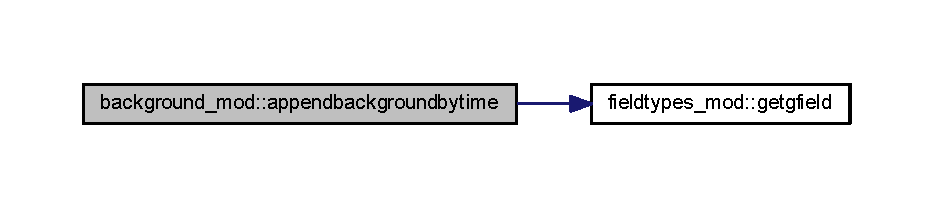
\includegraphics[width=350pt]{namespacebackground__mod_a02fa44cb4575159362bfa3b55520d387_cgraph}
\end{center}
\end{figure}
\mbox{\Hypertarget{namespacebackground__mod_af2f517e4aa946491744e012153045bd4}\label{namespacebackground__mod_af2f517e4aa946491744e012153045bd4}} 
\index{background\+\_\+mod@{background\+\_\+mod}!check@{check}}
\index{check@{check}!background\+\_\+mod@{background\+\_\+mod}}
\subsubsection{\texorpdfstring{check()}{check()}}
{\footnotesize\ttfamily logical function background\+\_\+mod\+::check (\begin{DoxyParamCaption}\item[{class(\mbox{\hyperlink{structbackground__mod_1_1background__class}{background\+\_\+class}}), intent(in)}]{self }\end{DoxyParamCaption})\hspace{0.3cm}{\ttfamily [private]}}



Method that checks the internal consistency of the fields within the background. 

\begin{DoxyAuthor}{Author}
Ricardo Birjukovs Canelas -\/ M\+A\+R\+E\+T\+EC 
\end{DoxyAuthor}


Definition at line 784 of file background.\+f90.


\begin{DoxyCode}
784     \textcolor{keywordtype}{class}(background\_class), \textcolor{keywordtype}{intent(in)} :: self
785     \textcolor{keywordtype}{integer}, \textcolor{keywordtype}{allocatable}, \textcolor{keywordtype}{dimension(:)} :: dimSize, fieldShape
786     \textcolor{keywordtype}{class}(*), \textcolor{keywordtype}{pointer} :: aField
787     \textcolor{keywordtype}{logical} :: equal
788     \textcolor{keywordtype}{integer} :: i
789     \textcolor{keywordtype}{type}(string) :: outext
790     check = .true.
791     equal = .true.
792     \textcolor{keywordflow}{if} (.not.self%initialized) check = .false.
793     \textcolor{keyword}{allocate}(dimsize(\textcolor{keyword}{size}(self%dim)))
794     \textcolor{keyword}{allocate}(fieldshape(\textcolor{keyword}{size}(self%dim)))
795     \textcolor{keywordflow}{do} i=1, \textcolor{keyword}{size}(self%dim)
796         dimsize(i) = \textcolor{keyword}{size}(self%dim(i)%field)
797 \textcolor{keywordflow}{    end do}
798     \textcolor{keyword}{call }self%fields%reset()               \textcolor{comment}{! reset list iterator}
799     \textcolor{keywordflow}{do} \textcolor{keywordflow}{while}(self%fields%moreValues())     \textcolor{comment}{! loop while there are values to process}
800         afield => self%fields%currentValue()
801         \textcolor{keywordflow}{select type}(afield)
802 \textcolor{keywordflow}{        class is} (field\_class)
803             equal = all(dimsize.eq.afield%getFieldShape())
804             \textcolor{keywordflow}{if} (.not.equal) check = .false.
805 \textcolor{keywordflow}{            class default}
806             outext = \textcolor{stringliteral}{'[background\_class::check] Unexepected type of content, not a scalar Field'}
807             \textcolor{keyword}{call }log%put(outext)
808             stop
809 \textcolor{keywordflow}{        end select}
810         \textcolor{keyword}{call }self%fields%next()            \textcolor{comment}{! increment the list iterator}
811 \textcolor{keywordflow}{    end do}
812     \textcolor{keyword}{call }self%fields%reset()               \textcolor{comment}{! reset list iterator}
813 
\end{DoxyCode}
\mbox{\Hypertarget{namespacebackground__mod_a1610fcc9ce260beb3c35418e92a63391}\label{namespacebackground__mod_a1610fcc9ce260beb3c35418e92a63391}} 
\index{background\+\_\+mod@{background\+\_\+mod}!cleanbackground@{cleanbackground}}
\index{cleanbackground@{cleanbackground}!background\+\_\+mod@{background\+\_\+mod}}
\subsubsection{\texorpdfstring{cleanbackground()}{cleanbackground()}}
{\footnotesize\ttfamily subroutine background\+\_\+mod\+::cleanbackground (\begin{DoxyParamCaption}\item[{class(\mbox{\hyperlink{structbackground__mod_1_1background__class}{background\+\_\+class}}), intent(inout)}]{self }\end{DoxyParamCaption})\hspace{0.3cm}{\ttfamily [private]}}



Method that cleans all data in the Background object. 

\begin{DoxyAuthor}{Author}
Ricardo Birjukovs Canelas -\/ M\+A\+R\+E\+T\+EC 
\end{DoxyAuthor}


Definition at line 569 of file background.\+f90.


\begin{DoxyCode}
569     \textcolor{keywordtype}{class}(background\_class), \textcolor{keywordtype}{intent(inout)} :: self
570     self%initialized = .false.
571     self%id = mv\_int
572     self%name = \textcolor{stringliteral}{''}
573     \textcolor{keywordflow}{if} (\textcolor{keyword}{allocated}(self%dim)) \textcolor{keyword}{deallocate}(self%dim)
574     \textcolor{keyword}{call }self%cleanFields()
575     \textcolor{keyword}{call }self%fields%finalize()
\end{DoxyCode}
\mbox{\Hypertarget{namespacebackground__mod_a843a471a68ce83809e3ed0a40886a4e7}\label{namespacebackground__mod_a843a471a68ce83809e3ed0a40886a4e7}} 
\index{background\+\_\+mod@{background\+\_\+mod}!cleanfields@{cleanfields}}
\index{cleanfields@{cleanfields}!background\+\_\+mod@{background\+\_\+mod}}
\subsubsection{\texorpdfstring{cleanfields()}{cleanfields()}}
{\footnotesize\ttfamily subroutine background\+\_\+mod\+::cleanfields (\begin{DoxyParamCaption}\item[{class(\mbox{\hyperlink{structbackground__mod_1_1background__class}{background\+\_\+class}}), intent(inout)}]{self }\end{DoxyParamCaption})\hspace{0.3cm}{\ttfamily [private]}}



Method that cleans all data in the Background object fields. 

\begin{DoxyAuthor}{Author}
Ricardo Birjukovs Canelas -\/ M\+A\+R\+E\+T\+EC 
\end{DoxyAuthor}


Definition at line 584 of file background.\+f90.


\begin{DoxyCode}
584     \textcolor{keywordtype}{class}(background\_class), \textcolor{keywordtype}{intent(inout)} :: self
585     \textcolor{keywordtype}{class}(*), \textcolor{keywordtype}{pointer} :: curr
586     \textcolor{keywordtype}{type}(string) :: outext
587     \textcolor{keyword}{call }self%fields%reset()               \textcolor{comment}{! reset list iterator}
588     \textcolor{keywordflow}{do} \textcolor{keywordflow}{while}(self%fields%moreValues())     \textcolor{comment}{! loop while there are values}
589         curr => self%fields%currentValue() \textcolor{comment}{! get current value}
590         \textcolor{keywordflow}{select type}(curr)
591 \textcolor{keywordflow}{        class is} (scalar1d\_field\_class)
592             \textcolor{keyword}{call }curr%finalize()
593 \textcolor{keywordflow}{        class is} (scalar2d\_field\_class)
594             \textcolor{keyword}{call }curr%finalize()
595 \textcolor{keywordflow}{        class is} (scalar3d\_field\_class)
596             \textcolor{keyword}{call }curr%finalize()
597 \textcolor{keywordflow}{        class is} (scalar4d\_field\_class)
598             \textcolor{keyword}{call }curr%finalize()
599 \textcolor{keywordflow}{            class default}
600             outext = \textcolor{stringliteral}{'[background\_class::cleanFields] Unexepected type of content, not a scalar Field'}
601             \textcolor{keyword}{call }log%put(outext)
602             stop
603 \textcolor{keywordflow}{        end select}
604         \textcolor{keyword}{call }self%fields%next()            \textcolor{comment}{! increment the list iterator}
605         \textcolor{keyword}{nullify}(curr)
606 \textcolor{keywordflow}{    end do}
607     \textcolor{keyword}{call }self%fields%reset()               \textcolor{comment}{! reset list iterator}
\end{DoxyCode}
\mbox{\Hypertarget{namespacebackground__mod_ad0096fb6a5a11854fd70a7ce58dc3000}\label{namespacebackground__mod_ad0096fb6a5a11854fd70a7ce58dc3000}} 
\index{background\+\_\+mod@{background\+\_\+mod}!constructor@{constructor}}
\index{constructor@{constructor}!background\+\_\+mod@{background\+\_\+mod}}
\subsubsection{\texorpdfstring{constructor()}{constructor()}}
{\footnotesize\ttfamily type(\mbox{\hyperlink{structbackground__mod_1_1background__class}{background\+\_\+class}}) function background\+\_\+mod\+::constructor (\begin{DoxyParamCaption}\item[{integer, intent(in)}]{id,  }\item[{type(string), intent(in)}]{name,  }\item[{type(\mbox{\hyperlink{structgeometry__mod_1_1box}{box}}), intent(in)}]{extents,  }\item[{type(scalar1d\+\_\+field\+\_\+class), dimension(\+:), intent(in)}]{dims }\end{DoxyParamCaption})\hspace{0.3cm}{\ttfamily [private]}}



Constructor for Background object. 

\begin{DoxyAuthor}{Author}
Ricardo Birjukovs Canelas -\/ M\+A\+R\+E\+T\+EC 
\end{DoxyAuthor}

\begin{DoxyParams}[1]{Parameters}
\mbox{\tt in}  & {\em id,name,extents,dims} & \\
\hline
\end{DoxyParams}


Definition at line 99 of file background.\+f90.


\begin{DoxyCode}
99     \textcolor{keywordtype}{type}(background\_class) :: constructor
100     \textcolor{keywordtype}{integer}, \textcolor{keywordtype}{intent(in)} :: id
101     \textcolor{keywordtype}{type}(string), \textcolor{keywordtype}{intent(in)} :: name
102     \textcolor{keywordtype}{type}(box), \textcolor{keywordtype}{intent(in)} :: extents
103     \textcolor{keywordtype}{type}(scalar1d\_field\_class), \textcolor{keywordtype}{dimension(:)}, \textcolor{keywordtype}{intent(in)} :: dims
104     constructor%initialized = .true.
105     \textcolor{keyword}{call }constructor%setID(id, name)
106     \textcolor{keyword}{call }constructor%setExtents(extents)
107     \textcolor{keyword}{call }constructor%setDims(dims)
\end{DoxyCode}
Here is the caller graph for this function\+:
\nopagebreak
\begin{figure}[H]
\begin{center}
\leavevmode
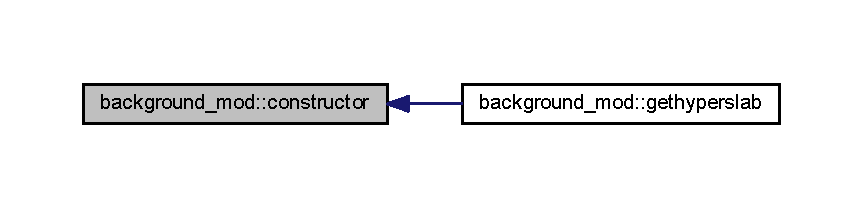
\includegraphics[width=350pt]{namespacebackground__mod_ad0096fb6a5a11854fd70a7ce58dc3000_icgraph}
\end{center}
\end{figure}
\mbox{\Hypertarget{namespacebackground__mod_a64c3966a113bc0f3b603c591bc345ca1}\label{namespacebackground__mod_a64c3966a113bc0f3b603c591bc345ca1}} 
\index{background\+\_\+mod@{background\+\_\+mod}!getdimextents@{getdimextents}}
\index{getdimextents@{getdimextents}!background\+\_\+mod@{background\+\_\+mod}}
\subsubsection{\texorpdfstring{getdimextents()}{getdimextents()}}
{\footnotesize\ttfamily real(prec) function, dimension(2) background\+\_\+mod\+::getdimextents (\begin{DoxyParamCaption}\item[{class(\mbox{\hyperlink{structbackground__mod_1_1background__class}{background\+\_\+class}}), intent(in)}]{self,  }\item[{type(string), intent(in)}]{name,  }\item[{logical, intent(in), optional}]{mandatory }\end{DoxyParamCaption})\hspace{0.3cm}{\ttfamily [private]}}



Method that returns two reals, min and max of a given dimension. 

\begin{DoxyAuthor}{Author}
Ricardo Birjukovs Canelas -\/ M\+A\+R\+E\+T\+EC 
\end{DoxyAuthor}

\begin{DoxyParams}[1]{Parameters}
\mbox{\tt in}  & {\em self,name,mandatory} & \\
\hline
\end{DoxyParams}


Definition at line 151 of file background.\+f90.


\begin{DoxyCode}
151     \textcolor{keywordtype}{class}(background\_class), \textcolor{keywordtype}{intent(in)} :: self
152     \textcolor{keywordtype}{type}(string), \textcolor{keywordtype}{intent(in)} :: name
153     \textcolor{keywordtype}{logical}, \textcolor{keywordtype}{optional}, \textcolor{keywordtype}{intent(in)} :: mandatory
154     \textcolor{keywordtype}{logical} :: mand
155     \textcolor{keywordtype}{integer} :: i
156     \textcolor{keywordtype}{real(prec)} :: dimExtent(2)
157     mand = .true.
158     \textcolor{keywordflow}{if} (\textcolor{keyword}{present}(mandatory)) mand = mandatory
159     i = self%getDimIndex(name, mand)
160     \textcolor{keywordflow}{if} ( i/= mv\_int) \textcolor{keywordflow}{then}
161         dimextent(1) = self%dim(i)%getFieldMinBound()
162         dimextent(2) = self%dim(i)%getFieldMaxBound()
163     \textcolor{keywordflow}{else}
164         dimextent(1) = mv
165         dimextent(2) = mv
166 \textcolor{keywordflow}{    end if}
\end{DoxyCode}
\mbox{\Hypertarget{namespacebackground__mod_a8a4c5fdcda63376bc3a984e9612dfb63}\label{namespacebackground__mod_a8a4c5fdcda63376bc3a984e9612dfb63}} 
\index{background\+\_\+mod@{background\+\_\+mod}!getdimindex@{getdimindex}}
\index{getdimindex@{getdimindex}!background\+\_\+mod@{background\+\_\+mod}}
\subsubsection{\texorpdfstring{getdimindex()}{getdimindex()}}
{\footnotesize\ttfamily integer function background\+\_\+mod\+::getdimindex (\begin{DoxyParamCaption}\item[{class(\mbox{\hyperlink{structbackground__mod_1_1background__class}{background\+\_\+class}}), intent(in)}]{self,  }\item[{type(string), intent(in)}]{name,  }\item[{logical, intent(in), optional}]{mandatory }\end{DoxyParamCaption})\hspace{0.3cm}{\ttfamily [private]}}



Method that returns the index of a given dimension by it\textquotesingle{}s name. 

\begin{DoxyAuthor}{Author}
Ricardo Birjukovs Canelas -\/ M\+A\+R\+E\+T\+EC 
\end{DoxyAuthor}

\begin{DoxyParams}[1]{Parameters}
\mbox{\tt in}  & {\em self,name,mandatory} & \\
\hline
\end{DoxyParams}


Definition at line 117 of file background.\+f90.


\begin{DoxyCode}
117     \textcolor{keywordtype}{class}(background\_class), \textcolor{keywordtype}{intent(in)} :: self
118     \textcolor{keywordtype}{type}(string), \textcolor{keywordtype}{intent(in)} :: name
119     \textcolor{keywordtype}{logical}, \textcolor{keywordtype}{optional}, \textcolor{keywordtype}{intent(in)} :: mandatory
120     \textcolor{keywordtype}{integer} :: i
121     \textcolor{keywordtype}{type}(string) :: outext
122     \textcolor{keywordtype}{logical} found
123     found = .false.
124     \textcolor{keywordflow}{do} i=1, \textcolor{keyword}{size}(self%dim)
125         \textcolor{keywordflow}{if} (self%dim(i)%name == name) \textcolor{keywordflow}{then}
126             found = .true.
127             getdimindex = i
128             \textcolor{keywordflow}{return}
129 \textcolor{keywordflow}{        end if}
130 \textcolor{keywordflow}{    end do}
131     \textcolor{keywordflow}{if} (\textcolor{keyword}{present}(mandatory)) \textcolor{keywordflow}{then}
132         \textcolor{keywordflow}{if} (mandatory) \textcolor{keywordflow}{then}
133             \textcolor{keywordflow}{if} (.not. found) \textcolor{keywordflow}{then}
134                 outext = \textcolor{stringliteral}{'[background\_class::getDimIndex]: Field dimensions dont contain a field called '}//
       name //\textcolor{stringliteral}{', stoping'}
135                 \textcolor{keyword}{call }log%put(outext)
136                 stop
137 \textcolor{keywordflow}{            end if}
138         \textcolor{keywordflow}{else}
139             getdimindex = mv\_int
140 \textcolor{keywordflow}{        end if}
141 \textcolor{keywordflow}{    end if}
\end{DoxyCode}
\mbox{\Hypertarget{namespacebackground__mod_ae26fda3baab915148ec5749d1eda2ea6}\label{namespacebackground__mod_ae26fda3baab915148ec5749d1eda2ea6}} 
\index{background\+\_\+mod@{background\+\_\+mod}!gethyperslab@{gethyperslab}}
\index{gethyperslab@{gethyperslab}!background\+\_\+mod@{background\+\_\+mod}}
\subsubsection{\texorpdfstring{gethyperslab()}{gethyperslab()}}
{\footnotesize\ttfamily type(\mbox{\hyperlink{structbackground__mod_1_1background__class}{background\+\_\+class}}) function background\+\_\+mod\+::gethyperslab (\begin{DoxyParamCaption}\item[{class(\mbox{\hyperlink{structbackground__mod_1_1background__class}{background\+\_\+class}}), intent(in)}]{self,  }\item[{type(\mbox{\hyperlink{structgeometry__mod_1_1box}{box}}), intent(in)}]{domain,  }\item[{real(prec), dimension(2), intent(in), optional}]{time }\end{DoxyParamCaption})\hspace{0.3cm}{\ttfamily [private]}}



returns a background as a subset of another 

\begin{DoxyAuthor}{Author}
Ricardo Birjukovs Canelas -\/ M\+A\+R\+E\+T\+EC 
\end{DoxyAuthor}

\begin{DoxyParams}[1]{Parameters}
\mbox{\tt in}  & {\em self,domain,time} & \\
\hline
\end{DoxyParams}


Definition at line 276 of file background.\+f90.


\begin{DoxyCode}
276     \textcolor{keywordtype}{class}(background\_class), \textcolor{keywordtype}{intent(in)} :: self
277     \textcolor{keywordtype}{type}(box), \textcolor{keywordtype}{intent(in)} :: domain
278     \textcolor{keywordtype}{real(prec)}, \textcolor{keywordtype}{intent(in)}, \textcolor{keywordtype}{optional} :: time(2)
279     \textcolor{keywordtype}{real(prec)} :: ltime(2)
280     \textcolor{keywordtype}{type}(scalar1d\_field\_class), \textcolor{keywordtype}{allocatable}, \textcolor{keywordtype}{dimension(:)} :: backgrounDims
281     \textcolor{keywordtype}{type}(generic\_field\_class), \textcolor{keywordtype}{allocatable}, \textcolor{keywordtype}{dimension(:)} :: gfield
282     \textcolor{keywordtype}{class}(*), \textcolor{keywordtype}{pointer} :: curr
283     \textcolor{keywordtype}{type}(box) :: extents
284     \textcolor{keywordtype}{type}(vector) :: pt
285     \textcolor{keywordtype}{real(prec)}, \textcolor{keywordtype}{dimension(3,2)} :: dimExtents
286     \textcolor{keywordtype}{integer}, \textcolor{keywordtype}{allocatable}, \textcolor{keywordtype}{dimension(:)} :: llbound
287     \textcolor{keywordtype}{integer}, \textcolor{keywordtype}{allocatable}, \textcolor{keywordtype}{dimension(:)} :: uubound
288     \textcolor{keywordtype}{integer} :: temp\_int
289     \textcolor{keywordtype}{type}(string) :: outext
290     \textcolor{keywordtype}{integer} :: i
291 
292     ltime = self%getDimExtents(globals%Var%time)
293     \textcolor{keywordflow}{if} (\textcolor{keyword}{present}(time)) ltime = time
294     \textcolor{comment}{!finding index bounds of the slicing geometry}
295     \textcolor{keyword}{allocate}(llbound(\textcolor{keyword}{size}(self%dim)))
296     \textcolor{keyword}{allocate}(uubound(\textcolor{keyword}{size}(self%dim)))
297     llbound = self%getPointDimIndexes(domain%pt, ltime(1))
298     uubound = self%getPointDimIndexes(domain%pt+domain%size, ltime(2))
299     \textcolor{comment}{!slicing dimensions}
300     \textcolor{keyword}{allocate}(backgroundims(\textcolor{keyword}{size}(self%dim)))
301     \textcolor{keywordflow}{do} i=1, \textcolor{keyword}{size}(self%dim)
302         \textcolor{keywordflow}{if} (llbound(i) > uubound(i)) \textcolor{keywordflow}{then} \textcolor{comment}{!because We're not inverting the dimension and fields - Needs to
       be corrected}
303             temp\_int = llbound(i)
304             llbound(i) = uubound(i)
305             uubound(i) = temp\_int
306 \textcolor{keywordflow}{        end if}
307         llbound(i) = max(1, llbound(i)-1) \textcolor{comment}{!adding safety net to index bounds}
308         uubound(i) = min(uubound(i)+1, \textcolor{keyword}{size}(self%dim(i)%field))
309         \textcolor{keyword}{call }backgroundims(i)%initialize(self%dim(i)%name, self%dim(i)%units, 1, self%getSlabDim(i, llbound
      (i), uubound(i)))
310 \textcolor{keywordflow}{    end do}
311     \textcolor{comment}{!slicing variables}
312     \textcolor{keyword}{allocate}(gfield(self%fields%getSize()))
313     i=1
314     \textcolor{keyword}{call }self%fields%reset()               \textcolor{comment}{! reset list iterator}
315     \textcolor{keywordflow}{do} \textcolor{keywordflow}{while}(self%fields%moreValues())     \textcolor{comment}{! loop while there are values}
316         curr => self%fields%currentValue() \textcolor{comment}{! get current value}
317         \textcolor{keywordflow}{select type}(curr)
318 \textcolor{keywordflow}{        class is} (field\_class)
319             gfield(i) = curr%getFieldSlice(llbound, uubound)
320 \textcolor{keywordflow}{            class default}
321             outext = \textcolor{stringliteral}{'[background\_class::getHyperSlab] Unexepected type of content, not a scalar Field'}
322             \textcolor{keyword}{call }log%put(outext)
323             stop
324 \textcolor{keywordflow}{        end select}
325         \textcolor{keyword}{call }self%fields%next()            \textcolor{comment}{! increment the list iterator}
326         i = i+1
327         \textcolor{keyword}{nullify}(curr)
328 \textcolor{keywordflow}{    end do}
329     \textcolor{keyword}{call }self%fields%reset()               \textcolor{comment}{! reset list iterator}
330     \textcolor{comment}{!creating bounding box}
331     dimextents = 0.0
332     \textcolor{keywordflow}{do} i = 1, \textcolor{keyword}{size}(backgroundims)
333         \textcolor{keywordflow}{if} (backgroundims(i)%name == globals%Var%lon) \textcolor{keywordflow}{then}
334             dimextents(1,1) = backgroundims(i)%getFieldMinBound()
335             dimextents(1,2) = backgroundims(i)%getFieldMaxBound()
336         \textcolor{keywordflow}{else} \textcolor{keywordflow}{if} (backgroundims(i)%name == globals%Var%lat) \textcolor{keywordflow}{then}
337             dimextents(2,1) = backgroundims(i)%getFieldMinBound()
338             dimextents(2,2) = backgroundims(i)%getFieldMaxBound()
339         \textcolor{keywordflow}{else} \textcolor{keywordflow}{if} (backgroundims(i)%name == globals%Var%level) \textcolor{keywordflow}{then}
340             dimextents(3,1) = backgroundims(i)%getFieldMinBound()
341             dimextents(3,2) = backgroundims(i)%getFieldMaxBound()
342 \textcolor{keywordflow}{        end if}
343 \textcolor{keywordflow}{    end do}
344     extents%pt = dimextents(1,1)*ex + dimextents(2,1)*ey + dimextents(3,1)*ez
345     pt = dimextents(1,2)*ex + dimextents(2,2)*ey + dimextents(3,2)*ez
346     extents%size = pt - extents%pt
347     \textcolor{comment}{!creating the sliced background}
348     gethyperslab = constructor(1, self%name, extents, backgroundims)
349     \textcolor{keywordflow}{do} i=1, \textcolor{keyword}{size}(gfield)
350         \textcolor{keyword}{call }gethyperslab%add(gfield(i))
351         \textcolor{keyword}{call }gfield(i)%finalize()
352 \textcolor{keywordflow}{    end do}
353 
354     \textcolor{keywordflow}{if}(.not.self%check()) \textcolor{keywordflow}{then}
355         outext = \textcolor{stringliteral}{'[Background::getHyperSlab]: non-conformant Background, stoping '}
356         \textcolor{keyword}{call }log%put(outext)
357         stop
358 \textcolor{keywordflow}{    end if}
359 
\end{DoxyCode}
Here is the call graph for this function\+:
\nopagebreak
\begin{figure}[H]
\begin{center}
\leavevmode
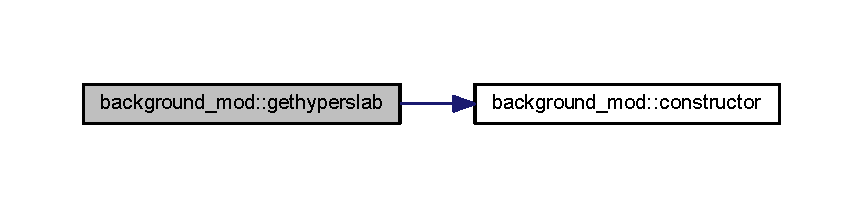
\includegraphics[width=350pt]{namespacebackground__mod_ae26fda3baab915148ec5749d1eda2ea6_cgraph}
\end{center}
\end{figure}
\mbox{\Hypertarget{namespacebackground__mod_ac799224ce7ad219bf1fb4f1f42508f45}\label{namespacebackground__mod_ac799224ce7ad219bf1fb4f1f42508f45}} 
\index{background\+\_\+mod@{background\+\_\+mod}!getpointdimindexes@{getpointdimindexes}}
\index{getpointdimindexes@{getpointdimindexes}!background\+\_\+mod@{background\+\_\+mod}}
\subsubsection{\texorpdfstring{getpointdimindexes()}{getpointdimindexes()}}
{\footnotesize\ttfamily integer function, dimension(\+:), allocatable background\+\_\+mod\+::getpointdimindexes (\begin{DoxyParamCaption}\item[{class(\mbox{\hyperlink{structbackground__mod_1_1background__class}{background\+\_\+class}}), intent(in)}]{self,  }\item[{type(vector), intent(in)}]{pt,  }\item[{real(prec), intent(in)}]{time }\end{DoxyParamCaption})\hspace{0.3cm}{\ttfamily [private]}}



returns the indexes of the dims for a given point 

\begin{DoxyAuthor}{Author}
Ricardo Birjukovs Canelas -\/ M\+A\+R\+E\+T\+EC 
\end{DoxyAuthor}

\begin{DoxyParams}[1]{Parameters}
\mbox{\tt in}  & {\em self,pt,time} & \\
\hline
\end{DoxyParams}


Definition at line 369 of file background.\+f90.


\begin{DoxyCode}
369     \textcolor{keywordtype}{class}(background\_class), \textcolor{keywordtype}{intent(in)} :: self
370     \textcolor{keywordtype}{type}(vector), \textcolor{keywordtype}{intent(in)} :: pt
371     \textcolor{keywordtype}{real(prec)}, \textcolor{keywordtype}{intent(in)} :: time
372     \textcolor{keywordtype}{integer}, \textcolor{keywordtype}{allocatable}, \textcolor{keywordtype}{dimension(:)} :: getPointDimIndexes
373     \textcolor{keywordtype}{integer} :: i
374     \textcolor{keyword}{allocate}(getpointdimindexes(\textcolor{keyword}{size}(self%dim)))
375     \textcolor{keywordflow}{do} i= 1, \textcolor{keyword}{size}(self%dim)
376         \textcolor{keywordflow}{if} (self%dim(i)%name == globals%Var%lon) getpointdimindexes(i) = self%dim(i)%getFieldNearestIndex(
      pt%x)
377         \textcolor{keywordflow}{if} (self%dim(i)%name == globals%Var%lat) getpointdimindexes(i) = self%dim(i)%getFieldNearestIndex(
      pt%y)
378         \textcolor{keywordflow}{if} (self%dim(i)%name == globals%Var%level) getpointdimindexes(i) = self%dim(i)%getFieldNearestIndex
      (pt%z)
379         \textcolor{keywordflow}{if} (self%dim(i)%name == globals%Var%time)  getpointdimindexes(i) = self%dim(i)%getFieldNearestIndex
      (time)
380 \textcolor{keywordflow}{    end do}
\end{DoxyCode}
\mbox{\Hypertarget{namespacebackground__mod_a09d61976c4545e8753eb4594044b109d}\label{namespacebackground__mod_a09d61976c4545e8753eb4594044b109d}} 
\index{background\+\_\+mod@{background\+\_\+mod}!getslabdim@{getslabdim}}
\index{getslabdim@{getslabdim}!background\+\_\+mod@{background\+\_\+mod}}
\subsubsection{\texorpdfstring{getslabdim()}{getslabdim()}}
{\footnotesize\ttfamily real(prec) function, dimension(\+:), allocatable background\+\_\+mod\+::getslabdim (\begin{DoxyParamCaption}\item[{class(\mbox{\hyperlink{structbackground__mod_1_1background__class}{background\+\_\+class}}), intent(in)}]{self,  }\item[{integer, intent(in)}]{num\+Dim,  }\item[{integer, intent(in)}]{llbound,  }\item[{integer, intent(in)}]{uubound }\end{DoxyParamCaption})\hspace{0.3cm}{\ttfamily [private]}}



returns an array witn a sliced dimension 

\begin{DoxyAuthor}{Author}
Ricardo Birjukovs Canelas -\/ M\+A\+R\+E\+T\+EC 
\end{DoxyAuthor}

\begin{DoxyParams}[1]{Parameters}
\mbox{\tt in}  & {\em self,domain,time} & \\
\hline
\end{DoxyParams}


Definition at line 390 of file background.\+f90.


\begin{DoxyCode}
390     \textcolor{keywordtype}{class}(background\_class), \textcolor{keywordtype}{intent(in)} :: self
391     \textcolor{keywordtype}{integer}, \textcolor{keywordtype}{intent(in)} :: numDim, llbound, uubound
392     \textcolor{keywordtype}{real(prec)}, \textcolor{keywordtype}{allocatable}, \textcolor{keywordtype}{dimension(:)} :: getSlabDim
393     \textcolor{keyword}{allocate}(getslabdim, source = self%dim(numdim)%field(llbound:uubound))
\end{DoxyCode}
\mbox{\Hypertarget{namespacebackground__mod_ad6c54d2cf1d1981fb928cd14d387aa8b}\label{namespacebackground__mod_ad6c54d2cf1d1981fb928cd14d387aa8b}} 
\index{background\+\_\+mod@{background\+\_\+mod}!makelandmask@{makelandmask}}
\index{makelandmask@{makelandmask}!background\+\_\+mod@{background\+\_\+mod}}
\subsubsection{\texorpdfstring{makelandmask()}{makelandmask()}}
{\footnotesize\ttfamily subroutine background\+\_\+mod\+::makelandmask (\begin{DoxyParamCaption}\item[{class(\mbox{\hyperlink{structbackground__mod_1_1background__class}{background\+\_\+class}}), intent(inout)}]{self }\end{DoxyParamCaption})\hspace{0.3cm}{\ttfamily [private]}}



Method to use a stored binary field to make a land mask used for land interaction\+: bed settling, beaching, ... 

\begin{DoxyAuthor}{Author}
Ricardo Birjukovs Canelas -\/ M\+A\+R\+E\+T\+EC 
\end{DoxyAuthor}


Definition at line 488 of file background.\+f90.


\begin{DoxyCode}
488     \textcolor{keywordtype}{class}(background\_class), \textcolor{keywordtype}{intent(inout)} :: self
489     \textcolor{keywordtype}{class}(*), \textcolor{keywordtype}{pointer} :: curr
490     \textcolor{keywordtype}{logical}, \textcolor{keywordtype}{allocatable}, \textcolor{keywordtype}{dimension(:,:,:)} :: shiftleftlon3d, shiftuplat3d, shiftrigthlon3d, shiftdownlat3d
      , beach3d
491     \textcolor{keywordtype}{logical}, \textcolor{keywordtype}{allocatable}, \textcolor{keywordtype}{dimension(:,:,:,:)} :: shiftleftlon4d, shiftuplat4d, shiftrigthlon4d, 
      shiftdownlat4d, shiftUpLevel, shiftDownLevel, beach4d, bed4d
492     \textcolor{keywordtype}{type}(string) :: outext
493     \textcolor{keywordtype}{integer} :: dimIndx
494     \textcolor{keyword}{call }self%fields%reset()               \textcolor{comment}{! reset list iterator}
495     \textcolor{keywordflow}{do} \textcolor{keywordflow}{while}(self%fields%moreValues())     \textcolor{comment}{! loop while there are values}
496         curr => self%fields%currentValue() \textcolor{comment}{! get current value        }
497             \textcolor{keywordflow}{select type}(curr)            
498 \textcolor{keywordflow}{            class is} (scalar3d\_field\_class)
499                 \textcolor{keywordflow}{if} (curr%name == globals%Var%landIntMask) \textcolor{keywordflow}{then}
500                     \textcolor{keyword}{allocate}(shiftleftlon3d(\textcolor{keyword}{size}(curr%field,1), \textcolor{keyword}{size}(curr%field,2), \textcolor{keyword}{size}(curr%field,3)))
501                     \textcolor{keyword}{allocate}(shiftuplat3d(\textcolor{keyword}{size}(curr%field,1), \textcolor{keyword}{size}(curr%field,2), \textcolor{keyword}{size}(curr%field,3)))
502                     \textcolor{keyword}{allocate}(shiftrigthlon3d(\textcolor{keyword}{size}(curr%field,1), \textcolor{keyword}{size}(curr%field,2), \textcolor{keyword}{size}(curr%field,3)))
503                     \textcolor{keyword}{allocate}(shiftdownlat3d(\textcolor{keyword}{size}(curr%field,1), \textcolor{keyword}{size}(curr%field,2), \textcolor{keyword}{size}(curr%field,3)))
504                     \textcolor{keyword}{allocate}(beach3d(\textcolor{keyword}{size}(curr%field,1), \textcolor{keyword}{size}(curr%field,2), \textcolor{keyword}{size}(curr%field,3)))
505                     shiftleftlon3d = .false.
506                     shiftleftlon3d(:\textcolor{keyword}{size}(curr%field,1)-1,:,:) = abs(curr%field(:\textcolor{keyword}{size}(curr%field,1)-1,:,:) -
       curr%field(2:,:,:)) == globals%Mask%waterVal - globals%Mask%landVal
507                     shiftrigthlon3d = .false.
508                     shiftrigthlon3d(2:,:,:) = abs(curr%field(2:,:,:) - curr%field(:\textcolor{keyword}{size}(curr%field,1)-1,:,:
      )) == globals%Mask%waterVal - globals%Mask%landVal
509                     shiftuplat3d = .false.
510                     shiftuplat3d(:,:\textcolor{keyword}{size}(curr%field,2)-1,:) = abs(curr%field(:,:\textcolor{keyword}{size}(curr%field,2)-1,:) - 
      curr%field(:,2:,:)) == globals%Mask%waterVal - globals%Mask%landVal
511                     shiftdownlat3d = .false.
512                     shiftdownlat3d(:, 2:,:) = abs(curr%field(:,2:,:) - curr%field(:,:\textcolor{keyword}{size}(curr%field,2)-1,:
      )) == globals%Mask%waterVal - globals%Mask%landVal
513                     beach3d = .false.
514                     beach3d = shiftleftlon3d .or. shiftrigthlon3d .or. shiftuplat3d .or. shiftdownlat3d \textcolor{comment}{
      !colapsing all the shifts}
515                     beach3d = beach3d .and. (curr%field == globals%Mask%landVal) \textcolor{comment}{!just points that were
       already wet}
516                     \textcolor{keywordflow}{where}(beach3d) curr%field = globals%Mask%beachVal
517 \textcolor{keywordflow}{                end if}
518 \textcolor{keywordflow}{            class is} (scalar4d\_field\_class)
519                 \textcolor{keywordflow}{if} (curr%name == globals%Var%landIntMask) \textcolor{keywordflow}{then}
520                     \textcolor{keyword}{allocate}(shiftleftlon4d(\textcolor{keyword}{size}(curr%field,1), \textcolor{keyword}{size}(curr%field,2), \textcolor{keyword}{size}(curr%field,3), \textcolor{keyword}{
      size}(curr%field,4)))
521                     \textcolor{keyword}{allocate}(shiftuplat4d(\textcolor{keyword}{size}(curr%field,1), \textcolor{keyword}{size}(curr%field,2), \textcolor{keyword}{size}(curr%field,3), \textcolor{keyword}{size}(
      curr%field,4)))
522                     \textcolor{keyword}{allocate}(shiftrigthlon4d(\textcolor{keyword}{size}(curr%field,1), \textcolor{keyword}{size}(curr%field,2), \textcolor{keyword}{size}(curr%field,3), \textcolor{keyword}{
      size}(curr%field,4)))
523                     \textcolor{keyword}{allocate}(shiftdownlat4d(\textcolor{keyword}{size}(curr%field,1), \textcolor{keyword}{size}(curr%field,2), \textcolor{keyword}{size}(curr%field,3), \textcolor{keyword}{
      size}(curr%field,4)))
524                     \textcolor{keyword}{allocate}(shiftuplevel(\textcolor{keyword}{size}(curr%field,1), \textcolor{keyword}{size}(curr%field,2), \textcolor{keyword}{size}(curr%field,3), \textcolor{keyword}{size}(
      curr%field,4)))
525                     \textcolor{keyword}{allocate}(shiftdownlevel(\textcolor{keyword}{size}(curr%field,1), \textcolor{keyword}{size}(curr%field,2), \textcolor{keyword}{size}(curr%field,3), \textcolor{keyword}{
      size}(curr%field,4)))
526                     \textcolor{keyword}{allocate}(beach4d(\textcolor{keyword}{size}(curr%field,1), \textcolor{keyword}{size}(curr%field,2), \textcolor{keyword}{size}(curr%field,3), \textcolor{keyword}{size}(curr
      %field,4)))
527                     \textcolor{keyword}{allocate}(bed4d(\textcolor{keyword}{size}(curr%field,1), \textcolor{keyword}{size}(curr%field,2), \textcolor{keyword}{size}(curr%field,3), \textcolor{keyword}{size}(curr
      %field,4)))
528                     shiftleftlon4d = .false.
529                     shiftleftlon4d(:\textcolor{keyword}{size}(curr%field,1)-1,:,:,:) = abs(curr%field(:\textcolor{keyword}{size}(curr%field,1)-1,:,:,
      :) - curr%field(2:,:,:,:)) /= 0.0
530                     shiftrigthlon4d = .false.
531                     shiftrigthlon4d(2:,:,:,:) = abs(curr%field(2:,:,:,:) - curr%field(:\textcolor{keyword}{size}(curr%field,1)-1
      ,:,:,:)) /= 0.0
532                     shiftdownlat4d = .false.
533                     shiftdownlat4d(:,:\textcolor{keyword}{size}(curr%field,2)-1,:,:) = abs(curr%field(:,:\textcolor{keyword}{size}(curr%field,2)-1,:,
      :) - curr%field(:,2:,:,:)) /= 0.0
534                     shiftuplat4d = .false.
535                     shiftuplat4d(:,2:,:,:) = abs(curr%field(:,2:,:,:) - curr%field(:,:\textcolor{keyword}{size}(curr%field,2)-1,
      :,:)) /= 0.0
536                     shiftuplevel = .false.
537                     shiftuplevel(:,:,2:,:) = abs(curr%field(:,:,2:,:) - curr%field(:,:,:\textcolor{keyword}{size}(curr%field,3)-
      1,:)) /= 0.0
538                     shiftdownlevel = .false.
539                     shiftdownlevel(:,:,:\textcolor{keyword}{size}(curr%field,3)-1,:) = abs(curr%field(:,:,:\textcolor{keyword}{size}(curr%field,3)-1,
      :) - curr%field(:,:,2:,:)) /= 0.0
540                     beach4d = .false.
541                     beach4d = shiftleftlon4d .or. shiftrigthlon4d .or. shiftuplat4d .or. shiftdownlat4d 
      .or. shiftdownlevel .or. shiftuplevel \textcolor{comment}{!colapsing all the shifts                    }
542                     \textcolor{comment}{!beach4d = beach4d .and. (curr%field == Globals%Mask%landVal) !just points that were
       already wet}
543                     bed4d = beach4d
544                     dimindx = self%getDimIndex(globals%Var%level)
545                     dimindx = minloc(abs(self%dim(dimindx)%field - globals%Constants%BeachingLevel),1)
546                     beach4d(:,:,:dimindx,:) = .false. \textcolor{comment}{!this must be above a certain level only}
547                     bed4d(:,:,dimindx:,:) = .false.   \textcolor{comment}{!bellow a certain level}
548                     \textcolor{keywordflow}{where}(beach4d) curr%field = globals%Mask%beachVal
549                     \textcolor{keywordflow}{where}(bed4d) curr%field = globals%Mask%bedVal
550 \textcolor{keywordflow}{                end if}                
551 \textcolor{keywordflow}{                class default}
552                 outext = \textcolor{stringliteral}{'[background\_class::makeLandMask] Unexepected type of content, not a 3D or 4D
       scalar Field'}
553                 \textcolor{keyword}{call }log%put(outext)
554                 stop
555 \textcolor{keywordflow}{            end select}       
556         \textcolor{keyword}{call }self%fields%next()            \textcolor{comment}{! increment the list iterator}
557         \textcolor{keyword}{nullify}(curr)
558 \textcolor{keywordflow}{    end do}
559     \textcolor{keyword}{call }self%fields%reset()               \textcolor{comment}{! reset list iterator}
560     
\end{DoxyCode}
\mbox{\Hypertarget{namespacebackground__mod_acdcc52b4fb298bc145a121f9e8a4b929}\label{namespacebackground__mod_acdcc52b4fb298bc145a121f9e8a4b929}} 
\index{background\+\_\+mod@{background\+\_\+mod}!print\+\_\+fieldlist@{print\+\_\+fieldlist}}
\index{print\+\_\+fieldlist@{print\+\_\+fieldlist}!background\+\_\+mod@{background\+\_\+mod}}
\subsubsection{\texorpdfstring{print\+\_\+fieldlist()}{print\_fieldlist()}}
{\footnotesize\ttfamily subroutine background\+\_\+mod\+::print\+\_\+fieldlist (\begin{DoxyParamCaption}\item[{class(\mbox{\hyperlink{structbackground__mod_1_1fieldslist__class}{fieldslist\+\_\+class}}), intent(in)}]{this }\end{DoxyParamCaption})\hspace{0.3cm}{\ttfamily [private]}}



Method that prints all the links of the list. 

\begin{DoxyAuthor}{Author}
Ricardo Birjukovs Canelas -\/ M\+A\+R\+E\+T\+EC 
\end{DoxyAuthor}


Definition at line 748 of file background.\+f90.


\begin{DoxyCode}
748     \textcolor{keywordtype}{class}(fieldsList\_class), \textcolor{keywordtype}{intent(in)} :: this
749     \textcolor{keyword}{call }this%reset()               \textcolor{comment}{! reset list iterator}
750     \textcolor{keywordflow}{do} \textcolor{keywordflow}{while}(this%moreValues())     \textcolor{comment}{! loop while there are values to print}
751         \textcolor{keyword}{call }this%printCurrent()
752         \textcolor{keyword}{call }this%next()            \textcolor{comment}{! increment the list iterator}
753 \textcolor{keywordflow}{    end do}
754     \textcolor{keyword}{call }this%reset()               \textcolor{comment}{! reset list iterator}
\end{DoxyCode}
\mbox{\Hypertarget{namespacebackground__mod_a2bd18f3830c0667741efd086d36753db}\label{namespacebackground__mod_a2bd18f3830c0667741efd086d36753db}} 
\index{background\+\_\+mod@{background\+\_\+mod}!print\+\_\+fieldlistcurrent@{print\+\_\+fieldlistcurrent}}
\index{print\+\_\+fieldlistcurrent@{print\+\_\+fieldlistcurrent}!background\+\_\+mod@{background\+\_\+mod}}
\subsubsection{\texorpdfstring{print\+\_\+fieldlistcurrent()}{print\_fieldlistcurrent()}}
{\footnotesize\ttfamily subroutine background\+\_\+mod\+::print\+\_\+fieldlistcurrent (\begin{DoxyParamCaption}\item[{class(\mbox{\hyperlink{structbackground__mod_1_1fieldslist__class}{fieldslist\+\_\+class}}), intent(in)}]{this }\end{DoxyParamCaption})\hspace{0.3cm}{\ttfamily [private]}}



Method that prints the current link of the list. 

\begin{DoxyAuthor}{Author}
Ricardo Birjukovs Canelas -\/ M\+A\+R\+E\+T\+EC 
\end{DoxyAuthor}


Definition at line 763 of file background.\+f90.


\begin{DoxyCode}
763     \textcolor{keywordtype}{class}(fieldsList\_class), \textcolor{keywordtype}{intent(in)} :: this
764     \textcolor{keywordtype}{class}(*), \textcolor{keywordtype}{pointer} :: curr
765     \textcolor{keywordtype}{type}(string) :: outext
766     curr => this%currentValue() \textcolor{comment}{! get current value}
767     \textcolor{keywordflow}{select type}(curr)
768 \textcolor{keywordflow}{    class is} (field\_class)
769         \textcolor{keyword}{call }curr%print()
770 \textcolor{keywordflow}{        class default}
771         outext = \textcolor{stringliteral}{'[fieldsList\_class::print] Unexepected type of content, not a Field'}
772         \textcolor{keyword}{call }log%put(outext)
773         stop
774 \textcolor{keywordflow}{    end select}
\end{DoxyCode}
\mbox{\Hypertarget{namespacebackground__mod_a8a8f225cffcddb742f22a402155b703f}\label{namespacebackground__mod_a8a8f225cffcddb742f22a402155b703f}} 
\index{background\+\_\+mod@{background\+\_\+mod}!printbackground@{printbackground}}
\index{printbackground@{printbackground}!background\+\_\+mod@{background\+\_\+mod}}
\subsubsection{\texorpdfstring{printbackground()}{printbackground()}}
{\footnotesize\ttfamily subroutine background\+\_\+mod\+::printbackground (\begin{DoxyParamCaption}\item[{class(\mbox{\hyperlink{structbackground__mod_1_1background__class}{background\+\_\+class}}), intent(inout)}]{self }\end{DoxyParamCaption})\hspace{0.3cm}{\ttfamily [private]}}



Method that prints the Background object. 

\begin{DoxyAuthor}{Author}
Ricardo Birjukovs Canelas -\/ M\+A\+R\+E\+T\+EC 
\end{DoxyAuthor}


Definition at line 725 of file background.\+f90.


\begin{DoxyCode}
725     \textcolor{keywordtype}{class}(background\_class), \textcolor{keywordtype}{intent(inout)} :: self
726     \textcolor{keywordtype}{type}(string) :: outext, t
727     \textcolor{keywordtype}{integer} :: i
728     t = self%id
729     outext = \textcolor{stringliteral}{'Background['}//t//\textcolor{stringliteral}{', '}//self%name//\textcolor{stringliteral}{'] is a'}
730     \textcolor{keyword}{call }log%put(outext,.false.)
731     \textcolor{keyword}{call }geometry%print(self%extents)
732     outext = \textcolor{stringliteral}{'The dimensions fields are:'}
733     \textcolor{keyword}{call }log%put(outext,.false.)
734     \textcolor{keywordflow}{do} i=1, \textcolor{keyword}{size}(self%dim)
735         \textcolor{keyword}{call }self%dim(i)%print()
736 \textcolor{keywordflow}{    end do}
737     outext = \textcolor{stringliteral}{'The data fields are:'}
738     \textcolor{keyword}{call }log%put(outext,.false.)
739     \textcolor{keyword}{call }self%fields%print()
\end{DoxyCode}
\mbox{\Hypertarget{namespacebackground__mod_a06d96d4627391d74feb105a842a87dc0}\label{namespacebackground__mod_a06d96d4627391d74feb105a842a87dc0}} 
\index{background\+\_\+mod@{background\+\_\+mod}!setdims@{setdims}}
\index{setdims@{setdims}!background\+\_\+mod@{background\+\_\+mod}}
\subsubsection{\texorpdfstring{setdims()}{setdims()}}
{\footnotesize\ttfamily subroutine background\+\_\+mod\+::setdims (\begin{DoxyParamCaption}\item[{class(\mbox{\hyperlink{structbackground__mod_1_1background__class}{background\+\_\+class}}), intent(inout)}]{self,  }\item[{type(scalar1d\+\_\+field\+\_\+class), dimension(\+:), intent(in)}]{dims }\end{DoxyParamCaption})\hspace{0.3cm}{\ttfamily [private]}}



Method that allocates and sets the dimensions of the Background object. 

\begin{DoxyAuthor}{Author}
Ricardo Birjukovs Canelas -\/ M\+A\+R\+E\+T\+EC 
\end{DoxyAuthor}

\begin{DoxyParams}[1]{Parameters}
\mbox{\tt in}  & {\em self,dims} & \\
\hline
\end{DoxyParams}


Definition at line 617 of file background.\+f90.


\begin{DoxyCode}
617     \textcolor{keywordtype}{class}(background\_class), \textcolor{keywordtype}{intent(inout)} :: self
618     \textcolor{keywordtype}{type}(scalar1d\_field\_class), \textcolor{keywordtype}{dimension(:)}, \textcolor{keywordtype}{intent(in)} :: dims
619     \textcolor{keywordtype}{real(prec)}, \textcolor{keywordtype}{allocatable}, \textcolor{keywordtype}{dimension(:)} :: rest
620     \textcolor{keywordtype}{integer} :: i
621     \textcolor{keywordtype}{real(prec)} ::fmin, fmax, eta
622     \textcolor{keywordtype}{integer} :: f\_1,f\_N
623     \textcolor{keyword}{allocate}(self%dim, source = dims)
624     \textcolor{keyword}{allocate}(self%regularDim(\textcolor{keyword}{size}(dims)))
625     self%regularDim = .false.
626     \textcolor{keywordflow}{do} i=1, \textcolor{keyword}{size}(dims)
627         fmin = minval(self%dim(i)%field)
628         fmax = maxval(self%dim(i)%field)
629         eta = (fmax-fmin)/(10.0*\textcolor{keyword}{size}(self%dim(i)%field))
630         \textcolor{keyword}{allocate}(rest, source = dims(i)%field(2:)-dims(i)%field(:\textcolor{keyword}{size}(self%dim(i)%field)-1))
631         self%regularDim(i) = all(rest(1)+eta > rest)
632         self%regularDim(i) = all(rest(1)-eta < rest)
633         \textcolor{keyword}{deallocate}(rest)
634 \textcolor{keywordflow}{    end do}
\end{DoxyCode}
\mbox{\Hypertarget{namespacebackground__mod_ae8871564866fdd657a25f6a5a2256c33}\label{namespacebackground__mod_ae8871564866fdd657a25f6a5a2256c33}} 
\index{background\+\_\+mod@{background\+\_\+mod}!setextents@{setextents}}
\index{setextents@{setextents}!background\+\_\+mod@{background\+\_\+mod}}
\subsubsection{\texorpdfstring{setextents()}{setextents()}}
{\footnotesize\ttfamily subroutine background\+\_\+mod\+::setextents (\begin{DoxyParamCaption}\item[{class(\mbox{\hyperlink{structbackground__mod_1_1background__class}{background\+\_\+class}}), intent(inout)}]{self,  }\item[{type(\mbox{\hyperlink{structgeometry__mod_1_1box}{box}}), intent(in)}]{bbox }\end{DoxyParamCaption})\hspace{0.3cm}{\ttfamily [private]}}



Method that sets the extents (bounding box) of the Background object. 

\begin{DoxyAuthor}{Author}
Ricardo Birjukovs Canelas -\/ M\+A\+R\+E\+T\+EC 
\end{DoxyAuthor}

\begin{DoxyParams}[1]{Parameters}
\mbox{\tt in}  & {\em self,bbox} & \\
\hline
\end{DoxyParams}


Definition at line 644 of file background.\+f90.


\begin{DoxyCode}
644     \textcolor{keywordtype}{class}(background\_class), \textcolor{keywordtype}{intent(inout)} :: self
645     \textcolor{keywordtype}{type}(box), \textcolor{keywordtype}{intent(in)} :: bbox
646     self%extents = bbox
\end{DoxyCode}
\mbox{\Hypertarget{namespacebackground__mod_a4feaccf688558d8590ece4f09c65c977}\label{namespacebackground__mod_a4feaccf688558d8590ece4f09c65c977}} 
\index{background\+\_\+mod@{background\+\_\+mod}!setid@{setid}}
\index{setid@{setid}!background\+\_\+mod@{background\+\_\+mod}}
\subsubsection{\texorpdfstring{setid()}{setid()}}
{\footnotesize\ttfamily subroutine background\+\_\+mod\+::setid (\begin{DoxyParamCaption}\item[{class(\mbox{\hyperlink{structbackground__mod_1_1background__class}{background\+\_\+class}}), intent(inout)}]{self,  }\item[{integer, intent(in)}]{id,  }\item[{type(string), intent(in)}]{name }\end{DoxyParamCaption})\hspace{0.3cm}{\ttfamily [private]}}



Method that sets the ID and name of the Background object. 

\begin{DoxyAuthor}{Author}
Ricardo Birjukovs Canelas -\/ M\+A\+R\+E\+T\+EC 
\end{DoxyAuthor}

\begin{DoxyParams}[1]{Parameters}
\mbox{\tt in}  & {\em self,id,name} & \\
\hline
\end{DoxyParams}


Definition at line 656 of file background.\+f90.


\begin{DoxyCode}
656     \textcolor{keywordtype}{class}(background\_class), \textcolor{keywordtype}{intent(inout)} :: self
657     \textcolor{keywordtype}{integer}, \textcolor{keywordtype}{intent(in)} :: id
658     \textcolor{keywordtype}{type}(string), \textcolor{keywordtype}{intent(in)} :: name
659     self%id = id
660     self%name = name
\end{DoxyCode}
\mbox{\Hypertarget{namespacebackground__mod_a2c75c9011305adad2f19fc2233df700d}\label{namespacebackground__mod_a2c75c9011305adad2f19fc2233df700d}} 
\index{background\+\_\+mod@{background\+\_\+mod}!shedmemory@{shedmemory}}
\index{shedmemory@{shedmemory}!background\+\_\+mod@{background\+\_\+mod}}
\subsubsection{\texorpdfstring{shedmemory()}{shedmemory()}}
{\footnotesize\ttfamily subroutine background\+\_\+mod\+::shedmemory (\begin{DoxyParamCaption}\item[{class(\mbox{\hyperlink{structbackground__mod_1_1background__class}{background\+\_\+class}}), intent(inout)}]{self }\end{DoxyParamCaption})\hspace{0.3cm}{\ttfamily [private]}}



Method that cleans data in the Background object not needed any longer. 

\begin{DoxyAuthor}{Author}
Ricardo Birjukovs Canelas -\/ M\+A\+R\+E\+T\+EC 
\end{DoxyAuthor}


Definition at line 402 of file background.\+f90.


\begin{DoxyCode}
402     \textcolor{keywordtype}{class}(background\_class), \textcolor{keywordtype}{intent(inout)} :: self
403     \textcolor{keywordtype}{integer}, \textcolor{keywordtype}{allocatable}, \textcolor{keywordtype}{dimension(:)} :: llbound
404     \textcolor{keywordtype}{integer}, \textcolor{keywordtype}{allocatable}, \textcolor{keywordtype}{dimension(:)} :: uubound
405     \textcolor{keywordtype}{real(prec)}, \textcolor{keywordtype}{allocatable}, \textcolor{keywordtype}{dimension(:)} :: newTime
406     \textcolor{keywordtype}{type}(string) :: outext, name, units
407     \textcolor{keywordtype}{type}(generic\_field\_class), \textcolor{keywordtype}{allocatable}, \textcolor{keywordtype}{dimension(:)} :: gField
408     \textcolor{keywordtype}{type}(generic\_field\_class) :: tempGField
409     \textcolor{keywordtype}{class}(*), \textcolor{keywordtype}{pointer} :: aField
410     \textcolor{keywordtype}{logical} :: done
411     \textcolor{keywordtype}{integer} :: i, j
412 
413     done = .false.
414     \textcolor{keyword}{allocate}(llbound(\textcolor{keyword}{size}(self%dim)))
415     \textcolor{keyword}{allocate}(uubound(\textcolor{keyword}{size}(self%dim)))
416     \textcolor{comment}{!select valid time coordinate array elements}
417     \textcolor{keywordflow}{do} i= 1, \textcolor{keyword}{size}(self%dim)
418         llbound(i) = 1
419         uubound(i) = \textcolor{keyword}{size}(self%dim(i)%field)
420 
421         \textcolor{keywordflow}{if} (self%dim(i)%name == globals%Var%time) \textcolor{keywordflow}{then}
422             \textcolor{keywordflow}{if} (self%dim(i)%field(1) < globals%SimTime%CurrTime - globals%Parameters%BufferSize) \textcolor{keywordflow}{then}
423                 llbound(i) = self%dim(i)%getFieldNearestIndex(globals%SimTime%CurrTime - globals%Parameters
      %BufferSize/3.0)
424                 \textcolor{keywordflow}{if} (llbound(i) == self%dim(i)%getFieldNearestIndex(globals%SimTime%CurrTime)) llbound(i) = 
      llbound(i) - 1
425                 \textcolor{keywordflow}{if} (llbound(i) > 1) \textcolor{keywordflow}{then}
426                     uubound(i) = \textcolor{keyword}{size}(self%dim(i)%field)
427                     j=\textcolor{keyword}{size}(self%dim(i)%field(llbound(i):uubound(i)))
428                     \textcolor{keyword}{allocate}(newtime(j))
429                     newtime = self%dim(i)%field(llbound(i):uubound(i))
430                     \textcolor{comment}{!allocate(newTime, source = self%getSlabDim(i, llbound(i), uubound(i)))}
431                     name = self%dim(i)%name
432                     units = self%dim(i)%units
433                     \textcolor{keyword}{call }self%dim(i)%finalize()
434                     \textcolor{keyword}{call }self%dim(i)%initialize(name, units, 1, newtime)
435                     done  = .true.
436 \textcolor{keywordflow}{                end if}
437                 \textcolor{keywordflow}{exit}
438 \textcolor{keywordflow}{            end if}
439 \textcolor{keywordflow}{        end if}
440 \textcolor{keywordflow}{    end do}
441     \textcolor{comment}{!slice variables accordingly}
442     \textcolor{keywordflow}{if} (done) \textcolor{keywordflow}{then}
443         \textcolor{keyword}{allocate}(gfield(self%fields%getSize()))
444         i=1
445         \textcolor{keyword}{call }self%fields%reset()               \textcolor{comment}{! reset list iterator}
446         \textcolor{keywordflow}{do} \textcolor{keywordflow}{while}(self%fields%moreValues())     \textcolor{comment}{! loop while there are values to process}
447             afield => self%fields%currentValue()
448             \textcolor{keywordflow}{select type}(afield)
449 \textcolor{keywordflow}{            class is} (field\_class)
450                 gfield(i) = afield%getFieldSlice(llbound, uubound)
451 \textcolor{keywordflow}{                class default}
452                 outext = \textcolor{stringliteral}{'[Background::ShedMemory] Unexepected type of content, not a Field'}
453                 \textcolor{keyword}{call }log%put(outext)
454                 stop
455 \textcolor{keywordflow}{            end select}
456             \textcolor{keyword}{call }self%fields%next()            \textcolor{comment}{! increment the list iterator}
457             i = i+1
458             \textcolor{keyword}{nullify}(afield)
459 \textcolor{keywordflow}{        end do}
460         \textcolor{keyword}{call }self%fields%reset()               \textcolor{comment}{! reset list iterator}
461 
462         \textcolor{keyword}{call }self%cleanFields()
463         \textcolor{keyword}{call }self%fields%finalize()
464 
465         \textcolor{keywordflow}{do} i=1, \textcolor{keyword}{size}(gfield)
466             \textcolor{keyword}{call }self%add(gfield(i))
467             \textcolor{keyword}{call }gfield(i)%finalize()
468 \textcolor{keywordflow}{        end do}
469 
470         \textcolor{keywordflow}{if}(.not.self%check()) \textcolor{keywordflow}{then}
471             outext = \textcolor{stringliteral}{'[Background::ShedMemory]: non-conformant Background, stoping '}
472             \textcolor{keyword}{call }log%put(outext)
473             stop
474 \textcolor{keywordflow}{        end if}
475 
476 \textcolor{keywordflow}{    end if}
477 
\end{DoxyCode}
\mbox{\Hypertarget{namespacebackground__mod_a3cee95b9b5d3aae83df33334981f2b27}\label{namespacebackground__mod_a3cee95b9b5d3aae83df33334981f2b27}} 
\index{background\+\_\+mod@{background\+\_\+mod}!test@{test}}
\index{test@{test}!background\+\_\+mod@{background\+\_\+mod}}
\subsubsection{\texorpdfstring{test()}{test()}}
{\footnotesize\ttfamily subroutine background\+\_\+mod\+::test (\begin{DoxyParamCaption}\item[{class(\mbox{\hyperlink{structbackground__mod_1_1background__class}{background\+\_\+class}}), intent(inout)}]{self }\end{DoxyParamCaption})\hspace{0.3cm}{\ttfamily [private]}}



A class \textquotesingle{}unit\textquotesingle{} test for the \mbox{\hyperlink{structbackground__mod_1_1background__class}{background\+\_\+class}}. 

\begin{DoxyAuthor}{Author}
Ricardo Birjukovs Canelas -\/ M\+A\+R\+E\+T\+EC 
\end{DoxyAuthor}


Definition at line 669 of file background.\+f90.


\begin{DoxyCode}
669     \textcolor{keywordtype}{class}(background\_class), \textcolor{keywordtype}{intent(inout)} :: self
670     \textcolor{keywordtype}{type}(background\_class) :: background1
671     \textcolor{keywordtype}{type}(generic\_field\_class) :: gfield1, gfield2, gfield3
672     \textcolor{keywordtype}{real(prec)}, \textcolor{keywordtype}{allocatable}, \textcolor{keywordtype}{dimension(:)} :: field1
673     \textcolor{keywordtype}{real(prec)}, \textcolor{keywordtype}{allocatable}, \textcolor{keywordtype}{dimension(:,:)} :: field2
674     \textcolor{keywordtype}{type}(vector), \textcolor{keywordtype}{allocatable}, \textcolor{keywordtype}{dimension(:,:,:)} :: field3
675     \textcolor{keywordtype}{real(prec)}, \textcolor{keywordtype}{allocatable}, \textcolor{keywordtype}{dimension(:,:,:)} :: any\_field\_3d
676     \textcolor{keywordtype}{type}(string) :: name1, name2, name3, bname
677     \textcolor{keywordtype}{type}(string) :: units1, units2, units3
678     \textcolor{keywordtype}{type}(box) :: backgroundbbox
679     \textcolor{keywordtype}{type}(scalar1d\_field\_class), \textcolor{keywordtype}{allocatable}, \textcolor{keywordtype}{dimension(:)} :: backgroundims
680     \textcolor{comment}{!generating fields}
681     \textcolor{comment}{!inquire nc dimensions}
682     \textcolor{comment}{!allocate approptiate real matrix (1d, 2d, 3d ..)}
683     \textcolor{keyword}{allocate}(field1(50))
684     \textcolor{keyword}{allocate}(field2(20,60))
685     \textcolor{keyword}{allocate}(field3(2,3,4))
686     \textcolor{comment}{!inquire nc field name and units}
687     name1 = \textcolor{stringliteral}{'testfield1d'}
688     name2 = \textcolor{stringliteral}{'testfield2d'}
689     name3 = \textcolor{stringliteral}{'testfield3d'}
690     units1 = \textcolor{stringliteral}{'m/s'}
691     units2 = \textcolor{stringliteral}{'km'}
692     units3 = \textcolor{stringliteral}{'ms-1'}
693     \textcolor{comment}{!nc\_get\_var - stores data in allocated matrix}
694     \textcolor{comment}{!put data in generic field}
695     \textcolor{keyword}{call }gfield1%initialize(name1, units1, field1)
696     \textcolor{keyword}{call }gfield2%initialize(name2, units2, field2)
697     \textcolor{keyword}{call }gfield3%initialize(name3, units3, field3)
698     \textcolor{comment}{!assembling our Background}
699     \textcolor{comment}{!nc inquire dimensions names}
700     bname = \textcolor{stringliteral}{'TestBackground'}
701     name1 = \textcolor{stringliteral}{'lon'}
702     name2 = \textcolor{stringliteral}{'lat'}
703     \textcolor{comment}{!make background bounding box (this should come from the block + a margin)}
704     backgroundbbox%pt = 1*ex + 2*ey + 3*ez
705     backgroundbbox%size = 4*ex + 5*ey + 6*ez
706     \textcolor{comment}{!allocate space for the dimensions vectors of the background}
707     \textcolor{keyword}{allocate}(backgroundims(2))
708     \textcolor{comment}{!inquire dimensions units, and data}
709     \textcolor{keyword}{call }backgroundims(1)%initialize(name1,units2,1, field1)
710     \textcolor{keyword}{call }backgroundims(2)%initialize(name2,units2,1, field1)
711     \textcolor{comment}{!construct background}
712     background1 = background(5, bname, backgroundbbox, backgroundims)
713     \textcolor{keyword}{call }background1%add(gfield1)
714     \textcolor{keyword}{call }background1%add(gfield2)
715     \textcolor{keyword}{call }background1%add(gfield3)
716     \textcolor{keyword}{call }background1%print()
\end{DoxyCode}

\hypertarget{namespaceblocks__mod}{}\section{blocks\+\_\+mod Module Reference}
\label{namespaceblocks__mod}\index{blocks\+\_\+mod@{blocks\+\_\+mod}}


Module that defines a block class and related methods. A block is a fundamental type of the model. It contains a sub-\/domain of the simulation bounding box, holding all entities inside that sub-\/domain. It maps to a domain decomposition parallelization strategy, if needed.  


\subsection*{Data Types}
\begin{DoxyCompactItemize}
\item 
type \mbox{\hyperlink{structblocks__mod_1_1block__class}{block\+\_\+class}}
\end{DoxyCompactItemize}
\subsection*{Functions/\+Subroutines}
\begin{DoxyCompactItemize}
\item 
integer function \mbox{\hyperlink{namespaceblocks__mod_a7202fad0fdc07ff9111e61e3aa513af9}{numalloctracers}} (self)
\begin{DoxyCompactList}\small\item\em method that returns the total allocated Tracers in the Block \end{DoxyCompactList}\item 
subroutine \mbox{\hyperlink{namespaceblocks__mod_a534ca69b17b6f54ee07f995b02feff39}{initblock}} (self, id, templatebox)
\begin{DoxyCompactList}\small\item\em method to allocate and initialize Blocks and their Emitters \end{DoxyCompactList}\item 
subroutine \mbox{\hyperlink{namespaceblocks__mod_ae3bd1bfeee831f4b41932839495bb108}{putsource}} (self, sourcetoadd)
\begin{DoxyCompactList}\small\item\em Method to place a Source on the Block source\+List\+\_\+class object. Adds the Source info to the Block Emitter. \end{DoxyCompactList}\item 
subroutine \mbox{\hyperlink{namespaceblocks__mod_ab9e57cbf0103b632b2b2dfa4e4d4139c}{toogleblocksources}} (self)
\begin{DoxyCompactList}\small\item\em Method to activate and deactivate the sources on this block, based on GlobaSim\+Time. \end{DoxyCompactList}\item 
subroutine \mbox{\hyperlink{namespaceblocks__mod_a2c3cf5113e1422d812c2c869afde2729}{callemitter}} (self)
\begin{DoxyCompactList}\small\item\em Method to emitt Tracers from currently active Sources on the Block. \end{DoxyCompactList}\item 
subroutine \mbox{\hyperlink{namespaceblocks__mod_aa178415bcc40cf169744d356e1a09c6b}{distributetracers}} (self)
\begin{DoxyCompactList}\small\item\em Method to distribute the Tracers to their correct Blocks. \end{DoxyCompactList}\item 
subroutine \mbox{\hyperlink{namespaceblocks__mod_a25ff530b5125e4cee5b1f474b2491883}{consolidatearrays}} (self)
\begin{DoxyCompactList}\small\item\em Method to clean the Tracer list from inactive Tracers. T\+O\+DO test further optimization. \end{DoxyCompactList}\item 
subroutine \mbox{\hyperlink{namespaceblocks__mod_ae7afa742f8f89a6a8afdefb7f8c87efd}{tracerstoaot}} (self)
\begin{DoxyCompactList}\small\item\em Method to build the AoT object at this timestep for actual numerical work. \end{DoxyCompactList}\item 
subroutine \mbox{\hyperlink{namespaceblocks__mod_a3245bdadbec6bb123c517921d1503b48}{runsolver}} (self)
\begin{DoxyCompactList}\small\item\em Method to run the solver on the data on this Block for the current timestep. Time for some actual numerical work! \end{DoxyCompactList}\item 
subroutine \mbox{\hyperlink{namespaceblocks__mod_a27c7e788c5f3979bfe9d43aad138286a}{aottotracers}} (self)
\begin{DoxyCompactList}\small\item\em Method to write the data in the AoT back to the Tracer objects in the list. \end{DoxyCompactList}\item 
subroutine \mbox{\hyperlink{namespaceblocks__mod_a6cc313e046daa2720cbca810d083faa0}{cleanaot}} (self)
\begin{DoxyCompactList}\small\item\em Method to clean out the AoT object. \end{DoxyCompactList}\item 
subroutine \mbox{\hyperlink{namespaceblocks__mod_a5a9992de40470e417ec8e40e688f6a0e}{sendtracer}} (blk, trc)
\begin{DoxyCompactList}\small\item\em Method to send a Tracer from the current Block to another Block. \end{DoxyCompactList}\item 
integer function, public \mbox{\hyperlink{namespaceblocks__mod_a62e8fb0d6b2535b4499c7a4d848c24ba}{getblockindex}} (pt)
\begin{DoxyCompactList}\small\item\em Returns the index of a Block for a given set of coordinates. \end{DoxyCompactList}\item 
subroutine \mbox{\hyperlink{namespaceblocks__mod_a6eab8b323cb15dcecb5c6b0c31b4e246}{printblock}} (self)
\begin{DoxyCompactList}\small\item\em Method to print basic info about the block. \end{DoxyCompactList}\item 
subroutine \mbox{\hyperlink{namespaceblocks__mod_a10f356706988c45a255922fe70851488}{printdetailblock}} (self)
\begin{DoxyCompactList}\small\item\em Method to print detailed info about the block. \end{DoxyCompactList}\item 
subroutine, public \mbox{\hyperlink{namespaceblocks__mod_a8f5a5d9e6cfd16cfd1b179092a204696}{setblocks}} (auto, nblk, nxi, nyi)
\begin{DoxyCompactList}\small\item\em routine to set the simulation blocks extents and call the block initializer \end{DoxyCompactList}\item 
subroutine, public \mbox{\hyperlink{namespaceblocks__mod_a639beb0fee2290d46353f4b4702d6711}{allocblocks}} (nblk)
\begin{DoxyCompactList}\small\item\em routine to allocate the simulation blocks \end{DoxyCompactList}\end{DoxyCompactItemize}
\subsection*{Variables}
\begin{DoxyCompactItemize}
\item 
type(\mbox{\hyperlink{structblocks__mod_1_1block__class}{block\+\_\+class}}), dimension(\+:), allocatable, public \mbox{\hyperlink{namespaceblocks__mod_ac8ad6e3cf7a812f95dadb592336aca50}{dblock}}
\end{DoxyCompactItemize}


\subsection{Detailed Description}
Module that defines a block class and related methods. A block is a fundamental type of the model. It contains a sub-\/domain of the simulation bounding box, holding all entities inside that sub-\/domain. It maps to a domain decomposition parallelization strategy, if needed. 

\begin{DoxyAuthor}{Author}
Ricardo Birjukovs Canelas 
\end{DoxyAuthor}


\subsection{Function/\+Subroutine Documentation}
\mbox{\Hypertarget{namespaceblocks__mod_a639beb0fee2290d46353f4b4702d6711}\label{namespaceblocks__mod_a639beb0fee2290d46353f4b4702d6711}} 
\index{blocks\+\_\+mod@{blocks\+\_\+mod}!allocblocks@{allocblocks}}
\index{allocblocks@{allocblocks}!blocks\+\_\+mod@{blocks\+\_\+mod}}
\subsubsection{\texorpdfstring{allocblocks()}{allocblocks()}}
{\footnotesize\ttfamily subroutine, public blocks\+\_\+mod\+::allocblocks (\begin{DoxyParamCaption}\item[{integer, intent(in)}]{nblk }\end{DoxyParamCaption})}



routine to allocate the simulation blocks 

\begin{DoxyAuthor}{Author}
Ricardo Birjukovs Canelas -\/ M\+A\+R\+E\+T\+EC 
\end{DoxyAuthor}

\begin{DoxyParams}[1]{Parameters}
\mbox{\tt in}  & {\em nblk} & \\
\hline
\end{DoxyParams}


Definition at line 454 of file blocks.\+f90.


\begin{DoxyCode}
454     \textcolor{keywordtype}{implicit none}
455     \textcolor{keywordtype}{integer}, \textcolor{keywordtype}{intent(in)} ::  nblk
456     \textcolor{keywordtype}{type}(string) :: outext, temp
457     \textcolor{keywordtype}{integer} err
458     \textcolor{keyword}{allocate}(dblock(nblk), stat=err)
459     \textcolor{keywordflow}{if}(err/=0)\textcolor{keywordflow}{then}
460         outext=\textcolor{stringliteral}{'[allocBlobks]: Cannot allocate Blocks, stoping'}
461         \textcolor{keyword}{call }log%put(outext)
462         stop
463     \textcolor{keywordflow}{else}
464         temp = nblk
465         outext = \textcolor{stringliteral}{'Allocated '}// temp // \textcolor{stringliteral}{' Blocks.'}
466         \textcolor{keyword}{call }log%put(outext)
467 \textcolor{keywordflow}{    endif}
\end{DoxyCode}
Here is the caller graph for this function\+:\nopagebreak
\begin{figure}[H]
\begin{center}
\leavevmode
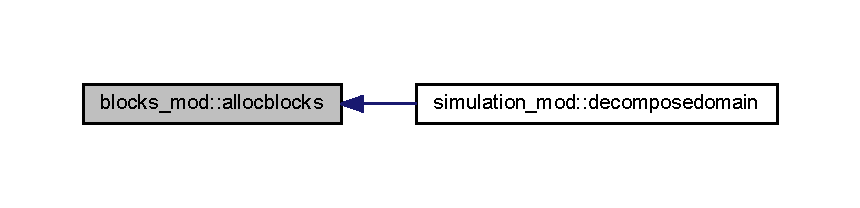
\includegraphics[width=350pt]{namespaceblocks__mod_a639beb0fee2290d46353f4b4702d6711_icgraph}
\end{center}
\end{figure}
\mbox{\Hypertarget{namespaceblocks__mod_a27c7e788c5f3979bfe9d43aad138286a}\label{namespaceblocks__mod_a27c7e788c5f3979bfe9d43aad138286a}} 
\index{blocks\+\_\+mod@{blocks\+\_\+mod}!aottotracers@{aottotracers}}
\index{aottotracers@{aottotracers}!blocks\+\_\+mod@{blocks\+\_\+mod}}
\subsubsection{\texorpdfstring{aottotracers()}{aottotracers()}}
{\footnotesize\ttfamily subroutine blocks\+\_\+mod\+::aottotracers (\begin{DoxyParamCaption}\item[{class(\mbox{\hyperlink{structblocks__mod_1_1block__class}{block\+\_\+class}}), intent(inout)}]{self }\end{DoxyParamCaption})\hspace{0.3cm}{\ttfamily [private]}}



Method to write the data in the AoT back to the Tracer objects in the list. 

\begin{DoxyAuthor}{Author}
Ricardo Birjukovs Canelas -\/ M\+A\+R\+E\+T\+EC 
\end{DoxyAuthor}


Definition at line 305 of file blocks.\+f90.


\begin{DoxyCode}
305     \textcolor{keywordtype}{implicit none}
306     \textcolor{keywordtype}{class}(block\_class), \textcolor{keywordtype}{intent(inout)} :: self
307     \textcolor{keyword}{call }self%AoT%toTracers()
\end{DoxyCode}
\mbox{\Hypertarget{namespaceblocks__mod_a2c3cf5113e1422d812c2c869afde2729}\label{namespaceblocks__mod_a2c3cf5113e1422d812c2c869afde2729}} 
\index{blocks\+\_\+mod@{blocks\+\_\+mod}!callemitter@{callemitter}}
\index{callemitter@{callemitter}!blocks\+\_\+mod@{blocks\+\_\+mod}}
\subsubsection{\texorpdfstring{callemitter()}{callemitter()}}
{\footnotesize\ttfamily subroutine blocks\+\_\+mod\+::callemitter (\begin{DoxyParamCaption}\item[{class(\mbox{\hyperlink{structblocks__mod_1_1block__class}{block\+\_\+class}}), intent(inout)}]{self }\end{DoxyParamCaption})\hspace{0.3cm}{\ttfamily [private]}}



Method to emitt Tracers from currently active Sources on the Block. 

\begin{DoxyAuthor}{Author}
Ricardo Birjukovs Canelas -\/ M\+A\+R\+E\+T\+EC 
\end{DoxyAuthor}


Definition at line 170 of file blocks.\+f90.


\begin{DoxyCode}
170     \textcolor{keywordtype}{implicit none}
171     \textcolor{keywordtype}{class}(block\_class), \textcolor{keywordtype}{intent(inout)} :: self
172     \textcolor{keywordtype}{integer} :: i
173     \textcolor{keywordtype}{class}(*), \textcolor{keywordtype}{pointer} :: aSource
174     \textcolor{keywordtype}{type}(string) :: outext
175     
176     \textcolor{keyword}{call }self%LSource%reset()                   \textcolor{comment}{! reset list iterator}
177     \textcolor{keywordflow}{do} \textcolor{keywordflow}{while}(self%LSource%moreValues())         \textcolor{comment}{! loop while there are values}
178         asource => self%LSource%currentValue()  \textcolor{comment}{! get current value}
179         \textcolor{keywordflow}{select type}(asource)
180 \textcolor{keywordflow}{        class is} (source\_class)
181             \textcolor{keywordflow}{if} (asource%now%active) \textcolor{keywordflow}{then}
182                 asource%now%emission\_stride = asource%now%emission\_stride - 1   \textcolor{comment}{!decreasing the stride at
       this dt}
183                 \textcolor{keywordflow}{if} (asource%now%emission\_stride == 0) \textcolor{keywordflow}{then}                      \textcolor{comment}{!reached the bottom of the
       stride stack, time to emitt}
184                     \textcolor{keyword}{call }self%Emitter%emitt(asource, self%LTracer)
185                     asource%now%emission\_stride = asource%par%emitting\_rate     \textcolor{comment}{!reseting the stride after
       the Source emitts}
186 \textcolor{keywordflow}{                end if}
187 \textcolor{keywordflow}{            end if}
188 \textcolor{keywordflow}{            class default}
189             outext = \textcolor{stringliteral}{'[Block::CallEmitter] Unexepected type of content, not a Source'}
190             \textcolor{keyword}{call }log%put(outext)
191             stop
192 \textcolor{keywordflow}{        end select}
193         \textcolor{keyword}{call }self%LSource%next()            \textcolor{comment}{! increment the list iterator}
194 \textcolor{keywordflow}{    end do}
195     \textcolor{keyword}{call }self%LSource%reset()               \textcolor{comment}{! reset list iterator}
196     
\end{DoxyCode}
\mbox{\Hypertarget{namespaceblocks__mod_a6cc313e046daa2720cbca810d083faa0}\label{namespaceblocks__mod_a6cc313e046daa2720cbca810d083faa0}} 
\index{blocks\+\_\+mod@{blocks\+\_\+mod}!cleanaot@{cleanaot}}
\index{cleanaot@{cleanaot}!blocks\+\_\+mod@{blocks\+\_\+mod}}
\subsubsection{\texorpdfstring{cleanaot()}{cleanaot()}}
{\footnotesize\ttfamily subroutine blocks\+\_\+mod\+::cleanaot (\begin{DoxyParamCaption}\item[{class(\mbox{\hyperlink{structblocks__mod_1_1block__class}{block\+\_\+class}}), intent(inout)}]{self }\end{DoxyParamCaption})\hspace{0.3cm}{\ttfamily [private]}}



Method to clean out the AoT object. 

\begin{DoxyAuthor}{Author}
Ricardo Birjukovs Canelas -\/ M\+A\+R\+E\+T\+EC 
\end{DoxyAuthor}


Definition at line 316 of file blocks.\+f90.


\begin{DoxyCode}
316     \textcolor{keywordtype}{implicit none}
317     \textcolor{keywordtype}{class}(block\_class), \textcolor{keywordtype}{intent(inout)} :: self    
318     \textcolor{keyword}{call }self%AoT%Clean()
\end{DoxyCode}
\mbox{\Hypertarget{namespaceblocks__mod_a25ff530b5125e4cee5b1f474b2491883}\label{namespaceblocks__mod_a25ff530b5125e4cee5b1f474b2491883}} 
\index{blocks\+\_\+mod@{blocks\+\_\+mod}!consolidatearrays@{consolidatearrays}}
\index{consolidatearrays@{consolidatearrays}!blocks\+\_\+mod@{blocks\+\_\+mod}}
\subsubsection{\texorpdfstring{consolidatearrays()}{consolidatearrays()}}
{\footnotesize\ttfamily subroutine blocks\+\_\+mod\+::consolidatearrays (\begin{DoxyParamCaption}\item[{class(\mbox{\hyperlink{structblocks__mod_1_1block__class}{block\+\_\+class}}), intent(inout)}]{self }\end{DoxyParamCaption})\hspace{0.3cm}{\ttfamily [private]}}



Method to clean the Tracer list from inactive Tracers. T\+O\+DO test further optimization. 

\begin{DoxyAuthor}{Author}
Ricardo Birjukovs Canelas -\/ M\+A\+R\+E\+T\+EC 
\end{DoxyAuthor}


Definition at line 245 of file blocks.\+f90.


\begin{DoxyCode}
245     \textcolor{keywordtype}{implicit none}
246     \textcolor{keywordtype}{class}(block\_class), \textcolor{keywordtype}{intent(inout)} :: self
247     \textcolor{keywordtype}{class}(*), \textcolor{keywordtype}{pointer} :: aTracer
248     \textcolor{keywordtype}{type}(string) :: outext
249     \textcolor{keywordtype}{logical} :: notremoved
250     
251     \textcolor{keyword}{call }self%LTracer%reset()                   \textcolor{comment}{! reset list iterator}
252     \textcolor{keywordflow}{do} \textcolor{keywordflow}{while}(self%LTracer%moreValues())         \textcolor{comment}{! loop while there are values}
253         notremoved = .true.
254         atracer => self%LTracer%currentValue()  \textcolor{comment}{! get current value}
255         \textcolor{keywordflow}{select type}(atracer)
256 \textcolor{keywordflow}{        class is} (tracer\_class)
257             \textcolor{keywordflow}{if} (atracer%now%active.eqv. .false.) \textcolor{keywordflow}{then}
258                 \textcolor{keyword}{call }self%LTracer%removeCurrent() \textcolor{comment}{!this advances the iterator to the next position}
259                 notremoved = .false.                
260 \textcolor{keywordflow}{            end if}
261 \textcolor{keywordflow}{            class default}
262             outext = \textcolor{stringliteral}{'[Block::ConsolidateArrays]: Unexepected type of content, not a Tracer'}
263             \textcolor{keyword}{call }log%put(outext)
264             stop
265 \textcolor{keywordflow}{        end select}
266         \textcolor{keywordflow}{if} (notremoved) \textcolor{keyword}{call }self%LTracer%next()    \textcolor{comment}{! increment the list iterator}
267 \textcolor{keywordflow}{    end do}
268     \textcolor{keyword}{call }self%LTracer%reset()                       \textcolor{comment}{! reset list iterator}
269     
\end{DoxyCode}
\mbox{\Hypertarget{namespaceblocks__mod_aa178415bcc40cf169744d356e1a09c6b}\label{namespaceblocks__mod_aa178415bcc40cf169744d356e1a09c6b}} 
\index{blocks\+\_\+mod@{blocks\+\_\+mod}!distributetracers@{distributetracers}}
\index{distributetracers@{distributetracers}!blocks\+\_\+mod@{blocks\+\_\+mod}}
\subsubsection{\texorpdfstring{distributetracers()}{distributetracers()}}
{\footnotesize\ttfamily subroutine blocks\+\_\+mod\+::distributetracers (\begin{DoxyParamCaption}\item[{class(\mbox{\hyperlink{structblocks__mod_1_1block__class}{block\+\_\+class}}), intent(inout)}]{self }\end{DoxyParamCaption})\hspace{0.3cm}{\ttfamily [private]}}



Method to distribute the Tracers to their correct Blocks. 

\begin{DoxyAuthor}{Author}
Ricardo Birjukovs Canelas -\/ M\+A\+R\+E\+T\+EC 
\end{DoxyAuthor}


Definition at line 205 of file blocks.\+f90.


\begin{DoxyCode}
205     \textcolor{keywordtype}{implicit none}
206     \textcolor{keywordtype}{class}(block\_class), \textcolor{keywordtype}{intent(inout)} :: self
207     \textcolor{keywordtype}{integer} :: i, blk
208     \textcolor{keywordtype}{class}(*), \textcolor{keywordtype}{pointer} :: aTracer
209     \textcolor{keywordtype}{type}(string) :: outext
210     \textcolor{keywordtype}{logical} :: notremoved
211     
212     \textcolor{keyword}{call }self%LTracer%reset()                   \textcolor{comment}{! reset list iterator}
213     \textcolor{keywordflow}{do} \textcolor{keywordflow}{while}(self%LTracer%moreValues())         \textcolor{comment}{! loop while there are values}
214         notremoved = .true.
215         atracer => self%LTracer%currentValue()  \textcolor{comment}{! get current value}
216         \textcolor{keywordflow}{select type}(atracer)
217 \textcolor{keywordflow}{        class is} (tracer\_class)
218             \textcolor{keywordflow}{if} (atracer%now%active) \textcolor{keywordflow}{then}
219                 blk = getblockindex(atracer%now%pos)
220                 \textcolor{keywordflow}{if} (blk /= self%id) \textcolor{keywordflow}{then}        \textcolor{comment}{!tracer is on a different block than the current one}
221                     \textcolor{comment}{!PARALLEL this is a CRITICAL section, need to ensure correct tracer index attribution}
222                     \textcolor{keyword}{call }sendtracer(blk,atracer)
223                     \textcolor{keyword}{call }self%LTracer%removeCurrent() \textcolor{comment}{!this also advances the iterator to the next position}
224                     notremoved = .false.
225 \textcolor{keywordflow}{                end if}
226 \textcolor{keywordflow}{            end if}
227 \textcolor{keywordflow}{            class default}
228             outext = \textcolor{stringliteral}{'[Block::DistributeTracers]: Unexepected type of content, not a Tracer'}
229             \textcolor{keyword}{call }log%put(outext)
230             stop
231 \textcolor{keywordflow}{        end select}
232         \textcolor{keywordflow}{if} (notremoved) \textcolor{keyword}{call }self%LTracer%next()    \textcolor{comment}{! increment the list iterator}
233 \textcolor{keywordflow}{    end do}
234     \textcolor{keyword}{call }self%LTracer%reset()                   \textcolor{comment}{! reset list iterator}
235     
\end{DoxyCode}
Here is the call graph for this function\+:\nopagebreak
\begin{figure}[H]
\begin{center}
\leavevmode
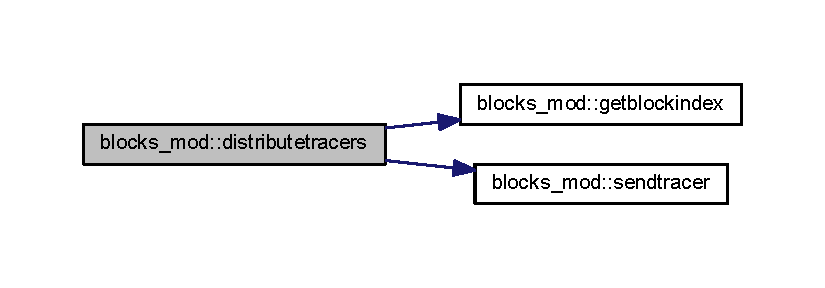
\includegraphics[width=350pt]{namespaceblocks__mod_aa178415bcc40cf169744d356e1a09c6b_cgraph}
\end{center}
\end{figure}
\mbox{\Hypertarget{namespaceblocks__mod_a62e8fb0d6b2535b4499c7a4d848c24ba}\label{namespaceblocks__mod_a62e8fb0d6b2535b4499c7a4d848c24ba}} 
\index{blocks\+\_\+mod@{blocks\+\_\+mod}!getblockindex@{getblockindex}}
\index{getblockindex@{getblockindex}!blocks\+\_\+mod@{blocks\+\_\+mod}}
\subsubsection{\texorpdfstring{getblockindex()}{getblockindex()}}
{\footnotesize\ttfamily integer function, public blocks\+\_\+mod\+::getblockindex (\begin{DoxyParamCaption}\item[{type(vector), intent(in)}]{pt }\end{DoxyParamCaption})}



Returns the index of a Block for a given set of coordinates. 

\begin{DoxyAuthor}{Author}
Ricardo Birjukovs Canelas -\/ M\+A\+R\+E\+T\+EC 
\end{DoxyAuthor}

\begin{DoxyParams}[1]{Parameters}
\mbox{\tt in}  & {\em pt} & \\
\hline
\end{DoxyParams}


Definition at line 342 of file blocks.\+f90.


\begin{DoxyCode}
342     \textcolor{keywordtype}{implicit none}
343     \textcolor{keywordtype}{type}(vector), \textcolor{keywordtype}{intent(in)} :: pt
344     \textcolor{keywordtype}{integer} :: ix, iy, temp
345     \textcolor{keywordtype}{type}(string) :: outext
346     ix = min(int((pt%x + bbox%offset%x)/globals%SimDefs%blocksize%x) + 1, globals%SimDefs%numblocksx)
347     iy = min(int((pt%y + bbox%offset%y)/globals%SimDefs%blocksize%y) + 1, globals%SimDefs%numblocksy)
348     temp = 2*ix + iy -2
349     \textcolor{keywordflow}{if} (temp > globals%SimDefs%numblocks) \textcolor{keywordflow}{then}
350         outext=\textcolor{stringliteral}{'[Blocks::getBlockIndex]: problem in getting correct Block index, stoping'}
351         \textcolor{keyword}{call }log%put(outext)
352         stop
353 \textcolor{keywordflow}{    end if}
354     getblockindex = temp
\end{DoxyCode}
Here is the caller graph for this function\+:\nopagebreak
\begin{figure}[H]
\begin{center}
\leavevmode
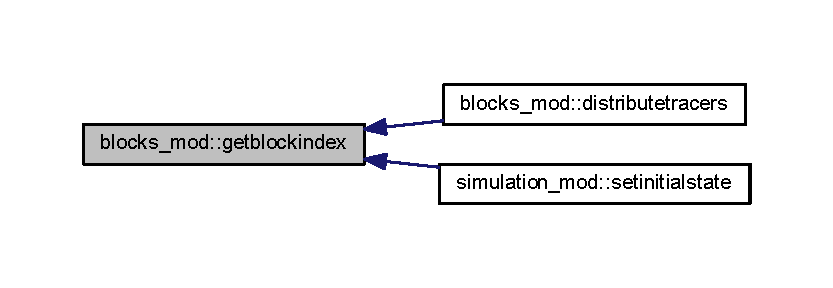
\includegraphics[width=350pt]{namespaceblocks__mod_a62e8fb0d6b2535b4499c7a4d848c24ba_icgraph}
\end{center}
\end{figure}
\mbox{\Hypertarget{namespaceblocks__mod_a534ca69b17b6f54ee07f995b02feff39}\label{namespaceblocks__mod_a534ca69b17b6f54ee07f995b02feff39}} 
\index{blocks\+\_\+mod@{blocks\+\_\+mod}!initblock@{initblock}}
\index{initblock@{initblock}!blocks\+\_\+mod@{blocks\+\_\+mod}}
\subsubsection{\texorpdfstring{initblock()}{initblock()}}
{\footnotesize\ttfamily subroutine blocks\+\_\+mod\+::initblock (\begin{DoxyParamCaption}\item[{class(\mbox{\hyperlink{structblocks__mod_1_1block__class}{block\+\_\+class}}), intent(inout)}]{self,  }\item[{integer, intent(in)}]{id,  }\item[{type(\mbox{\hyperlink{structgeometry__mod_1_1box}{box}}), intent(in)}]{templatebox }\end{DoxyParamCaption})\hspace{0.3cm}{\ttfamily [private]}}



method to allocate and initialize Blocks and their Emitters 

\begin{DoxyAuthor}{Author}
Ricardo Birjukovs Canelas -\/ M\+A\+R\+E\+T\+EC 
\end{DoxyAuthor}

\begin{DoxyParams}[1]{Parameters}
\mbox{\tt in}  & {\em self,id,templatebox} & \\
\hline
\end{DoxyParams}


Definition at line 95 of file blocks.\+f90.


\begin{DoxyCode}
95     \textcolor{keywordtype}{implicit none}
96     \textcolor{keywordtype}{class}(block\_class), \textcolor{keywordtype}{intent(inout)} :: self
97     \textcolor{keywordtype}{integer}, \textcolor{keywordtype}{intent(in)} :: id
98     \textcolor{keywordtype}{type}(box), \textcolor{keywordtype}{intent(in)} :: templatebox
99     \textcolor{keywordtype}{integer} :: sizem, i
100     self%id = id
101     \textcolor{comment}{!setting the block sub-domain}
102     self%extents = templatebox
103     \textcolor{comment}{!initializing the block emitter}
104     \textcolor{keyword}{call }self%Emitter%initialize()
105     \textcolor{comment}{!initializing the block solver}
106     i = globals%Parameters%Integrator
107     \textcolor{keyword}{call }self%Solver%initialize(i, globals%Parameters%IntegratorNames(i))
108     sizem = sizeof(self)
109     \textcolor{keyword}{call }simmemory%addblock(sizem)
\end{DoxyCode}
\mbox{\Hypertarget{namespaceblocks__mod_a7202fad0fdc07ff9111e61e3aa513af9}\label{namespaceblocks__mod_a7202fad0fdc07ff9111e61e3aa513af9}} 
\index{blocks\+\_\+mod@{blocks\+\_\+mod}!numalloctracers@{numalloctracers}}
\index{numalloctracers@{numalloctracers}!blocks\+\_\+mod@{blocks\+\_\+mod}}
\subsubsection{\texorpdfstring{numalloctracers()}{numalloctracers()}}
{\footnotesize\ttfamily integer function blocks\+\_\+mod\+::numalloctracers (\begin{DoxyParamCaption}\item[{class(\mbox{\hyperlink{structblocks__mod_1_1block__class}{block\+\_\+class}}), intent(in)}]{self }\end{DoxyParamCaption})\hspace{0.3cm}{\ttfamily [private]}}



method that returns the total allocated Tracers in the Block 

\begin{DoxyAuthor}{Author}
Ricardo Birjukovs Canelas -\/ M\+A\+R\+E\+T\+EC 
\end{DoxyAuthor}


Definition at line 82 of file blocks.\+f90.


\begin{DoxyCode}
82     \textcolor{keywordtype}{implicit none}
83     \textcolor{keywordtype}{class}(block\_class), \textcolor{keywordtype}{intent(in)} :: self
84     \textcolor{keywordtype}{integer} :: numAllocTracers
85     numalloctracers = self%LTracer%getSize()
\end{DoxyCode}
\mbox{\Hypertarget{namespaceblocks__mod_a6eab8b323cb15dcecb5c6b0c31b4e246}\label{namespaceblocks__mod_a6eab8b323cb15dcecb5c6b0c31b4e246}} 
\index{blocks\+\_\+mod@{blocks\+\_\+mod}!printblock@{printblock}}
\index{printblock@{printblock}!blocks\+\_\+mod@{blocks\+\_\+mod}}
\subsubsection{\texorpdfstring{printblock()}{printblock()}}
{\footnotesize\ttfamily subroutine blocks\+\_\+mod\+::printblock (\begin{DoxyParamCaption}\item[{class(\mbox{\hyperlink{structblocks__mod_1_1block__class}{block\+\_\+class}}), intent(inout)}]{self }\end{DoxyParamCaption})\hspace{0.3cm}{\ttfamily [private]}}



Method to print basic info about the block. 

\begin{DoxyAuthor}{Author}
Ricardo Birjukovs Canelas -\/ M\+A\+R\+E\+T\+EC 
\end{DoxyAuthor}

\begin{DoxyParams}[1]{Parameters}
\mbox{\tt in}  & {\em self} & \\
\hline
\end{DoxyParams}


Definition at line 364 of file blocks.\+f90.


\begin{DoxyCode}
364     \textcolor{keywordtype}{implicit none}
365     \textcolor{keywordtype}{class}(block\_class), \textcolor{keywordtype}{intent(inout)} :: self
366     \textcolor{keywordtype}{type}(string) :: outext, temp\_str
367     temp\_str = self%id
368     outext=\textcolor{stringliteral}{'-->Block '}//temp\_str//\textcolor{stringliteral}{' is a'}
369     \textcolor{keyword}{call }log%put(outext,.false.)
370     \textcolor{keyword}{call }geometry%print(self%extents)
371     temp\_str = self%LSource%getSize()
372     outext=\textcolor{stringliteral}{'      and has '}//temp\_str//\textcolor{stringliteral}{' Sources'}
373     \textcolor{keyword}{call }log%put(outext,.false.)
\end{DoxyCode}
\mbox{\Hypertarget{namespaceblocks__mod_a10f356706988c45a255922fe70851488}\label{namespaceblocks__mod_a10f356706988c45a255922fe70851488}} 
\index{blocks\+\_\+mod@{blocks\+\_\+mod}!printdetailblock@{printdetailblock}}
\index{printdetailblock@{printdetailblock}!blocks\+\_\+mod@{blocks\+\_\+mod}}
\subsubsection{\texorpdfstring{printdetailblock()}{printdetailblock()}}
{\footnotesize\ttfamily subroutine blocks\+\_\+mod\+::printdetailblock (\begin{DoxyParamCaption}\item[{class(\mbox{\hyperlink{structblocks__mod_1_1block__class}{block\+\_\+class}}), intent(inout)}]{self }\end{DoxyParamCaption})\hspace{0.3cm}{\ttfamily [private]}}



Method to print detailed info about the block. 

\begin{DoxyAuthor}{Author}
Ricardo Birjukovs Canelas -\/ M\+A\+R\+E\+T\+EC 
\end{DoxyAuthor}

\begin{DoxyParams}[1]{Parameters}
\mbox{\tt in}  & {\em self} & \\
\hline
\end{DoxyParams}


Definition at line 383 of file blocks.\+f90.


\begin{DoxyCode}
383     \textcolor{keywordtype}{implicit none}
384     \textcolor{keywordtype}{class}(block\_class), \textcolor{keywordtype}{intent(inout)} :: self
385     \textcolor{keywordtype}{type}(string) :: outext, temp\_str
386     \textcolor{keywordtype}{integer} :: i
387     temp\_str = self%id
388     outext=\textcolor{stringliteral}{'-->Block '}//temp\_str//\textcolor{stringliteral}{' is a'}
389     \textcolor{keyword}{call }log%put(outext,.false.)
390     \textcolor{keyword}{call }geometry%print(self%extents)
391     temp\_str = self%LSource%getSize()
392     outext=\textcolor{stringliteral}{'      and has '}//temp\_str//\textcolor{stringliteral}{' Sources'}
393     \textcolor{keyword}{call }log%put(outext,.false.)
394     \textcolor{keyword}{call }self%LSource%print()
\end{DoxyCode}
\mbox{\Hypertarget{namespaceblocks__mod_ae3bd1bfeee831f4b41932839495bb108}\label{namespaceblocks__mod_ae3bd1bfeee831f4b41932839495bb108}} 
\index{blocks\+\_\+mod@{blocks\+\_\+mod}!putsource@{putsource}}
\index{putsource@{putsource}!blocks\+\_\+mod@{blocks\+\_\+mod}}
\subsubsection{\texorpdfstring{putsource()}{putsource()}}
{\footnotesize\ttfamily subroutine blocks\+\_\+mod\+::putsource (\begin{DoxyParamCaption}\item[{class(\mbox{\hyperlink{structblocks__mod_1_1block__class}{block\+\_\+class}}), intent(inout)}]{self,  }\item[{class(\mbox{\hyperlink{structsources__mod_1_1source__class}{source\+\_\+class}}), intent(inout)}]{sourcetoadd }\end{DoxyParamCaption})\hspace{0.3cm}{\ttfamily [private]}}



Method to place a Source on the Block source\+List\+\_\+class object. Adds the Source info to the Block Emitter. 

\begin{DoxyAuthor}{Author}
Ricardo Birjukovs Canelas -\/ M\+A\+R\+E\+T\+EC 
\end{DoxyAuthor}

\begin{DoxyParams}[1]{Parameters}
\mbox{\tt in}  & {\em self,sourcetoadd} & \\
\hline
\mbox{\tt in,out}  & {\em sourcetoadd} & Source object to store \\
\hline
\end{DoxyParams}


Definition at line 120 of file blocks.\+f90.


\begin{DoxyCode}
120     \textcolor{keywordtype}{implicit none}
121     \textcolor{keywordtype}{class}(block\_class), \textcolor{keywordtype}{intent(inout)} :: self
122     \textcolor{keywordtype}{class}(source\_class), \textcolor{keywordtype}{intent(inout)} :: sourcetoadd
123     \textcolor{keyword}{call }self%LSource%add(sourcetoadd)    
124     \textcolor{comment}{!adding this Source to the Block Emitter pool}
125     \textcolor{keyword}{call }self%Emitter%addSource(sourcetoadd)
\end{DoxyCode}
\mbox{\Hypertarget{namespaceblocks__mod_a3245bdadbec6bb123c517921d1503b48}\label{namespaceblocks__mod_a3245bdadbec6bb123c517921d1503b48}} 
\index{blocks\+\_\+mod@{blocks\+\_\+mod}!runsolver@{runsolver}}
\index{runsolver@{runsolver}!blocks\+\_\+mod@{blocks\+\_\+mod}}
\subsubsection{\texorpdfstring{runsolver()}{runsolver()}}
{\footnotesize\ttfamily subroutine blocks\+\_\+mod\+::runsolver (\begin{DoxyParamCaption}\item[{class(\mbox{\hyperlink{structblocks__mod_1_1block__class}{block\+\_\+class}}), intent(inout)}]{self }\end{DoxyParamCaption})\hspace{0.3cm}{\ttfamily [private]}}



Method to run the solver on the data on this Block for the current timestep. Time for some actual numerical work! 

\begin{DoxyAuthor}{Author}
Ricardo Birjukovs Canelas -\/ M\+A\+R\+E\+T\+EC 
\end{DoxyAuthor}


Definition at line 294 of file blocks.\+f90.


\begin{DoxyCode}
294     \textcolor{keywordtype}{implicit none}
295     \textcolor{keywordtype}{class}(block\_class), \textcolor{keywordtype}{intent(inout)} :: self
296     \textcolor{keyword}{call }self%Solver%runStep(self%AoT, self%Background, globals%SimTime, globals%SimDefs%dt)
\end{DoxyCode}
\mbox{\Hypertarget{namespaceblocks__mod_a5a9992de40470e417ec8e40e688f6a0e}\label{namespaceblocks__mod_a5a9992de40470e417ec8e40e688f6a0e}} 
\index{blocks\+\_\+mod@{blocks\+\_\+mod}!sendtracer@{sendtracer}}
\index{sendtracer@{sendtracer}!blocks\+\_\+mod@{blocks\+\_\+mod}}
\subsubsection{\texorpdfstring{sendtracer()}{sendtracer()}}
{\footnotesize\ttfamily subroutine blocks\+\_\+mod\+::sendtracer (\begin{DoxyParamCaption}\item[{integer, intent(in)}]{blk,  }\item[{class($\ast$), intent(in)}]{trc }\end{DoxyParamCaption})\hspace{0.3cm}{\ttfamily [private]}}



Method to send a Tracer from the current Block to another Block. 

\begin{DoxyAuthor}{Author}
Ricardo Birjukovs Canelas -\/ M\+A\+R\+E\+T\+EC 
\end{DoxyAuthor}


Definition at line 327 of file blocks.\+f90.


\begin{DoxyCode}
327     \textcolor{keywordtype}{implicit none}
328     \textcolor{keywordtype}{integer}, \textcolor{keywordtype}{intent(in)} :: blk
329     \textcolor{keywordtype}{class}(*), \textcolor{keywordtype}{intent(in)} :: trc
330     \textcolor{comment}{!PARALLEL this is a CRITICAL section, need to ensure correct tracer}
331     \textcolor{comment}{!index attribution at the new block}
332     \textcolor{keyword}{call }dblock(blk)%LTracer%add(trc)
\end{DoxyCode}
Here is the caller graph for this function\+:\nopagebreak
\begin{figure}[H]
\begin{center}
\leavevmode
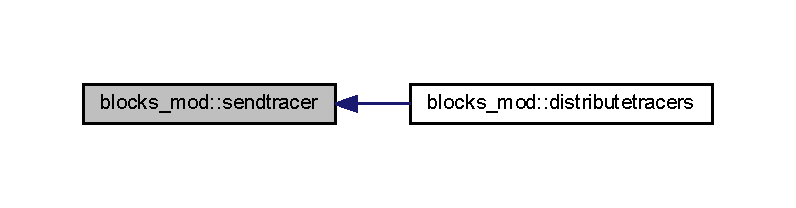
\includegraphics[width=350pt]{namespaceblocks__mod_a5a9992de40470e417ec8e40e688f6a0e_icgraph}
\end{center}
\end{figure}
\mbox{\Hypertarget{namespaceblocks__mod_a8f5a5d9e6cfd16cfd1b179092a204696}\label{namespaceblocks__mod_a8f5a5d9e6cfd16cfd1b179092a204696}} 
\index{blocks\+\_\+mod@{blocks\+\_\+mod}!setblocks@{setblocks}}
\index{setblocks@{setblocks}!blocks\+\_\+mod@{blocks\+\_\+mod}}
\subsubsection{\texorpdfstring{setblocks()}{setblocks()}}
{\footnotesize\ttfamily subroutine, public blocks\+\_\+mod\+::setblocks (\begin{DoxyParamCaption}\item[{logical, intent(in)}]{auto,  }\item[{integer, intent(in)}]{nblk,  }\item[{integer, intent(out)}]{nxi,  }\item[{integer, intent(out)}]{nyi }\end{DoxyParamCaption})}



routine to set the simulation blocks extents and call the block initializer 

\begin{DoxyAuthor}{Author}
Ricardo Birjukovs Canelas -\/ M\+A\+R\+E\+T\+EC 
\end{DoxyAuthor}

\begin{DoxyParams}[1]{Parameters}
\mbox{\tt in}  & {\em auto,nblk,nxi,nyi} & \\
\hline
\end{DoxyParams}


Definition at line 404 of file blocks.\+f90.


\begin{DoxyCode}
404     \textcolor{keywordtype}{implicit none}
405     \textcolor{keywordtype}{logical}, \textcolor{keywordtype}{intent(in)} ::  auto
406     \textcolor{keywordtype}{integer}, \textcolor{keywordtype}{intent(in)} ::  nblk
407     \textcolor{keywordtype}{integer}, \textcolor{keywordtype}{intent(out)} :: nxi, nyi
408     \textcolor{keywordtype}{type}(string) :: outext, temp(2)
409     \textcolor{keywordtype}{integer} :: i, j, b
410     \textcolor{keywordtype}{real(prec)} :: ar
411     \textcolor{keywordtype}{type}(box) :: tempbox
412 
413     \textcolor{keywordflow}{if} (auto) \textcolor{keywordflow}{then}
414         ar = bbox%size%x/bbox%size%y
415         ar = get\_closest\_twopow(ar) \textcolor{comment}{!aspect ratio of our bounding box}
416         nyi = sqrt(nblk/ar)
417         \textcolor{keywordflow}{if} (nyi == 0) \textcolor{keywordflow}{then}
418             temp(1) = ar
419             outext=\textcolor{stringliteral}{'[setBlocks]: block auto sizing failed. Bouding box aspect ratio = '}//temp(1)//\textcolor{stringliteral}{'.
       Stoping'}
420             \textcolor{keyword}{call }log%put(outext)
421             stop
422 \textcolor{keywordflow}{        endif}
423         nxi = (nblk/nyi)
424 
425         b=1
426         \textcolor{keywordflow}{do} i=1, nxi
427             \textcolor{keywordflow}{do} j=1, nyi
428                 tempbox%pt = bbox%pt + bbox%size%x*(i-1)/nxi*ex + bbox%size%y*(j-1)/nyi*ey - bbox%pt%z*ez
429                 tempbox%size = bbox%size%x/nxi*ex + bbox%size%y/nyi*ey
430                 \textcolor{keyword}{call }dblock(b)%initialize(b, tempbox)
431                 b=b+1
432 \textcolor{keywordflow}{            end do}
433 \textcolor{keywordflow}{        end do}
434         temp(1) = nxi
435         temp(2) = nyi
436         outext=\textcolor{stringliteral}{'-->Automatic domain decomposition sucessful. Domain is '}//temp(1)// \textcolor{stringliteral}{' X '} //temp(2)//\textcolor{stringliteral}{'
       Blocks'}
437         \textcolor{keyword}{call }log%put(outext,.false.)
438 \textcolor{keywordflow}{    end if}
439     globals%SimDefs%blocksize = dblock(1)%extents%size
440     \textcolor{comment}{!do i=1, size(DBlock)}
441     \textcolor{comment}{!    call DBlock(i)%print()}
442     \textcolor{comment}{!enddo}
443 
444     \textcolor{keywordflow}{return}
\end{DoxyCode}
Here is the caller graph for this function\+:\nopagebreak
\begin{figure}[H]
\begin{center}
\leavevmode
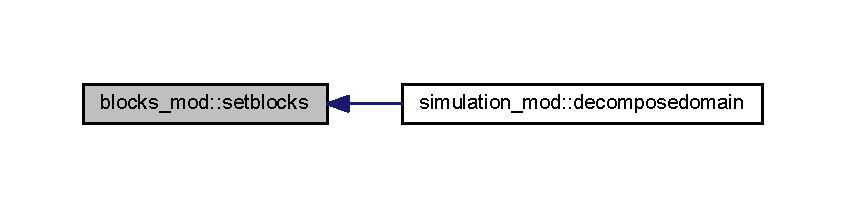
\includegraphics[width=350pt]{namespaceblocks__mod_a8f5a5d9e6cfd16cfd1b179092a204696_icgraph}
\end{center}
\end{figure}
\mbox{\Hypertarget{namespaceblocks__mod_ab9e57cbf0103b632b2b2dfa4e4d4139c}\label{namespaceblocks__mod_ab9e57cbf0103b632b2b2dfa4e4d4139c}} 
\index{blocks\+\_\+mod@{blocks\+\_\+mod}!toogleblocksources@{toogleblocksources}}
\index{toogleblocksources@{toogleblocksources}!blocks\+\_\+mod@{blocks\+\_\+mod}}
\subsubsection{\texorpdfstring{toogleblocksources()}{toogleblocksources()}}
{\footnotesize\ttfamily subroutine blocks\+\_\+mod\+::toogleblocksources (\begin{DoxyParamCaption}\item[{class(\mbox{\hyperlink{structblocks__mod_1_1block__class}{block\+\_\+class}}), intent(inout)}]{self }\end{DoxyParamCaption})\hspace{0.3cm}{\ttfamily [private]}}



Method to activate and deactivate the sources on this block, based on GlobaSim\+Time. 

\begin{DoxyAuthor}{Author}
Ricardo Birjukovs Canelas -\/ M\+A\+R\+E\+T\+EC 
\end{DoxyAuthor}


Definition at line 135 of file blocks.\+f90.


\begin{DoxyCode}
135     \textcolor{keywordtype}{implicit none}
136     \textcolor{keywordtype}{class}(block\_class), \textcolor{keywordtype}{intent(inout)} :: self
137     \textcolor{keywordtype}{integer} :: i
138     \textcolor{keywordtype}{class}(*), \textcolor{keywordtype}{pointer} :: aSource
139     \textcolor{keywordtype}{type}(string) :: outext
140 
141     \textcolor{keyword}{call }self%LSource%reset()                   \textcolor{comment}{! reset list iterator}
142     \textcolor{keywordflow}{do} \textcolor{keywordflow}{while}(self%LSource%moreValues())         \textcolor{comment}{! loop while there are values}
143         asource => self%LSource%currentValue()  \textcolor{comment}{! get current value}
144         \textcolor{keywordflow}{select type}(asource)
145 \textcolor{keywordflow}{        class is} (source\_class)
146             \textcolor{keywordflow}{if} (globals%SimTime <= asource%par%stoptime) \textcolor{keywordflow}{then}       \textcolor{comment}{!SimTime smaller than Source end time}
147                 \textcolor{keywordflow}{if} (globals%SimTime >= asource%par%startime) \textcolor{keywordflow}{then}   \textcolor{comment}{!SimTime larger than source start time}
148                     asource%now%active = .true.
149 \textcolor{keywordflow}{                end if}
150             \textcolor{keywordflow}{else}            \textcolor{comment}{!SimTime larger than Source end time}
151                 asource%now%active = .false.
152 \textcolor{keywordflow}{            end if}
153 \textcolor{keywordflow}{            class default}
154             outext = \textcolor{stringliteral}{'[Block::ToogleBlockSources] Unexepected type of content, not a Source'}
155             \textcolor{keyword}{call }log%put(outext)
156             stop
157 \textcolor{keywordflow}{        end select}
158         \textcolor{keyword}{call }self%LSource%next()            \textcolor{comment}{! increment the list iterator}
159 \textcolor{keywordflow}{    end do}
160     \textcolor{keyword}{call }self%LSource%reset()               \textcolor{comment}{! reset list iterator}
161 
\end{DoxyCode}
\mbox{\Hypertarget{namespaceblocks__mod_ae7afa742f8f89a6a8afdefb7f8c87efd}\label{namespaceblocks__mod_ae7afa742f8f89a6a8afdefb7f8c87efd}} 
\index{blocks\+\_\+mod@{blocks\+\_\+mod}!tracerstoaot@{tracerstoaot}}
\index{tracerstoaot@{tracerstoaot}!blocks\+\_\+mod@{blocks\+\_\+mod}}
\subsubsection{\texorpdfstring{tracerstoaot()}{tracerstoaot()}}
{\footnotesize\ttfamily subroutine blocks\+\_\+mod\+::tracerstoaot (\begin{DoxyParamCaption}\item[{class(\mbox{\hyperlink{structblocks__mod_1_1block__class}{block\+\_\+class}}), intent(inout)}]{self }\end{DoxyParamCaption})\hspace{0.3cm}{\ttfamily [private]}}



Method to build the AoT object at this timestep for actual numerical work. 

\begin{DoxyAuthor}{Author}
Ricardo Birjukovs Canelas -\/ M\+A\+R\+E\+T\+EC 
\end{DoxyAuthor}


Definition at line 278 of file blocks.\+f90.


\begin{DoxyCode}
278     \textcolor{keywordtype}{implicit none}
279     \textcolor{keywordtype}{class}(block\_class), \textcolor{keywordtype}{intent(inout)} :: self
280     self%AoT = aot(self%LTracer)
281     \textcolor{comment}{!if (self%LTracer%getSize() > 0) then}
282     \textcolor{comment}{!    print*, 'From Block ', self%id}
283     \textcolor{comment}{!    call self%AoT%print()}
284     \textcolor{comment}{!end if}
\end{DoxyCode}


\subsection{Variable Documentation}
\mbox{\Hypertarget{namespaceblocks__mod_ac8ad6e3cf7a812f95dadb592336aca50}\label{namespaceblocks__mod_ac8ad6e3cf7a812f95dadb592336aca50}} 
\index{blocks\+\_\+mod@{blocks\+\_\+mod}!dblock@{dblock}}
\index{dblock@{dblock}!blocks\+\_\+mod@{blocks\+\_\+mod}}
\subsubsection{\texorpdfstring{dblock}{dblock}}
{\footnotesize\ttfamily type(\mbox{\hyperlink{structblocks__mod_1_1block__class}{block\+\_\+class}}), dimension(\+:), allocatable, public blocks\+\_\+mod\+::dblock}



Definition at line 67 of file blocks.\+f90.


\begin{DoxyCode}
67     \textcolor{keywordtype}{type}(block\_class), \textcolor{keywordtype}{allocatable}, \textcolor{keywordtype}{dimension(:)} :: DBlock
\end{DoxyCode}

\hypertarget{namespaceboundingbox__mod}{}\section{boundingbox\+\_\+mod Module Reference}
\label{namespaceboundingbox__mod}\index{boundingbox\+\_\+mod@{boundingbox\+\_\+mod}}


Module that defines a simulation Bounding Box.  


\subsection*{Data Types}
\begin{DoxyCompactItemize}
\item 
type \hyperlink{structboundingbox__mod_1_1boundingbox__class}{boundingbox\+\_\+class}
\end{DoxyCompactItemize}
\subsection*{Functions/\+Subroutines}
\begin{DoxyCompactItemize}
\item 
subroutine \hyperlink{namespaceboundingbox__mod_a35e41bb92c19802441dd8d748c3acfb4}{initboundingbox} (self)
\begin{DoxyCompactList}\small\item\em Birjukovs Canelas -\/ M\+A\+R\+E\+T\+EC \end{DoxyCompactList}\item 
subroutine \hyperlink{namespaceboundingbox__mod_a6ec461b758bc180dc72b5fb23169feca}{printboundingbox} (self)
\begin{DoxyCompactList}\small\item\em Birjukovs Canelas -\/ M\+A\+R\+E\+T\+EC \end{DoxyCompactList}\end{DoxyCompactItemize}
\subsection*{Variables}
\begin{DoxyCompactItemize}
\item 
type(\hyperlink{structboundingbox__mod_1_1boundingbox__class}{boundingbox\+\_\+class}), public \hyperlink{namespaceboundingbox__mod_a45e98e492bb546328c98f618a74622ec}{bbox}
\end{DoxyCompactItemize}


\subsection{Detailed Description}
Module that defines a simulation Bounding Box. 

\begin{DoxyAuthor}{Author}
Ricardo Birjukovs Canelas 
\end{DoxyAuthor}


\subsection{Function/\+Subroutine Documentation}
\mbox{\Hypertarget{namespaceboundingbox__mod_a35e41bb92c19802441dd8d748c3acfb4}\label{namespaceboundingbox__mod_a35e41bb92c19802441dd8d748c3acfb4}} 
\index{boundingbox\+\_\+mod@{boundingbox\+\_\+mod}!initboundingbox@{initboundingbox}}
\index{initboundingbox@{initboundingbox}!boundingbox\+\_\+mod@{boundingbox\+\_\+mod}}
\subsubsection{\texorpdfstring{initboundingbox()}{initboundingbox()}}
{\footnotesize\ttfamily subroutine boundingbox\+\_\+mod\+::initboundingbox (\begin{DoxyParamCaption}\item[{class(\hyperlink{structboundingbox__mod_1_1boundingbox__class}{boundingbox\+\_\+class}), intent(inout)}]{self }\end{DoxyParamCaption})\hspace{0.3cm}{\ttfamily [private]}}



Birjukovs Canelas -\/ M\+A\+R\+E\+T\+EC 

Method to initialize the simulation Bounding Box \mbox{\Hypertarget{namespaceboundingbox__mod_a6ec461b758bc180dc72b5fb23169feca}\label{namespaceboundingbox__mod_a6ec461b758bc180dc72b5fb23169feca}} 
\index{boundingbox\+\_\+mod@{boundingbox\+\_\+mod}!printboundingbox@{printboundingbox}}
\index{printboundingbox@{printboundingbox}!boundingbox\+\_\+mod@{boundingbox\+\_\+mod}}
\subsubsection{\texorpdfstring{printboundingbox()}{printboundingbox()}}
{\footnotesize\ttfamily subroutine boundingbox\+\_\+mod\+::printboundingbox (\begin{DoxyParamCaption}\item[{class(\hyperlink{structboundingbox__mod_1_1boundingbox__class}{boundingbox\+\_\+class}), intent(inout)}]{self }\end{DoxyParamCaption})\hspace{0.3cm}{\ttfamily [private]}}



Birjukovs Canelas -\/ M\+A\+R\+E\+T\+EC 

Method to print the simulation Bounding Box 

\subsection{Variable Documentation}
\mbox{\Hypertarget{namespaceboundingbox__mod_a45e98e492bb546328c98f618a74622ec}\label{namespaceboundingbox__mod_a45e98e492bb546328c98f618a74622ec}} 
\index{boundingbox\+\_\+mod@{boundingbox\+\_\+mod}!bbox@{bbox}}
\index{bbox@{bbox}!boundingbox\+\_\+mod@{boundingbox\+\_\+mod}}
\subsubsection{\texorpdfstring{bbox}{bbox}}
{\footnotesize\ttfamily type(\hyperlink{structboundingbox__mod_1_1boundingbox__class}{boundingbox\+\_\+class}), public boundingbox\+\_\+mod\+::bbox}


\hypertarget{namespacecommon__modules}{}\section{common\+\_\+modules Module Reference}
\label{namespacecommon__modules}\index{common\+\_\+modules@{common\+\_\+modules}}


Module to hold all of the commonly used base modules.  




\subsection{Detailed Description}
Module to hold all of the commonly used base modules. 

\begin{DoxyAuthor}{Author}
Ricardo Birjukovs Canelas 
\end{DoxyAuthor}

\hypertarget{namespacecontainer__mod}{}\section{container\+\_\+mod Module Reference}
\label{namespacecontainer__mod}\index{container\+\_\+mod@{container\+\_\+mod}}


Module that defines an unlimited polymorphic container class and related methods. A container is a fundamental entity allowing to build data structures such as lists and arrays.  


\subsection*{Data Types}
\begin{DoxyCompactItemize}
\item 
interface \mbox{\hyperlink{structcontainer__mod_1_1container}{container}}
\end{DoxyCompactItemize}
\subsection*{Functions/\+Subroutines}
\begin{DoxyCompactItemize}
\item 
class($\ast$) function, pointer \mbox{\hyperlink{namespacecontainer__mod_a23a016e747d896622127c0c21dca9836}{getcontent}} (this)
\begin{DoxyCompactList}\small\item\em Method that returns a pointer to the values stored in the container. \end{DoxyCompactList}\item 
subroutine \mbox{\hyperlink{namespacecontainer__mod_ace49cee012b6cd3c41c03556ab0dd884}{storecontent}} (this, to\+\_\+store)
\begin{DoxyCompactList}\small\item\em Method that stores the provided value in the container using sourced allocation. \end{DoxyCompactList}\item 
subroutine \mbox{\hyperlink{namespacecontainer__mod_abf1785185971a527e437d3a489462724}{printcontainer}} (this)
\begin{DoxyCompactList}\small\item\em Method to print the stored value. Only knows about instrinsic types, ignores (but warns) if other types are passed. \end{DoxyCompactList}\item 
class(\mbox{\hyperlink{structcontainer__mod_1_1container}{container}}) function, pointer \mbox{\hyperlink{namespacecontainer__mod_a6262df4ff34024d566cf8261dc20a248}{constructor}} (to\+\_\+store)
\begin{DoxyCompactList}\small\item\em Container constructor, can be used with the \textquotesingle{}container\textquotesingle{} name since it is defined as an interface. \end{DoxyCompactList}\end{DoxyCompactItemize}


\subsection{Detailed Description}
Module that defines an unlimited polymorphic container class and related methods. A container is a fundamental entity allowing to build data structures such as lists and arrays. 

\begin{DoxyAuthor}{Author}
Ricardo Birjukovs Canelas 
\end{DoxyAuthor}


\subsection{Function/\+Subroutine Documentation}
\mbox{\Hypertarget{namespacecontainer__mod_a6262df4ff34024d566cf8261dc20a248}\label{namespacecontainer__mod_a6262df4ff34024d566cf8261dc20a248}} 
\index{container\+\_\+mod@{container\+\_\+mod}!constructor@{constructor}}
\index{constructor@{constructor}!container\+\_\+mod@{container\+\_\+mod}}
\subsubsection{\texorpdfstring{constructor()}{constructor()}}
{\footnotesize\ttfamily class(\mbox{\hyperlink{structcontainer__mod_1_1container}{container}}) function, pointer container\+\_\+mod\+::constructor (\begin{DoxyParamCaption}\item[{class($\ast$), intent(in)}]{to\+\_\+store }\end{DoxyParamCaption})\hspace{0.3cm}{\ttfamily [private]}}



Container constructor, can be used with the \textquotesingle{}container\textquotesingle{} name since it is defined as an interface. 

\begin{DoxyAuthor}{Author}
Ricardo Birjukovs Canelas -\/ M\+A\+R\+E\+T\+EC 
\end{DoxyAuthor}

\begin{DoxyParams}{Parameters}
{\em \mbox{[}to\+\_\+store\mbox{]}} & \\
\hline
\end{DoxyParams}


Definition at line 109 of file container.\+f90.


\begin{DoxyCode}
109     \textcolor{keywordtype}{class}(container), \textcolor{keywordtype}{pointer} :: constructor
110     \textcolor{keywordtype}{class}(*), \textcolor{keywordtype}{intent(in)} :: to\_store
111     \textcolor{keyword}{allocate}(constructor)
112     \textcolor{keyword}{allocate}(constructor%value, source=to\_store)
\end{DoxyCode}
\mbox{\Hypertarget{namespacecontainer__mod_a23a016e747d896622127c0c21dca9836}\label{namespacecontainer__mod_a23a016e747d896622127c0c21dca9836}} 
\index{container\+\_\+mod@{container\+\_\+mod}!getcontent@{getcontent}}
\index{getcontent@{getcontent}!container\+\_\+mod@{container\+\_\+mod}}
\subsubsection{\texorpdfstring{getcontent()}{getcontent()}}
{\footnotesize\ttfamily class($\ast$) function, pointer container\+\_\+mod\+::getcontent (\begin{DoxyParamCaption}\item[{class(\mbox{\hyperlink{structcontainer__mod_1_1container}{container}}), intent(in)}]{this }\end{DoxyParamCaption})\hspace{0.3cm}{\ttfamily [private]}}



Method that returns a pointer to the values stored in the container. 

\begin{DoxyAuthor}{Author}
Ricardo Birjukovs Canelas -\/ M\+A\+R\+E\+T\+EC 
\end{DoxyAuthor}

\begin{DoxyParams}{Parameters}
{\em \mbox{[}this\mbox{]}} & \\
\hline
\end{DoxyParams}


Definition at line 62 of file container.\+f90.


\begin{DoxyCode}
62     \textcolor{keywordtype}{class}(container), \textcolor{keywordtype}{intent(in)} :: this
63     \textcolor{keywordtype}{class}(*), \textcolor{keywordtype}{pointer} :: getContent
64     getcontent => this%value
\end{DoxyCode}
\mbox{\Hypertarget{namespacecontainer__mod_abf1785185971a527e437d3a489462724}\label{namespacecontainer__mod_abf1785185971a527e437d3a489462724}} 
\index{container\+\_\+mod@{container\+\_\+mod}!printcontainer@{printcontainer}}
\index{printcontainer@{printcontainer}!container\+\_\+mod@{container\+\_\+mod}}
\subsubsection{\texorpdfstring{printcontainer()}{printcontainer()}}
{\footnotesize\ttfamily subroutine container\+\_\+mod\+::printcontainer (\begin{DoxyParamCaption}\item[{class(\mbox{\hyperlink{structcontainer__mod_1_1container}{container}}), intent(in)}]{this }\end{DoxyParamCaption})\hspace{0.3cm}{\ttfamily [private]}}



Method to print the stored value. Only knows about instrinsic types, ignores (but warns) if other types are passed. 

\begin{DoxyAuthor}{Author}
Ricardo Birjukovs Canelas -\/ M\+A\+R\+E\+T\+EC 
\end{DoxyAuthor}

\begin{DoxyParams}{Parameters}
{\em \mbox{[}this\mbox{]}} & \\
\hline
\end{DoxyParams}


Definition at line 88 of file container.\+f90.


\begin{DoxyCode}
88     \textcolor{keywordtype}{class}(container), \textcolor{keywordtype}{intent(in)} :: this
89     \textcolor{keywordflow}{select type}(v => this%value)
90 \textcolor{keywordflow}{    type is} (integer)
91         print *, v
92 \textcolor{keywordflow}{    type is} (\textcolor{keywordtype}{character}(*))
93         print *, v(1:1)
94 \textcolor{keywordflow}{    type is} (real)
95         print *, v
96 \textcolor{keywordflow}{        class default}
97         print*, \textcolor{stringliteral}{"[printContainer]: don't know how to print this value, ignoring"}
98 \textcolor{keywordflow}{    end select}
\end{DoxyCode}
\mbox{\Hypertarget{namespacecontainer__mod_ace49cee012b6cd3c41c03556ab0dd884}\label{namespacecontainer__mod_ace49cee012b6cd3c41c03556ab0dd884}} 
\index{container\+\_\+mod@{container\+\_\+mod}!storecontent@{storecontent}}
\index{storecontent@{storecontent}!container\+\_\+mod@{container\+\_\+mod}}
\subsubsection{\texorpdfstring{storecontent()}{storecontent()}}
{\footnotesize\ttfamily subroutine container\+\_\+mod\+::storecontent (\begin{DoxyParamCaption}\item[{class(\mbox{\hyperlink{structcontainer__mod_1_1container}{container}}), intent(inout)}]{this,  }\item[{class($\ast$), intent(in)}]{to\+\_\+store }\end{DoxyParamCaption})\hspace{0.3cm}{\ttfamily [private]}}



Method that stores the provided value in the container using sourced allocation. 

\begin{DoxyAuthor}{Author}
Ricardo Birjukovs Canelas -\/ M\+A\+R\+E\+T\+EC 
\end{DoxyAuthor}

\begin{DoxyParams}{Parameters}
{\em \mbox{[}this,to\+\_\+store\mbox{]}} & \\
\hline
\end{DoxyParams}


Definition at line 75 of file container.\+f90.


\begin{DoxyCode}
75     \textcolor{keywordtype}{class}(container), \textcolor{keywordtype}{intent(inout)} :: this
76     \textcolor{keywordtype}{class}(*), \textcolor{keywordtype}{intent(in)} :: to\_store
77     \textcolor{keyword}{allocate}(this%value, source=to\_store)
\end{DoxyCode}

\hypertarget{namespaceemitter__mod}{}\section{emitter\+\_\+mod Module Reference}
\label{namespaceemitter__mod}\index{emitter\+\_\+mod@{emitter\+\_\+mod}}


Module that defines an emitter class and related methods. This module is responsible for building a potential tracer list based on the availble sources and calling their initializers.  


\subsection*{Data Types}
\begin{DoxyCompactItemize}
\item 
type \hyperlink{structemitter__mod_1_1emitter__class}{emitter\+\_\+class}
\end{DoxyCompactItemize}
\subsection*{Functions/\+Subroutines}
\begin{DoxyCompactItemize}
\item 
subroutine \hyperlink{namespaceemitter__mod_ad89dfc083eae7362441c353225a74ebc}{initracers} (self, srcs)
\begin{DoxyCompactList}\small\item\em method that calls the tracer initialization from the emmiter object \end{DoxyCompactList}\item 
subroutine \hyperlink{namespaceemitter__mod_a7c677125988390e4c57909e4ea82d902}{alloctracers} (self, src)
\begin{DoxyCompactList}\small\item\em method that allocates the tracers respective to a given source \end{DoxyCompactList}\item 
subroutine \hyperlink{namespaceemitter__mod_a6376ad0f8e1739b29caf672aa0750373}{initializeemitter} (self)
\begin{DoxyCompactList}\small\item\em method that initializes an emmiter class object. Sets default values \end{DoxyCompactList}\item 
subroutine \hyperlink{namespaceemitter__mod_ab704fb0e2eb9b3b4b9542706b6fb4eaf}{addsource} (self, src)
\begin{DoxyCompactList}\small\item\em method to compute the total emittable particles per source and allocate them \end{DoxyCompactList}\item 
subroutine \hyperlink{namespaceemitter__mod_a5c219dd6692a761ad4bf968ae750fcc6}{setotalnp} (src)
\begin{DoxyCompactList}\small\item\em private routine that returns the total number of tracers an input source will potentially create \end{DoxyCompactList}\end{DoxyCompactItemize}


\subsection{Detailed Description}
Module that defines an emitter class and related methods. This module is responsible for building a potential tracer list based on the availble sources and calling their initializers. 

\begin{DoxyAuthor}{Author}
Ricardo Birjukovs Canelas 
\end{DoxyAuthor}


\subsection{Function/\+Subroutine Documentation}
\mbox{\Hypertarget{namespaceemitter__mod_ab704fb0e2eb9b3b4b9542706b6fb4eaf}\label{namespaceemitter__mod_ab704fb0e2eb9b3b4b9542706b6fb4eaf}} 
\index{emitter\+\_\+mod@{emitter\+\_\+mod}!addsource@{addsource}}
\index{addsource@{addsource}!emitter\+\_\+mod@{emitter\+\_\+mod}}
\subsubsection{\texorpdfstring{addsource()}{addsource()}}
{\footnotesize\ttfamily subroutine emitter\+\_\+mod\+::addsource (\begin{DoxyParamCaption}\item[{class(\hyperlink{structemitter__mod_1_1emitter__class}{emitter\+\_\+class}), intent(inout)}]{self,  }\item[{class(\hyperlink{structsources__mod_1_1source__class}{source\+\_\+class}), intent(inout)}]{src }\end{DoxyParamCaption})\hspace{0.3cm}{\ttfamily [private]}}



method to compute the total emittable particles per source and allocate them 

\begin{DoxyAuthor}{Author}
Ricardo Birjukovs Canelas -\/ M\+A\+R\+E\+T\+EC 
\end{DoxyAuthor}

\begin{DoxyParams}[1]{Parameters}
\mbox{\tt in}  & {\em self,src} & \\
\hline
\end{DoxyParams}
Here is the call graph for this function\+:\nopagebreak
\begin{figure}[H]
\begin{center}
\leavevmode
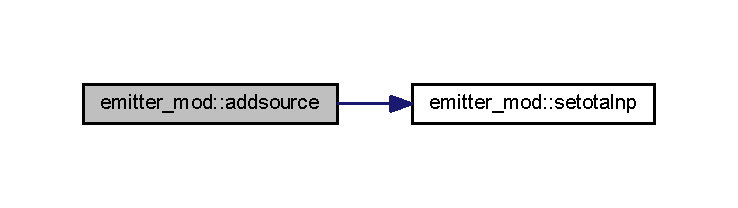
\includegraphics[width=350pt]{namespaceemitter__mod_ab704fb0e2eb9b3b4b9542706b6fb4eaf_cgraph}
\end{center}
\end{figure}
\mbox{\Hypertarget{namespaceemitter__mod_a7c677125988390e4c57909e4ea82d902}\label{namespaceemitter__mod_a7c677125988390e4c57909e4ea82d902}} 
\index{emitter\+\_\+mod@{emitter\+\_\+mod}!alloctracers@{alloctracers}}
\index{alloctracers@{alloctracers}!emitter\+\_\+mod@{emitter\+\_\+mod}}
\subsubsection{\texorpdfstring{alloctracers()}{alloctracers()}}
{\footnotesize\ttfamily subroutine emitter\+\_\+mod\+::alloctracers (\begin{DoxyParamCaption}\item[{class(\hyperlink{structemitter__mod_1_1emitter__class}{emitter\+\_\+class}), intent(inout)}]{self,  }\item[{class(\hyperlink{structsources__mod_1_1source__class}{source\+\_\+class}), intent(inout)}]{src }\end{DoxyParamCaption})\hspace{0.3cm}{\ttfamily [private]}}



method that allocates the tracers respective to a given source 

\begin{DoxyAuthor}{Author}
Ricardo Birjukovs Canelas -\/ M\+A\+R\+E\+T\+EC 
\end{DoxyAuthor}

\begin{DoxyParams}[1]{Parameters}
\mbox{\tt in}  & {\em self,src} & \\
\hline
\end{DoxyParams}
\mbox{\Hypertarget{namespaceemitter__mod_a6376ad0f8e1739b29caf672aa0750373}\label{namespaceemitter__mod_a6376ad0f8e1739b29caf672aa0750373}} 
\index{emitter\+\_\+mod@{emitter\+\_\+mod}!initializeemitter@{initializeemitter}}
\index{initializeemitter@{initializeemitter}!emitter\+\_\+mod@{emitter\+\_\+mod}}
\subsubsection{\texorpdfstring{initializeemitter()}{initializeemitter()}}
{\footnotesize\ttfamily subroutine emitter\+\_\+mod\+::initializeemitter (\begin{DoxyParamCaption}\item[{class(\hyperlink{structemitter__mod_1_1emitter__class}{emitter\+\_\+class}), intent(inout)}]{self }\end{DoxyParamCaption})\hspace{0.3cm}{\ttfamily [private]}}



method that initializes an emmiter class object. Sets default values 

\begin{DoxyAuthor}{Author}
Ricardo Birjukovs Canelas -\/ M\+A\+R\+E\+T\+EC 
\end{DoxyAuthor}

\begin{DoxyParams}[1]{Parameters}
\mbox{\tt in}  & {\em self} & \\
\hline
\end{DoxyParams}
\mbox{\Hypertarget{namespaceemitter__mod_ad89dfc083eae7362441c353225a74ebc}\label{namespaceemitter__mod_ad89dfc083eae7362441c353225a74ebc}} 
\index{emitter\+\_\+mod@{emitter\+\_\+mod}!initracers@{initracers}}
\index{initracers@{initracers}!emitter\+\_\+mod@{emitter\+\_\+mod}}
\subsubsection{\texorpdfstring{initracers()}{initracers()}}
{\footnotesize\ttfamily subroutine emitter\+\_\+mod\+::initracers (\begin{DoxyParamCaption}\item[{class(\hyperlink{structemitter__mod_1_1emitter__class}{emitter\+\_\+class}), intent(inout)}]{self,  }\item[{class(\hyperlink{structsources__mod_1_1source__class}{source\+\_\+class}), dimension(\+:), intent(inout)}]{srcs }\end{DoxyParamCaption})\hspace{0.3cm}{\ttfamily [private]}}



method that calls the tracer initialization from the emmiter object 

\begin{DoxyAuthor}{Author}
Ricardo Birjukovs Canelas -\/ M\+A\+R\+E\+T\+EC 
\end{DoxyAuthor}

\begin{DoxyParams}[1]{Parameters}
\mbox{\tt in}  & {\em self,src} & \\
\hline
\end{DoxyParams}
\mbox{\Hypertarget{namespaceemitter__mod_a5c219dd6692a761ad4bf968ae750fcc6}\label{namespaceemitter__mod_a5c219dd6692a761ad4bf968ae750fcc6}} 
\index{emitter\+\_\+mod@{emitter\+\_\+mod}!setotalnp@{setotalnp}}
\index{setotalnp@{setotalnp}!emitter\+\_\+mod@{emitter\+\_\+mod}}
\subsubsection{\texorpdfstring{setotalnp()}{setotalnp()}}
{\footnotesize\ttfamily subroutine emitter\+\_\+mod\+::setotalnp (\begin{DoxyParamCaption}\item[{class(\hyperlink{structsources__mod_1_1source__class}{source\+\_\+class}), intent(inout)}]{src }\end{DoxyParamCaption})\hspace{0.3cm}{\ttfamily [private]}}



private routine that returns the total number of tracers an input source will potentially create 

\begin{DoxyAuthor}{Author}
Ricardo Birjukovs Canelas -\/ M\+A\+R\+E\+T\+EC 
\end{DoxyAuthor}

\begin{DoxyParams}[1]{Parameters}
\mbox{\tt in}  & {\em src} & \\
\hline
\end{DoxyParams}
${NP}_{total}^{source-i}=(T_{end}^{source-i}-T_{start}^{source-i})*{Rate}^{source-i}*{NP}_{emission}^{source-i}$ Here is the caller graph for this function\+:\nopagebreak
\begin{figure}[H]
\begin{center}
\leavevmode
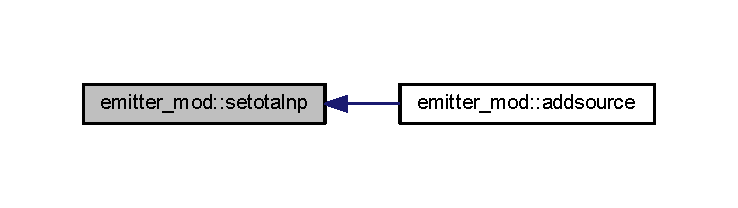
\includegraphics[width=350pt]{namespaceemitter__mod_a5c219dd6692a761ad4bf968ae750fcc6_icgraph}
\end{center}
\end{figure}

\hypertarget{namespacefield__types__mod}{}\section{field\+\_\+types\+\_\+mod Module Reference}
\label{namespacefield__types__mod}\index{field\+\_\+types\+\_\+mod@{field\+\_\+types\+\_\+mod}}


Defines classes for \textquotesingle{}fields\textquotesingle{}\+: 1, 2, 3 and 4D labeled data. Valid for both scalar and vectorial (real) data. Defines a generic wrapper for these classes, that abstracts the user from having to choose their data dimensionality or type to create a field.  


\subsection*{Data Types}
\begin{DoxyCompactItemize}
\item 
type \mbox{\hyperlink{structfield__types__mod_1_1field__class}{field\+\_\+class}}
\item 
type \mbox{\hyperlink{structfield__types__mod_1_1generic__field__class}{generic\+\_\+field\+\_\+class}}
\begin{DoxyCompactList}\small\item\em generic field class. This works as a wrapper for a generic initialization routine. \end{DoxyCompactList}\item 
type \mbox{\hyperlink{structfield__types__mod_1_1scalar1d__field__class}{scalar1d\+\_\+field\+\_\+class}}
\begin{DoxyCompactList}\small\item\em a 1D scalar field class \end{DoxyCompactList}\item 
type \mbox{\hyperlink{structfield__types__mod_1_1scalar2d__field__class}{scalar2d\+\_\+field\+\_\+class}}
\begin{DoxyCompactList}\small\item\em a 2D scalar field class \end{DoxyCompactList}\item 
type \mbox{\hyperlink{structfield__types__mod_1_1scalar3d__field__class}{scalar3d\+\_\+field\+\_\+class}}
\begin{DoxyCompactList}\small\item\em a 3D scalar field class \end{DoxyCompactList}\item 
type \mbox{\hyperlink{structfield__types__mod_1_1scalar4d__field__class}{scalar4d\+\_\+field\+\_\+class}}
\begin{DoxyCompactList}\small\item\em a 4D scalar field class \end{DoxyCompactList}\item 
type \mbox{\hyperlink{structfield__types__mod_1_1scalar__field__class}{scalar\+\_\+field\+\_\+class}}
\begin{DoxyCompactList}\small\item\em a scalar field class \end{DoxyCompactList}\item 
type \mbox{\hyperlink{structfield__types__mod_1_1vectorial2d__field__class}{vectorial2d\+\_\+field\+\_\+class}}
\begin{DoxyCompactList}\small\item\em a 2D vectorial field class \end{DoxyCompactList}\item 
type \mbox{\hyperlink{structfield__types__mod_1_1vectorial3d__field__class}{vectorial3d\+\_\+field\+\_\+class}}
\begin{DoxyCompactList}\small\item\em a 3D vectorial field class \end{DoxyCompactList}\item 
type \mbox{\hyperlink{structfield__types__mod_1_1vectorial4d__field__class}{vectorial4d\+\_\+field\+\_\+class}}
\begin{DoxyCompactList}\small\item\em a 4D vectorial field class \end{DoxyCompactList}\item 
type \mbox{\hyperlink{structfield__types__mod_1_1vectorial__field__class}{vectorial\+\_\+field\+\_\+class}}
\begin{DoxyCompactList}\small\item\em a vectorial field class \end{DoxyCompactList}\end{DoxyCompactItemize}
\subsection*{Functions/\+Subroutines}
\begin{DoxyCompactItemize}
\item 
subroutine \mbox{\hyperlink{namespacefield__types__mod_ae4985a4f37aad76b5bd9d4fdbdec8ff3}{inits1d}} (self, name, units, field)
\begin{DoxyCompactList}\small\item\em Method that allocates and initializes a scalar 1D field in a generic field. \end{DoxyCompactList}\item 
subroutine \mbox{\hyperlink{namespacefield__types__mod_a55a57c6fa8c785a5f529ca577a677845}{inits2d}} (self, name, units, field)
\begin{DoxyCompactList}\small\item\em Method that allocates and initializes a scalar 2D field in a generic field. \end{DoxyCompactList}\item 
subroutine \mbox{\hyperlink{namespacefield__types__mod_ac3c3c9514102272c69299be06deabbcd}{inits3d}} (self, name, units, field)
\begin{DoxyCompactList}\small\item\em Method that allocates and initializes a scalar 3D field in a generic field. \end{DoxyCompactList}\item 
subroutine \mbox{\hyperlink{namespacefield__types__mod_a0499b29bbd4e4628fe73678cf554d918}{inits4d}} (self, name, units, field)
\begin{DoxyCompactList}\small\item\em Method that allocates and initializes a scalar 4D field in a generic field. \end{DoxyCompactList}\item 
subroutine \mbox{\hyperlink{namespacefield__types__mod_a26cb1df2a85bf21d45693942957c9dae}{initv2d}} (self, name, units, field)
\begin{DoxyCompactList}\small\item\em Method that allocates and initializes a vectorial 2D field in a generic field. \end{DoxyCompactList}\item 
subroutine \mbox{\hyperlink{namespacefield__types__mod_ae163912444021fda00f4d821d4c85721}{initv3d}} (self, name, units, field)
\begin{DoxyCompactList}\small\item\em Method that allocates and initializes a vectorial 3D field in a generic field. \end{DoxyCompactList}\item 
subroutine \mbox{\hyperlink{namespacefield__types__mod_a6a387f83b9c3e63a795e3bccfff5573b}{initv4d}} (self, name, units, field)
\begin{DoxyCompactList}\small\item\em Method that allocates and initializes a vectorial 4D field in a generic field. \end{DoxyCompactList}\item 
subroutine \mbox{\hyperlink{namespacefield__types__mod_a40667ebd7c9f62482c267e794a14eff4}{initscalar1dfield}} (self, name, units, dim, field)
\begin{DoxyCompactList}\small\item\em Method that initializes a scalar 1D field. \end{DoxyCompactList}\item 
subroutine \mbox{\hyperlink{namespacefield__types__mod_af0bade94ad526899be6a55a81a407231}{initscalar2dfield}} (self, name, units, dim, field)
\begin{DoxyCompactList}\small\item\em Method that initializes a scalar 2D field. \end{DoxyCompactList}\item 
subroutine \mbox{\hyperlink{namespacefield__types__mod_af27a754aea73132de47e0a1b7168ca2e}{initscalar3dfield}} (self, name, units, dim, field)
\begin{DoxyCompactList}\small\item\em Method that initializes a scalar 3D field. \end{DoxyCompactList}\item 
subroutine \mbox{\hyperlink{namespacefield__types__mod_a52e2310f95a85bf65d4a85427814a5ad}{initscalar4dfield}} (self, name, units, dim, field)
\begin{DoxyCompactList}\small\item\em Method that initializes a scalar 4D field. \end{DoxyCompactList}\item 
subroutine \mbox{\hyperlink{namespacefield__types__mod_a31c78f82114b5bf8014f7aac09030c32}{initvectorial2dfield}} (self, name, units, dim, field)
\begin{DoxyCompactList}\small\item\em Method that initializes a vectorial 2D field. \end{DoxyCompactList}\item 
subroutine \mbox{\hyperlink{namespacefield__types__mod_a712c0d9941013a8f8c28e684a7c7f4c7}{initvectorial3dfield}} (self, name, units, dim, field)
\begin{DoxyCompactList}\small\item\em Method that initializes a vectorial 3D field. \end{DoxyCompactList}\item 
subroutine \mbox{\hyperlink{namespacefield__types__mod_ada2cd66d3baca6f614b2dfb477fc9b3b}{initvectorial4dfield}} (self, name, units, dim, field)
\begin{DoxyCompactList}\small\item\em Method that initializes a vectorial 4D field. \end{DoxyCompactList}\item 
subroutine \mbox{\hyperlink{namespacefield__types__mod_af6090a0e4ff4834c37af5f33d35fa03d}{setfieldmetadata}} (self, name, units, dim)
\begin{DoxyCompactList}\small\item\em Method that initializes a base field object by filling metadata. \end{DoxyCompactList}\item 
subroutine \mbox{\hyperlink{namespacefield__types__mod_a9b7f13b8dea24ec75f1a017a943a3fb5}{printgenericfield}} (self)
\begin{DoxyCompactList}\small\item\em Method that prints the generic field information. \end{DoxyCompactList}\item 
subroutine \mbox{\hyperlink{namespacefield__types__mod_ad1448b34724138b4adf0d0abda0bb012}{test}} (self)
\begin{DoxyCompactList}\small\item\em A class \textquotesingle{}unit\textquotesingle{} test for the \mbox{\hyperlink{structfield__types__mod_1_1generic__field__class}{generic\+\_\+field\+\_\+class}}. \end{DoxyCompactList}\item 
subroutine \mbox{\hyperlink{namespacefield__types__mod_aaf5716bf674e6caa4d8a9f3a14a5b393}{printfield}} (self)
\begin{DoxyCompactList}\small\item\em Method that prints the field information. \end{DoxyCompactList}\item 
type(string) function \mbox{\hyperlink{namespacefield__types__mod_aef22f053fd727cf82be4386d65b47031}{getfieldtype}} (self)
\begin{DoxyCompactList}\small\item\em Method that returns the field type (scalar or vectorial), in a string. \end{DoxyCompactList}\end{DoxyCompactItemize}


\subsection{Detailed Description}
Defines classes for \textquotesingle{}fields\textquotesingle{}\+: 1, 2, 3 and 4D labeled data. Valid for both scalar and vectorial (real) data. Defines a generic wrapper for these classes, that abstracts the user from having to choose their data dimensionality or type to create a field. 

\begin{DoxyAuthor}{Author}
Ricardo Birjukovs Canelas 
\end{DoxyAuthor}


\subsection{Function/\+Subroutine Documentation}
\mbox{\Hypertarget{namespacefield__types__mod_aef22f053fd727cf82be4386d65b47031}\label{namespacefield__types__mod_aef22f053fd727cf82be4386d65b47031}} 
\index{field\+\_\+types\+\_\+mod@{field\+\_\+types\+\_\+mod}!getfieldtype@{getfieldtype}}
\index{getfieldtype@{getfieldtype}!field\+\_\+types\+\_\+mod@{field\+\_\+types\+\_\+mod}}
\subsubsection{\texorpdfstring{getfieldtype()}{getfieldtype()}}
{\footnotesize\ttfamily type(string) function field\+\_\+types\+\_\+mod\+::getfieldtype (\begin{DoxyParamCaption}\item[{class(\mbox{\hyperlink{structfield__types__mod_1_1field__class}{field\+\_\+class}}), intent(in)}]{self }\end{DoxyParamCaption})\hspace{0.3cm}{\ttfamily [private]}}



Method that returns the field type (scalar or vectorial), in a string. 

\begin{DoxyAuthor}{Author}
Ricardo Birjukovs Canelas -\/ M\+A\+R\+E\+T\+EC 
\end{DoxyAuthor}


Definition at line 448 of file fields\+\_\+types.\+f90.


\begin{DoxyCode}
448     \textcolor{keywordtype}{class}(field\_class), \textcolor{keywordtype}{intent(in)} :: self
449     \textcolor{keywordtype}{type}(string) :: getFieldType
450     \textcolor{keywordtype}{type}(string) :: outext
451     \textcolor{keywordflow}{select type}(self)
452 \textcolor{keywordflow}{    class is} (scalar\_field\_class)
453         getfieldtype = \textcolor{stringliteral}{'Scalar'}
454 \textcolor{keywordflow}{    class is} (vectorial\_field\_class)
455         getfieldtype = \textcolor{stringliteral}{'Vectorial'}
456 \textcolor{keywordflow}{        class default}
457         outext = \textcolor{stringliteral}{'[field\_class::getFieldType]: Unexepected type of content, not a scalar or vectorial
       Field'}
458         \textcolor{keyword}{call }log%put(outext)
459         stop
460 \textcolor{keywordflow}{    end select}
\end{DoxyCode}
\mbox{\Hypertarget{namespacefield__types__mod_ae4985a4f37aad76b5bd9d4fdbdec8ff3}\label{namespacefield__types__mod_ae4985a4f37aad76b5bd9d4fdbdec8ff3}} 
\index{field\+\_\+types\+\_\+mod@{field\+\_\+types\+\_\+mod}!inits1d@{inits1d}}
\index{inits1d@{inits1d}!field\+\_\+types\+\_\+mod@{field\+\_\+types\+\_\+mod}}
\subsubsection{\texorpdfstring{inits1d()}{inits1d()}}
{\footnotesize\ttfamily subroutine field\+\_\+types\+\_\+mod\+::inits1d (\begin{DoxyParamCaption}\item[{class(\mbox{\hyperlink{structfield__types__mod_1_1generic__field__class}{generic\+\_\+field\+\_\+class}}), intent(inout)}]{self,  }\item[{type(string), intent(in)}]{name,  }\item[{type(string), intent(in)}]{units,  }\item[{real(prec), dimension(\+:), intent(in)}]{field }\end{DoxyParamCaption})\hspace{0.3cm}{\ttfamily [private]}}



Method that allocates and initializes a scalar 1D field in a generic field. 

\begin{DoxyAuthor}{Author}
Ricardo Birjukovs Canelas -\/ M\+A\+R\+E\+T\+EC 
\end{DoxyAuthor}

\begin{DoxyParams}[1]{Parameters}
\mbox{\tt in}  & {\em self,name,units,field} & \\
\hline
\end{DoxyParams}


Definition at line 134 of file fields\+\_\+types.\+f90.


\begin{DoxyCode}
134     \textcolor{keywordtype}{class}(generic\_field\_class), \textcolor{keywordtype}{intent(inout)} :: self
135     \textcolor{keywordtype}{real(prec)}, \textcolor{keywordtype}{intent(in)}, \textcolor{keywordtype}{dimension(:)} :: field
136     \textcolor{keywordtype}{type}(string), \textcolor{keywordtype}{intent(in)} :: name
137     \textcolor{keywordtype}{type}(string), \textcolor{keywordtype}{intent(in)} :: units
138     \textcolor{keywordflow}{if} (\textcolor{keyword}{allocated}(self%scalar1d%field)) \textcolor{keywordflow}{then}
139         stop \textcolor{stringliteral}{'[generic\_field\_class::initialize]: scalar 1D field already allocated'}
140     \textcolor{keywordflow}{else}
141         \textcolor{keyword}{call }self%scalar1d%initialize(name, units, 1, field)
142 \textcolor{keywordflow}{    end if}
\end{DoxyCode}
Here is the caller graph for this function\+:
\nopagebreak
\begin{figure}[H]
\begin{center}
\leavevmode
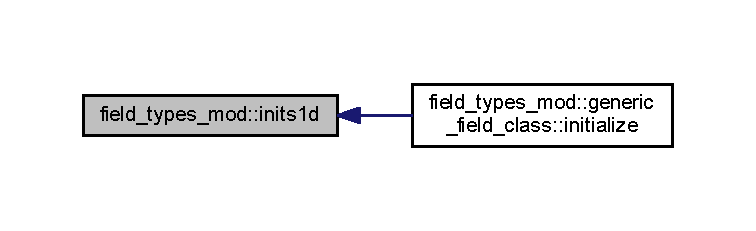
\includegraphics[width=350pt]{namespacefield__types__mod_ae4985a4f37aad76b5bd9d4fdbdec8ff3_icgraph}
\end{center}
\end{figure}
\mbox{\Hypertarget{namespacefield__types__mod_a55a57c6fa8c785a5f529ca577a677845}\label{namespacefield__types__mod_a55a57c6fa8c785a5f529ca577a677845}} 
\index{field\+\_\+types\+\_\+mod@{field\+\_\+types\+\_\+mod}!inits2d@{inits2d}}
\index{inits2d@{inits2d}!field\+\_\+types\+\_\+mod@{field\+\_\+types\+\_\+mod}}
\subsubsection{\texorpdfstring{inits2d()}{inits2d()}}
{\footnotesize\ttfamily subroutine field\+\_\+types\+\_\+mod\+::inits2d (\begin{DoxyParamCaption}\item[{class(\mbox{\hyperlink{structfield__types__mod_1_1generic__field__class}{generic\+\_\+field\+\_\+class}}), intent(inout)}]{self,  }\item[{type(string), intent(in)}]{name,  }\item[{type(string), intent(in)}]{units,  }\item[{real(prec), dimension(\+:,\+:), intent(in)}]{field }\end{DoxyParamCaption})\hspace{0.3cm}{\ttfamily [private]}}



Method that allocates and initializes a scalar 2D field in a generic field. 

\begin{DoxyAuthor}{Author}
Ricardo Birjukovs Canelas -\/ M\+A\+R\+E\+T\+EC 
\end{DoxyAuthor}

\begin{DoxyParams}[1]{Parameters}
\mbox{\tt in}  & {\em self,name,units,field} & \\
\hline
\end{DoxyParams}


Definition at line 152 of file fields\+\_\+types.\+f90.


\begin{DoxyCode}
152     \textcolor{keywordtype}{class}(generic\_field\_class), \textcolor{keywordtype}{intent(inout)} :: self
153     \textcolor{keywordtype}{real(prec)}, \textcolor{keywordtype}{intent(in)}, \textcolor{keywordtype}{dimension(:,:)} :: field
154     \textcolor{keywordtype}{type}(string), \textcolor{keywordtype}{intent(in)} :: name
155     \textcolor{keywordtype}{type}(string), \textcolor{keywordtype}{intent(in)} :: units
156     \textcolor{keywordflow}{if} (\textcolor{keyword}{allocated}(self%scalar2d%field)) \textcolor{keywordflow}{then}
157         stop \textcolor{stringliteral}{'[generic\_field\_class::initialize]: scalar 2D field already allocated'}
158     \textcolor{keywordflow}{else}
159         \textcolor{keyword}{call }self%scalar2d%initialize(name, units, 2, field)
160 \textcolor{keywordflow}{    end if}
\end{DoxyCode}
Here is the caller graph for this function\+:
\nopagebreak
\begin{figure}[H]
\begin{center}
\leavevmode
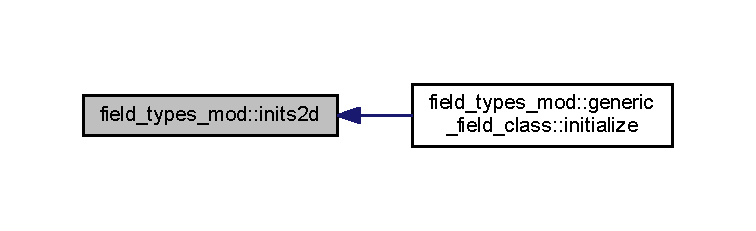
\includegraphics[width=350pt]{namespacefield__types__mod_a55a57c6fa8c785a5f529ca577a677845_icgraph}
\end{center}
\end{figure}
\mbox{\Hypertarget{namespacefield__types__mod_ac3c3c9514102272c69299be06deabbcd}\label{namespacefield__types__mod_ac3c3c9514102272c69299be06deabbcd}} 
\index{field\+\_\+types\+\_\+mod@{field\+\_\+types\+\_\+mod}!inits3d@{inits3d}}
\index{inits3d@{inits3d}!field\+\_\+types\+\_\+mod@{field\+\_\+types\+\_\+mod}}
\subsubsection{\texorpdfstring{inits3d()}{inits3d()}}
{\footnotesize\ttfamily subroutine field\+\_\+types\+\_\+mod\+::inits3d (\begin{DoxyParamCaption}\item[{class(\mbox{\hyperlink{structfield__types__mod_1_1generic__field__class}{generic\+\_\+field\+\_\+class}}), intent(inout)}]{self,  }\item[{type(string), intent(in)}]{name,  }\item[{type(string), intent(in)}]{units,  }\item[{real(prec), dimension(\+:,\+:,\+:), intent(in)}]{field }\end{DoxyParamCaption})\hspace{0.3cm}{\ttfamily [private]}}



Method that allocates and initializes a scalar 3D field in a generic field. 

\begin{DoxyAuthor}{Author}
Ricardo Birjukovs Canelas -\/ M\+A\+R\+E\+T\+EC 
\end{DoxyAuthor}

\begin{DoxyParams}[1]{Parameters}
\mbox{\tt in}  & {\em self,name,units,field} & \\
\hline
\end{DoxyParams}


Definition at line 170 of file fields\+\_\+types.\+f90.


\begin{DoxyCode}
170     \textcolor{keywordtype}{class}(generic\_field\_class), \textcolor{keywordtype}{intent(inout)} :: self
171     \textcolor{keywordtype}{real(prec)}, \textcolor{keywordtype}{intent(in)}, \textcolor{keywordtype}{dimension(:,:,:)} :: field
172     \textcolor{keywordtype}{type}(string), \textcolor{keywordtype}{intent(in)} :: name
173     \textcolor{keywordtype}{type}(string), \textcolor{keywordtype}{intent(in)} :: units
174     \textcolor{keywordflow}{if} (\textcolor{keyword}{allocated}(self%scalar3d%field)) \textcolor{keywordflow}{then}
175         stop \textcolor{stringliteral}{'[generic\_field\_class::initialize]: scalar 3D field already allocated'}
176     \textcolor{keywordflow}{else}
177         \textcolor{keyword}{call }self%scalar3d%initialize(name, units, 3, field)
178 \textcolor{keywordflow}{    end if}
\end{DoxyCode}
Here is the caller graph for this function\+:
\nopagebreak
\begin{figure}[H]
\begin{center}
\leavevmode
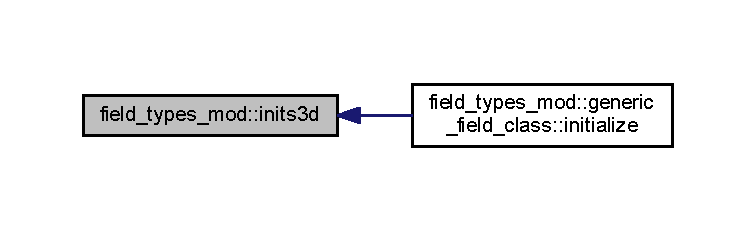
\includegraphics[width=350pt]{namespacefield__types__mod_ac3c3c9514102272c69299be06deabbcd_icgraph}
\end{center}
\end{figure}
\mbox{\Hypertarget{namespacefield__types__mod_a0499b29bbd4e4628fe73678cf554d918}\label{namespacefield__types__mod_a0499b29bbd4e4628fe73678cf554d918}} 
\index{field\+\_\+types\+\_\+mod@{field\+\_\+types\+\_\+mod}!inits4d@{inits4d}}
\index{inits4d@{inits4d}!field\+\_\+types\+\_\+mod@{field\+\_\+types\+\_\+mod}}
\subsubsection{\texorpdfstring{inits4d()}{inits4d()}}
{\footnotesize\ttfamily subroutine field\+\_\+types\+\_\+mod\+::inits4d (\begin{DoxyParamCaption}\item[{class(\mbox{\hyperlink{structfield__types__mod_1_1generic__field__class}{generic\+\_\+field\+\_\+class}}), intent(inout)}]{self,  }\item[{type(string), intent(in)}]{name,  }\item[{type(string), intent(in)}]{units,  }\item[{real(prec), dimension(\+:,\+:,\+:,\+:), intent(in)}]{field }\end{DoxyParamCaption})\hspace{0.3cm}{\ttfamily [private]}}



Method that allocates and initializes a scalar 4D field in a generic field. 

\begin{DoxyAuthor}{Author}
Ricardo Birjukovs Canelas -\/ M\+A\+R\+E\+T\+EC 
\end{DoxyAuthor}

\begin{DoxyParams}[1]{Parameters}
\mbox{\tt in}  & {\em self,name,units,field} & \\
\hline
\end{DoxyParams}


Definition at line 188 of file fields\+\_\+types.\+f90.


\begin{DoxyCode}
188     \textcolor{keywordtype}{class}(generic\_field\_class), \textcolor{keywordtype}{intent(inout)} :: self
189     \textcolor{keywordtype}{real(prec)}, \textcolor{keywordtype}{intent(in)}, \textcolor{keywordtype}{dimension(:,:,:,:)} :: field
190     \textcolor{keywordtype}{type}(string), \textcolor{keywordtype}{intent(in)} :: name
191     \textcolor{keywordtype}{type}(string), \textcolor{keywordtype}{intent(in)} :: units
192     \textcolor{keywordflow}{if} (\textcolor{keyword}{allocated}(self%scalar4d%field)) \textcolor{keywordflow}{then}
193         stop \textcolor{stringliteral}{'[generic\_field\_class::initialize]: scalar 4D field already allocated'}
194     \textcolor{keywordflow}{else}
195         \textcolor{keyword}{call }self%scalar4d%initialize(name, units, 4, field)
196 \textcolor{keywordflow}{    end if}
\end{DoxyCode}
Here is the caller graph for this function\+:
\nopagebreak
\begin{figure}[H]
\begin{center}
\leavevmode
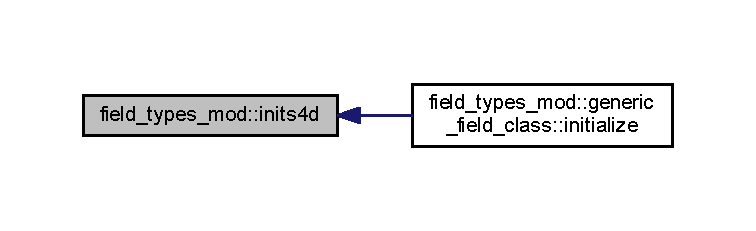
\includegraphics[width=350pt]{namespacefield__types__mod_a0499b29bbd4e4628fe73678cf554d918_icgraph}
\end{center}
\end{figure}
\mbox{\Hypertarget{namespacefield__types__mod_a40667ebd7c9f62482c267e794a14eff4}\label{namespacefield__types__mod_a40667ebd7c9f62482c267e794a14eff4}} 
\index{field\+\_\+types\+\_\+mod@{field\+\_\+types\+\_\+mod}!initscalar1dfield@{initscalar1dfield}}
\index{initscalar1dfield@{initscalar1dfield}!field\+\_\+types\+\_\+mod@{field\+\_\+types\+\_\+mod}}
\subsubsection{\texorpdfstring{initscalar1dfield()}{initscalar1dfield()}}
{\footnotesize\ttfamily subroutine field\+\_\+types\+\_\+mod\+::initscalar1dfield (\begin{DoxyParamCaption}\item[{class(\mbox{\hyperlink{structfield__types__mod_1_1scalar1d__field__class}{scalar1d\+\_\+field\+\_\+class}}), intent(inout)}]{self,  }\item[{type(string), intent(in)}]{name,  }\item[{type(string), intent(in)}]{units,  }\item[{integer, intent(in)}]{dim,  }\item[{real(prec), dimension(\+:), intent(in)}]{field }\end{DoxyParamCaption})\hspace{0.3cm}{\ttfamily [private]}}



Method that initializes a scalar 1D field. 

\begin{DoxyAuthor}{Author}
Ricardo Birjukovs Canelas -\/ M\+A\+R\+E\+T\+EC 
\end{DoxyAuthor}

\begin{DoxyParams}[1]{Parameters}
\mbox{\tt in}  & {\em self,name,units,dim,field} & \\
\hline
\end{DoxyParams}


Definition at line 260 of file fields\+\_\+types.\+f90.


\begin{DoxyCode}
260     \textcolor{keywordtype}{class}(scalar1d\_field\_class), \textcolor{keywordtype}{intent(inout)} :: self
261     \textcolor{keywordtype}{real(prec)}, \textcolor{keywordtype}{intent(in)}, \textcolor{keywordtype}{dimension(:)} :: field
262     \textcolor{keywordtype}{type}(string), \textcolor{keywordtype}{intent(in)} :: name
263     \textcolor{keywordtype}{type}(string), \textcolor{keywordtype}{intent(in)} :: units
264     \textcolor{keywordtype}{integer}, \textcolor{keywordtype}{intent(in)} :: dim
265     \textcolor{keyword}{call }self%setFieldMetadata(name, units, dim)
266     \textcolor{keyword}{allocate}(self%field, source = field)
\end{DoxyCode}
\mbox{\Hypertarget{namespacefield__types__mod_af0bade94ad526899be6a55a81a407231}\label{namespacefield__types__mod_af0bade94ad526899be6a55a81a407231}} 
\index{field\+\_\+types\+\_\+mod@{field\+\_\+types\+\_\+mod}!initscalar2dfield@{initscalar2dfield}}
\index{initscalar2dfield@{initscalar2dfield}!field\+\_\+types\+\_\+mod@{field\+\_\+types\+\_\+mod}}
\subsubsection{\texorpdfstring{initscalar2dfield()}{initscalar2dfield()}}
{\footnotesize\ttfamily subroutine field\+\_\+types\+\_\+mod\+::initscalar2dfield (\begin{DoxyParamCaption}\item[{class(\mbox{\hyperlink{structfield__types__mod_1_1scalar2d__field__class}{scalar2d\+\_\+field\+\_\+class}}), intent(inout)}]{self,  }\item[{type(string), intent(in)}]{name,  }\item[{type(string), intent(in)}]{units,  }\item[{integer, intent(in)}]{dim,  }\item[{real(prec), dimension(\+:,\+:), intent(in)}]{field }\end{DoxyParamCaption})\hspace{0.3cm}{\ttfamily [private]}}



Method that initializes a scalar 2D field. 

\begin{DoxyAuthor}{Author}
Ricardo Birjukovs Canelas -\/ M\+A\+R\+E\+T\+EC 
\end{DoxyAuthor}

\begin{DoxyParams}[1]{Parameters}
\mbox{\tt in}  & {\em self,name,units,dim,field} & \\
\hline
\end{DoxyParams}


Definition at line 276 of file fields\+\_\+types.\+f90.


\begin{DoxyCode}
276     \textcolor{keywordtype}{class}(scalar2d\_field\_class), \textcolor{keywordtype}{intent(inout)} :: self
277     \textcolor{keywordtype}{real(prec)}, \textcolor{keywordtype}{intent(in)}, \textcolor{keywordtype}{dimension(:,:)} :: field
278     \textcolor{keywordtype}{type}(string), \textcolor{keywordtype}{intent(in)} :: name
279     \textcolor{keywordtype}{type}(string), \textcolor{keywordtype}{intent(in)} :: units
280     \textcolor{keywordtype}{integer}, \textcolor{keywordtype}{intent(in)} :: dim
281     \textcolor{keyword}{call }self%setFieldMetadata(name, units, dim)
282     \textcolor{keyword}{allocate}(self%field, source = field)
\end{DoxyCode}
\mbox{\Hypertarget{namespacefield__types__mod_af27a754aea73132de47e0a1b7168ca2e}\label{namespacefield__types__mod_af27a754aea73132de47e0a1b7168ca2e}} 
\index{field\+\_\+types\+\_\+mod@{field\+\_\+types\+\_\+mod}!initscalar3dfield@{initscalar3dfield}}
\index{initscalar3dfield@{initscalar3dfield}!field\+\_\+types\+\_\+mod@{field\+\_\+types\+\_\+mod}}
\subsubsection{\texorpdfstring{initscalar3dfield()}{initscalar3dfield()}}
{\footnotesize\ttfamily subroutine field\+\_\+types\+\_\+mod\+::initscalar3dfield (\begin{DoxyParamCaption}\item[{class(\mbox{\hyperlink{structfield__types__mod_1_1scalar3d__field__class}{scalar3d\+\_\+field\+\_\+class}}), intent(inout)}]{self,  }\item[{type(string), intent(in)}]{name,  }\item[{type(string), intent(in)}]{units,  }\item[{integer, intent(in)}]{dim,  }\item[{real(prec), dimension(\+:,\+:,\+:), intent(in)}]{field }\end{DoxyParamCaption})\hspace{0.3cm}{\ttfamily [private]}}



Method that initializes a scalar 3D field. 

\begin{DoxyAuthor}{Author}
Ricardo Birjukovs Canelas -\/ M\+A\+R\+E\+T\+EC 
\end{DoxyAuthor}

\begin{DoxyParams}[1]{Parameters}
\mbox{\tt in}  & {\em self,name,units,dim,field} & \\
\hline
\end{DoxyParams}


Definition at line 292 of file fields\+\_\+types.\+f90.


\begin{DoxyCode}
292     \textcolor{keywordtype}{class}(scalar3d\_field\_class), \textcolor{keywordtype}{intent(inout)} :: self
293     \textcolor{keywordtype}{real(prec)}, \textcolor{keywordtype}{intent(in)}, \textcolor{keywordtype}{dimension(:,:,:)} :: field
294     \textcolor{keywordtype}{type}(string), \textcolor{keywordtype}{intent(in)} :: name
295     \textcolor{keywordtype}{type}(string), \textcolor{keywordtype}{intent(in)} :: units
296     \textcolor{keywordtype}{integer}, \textcolor{keywordtype}{intent(in)} :: dim
297     \textcolor{keyword}{call }self%setFieldMetadata(name, units, dim)
298     \textcolor{keyword}{allocate}(self%field, source = field)
\end{DoxyCode}
\mbox{\Hypertarget{namespacefield__types__mod_a52e2310f95a85bf65d4a85427814a5ad}\label{namespacefield__types__mod_a52e2310f95a85bf65d4a85427814a5ad}} 
\index{field\+\_\+types\+\_\+mod@{field\+\_\+types\+\_\+mod}!initscalar4dfield@{initscalar4dfield}}
\index{initscalar4dfield@{initscalar4dfield}!field\+\_\+types\+\_\+mod@{field\+\_\+types\+\_\+mod}}
\subsubsection{\texorpdfstring{initscalar4dfield()}{initscalar4dfield()}}
{\footnotesize\ttfamily subroutine field\+\_\+types\+\_\+mod\+::initscalar4dfield (\begin{DoxyParamCaption}\item[{class(\mbox{\hyperlink{structfield__types__mod_1_1scalar4d__field__class}{scalar4d\+\_\+field\+\_\+class}}), intent(inout)}]{self,  }\item[{type(string), intent(in)}]{name,  }\item[{type(string), intent(in)}]{units,  }\item[{integer, intent(in)}]{dim,  }\item[{real(prec), dimension(\+:,\+:,\+:,\+:), intent(in)}]{field }\end{DoxyParamCaption})\hspace{0.3cm}{\ttfamily [private]}}



Method that initializes a scalar 4D field. 

\begin{DoxyAuthor}{Author}
Ricardo Birjukovs Canelas -\/ M\+A\+R\+E\+T\+EC 
\end{DoxyAuthor}

\begin{DoxyParams}[1]{Parameters}
\mbox{\tt in}  & {\em self,name,units,dim,field} & \\
\hline
\end{DoxyParams}


Definition at line 308 of file fields\+\_\+types.\+f90.


\begin{DoxyCode}
308     \textcolor{keywordtype}{class}(scalar4d\_field\_class), \textcolor{keywordtype}{intent(inout)} :: self
309     \textcolor{keywordtype}{real(prec)}, \textcolor{keywordtype}{intent(in)}, \textcolor{keywordtype}{dimension(:,:,:,:)} :: field
310     \textcolor{keywordtype}{type}(string), \textcolor{keywordtype}{intent(in)} :: name
311     \textcolor{keywordtype}{type}(string), \textcolor{keywordtype}{intent(in)} :: units
312     \textcolor{keywordtype}{integer}, \textcolor{keywordtype}{intent(in)} :: dim
313     \textcolor{keyword}{call }self%setFieldMetadata(name, units, dim)
314     \textcolor{keyword}{allocate}(self%field, source = field)
\end{DoxyCode}
\mbox{\Hypertarget{namespacefield__types__mod_a26cb1df2a85bf21d45693942957c9dae}\label{namespacefield__types__mod_a26cb1df2a85bf21d45693942957c9dae}} 
\index{field\+\_\+types\+\_\+mod@{field\+\_\+types\+\_\+mod}!initv2d@{initv2d}}
\index{initv2d@{initv2d}!field\+\_\+types\+\_\+mod@{field\+\_\+types\+\_\+mod}}
\subsubsection{\texorpdfstring{initv2d()}{initv2d()}}
{\footnotesize\ttfamily subroutine field\+\_\+types\+\_\+mod\+::initv2d (\begin{DoxyParamCaption}\item[{class(\mbox{\hyperlink{structfield__types__mod_1_1generic__field__class}{generic\+\_\+field\+\_\+class}}), intent(inout)}]{self,  }\item[{type(string), intent(in)}]{name,  }\item[{type(string), intent(in)}]{units,  }\item[{type(vector), dimension(\+:,\+:), intent(in)}]{field }\end{DoxyParamCaption})\hspace{0.3cm}{\ttfamily [private]}}



Method that allocates and initializes a vectorial 2D field in a generic field. 

\begin{DoxyAuthor}{Author}
Ricardo Birjukovs Canelas -\/ M\+A\+R\+E\+T\+EC 
\end{DoxyAuthor}

\begin{DoxyParams}[1]{Parameters}
\mbox{\tt in}  & {\em self,name,units,field} & \\
\hline
\end{DoxyParams}


Definition at line 206 of file fields\+\_\+types.\+f90.


\begin{DoxyCode}
206     \textcolor{keywordtype}{class}(generic\_field\_class), \textcolor{keywordtype}{intent(inout)} :: self
207     \textcolor{keywordtype}{type}(vector), \textcolor{keywordtype}{intent(in)}, \textcolor{keywordtype}{dimension(:,:)} :: field
208     \textcolor{keywordtype}{type}(string), \textcolor{keywordtype}{intent(in)} :: name
209     \textcolor{keywordtype}{type}(string), \textcolor{keywordtype}{intent(in)} :: units
210     \textcolor{keywordflow}{if} (\textcolor{keyword}{allocated}(self%vectorial2d%field)) \textcolor{keywordflow}{then}
211         stop \textcolor{stringliteral}{'[generic\_field\_class::initialize]: vectorial 2D field already allocated'}
212     \textcolor{keywordflow}{else}
213         \textcolor{keyword}{call }self%vectorial2d%initialize(name, units, 2, field)
214 \textcolor{keywordflow}{    end if}
\end{DoxyCode}
Here is the caller graph for this function\+:
\nopagebreak
\begin{figure}[H]
\begin{center}
\leavevmode
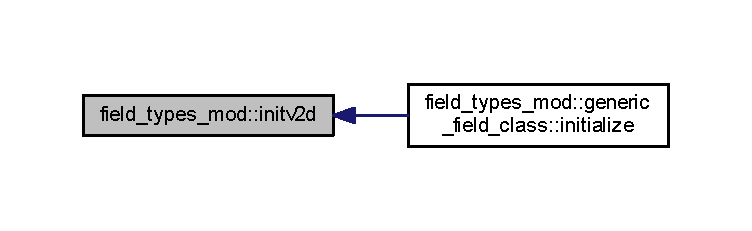
\includegraphics[width=350pt]{namespacefield__types__mod_a26cb1df2a85bf21d45693942957c9dae_icgraph}
\end{center}
\end{figure}
\mbox{\Hypertarget{namespacefield__types__mod_ae163912444021fda00f4d821d4c85721}\label{namespacefield__types__mod_ae163912444021fda00f4d821d4c85721}} 
\index{field\+\_\+types\+\_\+mod@{field\+\_\+types\+\_\+mod}!initv3d@{initv3d}}
\index{initv3d@{initv3d}!field\+\_\+types\+\_\+mod@{field\+\_\+types\+\_\+mod}}
\subsubsection{\texorpdfstring{initv3d()}{initv3d()}}
{\footnotesize\ttfamily subroutine field\+\_\+types\+\_\+mod\+::initv3d (\begin{DoxyParamCaption}\item[{class(\mbox{\hyperlink{structfield__types__mod_1_1generic__field__class}{generic\+\_\+field\+\_\+class}}), intent(inout)}]{self,  }\item[{type(string), intent(in)}]{name,  }\item[{type(string), intent(in)}]{units,  }\item[{type(vector), dimension(\+:,\+:,\+:), intent(in)}]{field }\end{DoxyParamCaption})\hspace{0.3cm}{\ttfamily [private]}}



Method that allocates and initializes a vectorial 3D field in a generic field. 

\begin{DoxyAuthor}{Author}
Ricardo Birjukovs Canelas -\/ M\+A\+R\+E\+T\+EC 
\end{DoxyAuthor}

\begin{DoxyParams}[1]{Parameters}
\mbox{\tt in}  & {\em self,name,units,field} & \\
\hline
\end{DoxyParams}


Definition at line 224 of file fields\+\_\+types.\+f90.


\begin{DoxyCode}
224     \textcolor{keywordtype}{class}(generic\_field\_class), \textcolor{keywordtype}{intent(inout)} :: self
225     \textcolor{keywordtype}{type}(vector), \textcolor{keywordtype}{intent(in)}, \textcolor{keywordtype}{dimension(:,:,:)} :: field
226     \textcolor{keywordtype}{type}(string), \textcolor{keywordtype}{intent(in)} :: name
227     \textcolor{keywordtype}{type}(string), \textcolor{keywordtype}{intent(in)} :: units
228     \textcolor{keywordflow}{if} (\textcolor{keyword}{allocated}(self%vectorial3d%field)) \textcolor{keywordflow}{then}
229         stop \textcolor{stringliteral}{'[generic\_field\_class::initialize]: vectorial 3D field already allocated'}
230     \textcolor{keywordflow}{else}
231         \textcolor{keyword}{call }self%vectorial3d%initialize(name, units, 3, field)
232 \textcolor{keywordflow}{    end if}
\end{DoxyCode}
Here is the caller graph for this function\+:
\nopagebreak
\begin{figure}[H]
\begin{center}
\leavevmode
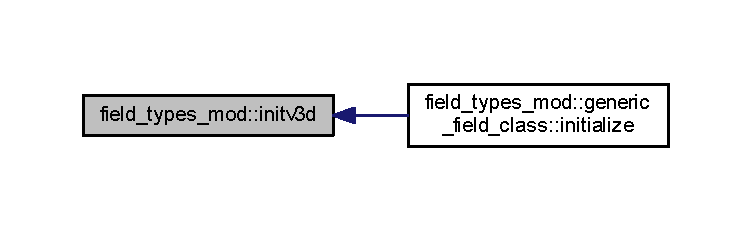
\includegraphics[width=350pt]{namespacefield__types__mod_ae163912444021fda00f4d821d4c85721_icgraph}
\end{center}
\end{figure}
\mbox{\Hypertarget{namespacefield__types__mod_a6a387f83b9c3e63a795e3bccfff5573b}\label{namespacefield__types__mod_a6a387f83b9c3e63a795e3bccfff5573b}} 
\index{field\+\_\+types\+\_\+mod@{field\+\_\+types\+\_\+mod}!initv4d@{initv4d}}
\index{initv4d@{initv4d}!field\+\_\+types\+\_\+mod@{field\+\_\+types\+\_\+mod}}
\subsubsection{\texorpdfstring{initv4d()}{initv4d()}}
{\footnotesize\ttfamily subroutine field\+\_\+types\+\_\+mod\+::initv4d (\begin{DoxyParamCaption}\item[{class(\mbox{\hyperlink{structfield__types__mod_1_1generic__field__class}{generic\+\_\+field\+\_\+class}}), intent(inout)}]{self,  }\item[{type(string), intent(in)}]{name,  }\item[{type(string), intent(in)}]{units,  }\item[{type(vector), dimension(\+:,\+:,\+:,\+:), intent(in)}]{field }\end{DoxyParamCaption})\hspace{0.3cm}{\ttfamily [private]}}



Method that allocates and initializes a vectorial 4D field in a generic field. 

\begin{DoxyAuthor}{Author}
Ricardo Birjukovs Canelas -\/ M\+A\+R\+E\+T\+EC 
\end{DoxyAuthor}

\begin{DoxyParams}[1]{Parameters}
\mbox{\tt in}  & {\em self,name,units,field} & \\
\hline
\end{DoxyParams}


Definition at line 242 of file fields\+\_\+types.\+f90.


\begin{DoxyCode}
242     \textcolor{keywordtype}{class}(generic\_field\_class), \textcolor{keywordtype}{intent(inout)} :: self
243     \textcolor{keywordtype}{type}(vector), \textcolor{keywordtype}{intent(in)}, \textcolor{keywordtype}{dimension(:,:,:,:)} :: field
244     \textcolor{keywordtype}{type}(string), \textcolor{keywordtype}{intent(in)} :: name
245     \textcolor{keywordtype}{type}(string), \textcolor{keywordtype}{intent(in)} :: units
246     \textcolor{keywordflow}{if} (\textcolor{keyword}{allocated}(self%vectorial4d%field)) \textcolor{keywordflow}{then}
247         stop \textcolor{stringliteral}{'[generic\_field\_class::initialize]: vectorial 4D field already allocated'}
248     \textcolor{keywordflow}{else}
249         \textcolor{keyword}{call }self%vectorial4d%initialize(name, units, 4, field)
250 \textcolor{keywordflow}{    end if}
\end{DoxyCode}
Here is the caller graph for this function\+:
\nopagebreak
\begin{figure}[H]
\begin{center}
\leavevmode
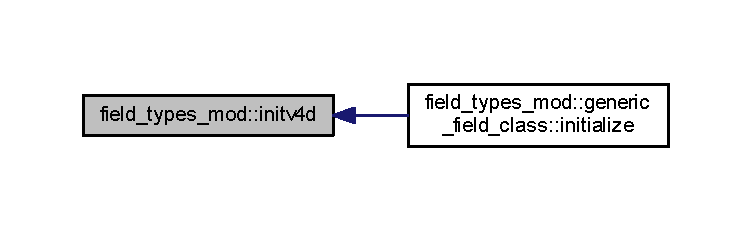
\includegraphics[width=350pt]{namespacefield__types__mod_a6a387f83b9c3e63a795e3bccfff5573b_icgraph}
\end{center}
\end{figure}
\mbox{\Hypertarget{namespacefield__types__mod_a31c78f82114b5bf8014f7aac09030c32}\label{namespacefield__types__mod_a31c78f82114b5bf8014f7aac09030c32}} 
\index{field\+\_\+types\+\_\+mod@{field\+\_\+types\+\_\+mod}!initvectorial2dfield@{initvectorial2dfield}}
\index{initvectorial2dfield@{initvectorial2dfield}!field\+\_\+types\+\_\+mod@{field\+\_\+types\+\_\+mod}}
\subsubsection{\texorpdfstring{initvectorial2dfield()}{initvectorial2dfield()}}
{\footnotesize\ttfamily subroutine field\+\_\+types\+\_\+mod\+::initvectorial2dfield (\begin{DoxyParamCaption}\item[{class(\mbox{\hyperlink{structfield__types__mod_1_1vectorial2d__field__class}{vectorial2d\+\_\+field\+\_\+class}}), intent(inout)}]{self,  }\item[{type(string), intent(in)}]{name,  }\item[{type(string), intent(in)}]{units,  }\item[{integer, intent(in)}]{dim,  }\item[{type(vector), dimension(\+:,\+:), intent(in)}]{field }\end{DoxyParamCaption})\hspace{0.3cm}{\ttfamily [private]}}



Method that initializes a vectorial 2D field. 

\begin{DoxyAuthor}{Author}
Ricardo Birjukovs Canelas -\/ M\+A\+R\+E\+T\+EC 
\end{DoxyAuthor}

\begin{DoxyParams}[1]{Parameters}
\mbox{\tt in}  & {\em self,name,units,dim,field} & \\
\hline
\end{DoxyParams}


Definition at line 324 of file fields\+\_\+types.\+f90.


\begin{DoxyCode}
324     \textcolor{keywordtype}{class}(vectorial2d\_field\_class), \textcolor{keywordtype}{intent(inout)} :: self
325     \textcolor{keywordtype}{type}(vector), \textcolor{keywordtype}{intent(in)}, \textcolor{keywordtype}{dimension(:,:)} :: field
326     \textcolor{keywordtype}{type}(string), \textcolor{keywordtype}{intent(in)} :: name
327     \textcolor{keywordtype}{type}(string), \textcolor{keywordtype}{intent(in)} :: units
328     \textcolor{keywordtype}{integer}, \textcolor{keywordtype}{intent(in)} :: dim
329     \textcolor{keyword}{call }self%setFieldMetadata(name, units, dim)
330     \textcolor{keyword}{allocate}(self%field, source = field)
\end{DoxyCode}
\mbox{\Hypertarget{namespacefield__types__mod_a712c0d9941013a8f8c28e684a7c7f4c7}\label{namespacefield__types__mod_a712c0d9941013a8f8c28e684a7c7f4c7}} 
\index{field\+\_\+types\+\_\+mod@{field\+\_\+types\+\_\+mod}!initvectorial3dfield@{initvectorial3dfield}}
\index{initvectorial3dfield@{initvectorial3dfield}!field\+\_\+types\+\_\+mod@{field\+\_\+types\+\_\+mod}}
\subsubsection{\texorpdfstring{initvectorial3dfield()}{initvectorial3dfield()}}
{\footnotesize\ttfamily subroutine field\+\_\+types\+\_\+mod\+::initvectorial3dfield (\begin{DoxyParamCaption}\item[{class(\mbox{\hyperlink{structfield__types__mod_1_1vectorial3d__field__class}{vectorial3d\+\_\+field\+\_\+class}}), intent(inout)}]{self,  }\item[{type(string), intent(in)}]{name,  }\item[{type(string), intent(in)}]{units,  }\item[{integer, intent(in)}]{dim,  }\item[{type(vector), dimension(\+:,\+:,\+:), intent(in)}]{field }\end{DoxyParamCaption})\hspace{0.3cm}{\ttfamily [private]}}



Method that initializes a vectorial 3D field. 

\begin{DoxyAuthor}{Author}
Ricardo Birjukovs Canelas -\/ M\+A\+R\+E\+T\+EC 
\end{DoxyAuthor}

\begin{DoxyParams}[1]{Parameters}
\mbox{\tt in}  & {\em self,name,units,dim,field} & \\
\hline
\end{DoxyParams}


Definition at line 340 of file fields\+\_\+types.\+f90.


\begin{DoxyCode}
340     \textcolor{keywordtype}{class}(vectorial3d\_field\_class), \textcolor{keywordtype}{intent(inout)} :: self
341     \textcolor{keywordtype}{type}(vector), \textcolor{keywordtype}{intent(in)}, \textcolor{keywordtype}{dimension(:,:,:)} :: field
342     \textcolor{keywordtype}{type}(string), \textcolor{keywordtype}{intent(in)} :: name
343     \textcolor{keywordtype}{type}(string), \textcolor{keywordtype}{intent(in)} :: units
344     \textcolor{keywordtype}{integer}, \textcolor{keywordtype}{intent(in)} :: dim
345     \textcolor{keyword}{call }self%setFieldMetadata(name, units, dim)
346     \textcolor{keyword}{allocate}(self%field, source = field)
\end{DoxyCode}
\mbox{\Hypertarget{namespacefield__types__mod_ada2cd66d3baca6f614b2dfb477fc9b3b}\label{namespacefield__types__mod_ada2cd66d3baca6f614b2dfb477fc9b3b}} 
\index{field\+\_\+types\+\_\+mod@{field\+\_\+types\+\_\+mod}!initvectorial4dfield@{initvectorial4dfield}}
\index{initvectorial4dfield@{initvectorial4dfield}!field\+\_\+types\+\_\+mod@{field\+\_\+types\+\_\+mod}}
\subsubsection{\texorpdfstring{initvectorial4dfield()}{initvectorial4dfield()}}
{\footnotesize\ttfamily subroutine field\+\_\+types\+\_\+mod\+::initvectorial4dfield (\begin{DoxyParamCaption}\item[{class(\mbox{\hyperlink{structfield__types__mod_1_1vectorial4d__field__class}{vectorial4d\+\_\+field\+\_\+class}}), intent(inout)}]{self,  }\item[{type(string), intent(in)}]{name,  }\item[{type(string), intent(in)}]{units,  }\item[{integer, intent(in)}]{dim,  }\item[{type(vector), dimension(\+:,\+:,\+:,\+:), intent(in)}]{field }\end{DoxyParamCaption})\hspace{0.3cm}{\ttfamily [private]}}



Method that initializes a vectorial 4D field. 

\begin{DoxyAuthor}{Author}
Ricardo Birjukovs Canelas -\/ M\+A\+R\+E\+T\+EC 
\end{DoxyAuthor}

\begin{DoxyParams}[1]{Parameters}
\mbox{\tt in}  & {\em self,name,units,dim,field} & \\
\hline
\end{DoxyParams}


Definition at line 356 of file fields\+\_\+types.\+f90.


\begin{DoxyCode}
356     \textcolor{keywordtype}{class}(vectorial4d\_field\_class), \textcolor{keywordtype}{intent(inout)} :: self
357     \textcolor{keywordtype}{type}(vector), \textcolor{keywordtype}{intent(in)}, \textcolor{keywordtype}{dimension(:,:,:,:)} :: field
358     \textcolor{keywordtype}{type}(string), \textcolor{keywordtype}{intent(in)} :: name
359     \textcolor{keywordtype}{type}(string), \textcolor{keywordtype}{intent(in)} :: units
360     \textcolor{keywordtype}{integer}, \textcolor{keywordtype}{intent(in)} :: dim
361     \textcolor{keyword}{call }self%setFieldMetadata(name, units, dim)
362     \textcolor{keyword}{allocate}(self%field, source = field)
\end{DoxyCode}
\mbox{\Hypertarget{namespacefield__types__mod_aaf5716bf674e6caa4d8a9f3a14a5b393}\label{namespacefield__types__mod_aaf5716bf674e6caa4d8a9f3a14a5b393}} 
\index{field\+\_\+types\+\_\+mod@{field\+\_\+types\+\_\+mod}!printfield@{printfield}}
\index{printfield@{printfield}!field\+\_\+types\+\_\+mod@{field\+\_\+types\+\_\+mod}}
\subsubsection{\texorpdfstring{printfield()}{printfield()}}
{\footnotesize\ttfamily subroutine field\+\_\+types\+\_\+mod\+::printfield (\begin{DoxyParamCaption}\item[{class(\mbox{\hyperlink{structfield__types__mod_1_1field__class}{field\+\_\+class}}), intent(in)}]{self }\end{DoxyParamCaption})\hspace{0.3cm}{\ttfamily [private]}}



Method that prints the field information. 

\begin{DoxyAuthor}{Author}
Ricardo Birjukovs Canelas -\/ M\+A\+R\+E\+T\+EC 
\end{DoxyAuthor}


Definition at line 434 of file fields\+\_\+types.\+f90.


\begin{DoxyCode}
434     \textcolor{keywordtype}{class}(field\_class), \textcolor{keywordtype}{intent(in)} :: self
435     \textcolor{keywordtype}{type}(string) :: outext, t(2)
436     t(1) = self%dim
437     t(2) = self%getFieldType()
438     outext = t(2)//\textcolor{stringliteral}{' field['}//self%name//\textcolor{stringliteral}{'] has dimensionality '}//t(1)//\textcolor{stringliteral}{' and is in '}//self%units
439     \textcolor{keyword}{call }log%put(outext,.false.)
\end{DoxyCode}
\mbox{\Hypertarget{namespacefield__types__mod_a9b7f13b8dea24ec75f1a017a943a3fb5}\label{namespacefield__types__mod_a9b7f13b8dea24ec75f1a017a943a3fb5}} 
\index{field\+\_\+types\+\_\+mod@{field\+\_\+types\+\_\+mod}!printgenericfield@{printgenericfield}}
\index{printgenericfield@{printgenericfield}!field\+\_\+types\+\_\+mod@{field\+\_\+types\+\_\+mod}}
\subsubsection{\texorpdfstring{printgenericfield()}{printgenericfield()}}
{\footnotesize\ttfamily subroutine field\+\_\+types\+\_\+mod\+::printgenericfield (\begin{DoxyParamCaption}\item[{class(\mbox{\hyperlink{structfield__types__mod_1_1generic__field__class}{generic\+\_\+field\+\_\+class}}), intent(in)}]{self }\end{DoxyParamCaption})\hspace{0.3cm}{\ttfamily [private]}}



Method that prints the generic field information. 

\begin{DoxyAuthor}{Author}
Ricardo Birjukovs Canelas -\/ M\+A\+R\+E\+T\+EC 
\end{DoxyAuthor}


Definition at line 388 of file fields\+\_\+types.\+f90.


\begin{DoxyCode}
388     \textcolor{keywordtype}{class}(generic\_field\_class), \textcolor{keywordtype}{intent(in)} :: self
389     \textcolor{keywordflow}{if} (\textcolor{keyword}{allocated}(self%scalar1d%field)) \textcolor{keyword}{call }self%scalar1d%print()
390     \textcolor{keywordflow}{if} (\textcolor{keyword}{allocated}(self%scalar2d%field)) \textcolor{keyword}{call }self%scalar2d%print()
391     \textcolor{keywordflow}{if} (\textcolor{keyword}{allocated}(self%scalar3d%field)) \textcolor{keyword}{call }self%scalar3d%print()
392     \textcolor{keywordflow}{if} (\textcolor{keyword}{allocated}(self%scalar4d%field)) \textcolor{keyword}{call }self%scalar4d%print()
393     \textcolor{keywordflow}{if} (\textcolor{keyword}{allocated}(self%vectorial2d%field)) \textcolor{keyword}{call }self%vectorial2d%print()
394     \textcolor{keywordflow}{if} (\textcolor{keyword}{allocated}(self%vectorial3d%field)) \textcolor{keyword}{call }self%vectorial3d%print()
395     \textcolor{keywordflow}{if} (\textcolor{keyword}{allocated}(self%vectorial4d%field)) \textcolor{keyword}{call }self%vectorial4d%print()
\end{DoxyCode}
\mbox{\Hypertarget{namespacefield__types__mod_af6090a0e4ff4834c37af5f33d35fa03d}\label{namespacefield__types__mod_af6090a0e4ff4834c37af5f33d35fa03d}} 
\index{field\+\_\+types\+\_\+mod@{field\+\_\+types\+\_\+mod}!setfieldmetadata@{setfieldmetadata}}
\index{setfieldmetadata@{setfieldmetadata}!field\+\_\+types\+\_\+mod@{field\+\_\+types\+\_\+mod}}
\subsubsection{\texorpdfstring{setfieldmetadata()}{setfieldmetadata()}}
{\footnotesize\ttfamily subroutine field\+\_\+types\+\_\+mod\+::setfieldmetadata (\begin{DoxyParamCaption}\item[{class(\mbox{\hyperlink{structfield__types__mod_1_1field__class}{field\+\_\+class}}), intent(inout)}]{self,  }\item[{type(string), intent(in)}]{name,  }\item[{type(string), intent(in)}]{units,  }\item[{integer, intent(in)}]{dim }\end{DoxyParamCaption})\hspace{0.3cm}{\ttfamily [private]}}



Method that initializes a base field object by filling metadata. 

\begin{DoxyAuthor}{Author}
Ricardo Birjukovs Canelas -\/ M\+A\+R\+E\+T\+EC 
\end{DoxyAuthor}

\begin{DoxyParams}[1]{Parameters}
\mbox{\tt in}  & {\em self,name,units,dim} & \\
\hline
\end{DoxyParams}


Definition at line 373 of file fields\+\_\+types.\+f90.


\begin{DoxyCode}
373     \textcolor{keywordtype}{class}(field\_class), \textcolor{keywordtype}{intent(inout)} :: self
374     \textcolor{keywordtype}{type}(string), \textcolor{keywordtype}{intent(in)} :: name
375     \textcolor{keywordtype}{type}(string), \textcolor{keywordtype}{intent(in)} :: units
376     \textcolor{keywordtype}{integer}, \textcolor{keywordtype}{intent(in)} :: dim
377     self%name = name
378     self%units = units
379     self%dim = dim
\end{DoxyCode}
\mbox{\Hypertarget{namespacefield__types__mod_ad1448b34724138b4adf0d0abda0bb012}\label{namespacefield__types__mod_ad1448b34724138b4adf0d0abda0bb012}} 
\index{field\+\_\+types\+\_\+mod@{field\+\_\+types\+\_\+mod}!test@{test}}
\index{test@{test}!field\+\_\+types\+\_\+mod@{field\+\_\+types\+\_\+mod}}
\subsubsection{\texorpdfstring{test()}{test()}}
{\footnotesize\ttfamily subroutine field\+\_\+types\+\_\+mod\+::test (\begin{DoxyParamCaption}\item[{class(\mbox{\hyperlink{structfield__types__mod_1_1generic__field__class}{generic\+\_\+field\+\_\+class}}), intent(inout)}]{self }\end{DoxyParamCaption})\hspace{0.3cm}{\ttfamily [private]}}



A class \textquotesingle{}unit\textquotesingle{} test for the \mbox{\hyperlink{structfield__types__mod_1_1generic__field__class}{generic\+\_\+field\+\_\+class}}. 

\begin{DoxyAuthor}{Author}
Ricardo Birjukovs Canelas -\/ M\+A\+R\+E\+T\+EC 
\end{DoxyAuthor}


Definition at line 404 of file fields\+\_\+types.\+f90.


\begin{DoxyCode}
404     \textcolor{keywordtype}{class}(generic\_field\_class), \textcolor{keywordtype}{intent(inout)} :: self
405     \textcolor{keywordtype}{type}(generic\_field\_class) :: gfield1, gfield2, gfield3
406     \textcolor{keywordtype}{real(prec)}, \textcolor{keywordtype}{allocatable}, \textcolor{keywordtype}{dimension(:)} :: field1
407     \textcolor{keywordtype}{real(prec)}, \textcolor{keywordtype}{allocatable}, \textcolor{keywordtype}{dimension(:,:)} :: field2
408     \textcolor{keywordtype}{type}(vector), \textcolor{keywordtype}{allocatable}, \textcolor{keywordtype}{dimension(:,:,:)} :: field3
409     \textcolor{keywordtype}{type}(string) :: name1, name2, name3
410     \textcolor{keywordtype}{type}(string) :: units1, units2, units3
411     \textcolor{keyword}{allocate}(field1(50))
412     \textcolor{keyword}{allocate}(field2(20,60))
413     \textcolor{keyword}{allocate}(field3(2,3,4))
414     name1 = \textcolor{stringliteral}{'testfield1d'}
415     name2 = \textcolor{stringliteral}{'testfield2d'}
416     name3 = \textcolor{stringliteral}{'testfield3d'}
417     units1 = \textcolor{stringliteral}{'m/s'}
418     units2 = \textcolor{stringliteral}{'km'}
419     units3 = \textcolor{stringliteral}{'ms-1'}
420     \textcolor{keyword}{call }gfield1%initialize(name1, units1, field1)
421     \textcolor{keyword}{call }gfield2%initialize(name2, units2, field2)
422     \textcolor{keyword}{call }gfield3%initialize(name3, units3, field3)
423     \textcolor{keyword}{call }gfield1%print()
424     \textcolor{keyword}{call }gfield2%print()
425     \textcolor{keyword}{call }gfield3%print()
\end{DoxyCode}

\hypertarget{namespacegeometry__mod}{}\section{geometry\+\_\+mod Module Reference}
\label{namespacegeometry__mod}\index{geometry\+\_\+mod@{geometry\+\_\+mod}}


Module that defines geometry classes and related methods.  


\subsection*{Data Types}
\begin{DoxyCompactItemize}
\item 
type \mbox{\hyperlink{structgeometry__mod_1_1box}{box}}
\begin{DoxyCompactList}\small\item\em Type -\/ point class. \end{DoxyCompactList}\item 
type \mbox{\hyperlink{structgeometry__mod_1_1geometry__class}{geometry\+\_\+class}}
\item 
type \mbox{\hyperlink{structgeometry__mod_1_1line}{line}}
\begin{DoxyCompactList}\small\item\em Type -\/ line class. \end{DoxyCompactList}\item 
type \mbox{\hyperlink{structgeometry__mod_1_1point}{point}}
\begin{DoxyCompactList}\small\item\em Type -\/ point class. \end{DoxyCompactList}\item 
type \mbox{\hyperlink{structgeometry__mod_1_1shape}{shape}}
\begin{DoxyCompactList}\small\item\em Type -\/ extendable shape class. \end{DoxyCompactList}\item 
type \mbox{\hyperlink{structgeometry__mod_1_1sphere}{sphere}}
\begin{DoxyCompactList}\small\item\em Type -\/ sphere class. \end{DoxyCompactList}\end{DoxyCompactItemize}
\subsection*{Functions/\+Subroutines}
\begin{DoxyCompactItemize}
\item 
subroutine \mbox{\hyperlink{namespacegeometry__mod_a1b6f259b0b6be71e02ffae7670f7d8ba}{allocatelist}} (self)
\begin{DoxyCompactList}\small\item\em Public routine to allocate the possible geometry name list. \end{DoxyCompactList}\item 
logical function \mbox{\hyperlink{namespacegeometry__mod_a22dd77024fce56da299445a697256155}{inlist}} (self, geomname)
\begin{DoxyCompactList}\small\item\em Public function that returns a logical if the input geometry name is valid. \end{DoxyCompactList}\item 
integer function \mbox{\hyperlink{namespacegeometry__mod_ad790edd694561b33dad20cfa3a14e8f2}{fillsize}} (self, shapetype, dp)
\begin{DoxyCompactList}\small\item\em method to get the number of points that fill a given geometry \end{DoxyCompactList}\item 
subroutine \mbox{\hyperlink{namespacegeometry__mod_a1d97564e04562532b5389bfb91aa676b}{fill}} (self, shapetype, dp, \mbox{\hyperlink{namespacegeometry__mod_ad790edd694561b33dad20cfa3a14e8f2}{fillsize}}, ptlist)
\begin{DoxyCompactList}\small\item\em method to get the list of points that fill a given geometry \end{DoxyCompactList}\item 
type(vector) function \mbox{\hyperlink{namespacegeometry__mod_a4a38edbff02aa0ff5f16a16c39bf778e}{getcenter}} (self, shapetype)
\begin{DoxyCompactList}\small\item\em method to get the baricenter of a given geometry \end{DoxyCompactList}\item 
type(vector) function, dimension(\+:), allocatable \mbox{\hyperlink{namespacegeometry__mod_a0b1a3c5aa414292ace34d59487082e3a}{getpoints}} (self, shapetype)
\begin{DoxyCompactList}\small\item\em method that returns the points defining a given geometry \end{DoxyCompactList}\item 
integer function \mbox{\hyperlink{namespacegeometry__mod_a524c5d28a80fb6729b102126485605ce}{getnumpoints}} (self, shapetype)
\begin{DoxyCompactList}\small\item\em method the points defining a given geometry \end{DoxyCompactList}\item 
subroutine \mbox{\hyperlink{namespacegeometry__mod_aed4426181ca851b41717edd50268e5f3}{printgeometry}} (self, shapetype)
\begin{DoxyCompactList}\small\item\em method to print the details of a given geometry \end{DoxyCompactList}\item 
integer function \mbox{\hyperlink{namespacegeometry__mod_a05de7940b4e7df5a2b31f3d0414e3743}{sphere\+\_\+np\+\_\+count}} (dp, r)
\begin{DoxyCompactList}\small\item\em private function that returns the number of points distributed on a grid with spacing dp inside a sphere \end{DoxyCompactList}\item 
subroutine \mbox{\hyperlink{namespacegeometry__mod_a6c03a4ea3de6763940396dbeb3908ebc}{sphere\+\_\+grid}} (dp, r, np, ptlist)
\begin{DoxyCompactList}\small\item\em private routine that returns the points distributed on a grid with spacing dp inside a sphere \end{DoxyCompactList}\item 
subroutine \mbox{\hyperlink{namespacegeometry__mod_ae87e4ecff2d21a839da2b82919b5fd0b}{box\+\_\+grid}} (dp, size, np, ptlist)
\begin{DoxyCompactList}\small\item\em private routine that returns the points distributed on a grid with spacing dp inside a box \end{DoxyCompactList}\item 
subroutine \mbox{\hyperlink{namespacegeometry__mod_abcb09c0f5274c27cb79b0dd009ed94b3}{line\+\_\+grid}} (dp, dist, np, ptlist)
\begin{DoxyCompactList}\small\item\em private routine that returns the points distributed on a grid with spacing dp along a line \end{DoxyCompactList}\end{DoxyCompactItemize}
\subsection*{Variables}
\begin{DoxyCompactItemize}
\item 
type(\mbox{\hyperlink{structgeometry__mod_1_1geometry__class}{geometry\+\_\+class}}), public \mbox{\hyperlink{namespacegeometry__mod_ad2ad4f7e1138beaad5f37d5c15b7b457}{geometry}}
\end{DoxyCompactItemize}


\subsection{Detailed Description}
Module that defines geometry classes and related methods. 

\begin{DoxyAuthor}{Author}
Ricardo Birjukovs Canelas 
\end{DoxyAuthor}


\subsection{Function/\+Subroutine Documentation}
\mbox{\Hypertarget{namespacegeometry__mod_a1b6f259b0b6be71e02ffae7670f7d8ba}\label{namespacegeometry__mod_a1b6f259b0b6be71e02ffae7670f7d8ba}} 
\index{geometry\+\_\+mod@{geometry\+\_\+mod}!allocatelist@{allocatelist}}
\index{allocatelist@{allocatelist}!geometry\+\_\+mod@{geometry\+\_\+mod}}
\subsubsection{\texorpdfstring{allocatelist()}{allocatelist()}}
{\footnotesize\ttfamily subroutine geometry\+\_\+mod\+::allocatelist (\begin{DoxyParamCaption}\item[{class(\mbox{\hyperlink{structgeometry__mod_1_1geometry__class}{geometry\+\_\+class}}), intent(inout)}]{self }\end{DoxyParamCaption})\hspace{0.3cm}{\ttfamily [private]}}



Public routine to allocate the possible geometry name list. 

\begin{DoxyAuthor}{Author}
Ricardo Birjukovs Canelas -\/ M\+A\+R\+E\+T\+EC 
\end{DoxyAuthor}


Definition at line 79 of file geometry.\+f90.


\begin{DoxyCode}
79     \textcolor{keywordtype}{implicit none}
80     \textcolor{keywordtype}{class}(geometry\_class), \textcolor{keywordtype}{intent(inout)} :: self
81     \textcolor{keyword}{allocate}(self%list(4))
82     self%list(1) =\textcolor{stringliteral}{'point'}
83     self%list(2) =\textcolor{stringliteral}{'line'}
84     self%list(3) =\textcolor{stringliteral}{'box'}
85     self%list(4) =\textcolor{stringliteral}{'sphere'}
\end{DoxyCode}
\mbox{\Hypertarget{namespacegeometry__mod_ae87e4ecff2d21a839da2b82919b5fd0b}\label{namespacegeometry__mod_ae87e4ecff2d21a839da2b82919b5fd0b}} 
\index{geometry\+\_\+mod@{geometry\+\_\+mod}!box\+\_\+grid@{box\+\_\+grid}}
\index{box\+\_\+grid@{box\+\_\+grid}!geometry\+\_\+mod@{geometry\+\_\+mod}}
\subsubsection{\texorpdfstring{box\+\_\+grid()}{box\_grid()}}
{\footnotesize\ttfamily subroutine geometry\+\_\+mod\+::box\+\_\+grid (\begin{DoxyParamCaption}\item[{real(prec), intent(in)}]{dp,  }\item[{type(vector), intent(in)}]{size,  }\item[{integer, intent(in)}]{np,  }\item[{type(vector), dimension(np), intent(out)}]{ptlist }\end{DoxyParamCaption})\hspace{0.3cm}{\ttfamily [private]}}



private routine that returns the points distributed on a grid with spacing dp inside a box 

\begin{DoxyAuthor}{Author}
Ricardo Birjukovs Canelas -\/ M\+A\+R\+E\+T\+EC 
\end{DoxyAuthor}

\begin{DoxyParams}[1]{Parameters}
\mbox{\tt in}  & {\em dp,size,np,ptlist} & \\
\hline
\end{DoxyParams}


Definition at line 397 of file geometry.\+f90.


\begin{DoxyCode}
397     \textcolor{keywordtype}{implicit none}
398     \textcolor{keywordtype}{real(prec)}, \textcolor{keywordtype}{intent(in)} :: dp
399     \textcolor{keywordtype}{type}(vector), \textcolor{keywordtype}{intent(in)} :: size
400     \textcolor{keywordtype}{integer}, \textcolor{keywordtype}{intent(in)}::  np
401     \textcolor{keywordtype}{type}(vector), \textcolor{keywordtype}{intent(out)} :: ptlist(np)
402     \textcolor{keywordtype}{integer} :: i, j, k, p
403     p=0
404     \textcolor{keywordflow}{do} i=1, int(size%x/dp)+1
405         \textcolor{keywordflow}{do} j=1, int(size%y/dp)+1
406             \textcolor{keywordflow}{do} k=1, int(size%z/dp)+1
407                 p=p+1
408                 ptlist(p) = dp*(ex*(i-1) + ey*(j-1) + ez*(k-1))
409 \textcolor{keywordflow}{            end do}
410 \textcolor{keywordflow}{        end do}
411 \textcolor{keywordflow}{    end do}
412     \textcolor{keywordflow}{if} (np == 1) \textcolor{keywordflow}{then} \textcolor{comment}{!Just the origin}
413         ptlist(1)= 0*ex + 0*ey +0*ez
414 \textcolor{keywordflow}{    end if}
\end{DoxyCode}
Here is the caller graph for this function\+:\nopagebreak
\begin{figure}[H]
\begin{center}
\leavevmode
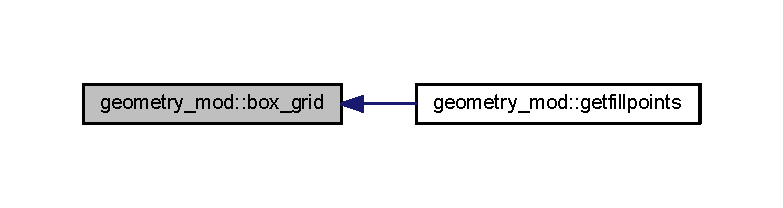
\includegraphics[width=336pt]{namespacegeometry__mod_ae87e4ecff2d21a839da2b82919b5fd0b_icgraph}
\end{center}
\end{figure}
\mbox{\Hypertarget{namespacegeometry__mod_a1d97564e04562532b5389bfb91aa676b}\label{namespacegeometry__mod_a1d97564e04562532b5389bfb91aa676b}} 
\index{geometry\+\_\+mod@{geometry\+\_\+mod}!fill@{fill}}
\index{fill@{fill}!geometry\+\_\+mod@{geometry\+\_\+mod}}
\subsubsection{\texorpdfstring{fill()}{fill()}}
{\footnotesize\ttfamily subroutine geometry\+\_\+mod\+::fill (\begin{DoxyParamCaption}\item[{class(\mbox{\hyperlink{structgeometry__mod_1_1geometry__class}{geometry\+\_\+class}}), intent(in)}]{self,  }\item[{class(\mbox{\hyperlink{structgeometry__mod_1_1shape}{shape}})}]{shapetype,  }\item[{real(prec), intent(in)}]{dp,  }\item[{integer, intent(in)}]{fillsize,  }\item[{type(vector), dimension(\mbox{\hyperlink{namespacegeometry__mod_ad790edd694561b33dad20cfa3a14e8f2}{fillsize}}), intent(out)}]{ptlist }\end{DoxyParamCaption})\hspace{0.3cm}{\ttfamily [private]}}



method to get the list of points that fill a given geometry 

\begin{DoxyAuthor}{Author}
Ricardo Birjukovs Canelas -\/ M\+A\+R\+E\+T\+EC 
\end{DoxyAuthor}

\begin{DoxyParams}[1]{Parameters}
\mbox{\tt in}  & {\em self,shapetype,dp,fillsize,ptlist} & \\
\hline
\end{DoxyParams}


Definition at line 147 of file geometry.\+f90.


\begin{DoxyCode}
147     \textcolor{keywordtype}{implicit none}
148     \textcolor{keywordtype}{class}(geometry\_class), \textcolor{keywordtype}{intent(in)} :: self
149     \textcolor{keywordtype}{class}(shape) :: shapetype
150     \textcolor{keywordtype}{real(prec)}, \textcolor{keywordtype}{intent(in)} :: dp
151     \textcolor{keywordtype}{integer}, \textcolor{keywordtype}{intent(in)} :: fillsize
152     \textcolor{keywordtype}{type}(vector), \textcolor{keywordtype}{intent(out)} :: ptlist(fillsize)
153     \textcolor{keywordtype}{type}(vector) :: temp
154     \textcolor{keywordtype}{type}(string) :: outext
155     \textcolor{keywordflow}{select type} (shapetype)
156 \textcolor{keywordflow}{    type is} (shape)
157 \textcolor{keywordflow}{    class is} (box)
158         \textcolor{keyword}{call }box\_grid(dp, shapetype%size, fillsize, ptlist)
159 \textcolor{keywordflow}{    class is} (point)
160         ptlist(1)=0
161 \textcolor{keywordflow}{    class is} (line)
162         \textcolor{keyword}{call }line\_grid(dp, geo2m(shapetype%last-shapetype%pt, shapetype%pt%y), fillsize, ptlist)
163 \textcolor{keywordflow}{    class is} (sphere)
164         \textcolor{keyword}{call }sphere\_grid(dp, shapetype%radius, fillsize, ptlist)
165 \textcolor{keywordflow}{        class default}
166         outext=\textcolor{stringliteral}{'[geometry::fill] : unexpected type for geometry object, stoping'}
167         \textcolor{keyword}{call }log%put(outext)
168         stop
169 \textcolor{keywordflow}{    end select}
\end{DoxyCode}
Here is the call graph for this function\+:\nopagebreak
\begin{figure}[H]
\begin{center}
\leavevmode
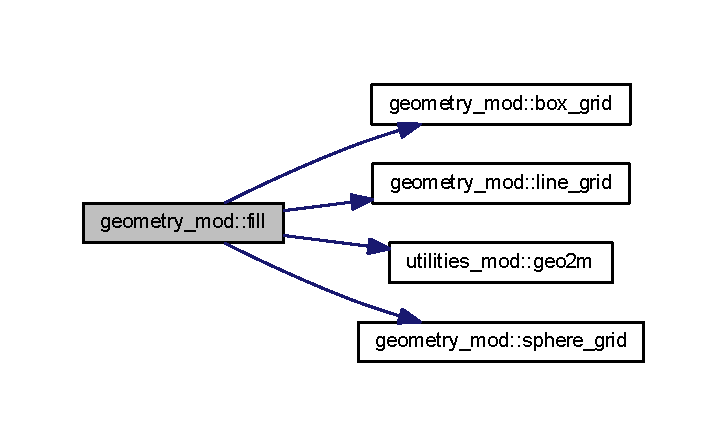
\includegraphics[width=349pt]{namespacegeometry__mod_a1d97564e04562532b5389bfb91aa676b_cgraph}
\end{center}
\end{figure}
\mbox{\Hypertarget{namespacegeometry__mod_ad790edd694561b33dad20cfa3a14e8f2}\label{namespacegeometry__mod_ad790edd694561b33dad20cfa3a14e8f2}} 
\index{geometry\+\_\+mod@{geometry\+\_\+mod}!fillsize@{fillsize}}
\index{fillsize@{fillsize}!geometry\+\_\+mod@{geometry\+\_\+mod}}
\subsubsection{\texorpdfstring{fillsize()}{fillsize()}}
{\footnotesize\ttfamily integer function geometry\+\_\+mod\+::fillsize (\begin{DoxyParamCaption}\item[{class(\mbox{\hyperlink{structgeometry__mod_1_1geometry__class}{geometry\+\_\+class}}), intent(in)}]{self,  }\item[{class(\mbox{\hyperlink{structgeometry__mod_1_1shape}{shape}}), intent(in)}]{shapetype,  }\item[{real(prec), intent(in)}]{dp }\end{DoxyParamCaption})\hspace{0.3cm}{\ttfamily [private]}}



method to get the number of points that fill a given geometry 

\begin{DoxyAuthor}{Author}
Ricardo Birjukovs Canelas -\/ M\+A\+R\+E\+T\+EC 
\end{DoxyAuthor}

\begin{DoxyParams}[1]{Parameters}
\mbox{\tt in}  & {\em self,shapetype,dp} & \\
\hline
\end{DoxyParams}


Definition at line 114 of file geometry.\+f90.


\begin{DoxyCode}
114     \textcolor{keywordtype}{implicit none}
115     \textcolor{keywordtype}{class}(geometry\_class), \textcolor{keywordtype}{intent(in)} :: self
116     \textcolor{keywordtype}{class}(shape), \textcolor{keywordtype}{intent(in)} :: shapetype
117     \textcolor{keywordtype}{real(prec)}, \textcolor{keywordtype}{intent(in)} :: dp
118     \textcolor{keywordtype}{integer} :: fillsize
119     \textcolor{keywordtype}{type}(vector) :: temp
120     \textcolor{keywordtype}{type}(string) :: outext
121     \textcolor{keywordflow}{select type} (shapetype)
122 \textcolor{keywordflow}{    type is} (shape)
123 \textcolor{keywordflow}{    class is} (box)
124         fillsize = max((int(shapetype%size%x/dp)+1)*(int(shapetype%size%y/dp)+1)*(int(shapetype%size%z/dp)+
      1),1)
125 \textcolor{keywordflow}{    class is} (point)
126         fillsize = 1
127 \textcolor{keywordflow}{    class is} (line)
128         temp = shapetype%pt - shapetype%last
129         temp = geo2m(temp, shapetype%pt%y)
130         fillsize = max(int(temp%normL2()/dp),1)
131 \textcolor{keywordflow}{    class is} (sphere)
132         fillsize = sphere\_np\_count(dp, shapetype%radius)
133 \textcolor{keywordflow}{        class default}
134         outext=\textcolor{stringliteral}{'[geometry::fillsize] : unexpected type for geometry object, stoping'}
135         \textcolor{keyword}{call }log%put(outext)
136         stop
137 \textcolor{keywordflow}{    end select}
\end{DoxyCode}
Here is the call graph for this function\+:\nopagebreak
\begin{figure}[H]
\begin{center}
\leavevmode
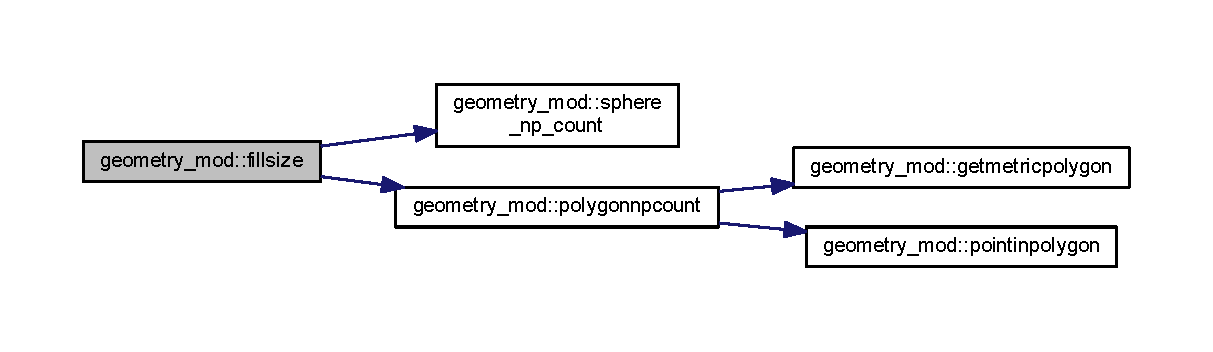
\includegraphics[width=346pt]{namespacegeometry__mod_ad790edd694561b33dad20cfa3a14e8f2_cgraph}
\end{center}
\end{figure}
\mbox{\Hypertarget{namespacegeometry__mod_a4a38edbff02aa0ff5f16a16c39bf778e}\label{namespacegeometry__mod_a4a38edbff02aa0ff5f16a16c39bf778e}} 
\index{geometry\+\_\+mod@{geometry\+\_\+mod}!getcenter@{getcenter}}
\index{getcenter@{getcenter}!geometry\+\_\+mod@{geometry\+\_\+mod}}
\subsubsection{\texorpdfstring{getcenter()}{getcenter()}}
{\footnotesize\ttfamily type(vector) function geometry\+\_\+mod\+::getcenter (\begin{DoxyParamCaption}\item[{class(\mbox{\hyperlink{structgeometry__mod_1_1geometry__class}{geometry\+\_\+class}}), intent(in)}]{self,  }\item[{class(\mbox{\hyperlink{structgeometry__mod_1_1shape}{shape}}), intent(in)}]{shapetype }\end{DoxyParamCaption})\hspace{0.3cm}{\ttfamily [private]}}



method to get the baricenter of a given geometry 

\begin{DoxyAuthor}{Author}
Ricardo Birjukovs Canelas -\/ M\+A\+R\+E\+T\+EC 
\end{DoxyAuthor}

\begin{DoxyParams}[1]{Parameters}
\mbox{\tt in}  & {\em self,shapetype} & \\
\hline
\end{DoxyParams}


Definition at line 179 of file geometry.\+f90.


\begin{DoxyCode}
179     \textcolor{keywordtype}{implicit none}
180     \textcolor{keywordtype}{class}(geometry\_class), \textcolor{keywordtype}{intent(in)} :: self
181     \textcolor{keywordtype}{class}(shape), \textcolor{keywordtype}{intent(in)} :: shapetype
182     \textcolor{keywordtype}{type}(vector) :: center
183     \textcolor{keywordtype}{type}(string) :: outext
184     \textcolor{keywordflow}{select type} (shapetype)
185 \textcolor{keywordflow}{    type is} (shape)
186 \textcolor{keywordflow}{    class is} (box)
187         center = shapetype%pt + m2geo(shapetype%size, shapetype%pt%y)/2.0
188 \textcolor{keywordflow}{    class is} (point)
189         center = shapetype%pt
190 \textcolor{keywordflow}{    class is} (line)
191         center = shapetype%pt + shapetype%last/2.0
192 \textcolor{keywordflow}{    class is} (sphere)
193         center = shapetype%pt
194 \textcolor{keywordflow}{        class default}
195         outext=\textcolor{stringliteral}{'[geometry::getCenter] : unexpected type for geometry object, stoping'}
196         \textcolor{keyword}{call }log%put(outext)
197         stop
198 \textcolor{keywordflow}{    end select}
\end{DoxyCode}
Here is the call graph for this function\+:\nopagebreak
\begin{figure}[H]
\begin{center}
\leavevmode
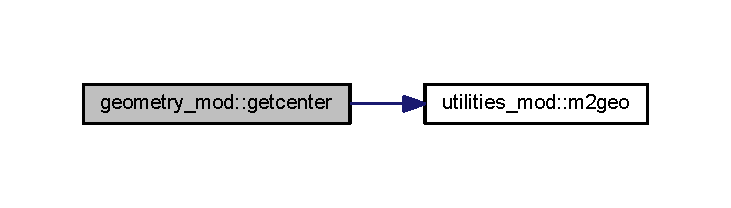
\includegraphics[width=350pt]{namespacegeometry__mod_a4a38edbff02aa0ff5f16a16c39bf778e_cgraph}
\end{center}
\end{figure}
\mbox{\Hypertarget{namespacegeometry__mod_a524c5d28a80fb6729b102126485605ce}\label{namespacegeometry__mod_a524c5d28a80fb6729b102126485605ce}} 
\index{geometry\+\_\+mod@{geometry\+\_\+mod}!getnumpoints@{getnumpoints}}
\index{getnumpoints@{getnumpoints}!geometry\+\_\+mod@{geometry\+\_\+mod}}
\subsubsection{\texorpdfstring{getnumpoints()}{getnumpoints()}}
{\footnotesize\ttfamily integer function geometry\+\_\+mod\+::getnumpoints (\begin{DoxyParamCaption}\item[{class(\mbox{\hyperlink{structgeometry__mod_1_1geometry__class}{geometry\+\_\+class}}), intent(in)}]{self,  }\item[{class(\mbox{\hyperlink{structgeometry__mod_1_1shape}{shape}}), intent(in)}]{shapetype }\end{DoxyParamCaption})\hspace{0.3cm}{\ttfamily [private]}}



method the points defining a given geometry 

\begin{DoxyAuthor}{Author}
Ricardo Birjukovs Canelas -\/ M\+A\+R\+E\+T\+EC 
\end{DoxyAuthor}

\begin{DoxyParams}[1]{Parameters}
\mbox{\tt in}  & {\em self,shapetype} & \\
\hline
\end{DoxyParams}


Definition at line 256 of file geometry.\+f90.


\begin{DoxyCode}
256     \textcolor{keywordtype}{class}(geometry\_class), \textcolor{keywordtype}{intent(in)} :: self
257     \textcolor{keywordtype}{class}(shape), \textcolor{keywordtype}{intent(in)} :: shapetype
258     \textcolor{keywordtype}{integer} :: n
259     \textcolor{keywordtype}{type}(string) :: outext
260     \textcolor{keywordflow}{select type} (shapetype)
261 \textcolor{keywordflow}{    type is} (shape)
262 \textcolor{keywordflow}{    class is} (box)
263         n=8
264 \textcolor{keywordflow}{    class is} (point)
265         n=1
266 \textcolor{keywordflow}{    class is} (line)
267         n=2
268 \textcolor{keywordflow}{    class is} (sphere)
269         n=1
270 \textcolor{keywordflow}{        class default}
271         outext=\textcolor{stringliteral}{'[geometry::getnumPoints] : unexpected type for geometry object, stoping'}
272         \textcolor{keyword}{call }log%put(outext)
273         stop
274 \textcolor{keywordflow}{    end select}
\end{DoxyCode}
\mbox{\Hypertarget{namespacegeometry__mod_a0b1a3c5aa414292ace34d59487082e3a}\label{namespacegeometry__mod_a0b1a3c5aa414292ace34d59487082e3a}} 
\index{geometry\+\_\+mod@{geometry\+\_\+mod}!getpoints@{getpoints}}
\index{getpoints@{getpoints}!geometry\+\_\+mod@{geometry\+\_\+mod}}
\subsubsection{\texorpdfstring{getpoints()}{getpoints()}}
{\footnotesize\ttfamily type(vector) function, dimension(\+:), allocatable geometry\+\_\+mod\+::getpoints (\begin{DoxyParamCaption}\item[{class(\mbox{\hyperlink{structgeometry__mod_1_1geometry__class}{geometry\+\_\+class}}), intent(in)}]{self,  }\item[{class(\mbox{\hyperlink{structgeometry__mod_1_1shape}{shape}}), intent(in)}]{shapetype }\end{DoxyParamCaption})\hspace{0.3cm}{\ttfamily [private]}}



method that returns the points defining a given geometry 

\begin{DoxyAuthor}{Author}
Ricardo Birjukovs Canelas -\/ M\+A\+R\+E\+T\+EC 
\end{DoxyAuthor}

\begin{DoxyParams}[1]{Parameters}
\mbox{\tt in}  & {\em self,shapetype} & \\
\hline
\end{DoxyParams}


Definition at line 208 of file geometry.\+f90.


\begin{DoxyCode}
208     \textcolor{keywordtype}{class}(geometry\_class), \textcolor{keywordtype}{intent(in)} :: self
209     \textcolor{keywordtype}{class}(shape), \textcolor{keywordtype}{intent(in)} :: shapetype
210     \textcolor{keywordtype}{type}(vector), \textcolor{keywordtype}{allocatable} :: pts(:)
211     \textcolor{keywordtype}{type}(string) :: outext
212     \textcolor{keywordtype}{integer} :: n
213     \textcolor{keywordtype}{type}(vector) :: temp
214     \textcolor{keywordflow}{select type} (shapetype)
215 \textcolor{keywordflow}{    type is} (shape)
216 \textcolor{keywordflow}{    class is} (box)
217         n=8
218         \textcolor{keyword}{allocate}(pts(n))
219         temp = shapetype%size
220         \textcolor{comment}{!temp = m2geo(shapetype%size, shapetype%pt%y)}
221         pts(1) = shapetype%pt
222         pts(2) = shapetype%pt + temp%y*ey
223         pts(3) = pts(2) + temp%z*ez
224         pts(4) = shapetype%pt + temp%z*ez
225         pts(5) = shapetype%pt + temp%x*ex
226         pts(6) = pts(5) + temp%y*ey
227         pts(7) = shapetype%pt + temp
228         pts(8) = pts(5) + temp%z*ez
229 \textcolor{keywordflow}{    class is} (point)
230         n=1
231         \textcolor{keyword}{allocate}(pts(n))
232         pts(1) = shapetype%pt
233 \textcolor{keywordflow}{    class is} (line)
234         n=2
235         \textcolor{keyword}{allocate}(pts(n))
236         pts(1) = shapetype%pt
237         pts(2) = shapetype%last
238 \textcolor{keywordflow}{    class is} (sphere)
239         n=1
240         \textcolor{keyword}{allocate}(pts(n))
241         pts(1) = shapetype%pt
242 \textcolor{keywordflow}{        class default}
243         outext=\textcolor{stringliteral}{'[geometry::getPoints] : unexpected type for geometry object, stoping'}
244         \textcolor{keyword}{call }log%put(outext)
245         stop
246 \textcolor{keywordflow}{    end select}
\end{DoxyCode}
\mbox{\Hypertarget{namespacegeometry__mod_a22dd77024fce56da299445a697256155}\label{namespacegeometry__mod_a22dd77024fce56da299445a697256155}} 
\index{geometry\+\_\+mod@{geometry\+\_\+mod}!inlist@{inlist}}
\index{inlist@{inlist}!geometry\+\_\+mod@{geometry\+\_\+mod}}
\subsubsection{\texorpdfstring{inlist()}{inlist()}}
{\footnotesize\ttfamily logical function geometry\+\_\+mod\+::inlist (\begin{DoxyParamCaption}\item[{class(\mbox{\hyperlink{structgeometry__mod_1_1geometry__class}{geometry\+\_\+class}}), intent(in)}]{self,  }\item[{type(string), intent(in)}]{geomname }\end{DoxyParamCaption})\hspace{0.3cm}{\ttfamily [private]}}



Public function that returns a logical if the input geometry name is valid. 

\begin{DoxyAuthor}{Author}
Ricardo Birjukovs Canelas -\/ M\+A\+R\+E\+T\+EC 
\end{DoxyAuthor}

\begin{DoxyParams}[1]{Parameters}
\mbox{\tt in}  & {\em self,geomname} & \\
\hline
\end{DoxyParams}


Definition at line 95 of file geometry.\+f90.


\begin{DoxyCode}
95     \textcolor{keywordtype}{implicit none}
96     \textcolor{keywordtype}{class}(geometry\_class), \textcolor{keywordtype}{intent(in)} :: self
97     \textcolor{keywordtype}{type}(string), \textcolor{keywordtype}{intent(in)} :: geomname
98     \textcolor{keywordtype}{integer} :: i
99     tf = .false.
100     \textcolor{keywordflow}{do} i=1, \textcolor{keyword}{size}(self%list)
101         \textcolor{keywordflow}{if} (geomname == self%list(i)) \textcolor{keywordflow}{then}
102             tf = .true.
103 \textcolor{keywordflow}{        endif}
104 \textcolor{keywordflow}{    enddo}
\end{DoxyCode}
\mbox{\Hypertarget{namespacegeometry__mod_abcb09c0f5274c27cb79b0dd009ed94b3}\label{namespacegeometry__mod_abcb09c0f5274c27cb79b0dd009ed94b3}} 
\index{geometry\+\_\+mod@{geometry\+\_\+mod}!line\+\_\+grid@{line\+\_\+grid}}
\index{line\+\_\+grid@{line\+\_\+grid}!geometry\+\_\+mod@{geometry\+\_\+mod}}
\subsubsection{\texorpdfstring{line\+\_\+grid()}{line\_grid()}}
{\footnotesize\ttfamily subroutine geometry\+\_\+mod\+::line\+\_\+grid (\begin{DoxyParamCaption}\item[{real(prec), intent(in)}]{dp,  }\item[{type(vector), intent(in)}]{dist,  }\item[{integer, intent(in)}]{np,  }\item[{type(vector), dimension(np), intent(out)}]{ptlist }\end{DoxyParamCaption})\hspace{0.3cm}{\ttfamily [private]}}



private routine that returns the points distributed on a grid with spacing dp along a line 

\begin{DoxyAuthor}{Author}
Ricardo Birjukovs Canelas -\/ M\+A\+R\+E\+T\+EC 
\end{DoxyAuthor}

\begin{DoxyParams}[1]{Parameters}
\mbox{\tt in}  & {\em dp,dist,np,ptlist} & \\
\hline
\end{DoxyParams}


Definition at line 425 of file geometry.\+f90.


\begin{DoxyCode}
425     \textcolor{keywordtype}{implicit none}
426     \textcolor{keywordtype}{real(prec)}, \textcolor{keywordtype}{intent(in)} :: dp
427     \textcolor{keywordtype}{type}(vector), \textcolor{keywordtype}{intent(in)} :: dist
428     \textcolor{keywordtype}{integer}, \textcolor{keywordtype}{intent(in)}::  np
429     \textcolor{keywordtype}{type}(vector), \textcolor{keywordtype}{intent(out)} :: ptlist(np)
430     \textcolor{keywordtype}{integer} :: i, j, k, p
431 
432     \textcolor{keywordflow}{do} p=1, np
433         ptlist(p) = dp/np*(dist*(p-1))
434 \textcolor{keywordflow}{    end do}
435     \textcolor{keywordflow}{if} (np == 1) \textcolor{keywordflow}{then} \textcolor{comment}{!Just the origin}
436         ptlist(1)= 0*ex + 0*ey +0*ez
437 \textcolor{keywordflow}{    end if}
\end{DoxyCode}
Here is the caller graph for this function\+:\nopagebreak
\begin{figure}[H]
\begin{center}
\leavevmode
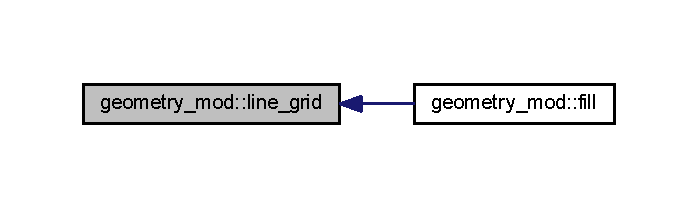
\includegraphics[width=335pt]{namespacegeometry__mod_abcb09c0f5274c27cb79b0dd009ed94b3_icgraph}
\end{center}
\end{figure}
\mbox{\Hypertarget{namespacegeometry__mod_aed4426181ca851b41717edd50268e5f3}\label{namespacegeometry__mod_aed4426181ca851b41717edd50268e5f3}} 
\index{geometry\+\_\+mod@{geometry\+\_\+mod}!printgeometry@{printgeometry}}
\index{printgeometry@{printgeometry}!geometry\+\_\+mod@{geometry\+\_\+mod}}
\subsubsection{\texorpdfstring{printgeometry()}{printgeometry()}}
{\footnotesize\ttfamily subroutine geometry\+\_\+mod\+::printgeometry (\begin{DoxyParamCaption}\item[{class(\mbox{\hyperlink{structgeometry__mod_1_1geometry__class}{geometry\+\_\+class}}), intent(in)}]{self,  }\item[{class(\mbox{\hyperlink{structgeometry__mod_1_1shape}{shape}})}]{shapetype }\end{DoxyParamCaption})\hspace{0.3cm}{\ttfamily [private]}}



method to print the details of a given geometry 

\begin{DoxyAuthor}{Author}
Ricardo Birjukovs Canelas -\/ M\+A\+R\+E\+T\+EC 
\end{DoxyAuthor}

\begin{DoxyParams}[1]{Parameters}
\mbox{\tt in}  & {\em self,shapetype} & \\
\hline
\end{DoxyParams}


Definition at line 284 of file geometry.\+f90.


\begin{DoxyCode}
284     \textcolor{keywordtype}{implicit none}
285     \textcolor{keywordtype}{class}(geometry\_class), \textcolor{keywordtype}{intent(in)} :: self
286     \textcolor{keywordtype}{class}(shape) :: shapetype
287 
288     \textcolor{keywordtype}{type}(vector) :: temp(2)
289     \textcolor{keywordtype}{type}(string) :: temp\_str(6)
290     \textcolor{keywordtype}{type}(string) :: outext
291 
292     temp\_str(1) = shapetype%pt%x
293     temp\_str(2) = shapetype%pt%y
294     temp\_str(3) = shapetype%pt%z
295     \textcolor{keywordflow}{select type} (shapetype)
296 \textcolor{keywordflow}{    type is} (shape)
297 \textcolor{keywordflow}{    class is} (box)
298         temp\_str(4) = shapetype%size%x
299         temp\_str(5) = shapetype%size%y
300         temp\_str(6) = shapetype%size%z
301         outext=\textcolor{stringliteral}{'      Box at '}//temp\_str(1)//\textcolor{stringliteral}{' '}//temp\_str(2)//\textcolor{stringliteral}{' '}//temp\_str(3)//new\_line(\textcolor{stringliteral}{'a'})//&
302             \textcolor{stringliteral}{'       with '}//temp\_str(4)//\textcolor{stringliteral}{' X '}//temp\_str(5)//\textcolor{stringliteral}{' X '}//temp\_str(6)
303 \textcolor{keywordflow}{    class is} (point)
304         outext=\textcolor{stringliteral}{'      Point at '}//temp\_str(1)//\textcolor{stringliteral}{' '}//temp\_str(2)//\textcolor{stringliteral}{' '}//temp\_str(3)
305 \textcolor{keywordflow}{    class is} (line)
306         temp\_str(4) = shapetype%last%x
307         temp\_str(5) = shapetype%last%y
308         temp\_str(6) = shapetype%last%z
309         outext=\textcolor{stringliteral}{'      Line from '}//temp\_str(1)//\textcolor{stringliteral}{' '}//temp\_str(2)//\textcolor{stringliteral}{' '}//temp\_str(3)//new\_line(\textcolor{stringliteral}{'a'})//&
310             \textcolor{stringliteral}{'       to '}//temp\_str(4)//\textcolor{stringliteral}{' X '}//temp\_str(5)//\textcolor{stringliteral}{' X '}//temp\_str(6)
311 \textcolor{keywordflow}{    class is} (sphere)
312         temp\_str(4) = shapetype%radius
313         outext=\textcolor{stringliteral}{'      Sphere at '}//temp\_str(1)//\textcolor{stringliteral}{' '}//temp\_str(2)//\textcolor{stringliteral}{' '}//temp\_str(3)//new\_line(\textcolor{stringliteral}{'a'})//&
314             \textcolor{stringliteral}{'       with radius '}//temp\_str(4)
315 \textcolor{keywordflow}{        class default}
316         outext=\textcolor{stringliteral}{'[geometry::print] : unexpected type for geometry object, stoping'}
317         \textcolor{keyword}{call }log%put(outext)
318         stop
319 \textcolor{keywordflow}{    end select}
320     \textcolor{keyword}{call }log%put(outext,.false.)
321 
\end{DoxyCode}
\mbox{\Hypertarget{namespacegeometry__mod_a6c03a4ea3de6763940396dbeb3908ebc}\label{namespacegeometry__mod_a6c03a4ea3de6763940396dbeb3908ebc}} 
\index{geometry\+\_\+mod@{geometry\+\_\+mod}!sphere\+\_\+grid@{sphere\+\_\+grid}}
\index{sphere\+\_\+grid@{sphere\+\_\+grid}!geometry\+\_\+mod@{geometry\+\_\+mod}}
\subsubsection{\texorpdfstring{sphere\+\_\+grid()}{sphere\_grid()}}
{\footnotesize\ttfamily subroutine geometry\+\_\+mod\+::sphere\+\_\+grid (\begin{DoxyParamCaption}\item[{real(prec), intent(in)}]{dp,  }\item[{real(prec), intent(in)}]{r,  }\item[{integer, intent(in)}]{np,  }\item[{type(vector), dimension(np), intent(out)}]{ptlist }\end{DoxyParamCaption})\hspace{0.3cm}{\ttfamily [private]}}



private routine that returns the points distributed on a grid with spacing dp inside a sphere 

\begin{DoxyAuthor}{Author}
Ricardo Birjukovs Canelas -\/ M\+A\+R\+E\+T\+EC 
\end{DoxyAuthor}

\begin{DoxyParams}[1]{Parameters}
\mbox{\tt in}  & {\em dp,r,np,ptlist} & \\
\hline
\end{DoxyParams}


Definition at line 363 of file geometry.\+f90.


\begin{DoxyCode}
363     \textcolor{keywordtype}{implicit none}
364     \textcolor{keywordtype}{real(prec)}, \textcolor{keywordtype}{intent(in)} :: dp
365     \textcolor{keywordtype}{real(prec)}, \textcolor{keywordtype}{intent(in)} :: r
366     \textcolor{keywordtype}{integer}, \textcolor{keywordtype}{intent(in)}::  np
367     \textcolor{keywordtype}{type}(vector), \textcolor{keywordtype}{intent(out)} :: ptlist(np)
368     \textcolor{keywordtype}{integer} :: i, j, k, p, n
369     \textcolor{keywordtype}{type}(vector) :: pts
370     n=int(3*r/dp)
371     p=0
372     \textcolor{keywordflow}{do} i=1, n
373         \textcolor{keywordflow}{do} j=1, n
374             \textcolor{keywordflow}{do} k=1, n
375                 pts = dp*(ex*(i-1)+ey*(j-1)+ez*(k-1)) - r*(ex+ey+ez)
376                 \textcolor{keywordflow}{if} (pts%normL2() .le. r) \textcolor{keywordflow}{then}
377                     p=p+1
378                     ptlist(p)=pts
379 \textcolor{keywordflow}{                end if}
380 \textcolor{keywordflow}{            end do}
381 \textcolor{keywordflow}{        end do}
382 \textcolor{keywordflow}{    end do}
383     \textcolor{keywordflow}{if} (np == 1) \textcolor{keywordflow}{then} \textcolor{comment}{!Just the center point}
384         ptlist(1)= 0*ex + 0*ey +0*ez
385 \textcolor{keywordflow}{    end if}
386 
\end{DoxyCode}
Here is the caller graph for this function\+:\nopagebreak
\begin{figure}[H]
\begin{center}
\leavevmode
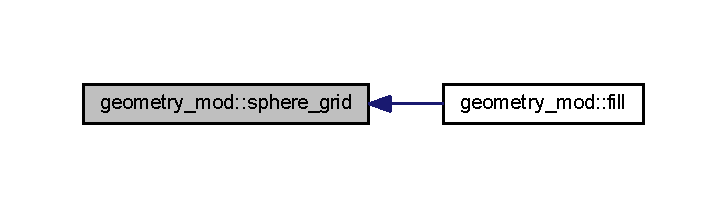
\includegraphics[width=349pt]{namespacegeometry__mod_a6c03a4ea3de6763940396dbeb3908ebc_icgraph}
\end{center}
\end{figure}
\mbox{\Hypertarget{namespacegeometry__mod_a05de7940b4e7df5a2b31f3d0414e3743}\label{namespacegeometry__mod_a05de7940b4e7df5a2b31f3d0414e3743}} 
\index{geometry\+\_\+mod@{geometry\+\_\+mod}!sphere\+\_\+np\+\_\+count@{sphere\+\_\+np\+\_\+count}}
\index{sphere\+\_\+np\+\_\+count@{sphere\+\_\+np\+\_\+count}!geometry\+\_\+mod@{geometry\+\_\+mod}}
\subsubsection{\texorpdfstring{sphere\+\_\+np\+\_\+count()}{sphere\_np\_count()}}
{\footnotesize\ttfamily integer function geometry\+\_\+mod\+::sphere\+\_\+np\+\_\+count (\begin{DoxyParamCaption}\item[{real(prec), intent(in)}]{dp,  }\item[{real(prec), intent(in)}]{r }\end{DoxyParamCaption})\hspace{0.3cm}{\ttfamily [private]}}



private function that returns the number of points distributed on a grid with spacing dp inside a sphere 

\begin{DoxyAuthor}{Author}
Ricardo Birjukovs Canelas -\/ M\+A\+R\+E\+T\+EC 
\end{DoxyAuthor}

\begin{DoxyParams}[1]{Parameters}
\mbox{\tt in}  & {\em dp,r} & \\
\hline
\end{DoxyParams}


Definition at line 332 of file geometry.\+f90.


\begin{DoxyCode}
332     \textcolor{keywordtype}{implicit none}
333     \textcolor{keywordtype}{real(prec)}, \textcolor{keywordtype}{intent(in)} :: dp
334     \textcolor{keywordtype}{real(prec)}, \textcolor{keywordtype}{intent(in)} :: r
335     \textcolor{keywordtype}{integer} :: np
336     \textcolor{keywordtype}{integer} :: i, j, k, n
337     \textcolor{keywordtype}{type}(vector) :: pts
338     np=0
339     n=int(3*r/dp)
340     \textcolor{keywordflow}{do} i=1, n
341         \textcolor{keywordflow}{do} j=1, n
342             \textcolor{keywordflow}{do} k=1, n
343                 pts = dp*(ex*(i-1)+ey*(j-1)+ez*(k-1)) - r*(ex+ey+ez)
344                 \textcolor{keywordflow}{if} (pts%normL2() .le. r) \textcolor{keywordflow}{then}
345                     np=np+1
346 \textcolor{keywordflow}{                end if}
347 \textcolor{keywordflow}{            end do}
348 \textcolor{keywordflow}{        end do}
349 \textcolor{keywordflow}{    end do}
350     \textcolor{keywordflow}{if} (np == 0) \textcolor{keywordflow}{then} \textcolor{comment}{!Just the center point}
351         np=1
352 \textcolor{keywordflow}{    end if}
\end{DoxyCode}
Here is the caller graph for this function\+:\nopagebreak
\begin{figure}[H]
\begin{center}
\leavevmode
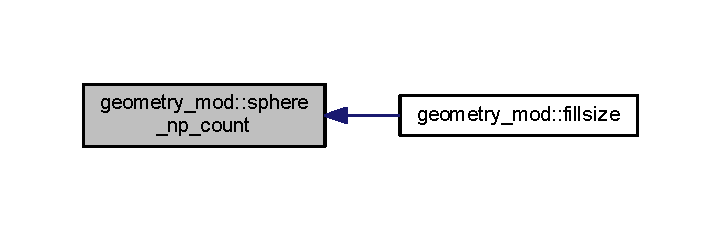
\includegraphics[width=346pt]{namespacegeometry__mod_a05de7940b4e7df5a2b31f3d0414e3743_icgraph}
\end{center}
\end{figure}


\subsection{Variable Documentation}
\mbox{\Hypertarget{namespacegeometry__mod_ad2ad4f7e1138beaad5f37d5c15b7b457}\label{namespacegeometry__mod_ad2ad4f7e1138beaad5f37d5c15b7b457}} 
\index{geometry\+\_\+mod@{geometry\+\_\+mod}!geometry@{geometry}}
\index{geometry@{geometry}!geometry\+\_\+mod@{geometry\+\_\+mod}}
\subsubsection{\texorpdfstring{geometry}{geometry}}
{\footnotesize\ttfamily type(\mbox{\hyperlink{structgeometry__mod_1_1geometry__class}{geometry\+\_\+class}}), public geometry\+\_\+mod\+::geometry}



Definition at line 65 of file geometry.\+f90.


\begin{DoxyCode}
65     \textcolor{keywordtype}{type}(geometry\_class) :: Geometry
\end{DoxyCode}

\hypertarget{namespacelink__mod}{}\section{link\+\_\+mod Module Reference}
\label{namespacelink__mod}\index{link\+\_\+mod@{link\+\_\+mod}}


Module that defines a link based on an unlimited polymorphic container class.  


\subsection*{Data Types}
\begin{DoxyCompactItemize}
\item 
interface \mbox{\hyperlink{structlink__mod_1_1link}{link}}
\end{DoxyCompactItemize}
\subsection*{Functions/\+Subroutines}
\begin{DoxyCompactItemize}
\item 
class($\ast$) function, pointer \mbox{\hyperlink{namespacelink__mod_aa2c8d19ee91797e19464fc7589cc2c39}{getvalue}} (this)
\begin{DoxyCompactList}\small\item\em Method that returns a pointer to the values stored in the container in this link. \end{DoxyCompactList}\item 
class(\mbox{\hyperlink{structlink__mod_1_1link}{link}}) function, pointer \mbox{\hyperlink{namespacelink__mod_a2d776121ed0138aba8b3d166938c964f}{nextlink}} (this)
\begin{DoxyCompactList}\small\item\em Method that returns a pointer to the next link in a list. \end{DoxyCompactList}\item 
class(\mbox{\hyperlink{structlink__mod_1_1link}{link}}) function, pointer \mbox{\hyperlink{namespacelink__mod_a2d23022ef22049f8340099b6960d8d5d}{previouslink}} (this)
\begin{DoxyCompactList}\small\item\em Method that returns a pointer to the previous link in a list. \end{DoxyCompactList}\item 
subroutine \mbox{\hyperlink{namespacelink__mod_a0dd2fe581e8d566faf03fc7ebd2f8524}{setnextlink}} (this, next)
\begin{DoxyCompactList}\small\item\em Method to set the next link in a list. \end{DoxyCompactList}\item 
subroutine \mbox{\hyperlink{namespacelink__mod_ad0d413cb7907fdcf6561639cdd03481a}{setpreviouslink}} (this, prev)
\begin{DoxyCompactList}\small\item\em Method to set the previous link in a list. \end{DoxyCompactList}\item 
subroutine \mbox{\hyperlink{namespacelink__mod_ae2d89f23eb8cf4b8065b8a39e9902a22}{removelink}} (this)
\begin{DoxyCompactList}\small\item\em Method to remove a link in a list. \end{DoxyCompactList}\item 
class(\mbox{\hyperlink{structlink__mod_1_1link}{link}}) function, pointer \mbox{\hyperlink{namespacelink__mod_ac5b4f1702d8edb10a4559f6f371dc797}{constructor}} (to\+\_\+store, prev, next, key)
\begin{DoxyCompactList}\small\item\em Link constructor, can be used with the \textquotesingle{}link\textquotesingle{} name since it was defined as such in an interface declaration. \end{DoxyCompactList}\end{DoxyCompactItemize}


\subsection{Detailed Description}
Module that defines a link based on an unlimited polymorphic container class. 

\begin{DoxyAuthor}{Author}
Ricardo Birjukovs Canelas 
\end{DoxyAuthor}


\subsection{Function/\+Subroutine Documentation}
\mbox{\Hypertarget{namespacelink__mod_ac5b4f1702d8edb10a4559f6f371dc797}\label{namespacelink__mod_ac5b4f1702d8edb10a4559f6f371dc797}} 
\index{link\+\_\+mod@{link\+\_\+mod}!constructor@{constructor}}
\index{constructor@{constructor}!link\+\_\+mod@{link\+\_\+mod}}
\subsubsection{\texorpdfstring{constructor()}{constructor()}}
{\footnotesize\ttfamily class(\mbox{\hyperlink{structlink__mod_1_1link}{link}}) function, pointer link\+\_\+mod\+::constructor (\begin{DoxyParamCaption}\item[{class($\ast$), intent(in)}]{to\+\_\+store,  }\item[{class(\mbox{\hyperlink{structlink__mod_1_1link}{link}}), intent(in), pointer}]{prev,  }\item[{class(\mbox{\hyperlink{structlink__mod_1_1link}{link}}), intent(in), pointer}]{next,  }\item[{integer, intent(in), optional}]{key }\end{DoxyParamCaption})\hspace{0.3cm}{\ttfamily [private]}}



Link constructor, can be used with the \textquotesingle{}link\textquotesingle{} name since it was defined as such in an interface declaration. 

\begin{DoxyAuthor}{Author}
Ricardo Birjukovs Canelas -\/ M\+A\+R\+E\+T\+EC 
\end{DoxyAuthor}

\begin{DoxyParams}[1]{Parameters}
\mbox{\tt in}  & {\em to\+\_\+store,prev,next,key} & \\
\hline
\end{DoxyParams}


Definition at line 134 of file link.\+f90.


\begin{DoxyCode}
134     \textcolor{keywordtype}{class}(link), \textcolor{keywordtype}{pointer} :: constructor
135     \textcolor{keywordtype}{class}(*), \textcolor{keywordtype}{intent(in)} :: to\_store
136     \textcolor{keywordtype}{class}(link), \textcolor{keywordtype}{pointer}, \textcolor{keywordtype}{intent(in)} :: prev
137     \textcolor{keywordtype}{class}(link), \textcolor{keywordtype}{pointer}, \textcolor{keywordtype}{intent(in)} :: next
138     \textcolor{keywordtype}{integer}, \textcolor{keywordtype}{intent(in)}, \textcolor{keywordtype}{optional} :: key
139     \textcolor{keyword}{allocate}(constructor)
140     \textcolor{keyword}{call }constructor%setPreviousLink(prev)
141     \textcolor{keyword}{call }constructor%setNextLink(next)
142     \textcolor{keyword}{call }constructor%storeContent(to\_store)
143     \textcolor{keywordflow}{if} (\textcolor{keyword}{present}(key)) \textcolor{keywordflow}{then}
144         constructor%key = key
145 \textcolor{keywordflow}{    end if}
\end{DoxyCode}
Here is the call graph for this function\+:\nopagebreak
\begin{figure}[H]
\begin{center}
\leavevmode
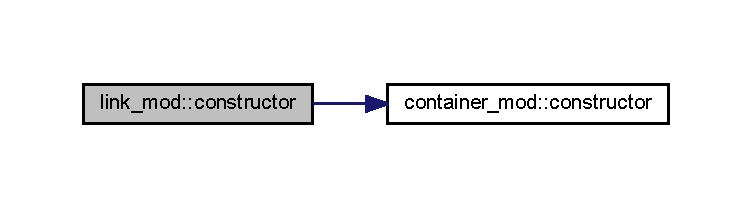
\includegraphics[width=350pt]{namespacelink__mod_ac5b4f1702d8edb10a4559f6f371dc797_cgraph}
\end{center}
\end{figure}
\mbox{\Hypertarget{namespacelink__mod_aa2c8d19ee91797e19464fc7589cc2c39}\label{namespacelink__mod_aa2c8d19ee91797e19464fc7589cc2c39}} 
\index{link\+\_\+mod@{link\+\_\+mod}!getvalue@{getvalue}}
\index{getvalue@{getvalue}!link\+\_\+mod@{link\+\_\+mod}}
\subsubsection{\texorpdfstring{getvalue()}{getvalue()}}
{\footnotesize\ttfamily class($\ast$) function, pointer link\+\_\+mod\+::getvalue (\begin{DoxyParamCaption}\item[{class(\mbox{\hyperlink{structlink__mod_1_1link}{link}})}]{this }\end{DoxyParamCaption})\hspace{0.3cm}{\ttfamily [private]}}



Method that returns a pointer to the values stored in the container in this link. 

\begin{DoxyAuthor}{Author}
Ricardo Birjukovs Canelas -\/ M\+A\+R\+E\+T\+EC 
\end{DoxyAuthor}


Definition at line 67 of file link.\+f90.


\begin{DoxyCode}
67     \textcolor{keywordtype}{class}(link) :: this
68     \textcolor{keywordtype}{class}(*), \textcolor{keywordtype}{pointer} :: getValue
69     getvalue => this%getContent()
\end{DoxyCode}
\mbox{\Hypertarget{namespacelink__mod_a2d776121ed0138aba8b3d166938c964f}\label{namespacelink__mod_a2d776121ed0138aba8b3d166938c964f}} 
\index{link\+\_\+mod@{link\+\_\+mod}!nextlink@{nextlink}}
\index{nextlink@{nextlink}!link\+\_\+mod@{link\+\_\+mod}}
\subsubsection{\texorpdfstring{nextlink()}{nextlink()}}
{\footnotesize\ttfamily class(\mbox{\hyperlink{structlink__mod_1_1link}{link}}) function, pointer link\+\_\+mod\+::nextlink (\begin{DoxyParamCaption}\item[{class(\mbox{\hyperlink{structlink__mod_1_1link}{link}})}]{this }\end{DoxyParamCaption})\hspace{0.3cm}{\ttfamily [private]}}



Method that returns a pointer to the next link in a list. 

\begin{DoxyAuthor}{Author}
Ricardo Birjukovs Canelas -\/ M\+A\+R\+E\+T\+EC 
\end{DoxyAuthor}


Definition at line 78 of file link.\+f90.


\begin{DoxyCode}
78     \textcolor{keywordtype}{class}(link) :: this
79     \textcolor{keywordtype}{class}(link), \textcolor{keywordtype}{pointer} :: nextLink
80     nextlink => this%next
\end{DoxyCode}
\mbox{\Hypertarget{namespacelink__mod_a2d23022ef22049f8340099b6960d8d5d}\label{namespacelink__mod_a2d23022ef22049f8340099b6960d8d5d}} 
\index{link\+\_\+mod@{link\+\_\+mod}!previouslink@{previouslink}}
\index{previouslink@{previouslink}!link\+\_\+mod@{link\+\_\+mod}}
\subsubsection{\texorpdfstring{previouslink()}{previouslink()}}
{\footnotesize\ttfamily class(\mbox{\hyperlink{structlink__mod_1_1link}{link}}) function, pointer link\+\_\+mod\+::previouslink (\begin{DoxyParamCaption}\item[{class(\mbox{\hyperlink{structlink__mod_1_1link}{link}})}]{this }\end{DoxyParamCaption})\hspace{0.3cm}{\ttfamily [private]}}



Method that returns a pointer to the previous link in a list. 

\begin{DoxyAuthor}{Author}
Ricardo Birjukovs Canelas -\/ M\+A\+R\+E\+T\+EC 
\end{DoxyAuthor}


Definition at line 89 of file link.\+f90.


\begin{DoxyCode}
89     \textcolor{keywordtype}{class}(link) :: this
90     \textcolor{keywordtype}{class}(link), \textcolor{keywordtype}{pointer} :: previousLink
91     previouslink => this%previous
\end{DoxyCode}
\mbox{\Hypertarget{namespacelink__mod_ae2d89f23eb8cf4b8065b8a39e9902a22}\label{namespacelink__mod_ae2d89f23eb8cf4b8065b8a39e9902a22}} 
\index{link\+\_\+mod@{link\+\_\+mod}!removelink@{removelink}}
\index{removelink@{removelink}!link\+\_\+mod@{link\+\_\+mod}}
\subsubsection{\texorpdfstring{removelink()}{removelink()}}
{\footnotesize\ttfamily subroutine link\+\_\+mod\+::removelink (\begin{DoxyParamCaption}\item[{class(\mbox{\hyperlink{structlink__mod_1_1link}{link}}), intent(inout)}]{this }\end{DoxyParamCaption})\hspace{0.3cm}{\ttfamily [private]}}



Method to remove a link in a list. 

\begin{DoxyAuthor}{Author}
Ricardo Birjukovs Canelas -\/ M\+A\+R\+E\+T\+EC 
\end{DoxyAuthor}


Definition at line 122 of file link.\+f90.


\begin{DoxyCode}
122     \textcolor{keywordtype}{class}(link), \textcolor{keywordtype}{intent(inout)} :: this
123     \textcolor{keyword}{call }this%deleteContent()
\end{DoxyCode}
\mbox{\Hypertarget{namespacelink__mod_a0dd2fe581e8d566faf03fc7ebd2f8524}\label{namespacelink__mod_a0dd2fe581e8d566faf03fc7ebd2f8524}} 
\index{link\+\_\+mod@{link\+\_\+mod}!setnextlink@{setnextlink}}
\index{setnextlink@{setnextlink}!link\+\_\+mod@{link\+\_\+mod}}
\subsubsection{\texorpdfstring{setnextlink()}{setnextlink()}}
{\footnotesize\ttfamily subroutine link\+\_\+mod\+::setnextlink (\begin{DoxyParamCaption}\item[{class(\mbox{\hyperlink{structlink__mod_1_1link}{link}})}]{this,  }\item[{class(\mbox{\hyperlink{structlink__mod_1_1link}{link}}), pointer}]{next }\end{DoxyParamCaption})\hspace{0.3cm}{\ttfamily [private]}}



Method to set the next link in a list. 

\begin{DoxyAuthor}{Author}
Ricardo Birjukovs Canelas -\/ M\+A\+R\+E\+T\+EC 
\end{DoxyAuthor}


Definition at line 100 of file link.\+f90.


\begin{DoxyCode}
100     \textcolor{keywordtype}{class}(link) :: this
101     \textcolor{keywordtype}{class}(link), \textcolor{keywordtype}{pointer} :: next
102     this%next => next
\end{DoxyCode}
\mbox{\Hypertarget{namespacelink__mod_ad0d413cb7907fdcf6561639cdd03481a}\label{namespacelink__mod_ad0d413cb7907fdcf6561639cdd03481a}} 
\index{link\+\_\+mod@{link\+\_\+mod}!setpreviouslink@{setpreviouslink}}
\index{setpreviouslink@{setpreviouslink}!link\+\_\+mod@{link\+\_\+mod}}
\subsubsection{\texorpdfstring{setpreviouslink()}{setpreviouslink()}}
{\footnotesize\ttfamily subroutine link\+\_\+mod\+::setpreviouslink (\begin{DoxyParamCaption}\item[{class(\mbox{\hyperlink{structlink__mod_1_1link}{link}})}]{this,  }\item[{class(\mbox{\hyperlink{structlink__mod_1_1link}{link}}), pointer}]{prev }\end{DoxyParamCaption})\hspace{0.3cm}{\ttfamily [private]}}



Method to set the previous link in a list. 

\begin{DoxyAuthor}{Author}
Ricardo Birjukovs Canelas -\/ M\+A\+R\+E\+T\+EC 
\end{DoxyAuthor}


Definition at line 111 of file link.\+f90.


\begin{DoxyCode}
111     \textcolor{keywordtype}{class}(link) :: this
112     \textcolor{keywordtype}{class}(link), \textcolor{keywordtype}{pointer} :: prev
113     this%previous => prev
\end{DoxyCode}

\hypertarget{namespacesimulation__about__mod}{}\section{simulation\+\_\+about\+\_\+mod Module Reference}
\label{namespacesimulation__about__mod}\index{simulation\+\_\+about\+\_\+mod@{simulation\+\_\+about\+\_\+mod}}


Module to print version, licence, preambles.  


\subsection*{Functions/\+Subroutines}
\begin{DoxyCompactItemize}
\item 
subroutine, public \mbox{\hyperlink{namespacesimulation__about__mod_ac436e98649d7488280cd176bbe765931}{printlicpreamble}}
\begin{DoxyCompactList}\small\item\em Public licence and preamble printer routine. \end{DoxyCompactList}\end{DoxyCompactItemize}
\subsection*{Variables}
\begin{DoxyCompactItemize}
\item 
type(string) \mbox{\hyperlink{namespacesimulation__about__mod_aa52b892695e36d427843d6e035b37d36}{version}}
\item 
type(string) \mbox{\hyperlink{namespacesimulation__about__mod_a49c4e8683dee7c3a2cd52658879c6e38}{author}}
\item 
type(string) \mbox{\hyperlink{namespacesimulation__about__mod_ad2ae0e434e2c6b0221094f181a538dc6}{date}}
\end{DoxyCompactItemize}


\subsection{Detailed Description}
Module to print version, licence, preambles. 

\begin{DoxyAuthor}{Author}
Ricardo Birjukovs Canelas 
\end{DoxyAuthor}


\subsection{Function/\+Subroutine Documentation}
\mbox{\Hypertarget{namespacesimulation__about__mod_ac436e98649d7488280cd176bbe765931}\label{namespacesimulation__about__mod_ac436e98649d7488280cd176bbe765931}} 
\index{simulation\+\_\+about\+\_\+mod@{simulation\+\_\+about\+\_\+mod}!printlicpreamble@{printlicpreamble}}
\index{printlicpreamble@{printlicpreamble}!simulation\+\_\+about\+\_\+mod@{simulation\+\_\+about\+\_\+mod}}
\subsubsection{\texorpdfstring{printlicpreamble()}{printlicpreamble()}}
{\footnotesize\ttfamily subroutine, public simulation\+\_\+about\+\_\+mod\+::printlicpreamble (\begin{DoxyParamCaption}{ }\end{DoxyParamCaption})}



Public licence and preamble printer routine. 

\begin{DoxyAuthor}{Author}
Ricardo Birjukovs Canelas -\/ M\+A\+R\+E\+T\+EC 
\end{DoxyAuthor}


Definition at line 44 of file simulation\+\_\+about.\+f90.


\begin{DoxyCode}
44     \textcolor{keywordtype}{implicit none}
45     \textcolor{keywordtype}{type}(string) :: outext
46 
47     version  =\textcolor{stringliteral}{"v0.2"}
48     author   =\textcolor{stringliteral}{"R. Birjukovs Canelas"}
49     date     =\textcolor{stringliteral}{"24-08-2018"}
50 
51     outext = \textcolor{stringliteral}{' \_\_  \_\_  \_\_\_  \_   \_ \_\_\_ \_\_\_\_  \_                                      \_              '}//
      new\_line(\textcolor{stringliteral}{'a'})//&
52              \textcolor{stringliteral}{' |  \(\backslash\)/  |/ \_ \(\backslash\)| | | |\_ \_|  \_ \(\backslash\)| |    \_\_ \_  \_\_ \_ \_ \_\_ \_\_ \_ \_ \_\_   \_\_ \_(\_) \_\_ \_ \_ \_\_  '}//
      new\_line(\textcolor{stringliteral}{'a'})//&
53              \textcolor{stringliteral}{' | |\(\backslash\)/| | | | | |\_| || || | | | |   / \_` |/ \_` | \_\_/  \_` |  \_ \(\backslash\) / \_` | |/ \_` |  \_ \(\backslash\) '}//
      new\_line(\textcolor{stringliteral}{'a'})//&
54              \textcolor{stringliteral}{' | |  | | |\_| |  \_  || || |\_| | |\_\_| (\_| | (\_| | | | (\_| | | | | (\_| | | (\_| | | | |'}//
      new\_line(\textcolor{stringliteral}{'a'})//&
55              \textcolor{stringliteral}{' |\_|  |\_|\(\backslash\)\_\_\_/|\_| |\_|\_\_\_|\_\_\_\_/|\_\_\_\_\_\(\backslash\)\_\_,\_|\(\backslash\)\_\_, |\_|  \(\backslash\)\_\_,\_|\_| |\_|\(\backslash\)\_\_, |\_|\(\backslash\)\_\_,\_|\_| |\_|'}//
      new\_line(\textcolor{stringliteral}{'a'})//&
56              \textcolor{stringliteral}{'                                          |\_\_\_/                 |\_\_\_/               '}//
      new\_line(\textcolor{stringliteral}{'a'})//&
57 
58         \textcolor{stringliteral}{'  <MOHIDLagrangian> Copyright (C) 2018 by'}//new\_line(\textcolor{stringliteral}{'a'})//&
59         \textcolor{stringliteral}{'  R. Birjukovs Canelas, R. Neves, F. Campuzano, H. de Pablo Lenonardo'}//new\_line(\textcolor{stringliteral}{'a'})//&
60         \textcolor{stringliteral}{''}//new\_line(\textcolor{stringliteral}{'a'})//&
61         \textcolor{stringliteral}{'  MARETEC - Research Centre for Marine, Environment and Technology'}//new\_line(\textcolor{stringliteral}{'a'})//&
62         \textcolor{stringliteral}{''}//new\_line(\textcolor{stringliteral}{'a'})//&
63         \textcolor{stringliteral}{'  MOHIDLagrangian is free software: you can redistribute it and/or'}//new\_line(\textcolor{stringliteral}{'a'})//&
64         \textcolor{stringliteral}{'  modify it under the terms of the GNU General Public License as'}//new\_line(\textcolor{stringliteral}{'a'})//&
65         \textcolor{stringliteral}{'  published by the Free Software Foundation, either version 3 of'}//new\_line(\textcolor{stringliteral}{'a'})//&
66         \textcolor{stringliteral}{'  the License, or (at your option) any later version.'}//new\_line(\textcolor{stringliteral}{'a'})//&
67         \textcolor{stringliteral}{''}//new\_line(\textcolor{stringliteral}{'a'})//&
68         \textcolor{stringliteral}{'  MOHIDLagrangian is distributed WITHOUT ANY WARRANTY; without even'}//new\_line(\textcolor{stringliteral}{'a'})//&
69         \textcolor{stringliteral}{'  the implied warranty of MERCHANTABILITY or FITNESS FOR A PARTICULAR'}//new\_line(\textcolor{stringliteral}{'a'})//&
70         \textcolor{stringliteral}{'  PURPOSE. See the GNU General Public License for more details.'}//new\_line(\textcolor{stringliteral}{'a'})//&
71         \textcolor{stringliteral}{''}//new\_line(\textcolor{stringliteral}{'a'})//&
72         \textcolor{stringliteral}{'  You should have received a copy of the GNU General Public License,'}//new\_line(\textcolor{stringliteral}{'a'})//&
73         \textcolor{stringliteral}{'  along with MOHIDLagrangian. If not, see <http://www.gnu.org/licenses/>.,'}//new\_line(\textcolor{stringliteral}{'a'})//&
74         \textcolor{stringliteral}{''}//new\_line(\textcolor{stringliteral}{'a'})//&
75         \textcolor{stringliteral}{''}//new\_line(\textcolor{stringliteral}{'a'})//&
76         \textcolor{stringliteral}{'MOHIDLagrangian '}//version//\textcolor{stringliteral}{' ('}//author//\textcolor{stringliteral}{') ('}//date//\textcolor{stringliteral}{')'}//new\_line(\textcolor{stringliteral}{'a'})//&
77         \textcolor{stringliteral}{'====================================================================='}
78 
79     \textcolor{comment}{!call Log%put(outext,.false.)}
80     \textcolor{keyword}{call }log%put(outext,.false.)
81 
\end{DoxyCode}
Here is the caller graph for this function\+:
\nopagebreak
\begin{figure}[H]
\begin{center}
\leavevmode
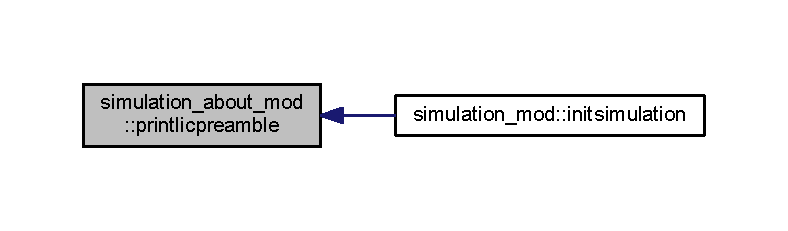
\includegraphics[width=350pt]{namespacesimulation__about__mod_ac436e98649d7488280cd176bbe765931_icgraph}
\end{center}
\end{figure}


\subsection{Variable Documentation}
\mbox{\Hypertarget{namespacesimulation__about__mod_a49c4e8683dee7c3a2cd52658879c6e38}\label{namespacesimulation__about__mod_a49c4e8683dee7c3a2cd52658879c6e38}} 
\index{simulation\+\_\+about\+\_\+mod@{simulation\+\_\+about\+\_\+mod}!author@{author}}
\index{author@{author}!simulation\+\_\+about\+\_\+mod@{simulation\+\_\+about\+\_\+mod}}
\subsubsection{\texorpdfstring{author}{author}}
{\footnotesize\ttfamily type(string) simulation\+\_\+about\+\_\+mod\+::author\hspace{0.3cm}{\ttfamily [private]}}



Definition at line 31 of file simulation\+\_\+about.\+f90.


\begin{DoxyCode}
31     \textcolor{keywordtype}{type}(string) :: author
\end{DoxyCode}
\mbox{\Hypertarget{namespacesimulation__about__mod_ad2ae0e434e2c6b0221094f181a538dc6}\label{namespacesimulation__about__mod_ad2ae0e434e2c6b0221094f181a538dc6}} 
\index{simulation\+\_\+about\+\_\+mod@{simulation\+\_\+about\+\_\+mod}!date@{date}}
\index{date@{date}!simulation\+\_\+about\+\_\+mod@{simulation\+\_\+about\+\_\+mod}}
\subsubsection{\texorpdfstring{date}{date}}
{\footnotesize\ttfamily type(string) simulation\+\_\+about\+\_\+mod\+::date\hspace{0.3cm}{\ttfamily [private]}}



Definition at line 32 of file simulation\+\_\+about.\+f90.


\begin{DoxyCode}
32     \textcolor{keywordtype}{type}(string) :: date
\end{DoxyCode}
\mbox{\Hypertarget{namespacesimulation__about__mod_aa52b892695e36d427843d6e035b37d36}\label{namespacesimulation__about__mod_aa52b892695e36d427843d6e035b37d36}} 
\index{simulation\+\_\+about\+\_\+mod@{simulation\+\_\+about\+\_\+mod}!version@{version}}
\index{version@{version}!simulation\+\_\+about\+\_\+mod@{simulation\+\_\+about\+\_\+mod}}
\subsubsection{\texorpdfstring{version}{version}}
{\footnotesize\ttfamily type(string) simulation\+\_\+about\+\_\+mod\+::version\hspace{0.3cm}{\ttfamily [private]}}



Definition at line 30 of file simulation\+\_\+about.\+f90.


\begin{DoxyCode}
30     \textcolor{keywordtype}{type}(string) :: version
\end{DoxyCode}

\hypertarget{namespacesimulation__globals__mod}{}\section{simulation\+\_\+globals\+\_\+mod Module Reference}
\label{namespacesimulation__globals__mod}\index{simulation\+\_\+globals\+\_\+mod@{simulation\+\_\+globals\+\_\+mod}}


Module to hold the simulation global parameter classes and their methods.  


\subsection*{Data Types}
\begin{DoxyCompactItemize}
\item 
type \hyperlink{structsimulation__globals__mod_1_1constants__t}{constants\+\_\+t}
\begin{DoxyCompactList}\small\item\em Case Constants class. \end{DoxyCompactList}\item 
type \hyperlink{structsimulation__globals__mod_1_1filenames__t}{filenames\+\_\+t}
\begin{DoxyCompactList}\small\item\em File names class. \end{DoxyCompactList}\item 
type \hyperlink{structsimulation__globals__mod_1_1globals__class}{globals\+\_\+class}
\begin{DoxyCompactList}\small\item\em Globals class -\/ This is a container for every global variable on the simulation. \end{DoxyCompactList}\item 
type \hyperlink{structsimulation__globals__mod_1_1parameters__t}{parameters\+\_\+t}
\item 
type \hyperlink{structsimulation__globals__mod_1_1simdefs__t}{simdefs\+\_\+t}
\begin{DoxyCompactList}\small\item\em Simulation definitions class. \end{DoxyCompactList}\end{DoxyCompactItemize}
\subsection*{Functions/\+Subroutines}
\begin{DoxyCompactItemize}
\item 
subroutine \hyperlink{namespacesimulation__globals__mod_ac2ac06271de377004c67b6ba2f3ed353}{setdefaults} (self)
\begin{DoxyCompactList}\small\item\em Globals default setting routine. \end{DoxyCompactList}\item 
subroutine \hyperlink{namespacesimulation__globals__mod_a8a05831d4c3e3eb5741d65978f6fcf61}{setparameter} (self, parmkey, parmvalue)
\begin{DoxyCompactList}\small\item\em Private parameter setting method. Builds the simulation parametric space from the input case file. \end{DoxyCompactList}\item 
subroutine \hyperlink{namespacesimulation__globals__mod_a41249abb5c33ef9e8bff448f0b3826fa}{check} (self)
\begin{DoxyCompactList}\small\item\em Parameter checking method. Checks if mandatory parameters were set. \end{DoxyCompactList}\item 
subroutine \hyperlink{namespacesimulation__globals__mod_a97c04d0289a9f2d004a9329cb7ab16f0}{printsimparameters} (self)
\begin{DoxyCompactList}\small\item\em Parameter printing method. \end{DoxyCompactList}\item 
subroutine \hyperlink{namespacesimulation__globals__mod_a68e871ed8e5d3930884e968c6fdafddc}{getintegratorname} (name, code)
\begin{DoxyCompactList}\small\item\em Routine to get integrator scheme name. \end{DoxyCompactList}\item 
subroutine \hyperlink{namespacesimulation__globals__mod_a9e92dfed4ef7388208adce768f064554}{setgravity} (self, grav)
\begin{DoxyCompactList}\small\item\em Gravity setting routine. \end{DoxyCompactList}\item 
subroutine \hyperlink{namespacesimulation__globals__mod_a64b1d91147c1cd5898fec8f23d56a65d}{setz0} (self, read\+\_\+z0)
\begin{DoxyCompactList}\small\item\em Z0 setting routine. \end{DoxyCompactList}\item 
subroutine \hyperlink{namespacesimulation__globals__mod_a68a87c39cf88bad353e28e367a721ed4}{setrho} (self, read\+\_\+rho)
\begin{DoxyCompactList}\small\item\em Rho\+\_\+\+Ref setting routine. \end{DoxyCompactList}\item 
subroutine \hyperlink{namespacesimulation__globals__mod_a20ba28d72a9bea823d9373a94f97026e}{printconstants} (self)
\begin{DoxyCompactList}\small\item\em Public constants printing routine. \end{DoxyCompactList}\item 
subroutine \hyperlink{namespacesimulation__globals__mod_acb8e3762572266b40a0deb166dded33a}{setdp} (self, read\+\_\+dp)
\begin{DoxyCompactList}\small\item\em Dp setting routine. \end{DoxyCompactList}\item 
subroutine \hyperlink{namespacesimulation__globals__mod_aecf75eeccef4eeae6d10ab26cf2dcfcf}{setdt} (self, read\+\_\+dt)
\begin{DoxyCompactList}\small\item\em Dt setting routine. \end{DoxyCompactList}\item 
subroutine \hyperlink{namespacesimulation__globals__mod_a412b0779703630189e2ea14e4b390864}{setboundingbox} (self, point\+\_\+, coords)
\begin{DoxyCompactList}\small\item\em Bounding box setting routine. \end{DoxyCompactList}\item 
subroutine \hyperlink{namespacesimulation__globals__mod_aa65b43534d2d2b6366a4ebc791194805}{setblocksize} (self, bsize)
\begin{DoxyCompactList}\small\item\em blocksize box setting routine. \end{DoxyCompactList}\item 
subroutine \hyperlink{namespacesimulation__globals__mod_ad331ccf019de7ed531e37c655600f90f}{printsimdefs} (self)
\begin{DoxyCompactList}\small\item\em Public simulation definitions printing routine. \end{DoxyCompactList}\end{DoxyCompactItemize}
\subsection*{Variables}
\begin{DoxyCompactItemize}
\item 
type(\hyperlink{structsimulation__globals__mod_1_1globals__class}{globals\+\_\+class}), public \hyperlink{namespacesimulation__globals__mod_a04123075b6de525703edb89697fc39e9}{globals}
\end{DoxyCompactItemize}


\subsection{Detailed Description}
Module to hold the simulation global parameter classes and their methods. 

\begin{DoxyAuthor}{Author}
Ricardo Birjukovs Canelas 
\end{DoxyAuthor}


\subsection{Function/\+Subroutine Documentation}
\mbox{\Hypertarget{namespacesimulation__globals__mod_a41249abb5c33ef9e8bff448f0b3826fa}\label{namespacesimulation__globals__mod_a41249abb5c33ef9e8bff448f0b3826fa}} 
\index{simulation\+\_\+globals\+\_\+mod@{simulation\+\_\+globals\+\_\+mod}!check@{check}}
\index{check@{check}!simulation\+\_\+globals\+\_\+mod@{simulation\+\_\+globals\+\_\+mod}}
\subsubsection{\texorpdfstring{check()}{check()}}
{\footnotesize\ttfamily subroutine simulation\+\_\+globals\+\_\+mod\+::check (\begin{DoxyParamCaption}\item[{class(\hyperlink{structsimulation__globals__mod_1_1parameters__t}{parameters\+\_\+t}), intent(inout)}]{self }\end{DoxyParamCaption})\hspace{0.3cm}{\ttfamily [private]}}



Parameter checking method. Checks if mandatory parameters were set. 

\begin{DoxyAuthor}{Author}
Ricardo Birjukovs Canelas -\/ M\+A\+R\+E\+T\+EC 
\end{DoxyAuthor}
\mbox{\Hypertarget{namespacesimulation__globals__mod_a68e871ed8e5d3930884e968c6fdafddc}\label{namespacesimulation__globals__mod_a68e871ed8e5d3930884e968c6fdafddc}} 
\index{simulation\+\_\+globals\+\_\+mod@{simulation\+\_\+globals\+\_\+mod}!getintegratorname@{getintegratorname}}
\index{getintegratorname@{getintegratorname}!simulation\+\_\+globals\+\_\+mod@{simulation\+\_\+globals\+\_\+mod}}
\subsubsection{\texorpdfstring{getintegratorname()}{getintegratorname()}}
{\footnotesize\ttfamily subroutine simulation\+\_\+globals\+\_\+mod\+::getintegratorname (\begin{DoxyParamCaption}\item[{type(string), intent(inout)}]{name,  }\item[{integer, intent(in)}]{code }\end{DoxyParamCaption})\hspace{0.3cm}{\ttfamily [private]}}



Routine to get integrator scheme name. 

\begin{DoxyAuthor}{Author}
Ricardo Birjukovs Canelas -\/ M\+A\+R\+E\+T\+EC 
\end{DoxyAuthor}
Here is the caller graph for this function\+:\nopagebreak
\begin{figure}[H]
\begin{center}
\leavevmode
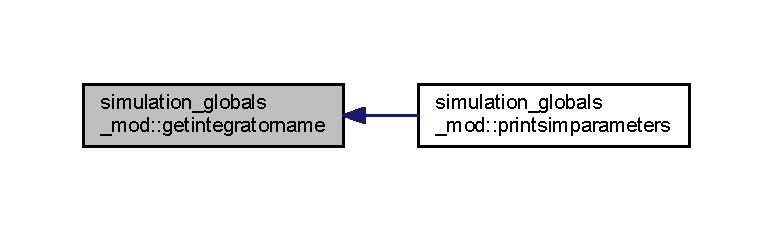
\includegraphics[width=350pt]{namespacesimulation__globals__mod_a68e871ed8e5d3930884e968c6fdafddc_icgraph}
\end{center}
\end{figure}
\mbox{\Hypertarget{namespacesimulation__globals__mod_a20ba28d72a9bea823d9373a94f97026e}\label{namespacesimulation__globals__mod_a20ba28d72a9bea823d9373a94f97026e}} 
\index{simulation\+\_\+globals\+\_\+mod@{simulation\+\_\+globals\+\_\+mod}!printconstants@{printconstants}}
\index{printconstants@{printconstants}!simulation\+\_\+globals\+\_\+mod@{simulation\+\_\+globals\+\_\+mod}}
\subsubsection{\texorpdfstring{printconstants()}{printconstants()}}
{\footnotesize\ttfamily subroutine simulation\+\_\+globals\+\_\+mod\+::printconstants (\begin{DoxyParamCaption}\item[{class(\hyperlink{structsimulation__globals__mod_1_1constants__t}{constants\+\_\+t}), intent(in)}]{self }\end{DoxyParamCaption})\hspace{0.3cm}{\ttfamily [private]}}



Public constants printing routine. 

\begin{DoxyAuthor}{Author}
Ricardo Birjukovs Canelas -\/ M\+A\+R\+E\+T\+EC 
\end{DoxyAuthor}
\mbox{\Hypertarget{namespacesimulation__globals__mod_ad331ccf019de7ed531e37c655600f90f}\label{namespacesimulation__globals__mod_ad331ccf019de7ed531e37c655600f90f}} 
\index{simulation\+\_\+globals\+\_\+mod@{simulation\+\_\+globals\+\_\+mod}!printsimdefs@{printsimdefs}}
\index{printsimdefs@{printsimdefs}!simulation\+\_\+globals\+\_\+mod@{simulation\+\_\+globals\+\_\+mod}}
\subsubsection{\texorpdfstring{printsimdefs()}{printsimdefs()}}
{\footnotesize\ttfamily subroutine simulation\+\_\+globals\+\_\+mod\+::printsimdefs (\begin{DoxyParamCaption}\item[{class(\hyperlink{structsimulation__globals__mod_1_1simdefs__t}{simdefs\+\_\+t}), intent(in)}]{self }\end{DoxyParamCaption})\hspace{0.3cm}{\ttfamily [private]}}



Public simulation definitions printing routine. 

\begin{DoxyAuthor}{Author}
Ricardo Birjukovs Canelas -\/ M\+A\+R\+E\+T\+EC 
\end{DoxyAuthor}
\mbox{\Hypertarget{namespacesimulation__globals__mod_a97c04d0289a9f2d004a9329cb7ab16f0}\label{namespacesimulation__globals__mod_a97c04d0289a9f2d004a9329cb7ab16f0}} 
\index{simulation\+\_\+globals\+\_\+mod@{simulation\+\_\+globals\+\_\+mod}!printsimparameters@{printsimparameters}}
\index{printsimparameters@{printsimparameters}!simulation\+\_\+globals\+\_\+mod@{simulation\+\_\+globals\+\_\+mod}}
\subsubsection{\texorpdfstring{printsimparameters()}{printsimparameters()}}
{\footnotesize\ttfamily subroutine simulation\+\_\+globals\+\_\+mod\+::printsimparameters (\begin{DoxyParamCaption}\item[{class(\hyperlink{structsimulation__globals__mod_1_1parameters__t}{parameters\+\_\+t}), intent(inout)}]{self }\end{DoxyParamCaption})\hspace{0.3cm}{\ttfamily [private]}}



Parameter printing method. 

\begin{DoxyAuthor}{Author}
Ricardo Birjukovs Canelas -\/ M\+A\+R\+E\+T\+EC 
\end{DoxyAuthor}
Here is the call graph for this function\+:\nopagebreak
\begin{figure}[H]
\begin{center}
\leavevmode
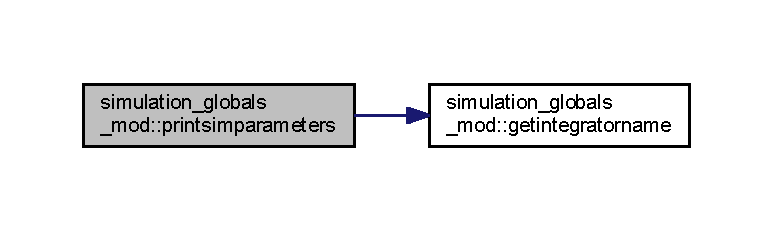
\includegraphics[width=350pt]{namespacesimulation__globals__mod_a97c04d0289a9f2d004a9329cb7ab16f0_cgraph}
\end{center}
\end{figure}
\mbox{\Hypertarget{namespacesimulation__globals__mod_aa65b43534d2d2b6366a4ebc791194805}\label{namespacesimulation__globals__mod_aa65b43534d2d2b6366a4ebc791194805}} 
\index{simulation\+\_\+globals\+\_\+mod@{simulation\+\_\+globals\+\_\+mod}!setblocksize@{setblocksize}}
\index{setblocksize@{setblocksize}!simulation\+\_\+globals\+\_\+mod@{simulation\+\_\+globals\+\_\+mod}}
\subsubsection{\texorpdfstring{setblocksize()}{setblocksize()}}
{\footnotesize\ttfamily subroutine simulation\+\_\+globals\+\_\+mod\+::setblocksize (\begin{DoxyParamCaption}\item[{class(\hyperlink{structsimulation__globals__mod_1_1simdefs__t}{simdefs\+\_\+t}), intent(inout)}]{self,  }\item[{type(vector)}]{bsize }\end{DoxyParamCaption})\hspace{0.3cm}{\ttfamily [private]}}



blocksize box setting routine. 

\begin{DoxyAuthor}{Author}
Ricardo Birjukovs Canelas -\/ M\+A\+R\+E\+T\+EC 
\end{DoxyAuthor}

\begin{DoxyParams}[1]{Parameters}
\mbox{\tt in}  & {\em bsize} & \\
\hline
\end{DoxyParams}
\mbox{\Hypertarget{namespacesimulation__globals__mod_a412b0779703630189e2ea14e4b390864}\label{namespacesimulation__globals__mod_a412b0779703630189e2ea14e4b390864}} 
\index{simulation\+\_\+globals\+\_\+mod@{simulation\+\_\+globals\+\_\+mod}!setboundingbox@{setboundingbox}}
\index{setboundingbox@{setboundingbox}!simulation\+\_\+globals\+\_\+mod@{simulation\+\_\+globals\+\_\+mod}}
\subsubsection{\texorpdfstring{setboundingbox()}{setboundingbox()}}
{\footnotesize\ttfamily subroutine simulation\+\_\+globals\+\_\+mod\+::setboundingbox (\begin{DoxyParamCaption}\item[{class(\hyperlink{structsimulation__globals__mod_1_1simdefs__t}{simdefs\+\_\+t}), intent(inout)}]{self,  }\item[{type(string), intent(in)}]{point\+\_\+,  }\item[{type(vector)}]{coords }\end{DoxyParamCaption})\hspace{0.3cm}{\ttfamily [private]}}



Bounding box setting routine. 

\begin{DoxyAuthor}{Author}
Ricardo Birjukovs Canelas -\/ M\+A\+R\+E\+T\+EC 
\end{DoxyAuthor}

\begin{DoxyParams}[1]{Parameters}
\mbox{\tt in}  & {\em point\+\_\+,coords} & \\
\hline
\end{DoxyParams}
\mbox{\Hypertarget{namespacesimulation__globals__mod_ac2ac06271de377004c67b6ba2f3ed353}\label{namespacesimulation__globals__mod_ac2ac06271de377004c67b6ba2f3ed353}} 
\index{simulation\+\_\+globals\+\_\+mod@{simulation\+\_\+globals\+\_\+mod}!setdefaults@{setdefaults}}
\index{setdefaults@{setdefaults}!simulation\+\_\+globals\+\_\+mod@{simulation\+\_\+globals\+\_\+mod}}
\subsubsection{\texorpdfstring{setdefaults()}{setdefaults()}}
{\footnotesize\ttfamily subroutine simulation\+\_\+globals\+\_\+mod\+::setdefaults (\begin{DoxyParamCaption}\item[{class(\hyperlink{structsimulation__globals__mod_1_1globals__class}{globals\+\_\+class}), intent(inout)}]{self }\end{DoxyParamCaption})\hspace{0.3cm}{\ttfamily [private]}}



Globals default setting routine. 

\begin{DoxyAuthor}{Author}
Ricardo Birjukovs Canelas -\/ M\+A\+R\+E\+T\+EC 
\end{DoxyAuthor}
\mbox{\Hypertarget{namespacesimulation__globals__mod_acb8e3762572266b40a0deb166dded33a}\label{namespacesimulation__globals__mod_acb8e3762572266b40a0deb166dded33a}} 
\index{simulation\+\_\+globals\+\_\+mod@{simulation\+\_\+globals\+\_\+mod}!setdp@{setdp}}
\index{setdp@{setdp}!simulation\+\_\+globals\+\_\+mod@{simulation\+\_\+globals\+\_\+mod}}
\subsubsection{\texorpdfstring{setdp()}{setdp()}}
{\footnotesize\ttfamily subroutine simulation\+\_\+globals\+\_\+mod\+::setdp (\begin{DoxyParamCaption}\item[{class(\hyperlink{structsimulation__globals__mod_1_1simdefs__t}{simdefs\+\_\+t}), intent(inout)}]{self,  }\item[{type(string), intent(in)}]{read\+\_\+dp }\end{DoxyParamCaption})\hspace{0.3cm}{\ttfamily [private]}}



Dp setting routine. 

\begin{DoxyAuthor}{Author}
Ricardo Birjukovs Canelas -\/ M\+A\+R\+E\+T\+EC 
\end{DoxyAuthor}

\begin{DoxyParams}[1]{Parameters}
\mbox{\tt in}  & {\em read\+\_\+dp} & \\
\hline
\end{DoxyParams}
\mbox{\Hypertarget{namespacesimulation__globals__mod_aecf75eeccef4eeae6d10ab26cf2dcfcf}\label{namespacesimulation__globals__mod_aecf75eeccef4eeae6d10ab26cf2dcfcf}} 
\index{simulation\+\_\+globals\+\_\+mod@{simulation\+\_\+globals\+\_\+mod}!setdt@{setdt}}
\index{setdt@{setdt}!simulation\+\_\+globals\+\_\+mod@{simulation\+\_\+globals\+\_\+mod}}
\subsubsection{\texorpdfstring{setdt()}{setdt()}}
{\footnotesize\ttfamily subroutine simulation\+\_\+globals\+\_\+mod\+::setdt (\begin{DoxyParamCaption}\item[{class(\hyperlink{structsimulation__globals__mod_1_1simdefs__t}{simdefs\+\_\+t}), intent(inout)}]{self,  }\item[{type(string), intent(in)}]{read\+\_\+dt }\end{DoxyParamCaption})\hspace{0.3cm}{\ttfamily [private]}}



Dt setting routine. 

\begin{DoxyAuthor}{Author}
Ricardo Birjukovs Canelas -\/ M\+A\+R\+E\+T\+EC 
\end{DoxyAuthor}

\begin{DoxyParams}[1]{Parameters}
\mbox{\tt in}  & {\em read\+\_\+dt} & \\
\hline
\end{DoxyParams}
\mbox{\Hypertarget{namespacesimulation__globals__mod_a9e92dfed4ef7388208adce768f064554}\label{namespacesimulation__globals__mod_a9e92dfed4ef7388208adce768f064554}} 
\index{simulation\+\_\+globals\+\_\+mod@{simulation\+\_\+globals\+\_\+mod}!setgravity@{setgravity}}
\index{setgravity@{setgravity}!simulation\+\_\+globals\+\_\+mod@{simulation\+\_\+globals\+\_\+mod}}
\subsubsection{\texorpdfstring{setgravity()}{setgravity()}}
{\footnotesize\ttfamily subroutine simulation\+\_\+globals\+\_\+mod\+::setgravity (\begin{DoxyParamCaption}\item[{class(\hyperlink{structsimulation__globals__mod_1_1constants__t}{constants\+\_\+t}), intent(inout)}]{self,  }\item[{type(vector), intent(in)}]{grav }\end{DoxyParamCaption})\hspace{0.3cm}{\ttfamily [private]}}



Gravity setting routine. 

\begin{DoxyAuthor}{Author}
Ricardo Birjukovs Canelas -\/ M\+A\+R\+E\+T\+EC 
\end{DoxyAuthor}

\begin{DoxyParams}[1]{Parameters}
\mbox{\tt in}  & {\em grav} & \\
\hline
\end{DoxyParams}
\mbox{\Hypertarget{namespacesimulation__globals__mod_a8a05831d4c3e3eb5741d65978f6fcf61}\label{namespacesimulation__globals__mod_a8a05831d4c3e3eb5741d65978f6fcf61}} 
\index{simulation\+\_\+globals\+\_\+mod@{simulation\+\_\+globals\+\_\+mod}!setparameter@{setparameter}}
\index{setparameter@{setparameter}!simulation\+\_\+globals\+\_\+mod@{simulation\+\_\+globals\+\_\+mod}}
\subsubsection{\texorpdfstring{setparameter()}{setparameter()}}
{\footnotesize\ttfamily subroutine simulation\+\_\+globals\+\_\+mod\+::setparameter (\begin{DoxyParamCaption}\item[{class(\hyperlink{structsimulation__globals__mod_1_1parameters__t}{parameters\+\_\+t}), intent(inout)}]{self,  }\item[{type(string), intent(in)}]{parmkey,  }\item[{type(string), intent(in)}]{parmvalue }\end{DoxyParamCaption})\hspace{0.3cm}{\ttfamily [private]}}



Private parameter setting method. Builds the simulation parametric space from the input case file. 

\begin{DoxyAuthor}{Author}
Ricardo Birjukovs Canelas -\/ M\+A\+R\+E\+T\+EC 
\end{DoxyAuthor}

\begin{DoxyParams}[1]{Parameters}
\mbox{\tt in}  & {\em parmkey,parmvalue} & \\
\hline
\end{DoxyParams}
\mbox{\Hypertarget{namespacesimulation__globals__mod_a68a87c39cf88bad353e28e367a721ed4}\label{namespacesimulation__globals__mod_a68a87c39cf88bad353e28e367a721ed4}} 
\index{simulation\+\_\+globals\+\_\+mod@{simulation\+\_\+globals\+\_\+mod}!setrho@{setrho}}
\index{setrho@{setrho}!simulation\+\_\+globals\+\_\+mod@{simulation\+\_\+globals\+\_\+mod}}
\subsubsection{\texorpdfstring{setrho()}{setrho()}}
{\footnotesize\ttfamily subroutine simulation\+\_\+globals\+\_\+mod\+::setrho (\begin{DoxyParamCaption}\item[{class(\hyperlink{structsimulation__globals__mod_1_1constants__t}{constants\+\_\+t}), intent(inout)}]{self,  }\item[{type(string), intent(in)}]{read\+\_\+rho }\end{DoxyParamCaption})\hspace{0.3cm}{\ttfamily [private]}}



Rho\+\_\+\+Ref setting routine. 

\begin{DoxyAuthor}{Author}
Ricardo Birjukovs Canelas -\/ M\+A\+R\+E\+T\+EC 
\end{DoxyAuthor}

\begin{DoxyParams}[1]{Parameters}
\mbox{\tt in}  & {\em read\+\_\+rho} & \\
\hline
\end{DoxyParams}
\mbox{\Hypertarget{namespacesimulation__globals__mod_a64b1d91147c1cd5898fec8f23d56a65d}\label{namespacesimulation__globals__mod_a64b1d91147c1cd5898fec8f23d56a65d}} 
\index{simulation\+\_\+globals\+\_\+mod@{simulation\+\_\+globals\+\_\+mod}!setz0@{setz0}}
\index{setz0@{setz0}!simulation\+\_\+globals\+\_\+mod@{simulation\+\_\+globals\+\_\+mod}}
\subsubsection{\texorpdfstring{setz0()}{setz0()}}
{\footnotesize\ttfamily subroutine simulation\+\_\+globals\+\_\+mod\+::setz0 (\begin{DoxyParamCaption}\item[{class(\hyperlink{structsimulation__globals__mod_1_1constants__t}{constants\+\_\+t}), intent(inout)}]{self,  }\item[{type(string), intent(in)}]{read\+\_\+z0 }\end{DoxyParamCaption})\hspace{0.3cm}{\ttfamily [private]}}



Z0 setting routine. 

\begin{DoxyAuthor}{Author}
Ricardo Birjukovs Canelas -\/ M\+A\+R\+E\+T\+EC 
\end{DoxyAuthor}

\begin{DoxyParams}[1]{Parameters}
\mbox{\tt in}  & {\em read\+\_\+z0} & \\
\hline
\end{DoxyParams}


\subsection{Variable Documentation}
\mbox{\Hypertarget{namespacesimulation__globals__mod_a04123075b6de525703edb89697fc39e9}\label{namespacesimulation__globals__mod_a04123075b6de525703edb89697fc39e9}} 
\index{simulation\+\_\+globals\+\_\+mod@{simulation\+\_\+globals\+\_\+mod}!globals@{globals}}
\index{globals@{globals}!simulation\+\_\+globals\+\_\+mod@{simulation\+\_\+globals\+\_\+mod}}
\subsubsection{\texorpdfstring{globals}{globals}}
{\footnotesize\ttfamily type(\hyperlink{structsimulation__globals__mod_1_1globals__class}{globals\+\_\+class}), public simulation\+\_\+globals\+\_\+mod\+::globals}


\hypertarget{namespacesimulation__initialize__mod}{}\section{simulation\+\_\+initialize\+\_\+mod Module Reference}
\label{namespacesimulation__initialize__mod}\index{simulation\+\_\+initialize\+\_\+mod@{simulation\+\_\+initialize\+\_\+mod}}


Module with the simulation initialization related definitions and methods. Has one public access routine that is incharge of building the simulation space from input files.  


\subsection*{Functions/\+Subroutines}
\begin{DoxyCompactItemize}
\item 
subroutine \mbox{\hyperlink{namespacesimulation__initialize__mod_a695ed61242e902d50bc40b83a6d11f65}{linkpropertysources}} (links\+Node)
\begin{DoxyCompactList}\small\item\em Private property xml parser routine. Reads the properties tab from the xml file and links these to the corresponding Source. \end{DoxyCompactList}\item 
subroutine \mbox{\hyperlink{namespacesimulation__initialize__mod_a7b30af4cf1a6ee74a4b2c6e8c9d1d98d}{init\+\_\+properties}} (case\+\_\+node)
\begin{DoxyCompactList}\small\item\em Private property xml parser routine. Reads the properties tab from the xml file and links these to the corresponding source. \end{DoxyCompactList}\item 
subroutine \mbox{\hyperlink{namespacesimulation__initialize__mod_ab6e350f9f537c9f62e8ba5aeb023d2a6}{read\+\_\+xml\+\_\+geometry}} (source, source\+\_\+detail, source\+\_\+shape)
\begin{DoxyCompactList}\small\item\em Private geometry xml parser routine. Reads a geometry from the xml depending on the geometry type of the node. \end{DoxyCompactList}\item 
subroutine \mbox{\hyperlink{namespacesimulation__initialize__mod_ae89df4e3074d9624a7db2bc015545d8d}{init\+\_\+sources}} (case\+\_\+node)
\begin{DoxyCompactList}\small\item\em Private source definitions parser routine. Builds the tracer sources from the input xml case file. \end{DoxyCompactList}\item 
subroutine \mbox{\hyperlink{namespacesimulation__initialize__mod_ae4a495136e5f02724a5cc456d5884281}{init\+\_\+simdefs}} (case\+\_\+node)
\begin{DoxyCompactList}\small\item\em Private simulation definitions parser routine. Builds the simulation geometric space from the input xml case file. \end{DoxyCompactList}\item 
subroutine \mbox{\hyperlink{namespacesimulation__initialize__mod_a97705c918360827c6fc76170b5eeb9bb}{init\+\_\+caseconstants}} (case\+\_\+node)
\begin{DoxyCompactList}\small\item\em Private case constant parser routine. Builds the simulation parametric space from the input xml case file. \end{DoxyCompactList}\item 
subroutine \mbox{\hyperlink{namespacesimulation__initialize__mod_a4ee29d81788bb77840a67af18784da66}{init\+\_\+parameters}} (execution\+\_\+node)
\begin{DoxyCompactList}\small\item\em Private parameter parser routine. Builds the simulation parametric space from the input xml case file. \end{DoxyCompactList}\item 
subroutine, public \mbox{\hyperlink{namespacesimulation__initialize__mod_aa596874d438807298121982eaa129d3a}{initfromxml}} (xmlfilename)
\begin{DoxyCompactList}\small\item\em Public xml parser routine. Builds the simulation space from the input xml case file. \end{DoxyCompactList}\end{DoxyCompactItemize}


\subsection{Detailed Description}
Module with the simulation initialization related definitions and methods. Has one public access routine that is incharge of building the simulation space from input files. 

\begin{DoxyAuthor}{Author}
Ricardo Birjukovs Canelas 
\end{DoxyAuthor}


\subsection{Function/\+Subroutine Documentation}
\mbox{\Hypertarget{namespacesimulation__initialize__mod_a97705c918360827c6fc76170b5eeb9bb}\label{namespacesimulation__initialize__mod_a97705c918360827c6fc76170b5eeb9bb}} 
\index{simulation\+\_\+initialize\+\_\+mod@{simulation\+\_\+initialize\+\_\+mod}!init\+\_\+caseconstants@{init\+\_\+caseconstants}}
\index{init\+\_\+caseconstants@{init\+\_\+caseconstants}!simulation\+\_\+initialize\+\_\+mod@{simulation\+\_\+initialize\+\_\+mod}}
\subsubsection{\texorpdfstring{init\+\_\+caseconstants()}{init\_caseconstants()}}
{\footnotesize\ttfamily subroutine simulation\+\_\+initialize\+\_\+mod\+::init\+\_\+caseconstants (\begin{DoxyParamCaption}\item[{type(node), intent(in), pointer}]{case\+\_\+node }\end{DoxyParamCaption})\hspace{0.3cm}{\ttfamily [private]}}



Private case constant parser routine. Builds the simulation parametric space from the input xml case file. 

\begin{DoxyAuthor}{Author}
Ricardo Birjukovs Canelas -\/ M\+A\+R\+E\+T\+EC 
\end{DoxyAuthor}

\begin{DoxyParams}[1]{Parameters}
\mbox{\tt in}  & {\em case\+\_\+node} & \\
\hline
\end{DoxyParams}


Definition at line 324 of file simulation\+\_\+initialize.\+f90.


\begin{DoxyCode}
324     \textcolor{keywordtype}{implicit none}
325     \textcolor{keywordtype}{type}(Node), \textcolor{keywordtype}{intent(in)}, \textcolor{keywordtype}{pointer} :: case\_node
326 
327     \textcolor{keywordtype}{type}(Node), \textcolor{keywordtype}{pointer} :: constants\_node
328     \textcolor{keywordtype}{type}(string) :: outext
329     \textcolor{keywordtype}{type}(string) :: tag, att\_name, att\_val
330     \textcolor{keywordtype}{type}(vector) :: coords
331     \textcolor{keywordtype}{logical} :: readflag
332 
333     outext=\textcolor{stringliteral}{'-->Reading case constants'}
334     \textcolor{keyword}{call }log%put(outext,.false.)
335 
336     tag=\textcolor{stringliteral}{"constantsdef"}    \textcolor{comment}{!the node we want}
337     \textcolor{keyword}{call }xmlreader%gotoNode(case\_node,constants\_node,tag,readflag,.false.)
338     \textcolor{keywordflow}{if} (readflag) \textcolor{keywordflow}{then} \textcolor{comment}{!if the node exists, since his one is not mandatory}
339         tag=\textcolor{stringliteral}{"Gravity"}
340         \textcolor{keyword}{call }xmlreader%getNodeVector(constants\_node,tag,coords,readflag,.false.)
341         \textcolor{keywordflow}{if} (readflag) \textcolor{keywordflow}{then}
342             \textcolor{keyword}{call }globals%Constants%setgravity(coords)
343 \textcolor{keywordflow}{        endif}
344         tag=\textcolor{stringliteral}{"Z0"}
345         att\_name=\textcolor{stringliteral}{"value"}
346         \textcolor{keyword}{call }xmlreader%getNodeAttribute(constants\_node, tag, att\_name, att\_val,readflag,.false.)
347         \textcolor{keywordflow}{if} (readflag) \textcolor{keywordflow}{then}
348             \textcolor{keyword}{call }globals%Constants%setz0(att\_val)
349 \textcolor{keywordflow}{        endif}
350         tag=\textcolor{stringliteral}{"Rho\_ref"}
351         att\_name=\textcolor{stringliteral}{"value"}
352         \textcolor{keyword}{call }xmlreader%getNodeAttribute(constants\_node, tag, att\_name, att\_val,readflag,.false.)
353         \textcolor{keywordflow}{if} (readflag) \textcolor{keywordflow}{then}
354             \textcolor{keyword}{call }globals%Constants%setrho(att\_val)
355 \textcolor{keywordflow}{        endif}
356 \textcolor{keywordflow}{    endif}
357     \textcolor{keyword}{call }globals%Constants%print()
358 
\end{DoxyCode}
Here is the caller graph for this function\+:\nopagebreak
\begin{figure}[H]
\begin{center}
\leavevmode
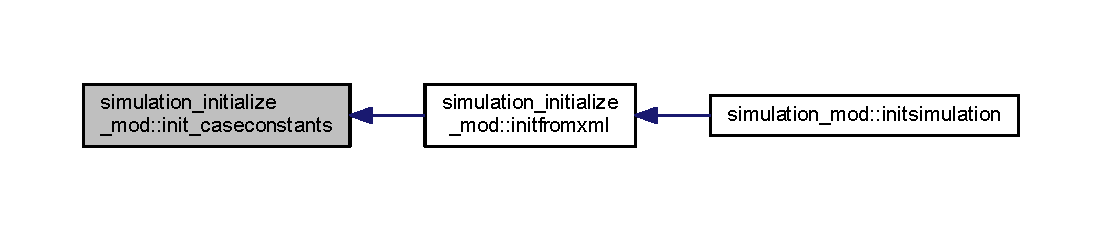
\includegraphics[width=350pt]{namespacesimulation__initialize__mod_a97705c918360827c6fc76170b5eeb9bb_icgraph}
\end{center}
\end{figure}
\mbox{\Hypertarget{namespacesimulation__initialize__mod_a4ee29d81788bb77840a67af18784da66}\label{namespacesimulation__initialize__mod_a4ee29d81788bb77840a67af18784da66}} 
\index{simulation\+\_\+initialize\+\_\+mod@{simulation\+\_\+initialize\+\_\+mod}!init\+\_\+parameters@{init\+\_\+parameters}}
\index{init\+\_\+parameters@{init\+\_\+parameters}!simulation\+\_\+initialize\+\_\+mod@{simulation\+\_\+initialize\+\_\+mod}}
\subsubsection{\texorpdfstring{init\+\_\+parameters()}{init\_parameters()}}
{\footnotesize\ttfamily subroutine simulation\+\_\+initialize\+\_\+mod\+::init\+\_\+parameters (\begin{DoxyParamCaption}\item[{type(node), intent(in), pointer}]{execution\+\_\+node }\end{DoxyParamCaption})\hspace{0.3cm}{\ttfamily [private]}}



Private parameter parser routine. Builds the simulation parametric space from the input xml case file. 

\begin{DoxyAuthor}{Author}
Ricardo Birjukovs Canelas -\/ M\+A\+R\+E\+T\+EC 
\end{DoxyAuthor}

\begin{DoxyParams}[1]{Parameters}
\mbox{\tt in}  & {\em execution\+\_\+node} & \\
\hline
\end{DoxyParams}


Definition at line 368 of file simulation\+\_\+initialize.\+f90.


\begin{DoxyCode}
368     \textcolor{keywordtype}{implicit none}
369     \textcolor{keywordtype}{type}(Node), \textcolor{keywordtype}{intent(in)}, \textcolor{keywordtype}{pointer} :: execution\_node
370 
371     \textcolor{keywordtype}{type}(string) :: outext
372     \textcolor{keywordtype}{type}(NodeList), \textcolor{keywordtype}{pointer} :: parameterList
373     \textcolor{keywordtype}{type}(Node), \textcolor{keywordtype}{pointer} :: parmt, parameters\_node
374     \textcolor{keywordtype}{integer} :: i
375     \textcolor{keywordtype}{type}(string) :: parmkey, parmvalue, tag, att\_name
376     \textcolor{keywordtype}{character(80)} :: parmkey\_char, parmvalue\_char
377 
378     outext=\textcolor{stringliteral}{'-->Reading case parameters'}
379     \textcolor{keyword}{call }log%put(outext,.false.)
380 
381     tag=\textcolor{stringliteral}{"parameters"}    \textcolor{comment}{!the node we want}
382     \textcolor{keyword}{call }xmlreader%gotoNode(execution\_node,parameters\_node,tag)
383     parameterlist => getelementsbytagname(parameters\_node, \textcolor{stringliteral}{"parameter"})       \textcolor{comment}{!searching for tags with the
       'parameter' name}
384     \textcolor{keywordflow}{do} i = 0, getlength(parameterlist) - 1                          \textcolor{comment}{!extracting parameter tags one by one}
385         parmt => item(parameterlist, i)
386         att\_name=\textcolor{stringliteral}{"key"}
387         \textcolor{keyword}{call }xmlreader%getLeafAttribute(parmt,att\_name,parmkey)
388         att\_name=\textcolor{stringliteral}{"value"}
389         \textcolor{keyword}{call }xmlreader%getLeafAttribute(parmt,att\_name,parmvalue)
390         \textcolor{keyword}{call }globals%Parameters%setparameter(parmkey,parmvalue)
391 \textcolor{keywordflow}{    enddo}
392     \textcolor{keyword}{call }globals%Parameters%check()
393     \textcolor{keyword}{call }globals%Parameters%print()
394 
\end{DoxyCode}
Here is the caller graph for this function\+:\nopagebreak
\begin{figure}[H]
\begin{center}
\leavevmode
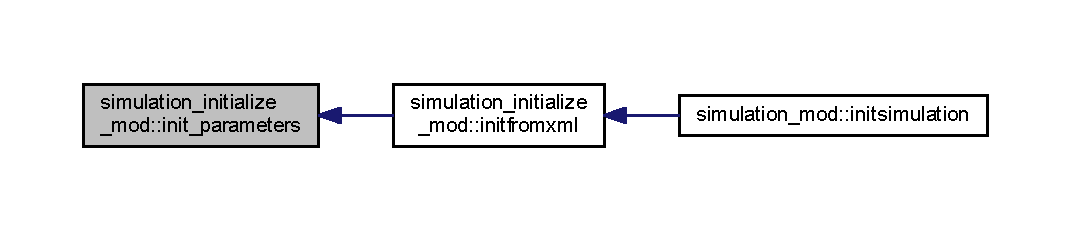
\includegraphics[width=350pt]{namespacesimulation__initialize__mod_a4ee29d81788bb77840a67af18784da66_icgraph}
\end{center}
\end{figure}
\mbox{\Hypertarget{namespacesimulation__initialize__mod_a7b30af4cf1a6ee74a4b2c6e8c9d1d98d}\label{namespacesimulation__initialize__mod_a7b30af4cf1a6ee74a4b2c6e8c9d1d98d}} 
\index{simulation\+\_\+initialize\+\_\+mod@{simulation\+\_\+initialize\+\_\+mod}!init\+\_\+properties@{init\+\_\+properties}}
\index{init\+\_\+properties@{init\+\_\+properties}!simulation\+\_\+initialize\+\_\+mod@{simulation\+\_\+initialize\+\_\+mod}}
\subsubsection{\texorpdfstring{init\+\_\+properties()}{init\_properties()}}
{\footnotesize\ttfamily subroutine simulation\+\_\+initialize\+\_\+mod\+::init\+\_\+properties (\begin{DoxyParamCaption}\item[{type(node), intent(in), pointer}]{case\+\_\+node }\end{DoxyParamCaption})\hspace{0.3cm}{\ttfamily [private]}}



Private property xml parser routine. Reads the properties tab from the xml file and links these to the corresponding source. 

\begin{DoxyAuthor}{Author}
Ricardo Birjukovs Canelas -\/ M\+A\+R\+E\+T\+EC 
\end{DoxyAuthor}

\begin{DoxyParams}[1]{Parameters}
\mbox{\tt in}  & {\em case\+\_\+node} & \\
\hline
\end{DoxyParams}


Definition at line 117 of file simulation\+\_\+initialize.\+f90.


\begin{DoxyCode}
117     \textcolor{keywordtype}{implicit none}
118     \textcolor{keywordtype}{type}(Node), \textcolor{keywordtype}{intent(in)}, \textcolor{keywordtype}{pointer} :: case\_node
119 
120     \textcolor{keywordtype}{type}(Node), \textcolor{keywordtype}{pointer} :: props\_node
121     \textcolor{keywordtype}{type}(string) :: outext
122     \textcolor{keywordtype}{type}(string) :: tag, att\_name
123 
124     tag=\textcolor{stringliteral}{"properties"}    \textcolor{comment}{!the node we want}
125     \textcolor{keyword}{call }xmlreader%gotoNode(case\_node,props\_node,tag,mandatory =.false.)
126     \textcolor{keywordflow}{if} (\textcolor{keyword}{associated}(props\_node)) \textcolor{keywordflow}{then}
127         tag=\textcolor{stringliteral}{"propertyfile"}
128         att\_name=\textcolor{stringliteral}{"name"}
129         \textcolor{keyword}{call }xmlreader%getNodeAttribute(props\_node, tag, att\_name, globals%Names%propsxmlfilename) \textcolor{comment}{!getting
       the file name from that tag}
130         outext=\textcolor{stringliteral}{'-->Properties to link to Sources found at '}//globals%Names%propsxmlfilename
131         \textcolor{keyword}{call }log%put(outext,.false.)
132         tag=\textcolor{stringliteral}{"links"}
133         \textcolor{keyword}{call }xmlreader%gotoNode(props\_node,props\_node,tag) \textcolor{comment}{!getting the links node}
134         \textcolor{keyword}{call }linkpropertysources(props\_node)          \textcolor{comment}{!calling the property linker}
135     \textcolor{keywordflow}{else}
136         outext=\textcolor{stringliteral}{'-->No properties to link to Sources, assuming pure Lagrangian tracers'}
137         \textcolor{keyword}{call }log%put(outext,.false.)
138 \textcolor{keywordflow}{    endif}
139 
\end{DoxyCode}
Here is the call graph for this function\+:\nopagebreak
\begin{figure}[H]
\begin{center}
\leavevmode
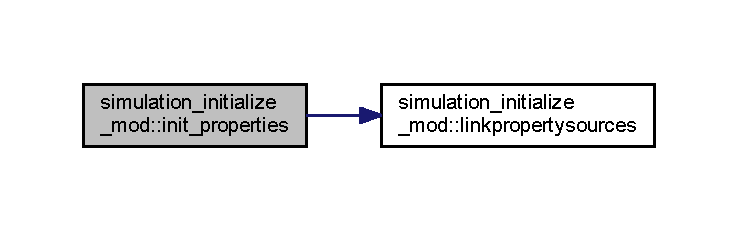
\includegraphics[width=350pt]{namespacesimulation__initialize__mod_a7b30af4cf1a6ee74a4b2c6e8c9d1d98d_cgraph}
\end{center}
\end{figure}
Here is the caller graph for this function\+:\nopagebreak
\begin{figure}[H]
\begin{center}
\leavevmode
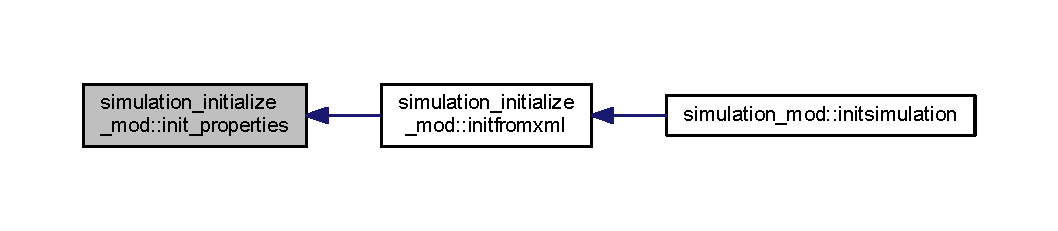
\includegraphics[width=350pt]{namespacesimulation__initialize__mod_a7b30af4cf1a6ee74a4b2c6e8c9d1d98d_icgraph}
\end{center}
\end{figure}
\mbox{\Hypertarget{namespacesimulation__initialize__mod_ae4a495136e5f02724a5cc456d5884281}\label{namespacesimulation__initialize__mod_ae4a495136e5f02724a5cc456d5884281}} 
\index{simulation\+\_\+initialize\+\_\+mod@{simulation\+\_\+initialize\+\_\+mod}!init\+\_\+simdefs@{init\+\_\+simdefs}}
\index{init\+\_\+simdefs@{init\+\_\+simdefs}!simulation\+\_\+initialize\+\_\+mod@{simulation\+\_\+initialize\+\_\+mod}}
\subsubsection{\texorpdfstring{init\+\_\+simdefs()}{init\_simdefs()}}
{\footnotesize\ttfamily subroutine simulation\+\_\+initialize\+\_\+mod\+::init\+\_\+simdefs (\begin{DoxyParamCaption}\item[{type(node), intent(in), pointer}]{case\+\_\+node }\end{DoxyParamCaption})\hspace{0.3cm}{\ttfamily [private]}}



Private simulation definitions parser routine. Builds the simulation geometric space from the input xml case file. 

\begin{DoxyAuthor}{Author}
Ricardo Birjukovs Canelas -\/ M\+A\+R\+E\+T\+EC 
\end{DoxyAuthor}

\begin{DoxyParams}[1]{Parameters}
\mbox{\tt in}  & {\em case\+\_\+node} & \\
\hline
\end{DoxyParams}


Definition at line 285 of file simulation\+\_\+initialize.\+f90.


\begin{DoxyCode}
285     \textcolor{keywordtype}{implicit none}
286     \textcolor{keywordtype}{type}(Node), \textcolor{keywordtype}{intent(in)}, \textcolor{keywordtype}{pointer} :: case\_node
287 
288     \textcolor{keywordtype}{type}(NodeList), \textcolor{keywordtype}{pointer} :: defsList
289     \textcolor{keywordtype}{type}(Node), \textcolor{keywordtype}{pointer} :: simdefs\_node
290     \textcolor{keywordtype}{type}(string) :: outext
291     \textcolor{keywordtype}{integer} :: i
292     \textcolor{keywordtype}{type}(string) :: pts(2), tag, att\_name, att\_val
293     \textcolor{keywordtype}{type}(vector) :: coords
294 
295     outext=\textcolor{stringliteral}{'-->Reading case simulation definitions'}
296     \textcolor{keyword}{call }log%put(outext,.false.)
297 
298     tag=\textcolor{stringliteral}{"simulationdefs"}    \textcolor{comment}{!the node we want}
299     \textcolor{keyword}{call }xmlreader%gotoNode(case\_node,simdefs\_node,tag)
300     tag=\textcolor{stringliteral}{"resolution"}
301     att\_name=\textcolor{stringliteral}{"dp"}
302     \textcolor{keyword}{call }xmlreader%getNodeAttribute(simdefs\_node, tag, att\_name, att\_val)
303     \textcolor{keyword}{call }globals%SimDefs%setdp(att\_val)
304     tag=\textcolor{stringliteral}{"timestep"}
305     att\_name=\textcolor{stringliteral}{"dt"}
306     \textcolor{keyword}{call }xmlreader%getNodeAttribute(simdefs\_node, tag, att\_name, att\_val)
307     \textcolor{keyword}{call }globals%SimDefs%setdt(att\_val)
308     pts=(/ \textcolor{stringliteral}{'pointmin'}, \textcolor{stringliteral}{'pointmax'}/) \textcolor{comment}{!strings to search for}
309     \textcolor{keywordflow}{do} i=1, \textcolor{keyword}{size}(pts)
310         \textcolor{keyword}{call }xmlreader%getNodeVector(simdefs\_node, pts(i), coords)
311         \textcolor{keyword}{call }globals%SimDefs%setboundingbox(pts(i), coords)
312 \textcolor{keywordflow}{    enddo}
313     \textcolor{keyword}{call }globals%SimDefs%print()
314 
\end{DoxyCode}
Here is the caller graph for this function\+:\nopagebreak
\begin{figure}[H]
\begin{center}
\leavevmode
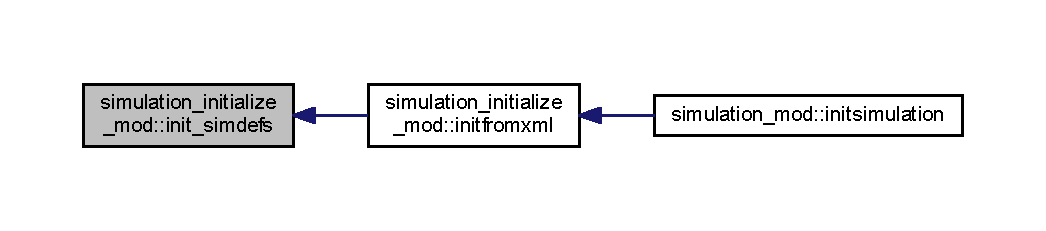
\includegraphics[width=350pt]{namespacesimulation__initialize__mod_ae4a495136e5f02724a5cc456d5884281_icgraph}
\end{center}
\end{figure}
\mbox{\Hypertarget{namespacesimulation__initialize__mod_ae89df4e3074d9624a7db2bc015545d8d}\label{namespacesimulation__initialize__mod_ae89df4e3074d9624a7db2bc015545d8d}} 
\index{simulation\+\_\+initialize\+\_\+mod@{simulation\+\_\+initialize\+\_\+mod}!init\+\_\+sources@{init\+\_\+sources}}
\index{init\+\_\+sources@{init\+\_\+sources}!simulation\+\_\+initialize\+\_\+mod@{simulation\+\_\+initialize\+\_\+mod}}
\subsubsection{\texorpdfstring{init\+\_\+sources()}{init\_sources()}}
{\footnotesize\ttfamily subroutine simulation\+\_\+initialize\+\_\+mod\+::init\+\_\+sources (\begin{DoxyParamCaption}\item[{type(node), intent(in), pointer}]{case\+\_\+node }\end{DoxyParamCaption})\hspace{0.3cm}{\ttfamily [private]}}



Private source definitions parser routine. Builds the tracer sources from the input xml case file. 

\begin{DoxyAuthor}{Author}
Ricardo Birjukovs Canelas -\/ M\+A\+R\+E\+T\+EC 
\end{DoxyAuthor}

\begin{DoxyParams}[1]{Parameters}
\mbox{\tt in}  & {\em case\+\_\+node} & \\
\hline
\end{DoxyParams}


Definition at line 192 of file simulation\+\_\+initialize.\+f90.


\begin{DoxyCode}
192     \textcolor{keywordtype}{implicit none}
193     \textcolor{keywordtype}{type}(Node), \textcolor{keywordtype}{intent(in)}, \textcolor{keywordtype}{pointer} :: case\_node
194 
195     \textcolor{keywordtype}{type}(string) :: outext
196     \textcolor{keywordtype}{type}(NodeList), \textcolor{keywordtype}{pointer} :: sourceList
197     \textcolor{keywordtype}{type}(NodeList), \textcolor{keywordtype}{pointer} :: sourceChildren
198     \textcolor{keywordtype}{type}(Node), \textcolor{keywordtype}{pointer} :: sourcedef
199     \textcolor{keywordtype}{type}(Node), \textcolor{keywordtype}{pointer} :: source\_node
200     \textcolor{keywordtype}{type}(Node), \textcolor{keywordtype}{pointer} :: source\_detail
201     \textcolor{keywordtype}{integer} :: i, j
202     \textcolor{keywordtype}{logical} :: readflag
203     \textcolor{comment}{!source vars}
204     \textcolor{keywordtype}{integer} :: id
205     \textcolor{keywordtype}{type}(string) :: name, source\_geometry, tag, att\_name, att\_val
206     \textcolor{keywordtype}{real(prec)} :: emitting\_rate, start, finish
207     \textcolor{keywordtype}{class}(shape), \textcolor{keywordtype}{allocatable} :: source\_shape
208 
209     outext=\textcolor{stringliteral}{'-->Reading case Sources'}
210     \textcolor{keyword}{call }log%put(outext,.false.)
211 
212     tag=\textcolor{stringliteral}{"sourcedef"}    \textcolor{comment}{!the node we want}
213     \textcolor{keyword}{call }xmlreader%gotoNode(case\_node,sourcedef,tag)
214     sourcelist => getelementsbytagname(sourcedef, \textcolor{stringliteral}{"source"})
215 
216     \textcolor{comment}{!allocating the temporary source objects}
217     \textcolor{keyword}{call }tempsources%initialize(getlength(sourcelist))
218 
219     \textcolor{keywordflow}{do} j = 0, getlength(sourcelist) - 1
220         source\_node => item(sourcelist,j)
221         tag=\textcolor{stringliteral}{"setsource"}
222         att\_name=\textcolor{stringliteral}{"id"}
223         \textcolor{keyword}{call }xmlreader%getNodeAttribute(source\_node, tag, att\_name, att\_val)
224         id=att\_val%to\_number(kind=1\_i1p)
225         att\_name=\textcolor{stringliteral}{"name"}
226         \textcolor{keyword}{call }xmlreader%getNodeAttribute(source\_node, tag, att\_name, name)
227         tag=\textcolor{stringliteral}{"rate"}
228         att\_name=\textcolor{stringliteral}{"value"}
229         \textcolor{keyword}{call }xmlreader%getNodeAttribute(source\_node, tag, att\_name, att\_val)
230         emitting\_rate = att\_val%to\_number(kind=1.\_r4p)
231         tag=\textcolor{stringliteral}{"active"}
232         att\_name=\textcolor{stringliteral}{"start"}
233         \textcolor{keyword}{call }xmlreader%getNodeAttribute(source\_node, tag, att\_name, att\_val,readflag,.false.)
234         \textcolor{keywordflow}{if} (readflag) \textcolor{keywordflow}{then}
235             start = att\_val%to\_number(kind=1.\_r4p)
236         \textcolor{keywordflow}{else}
237             start = 0.0
238 \textcolor{keywordflow}{        endif}
239         att\_name=\textcolor{stringliteral}{"end"}
240         \textcolor{keyword}{call }xmlreader%getNodeAttribute(source\_node, tag, att\_name, att\_val,readflag,.false.)
241         \textcolor{keywordflow}{if} (readflag.and.att\_val%is\_number()) \textcolor{keywordflow}{then}
242             finish = att\_val%to\_number(kind=1.\_r4p)
243         \textcolor{keywordflow}{else}
244             finish = globals%Parameters%TimeMax
245 \textcolor{keywordflow}{        endif}
246         \textcolor{comment}{!now we need to find out the geometry of the source and read accordingly}
247         sourcechildren => getchildnodes(source\_node) \textcolor{comment}{!getting all of the nodes bellow the main source node
       (all of it's private info)}
248         \textcolor{keywordflow}{do} i=0, getlength(sourcechildren)-1
249             source\_detail => item(sourcechildren,i) \textcolor{comment}{!grabing a node}
250             source\_geometry = getlocalname(source\_detail)  \textcolor{comment}{!finding its name}
251             \textcolor{keywordflow}{if} (geometry%inlist(source\_geometry)) \textcolor{keywordflow}{then}  \textcolor{comment}{!if the node is a valid geometry name}
252                 \textcolor{keywordflow}{select case} (source\_geometry%chars())
253                 \textcolor{keywordflow}{case} (\textcolor{stringliteral}{'point'})
254                     \textcolor{keyword}{allocate}(point::source\_shape)
255                 \textcolor{keywordflow}{case} (\textcolor{stringliteral}{'sphere'})
256                     \textcolor{keyword}{allocate}(sphere::source\_shape)
257                 \textcolor{keywordflow}{case} (\textcolor{stringliteral}{'box'})
258                     \textcolor{keyword}{allocate}(box::source\_shape)
259                 \textcolor{keywordflow}{case} (\textcolor{stringliteral}{'line'})
260                     \textcolor{keyword}{allocate}(line::source\_shape)
261 \textcolor{keywordflow}{                    case default}
262                     outext=\textcolor{stringliteral}{'[init\_sources]: unexpected type for geometry object!'}
263                     \textcolor{keyword}{call }log%put(outext)
264                     stop
265 \textcolor{keywordflow}{                end select}
266                 \textcolor{keyword}{call }read\_xml\_geometry(source\_node,source\_detail,source\_shape)
267                 \textcolor{keywordflow}{exit}
268 \textcolor{keywordflow}{            endif}
269 \textcolor{keywordflow}{        enddo}
270         \textcolor{comment}{!initializing Source j}
271         \textcolor{keyword}{call }tempsources%src(j+1)%initialize(id,name,emitting\_rate,start,finish,source\_geometry,
      source\_shape)
272 
273         \textcolor{keyword}{deallocate}(source\_shape)
274 \textcolor{keywordflow}{    enddo}
275 
\end{DoxyCode}
Here is the call graph for this function\+:\nopagebreak
\begin{figure}[H]
\begin{center}
\leavevmode
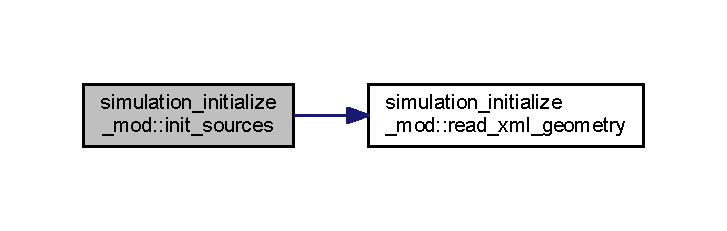
\includegraphics[width=349pt]{namespacesimulation__initialize__mod_ae89df4e3074d9624a7db2bc015545d8d_cgraph}
\end{center}
\end{figure}
Here is the caller graph for this function\+:\nopagebreak
\begin{figure}[H]
\begin{center}
\leavevmode
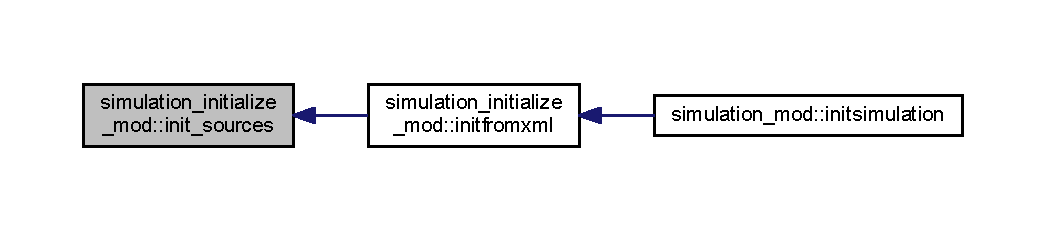
\includegraphics[width=350pt]{namespacesimulation__initialize__mod_ae89df4e3074d9624a7db2bc015545d8d_icgraph}
\end{center}
\end{figure}
\mbox{\Hypertarget{namespacesimulation__initialize__mod_aa596874d438807298121982eaa129d3a}\label{namespacesimulation__initialize__mod_aa596874d438807298121982eaa129d3a}} 
\index{simulation\+\_\+initialize\+\_\+mod@{simulation\+\_\+initialize\+\_\+mod}!initfromxml@{initfromxml}}
\index{initfromxml@{initfromxml}!simulation\+\_\+initialize\+\_\+mod@{simulation\+\_\+initialize\+\_\+mod}}
\subsubsection{\texorpdfstring{initfromxml()}{initfromxml()}}
{\footnotesize\ttfamily subroutine, public simulation\+\_\+initialize\+\_\+mod\+::initfromxml (\begin{DoxyParamCaption}\item[{type(string), intent(in)}]{xmlfilename }\end{DoxyParamCaption})}



Public xml parser routine. Builds the simulation space from the input xml case file. 

\begin{DoxyAuthor}{Author}
Ricardo Birjukovs Canelas -\/ M\+A\+R\+E\+T\+EC 
\end{DoxyAuthor}

\begin{DoxyParams}[1]{Parameters}
\mbox{\tt in}  & {\em xmlfilename} & \\
\hline
\mbox{\tt in}  & {\em xmlfilename} & .xml file name \\
\hline
\end{DoxyParams}


Definition at line 404 of file simulation\+\_\+initialize.\+f90.


\begin{DoxyCode}
404     \textcolor{keywordtype}{implicit none}
405     \textcolor{keywordtype}{type}(string), \textcolor{keywordtype}{intent(in)} :: xmlfilename
406     \textcolor{keywordtype}{type}(string) :: outext, tag
407     \textcolor{keywordtype}{type}(Node), \textcolor{keywordtype}{pointer} :: xmldoc
408     \textcolor{keywordtype}{type}(Node), \textcolor{keywordtype}{pointer} :: case\_node
409     \textcolor{keywordtype}{type}(Node), \textcolor{keywordtype}{pointer} :: execution\_node
410 
411     \textcolor{keyword}{call }xmlreader%getFile(xmldoc,xmlfilename)
412     globals%Names%mainxmlfilename = xmlfilename
413     globals%Names%casename = xmlfilename%basename(extension=\textcolor{stringliteral}{'.xml'})
414     outext=\textcolor{stringliteral}{'->Case name is '}//globals%Names%casename
415     \textcolor{keyword}{call }log%put(outext)
416 
417     tag=\textcolor{stringliteral}{"case"}          \textcolor{comment}{!base document node}
418     \textcolor{keyword}{call }xmlreader%gotoNode(xmldoc,execution\_node,tag)
419     tag=\textcolor{stringliteral}{"execution"}     \textcolor{comment}{!finding execution node}
420     \textcolor{keyword}{call }xmlreader%gotoNode(execution\_node,execution\_node,tag)
421     tag=\textcolor{stringliteral}{"case"}          \textcolor{comment}{!base document node}
422     \textcolor{keyword}{call }xmlreader%gotoNode(xmldoc,case\_node,tag)
423     tag=\textcolor{stringliteral}{"casedef"}     \textcolor{comment}{!finding execution node}
424     \textcolor{keyword}{call }xmlreader%gotoNode(case\_node,case\_node,tag)
425 
426     \textcolor{comment}{! building the simulation basic structures according to the case definition file}
427     \textcolor{comment}{! every other structure in the simulation is built from these, i.e., not defined by the user directly}
428     \textcolor{keyword}{call }init\_parameters(execution\_node)
429     \textcolor{keyword}{call }init\_caseconstants(case\_node)
430     \textcolor{keyword}{call }init\_simdefs(case\_node)
431     \textcolor{keyword}{call }init\_sources(case\_node)
432     \textcolor{keyword}{call }init\_properties(case\_node)
433 
434     \textcolor{keyword}{call }xmlreader%closeFile(xmldoc)
435 
\end{DoxyCode}
Here is the call graph for this function\+:\nopagebreak
\begin{figure}[H]
\begin{center}
\leavevmode
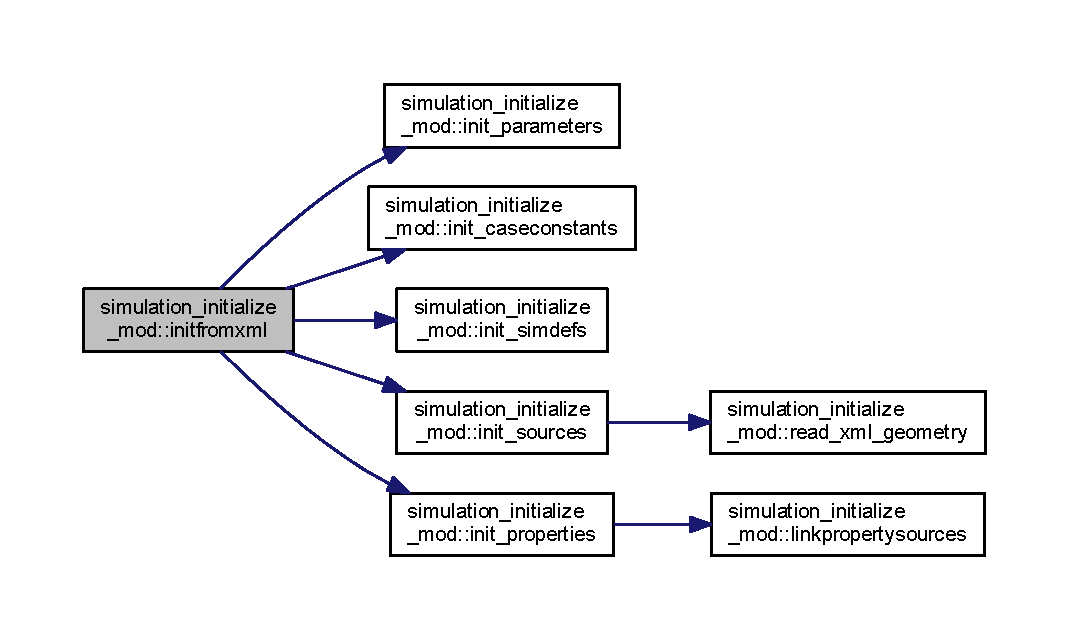
\includegraphics[width=350pt]{namespacesimulation__initialize__mod_aa596874d438807298121982eaa129d3a_cgraph}
\end{center}
\end{figure}
Here is the caller graph for this function\+:\nopagebreak
\begin{figure}[H]
\begin{center}
\leavevmode
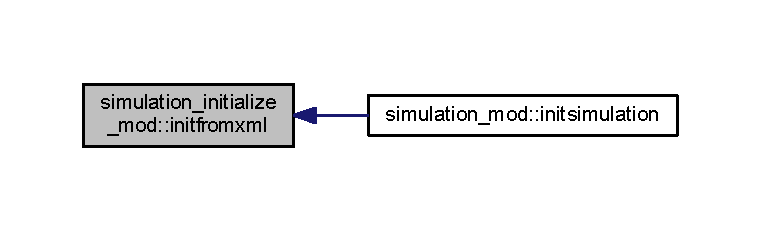
\includegraphics[width=350pt]{namespacesimulation__initialize__mod_aa596874d438807298121982eaa129d3a_icgraph}
\end{center}
\end{figure}
\mbox{\Hypertarget{namespacesimulation__initialize__mod_a695ed61242e902d50bc40b83a6d11f65}\label{namespacesimulation__initialize__mod_a695ed61242e902d50bc40b83a6d11f65}} 
\index{simulation\+\_\+initialize\+\_\+mod@{simulation\+\_\+initialize\+\_\+mod}!linkpropertysources@{linkpropertysources}}
\index{linkpropertysources@{linkpropertysources}!simulation\+\_\+initialize\+\_\+mod@{simulation\+\_\+initialize\+\_\+mod}}
\subsubsection{\texorpdfstring{linkpropertysources()}{linkpropertysources()}}
{\footnotesize\ttfamily subroutine simulation\+\_\+initialize\+\_\+mod\+::linkpropertysources (\begin{DoxyParamCaption}\item[{type(node), intent(in), pointer}]{links\+Node }\end{DoxyParamCaption})\hspace{0.3cm}{\ttfamily [private]}}



Private property xml parser routine. Reads the properties tab from the xml file and links these to the corresponding Source. 

\begin{DoxyAuthor}{Author}
Ricardo Birjukovs Canelas -\/ M\+A\+R\+E\+T\+EC 
\end{DoxyAuthor}

\begin{DoxyParams}[1]{Parameters}
\mbox{\tt in}  & {\em links\+Node} & \\
\hline
\end{DoxyParams}


Definition at line 47 of file simulation\+\_\+initialize.\+f90.


\begin{DoxyCode}
47     \textcolor{keywordtype}{implicit none}
48     \textcolor{keywordtype}{type}(Node), \textcolor{keywordtype}{intent(in)}, \textcolor{keywordtype}{pointer} :: linksNode
49 
50     \textcolor{keywordtype}{type}(NodeList), \textcolor{keywordtype}{pointer} :: linkList
51     \textcolor{keywordtype}{type}(Node), \textcolor{keywordtype}{pointer} :: anode
52     \textcolor{keywordtype}{type}(Node), \textcolor{keywordtype}{pointer} :: xmlProps
53     \textcolor{keywordtype}{type}(string) :: xmlfilename, outext
54     \textcolor{keywordtype}{integer} :: i, p
55     \textcolor{keywordtype}{type}(string) :: att\_name, att\_val, tag
56     \textcolor{keywordtype}{type}(string) :: sourceid, sourcetype, sourceprop
57 
58     linklist => getelementsbytagname(linksnode, \textcolor{stringliteral}{"link"})
59     \textcolor{keywordflow}{do} i = 0, getlength(linklist) - 1
60         anode => item(linklist,i)
61         att\_name=\textcolor{stringliteral}{"source"}
62         \textcolor{keyword}{call }xmlreader%getLeafAttribute(anode,att\_name,sourceid)
63         att\_name=\textcolor{stringliteral}{"type"}
64         \textcolor{keyword}{call }xmlreader%getLeafAttribute(anode,att\_name,sourcetype)
65         att\_name=\textcolor{stringliteral}{"property"}
66         \textcolor{keyword}{call }xmlreader%getLeafAttribute(anode,att\_name,sourceprop)
67         \textcolor{comment}{!find the source and save the type and property name}
68         \textcolor{keyword}{call }tempsources%setPropertyNames(sourceid,sourcetype,sourceprop)
69 \textcolor{keywordflow}{    enddo}
70 
71     \textcolor{comment}{!parse the properties file}
72     xmlfilename = globals%Names%propsxmlfilename
73     \textcolor{keyword}{call }xmlreader%getFile(xmlprops,xmlfilename)
74 
75     \textcolor{comment}{!Go to the materials node}
76     tag = \textcolor{stringliteral}{"materials"}
77     \textcolor{keyword}{call }xmlreader%gotoNode(xmlprops,xmlprops,tag)
78 
79     \textcolor{comment}{!find and set the actual atributes of the properties}
80     att\_name=\textcolor{stringliteral}{"value"}
81     \textcolor{keywordflow}{do} i = 1, \textcolor{keyword}{size}(tempsources%src)
82         tag = tempsources%src(i)%prop%property\_type
83         \textcolor{keywordflow}{if} (tag .ne. \textcolor{stringliteral}{'base'}) \textcolor{keywordflow}{then}
84             \textcolor{keyword}{call }xmlreader%gotoNode(xmlprops,anode,tag) \textcolor{comment}{!finding the material type node}
85             tag = tempsources%src(i)%prop%property\_name
86             \textcolor{keyword}{call }xmlreader%gotoNode(anode,anode,tag)     \textcolor{comment}{!finding the actual material node}
87             \textcolor{keywordflow}{do} p = 1, \textcolor{keyword}{size}(globals%SrcProp%baselist)
88                 \textcolor{keyword}{call }xmlreader%getNodeAttribute(anode, globals%SrcProp%baselist(p), att\_name, att\_val)
89                 \textcolor{keyword}{call }tempsources%src(i)%setPropertyAtributes(globals%SrcProp%baselist(p), att\_val)
90 \textcolor{keywordflow}{            end do}
91             \textcolor{keywordflow}{if} (tempsources%src(i)%isParticulate()) \textcolor{keywordflow}{then}
92                 \textcolor{keywordflow}{do} p = 1, \textcolor{keyword}{size}(globals%SrcProp%particulatelist)
93                     \textcolor{keyword}{call }xmlreader%getNodeAttribute(anode, globals%SrcProp%particulatelist(p), att\_name, 
      att\_val)
94                     \textcolor{keyword}{call }tempsources%src(i)%setPropertyAtributes(globals%SrcProp%particulatelist(p), 
      att\_val)
95 \textcolor{keywordflow}{                end do}
96 \textcolor{keywordflow}{            end if}
97             \textcolor{comment}{!Run integrety check on the properties to see if Source is well defined}
98             \textcolor{keyword}{call }tempsources%src(i)%check()
99 \textcolor{keywordflow}{        end if}
100 \textcolor{keywordflow}{    end do}
101     outext=\textcolor{stringliteral}{'-->Sources properties are set'}
102     \textcolor{keyword}{call }log%put(outext,.false.)
103 
104     \textcolor{keyword}{call }xmlreader%closeFile(xmlprops)
105 
\end{DoxyCode}
Here is the caller graph for this function\+:\nopagebreak
\begin{figure}[H]
\begin{center}
\leavevmode
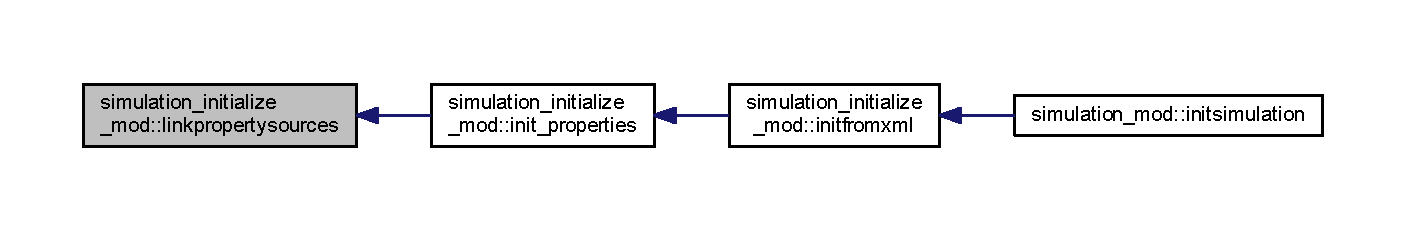
\includegraphics[width=350pt]{namespacesimulation__initialize__mod_a695ed61242e902d50bc40b83a6d11f65_icgraph}
\end{center}
\end{figure}
\mbox{\Hypertarget{namespacesimulation__initialize__mod_ab6e350f9f537c9f62e8ba5aeb023d2a6}\label{namespacesimulation__initialize__mod_ab6e350f9f537c9f62e8ba5aeb023d2a6}} 
\index{simulation\+\_\+initialize\+\_\+mod@{simulation\+\_\+initialize\+\_\+mod}!read\+\_\+xml\+\_\+geometry@{read\+\_\+xml\+\_\+geometry}}
\index{read\+\_\+xml\+\_\+geometry@{read\+\_\+xml\+\_\+geometry}!simulation\+\_\+initialize\+\_\+mod@{simulation\+\_\+initialize\+\_\+mod}}
\subsubsection{\texorpdfstring{read\+\_\+xml\+\_\+geometry()}{read\_xml\_geometry()}}
{\footnotesize\ttfamily subroutine simulation\+\_\+initialize\+\_\+mod\+::read\+\_\+xml\+\_\+geometry (\begin{DoxyParamCaption}\item[{type(node), intent(in), pointer}]{source,  }\item[{type(node), intent(in), pointer}]{source\+\_\+detail,  }\item[{class(\mbox{\hyperlink{structgeometry__mod_1_1shape}{shape}}), intent(inout)}]{source\+\_\+shape }\end{DoxyParamCaption})\hspace{0.3cm}{\ttfamily [private]}}



Private geometry xml parser routine. Reads a geometry from the xml depending on the geometry type of the node. 

\begin{DoxyAuthor}{Author}
Ricardo Birjukovs Canelas -\/ M\+A\+R\+E\+T\+EC 
\end{DoxyAuthor}

\begin{DoxyParams}[1]{Parameters}
\mbox{\tt in}  & {\em source,source\+\_\+detail,source\+\_\+shape} & \\
\hline
\mbox{\tt in}  & {\em source} & Working xml node\\
\hline
\mbox{\tt in}  & {\em source\+\_\+detail} & Working xml node details\\
\hline
\mbox{\tt in,out}  & {\em source\+\_\+shape} & Geometrical object to fill \\
\hline
\end{DoxyParams}


Definition at line 150 of file simulation\+\_\+initialize.\+f90.


\begin{DoxyCode}
150     \textcolor{keywordtype}{implicit none}
151     \textcolor{keywordtype}{type}(Node), \textcolor{keywordtype}{intent(in)}, \textcolor{keywordtype}{pointer} :: source
152     \textcolor{keywordtype}{type}(Node), \textcolor{keywordtype}{intent(in)}, \textcolor{keywordtype}{pointer} :: source\_detail
153     \textcolor{keywordtype}{class}(shape), \textcolor{keywordtype}{intent(inout)} :: source\_shape
154     \textcolor{keywordtype}{type}(string) :: outext
155     \textcolor{keywordtype}{type}(string) :: tag
156 
157     \textcolor{keywordflow}{select type} (source\_shape)
158 \textcolor{keywordflow}{    type is} (shape)
159         \textcolor{comment}{!nothing to do}
160 \textcolor{keywordflow}{    class is} (box)
161         tag=\textcolor{stringliteral}{'point'}
162         \textcolor{keyword}{call }xmlreader%getNodeVector(source\_detail,tag,source\_shape%pt)
163         tag=\textcolor{stringliteral}{'size'}
164         \textcolor{keyword}{call }xmlreader%getNodeVector(source\_detail,tag,source\_shape%size)
165 \textcolor{keywordflow}{    class is} (point)
166         tag=\textcolor{stringliteral}{'point'}
167         \textcolor{keyword}{call }xmlreader%getNodeVector(source,tag,source\_shape%pt)
168 \textcolor{keywordflow}{    class is} (line)
169         tag=\textcolor{stringliteral}{'pointa'}
170         \textcolor{keyword}{call }xmlreader%getNodeVector(source\_detail,tag,source\_shape%pt)
171         tag=\textcolor{stringliteral}{'pointb'}
172         \textcolor{keyword}{call }xmlreader%getNodeVector(source\_detail,tag,source\_shape%last)
173 \textcolor{keywordflow}{    class is} (sphere)
174         tag=\textcolor{stringliteral}{'point'}
175         \textcolor{keyword}{call }xmlreader%getNodeVector(source\_detail,tag,source\_shape%pt)
176         \textcolor{keyword}{call }extractdataattribute(source\_detail, \textcolor{stringliteral}{"radius"}, source\_shape%radius)
177 \textcolor{keywordflow}{        class default}
178         outext=\textcolor{stringliteral}{'[read\_xml\_geometry]: unexpected type for geometry object!'}
179         \textcolor{keyword}{call }log%put(outext)
180         stop
181 \textcolor{keywordflow}{    end select}
182 
\end{DoxyCode}
Here is the caller graph for this function\+:\nopagebreak
\begin{figure}[H]
\begin{center}
\leavevmode
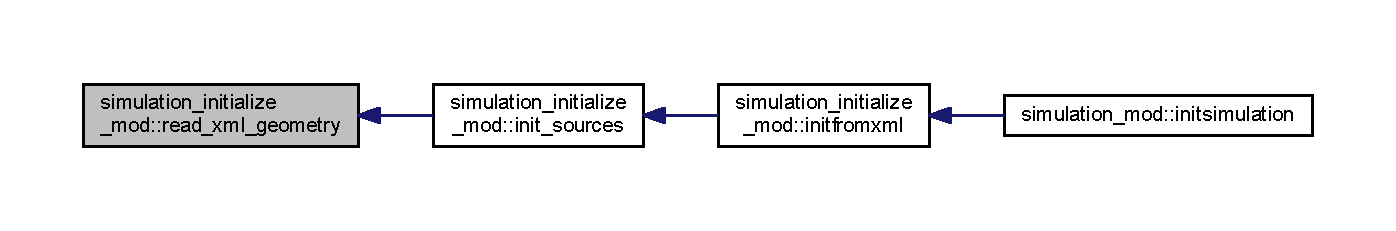
\includegraphics[width=350pt]{namespacesimulation__initialize__mod_ab6e350f9f537c9f62e8ba5aeb023d2a6_icgraph}
\end{center}
\end{figure}

\hypertarget{namespacesimulation__logger__mod}{}\section{simulation\+\_\+logger\+\_\+mod Module Reference}
\label{namespacesimulation__logger__mod}\index{simulation\+\_\+logger\+\_\+mod@{simulation\+\_\+logger\+\_\+mod}}


Module to hold all the simulation logger related definitions and methods.  


\subsection*{Data Types}
\begin{DoxyCompactItemize}
\item 
type \hyperlink{structsimulation__logger__mod_1_1logger__class}{logger\+\_\+class}
\end{DoxyCompactItemize}
\subsection*{Functions/\+Subroutines}
\begin{DoxyCompactItemize}
\item 
subroutine \hyperlink{namespacesimulation__logger__mod_abf603e657da9104a8060ab53c72f0aca}{initlog} (self, outpath)
\begin{DoxyCompactList}\small\item\em Log file initizalization routine. \end{DoxyCompactList}\item 
subroutine \hyperlink{namespacesimulation__logger__mod_aa6d1aaea74403186da0f98afb74ecebe}{closelog} (self)
\begin{DoxyCompactList}\small\item\em Log file closure routine. \end{DoxyCompactList}\item 
subroutine \hyperlink{namespacesimulation__logger__mod_a34980631cfcf2d2172aa3b491acace4c}{put\+\_\+inlog} (self, tologstr, timeoption)
\begin{DoxyCompactList}\small\item\em Log serialization routine. \end{DoxyCompactList}\item 
subroutine, public \hyperlink{namespacesimulation__logger__mod_a0326a5eeb649b041064a01d96aef0989}{gettimestamp} (timestamp)
\begin{DoxyCompactList}\small\item\em Public timestamp builder. \end{DoxyCompactList}\end{DoxyCompactItemize}
\subsection*{Variables}
\begin{DoxyCompactItemize}
\item 
type(\hyperlink{structsimulation__logger__mod_1_1logger__class}{logger\+\_\+class}), public \hyperlink{namespacesimulation__logger__mod_aa778de9905350741e1f40bb04fdc1cf6}{log}
\end{DoxyCompactItemize}


\subsection{Detailed Description}
Module to hold all the simulation logger related definitions and methods. 

\begin{DoxyAuthor}{Author}
Ricardo Birjukovs Canelas 
\end{DoxyAuthor}


\subsection{Function/\+Subroutine Documentation}
\mbox{\Hypertarget{namespacesimulation__logger__mod_aa6d1aaea74403186da0f98afb74ecebe}\label{namespacesimulation__logger__mod_aa6d1aaea74403186da0f98afb74ecebe}} 
\index{simulation\+\_\+logger\+\_\+mod@{simulation\+\_\+logger\+\_\+mod}!closelog@{closelog}}
\index{closelog@{closelog}!simulation\+\_\+logger\+\_\+mod@{simulation\+\_\+logger\+\_\+mod}}
\subsubsection{\texorpdfstring{closelog()}{closelog()}}
{\footnotesize\ttfamily subroutine simulation\+\_\+logger\+\_\+mod\+::closelog (\begin{DoxyParamCaption}\item[{class(\hyperlink{structsimulation__logger__mod_1_1logger__class}{logger\+\_\+class}), intent(inout)}]{self }\end{DoxyParamCaption})\hspace{0.3cm}{\ttfamily [private]}}



Log file closure routine. 

\begin{DoxyAuthor}{Author}
Ricardo Birjukovs Canelas -\/ M\+A\+R\+E\+T\+EC 
\end{DoxyAuthor}
\mbox{\Hypertarget{namespacesimulation__logger__mod_a0326a5eeb649b041064a01d96aef0989}\label{namespacesimulation__logger__mod_a0326a5eeb649b041064a01d96aef0989}} 
\index{simulation\+\_\+logger\+\_\+mod@{simulation\+\_\+logger\+\_\+mod}!gettimestamp@{gettimestamp}}
\index{gettimestamp@{gettimestamp}!simulation\+\_\+logger\+\_\+mod@{simulation\+\_\+logger\+\_\+mod}}
\subsubsection{\texorpdfstring{gettimestamp()}{gettimestamp()}}
{\footnotesize\ttfamily subroutine, public simulation\+\_\+logger\+\_\+mod\+::gettimestamp (\begin{DoxyParamCaption}\item[{type(string), intent(out)}]{timestamp }\end{DoxyParamCaption})}



Public timestamp builder. 

\begin{DoxyAuthor}{Author}
Ricardo Birjukovs Canelas -\/ M\+A\+R\+E\+T\+EC 
\end{DoxyAuthor}

\begin{DoxyParams}[1]{Parameters}
\mbox{\tt in}  & {\em timestamp} & \\
\hline
\end{DoxyParams}
Here is the caller graph for this function\+:\nopagebreak
\begin{figure}[H]
\begin{center}
\leavevmode
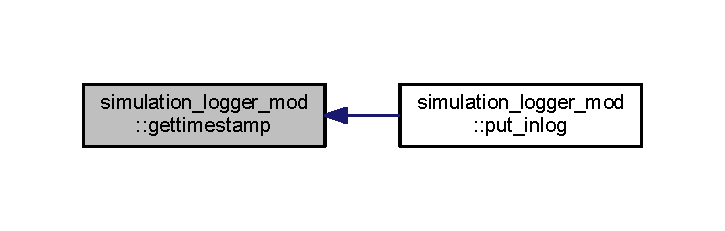
\includegraphics[width=348pt]{namespacesimulation__logger__mod_a0326a5eeb649b041064a01d96aef0989_icgraph}
\end{center}
\end{figure}
\mbox{\Hypertarget{namespacesimulation__logger__mod_abf603e657da9104a8060ab53c72f0aca}\label{namespacesimulation__logger__mod_abf603e657da9104a8060ab53c72f0aca}} 
\index{simulation\+\_\+logger\+\_\+mod@{simulation\+\_\+logger\+\_\+mod}!initlog@{initlog}}
\index{initlog@{initlog}!simulation\+\_\+logger\+\_\+mod@{simulation\+\_\+logger\+\_\+mod}}
\subsubsection{\texorpdfstring{initlog()}{initlog()}}
{\footnotesize\ttfamily subroutine simulation\+\_\+logger\+\_\+mod\+::initlog (\begin{DoxyParamCaption}\item[{class(\hyperlink{structsimulation__logger__mod_1_1logger__class}{logger\+\_\+class}), intent(inout)}]{self,  }\item[{type(string), intent(in)}]{outpath }\end{DoxyParamCaption})\hspace{0.3cm}{\ttfamily [private]}}



Log file initizalization routine. 

\begin{DoxyAuthor}{Author}
Ricardo Birjukovs Canelas -\/ M\+A\+R\+E\+T\+EC 
\end{DoxyAuthor}

\begin{DoxyParams}[1]{Parameters}
\mbox{\tt in}  & {\em outpath} & \\
\hline
\mbox{\tt in}  & {\em outpath} & output path were to point the logger \\
\hline
\end{DoxyParams}
\mbox{\Hypertarget{namespacesimulation__logger__mod_a34980631cfcf2d2172aa3b491acace4c}\label{namespacesimulation__logger__mod_a34980631cfcf2d2172aa3b491acace4c}} 
\index{simulation\+\_\+logger\+\_\+mod@{simulation\+\_\+logger\+\_\+mod}!put\+\_\+inlog@{put\+\_\+inlog}}
\index{put\+\_\+inlog@{put\+\_\+inlog}!simulation\+\_\+logger\+\_\+mod@{simulation\+\_\+logger\+\_\+mod}}
\subsubsection{\texorpdfstring{put\+\_\+inlog()}{put\_inlog()}}
{\footnotesize\ttfamily subroutine simulation\+\_\+logger\+\_\+mod\+::put\+\_\+inlog (\begin{DoxyParamCaption}\item[{class(\hyperlink{structsimulation__logger__mod_1_1logger__class}{logger\+\_\+class}), intent(in)}]{self,  }\item[{type(string), intent(inout)}]{tologstr,  }\item[{logical, intent(in), optional}]{timeoption }\end{DoxyParamCaption})\hspace{0.3cm}{\ttfamily [private]}}



Log serialization routine. 

\begin{DoxyAuthor}{Author}
Ricardo Birjukovs Canelas -\/ M\+A\+R\+E\+T\+EC 
\end{DoxyAuthor}

\begin{DoxyParams}[1]{Parameters}
\mbox{\tt in}  & {\em tologstr,timeoption} & \\
\hline
\end{DoxyParams}
Here is the call graph for this function\+:\nopagebreak
\begin{figure}[H]
\begin{center}
\leavevmode
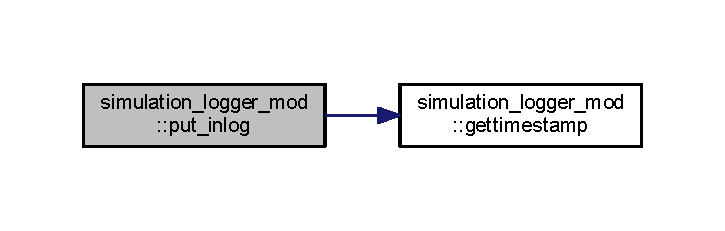
\includegraphics[width=348pt]{namespacesimulation__logger__mod_a34980631cfcf2d2172aa3b491acace4c_cgraph}
\end{center}
\end{figure}


\subsection{Variable Documentation}
\mbox{\Hypertarget{namespacesimulation__logger__mod_aa778de9905350741e1f40bb04fdc1cf6}\label{namespacesimulation__logger__mod_aa778de9905350741e1f40bb04fdc1cf6}} 
\index{simulation\+\_\+logger\+\_\+mod@{simulation\+\_\+logger\+\_\+mod}!log@{log}}
\index{log@{log}!simulation\+\_\+logger\+\_\+mod@{simulation\+\_\+logger\+\_\+mod}}
\subsubsection{\texorpdfstring{log}{log}}
{\footnotesize\ttfamily type(\hyperlink{structsimulation__logger__mod_1_1logger__class}{logger\+\_\+class}), public simulation\+\_\+logger\+\_\+mod\+::log}


\hypertarget{namespacesimulation__memory__mod}{}\section{simulation\+\_\+memory\+\_\+mod Module Reference}
\label{namespacesimulation__memory__mod}\index{simulation\+\_\+memory\+\_\+mod@{simulation\+\_\+memory\+\_\+mod}}


Module to hold the simulation memory managment class and its methods.  


\subsection*{Data Types}
\begin{DoxyCompactItemize}
\item 
type \hyperlink{structsimulation__memory__mod_1_1memory__t}{memory\+\_\+t}
\end{DoxyCompactItemize}
\subsection*{Functions/\+Subroutines}
\begin{DoxyCompactItemize}
\item 
subroutine \hyperlink{namespacesimulation__memory__mod_ac8306165e4ec88fec9a2b8b719f61893}{initializememory} (self)
\begin{DoxyCompactList}\small\item\em Birjukovs Canelas -\/ M\+A\+R\+E\+T\+EC \end{DoxyCompactList}\item 
subroutine \hyperlink{namespacesimulation__memory__mod_acf04d6b930ed3ffbc0950afd86033c51}{getotal} (self, size)
\begin{DoxyCompactList}\small\item\em Birjukovs Canelas -\/ M\+A\+R\+E\+T\+EC \end{DoxyCompactList}\item 
subroutine \hyperlink{namespacesimulation__memory__mod_a4169689db37b3ba35e092096a7019f80}{addblock} (self, size)
\begin{DoxyCompactList}\small\item\em Birjukovs Canelas -\/ M\+A\+R\+E\+T\+EC \end{DoxyCompactList}\item 
subroutine \hyperlink{namespacesimulation__memory__mod_a940ff42fa3a49423f9ac98da2bffa54c}{addsource} (self, size)
\begin{DoxyCompactList}\small\item\em Birjukovs Canelas -\/ M\+A\+R\+E\+T\+EC \end{DoxyCompactList}\item 
subroutine \hyperlink{namespacesimulation__memory__mod_a5770021491589bbd61ea112d113a9c9d}{addtracer} (self, size)
\begin{DoxyCompactList}\small\item\em Birjukovs Canelas -\/ M\+A\+R\+E\+T\+EC \end{DoxyCompactList}\item 
subroutine \hyperlink{namespacesimulation__memory__mod_a5f95539e9740401e7046b79c40ad2ecd}{removetracer} (self, size)
\begin{DoxyCompactList}\small\item\em Birjukovs Canelas -\/ M\+A\+R\+E\+T\+EC \end{DoxyCompactList}\item 
subroutine \hyperlink{namespacesimulation__memory__mod_ac6d6853bc462947d24a8f6234d625138}{adddef} (self, size)
\begin{DoxyCompactList}\small\item\em Birjukovs Canelas -\/ M\+A\+R\+E\+T\+EC \end{DoxyCompactList}\item 
subroutine \hyperlink{namespacesimulation__memory__mod_a16a7a1c7e88fe5a5523d23f83f0e04a0}{printmemory} (self)
\begin{DoxyCompactList}\small\item\em Birjukovs Canelas -\/ M\+A\+R\+E\+T\+EC \end{DoxyCompactList}\item 
subroutine \hyperlink{namespacesimulation__memory__mod_a894bd4ec7462fd634d328ee5be4c6483}{printmemorydetailed} (self)
\begin{DoxyCompactList}\small\item\em Birjukovs Canelas -\/ M\+A\+R\+E\+T\+EC \end{DoxyCompactList}\end{DoxyCompactItemize}
\subsection*{Variables}
\begin{DoxyCompactItemize}
\item 
type(\hyperlink{structsimulation__memory__mod_1_1memory__t}{memory\+\_\+t}), public \hyperlink{namespacesimulation__memory__mod_af3e2714796469b4b1ec247569b184088}{simmemory}
\end{DoxyCompactItemize}


\subsection{Detailed Description}
Module to hold the simulation memory managment class and its methods. 

\begin{DoxyAuthor}{Author}
Ricardo Birjukovs Canelas 
\end{DoxyAuthor}


\subsection{Function/\+Subroutine Documentation}
\mbox{\Hypertarget{namespacesimulation__memory__mod_a4169689db37b3ba35e092096a7019f80}\label{namespacesimulation__memory__mod_a4169689db37b3ba35e092096a7019f80}} 
\index{simulation\+\_\+memory\+\_\+mod@{simulation\+\_\+memory\+\_\+mod}!addblock@{addblock}}
\index{addblock@{addblock}!simulation\+\_\+memory\+\_\+mod@{simulation\+\_\+memory\+\_\+mod}}
\subsubsection{\texorpdfstring{addblock()}{addblock()}}
{\footnotesize\ttfamily subroutine simulation\+\_\+memory\+\_\+mod\+::addblock (\begin{DoxyParamCaption}\item[{class(\hyperlink{structsimulation__memory__mod_1_1memory__t}{memory\+\_\+t}), intent(inout)}]{self,  }\item[{integer, intent(in)}]{size }\end{DoxyParamCaption})\hspace{0.3cm}{\ttfamily [private]}}



Birjukovs Canelas -\/ M\+A\+R\+E\+T\+EC 

Private method to add the size of a Block to the memory log. \mbox{\Hypertarget{namespacesimulation__memory__mod_ac6d6853bc462947d24a8f6234d625138}\label{namespacesimulation__memory__mod_ac6d6853bc462947d24a8f6234d625138}} 
\index{simulation\+\_\+memory\+\_\+mod@{simulation\+\_\+memory\+\_\+mod}!adddef@{adddef}}
\index{adddef@{adddef}!simulation\+\_\+memory\+\_\+mod@{simulation\+\_\+memory\+\_\+mod}}
\subsubsection{\texorpdfstring{adddef()}{adddef()}}
{\footnotesize\ttfamily subroutine simulation\+\_\+memory\+\_\+mod\+::adddef (\begin{DoxyParamCaption}\item[{class(\hyperlink{structsimulation__memory__mod_1_1memory__t}{memory\+\_\+t}), intent(inout)}]{self,  }\item[{integer, intent(in)}]{size }\end{DoxyParamCaption})\hspace{0.3cm}{\ttfamily [private]}}



Birjukovs Canelas -\/ M\+A\+R\+E\+T\+EC 

Private method to add the size of a definition to the memory log. \mbox{\Hypertarget{namespacesimulation__memory__mod_a940ff42fa3a49423f9ac98da2bffa54c}\label{namespacesimulation__memory__mod_a940ff42fa3a49423f9ac98da2bffa54c}} 
\index{simulation\+\_\+memory\+\_\+mod@{simulation\+\_\+memory\+\_\+mod}!addsource@{addsource}}
\index{addsource@{addsource}!simulation\+\_\+memory\+\_\+mod@{simulation\+\_\+memory\+\_\+mod}}
\subsubsection{\texorpdfstring{addsource()}{addsource()}}
{\footnotesize\ttfamily subroutine simulation\+\_\+memory\+\_\+mod\+::addsource (\begin{DoxyParamCaption}\item[{class(\hyperlink{structsimulation__memory__mod_1_1memory__t}{memory\+\_\+t}), intent(inout)}]{self,  }\item[{integer, intent(in)}]{size }\end{DoxyParamCaption})\hspace{0.3cm}{\ttfamily [private]}}



Birjukovs Canelas -\/ M\+A\+R\+E\+T\+EC 

Private method to add the size of a Source to the memory log. \mbox{\Hypertarget{namespacesimulation__memory__mod_a5770021491589bbd61ea112d113a9c9d}\label{namespacesimulation__memory__mod_a5770021491589bbd61ea112d113a9c9d}} 
\index{simulation\+\_\+memory\+\_\+mod@{simulation\+\_\+memory\+\_\+mod}!addtracer@{addtracer}}
\index{addtracer@{addtracer}!simulation\+\_\+memory\+\_\+mod@{simulation\+\_\+memory\+\_\+mod}}
\subsubsection{\texorpdfstring{addtracer()}{addtracer()}}
{\footnotesize\ttfamily subroutine simulation\+\_\+memory\+\_\+mod\+::addtracer (\begin{DoxyParamCaption}\item[{class(\hyperlink{structsimulation__memory__mod_1_1memory__t}{memory\+\_\+t}), intent(inout)}]{self,  }\item[{integer, intent(in)}]{size }\end{DoxyParamCaption})\hspace{0.3cm}{\ttfamily [private]}}



Birjukovs Canelas -\/ M\+A\+R\+E\+T\+EC 

Private method to add the size of a Tracer to the memory log. \mbox{\Hypertarget{namespacesimulation__memory__mod_acf04d6b930ed3ffbc0950afd86033c51}\label{namespacesimulation__memory__mod_acf04d6b930ed3ffbc0950afd86033c51}} 
\index{simulation\+\_\+memory\+\_\+mod@{simulation\+\_\+memory\+\_\+mod}!getotal@{getotal}}
\index{getotal@{getotal}!simulation\+\_\+memory\+\_\+mod@{simulation\+\_\+memory\+\_\+mod}}
\subsubsection{\texorpdfstring{getotal()}{getotal()}}
{\footnotesize\ttfamily subroutine simulation\+\_\+memory\+\_\+mod\+::getotal (\begin{DoxyParamCaption}\item[{class(\hyperlink{structsimulation__memory__mod_1_1memory__t}{memory\+\_\+t}), intent(inout)}]{self,  }\item[{integer, intent(out)}]{size }\end{DoxyParamCaption})\hspace{0.3cm}{\ttfamily [private]}}



Birjukovs Canelas -\/ M\+A\+R\+E\+T\+EC 

Private method to retreive the total size of the allocated memory. \mbox{\Hypertarget{namespacesimulation__memory__mod_ac8306165e4ec88fec9a2b8b719f61893}\label{namespacesimulation__memory__mod_ac8306165e4ec88fec9a2b8b719f61893}} 
\index{simulation\+\_\+memory\+\_\+mod@{simulation\+\_\+memory\+\_\+mod}!initializememory@{initializememory}}
\index{initializememory@{initializememory}!simulation\+\_\+memory\+\_\+mod@{simulation\+\_\+memory\+\_\+mod}}
\subsubsection{\texorpdfstring{initializememory()}{initializememory()}}
{\footnotesize\ttfamily subroutine simulation\+\_\+memory\+\_\+mod\+::initializememory (\begin{DoxyParamCaption}\item[{class(\hyperlink{structsimulation__memory__mod_1_1memory__t}{memory\+\_\+t}), intent(inout)}]{self }\end{DoxyParamCaption})\hspace{0.3cm}{\ttfamily [private]}}



Birjukovs Canelas -\/ M\+A\+R\+E\+T\+EC 

Private memory logger initialization method. \mbox{\Hypertarget{namespacesimulation__memory__mod_a16a7a1c7e88fe5a5523d23f83f0e04a0}\label{namespacesimulation__memory__mod_a16a7a1c7e88fe5a5523d23f83f0e04a0}} 
\index{simulation\+\_\+memory\+\_\+mod@{simulation\+\_\+memory\+\_\+mod}!printmemory@{printmemory}}
\index{printmemory@{printmemory}!simulation\+\_\+memory\+\_\+mod@{simulation\+\_\+memory\+\_\+mod}}
\subsubsection{\texorpdfstring{printmemory()}{printmemory()}}
{\footnotesize\ttfamily subroutine simulation\+\_\+memory\+\_\+mod\+::printmemory (\begin{DoxyParamCaption}\item[{class(\hyperlink{structsimulation__memory__mod_1_1memory__t}{memory\+\_\+t}), intent(inout)}]{self }\end{DoxyParamCaption})\hspace{0.3cm}{\ttfamily [private]}}



Birjukovs Canelas -\/ M\+A\+R\+E\+T\+EC 

Method to print the total allocated memory. \mbox{\Hypertarget{namespacesimulation__memory__mod_a894bd4ec7462fd634d328ee5be4c6483}\label{namespacesimulation__memory__mod_a894bd4ec7462fd634d328ee5be4c6483}} 
\index{simulation\+\_\+memory\+\_\+mod@{simulation\+\_\+memory\+\_\+mod}!printmemorydetailed@{printmemorydetailed}}
\index{printmemorydetailed@{printmemorydetailed}!simulation\+\_\+memory\+\_\+mod@{simulation\+\_\+memory\+\_\+mod}}
\subsubsection{\texorpdfstring{printmemorydetailed()}{printmemorydetailed()}}
{\footnotesize\ttfamily subroutine simulation\+\_\+memory\+\_\+mod\+::printmemorydetailed (\begin{DoxyParamCaption}\item[{class(\hyperlink{structsimulation__memory__mod_1_1memory__t}{memory\+\_\+t}), intent(inout)}]{self }\end{DoxyParamCaption})\hspace{0.3cm}{\ttfamily [private]}}



Birjukovs Canelas -\/ M\+A\+R\+E\+T\+EC 

Private method to print the allocated memory. \mbox{\Hypertarget{namespacesimulation__memory__mod_a5f95539e9740401e7046b79c40ad2ecd}\label{namespacesimulation__memory__mod_a5f95539e9740401e7046b79c40ad2ecd}} 
\index{simulation\+\_\+memory\+\_\+mod@{simulation\+\_\+memory\+\_\+mod}!removetracer@{removetracer}}
\index{removetracer@{removetracer}!simulation\+\_\+memory\+\_\+mod@{simulation\+\_\+memory\+\_\+mod}}
\subsubsection{\texorpdfstring{removetracer()}{removetracer()}}
{\footnotesize\ttfamily subroutine simulation\+\_\+memory\+\_\+mod\+::removetracer (\begin{DoxyParamCaption}\item[{class(\hyperlink{structsimulation__memory__mod_1_1memory__t}{memory\+\_\+t}), intent(inout)}]{self,  }\item[{integer, intent(in)}]{size }\end{DoxyParamCaption})\hspace{0.3cm}{\ttfamily [private]}}



Birjukovs Canelas -\/ M\+A\+R\+E\+T\+EC 

Private method to remove the size of a Tracer from the memory log. 

\subsection{Variable Documentation}
\mbox{\Hypertarget{namespacesimulation__memory__mod_af3e2714796469b4b1ec247569b184088}\label{namespacesimulation__memory__mod_af3e2714796469b4b1ec247569b184088}} 
\index{simulation\+\_\+memory\+\_\+mod@{simulation\+\_\+memory\+\_\+mod}!simmemory@{simmemory}}
\index{simmemory@{simmemory}!simulation\+\_\+memory\+\_\+mod@{simulation\+\_\+memory\+\_\+mod}}
\subsubsection{\texorpdfstring{simmemory}{simmemory}}
{\footnotesize\ttfamily type(\hyperlink{structsimulation__memory__mod_1_1memory__t}{memory\+\_\+t}), public simulation\+\_\+memory\+\_\+mod\+::simmemory}


\hypertarget{namespacesimulation__mod}{}\section{simulation\+\_\+mod Module Reference}
\label{namespacesimulation__mod}\index{simulation\+\_\+mod@{simulation\+\_\+mod}}


Module to hold the simulation class and its methods. This is the only class that is exposed to an external program, as it encapsulates every other class and method.  


\subsection*{Data Types}
\begin{DoxyCompactItemize}
\item 
type \mbox{\hyperlink{structsimulation__mod_1_1simulation__class}{simulation\+\_\+class}}
\end{DoxyCompactItemize}
\subsection*{Functions/\+Subroutines}
\begin{DoxyCompactItemize}
\item 
subroutine \mbox{\hyperlink{namespacesimulation__mod_a73bd78c4ac76c51f1e10f5847c25c4df}{run}} (self)
\begin{DoxyCompactList}\small\item\em Simulation run method. Runs the initialized case main time cycle. \end{DoxyCompactList}\item 
subroutine \mbox{\hyperlink{namespacesimulation__mod_aedbba2bb458cbcd7eb93938a5f7b5940}{initsimulation}} (self, casefilename, outpath)
\begin{DoxyCompactList}\small\item\em Simulation initialization method. Effectively builds and populates the simulation objects that will be used latter on. \end{DoxyCompactList}\item 
subroutine \mbox{\hyperlink{namespacesimulation__mod_a87a5141e4516b9610a6e4f0d2ff2d719}{togglesources}} (self)
\begin{DoxyCompactList}\small\item\em Simulation method to activate and deactivate Sources based on the GlobalSim\+Time. \end{DoxyCompactList}\item 
subroutine \mbox{\hyperlink{namespacesimulation__mod_a13aa0745f4601e3f418143dab2f18276}{blocksemitt}} (self)
\begin{DoxyCompactList}\small\item\em Simulation method to call the Blocks to emitt tracers at current Sim\+Time. \end{DoxyCompactList}\item 
subroutine \mbox{\hyperlink{namespacesimulation__mod_a058892630af07fc0fe8a4bffec531c6a}{blocksdistribute}} (self)
\begin{DoxyCompactList}\small\item\em Simulation method to call the Blocks to distribute Tracers at current Sim\+Time. \end{DoxyCompactList}\item 
subroutine \mbox{\hyperlink{namespacesimulation__mod_ac838d4afe33303dc49a5790ca957baa1}{blocksconsolidatearrays}} (self)
\begin{DoxyCompactList}\small\item\em Simulation method to call the Blocks to consolidate the Tracer array at current Sim\+Time. \end{DoxyCompactList}\item 
subroutine \mbox{\hyperlink{namespacesimulation__mod_a624d5b402a8d359219839841862ab307}{blockstracerstoaot}} (self)
\begin{DoxyCompactList}\small\item\em Simulation method to call the Blocks to build their Array of Tracers (AoT) from the Tracer list at current Sim\+Time. \end{DoxyCompactList}\item 
subroutine \mbox{\hyperlink{namespacesimulation__mod_a03afd8682d3239c0ce8eb1637e4da806}{blocksaottotracers}} (self)
\begin{DoxyCompactList}\small\item\em Simulation method to call the Blocks to print their Array of Tracers (AoT) back to the Tracer objects on the list at current Sim\+Time. \end{DoxyCompactList}\item 
subroutine \mbox{\hyperlink{namespacesimulation__mod_a9c7e093e5cf65d3414f9a8cf8beab611}{blockscleanaot}} (self)
\begin{DoxyCompactList}\small\item\em Simulation method to call the Blocks to clean their Array of Tracers (AoT) at current Sim\+Time. \end{DoxyCompactList}\item 
subroutine \mbox{\hyperlink{namespacesimulation__mod_a447c6d709de6aa360a65d39d660e627b}{setinitialstate}} (self)
\begin{DoxyCompactList}\small\item\em Simulation method to distribute the Sources to the Blocks, allocate the respective Tracers and redistribute if needed. \end{DoxyCompactList}\item 
integer function \mbox{\hyperlink{namespacesimulation__mod_a0ad485eab624ffa4df282f1da8d9f214}{gettracertotals}} (self)
\begin{DoxyCompactList}\small\item\em Simulation method to count Tracer numbers. \end{DoxyCompactList}\item 
subroutine \mbox{\hyperlink{namespacesimulation__mod_aba126a8e0575cabb3bef6ab395002b3c}{printtracertotals}} (self)
\begin{DoxyCompactList}\small\item\em Simulation method to count Tracer numbers. \end{DoxyCompactList}\item 
subroutine \mbox{\hyperlink{namespacesimulation__mod_acc5fa823c8dd599de8feda8988c224f2}{settracermemory}} (self, ntrc)
\begin{DoxyCompactList}\small\item\em Simulation method to account for Tracer memory consumption. \end{DoxyCompactList}\item 
subroutine \mbox{\hyperlink{namespacesimulation__mod_a2b8198a9fb3f7671c6b45192a0b9740c}{decomposedomain}} (self)
\begin{DoxyCompactList}\small\item\em Simulation method to do domain decomposition and define the Blocks. \end{DoxyCompactList}\item 
subroutine \mbox{\hyperlink{namespacesimulation__mod_a4285722eaa589fa671233554b54c74f8}{closesimulation}} (self)
\begin{DoxyCompactList}\small\item\em Simulation finishing method. Closes output files and writes the final messages. \end{DoxyCompactList}\end{DoxyCompactItemize}


\subsection{Detailed Description}
Module to hold the simulation class and its methods. This is the only class that is exposed to an external program, as it encapsulates every other class and method. 

\begin{DoxyAuthor}{Author}
Ricardo Birjukovs Canelas 
\end{DoxyAuthor}


\subsection{Function/\+Subroutine Documentation}
\mbox{\Hypertarget{namespacesimulation__mod_a03afd8682d3239c0ce8eb1637e4da806}\label{namespacesimulation__mod_a03afd8682d3239c0ce8eb1637e4da806}} 
\index{simulation\+\_\+mod@{simulation\+\_\+mod}!blocksaottotracers@{blocksaottotracers}}
\index{blocksaottotracers@{blocksaottotracers}!simulation\+\_\+mod@{simulation\+\_\+mod}}
\subsubsection{\texorpdfstring{blocksaottotracers()}{blocksaottotracers()}}
{\footnotesize\ttfamily subroutine simulation\+\_\+mod\+::blocksaottotracers (\begin{DoxyParamCaption}\item[{class(\mbox{\hyperlink{structsimulation__mod_1_1simulation__class}{simulation\+\_\+class}}), intent(in)}]{self }\end{DoxyParamCaption})\hspace{0.3cm}{\ttfamily [private]}}



Simulation method to call the Blocks to print their Array of Tracers (AoT) back to the Tracer objects on the list at current Sim\+Time. 

\begin{DoxyAuthor}{Author}
Ricardo Birjukovs Canelas -\/ M\+A\+R\+E\+T\+EC 
\end{DoxyAuthor}


Definition at line 251 of file simulation.\+f90.


\begin{DoxyCode}
251     \textcolor{keywordtype}{implicit none}
252     \textcolor{keywordtype}{class}(simulation\_class), \textcolor{keywordtype}{intent(in)} :: self
253     \textcolor{keywordtype}{integer} :: i
254     \textcolor{keywordflow}{do} i=1, \textcolor{keyword}{size}(dblock)
255         \textcolor{keyword}{call }dblock(i)%AoTtoTracers()
256 \textcolor{keywordflow}{    enddo}
\end{DoxyCode}
\mbox{\Hypertarget{namespacesimulation__mod_a9c7e093e5cf65d3414f9a8cf8beab611}\label{namespacesimulation__mod_a9c7e093e5cf65d3414f9a8cf8beab611}} 
\index{simulation\+\_\+mod@{simulation\+\_\+mod}!blockscleanaot@{blockscleanaot}}
\index{blockscleanaot@{blockscleanaot}!simulation\+\_\+mod@{simulation\+\_\+mod}}
\subsubsection{\texorpdfstring{blockscleanaot()}{blockscleanaot()}}
{\footnotesize\ttfamily subroutine simulation\+\_\+mod\+::blockscleanaot (\begin{DoxyParamCaption}\item[{class(\mbox{\hyperlink{structsimulation__mod_1_1simulation__class}{simulation\+\_\+class}}), intent(in)}]{self }\end{DoxyParamCaption})\hspace{0.3cm}{\ttfamily [private]}}



Simulation method to call the Blocks to clean their Array of Tracers (AoT) at current Sim\+Time. 

\begin{DoxyAuthor}{Author}
Ricardo Birjukovs Canelas -\/ M\+A\+R\+E\+T\+EC 
\end{DoxyAuthor}


Definition at line 266 of file simulation.\+f90.


\begin{DoxyCode}
266     \textcolor{keywordtype}{implicit none}
267     \textcolor{keywordtype}{class}(simulation\_class), \textcolor{keywordtype}{intent(in)} :: self
268     \textcolor{keywordtype}{integer} :: i
269     \textcolor{keywordflow}{do} i=1, \textcolor{keyword}{size}(dblock)
270         \textcolor{keyword}{call }dblock(i)%CleanAoT()
271 \textcolor{keywordflow}{    enddo}
\end{DoxyCode}
\mbox{\Hypertarget{namespacesimulation__mod_ac838d4afe33303dc49a5790ca957baa1}\label{namespacesimulation__mod_ac838d4afe33303dc49a5790ca957baa1}} 
\index{simulation\+\_\+mod@{simulation\+\_\+mod}!blocksconsolidatearrays@{blocksconsolidatearrays}}
\index{blocksconsolidatearrays@{blocksconsolidatearrays}!simulation\+\_\+mod@{simulation\+\_\+mod}}
\subsubsection{\texorpdfstring{blocksconsolidatearrays()}{blocksconsolidatearrays()}}
{\footnotesize\ttfamily subroutine simulation\+\_\+mod\+::blocksconsolidatearrays (\begin{DoxyParamCaption}\item[{class(\mbox{\hyperlink{structsimulation__mod_1_1simulation__class}{simulation\+\_\+class}}), intent(in)}]{self }\end{DoxyParamCaption})\hspace{0.3cm}{\ttfamily [private]}}



Simulation method to call the Blocks to consolidate the Tracer array at current Sim\+Time. 

\begin{DoxyAuthor}{Author}
Ricardo Birjukovs Canelas -\/ M\+A\+R\+E\+T\+EC 
\end{DoxyAuthor}


Definition at line 221 of file simulation.\+f90.


\begin{DoxyCode}
221     \textcolor{keywordtype}{implicit none}
222     \textcolor{keywordtype}{class}(simulation\_class), \textcolor{keywordtype}{intent(in)} :: self
223     \textcolor{keywordtype}{integer} :: i
224     \textcolor{keywordflow}{do} i=1, \textcolor{keyword}{size}(dblock)
225         \textcolor{keyword}{call }dblock(i)%ConsolidateArrays()
226 \textcolor{keywordflow}{    enddo}
\end{DoxyCode}
\mbox{\Hypertarget{namespacesimulation__mod_a058892630af07fc0fe8a4bffec531c6a}\label{namespacesimulation__mod_a058892630af07fc0fe8a4bffec531c6a}} 
\index{simulation\+\_\+mod@{simulation\+\_\+mod}!blocksdistribute@{blocksdistribute}}
\index{blocksdistribute@{blocksdistribute}!simulation\+\_\+mod@{simulation\+\_\+mod}}
\subsubsection{\texorpdfstring{blocksdistribute()}{blocksdistribute()}}
{\footnotesize\ttfamily subroutine simulation\+\_\+mod\+::blocksdistribute (\begin{DoxyParamCaption}\item[{class(\mbox{\hyperlink{structsimulation__mod_1_1simulation__class}{simulation\+\_\+class}}), intent(in)}]{self }\end{DoxyParamCaption})\hspace{0.3cm}{\ttfamily [private]}}



Simulation method to call the Blocks to distribute Tracers at current Sim\+Time. 

\begin{DoxyAuthor}{Author}
Ricardo Birjukovs Canelas -\/ M\+A\+R\+E\+T\+EC 
\end{DoxyAuthor}


Definition at line 205 of file simulation.\+f90.


\begin{DoxyCode}
205     \textcolor{keywordtype}{implicit none}
206     \textcolor{keywordtype}{class}(simulation\_class), \textcolor{keywordtype}{intent(in)} :: self
207     \textcolor{keywordtype}{integer} :: i
208     \textcolor{keywordflow}{do} i=1, \textcolor{keyword}{size}(dblock)
209         \textcolor{keyword}{call }dblock(i)%DistributeTracers()
210 \textcolor{keywordflow}{    enddo}
211     \textcolor{comment}{!need to distribute Sources also! TODO}
\end{DoxyCode}
\mbox{\Hypertarget{namespacesimulation__mod_a13aa0745f4601e3f418143dab2f18276}\label{namespacesimulation__mod_a13aa0745f4601e3f418143dab2f18276}} 
\index{simulation\+\_\+mod@{simulation\+\_\+mod}!blocksemitt@{blocksemitt}}
\index{blocksemitt@{blocksemitt}!simulation\+\_\+mod@{simulation\+\_\+mod}}
\subsubsection{\texorpdfstring{blocksemitt()}{blocksemitt()}}
{\footnotesize\ttfamily subroutine simulation\+\_\+mod\+::blocksemitt (\begin{DoxyParamCaption}\item[{class(\mbox{\hyperlink{structsimulation__mod_1_1simulation__class}{simulation\+\_\+class}}), intent(in)}]{self }\end{DoxyParamCaption})\hspace{0.3cm}{\ttfamily [private]}}



Simulation method to call the Blocks to emitt tracers at current Sim\+Time. 

\begin{DoxyAuthor}{Author}
Ricardo Birjukovs Canelas -\/ M\+A\+R\+E\+T\+EC 
\end{DoxyAuthor}


Definition at line 190 of file simulation.\+f90.


\begin{DoxyCode}
190     \textcolor{keywordtype}{implicit none}
191     \textcolor{keywordtype}{class}(simulation\_class), \textcolor{keywordtype}{intent(in)} :: self
192     \textcolor{keywordtype}{integer} :: i
193     \textcolor{keywordflow}{do} i=1, \textcolor{keyword}{size}(dblock)
194         \textcolor{keyword}{call }dblock(i)%CallEmitter()
195 \textcolor{keywordflow}{    enddo}
\end{DoxyCode}
\mbox{\Hypertarget{namespacesimulation__mod_a624d5b402a8d359219839841862ab307}\label{namespacesimulation__mod_a624d5b402a8d359219839841862ab307}} 
\index{simulation\+\_\+mod@{simulation\+\_\+mod}!blockstracerstoaot@{blockstracerstoaot}}
\index{blockstracerstoaot@{blockstracerstoaot}!simulation\+\_\+mod@{simulation\+\_\+mod}}
\subsubsection{\texorpdfstring{blockstracerstoaot()}{blockstracerstoaot()}}
{\footnotesize\ttfamily subroutine simulation\+\_\+mod\+::blockstracerstoaot (\begin{DoxyParamCaption}\item[{class(\mbox{\hyperlink{structsimulation__mod_1_1simulation__class}{simulation\+\_\+class}}), intent(in)}]{self }\end{DoxyParamCaption})\hspace{0.3cm}{\ttfamily [private]}}



Simulation method to call the Blocks to build their Array of Tracers (AoT) from the Tracer list at current Sim\+Time. 

\begin{DoxyAuthor}{Author}
Ricardo Birjukovs Canelas -\/ M\+A\+R\+E\+T\+EC 
\end{DoxyAuthor}


Definition at line 236 of file simulation.\+f90.


\begin{DoxyCode}
236     \textcolor{keywordtype}{implicit none}
237     \textcolor{keywordtype}{class}(simulation\_class), \textcolor{keywordtype}{intent(in)} :: self
238     \textcolor{keywordtype}{integer} :: i
239     \textcolor{keywordflow}{do} i=1, \textcolor{keyword}{size}(dblock)
240         \textcolor{keyword}{call }dblock(i)%TracersToAoT()
241 \textcolor{keywordflow}{    enddo}
\end{DoxyCode}
\mbox{\Hypertarget{namespacesimulation__mod_a4285722eaa589fa671233554b54c74f8}\label{namespacesimulation__mod_a4285722eaa589fa671233554b54c74f8}} 
\index{simulation\+\_\+mod@{simulation\+\_\+mod}!closesimulation@{closesimulation}}
\index{closesimulation@{closesimulation}!simulation\+\_\+mod@{simulation\+\_\+mod}}
\subsubsection{\texorpdfstring{closesimulation()}{closesimulation()}}
{\footnotesize\ttfamily subroutine simulation\+\_\+mod\+::closesimulation (\begin{DoxyParamCaption}\item[{class(\mbox{\hyperlink{structsimulation__mod_1_1simulation__class}{simulation\+\_\+class}}), intent(inout)}]{self }\end{DoxyParamCaption})\hspace{0.3cm}{\ttfamily [private]}}



Simulation finishing method. Closes output files and writes the final messages. 

\begin{DoxyAuthor}{Author}
Ricardo Birjukovs Canelas -\/ M\+A\+R\+E\+T\+EC 
\end{DoxyAuthor}


Definition at line 379 of file simulation.\+f90.


\begin{DoxyCode}
379     \textcolor{keywordtype}{implicit none}
380     \textcolor{keywordtype}{class}(simulation\_class), \textcolor{keywordtype}{intent(inout)} :: self
381     \textcolor{keywordtype}{type}(string) :: outext
382     outext=\textcolor{stringliteral}{'Simulation ended, freeing resources. See you next time'}
383     \textcolor{keyword}{call }log%put(outext)
384     \textcolor{keyword}{call }log%finalize()
\end{DoxyCode}
\mbox{\Hypertarget{namespacesimulation__mod_a2b8198a9fb3f7671c6b45192a0b9740c}\label{namespacesimulation__mod_a2b8198a9fb3f7671c6b45192a0b9740c}} 
\index{simulation\+\_\+mod@{simulation\+\_\+mod}!decomposedomain@{decomposedomain}}
\index{decomposedomain@{decomposedomain}!simulation\+\_\+mod@{simulation\+\_\+mod}}
\subsubsection{\texorpdfstring{decomposedomain()}{decomposedomain()}}
{\footnotesize\ttfamily subroutine simulation\+\_\+mod\+::decomposedomain (\begin{DoxyParamCaption}\item[{class(\mbox{\hyperlink{structsimulation__mod_1_1simulation__class}{simulation\+\_\+class}}), intent(inout)}]{self }\end{DoxyParamCaption})\hspace{0.3cm}{\ttfamily [private]}}



Simulation method to do domain decomposition and define the Blocks. 

\begin{DoxyAuthor}{Author}
Ricardo Birjukovs Canelas -\/ M\+A\+R\+E\+T\+EC 
\end{DoxyAuthor}


Definition at line 359 of file simulation.\+f90.


\begin{DoxyCode}
359     \textcolor{keywordtype}{implicit none}
360     \textcolor{keywordtype}{class}(simulation\_class), \textcolor{keywordtype}{intent(inout)} :: self
361     \textcolor{keywordtype}{type}(string) :: outext
362     \textcolor{keywordflow}{if} (globals%SimDefs%autoblocksize) \textcolor{keywordflow}{then}
363         \textcolor{keyword}{call }allocblocks(globals%SimDefs%numblocks)
364     \textcolor{keywordflow}{else}
365         outext=\textcolor{stringliteral}{'[DecomposeDomain]: Only automatic Block sizing at the moment, stoping'}
366         \textcolor{keyword}{call }log%put(outext)
367         stop
368 \textcolor{keywordflow}{    end if}
369     \textcolor{comment}{! Initializing the Blocks}
370     \textcolor{keyword}{call }setblocks(globals%SimDefs%autoblocksize,globals%SimDefs%numblocks,globals%SimDefs%numblocksx,
      globals%SimDefs%numblocksy)
\end{DoxyCode}
Here is the call graph for this function\+:\nopagebreak
\begin{figure}[H]
\begin{center}
\leavevmode
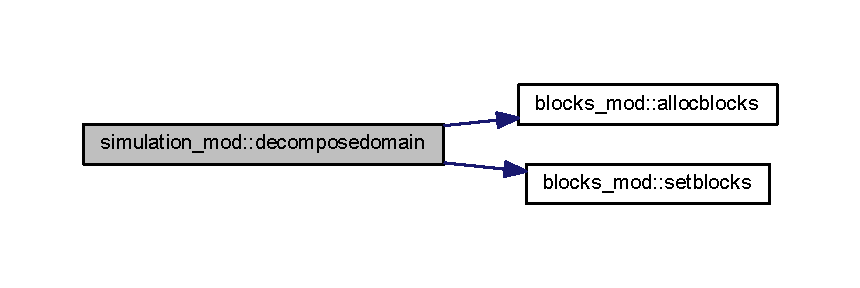
\includegraphics[width=350pt]{namespacesimulation__mod_a2b8198a9fb3f7671c6b45192a0b9740c_cgraph}
\end{center}
\end{figure}
\mbox{\Hypertarget{namespacesimulation__mod_a0ad485eab624ffa4df282f1da8d9f214}\label{namespacesimulation__mod_a0ad485eab624ffa4df282f1da8d9f214}} 
\index{simulation\+\_\+mod@{simulation\+\_\+mod}!gettracertotals@{gettracertotals}}
\index{gettracertotals@{gettracertotals}!simulation\+\_\+mod@{simulation\+\_\+mod}}
\subsubsection{\texorpdfstring{gettracertotals()}{gettracertotals()}}
{\footnotesize\ttfamily integer function simulation\+\_\+mod\+::gettracertotals (\begin{DoxyParamCaption}\item[{class(\mbox{\hyperlink{structsimulation__mod_1_1simulation__class}{simulation\+\_\+class}}), intent(in)}]{self }\end{DoxyParamCaption})\hspace{0.3cm}{\ttfamily [private]}}



Simulation method to count Tracer numbers. 

\begin{DoxyAuthor}{Author}
Ricardo Birjukovs Canelas -\/ M\+A\+R\+E\+T\+EC 
\end{DoxyAuthor}


Definition at line 307 of file simulation.\+f90.


\begin{DoxyCode}
307     \textcolor{keywordtype}{implicit none}
308     \textcolor{keywordtype}{class}(simulation\_class), \textcolor{keywordtype}{intent(in)} :: self
309     \textcolor{keywordtype}{integer} :: i, total
310     total = 0
311     \textcolor{keywordflow}{do} i=1, \textcolor{keyword}{size}(dblock)
312         total = total + dblock(i)%numAllocTracers()
313 \textcolor{keywordflow}{    enddo}
314     gettracertotals = total
\end{DoxyCode}
\mbox{\Hypertarget{namespacesimulation__mod_aedbba2bb458cbcd7eb93938a5f7b5940}\label{namespacesimulation__mod_aedbba2bb458cbcd7eb93938a5f7b5940}} 
\index{simulation\+\_\+mod@{simulation\+\_\+mod}!initsimulation@{initsimulation}}
\index{initsimulation@{initsimulation}!simulation\+\_\+mod@{simulation\+\_\+mod}}
\subsubsection{\texorpdfstring{initsimulation()}{initsimulation()}}
{\footnotesize\ttfamily subroutine simulation\+\_\+mod\+::initsimulation (\begin{DoxyParamCaption}\item[{class(\mbox{\hyperlink{structsimulation__mod_1_1simulation__class}{simulation\+\_\+class}}), intent(inout)}]{self,  }\item[{type(string), intent(in)}]{casefilename,  }\item[{type(string), intent(in)}]{outpath }\end{DoxyParamCaption})\hspace{0.3cm}{\ttfamily [private]}}



Simulation initialization method. Effectively builds and populates the simulation objects that will be used latter on. 

\begin{DoxyAuthor}{Author}
Ricardo Birjukovs Canelas -\/ M\+A\+R\+E\+T\+EC 
\end{DoxyAuthor}

\begin{DoxyParams}[1]{Parameters}
\mbox{\tt in}  & {\em self,casefilename,outpath} & \\
\hline
\mbox{\tt in}  & {\em casefilename} & case file name\\
\hline
\mbox{\tt in}  & {\em outpath} & Output path \\
\hline
\end{DoxyParams}


Definition at line 123 of file simulation.\+f90.


\begin{DoxyCode}
123     \textcolor{keywordtype}{implicit none}
124     \textcolor{keywordtype}{class}(simulation\_class), \textcolor{keywordtype}{intent(inout)} :: self
125     \textcolor{keywordtype}{type}(string), \textcolor{keywordtype}{intent(in)} :: casefilename
126     \textcolor{keywordtype}{type}(string), \textcolor{keywordtype}{intent(in)} :: outpath
127     \textcolor{keywordtype}{type}(string) :: outext
128     \textcolor{comment}{!type(generic\_field\_class) :: testField}
129     \textcolor{comment}{!type(background\_class) :: testBackground}
130 
131     \textcolor{comment}{! Initialize logger}
132     \textcolor{keyword}{call }log%initialize(outpath)
133     \textcolor{comment}{!Print licences and build info}
134     \textcolor{keyword}{call }printlicpreamble
135     \textcolor{comment}{!initializing memory log}
136     \textcolor{keyword}{call }simmemory%initialize()
137     \textcolor{comment}{!setting every global variable and input parameter to their default}
138     \textcolor{keyword}{call }globals%initialize(outpath = outpath)
139     \textcolor{comment}{!initializing geometry class}
140     \textcolor{keyword}{call }geometry%initialize()
141     \textcolor{comment}{!Check if case file has .xml extension}
142     \textcolor{keywordflow}{if} (casefilename%extension() == \textcolor{stringliteral}{'.xml'}) \textcolor{keywordflow}{then}
143         \textcolor{comment}{! Initialization routines to build the simulation from the input case file}
144         \textcolor{keyword}{call }initfromxml(casefilename)
145     \textcolor{keywordflow}{else}
146         outext=\textcolor{stringliteral}{'[initSimulation]: only .xml input files are supported at the time. Stopping'}
147         \textcolor{keyword}{call }log%put(outext)
148         stop
149 \textcolor{keywordflow}{    endif}
150     \textcolor{comment}{!Case was read and now we can build/initialize our simulation objects that are case-dependent}
151     \textcolor{comment}{!initilize simulation bounding box}
152     \textcolor{keyword}{call }bbox%initialize()
153     \textcolor{comment}{!decomposing the domain and initializing the Simulation Blocks}
154     \textcolor{keyword}{call }self%decompose()
155     \textcolor{comment}{!Distributing Sources}
156     \textcolor{keyword}{call }self%setInitialState()
157     \textcolor{comment}{!printing memory occupation at the time}
158     \textcolor{keyword}{call }simmemory%detailedprint()
159     \textcolor{comment}{!Initializing output file streamer}
160     \textcolor{keyword}{call }outputstreamer%initialize()
161     \textcolor{comment}{!Writing the domain to file}
162     \textcolor{keyword}{call }outputstreamer%WriteDomain(globals%Names%casename, bbox, geometry%getnumPoints(bbox), dblock)
163 
164     \textcolor{comment}{!call testField%test()}
165     \textcolor{comment}{!call testBackground%test()}
166 
\end{DoxyCode}
Here is the call graph for this function\+:\nopagebreak
\begin{figure}[H]
\begin{center}
\leavevmode
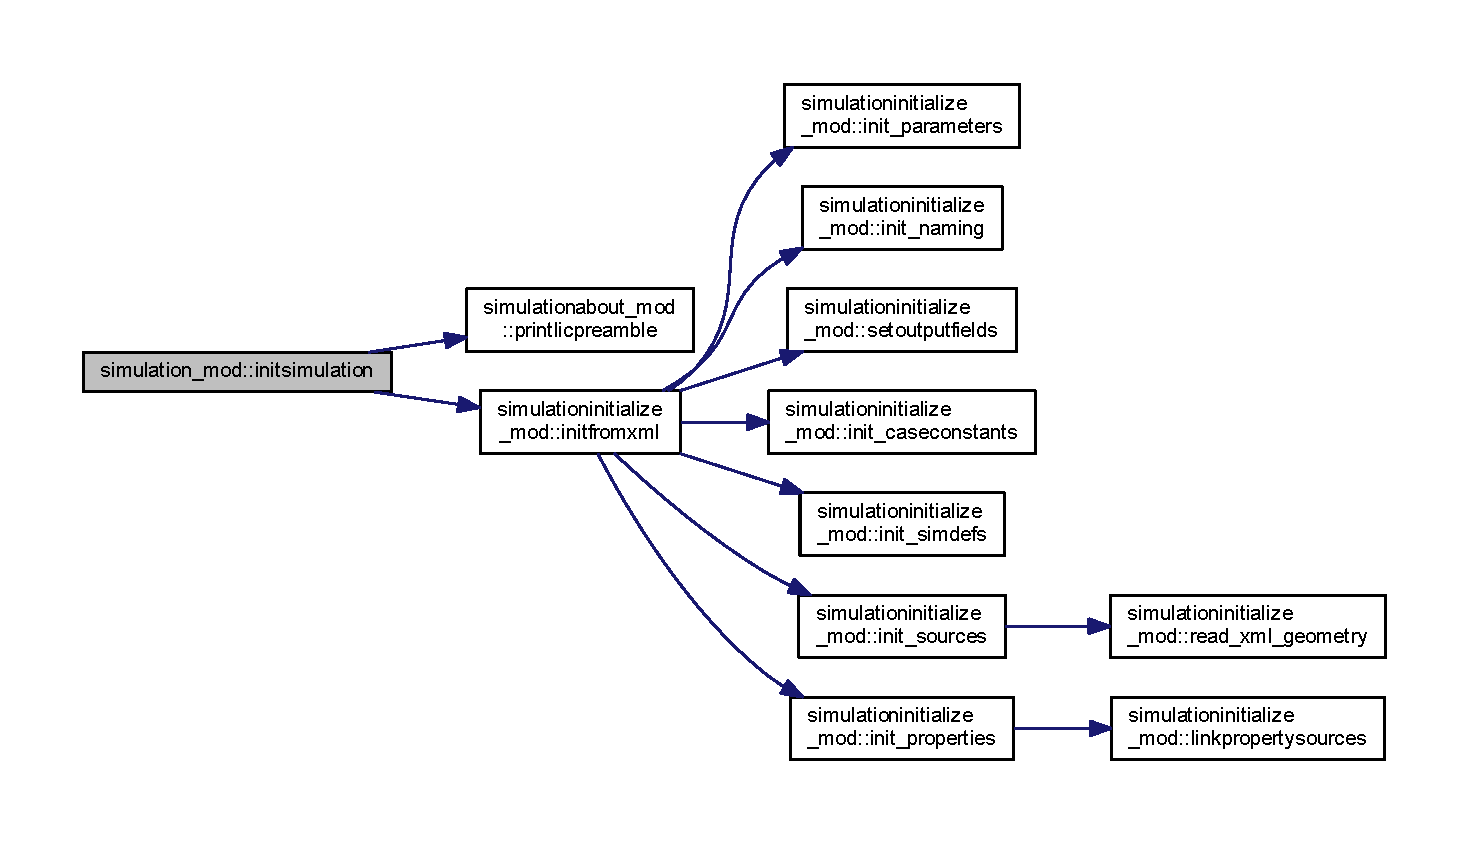
\includegraphics[width=350pt]{namespacesimulation__mod_aedbba2bb458cbcd7eb93938a5f7b5940_cgraph}
\end{center}
\end{figure}
\mbox{\Hypertarget{namespacesimulation__mod_aba126a8e0575cabb3bef6ab395002b3c}\label{namespacesimulation__mod_aba126a8e0575cabb3bef6ab395002b3c}} 
\index{simulation\+\_\+mod@{simulation\+\_\+mod}!printtracertotals@{printtracertotals}}
\index{printtracertotals@{printtracertotals}!simulation\+\_\+mod@{simulation\+\_\+mod}}
\subsubsection{\texorpdfstring{printtracertotals()}{printtracertotals()}}
{\footnotesize\ttfamily subroutine simulation\+\_\+mod\+::printtracertotals (\begin{DoxyParamCaption}\item[{class(\mbox{\hyperlink{structsimulation__mod_1_1simulation__class}{simulation\+\_\+class}}), intent(in)}]{self }\end{DoxyParamCaption})\hspace{0.3cm}{\ttfamily [private]}}



Simulation method to count Tracer numbers. 

\begin{DoxyAuthor}{Author}
Ricardo Birjukovs Canelas -\/ M\+A\+R\+E\+T\+EC 
\end{DoxyAuthor}


Definition at line 323 of file simulation.\+f90.


\begin{DoxyCode}
323     \textcolor{keywordtype}{implicit none}
324     \textcolor{keywordtype}{class}(simulation\_class), \textcolor{keywordtype}{intent(in)} :: self
325     \textcolor{keywordtype}{type}(string) :: outext, temp
326     temp = self%getTracerTotals()
327     outext=\textcolor{stringliteral}{'-->'}//temp //\textcolor{stringliteral}{' Tracers allocated'}
328     \textcolor{keyword}{call }log%put(outext,.false.)
\end{DoxyCode}
\mbox{\Hypertarget{namespacesimulation__mod_a73bd78c4ac76c51f1e10f5847c25c4df}\label{namespacesimulation__mod_a73bd78c4ac76c51f1e10f5847c25c4df}} 
\index{simulation\+\_\+mod@{simulation\+\_\+mod}!run@{run}}
\index{run@{run}!simulation\+\_\+mod@{simulation\+\_\+mod}}
\subsubsection{\texorpdfstring{run()}{run()}}
{\footnotesize\ttfamily subroutine simulation\+\_\+mod\+::run (\begin{DoxyParamCaption}\item[{class(\mbox{\hyperlink{structsimulation__mod_1_1simulation__class}{simulation\+\_\+class}}), intent(inout)}]{self }\end{DoxyParamCaption})\hspace{0.3cm}{\ttfamily [private]}}



Simulation run method. Runs the initialized case main time cycle. 

\begin{DoxyAuthor}{Author}
Ricardo Birjukovs Canelas -\/ M\+A\+R\+E\+T\+EC 
\end{DoxyAuthor}


Definition at line 68 of file simulation.\+f90.


\begin{DoxyCode}
68     \textcolor{keywordtype}{implicit none}
69     \textcolor{keywordtype}{class}(simulation\_class), \textcolor{keywordtype}{intent(inout)} :: self
70     \textcolor{keywordtype}{type}(string) :: outext
71 
72     outext = \textcolor{stringliteral}{'====================================================================='}
73     \textcolor{keyword}{call }log%put(outext,.false.)
74     outext = \textcolor{stringliteral}{'->Simulation starting'}
75     \textcolor{keyword}{call }log%put(outext)
76     outext = \textcolor{stringliteral}{'====================================================================='}
77     \textcolor{keyword}{call }log%put(outext,.false.)
78 
79     \textcolor{comment}{!main time cycle}
80     \textcolor{keywordflow}{do} \textcolor{keywordflow}{while} (globals%SimTime .lt. globals%Parameters%TimeMax)
81         \textcolor{comment}{!activate suitable Sources}
82         \textcolor{keyword}{call }self%ToggleSources()
83         \textcolor{comment}{!emitt Tracers from active Sources}
84         \textcolor{keyword}{call }self%BlocksEmitt()
85         \textcolor{comment}{!Distribute Tracers and Sources by Blocks}
86         \textcolor{keyword}{call }self%BlocksDistribute()
87         \textcolor{comment}{!Optimize Block Tracer lists}
88         \textcolor{keyword}{call }self%BlocksConsolidateArrays()
89         \textcolor{comment}{!Build AoT}
90         \textcolor{keyword}{call }self%BlocksTracersToAoT()
91         \textcolor{comment}{!load hydrodynamic fields from files (curents, wind, waves, ...)}
92         \textcolor{comment}{!Update all tracers with base behavior (AoT) - Integration step}
93         \textcolor{comment}{!interpolate fields to tracer coordinates}
94         \textcolor{comment}{!AoT to Tracers}
95         \textcolor{keyword}{call }self%BlocksAoTtoTracers()
96         \textcolor{comment}{!Update Tracers with type-specific behavior}
97         \textcolor{comment}{!Write results if time to do so}
98         \textcolor{keyword}{call }outputstreamer%WriteStepSerial(dblock)
99         \textcolor{comment}{!Print some stats from the time step}
100         \textcolor{keyword}{call }self%printTracerTotals()
101         \textcolor{comment}{!Clean AoT}
102         \textcolor{keyword}{call }self%BlocksCleanAoT()
103         \textcolor{comment}{!update Simulation time and counters}
104         globals%SimTime = globals%SimTime + globals%SimDefs%dt
105         \textcolor{keyword}{call }globals%Sim%increment\_numdt()
106         \textcolor{comment}{!print*, 'Global time is ', Globals%SimTime}
107         \textcolor{comment}{!print*, 'Can we continue?'}
108         \textcolor{comment}{!read (*,*)}
109 \textcolor{keywordflow}{    enddo}
110     \textcolor{keyword}{call }self%setTracerMemory()
111     \textcolor{keyword}{call }simmemory%detailedprint()
112 
\end{DoxyCode}
\mbox{\Hypertarget{namespacesimulation__mod_a447c6d709de6aa360a65d39d660e627b}\label{namespacesimulation__mod_a447c6d709de6aa360a65d39d660e627b}} 
\index{simulation\+\_\+mod@{simulation\+\_\+mod}!setinitialstate@{setinitialstate}}
\index{setinitialstate@{setinitialstate}!simulation\+\_\+mod@{simulation\+\_\+mod}}
\subsubsection{\texorpdfstring{setinitialstate()}{setinitialstate()}}
{\footnotesize\ttfamily subroutine simulation\+\_\+mod\+::setinitialstate (\begin{DoxyParamCaption}\item[{class(\mbox{\hyperlink{structsimulation__mod_1_1simulation__class}{simulation\+\_\+class}}), intent(inout)}]{self }\end{DoxyParamCaption})\hspace{0.3cm}{\ttfamily [private]}}



Simulation method to distribute the Sources to the Blocks, allocate the respective Tracers and redistribute if needed. 

\begin{DoxyAuthor}{Author}
Ricardo Birjukovs Canelas -\/ M\+A\+R\+E\+T\+EC 
\end{DoxyAuthor}


Definition at line 281 of file simulation.\+f90.


\begin{DoxyCode}
281     \textcolor{keywordtype}{implicit none}
282     \textcolor{keywordtype}{class}(simulation\_class), \textcolor{keywordtype}{intent(inout)} :: self
283     \textcolor{keywordtype}{type}(string) :: outext
284     \textcolor{keywordtype}{integer} :: i, blk, ntrc
285     \textcolor{comment}{!iterate every Source to distribute}
286     ntrc = 0
287     \textcolor{keywordflow}{do} i=1, \textcolor{keyword}{size}(tempsources%src)
288         blk = getblockindex(geometry%getCenter(tempsources%src(i)%par%geometry))
289         \textcolor{keyword}{call }dblock(blk)%putSource(tempsources%src(i))
290         ntrc = ntrc + tempsources%src(i)%stencil%total\_np
291 \textcolor{keywordflow}{    end do}
292     \textcolor{keyword}{call }tempsources%finalize() \textcolor{comment}{!destroying the temporary Sources now they are shipped to the Blocks}
293     outext=\textcolor{stringliteral}{'-->Sources allocated to their current Blocks'}
294     \textcolor{keyword}{call }log%put(outext,.false.)
295     outext = ntrc
296     outext=\textcolor{stringliteral}{'-->'}//outext//\textcolor{stringliteral}{' Tracers on the emission stack'}
297     \textcolor{keyword}{call }log%put(outext,.false.)
298     \textcolor{keyword}{call }self%setTracerMemory(ntrc)
\end{DoxyCode}
Here is the call graph for this function\+:\nopagebreak
\begin{figure}[H]
\begin{center}
\leavevmode
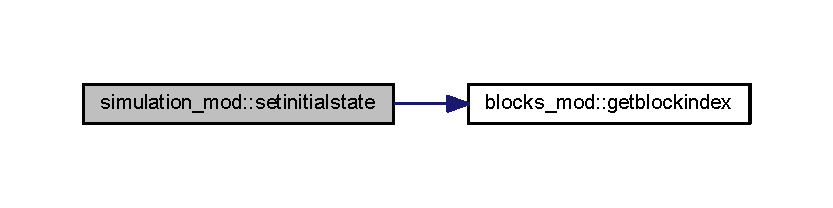
\includegraphics[width=350pt]{namespacesimulation__mod_a447c6d709de6aa360a65d39d660e627b_cgraph}
\end{center}
\end{figure}
\mbox{\Hypertarget{namespacesimulation__mod_acc5fa823c8dd599de8feda8988c224f2}\label{namespacesimulation__mod_acc5fa823c8dd599de8feda8988c224f2}} 
\index{simulation\+\_\+mod@{simulation\+\_\+mod}!settracermemory@{settracermemory}}
\index{settracermemory@{settracermemory}!simulation\+\_\+mod@{simulation\+\_\+mod}}
\subsubsection{\texorpdfstring{settracermemory()}{settracermemory()}}
{\footnotesize\ttfamily subroutine simulation\+\_\+mod\+::settracermemory (\begin{DoxyParamCaption}\item[{class(\mbox{\hyperlink{structsimulation__mod_1_1simulation__class}{simulation\+\_\+class}}), intent(in)}]{self,  }\item[{integer, intent(in), optional}]{ntrc }\end{DoxyParamCaption})\hspace{0.3cm}{\ttfamily [private]}}



Simulation method to account for Tracer memory consumption. 

\begin{DoxyAuthor}{Author}
Ricardo Birjukovs Canelas -\/ M\+A\+R\+E\+T\+EC 
\end{DoxyAuthor}


Definition at line 337 of file simulation.\+f90.


\begin{DoxyCode}
337     \textcolor{keywordtype}{implicit none}
338     \textcolor{keywordtype}{class}(simulation\_class), \textcolor{keywordtype}{intent(in)} :: self
339     \textcolor{keywordtype}{integer}, \textcolor{keywordtype}{optional}, \textcolor{keywordtype}{intent(in)} :: ntrc
340     \textcolor{keywordtype}{integer} :: sizem, i
341     sizem = 0
342     \textcolor{keywordflow}{do} i=1, \textcolor{keyword}{size}(dblock)
343         sizem = sizem + sizeof(dblock(i)%LTracer) \textcolor{comment}{!this accounts for the array structure}
344         sizem = sizem + sizeof(dummytracer)*dblock(i)%LTracer%getSize() \textcolor{comment}{!this accounts for the contents}
345 \textcolor{keywordflow}{    enddo}
346     \textcolor{keyword}{call }simmemory%setracer(sizem)
347     \textcolor{keywordflow}{if}(\textcolor{keyword}{present}(ntrc)) \textcolor{keywordflow}{then}
348         \textcolor{keyword}{call }simmemory%setNtrc(ntrc)
349         \textcolor{keyword}{call }simmemory%setsizeTrc(sizeof(dummytracer))
350 \textcolor{keywordflow}{    end if}
\end{DoxyCode}
\mbox{\Hypertarget{namespacesimulation__mod_a87a5141e4516b9610a6e4f0d2ff2d719}\label{namespacesimulation__mod_a87a5141e4516b9610a6e4f0d2ff2d719}} 
\index{simulation\+\_\+mod@{simulation\+\_\+mod}!togglesources@{togglesources}}
\index{togglesources@{togglesources}!simulation\+\_\+mod@{simulation\+\_\+mod}}
\subsubsection{\texorpdfstring{togglesources()}{togglesources()}}
{\footnotesize\ttfamily subroutine simulation\+\_\+mod\+::togglesources (\begin{DoxyParamCaption}\item[{class(\mbox{\hyperlink{structsimulation__mod_1_1simulation__class}{simulation\+\_\+class}}), intent(in)}]{self }\end{DoxyParamCaption})\hspace{0.3cm}{\ttfamily [private]}}



Simulation method to activate and deactivate Sources based on the GlobalSim\+Time. 

\begin{DoxyAuthor}{Author}
Ricardo Birjukovs Canelas -\/ M\+A\+R\+E\+T\+EC 
\end{DoxyAuthor}


Definition at line 176 of file simulation.\+f90.


\begin{DoxyCode}
176     \textcolor{keywordtype}{implicit none}
177     \textcolor{keywordtype}{class}(simulation\_class), \textcolor{keywordtype}{intent(in)} :: self
178     \textcolor{keywordtype}{integer} :: i
179     \textcolor{keywordflow}{do} i=1, \textcolor{keyword}{size}(dblock)
180         \textcolor{keyword}{call }dblock(i)%ToogleBlockSources()
181 \textcolor{keywordflow}{    enddo}
\end{DoxyCode}

\hypertarget{namespacesimulation__output__streamer__mod}{}\section{simulation\+\_\+output\+\_\+streamer\+\_\+mod Module Reference}
\label{namespacesimulation__output__streamer__mod}\index{simulation\+\_\+output\+\_\+streamer\+\_\+mod@{simulation\+\_\+output\+\_\+streamer\+\_\+mod}}


Defines a output file writer class with an object exposable to the Simulation This class is in charge of selectig the correct writter for the selected output file format.  


\subsection*{Data Types}
\begin{DoxyCompactItemize}
\item 
type \mbox{\hyperlink{structsimulation__output__streamer__mod_1_1output__streamer__class}{output\+\_\+streamer\+\_\+class}}
\end{DoxyCompactItemize}
\subsection*{Functions/\+Subroutines}
\begin{DoxyCompactItemize}
\item 
subroutine \mbox{\hyperlink{namespacesimulation__output__streamer__mod_a82c657d25adca9e0353ec9f87a4dd0c9}{initoutputstreamer}} (self)
\begin{DoxyCompactList}\small\item\em Initializes the Output writer object. \end{DoxyCompactList}\item 
subroutine \mbox{\hyperlink{namespacesimulation__output__streamer__mod_a4a290f3ef9ac868e173eab1ab9fd54b8}{writestepserial}} (self, blocks)
\begin{DoxyCompactList}\small\item\em Streamer method to call a simulation step writer. Writes binary X\+ML V\+TK format using an unstructured grid. \end{DoxyCompactList}\item 
subroutine \mbox{\hyperlink{namespacesimulation__output__streamer__mod_a1df8126a96e9b81ddf62841587728663}{writedomain}} (self, filename, bbox, npbbox, blocks)
\begin{DoxyCompactList}\small\item\em Public simulation domain writting routine. Writes binary X\+ML V\+TK format using an unstructured grid. \end{DoxyCompactList}\end{DoxyCompactItemize}
\subsection*{Variables}
\begin{DoxyCompactItemize}
\item 
type(\mbox{\hyperlink{structsimulation__output__streamer__mod_1_1output__streamer__class}{output\+\_\+streamer\+\_\+class}}), public \mbox{\hyperlink{namespacesimulation__output__streamer__mod_a6b95972f6387d7ce3231af3d25fedac5}{outputstreamer}}
\end{DoxyCompactItemize}


\subsection{Detailed Description}
Defines a output file writer class with an object exposable to the Simulation This class is in charge of selectig the correct writter for the selected output file format. 

\begin{DoxyAuthor}{Author}
Ricardo Birjukovs Canelas 
\end{DoxyAuthor}


\subsection{Function/\+Subroutine Documentation}
\mbox{\Hypertarget{namespacesimulation__output__streamer__mod_a82c657d25adca9e0353ec9f87a4dd0c9}\label{namespacesimulation__output__streamer__mod_a82c657d25adca9e0353ec9f87a4dd0c9}} 
\index{simulation\+\_\+output\+\_\+streamer\+\_\+mod@{simulation\+\_\+output\+\_\+streamer\+\_\+mod}!initoutputstreamer@{initoutputstreamer}}
\index{initoutputstreamer@{initoutputstreamer}!simulation\+\_\+output\+\_\+streamer\+\_\+mod@{simulation\+\_\+output\+\_\+streamer\+\_\+mod}}
\subsubsection{\texorpdfstring{initoutputstreamer()}{initoutputstreamer()}}
{\footnotesize\ttfamily subroutine simulation\+\_\+output\+\_\+streamer\+\_\+mod\+::initoutputstreamer (\begin{DoxyParamCaption}\item[{class(\mbox{\hyperlink{structsimulation__output__streamer__mod_1_1output__streamer__class}{output\+\_\+streamer\+\_\+class}}), intent(inout)}]{self }\end{DoxyParamCaption})\hspace{0.3cm}{\ttfamily [private]}}



Initializes the Output writer object. 

\begin{DoxyAuthor}{Author}
Ricardo Birjukovs Canelas -\/ M\+A\+R\+E\+T\+EC 
\end{DoxyAuthor}


Definition at line 54 of file simulation\+\_\+output\+\_\+streamer.\+f90.


\begin{DoxyCode}
54     \textcolor{keywordtype}{implicit none}
55     \textcolor{keywordtype}{class}(output\_streamer\_class), \textcolor{keywordtype}{intent(inout)} :: self
56     self%OutputFormat = globals%Parameters%OutputFormat
57     \textcolor{keywordflow}{if} (self%OutputFormat == 2) \textcolor{keywordflow}{then} \textcolor{comment}{!VTK file selected}
58         \textcolor{keyword}{call }vtkwritter%initialize()
59 \textcolor{keywordflow}{    end if}
\end{DoxyCode}
\mbox{\Hypertarget{namespacesimulation__output__streamer__mod_a1df8126a96e9b81ddf62841587728663}\label{namespacesimulation__output__streamer__mod_a1df8126a96e9b81ddf62841587728663}} 
\index{simulation\+\_\+output\+\_\+streamer\+\_\+mod@{simulation\+\_\+output\+\_\+streamer\+\_\+mod}!writedomain@{writedomain}}
\index{writedomain@{writedomain}!simulation\+\_\+output\+\_\+streamer\+\_\+mod@{simulation\+\_\+output\+\_\+streamer\+\_\+mod}}
\subsubsection{\texorpdfstring{writedomain()}{writedomain()}}
{\footnotesize\ttfamily subroutine simulation\+\_\+output\+\_\+streamer\+\_\+mod\+::writedomain (\begin{DoxyParamCaption}\item[{class(\mbox{\hyperlink{structsimulation__output__streamer__mod_1_1output__streamer__class}{output\+\_\+streamer\+\_\+class}}), intent(inout)}]{self,  }\item[{type(string), intent(in)}]{filename,  }\item[{class(\mbox{\hyperlink{structboundingbox__mod_1_1boundingbox__class}{boundingbox\+\_\+class}}), intent(in)}]{bbox,  }\item[{integer, intent(in)}]{npbbox,  }\item[{class(\mbox{\hyperlink{structblocks__mod_1_1block__class}{block\+\_\+class}}), dimension(\+:), intent(in)}]{blocks }\end{DoxyParamCaption})\hspace{0.3cm}{\ttfamily [private]}}



Public simulation domain writting routine. Writes binary X\+ML V\+TK format using an unstructured grid. 

\begin{DoxyAuthor}{Author}
Ricardo Birjukovs Canelas -\/ M\+A\+R\+E\+T\+EC 
\end{DoxyAuthor}

\begin{DoxyParams}[1]{Parameters}
\mbox{\tt in}  & {\em self,filename,bbox,npbbox,blocks} & \\
\hline
\mbox{\tt in}  & {\em filename} & name of the case to add\\
\hline
\mbox{\tt in}  & {\em bbox} & Case bounding box\\
\hline
\mbox{\tt in}  & {\em npbbox} & number of points of the bbox geometry\\
\hline
\mbox{\tt in}  & {\em blocks} & Case Blocks \\
\hline
\end{DoxyParams}


Definition at line 93 of file simulation\+\_\+output\+\_\+streamer.\+f90.


\begin{DoxyCode}
93     \textcolor{keywordtype}{implicit none}
94     \textcolor{keywordtype}{class}(output\_streamer\_class), \textcolor{keywordtype}{intent(inout)} :: self
95     \textcolor{keywordtype}{type}(string), \textcolor{keywordtype}{intent(in)} :: filename
96     \textcolor{keywordtype}{class}(boundingbox\_class), \textcolor{keywordtype}{intent(in)} :: bbox
97     \textcolor{keywordtype}{integer}, \textcolor{keywordtype}{intent(in)} :: npbbox
98     \textcolor{keywordtype}{class}(block\_class), \textcolor{keywordtype}{dimension(:)}, \textcolor{keywordtype}{intent(in)} :: blocks
99     
100     \textcolor{keywordflow}{if} (self%OutputFormat == 2) \textcolor{keywordflow}{then} \textcolor{comment}{!VTK file selected}
101         \textcolor{keyword}{call }vtkwritter%Domain(filename, bbox, npbbox, blocks)
102 \textcolor{keywordflow}{    end if}
103     
\end{DoxyCode}
\mbox{\Hypertarget{namespacesimulation__output__streamer__mod_a4a290f3ef9ac868e173eab1ab9fd54b8}\label{namespacesimulation__output__streamer__mod_a4a290f3ef9ac868e173eab1ab9fd54b8}} 
\index{simulation\+\_\+output\+\_\+streamer\+\_\+mod@{simulation\+\_\+output\+\_\+streamer\+\_\+mod}!writestepserial@{writestepserial}}
\index{writestepserial@{writestepserial}!simulation\+\_\+output\+\_\+streamer\+\_\+mod@{simulation\+\_\+output\+\_\+streamer\+\_\+mod}}
\subsubsection{\texorpdfstring{writestepserial()}{writestepserial()}}
{\footnotesize\ttfamily subroutine simulation\+\_\+output\+\_\+streamer\+\_\+mod\+::writestepserial (\begin{DoxyParamCaption}\item[{class(\mbox{\hyperlink{structsimulation__output__streamer__mod_1_1output__streamer__class}{output\+\_\+streamer\+\_\+class}}), intent(inout)}]{self,  }\item[{class(\mbox{\hyperlink{structblocks__mod_1_1block__class}{block\+\_\+class}}), dimension(\+:), intent(in)}]{blocks }\end{DoxyParamCaption})\hspace{0.3cm}{\ttfamily [private]}}



Streamer method to call a simulation step writer. Writes binary X\+ML V\+TK format using an unstructured grid. 

\begin{DoxyAuthor}{Author}
Ricardo Birjukovs Canelas -\/ M\+A\+R\+E\+T\+EC 
\end{DoxyAuthor}

\begin{DoxyParams}[1]{Parameters}
\mbox{\tt in}  & {\em self,blocks} & \\
\hline
\mbox{\tt in}  & {\em blocks} & Case Blocks \\
\hline
\end{DoxyParams}


Definition at line 70 of file simulation\+\_\+output\+\_\+streamer.\+f90.


\begin{DoxyCode}
70     \textcolor{keywordtype}{implicit none}
71     \textcolor{keywordtype}{class}(output\_streamer\_class), \textcolor{keywordtype}{intent(inout)} :: self   
72     \textcolor{keywordtype}{class}(block\_class), \textcolor{keywordtype}{dimension(:)}, \textcolor{keywordtype}{intent(in)} :: blocks
73     \textcolor{keywordtype}{type}(string) :: filename
74     
75     filename = globals%Names%casename//\textcolor{stringliteral}{'\_'}//int2str(\textcolor{stringliteral}{'(i5.5)'},globals%Sim%getnumoutfile())
76     
77     \textcolor{keywordflow}{if} (self%OutputFormat == 2) \textcolor{keywordflow}{then} \textcolor{comment}{!VTK file selected}
78         \textcolor{keyword}{call }vtkwritter%TracerSerial(filename, blocks)
79 \textcolor{keywordflow}{    end if}
80     
81     \textcolor{keyword}{call }globals%Sim%increment\_numoutfile()
82     
\end{DoxyCode}


\subsection{Variable Documentation}
\mbox{\Hypertarget{namespacesimulation__output__streamer__mod_a6b95972f6387d7ce3231af3d25fedac5}\label{namespacesimulation__output__streamer__mod_a6b95972f6387d7ce3231af3d25fedac5}} 
\index{simulation\+\_\+output\+\_\+streamer\+\_\+mod@{simulation\+\_\+output\+\_\+streamer\+\_\+mod}!outputstreamer@{outputstreamer}}
\index{outputstreamer@{outputstreamer}!simulation\+\_\+output\+\_\+streamer\+\_\+mod@{simulation\+\_\+output\+\_\+streamer\+\_\+mod}}
\subsubsection{\texorpdfstring{outputstreamer}{outputstreamer}}
{\footnotesize\ttfamily type(\mbox{\hyperlink{structsimulation__output__streamer__mod_1_1output__streamer__class}{output\+\_\+streamer\+\_\+class}}), public simulation\+\_\+output\+\_\+streamer\+\_\+mod\+::outputstreamer}



Definition at line 39 of file simulation\+\_\+output\+\_\+streamer.\+f90.


\begin{DoxyCode}
39     \textcolor{keywordtype}{type}(output\_streamer\_class) :: OutputStreamer
\end{DoxyCode}

\hypertarget{namespacesimulation__precision__mod}{}\section{simulation\+\_\+precision\+\_\+mod Module Reference}
\label{namespacesimulation__precision__mod}\index{simulation\+\_\+precision\+\_\+mod@{simulation\+\_\+precision\+\_\+mod}}


Module to control the precision of the variables trough the project.  


\subsection*{Variables}
\begin{DoxyCompactItemize}
\item 
integer, parameter \hyperlink{namespacesimulation__precision__mod_a15b1ab993f9b11430e9d9d3dc6c77614}{sp} = kind(1.\+\_\+\+R4P)
\begin{DoxyCompactList}\small\item\em Simple precision definition switch. \end{DoxyCompactList}\item 
integer, parameter \hyperlink{namespacesimulation__precision__mod_a4d49b0033a5e2bc6693c5b2dfb63a032}{dp} = kind(1.\+\_\+\+R8P)
\begin{DoxyCompactList}\small\item\em Double precision definition switch. \end{DoxyCompactList}\item 
integer, parameter, public \hyperlink{namespacesimulation__precision__mod_aaff1ddf996761a1e11e787d63e1612f6}{prec} = \hyperlink{namespacesimulation__precision__mod_a15b1ab993f9b11430e9d9d3dc6c77614}{sp}
\item 
integer, parameter, public \hyperlink{namespacesimulation__precision__mod_a3833ad1bc52c3738ac861591b7492737}{prec\+\_\+time} = \hyperlink{namespacesimulation__precision__mod_a15b1ab993f9b11430e9d9d3dc6c77614}{sp}
\item 
integer, parameter, public \hyperlink{namespacesimulation__precision__mod_ad515822198607dfee68a6ed8b246c7da}{prec\+\_\+wrt} = \hyperlink{namespacesimulation__precision__mod_a15b1ab993f9b11430e9d9d3dc6c77614}{sp}
\item 
real(\hyperlink{namespacesimulation__precision__mod_aaff1ddf996761a1e11e787d63e1612f6}{prec}), parameter, public \hyperlink{namespacesimulation__precision__mod_a1fb0f91226452bb43d4c61cae32a9a6d}{missing\+\_\+value\+\_\+default} = -\/9999.\+0\+\_\+dp
\item 
real(\hyperlink{namespacesimulation__precision__mod_aaff1ddf996761a1e11e787d63e1612f6}{prec}), parameter, public \hyperlink{namespacesimulation__precision__mod_a39845d8a0d331a7b9225feb5fe19ba3b}{mv} = M\+I\+S\+S\+I\+N\+G\+\_\+\+V\+A\+L\+U\+E\+\_\+\+D\+E\+F\+A\+U\+LT
\item 
real(\hyperlink{namespacesimulation__precision__mod_aaff1ddf996761a1e11e787d63e1612f6}{prec}), parameter, public \hyperlink{namespacesimulation__precision__mod_abcad51274c804cb573d8f5720c5dfa05}{mv\+\_\+int} = int(M\+I\+S\+S\+I\+N\+G\+\_\+\+V\+A\+L\+U\+E\+\_\+\+D\+E\+F\+A\+U\+LT)
\item 
real(\hyperlink{namespacesimulation__precision__mod_aaff1ddf996761a1e11e787d63e1612f6}{prec}), parameter, public \hyperlink{namespacesimulation__precision__mod_ae3222dd2d51f6b7221be1ca1c70e3e6c}{err\+\_\+dist} = 1\+E8\+\_\+dp
\item 
integer, parameter, public \hyperlink{namespacesimulation__precision__mod_a82a4b689dc26018c961193b991c489d4}{err\+\_\+ind} = -\/1
\item 
integer, parameter, public \hyperlink{namespacesimulation__precision__mod_a8a3305091ff953708508525398aa7129}{char\+\_\+len} = 99
\end{DoxyCompactItemize}


\subsection{Detailed Description}
Module to control the precision of the variables trough the project. 

\begin{DoxyAuthor}{Author}
Ricardo Birjukovs Canelas 
\end{DoxyAuthor}


\subsection{Variable Documentation}
\mbox{\Hypertarget{namespacesimulation__precision__mod_a8a3305091ff953708508525398aa7129}\label{namespacesimulation__precision__mod_a8a3305091ff953708508525398aa7129}} 
\index{simulation\+\_\+precision\+\_\+mod@{simulation\+\_\+precision\+\_\+mod}!char\+\_\+len@{char\+\_\+len}}
\index{char\+\_\+len@{char\+\_\+len}!simulation\+\_\+precision\+\_\+mod@{simulation\+\_\+precision\+\_\+mod}}
\subsubsection{\texorpdfstring{char\+\_\+len}{char\_len}}
{\footnotesize\ttfamily integer, parameter, public simulation\+\_\+precision\+\_\+mod\+::char\+\_\+len = 99}

\mbox{\Hypertarget{namespacesimulation__precision__mod_a4d49b0033a5e2bc6693c5b2dfb63a032}\label{namespacesimulation__precision__mod_a4d49b0033a5e2bc6693c5b2dfb63a032}} 
\index{simulation\+\_\+precision\+\_\+mod@{simulation\+\_\+precision\+\_\+mod}!dp@{dp}}
\index{dp@{dp}!simulation\+\_\+precision\+\_\+mod@{simulation\+\_\+precision\+\_\+mod}}
\subsubsection{\texorpdfstring{dp}{dp}}
{\footnotesize\ttfamily integer, parameter simulation\+\_\+precision\+\_\+mod\+::dp = kind(1.\+\_\+\+R8P)\hspace{0.3cm}{\ttfamily [private]}}



Double precision definition switch. 

\mbox{\Hypertarget{namespacesimulation__precision__mod_ae3222dd2d51f6b7221be1ca1c70e3e6c}\label{namespacesimulation__precision__mod_ae3222dd2d51f6b7221be1ca1c70e3e6c}} 
\index{simulation\+\_\+precision\+\_\+mod@{simulation\+\_\+precision\+\_\+mod}!err\+\_\+dist@{err\+\_\+dist}}
\index{err\+\_\+dist@{err\+\_\+dist}!simulation\+\_\+precision\+\_\+mod@{simulation\+\_\+precision\+\_\+mod}}
\subsubsection{\texorpdfstring{err\+\_\+dist}{err\_dist}}
{\footnotesize\ttfamily real(\hyperlink{namespacesimulation__precision__mod_aaff1ddf996761a1e11e787d63e1612f6}{prec}), parameter, public simulation\+\_\+precision\+\_\+mod\+::err\+\_\+dist = 1\+E8\+\_\+dp}

\mbox{\Hypertarget{namespacesimulation__precision__mod_a82a4b689dc26018c961193b991c489d4}\label{namespacesimulation__precision__mod_a82a4b689dc26018c961193b991c489d4}} 
\index{simulation\+\_\+precision\+\_\+mod@{simulation\+\_\+precision\+\_\+mod}!err\+\_\+ind@{err\+\_\+ind}}
\index{err\+\_\+ind@{err\+\_\+ind}!simulation\+\_\+precision\+\_\+mod@{simulation\+\_\+precision\+\_\+mod}}
\subsubsection{\texorpdfstring{err\+\_\+ind}{err\_ind}}
{\footnotesize\ttfamily integer, parameter, public simulation\+\_\+precision\+\_\+mod\+::err\+\_\+ind = -\/1}

\mbox{\Hypertarget{namespacesimulation__precision__mod_a1fb0f91226452bb43d4c61cae32a9a6d}\label{namespacesimulation__precision__mod_a1fb0f91226452bb43d4c61cae32a9a6d}} 
\index{simulation\+\_\+precision\+\_\+mod@{simulation\+\_\+precision\+\_\+mod}!missing\+\_\+value\+\_\+default@{missing\+\_\+value\+\_\+default}}
\index{missing\+\_\+value\+\_\+default@{missing\+\_\+value\+\_\+default}!simulation\+\_\+precision\+\_\+mod@{simulation\+\_\+precision\+\_\+mod}}
\subsubsection{\texorpdfstring{missing\+\_\+value\+\_\+default}{missing\_value\_default}}
{\footnotesize\ttfamily real(\hyperlink{namespacesimulation__precision__mod_aaff1ddf996761a1e11e787d63e1612f6}{prec}), parameter, public simulation\+\_\+precision\+\_\+mod\+::missing\+\_\+value\+\_\+default = -\/9999.\+0\+\_\+dp}

\mbox{\Hypertarget{namespacesimulation__precision__mod_a39845d8a0d331a7b9225feb5fe19ba3b}\label{namespacesimulation__precision__mod_a39845d8a0d331a7b9225feb5fe19ba3b}} 
\index{simulation\+\_\+precision\+\_\+mod@{simulation\+\_\+precision\+\_\+mod}!mv@{mv}}
\index{mv@{mv}!simulation\+\_\+precision\+\_\+mod@{simulation\+\_\+precision\+\_\+mod}}
\subsubsection{\texorpdfstring{mv}{mv}}
{\footnotesize\ttfamily real(\hyperlink{namespacesimulation__precision__mod_aaff1ddf996761a1e11e787d63e1612f6}{prec}), parameter, public simulation\+\_\+precision\+\_\+mod\+::mv = M\+I\+S\+S\+I\+N\+G\+\_\+\+V\+A\+L\+U\+E\+\_\+\+D\+E\+F\+A\+U\+LT}

\mbox{\Hypertarget{namespacesimulation__precision__mod_abcad51274c804cb573d8f5720c5dfa05}\label{namespacesimulation__precision__mod_abcad51274c804cb573d8f5720c5dfa05}} 
\index{simulation\+\_\+precision\+\_\+mod@{simulation\+\_\+precision\+\_\+mod}!mv\+\_\+int@{mv\+\_\+int}}
\index{mv\+\_\+int@{mv\+\_\+int}!simulation\+\_\+precision\+\_\+mod@{simulation\+\_\+precision\+\_\+mod}}
\subsubsection{\texorpdfstring{mv\+\_\+int}{mv\_int}}
{\footnotesize\ttfamily real(\hyperlink{namespacesimulation__precision__mod_aaff1ddf996761a1e11e787d63e1612f6}{prec}), parameter, public simulation\+\_\+precision\+\_\+mod\+::mv\+\_\+int = int(M\+I\+S\+S\+I\+N\+G\+\_\+\+V\+A\+L\+U\+E\+\_\+\+D\+E\+F\+A\+U\+LT)}

\mbox{\Hypertarget{namespacesimulation__precision__mod_aaff1ddf996761a1e11e787d63e1612f6}\label{namespacesimulation__precision__mod_aaff1ddf996761a1e11e787d63e1612f6}} 
\index{simulation\+\_\+precision\+\_\+mod@{simulation\+\_\+precision\+\_\+mod}!prec@{prec}}
\index{prec@{prec}!simulation\+\_\+precision\+\_\+mod@{simulation\+\_\+precision\+\_\+mod}}
\subsubsection{\texorpdfstring{prec}{prec}}
{\footnotesize\ttfamily integer, parameter, public simulation\+\_\+precision\+\_\+mod\+::prec = \hyperlink{namespacesimulation__precision__mod_a15b1ab993f9b11430e9d9d3dc6c77614}{sp}}

\mbox{\Hypertarget{namespacesimulation__precision__mod_a3833ad1bc52c3738ac861591b7492737}\label{namespacesimulation__precision__mod_a3833ad1bc52c3738ac861591b7492737}} 
\index{simulation\+\_\+precision\+\_\+mod@{simulation\+\_\+precision\+\_\+mod}!prec\+\_\+time@{prec\+\_\+time}}
\index{prec\+\_\+time@{prec\+\_\+time}!simulation\+\_\+precision\+\_\+mod@{simulation\+\_\+precision\+\_\+mod}}
\subsubsection{\texorpdfstring{prec\+\_\+time}{prec\_time}}
{\footnotesize\ttfamily integer, parameter, public simulation\+\_\+precision\+\_\+mod\+::prec\+\_\+time = \hyperlink{namespacesimulation__precision__mod_a15b1ab993f9b11430e9d9d3dc6c77614}{sp}}

\mbox{\Hypertarget{namespacesimulation__precision__mod_ad515822198607dfee68a6ed8b246c7da}\label{namespacesimulation__precision__mod_ad515822198607dfee68a6ed8b246c7da}} 
\index{simulation\+\_\+precision\+\_\+mod@{simulation\+\_\+precision\+\_\+mod}!prec\+\_\+wrt@{prec\+\_\+wrt}}
\index{prec\+\_\+wrt@{prec\+\_\+wrt}!simulation\+\_\+precision\+\_\+mod@{simulation\+\_\+precision\+\_\+mod}}
\subsubsection{\texorpdfstring{prec\+\_\+wrt}{prec\_wrt}}
{\footnotesize\ttfamily integer, parameter, public simulation\+\_\+precision\+\_\+mod\+::prec\+\_\+wrt = \hyperlink{namespacesimulation__precision__mod_a15b1ab993f9b11430e9d9d3dc6c77614}{sp}}

\mbox{\Hypertarget{namespacesimulation__precision__mod_a15b1ab993f9b11430e9d9d3dc6c77614}\label{namespacesimulation__precision__mod_a15b1ab993f9b11430e9d9d3dc6c77614}} 
\index{simulation\+\_\+precision\+\_\+mod@{simulation\+\_\+precision\+\_\+mod}!sp@{sp}}
\index{sp@{sp}!simulation\+\_\+precision\+\_\+mod@{simulation\+\_\+precision\+\_\+mod}}
\subsubsection{\texorpdfstring{sp}{sp}}
{\footnotesize\ttfamily integer, parameter simulation\+\_\+precision\+\_\+mod\+::sp = kind(1.\+\_\+\+R4P)\hspace{0.3cm}{\ttfamily [private]}}



Simple precision definition switch. 


\hypertarget{namespacesources__list__mod}{}\section{sources\+\_\+list\+\_\+mod Module Reference}
\label{namespacesources__list__mod}\index{sources\+\_\+list\+\_\+mod@{sources\+\_\+list\+\_\+mod}}


Module to hold the Sources linked list class and its methods. This class defines a double linked list to store any variable type, but with specific methods with type guards for Source objects. The class allows for insertion, deletion and iteration of the desired contents.  


\subsection*{Data Types}
\begin{DoxyCompactItemize}
\item 
type \mbox{\hyperlink{structsources__list__mod_1_1sourcelist__class}{sourcelist\+\_\+class}}
\end{DoxyCompactItemize}
\subsection*{Functions/\+Subroutines}
\begin{DoxyCompactItemize}
\item 
subroutine \mbox{\hyperlink{namespacesources__list__mod_ac9ab885c3cc6a38c8b12b694e40a11e1}{print\+\_\+sourcelist}} (this)
\begin{DoxyCompactList}\small\item\em Method that prints all the links of the list. \end{DoxyCompactList}\item 
subroutine \mbox{\hyperlink{namespacesources__list__mod_aad2008cc97f57cd85297d3f3d81fac39}{print\+\_\+sourcelistcurrent}} (this)
\begin{DoxyCompactList}\small\item\em Method that prints the current link of the list. \end{DoxyCompactList}\end{DoxyCompactItemize}


\subsection{Detailed Description}
Module to hold the Sources linked list class and its methods. This class defines a double linked list to store any variable type, but with specific methods with type guards for Source objects. The class allows for insertion, deletion and iteration of the desired contents. 

\begin{DoxyAuthor}{Author}
Ricardo Birjukovs Canelas 
\end{DoxyAuthor}


\subsection{Function/\+Subroutine Documentation}
\mbox{\Hypertarget{namespacesources__list__mod_ac9ab885c3cc6a38c8b12b694e40a11e1}\label{namespacesources__list__mod_ac9ab885c3cc6a38c8b12b694e40a11e1}} 
\index{sources\+\_\+list\+\_\+mod@{sources\+\_\+list\+\_\+mod}!print\+\_\+sourcelist@{print\+\_\+sourcelist}}
\index{print\+\_\+sourcelist@{print\+\_\+sourcelist}!sources\+\_\+list\+\_\+mod@{sources\+\_\+list\+\_\+mod}}
\subsubsection{\texorpdfstring{print\+\_\+sourcelist()}{print\_sourcelist()}}
{\footnotesize\ttfamily subroutine sources\+\_\+list\+\_\+mod\+::print\+\_\+sourcelist (\begin{DoxyParamCaption}\item[{class(\mbox{\hyperlink{structsources__list__mod_1_1sourcelist__class}{sourcelist\+\_\+class}}), intent(in)}]{this }\end{DoxyParamCaption})\hspace{0.3cm}{\ttfamily [private]}}



Method that prints all the links of the list. 

\begin{DoxyAuthor}{Author}
Ricardo Birjukovs Canelas -\/ M\+A\+R\+E\+T\+EC 
\end{DoxyAuthor}


Definition at line 47 of file sources\+\_\+list.\+f90.


\begin{DoxyCode}
47     \textcolor{keywordtype}{class}(sourceList\_class), \textcolor{keywordtype}{intent(in)} :: this
48     \textcolor{keywordtype}{class}(*), \textcolor{keywordtype}{pointer} :: curr
49     \textcolor{keyword}{call }this%reset()               \textcolor{comment}{! reset list iterator}
50     \textcolor{keywordflow}{do} \textcolor{keywordflow}{while}(this%moreValues())     \textcolor{comment}{! loop while there are values to print}
51         \textcolor{keyword}{call }this%printCurrent()
52         \textcolor{keyword}{call }this%next()            \textcolor{comment}{! increment the list iterator}
53 \textcolor{keywordflow}{    end do}
54     \textcolor{keyword}{call }this%reset()               \textcolor{comment}{! reset list iterator}
\end{DoxyCode}
\mbox{\Hypertarget{namespacesources__list__mod_aad2008cc97f57cd85297d3f3d81fac39}\label{namespacesources__list__mod_aad2008cc97f57cd85297d3f3d81fac39}} 
\index{sources\+\_\+list\+\_\+mod@{sources\+\_\+list\+\_\+mod}!print\+\_\+sourcelistcurrent@{print\+\_\+sourcelistcurrent}}
\index{print\+\_\+sourcelistcurrent@{print\+\_\+sourcelistcurrent}!sources\+\_\+list\+\_\+mod@{sources\+\_\+list\+\_\+mod}}
\subsubsection{\texorpdfstring{print\+\_\+sourcelistcurrent()}{print\_sourcelistcurrent()}}
{\footnotesize\ttfamily subroutine sources\+\_\+list\+\_\+mod\+::print\+\_\+sourcelistcurrent (\begin{DoxyParamCaption}\item[{class(\mbox{\hyperlink{structsources__list__mod_1_1sourcelist__class}{sourcelist\+\_\+class}}), intent(in)}]{this }\end{DoxyParamCaption})\hspace{0.3cm}{\ttfamily [private]}}



Method that prints the current link of the list. 

\begin{DoxyAuthor}{Author}
Ricardo Birjukovs Canelas -\/ M\+A\+R\+E\+T\+EC 
\end{DoxyAuthor}


Definition at line 63 of file sources\+\_\+list.\+f90.


\begin{DoxyCode}
63     \textcolor{keywordtype}{class}(sourceList\_class), \textcolor{keywordtype}{intent(in)} :: this
64     \textcolor{keywordtype}{class}(*), \textcolor{keywordtype}{pointer} :: curr
65     \textcolor{keywordtype}{type}(string) :: outext
66     curr => this%currentValue() \textcolor{comment}{! get current value}
67     \textcolor{keywordflow}{select type}(curr)
68 \textcolor{keywordflow}{    class is} (source\_class)
69         \textcolor{keyword}{call }curr%print()
70 \textcolor{keywordflow}{        class default}
71         outext = \textcolor{stringliteral}{'[sourceList\_class::print] Unexepected type of content, not a Source'}
72         \textcolor{keyword}{call }log%put(outext)
73         stop
74 \textcolor{keywordflow}{    end select}
\end{DoxyCode}

\hypertarget{namespacesources__mod}{}\section{sources\+\_\+mod Module Reference}
\label{namespacesources__mod}\index{sources\+\_\+mod@{sources\+\_\+mod}}


Module that defines a source class and related methods.  


\subsection*{Data Types}
\begin{DoxyCompactItemize}
\item 
type \mbox{\hyperlink{structsources__mod_1_1source__class}{source\+\_\+class}}
\begin{DoxyCompactList}\small\item\em Type -\/ The source class. \end{DoxyCompactList}\item 
type \mbox{\hyperlink{structsources__mod_1_1source__group__class}{source\+\_\+group\+\_\+class}}
\item 
type \mbox{\hyperlink{structsources__mod_1_1source__par}{source\+\_\+par}}
\item 
type \mbox{\hyperlink{structsources__mod_1_1source__prop}{source\+\_\+prop}}
\begin{DoxyCompactList}\small\item\em Type -\/ material properties of a source object. \end{DoxyCompactList}\item 
type \mbox{\hyperlink{structsources__mod_1_1source__state}{source\+\_\+state}}
\begin{DoxyCompactList}\small\item\em Type -\/ state variables of a source object. \end{DoxyCompactList}\item 
type \mbox{\hyperlink{structsources__mod_1_1source__stats}{source\+\_\+stats}}
\begin{DoxyCompactList}\small\item\em Type -\/ statistical variables of a source object. \end{DoxyCompactList}\item 
type \mbox{\hyperlink{structsources__mod_1_1source__stencil}{source\+\_\+stencil}}
\begin{DoxyCompactList}\small\item\em Type -\/ holder for the tracer creation stencil of the source. \end{DoxyCompactList}\end{DoxyCompactItemize}
\subsection*{Functions/\+Subroutines}
\begin{DoxyCompactItemize}
\item 
subroutine \mbox{\hyperlink{namespacesources__mod_a6da3303e5c39d77c0111ec50623bf5fe}{initsources}} (self, nsources)
\begin{DoxyCompactList}\small\item\em source allocation routine -\/ allocates sources objects \end{DoxyCompactList}\item 
subroutine \mbox{\hyperlink{namespacesources__mod_aee745aa084adcfa41ecfc3469b90aa8e}{killsources}} (self)
\begin{DoxyCompactList}\small\item\em source group destructor -\/ deallocates sources objects \end{DoxyCompactList}\item 
subroutine \mbox{\hyperlink{namespacesources__mod_a683ca7e4aca7a0050aad9f506569fca9}{linkproperty}} (src, ptype, pname)
\begin{DoxyCompactList}\small\item\em source property setting proceadure -\/ initializes Source variables \end{DoxyCompactList}\item 
subroutine \mbox{\hyperlink{namespacesources__mod_aa76f16f8ee96bc86b553aa54d420321c}{setpropertynames}} (self, srcid\+\_\+str, ptype, pname)
\begin{DoxyCompactList}\small\item\em source property setting routine, calls source by id to set its properties \end{DoxyCompactList}\item 
subroutine \mbox{\hyperlink{namespacesources__mod_abbb4557b46c533439fe258cecf31a76c}{setpropertyatributes}} (src, pname, pvalue)
\begin{DoxyCompactList}\small\item\em source property atribute setting proceadure -\/ initializes Source variables \end{DoxyCompactList}\item 
subroutine \mbox{\hyperlink{namespacesources__mod_a6fcfcb690cd1b9375915b01f7ddbe801}{check}} (self)
\begin{DoxyCompactList}\small\item\em Method that checks for the consistency of the Source properties. \end{DoxyCompactList}\item 
subroutine \mbox{\hyperlink{namespacesources__mod_a6dcf7a3e3ccf75e01853df166231d484}{initializesource}} (src, id, name, emitting\+\_\+rate, start, finish, source\+\_\+geometry, shapetype)
\begin{DoxyCompactList}\small\item\em source inititialization proceadure -\/ initializes Source variables \end{DoxyCompactList}\item 
logical function \mbox{\hyperlink{namespacesources__mod_ac4e4f33da78d030e1b56a48789da6a05}{isparticulate}} (self)
\begin{DoxyCompactList}\small\item\em Returns particulate status of this Source, i.\+e, true if the emitted Tracers are actually a collection of particles with an evolving concentration. \end{DoxyCompactList}\item 
subroutine \mbox{\hyperlink{namespacesources__mod_a9a62c41b71d2d6ad85def74087542ef5}{setotalnp}} (self)
\begin{DoxyCompactList}\small\item\em method that sets the total number of tracers a source will potentially create ${NP}_{total}^{source-i}=int((T_{end}^{source-i}-T_{start}^{source-i})/(Dt/{Rate}^{source-i})*{NP}_{emission}^{source-i})$ \end{DoxyCompactList}\item 
subroutine \mbox{\hyperlink{namespacesources__mod_a641fe9ecc295e486a714c1aaa133d991}{printsource}} (src)
\begin{DoxyCompactList}\small\item\em source print routine -\/ prints a source info on console/log \end{DoxyCompactList}\end{DoxyCompactItemize}
\subsection*{Variables}
\begin{DoxyCompactItemize}
\item 
type(\mbox{\hyperlink{structsources__mod_1_1source__group__class}{source\+\_\+group\+\_\+class}}), public \mbox{\hyperlink{namespacesources__mod_ab04ea8c02cdf83a1a356c8710ae811d5}{tempsources}}
\begin{DoxyCompactList}\small\item\em Temporary Source array, used exclusively for building the case from a description file. \end{DoxyCompactList}\end{DoxyCompactItemize}


\subsection{Detailed Description}
Module that defines a source class and related methods. 

\begin{DoxyAuthor}{Author}
Ricardo Birjukovs Canelas 
\end{DoxyAuthor}


\subsection{Function/\+Subroutine Documentation}
\mbox{\Hypertarget{namespacesources__mod_a6fcfcb690cd1b9375915b01f7ddbe801}\label{namespacesources__mod_a6fcfcb690cd1b9375915b01f7ddbe801}} 
\index{sources\+\_\+mod@{sources\+\_\+mod}!check@{check}}
\index{check@{check}!sources\+\_\+mod@{sources\+\_\+mod}}
\subsubsection{\texorpdfstring{check()}{check()}}
{\footnotesize\ttfamily subroutine sources\+\_\+mod\+::check (\begin{DoxyParamCaption}\item[{class(\mbox{\hyperlink{structsources__mod_1_1source__class}{source\+\_\+class}}), intent(in)}]{self }\end{DoxyParamCaption})\hspace{0.3cm}{\ttfamily [private]}}



Method that checks for the consistency of the Source properties. 

\begin{DoxyAuthor}{Author}
Ricardo Birjukovs Canelas -\/ M\+A\+R\+E\+T\+EC 
\end{DoxyAuthor}


Definition at line 241 of file sources.\+f90.


\begin{DoxyCode}
241     \textcolor{keywordtype}{implicit none}
242     \textcolor{keywordtype}{class}(source\_class), \textcolor{keywordtype}{intent(in)} :: self
243     \textcolor{keywordtype}{type}(string) :: outext, temp(2)
244     \textcolor{keywordtype}{logical} :: failed
245     failed = .false.
246     temp(1) = self%par%id
247     \textcolor{keywordflow}{if} (self%prop%radius == mv) \textcolor{keywordflow}{then}
248         failed = .true.
249         temp(2) = \textcolor{stringliteral}{'radius'}
250     \textcolor{keywordflow}{elseif} (self%prop%density == mv) \textcolor{keywordflow}{then}
251         failed = .true.
252         temp(2) = \textcolor{stringliteral}{'density'}
253     \textcolor{keywordflow}{elseif} (self%prop%condition == mv) \textcolor{keywordflow}{then}
254         failed = .true.
255         temp(2) = \textcolor{stringliteral}{'condition'}
256     \textcolor{keywordflow}{elseif} (self%prop%degrd\_rate == mv) \textcolor{keywordflow}{then}
257         failed = .true.
258         temp(2) = \textcolor{stringliteral}{'degradation rate'}
259     \textcolor{keywordflow}{elseif} (self%prop%particulate) \textcolor{keywordflow}{then}
260         \textcolor{keywordflow}{if} (self%prop%pt\_radius == mv) \textcolor{keywordflow}{then}
261             failed = .true.
262             temp(2) = \textcolor{stringliteral}{'particle radius'}
263         \textcolor{keywordflow}{elseif} (self%prop%ini\_concentration == mv) \textcolor{keywordflow}{then}
264             failed = .true.
265             temp(2) = \textcolor{stringliteral}{'initial concentration'}
266 \textcolor{keywordflow}{        end if}
267 \textcolor{keywordflow}{    end if}
268     \textcolor{keywordflow}{if} (failed) \textcolor{keywordflow}{then}
269         outext = \textcolor{stringliteral}{'Source'}//temp(1)//\textcolor{stringliteral}{' '}//temp(2)//\textcolor{stringliteral}{' is not set, stoping'}
270         \textcolor{keyword}{call }log%put(outext)
271         stop
272 \textcolor{keywordflow}{    end if}
\end{DoxyCode}
\mbox{\Hypertarget{namespacesources__mod_a6dcf7a3e3ccf75e01853df166231d484}\label{namespacesources__mod_a6dcf7a3e3ccf75e01853df166231d484}} 
\index{sources\+\_\+mod@{sources\+\_\+mod}!initializesource@{initializesource}}
\index{initializesource@{initializesource}!sources\+\_\+mod@{sources\+\_\+mod}}
\subsubsection{\texorpdfstring{initializesource()}{initializesource()}}
{\footnotesize\ttfamily subroutine sources\+\_\+mod\+::initializesource (\begin{DoxyParamCaption}\item[{class(\mbox{\hyperlink{structsources__mod_1_1source__class}{source\+\_\+class}})}]{src,  }\item[{integer, intent(in)}]{id,  }\item[{type(string), intent(in)}]{name,  }\item[{real(prec), intent(in)}]{emitting\+\_\+rate,  }\item[{real(prec), intent(in)}]{start,  }\item[{real(prec), intent(in)}]{finish,  }\item[{type(string), intent(in)}]{source\+\_\+geometry,  }\item[{class(\mbox{\hyperlink{structgeometry__mod_1_1shape}{shape}}), intent(in)}]{shapetype }\end{DoxyParamCaption})\hspace{0.3cm}{\ttfamily [private]}}



source inititialization proceadure -\/ initializes Source variables 

\begin{DoxyAuthor}{Author}
Ricardo Birjukovs Canelas -\/ M\+A\+R\+E\+T\+EC 
\end{DoxyAuthor}

\begin{DoxyParams}[1]{Parameters}
\mbox{\tt in}  & {\em src,id,name,emitting\+\_\+rate,start,finish,source\+\_\+geometry,shapetype} & \\
\hline
\end{DoxyParams}


Definition at line 282 of file sources.\+f90.


\begin{DoxyCode}
282     \textcolor{keywordtype}{implicit none}
283     \textcolor{keywordtype}{class}(source\_class) :: src
284     \textcolor{keywordtype}{integer}, \textcolor{keywordtype}{intent(in)} :: id
285     \textcolor{keywordtype}{type}(string), \textcolor{keywordtype}{intent(in)} :: name
286     \textcolor{keywordtype}{real(prec)}, \textcolor{keywordtype}{intent(in)} :: emitting\_rate
287     \textcolor{keywordtype}{real(prec)}, \textcolor{keywordtype}{intent(in)} :: start
288     \textcolor{keywordtype}{real(prec)}, \textcolor{keywordtype}{intent(in)} :: finish
289     \textcolor{keywordtype}{type}(string), \textcolor{keywordtype}{intent(in)} :: source\_geometry
290     \textcolor{keywordtype}{class}(shape), \textcolor{keywordtype}{intent(in)} :: shapetype
291 
292     \textcolor{keywordtype}{integer} :: sizem, i
293     \textcolor{keywordtype}{type}(string) :: outext
294     \textcolor{keywordtype}{integer} :: err
295 
296     \textcolor{comment}{!Setting parameters}
297     src%par%id=id
298     src%par%emitting\_rate=emitting\_rate
299     src%par%startime=start
300     src%par%stoptime=finish
301     src%par%name=name
302     src%par%source\_geometry=source\_geometry
303     \textcolor{keyword}{allocate}(src%par%geometry, source=shapetype)
304     \textcolor{comment}{!Setting properties}
305     src%prop%property\_type = \textcolor{stringliteral}{"base"} \textcolor{comment}{! pure Lagrangian trackers by default}
306     src%prop%property\_name = \textcolor{stringliteral}{"base"}
307     src%prop%particulate = .false.
308     src%prop%radius = mv
309     src%prop%density = mv
310     src%prop%condition = mv
311     src%prop%degrd\_rate = mv
312     src%prop%pt\_radius = mv
313     src%prop%ini\_concentration = mv
314     \textcolor{comment}{!Setting state variables}
315     src%now%age=0.0
316     src%now%active=.false. \textcolor{comment}{!disabled by default}
317     src%now%emission\_stride=1 \textcolor{comment}{!first time-step once active the Source emitts}
318     src%now%pos=src%par%geometry%pt \textcolor{comment}{!coords of the Source (meaning depends on the geometry type!)}
319     \textcolor{comment}{!setting statistical samplers}
320     src%stats%particles\_emitted=0
321     src%stats%acc\_T=0.0
322     src%stats%ns=0
323     \textcolor{comment}{!setting stencil variables}
324     src%stencil%np = geometry%fillsize(src%par%geometry, globals%SimDefs%Dp)
325     \textcolor{keyword}{call }src%setotalnp()
326     \textcolor{keyword}{allocate}(src%stencil%ptlist(src%stencil%np), stat=err)
327     \textcolor{keywordflow}{if}(err/=0)\textcolor{keywordflow}{then}
328         outext=\textcolor{stringliteral}{'[Sources::initialize]:Cannot allocate point list for Source '}// src%par%name //\textcolor{stringliteral}{', stoping'}
329         \textcolor{keyword}{call }log%put(outext)
330         stop
331 \textcolor{keywordflow}{    endif}
332     \textcolor{keyword}{call }geometry%fill(src%par%geometry, globals%SimDefs%Dp, src%stencil%np, src%stencil%ptlist)
333     \textcolor{keywordflow}{do} i=1, src%stencil%np
334             src%stencil%ptlist(i) = m2geo(src%stencil%ptlist(i), src%stencil%ptlist(i)%y)
335 \textcolor{keywordflow}{    end do}
336     
337 
338     sizem = sizeof(src)
339     \textcolor{keyword}{call }simmemory%addsource(sizem)
340     \textcolor{keyword}{call }src%print()
341 
342     \textcolor{comment}{!DBG}
343     \textcolor{comment}{!do i=1, src%stencil%np}
344     \textcolor{comment}{!print*, src%stencil%ptlist(i)}
345     \textcolor{comment}{!end do}
\end{DoxyCode}
\mbox{\Hypertarget{namespacesources__mod_a6da3303e5c39d77c0111ec50623bf5fe}\label{namespacesources__mod_a6da3303e5c39d77c0111ec50623bf5fe}} 
\index{sources\+\_\+mod@{sources\+\_\+mod}!initsources@{initsources}}
\index{initsources@{initsources}!sources\+\_\+mod@{sources\+\_\+mod}}
\subsubsection{\texorpdfstring{initsources()}{initsources()}}
{\footnotesize\ttfamily subroutine sources\+\_\+mod\+::initsources (\begin{DoxyParamCaption}\item[{class(\mbox{\hyperlink{structsources__mod_1_1source__group__class}{source\+\_\+group\+\_\+class}}), intent(inout)}]{self,  }\item[{integer, intent(in)}]{nsources }\end{DoxyParamCaption})\hspace{0.3cm}{\ttfamily [private]}}



source allocation routine -\/ allocates sources objects 

\begin{DoxyAuthor}{Author}
Ricardo Birjukovs Canelas -\/ M\+A\+R\+E\+T\+EC 
\end{DoxyAuthor}

\begin{DoxyParams}[1]{Parameters}
\mbox{\tt in}  & {\em self,nsources} & \\
\hline
\end{DoxyParams}


Definition at line 112 of file sources.\+f90.


\begin{DoxyCode}
112     \textcolor{keywordtype}{implicit none}
113     \textcolor{keywordtype}{class}(source\_group\_class), \textcolor{keywordtype}{intent(inout)} :: self
114     \textcolor{keywordtype}{integer}, \textcolor{keywordtype}{intent(in)} :: nsources
115     \textcolor{keywordtype}{integer} err
116     \textcolor{keywordtype}{type}(string) :: outext, temp
117     \textcolor{keyword}{allocate}(self%src(nsources), stat=err)
118     \textcolor{keywordflow}{if}(err/=0)\textcolor{keywordflow}{then}
119         outext=\textcolor{stringliteral}{'[initSources]: Cannot allocate Sources, stoping'}
120         \textcolor{keyword}{call }log%put(outext)
121         stop
122     \textcolor{keywordflow}{else}
123         temp = nsources
124         outext = \textcolor{stringliteral}{'Allocated '}// temp // \textcolor{stringliteral}{' Sources.'}
125         \textcolor{keyword}{call }log%put(outext)
126 \textcolor{keywordflow}{    endif}
\end{DoxyCode}
\mbox{\Hypertarget{namespacesources__mod_ac4e4f33da78d030e1b56a48789da6a05}\label{namespacesources__mod_ac4e4f33da78d030e1b56a48789da6a05}} 
\index{sources\+\_\+mod@{sources\+\_\+mod}!isparticulate@{isparticulate}}
\index{isparticulate@{isparticulate}!sources\+\_\+mod@{sources\+\_\+mod}}
\subsubsection{\texorpdfstring{isparticulate()}{isparticulate()}}
{\footnotesize\ttfamily logical function sources\+\_\+mod\+::isparticulate (\begin{DoxyParamCaption}\item[{class(\mbox{\hyperlink{structsources__mod_1_1source__class}{source\+\_\+class}})}]{self }\end{DoxyParamCaption})\hspace{0.3cm}{\ttfamily [private]}}



Returns particulate status of this Source, i.\+e, true if the emitted Tracers are actually a collection of particles with an evolving concentration. 

\begin{DoxyAuthor}{Author}
Ricardo Birjukovs Canelas -\/ M\+A\+R\+E\+T\+EC 
\end{DoxyAuthor}


Definition at line 356 of file sources.\+f90.


\begin{DoxyCode}
356     \textcolor{keywordtype}{class}(source\_class) :: self
357     isparticulate = self%prop%particulate
\end{DoxyCode}
\mbox{\Hypertarget{namespacesources__mod_aee745aa084adcfa41ecfc3469b90aa8e}\label{namespacesources__mod_aee745aa084adcfa41ecfc3469b90aa8e}} 
\index{sources\+\_\+mod@{sources\+\_\+mod}!killsources@{killsources}}
\index{killsources@{killsources}!sources\+\_\+mod@{sources\+\_\+mod}}
\subsubsection{\texorpdfstring{killsources()}{killsources()}}
{\footnotesize\ttfamily subroutine sources\+\_\+mod\+::killsources (\begin{DoxyParamCaption}\item[{class(\mbox{\hyperlink{structsources__mod_1_1source__group__class}{source\+\_\+group\+\_\+class}}), intent(inout)}]{self }\end{DoxyParamCaption})\hspace{0.3cm}{\ttfamily [private]}}



source group destructor -\/ deallocates sources objects 

\begin{DoxyAuthor}{Author}
Ricardo Birjukovs Canelas -\/ M\+A\+R\+E\+T\+EC 
\end{DoxyAuthor}


Definition at line 136 of file sources.\+f90.


\begin{DoxyCode}
136     \textcolor{keywordtype}{implicit none}
137     \textcolor{keywordtype}{class}(source\_group\_class), \textcolor{keywordtype}{intent(inout)} :: self
138     \textcolor{keywordtype}{integer} err
139     \textcolor{keywordtype}{type}(string) :: outext
140     \textcolor{keywordflow}{if} (\textcolor{keyword}{allocated}(self%src)) \textcolor{keyword}{deallocate}(self%src, stat=err)
141     \textcolor{keywordflow}{if}(err/=0)\textcolor{keywordflow}{then}
142         outext=\textcolor{stringliteral}{'[killSources]: Cannot deallocate Sources, stoping'}
143         \textcolor{keyword}{call }log%put(outext)
144         stop
145 \textcolor{keywordflow}{    endif}
\end{DoxyCode}
\mbox{\Hypertarget{namespacesources__mod_a683ca7e4aca7a0050aad9f506569fca9}\label{namespacesources__mod_a683ca7e4aca7a0050aad9f506569fca9}} 
\index{sources\+\_\+mod@{sources\+\_\+mod}!linkproperty@{linkproperty}}
\index{linkproperty@{linkproperty}!sources\+\_\+mod@{sources\+\_\+mod}}
\subsubsection{\texorpdfstring{linkproperty()}{linkproperty()}}
{\footnotesize\ttfamily subroutine sources\+\_\+mod\+::linkproperty (\begin{DoxyParamCaption}\item[{class(\mbox{\hyperlink{structsources__mod_1_1source__class}{source\+\_\+class}}), intent(inout)}]{src,  }\item[{type(string), intent(in)}]{ptype,  }\item[{type(string), intent(in)}]{pname }\end{DoxyParamCaption})\hspace{0.3cm}{\ttfamily [private]}}



source property setting proceadure -\/ initializes Source variables 

\begin{DoxyAuthor}{Author}
Ricardo Birjukovs Canelas -\/ M\+A\+R\+E\+T\+EC 
\end{DoxyAuthor}

\begin{DoxyParams}[1]{Parameters}
\mbox{\tt in}  & {\em src,ptype,pname} & \\
\hline
\end{DoxyParams}


Definition at line 155 of file sources.\+f90.


\begin{DoxyCode}
155     \textcolor{keywordtype}{implicit none}
156     \textcolor{keywordtype}{class}(source\_class), \textcolor{keywordtype}{intent(inout)} :: src
157     \textcolor{keywordtype}{type}(string), \textcolor{keywordtype}{intent(in)} :: ptype
158     \textcolor{keywordtype}{type}(string), \textcolor{keywordtype}{intent(in)} :: pname
159     src%prop%property\_type = ptype
160     src%prop%property\_name = pname
\end{DoxyCode}
\mbox{\Hypertarget{namespacesources__mod_a641fe9ecc295e486a714c1aaa133d991}\label{namespacesources__mod_a641fe9ecc295e486a714c1aaa133d991}} 
\index{sources\+\_\+mod@{sources\+\_\+mod}!printsource@{printsource}}
\index{printsource@{printsource}!sources\+\_\+mod@{sources\+\_\+mod}}
\subsubsection{\texorpdfstring{printsource()}{printsource()}}
{\footnotesize\ttfamily subroutine sources\+\_\+mod\+::printsource (\begin{DoxyParamCaption}\item[{class(\mbox{\hyperlink{structsources__mod_1_1source__class}{source\+\_\+class}})}]{src }\end{DoxyParamCaption})\hspace{0.3cm}{\ttfamily [private]}}



source print routine -\/ prints a source info on console/log 

\begin{DoxyAuthor}{Author}
Ricardo Birjukovs Canelas -\/ M\+A\+R\+E\+T\+EC 
\end{DoxyAuthor}

\begin{DoxyParams}[1]{Parameters}
\mbox{\tt in}  & {\em src} & \\
\hline
\end{DoxyParams}


Definition at line 379 of file sources.\+f90.


\begin{DoxyCode}
379     \textcolor{keywordtype}{implicit none}
380     \textcolor{keywordtype}{class}(source\_class) :: src
381 
382     \textcolor{keywordtype}{type}(string) :: outext
383     \textcolor{keywordtype}{type}(string) :: temp\_str(3)
384 
385     temp\_str(1)=src%par%id
386     outext = \textcolor{stringliteral}{'-->Source '}//src%par%name//new\_line(\textcolor{stringliteral}{'a'})//&
387         \textcolor{stringliteral}{'       Id = '}//temp\_str(1)//new\_line(\textcolor{stringliteral}{'a'})//&
388         \textcolor{stringliteral}{'       Geometry type is '}//src%par%source\_geometry//new\_line(\textcolor{stringliteral}{'a'})
389     temp\_str(1)=src%now%pos%x
390     temp\_str(2)=src%now%pos%y
391     temp\_str(3)=src%now%pos%z
392     outext = outext//\textcolor{stringliteral}{'       Initially at coordinates'}//new\_line(\textcolor{stringliteral}{'a'})//&
393         \textcolor{stringliteral}{'       '}//temp\_str(1)//\textcolor{stringliteral}{' '}//temp\_str(2)//\textcolor{stringliteral}{' '}//temp\_str(3)//new\_line(\textcolor{stringliteral}{'a'})
394     temp\_str(1)=src%par%emitting\_rate
395     temp\_str(2)=src%stencil%np
396     temp\_str(3)=src%stencil%total\_np
397     outext = outext//\textcolor{stringliteral}{'       Emitting '}//temp\_str(2)//\textcolor{stringliteral}{' tracers at every '}//temp\_str(1)//\textcolor{stringliteral}{' time-steps'}//
      new\_line(\textcolor{stringliteral}{'a'})
398     outext = outext//\textcolor{stringliteral}{'       For an estimated total of '}//temp\_str(3)//\textcolor{stringliteral}{' tracers'} //new\_line(\textcolor{stringliteral}{'a'})
399     temp\_str(1)=src%par%startime
400     temp\_str(2)=src%par%stoptime
401     outext = outext//\textcolor{stringliteral}{'       Active from '}//temp\_str(1)//\textcolor{stringliteral}{' to '}//temp\_str(2)//\textcolor{stringliteral}{' seconds'}
402 
403     \textcolor{keyword}{call }log%put(outext,.false.)
404 
\end{DoxyCode}
\mbox{\Hypertarget{namespacesources__mod_a9a62c41b71d2d6ad85def74087542ef5}\label{namespacesources__mod_a9a62c41b71d2d6ad85def74087542ef5}} 
\index{sources\+\_\+mod@{sources\+\_\+mod}!setotalnp@{setotalnp}}
\index{setotalnp@{setotalnp}!sources\+\_\+mod@{sources\+\_\+mod}}
\subsubsection{\texorpdfstring{setotalnp()}{setotalnp()}}
{\footnotesize\ttfamily subroutine sources\+\_\+mod\+::setotalnp (\begin{DoxyParamCaption}\item[{class(\mbox{\hyperlink{structsources__mod_1_1source__class}{source\+\_\+class}}), intent(inout)}]{self }\end{DoxyParamCaption})\hspace{0.3cm}{\ttfamily [private]}}



method that sets the total number of tracers a source will potentially create ${NP}_{total}^{source-i}=int((T_{end}^{source-i}-T_{start}^{source-i})/(Dt/{Rate}^{source-i})*{NP}_{emission}^{source-i})$ 

\begin{DoxyAuthor}{Author}
Ricardo Birjukovs Canelas -\/ M\+A\+R\+E\+T\+EC 
\end{DoxyAuthor}


Definition at line 367 of file sources.\+f90.


\begin{DoxyCode}
367     \textcolor{keywordtype}{implicit none}
368     \textcolor{keywordtype}{class}(source\_class), \textcolor{keywordtype}{intent(inout)} :: self
369     self%stencil%total\_np=int((self%par%stoptime-self%par%startime)/(globals%SimDefs%dt)/self%par
      %emitting\_rate*self%stencil%np)
\end{DoxyCode}
\mbox{\Hypertarget{namespacesources__mod_abbb4557b46c533439fe258cecf31a76c}\label{namespacesources__mod_abbb4557b46c533439fe258cecf31a76c}} 
\index{sources\+\_\+mod@{sources\+\_\+mod}!setpropertyatributes@{setpropertyatributes}}
\index{setpropertyatributes@{setpropertyatributes}!sources\+\_\+mod@{sources\+\_\+mod}}
\subsubsection{\texorpdfstring{setpropertyatributes()}{setpropertyatributes()}}
{\footnotesize\ttfamily subroutine sources\+\_\+mod\+::setpropertyatributes (\begin{DoxyParamCaption}\item[{class(\mbox{\hyperlink{structsources__mod_1_1source__class}{source\+\_\+class}}), intent(inout)}]{src,  }\item[{type(string), intent(in)}]{pname,  }\item[{type(string), intent(in)}]{pvalue }\end{DoxyParamCaption})\hspace{0.3cm}{\ttfamily [private]}}



source property atribute setting proceadure -\/ initializes Source variables 

\begin{DoxyAuthor}{Author}
Ricardo Birjukovs Canelas -\/ M\+A\+R\+E\+T\+EC 
\end{DoxyAuthor}

\begin{DoxyParams}[1]{Parameters}
\mbox{\tt in}  & {\em src,pname,pvalue} & \\
\hline
\end{DoxyParams}


Definition at line 207 of file sources.\+f90.


\begin{DoxyCode}
207     \textcolor{keywordtype}{implicit none}
208     \textcolor{keywordtype}{class}(source\_class), \textcolor{keywordtype}{intent(inout)} :: src
209     \textcolor{keywordtype}{type}(string), \textcolor{keywordtype}{intent(in)} :: pname
210     \textcolor{keywordtype}{type}(string), \textcolor{keywordtype}{intent(in)} :: pvalue
211     \textcolor{keywordtype}{type}(string) :: outext
212     \textcolor{keywordflow}{select case} (pname%chars())
213     \textcolor{keywordflow}{case} (\textcolor{stringliteral}{'particulate'})
214         \textcolor{keywordflow}{if} (pvalue%to\_number(kind=1\_i1p) == 1) \textcolor{keywordflow}{then}
215             src%prop%particulate = .true.
216 \textcolor{keywordflow}{        end if}
217     \textcolor{keywordflow}{case} (\textcolor{stringliteral}{'radius'})
218         src%prop%radius = pvalue%to\_number(kind=1.\_r4p)
219     \textcolor{keywordflow}{case} (\textcolor{stringliteral}{'particle\_radius'})
220         src%prop%pt\_radius = pvalue%to\_number(kind=1.\_r4p)
221     \textcolor{keywordflow}{case} (\textcolor{stringliteral}{'density'})
222         src%prop%density = pvalue%to\_number(kind=1.\_r4p)
223     \textcolor{keywordflow}{case} (\textcolor{stringliteral}{'condition'})
224         src%prop%condition = pvalue%to\_number(kind=1.\_r4p)
225     \textcolor{keywordflow}{case} (\textcolor{stringliteral}{'degradation\_rate'})
226         src%prop%degrd\_rate = pvalue%to\_number(kind=1.\_r4p)
227     \textcolor{keywordflow}{case} (\textcolor{stringliteral}{'intitial\_concentration'})
228         src%prop%ini\_concentration = pvalue%to\_number(kind=1.\_r4p)
229 \textcolor{keywordflow}{        case default}
230         outext=\textcolor{stringliteral}{'[Sources::setPropertyAtributes]: unexpected atribute '}//pname//\textcolor{stringliteral}{' for property '}//src%prop
      %property\_name//\textcolor{stringliteral}{', ignoring'}
231         \textcolor{keyword}{call }log%put(outext)
232 \textcolor{keywordflow}{    end select}
\end{DoxyCode}
\mbox{\Hypertarget{namespacesources__mod_aa76f16f8ee96bc86b553aa54d420321c}\label{namespacesources__mod_aa76f16f8ee96bc86b553aa54d420321c}} 
\index{sources\+\_\+mod@{sources\+\_\+mod}!setpropertynames@{setpropertynames}}
\index{setpropertynames@{setpropertynames}!sources\+\_\+mod@{sources\+\_\+mod}}
\subsubsection{\texorpdfstring{setpropertynames()}{setpropertynames()}}
{\footnotesize\ttfamily subroutine sources\+\_\+mod\+::setpropertynames (\begin{DoxyParamCaption}\item[{class(\mbox{\hyperlink{structsources__mod_1_1source__group__class}{source\+\_\+group\+\_\+class}}), intent(inout)}]{self,  }\item[{type(string), intent(in)}]{srcid\+\_\+str,  }\item[{type(string), intent(in)}]{ptype,  }\item[{type(string), intent(in)}]{pname }\end{DoxyParamCaption})\hspace{0.3cm}{\ttfamily [private]}}



source property setting routine, calls source by id to set its properties 

\begin{DoxyAuthor}{Author}
Ricardo Birjukovs Canelas -\/ M\+A\+R\+E\+T\+EC 
\end{DoxyAuthor}

\begin{DoxyParams}[1]{Parameters}
\mbox{\tt in}  & {\em self,srcid\+\_\+str,ptype,pname} & \\
\hline
\mbox{\tt in}  & {\em srcid\+\_\+str} & Source id tag\\
\hline
\mbox{\tt in}  & {\em ptype} & Property type to set\\
\hline
\mbox{\tt in}  & {\em pname} & Property name to set \\
\hline
\end{DoxyParams}


Definition at line 170 of file sources.\+f90.


\begin{DoxyCode}
170     \textcolor{keywordtype}{implicit none}
171     \textcolor{keywordtype}{class}(source\_group\_class), \textcolor{keywordtype}{intent(inout)} :: self
172     \textcolor{keywordtype}{type}(string), \textcolor{keywordtype}{intent(in)} :: srcid\_str
173     \textcolor{keywordtype}{type}(string), \textcolor{keywordtype}{intent(in)} :: ptype
174     \textcolor{keywordtype}{type}(string), \textcolor{keywordtype}{intent(in)} :: pname
175 
176     \textcolor{keywordtype}{integer} :: srcid
177     \textcolor{keywordtype}{type}(string) :: outext, temp
178     \textcolor{keywordtype}{integer} :: i
179     \textcolor{keywordtype}{logical} :: notlinked
180 
181     srcid = srcid\_str%to\_number(kind=1\_i1p)
182     notlinked = .true.  \textcolor{comment}{!assuming not linked}
183     \textcolor{keywordflow}{do} i=1, \textcolor{keyword}{size}(self%src)
184         \textcolor{keywordflow}{if} (self%src(i)%par%id == srcid) \textcolor{keywordflow}{then} \textcolor{comment}{! found the correct source to link to}
185             \textcolor{keyword}{call }self%src(i)%linkproperty(ptype,pname) \textcolor{comment}{! calling Source method to link property}
186             temp = self%src(i)%par%id
187             outext=\textcolor{stringliteral}{'      Source id = '}// temp // \textcolor{stringliteral}{', '}// self%src(i)%par%name //\textcolor{stringliteral}{' is of type '}// self%src(i
      )%prop%property\_type //\textcolor{stringliteral}{', with property name '} // self%src(i)%prop%property\_name
188             \textcolor{keyword}{call }log%put(outext,.false.)
189             notlinked = .false. \textcolor{comment}{! we linked it}
190             \textcolor{keywordflow}{exit}
191 \textcolor{keywordflow}{        endif}
192 \textcolor{keywordflow}{    enddo}
193     \textcolor{keywordflow}{if} (notlinked) \textcolor{keywordflow}{then} \textcolor{comment}{! property has no corresponding Source}
194         temp = srcid
195         outext=\textcolor{stringliteral}{'      Source id = '}// temp //\textcolor{stringliteral}{' not listed, property '}// pname //\textcolor{stringliteral}{', of type '} // ptype // \textcolor{stringliteral}{'
       not linked, ignoring'}
196         \textcolor{keyword}{call }log%put(outext,.false.)
197 \textcolor{keywordflow}{    endif}
\end{DoxyCode}


\subsection{Variable Documentation}
\mbox{\Hypertarget{namespacesources__mod_ab04ea8c02cdf83a1a356c8710ae811d5}\label{namespacesources__mod_ab04ea8c02cdf83a1a356c8710ae811d5}} 
\index{sources\+\_\+mod@{sources\+\_\+mod}!tempsources@{tempsources}}
\index{tempsources@{tempsources}!sources\+\_\+mod@{sources\+\_\+mod}}
\subsubsection{\texorpdfstring{tempsources}{tempsources}}
{\footnotesize\ttfamily type(\mbox{\hyperlink{structsources__mod_1_1source__group__class}{source\+\_\+group\+\_\+class}}), public sources\+\_\+mod\+::tempsources}



Temporary Source array, used exclusively for building the case from a description file. 



Definition at line 98 of file sources.\+f90.


\begin{DoxyCode}
98     \textcolor{keywordtype}{type}(source\_group\_class) :: tempSources
\end{DoxyCode}

\hypertarget{namespacetracer__base__mod}{}\section{tracer\+\_\+base\+\_\+mod Module Reference}
\label{namespacetracer__base__mod}\index{tracer\+\_\+base\+\_\+mod@{tracer\+\_\+base\+\_\+mod}}


Module that defines a pure Lagrangian tracer class and related methods.  


\subsection*{Data Types}
\begin{DoxyCompactItemize}
\item 
interface \mbox{\hyperlink{interfacetracer__base__mod_1_1tracer}{tracer}}
\item 
type \mbox{\hyperlink{structtracer__base__mod_1_1tracer__class}{tracer\+\_\+class}}
\begin{DoxyCompactList}\small\item\em Type -\/ The pure Lagrangian tracer class. \end{DoxyCompactList}\item 
type \mbox{\hyperlink{structtracer__base__mod_1_1tracer__par__class}{tracer\+\_\+par\+\_\+class}}
\item 
type \mbox{\hyperlink{structtracer__base__mod_1_1tracer__state__class}{tracer\+\_\+state\+\_\+class}}
\begin{DoxyCompactList}\small\item\em Type -\/ state variables of a pure Lagrangian tracer object. \end{DoxyCompactList}\item 
type \mbox{\hyperlink{structtracer__base__mod_1_1tracer__stats__class}{tracer\+\_\+stats\+\_\+class}}
\begin{DoxyCompactList}\small\item\em Type -\/ statistical variables of a pure Lagrangian tracer object. \end{DoxyCompactList}\end{DoxyCompactItemize}
\subsection*{Functions/\+Subroutines}
\begin{DoxyCompactItemize}
\item 
subroutine \mbox{\hyperlink{namespacetracer__base__mod_a947559c248d9ddb1337721b71448167b}{printtracer}} (self)
\begin{DoxyCompactList}\small\item\em Method to print basic info about the Tracer. \end{DoxyCompactList}\item 
type(\mbox{\hyperlink{structtracer__base__mod_1_1tracer__class}{tracer\+\_\+class}}) function \mbox{\hyperlink{namespacetracer__base__mod_ab1e40296d34ae434e792768d1b77859f}{constructor}} (id, src, time, p)
\begin{DoxyCompactList}\small\item\em Base Tracer constructor. \end{DoxyCompactList}\end{DoxyCompactItemize}
\subsection*{Variables}
\begin{DoxyCompactItemize}
\item 
type(\mbox{\hyperlink{structtracer__base__mod_1_1tracer__class}{tracer\+\_\+class}}), public \mbox{\hyperlink{namespacetracer__base__mod_a6e04d44b4ef46cf27fb0e38290a98c14}{dummytracer}}
\begin{DoxyCompactList}\small\item\em Just a template to allocate the generic arrays to this size. \end{DoxyCompactList}\end{DoxyCompactItemize}


\subsection{Detailed Description}
Module that defines a pure Lagrangian tracer class and related methods. 

\begin{DoxyAuthor}{Author}
Ricardo Birjukovs Canelas 
\end{DoxyAuthor}


\subsection{Function/\+Subroutine Documentation}
\mbox{\Hypertarget{namespacetracer__base__mod_ab1e40296d34ae434e792768d1b77859f}\label{namespacetracer__base__mod_ab1e40296d34ae434e792768d1b77859f}} 
\index{tracer\+\_\+base\+\_\+mod@{tracer\+\_\+base\+\_\+mod}!constructor@{constructor}}
\index{constructor@{constructor}!tracer\+\_\+base\+\_\+mod@{tracer\+\_\+base\+\_\+mod}}
\subsubsection{\texorpdfstring{constructor()}{constructor()}}
{\footnotesize\ttfamily type(\mbox{\hyperlink{structtracer__base__mod_1_1tracer__class}{tracer\+\_\+class}}) function tracer\+\_\+base\+\_\+mod\+::constructor (\begin{DoxyParamCaption}\item[{integer, intent(in)}]{id,  }\item[{class(\mbox{\hyperlink{structsources__mod_1_1source__class}{source\+\_\+class}}), intent(in)}]{src,  }\item[{real(prec\+\_\+time), intent(in)}]{time,  }\item[{integer, intent(in)}]{p }\end{DoxyParamCaption})\hspace{0.3cm}{\ttfamily [private]}}



Base Tracer constructor. 

\begin{DoxyAuthor}{Author}
Ricardo Birjukovs Canelas -\/ M\+A\+R\+E\+T\+EC 
\end{DoxyAuthor}

\begin{DoxyParams}[1]{Parameters}
\mbox{\tt in}  & {\em id,src,time,p} & \\
\hline
\end{DoxyParams}


Definition at line 106 of file tracer\+\_\+base.\+f90.


\begin{DoxyCode}
106     \textcolor{keywordtype}{implicit none}
107     \textcolor{keywordtype}{type}(tracer\_class) :: constructor
108     \textcolor{keywordtype}{integer}, \textcolor{keywordtype}{intent(in)} :: id
109     \textcolor{keywordtype}{class}(source\_class), \textcolor{keywordtype}{intent(in)} :: src
110     \textcolor{keywordtype}{real(prec\_time)}, \textcolor{keywordtype}{intent(in)} :: time
111     \textcolor{keywordtype}{integer}, \textcolor{keywordtype}{intent(in)} :: p
112 
113     \textcolor{comment}{! initialize parameters}
114     constructor%par%id = id
115     constructor%par%idsource = src%par%id
116     constructor%par%velmax = 15.0 \textcolor{comment}{!(m/s, just a placeholder)}
117     \textcolor{comment}{! initialize tracer state}
118     constructor%now%age=0.0
119     constructor%now%active = .true.
120     \textcolor{comment}{!print*, 'Source at'}
121     \textcolor{comment}{!print*, src%now%pos}
122     \textcolor{comment}{!print*, 'New tracer at'}
123     \textcolor{comment}{!print*, src%stencil%ptlist(p) + src%now%pos}
124     constructor%now%pos = src%stencil%ptlist(p) + src%now%pos
125     constructor%now%vel = 0.0
126     constructor%now%acc = 0.0
127     constructor%now%depth = 0.0
128     \textcolor{comment}{! Initialize statistical accumulator variables}
129     constructor%stats%acc\_pos = 0.0
130     constructor%stats%acc\_vel = 0.0
131     constructor%stats%acc\_depth = 0.0
132     constructor%stats%ns = 0
133 
\end{DoxyCode}
Here is the caller graph for this function\+:\nopagebreak
\begin{figure}[H]
\begin{center}
\leavevmode
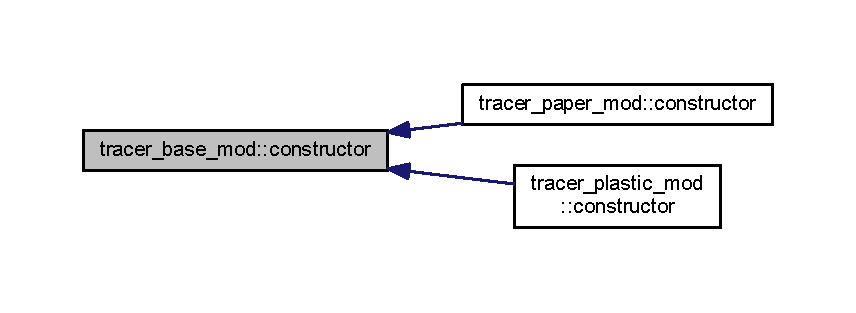
\includegraphics[width=350pt]{namespacetracer__base__mod_ab1e40296d34ae434e792768d1b77859f_icgraph}
\end{center}
\end{figure}
\mbox{\Hypertarget{namespacetracer__base__mod_a947559c248d9ddb1337721b71448167b}\label{namespacetracer__base__mod_a947559c248d9ddb1337721b71448167b}} 
\index{tracer\+\_\+base\+\_\+mod@{tracer\+\_\+base\+\_\+mod}!printtracer@{printtracer}}
\index{printtracer@{printtracer}!tracer\+\_\+base\+\_\+mod@{tracer\+\_\+base\+\_\+mod}}
\subsubsection{\texorpdfstring{printtracer()}{printtracer()}}
{\footnotesize\ttfamily subroutine tracer\+\_\+base\+\_\+mod\+::printtracer (\begin{DoxyParamCaption}\item[{class(\mbox{\hyperlink{structtracer__base__mod_1_1tracer__class}{tracer\+\_\+class}}), intent(inout)}]{self }\end{DoxyParamCaption})\hspace{0.3cm}{\ttfamily [private]}}



Method to print basic info about the Tracer. 

\begin{DoxyAuthor}{Author}
Ricardo Birjukovs Canelas -\/ M\+A\+R\+E\+T\+EC 
\end{DoxyAuthor}

\begin{DoxyParams}[1]{Parameters}
\mbox{\tt in}  & {\em self} & \\
\hline
\end{DoxyParams}


Definition at line 83 of file tracer\+\_\+base.\+f90.


\begin{DoxyCode}
83     \textcolor{keywordtype}{implicit none}
84     \textcolor{keywordtype}{class}(tracer\_class), \textcolor{keywordtype}{intent(inout)} :: self
85     \textcolor{keywordtype}{type}(string) :: outext, t(6)
86     \textcolor{keywordflow}{if} (self%now%active .eqv. .false.) \textcolor{keywordflow}{then}
87         outext = \textcolor{stringliteral}{'-->Tracer is inactive'}
88         \textcolor{keyword}{call }log%put(outext,.false.)
89     \textcolor{keywordflow}{else}
90         t(1) = self%par%id
91         t(2) = self%now%pos%x
92         t(3) = self%now%pos%y
93         t(4) = self%now%pos%z
94         outext = \textcolor{stringliteral}{'Tracer['}//t(1)//\textcolor{stringliteral}{']::xyz('}//t(2)//\textcolor{stringliteral}{','}//t(3)//\textcolor{stringliteral}{','}//t(4)//\textcolor{stringliteral}{')'}
95         \textcolor{keyword}{call }log%put(outext,.false.)
96 \textcolor{keywordflow}{    end if}
\end{DoxyCode}


\subsection{Variable Documentation}
\mbox{\Hypertarget{namespacetracer__base__mod_a6e04d44b4ef46cf27fb0e38290a98c14}\label{namespacetracer__base__mod_a6e04d44b4ef46cf27fb0e38290a98c14}} 
\index{tracer\+\_\+base\+\_\+mod@{tracer\+\_\+base\+\_\+mod}!dummytracer@{dummytracer}}
\index{dummytracer@{dummytracer}!tracer\+\_\+base\+\_\+mod@{tracer\+\_\+base\+\_\+mod}}
\subsubsection{\texorpdfstring{dummytracer}{dummytracer}}
{\footnotesize\ttfamily type(\mbox{\hyperlink{structtracer__base__mod_1_1tracer__class}{tracer\+\_\+class}}), public tracer\+\_\+base\+\_\+mod\+::dummytracer}



Just a template to allocate the generic arrays to this size. 



Definition at line 62 of file tracer\+\_\+base.\+f90.


\begin{DoxyCode}
62     \textcolor{keywordtype}{type}(tracer\_class) :: dummyTracer
\end{DoxyCode}

\hypertarget{namespacetracer__list__mod}{}\section{tracer\+\_\+list\+\_\+mod Module Reference}
\label{namespacetracer__list__mod}\index{tracer\+\_\+list\+\_\+mod@{tracer\+\_\+list\+\_\+mod}}


Module to hold the tracer linked list class and its methods. This class defines a double linked list to store any variable type, but with specific methods with type guards for Tracer objects. The class allows for insertion, deletion and iteration of the desired contents.  


\subsection*{Data Types}
\begin{DoxyCompactItemize}
\item 
type \mbox{\hyperlink{structtracer__list__mod_1_1tracerlist__class}{tracerlist\+\_\+class}}
\end{DoxyCompactItemize}
\subsection*{Functions/\+Subroutines}
\begin{DoxyCompactItemize}
\item 
subroutine \mbox{\hyperlink{namespacetracer__list__mod_a53919fa88a10347294eb6f2fccf072c7}{print\+\_\+tracerlist}} (this)
\begin{DoxyCompactList}\small\item\em Method that prints all the links of the list. \end{DoxyCompactList}\item 
subroutine \mbox{\hyperlink{namespacetracer__list__mod_a8c123eab5e919438e71cfc0b3847d384}{print\+\_\+tracerlistcurrent}} (this)
\begin{DoxyCompactList}\small\item\em Method that prints the current link of the list. \end{DoxyCompactList}\end{DoxyCompactItemize}


\subsection{Detailed Description}
Module to hold the tracer linked list class and its methods. This class defines a double linked list to store any variable type, but with specific methods with type guards for Tracer objects. The class allows for insertion, deletion and iteration of the desired contents. 

\begin{DoxyAuthor}{Author}
Ricardo Birjukovs Canelas 
\end{DoxyAuthor}


\subsection{Function/\+Subroutine Documentation}
\mbox{\Hypertarget{namespacetracer__list__mod_a53919fa88a10347294eb6f2fccf072c7}\label{namespacetracer__list__mod_a53919fa88a10347294eb6f2fccf072c7}} 
\index{tracer\+\_\+list\+\_\+mod@{tracer\+\_\+list\+\_\+mod}!print\+\_\+tracerlist@{print\+\_\+tracerlist}}
\index{print\+\_\+tracerlist@{print\+\_\+tracerlist}!tracer\+\_\+list\+\_\+mod@{tracer\+\_\+list\+\_\+mod}}
\subsubsection{\texorpdfstring{print\+\_\+tracerlist()}{print\_tracerlist()}}
{\footnotesize\ttfamily subroutine tracer\+\_\+list\+\_\+mod\+::print\+\_\+tracerlist (\begin{DoxyParamCaption}\item[{class(\mbox{\hyperlink{structtracer__list__mod_1_1tracerlist__class}{tracerlist\+\_\+class}}), intent(in)}]{this }\end{DoxyParamCaption})\hspace{0.3cm}{\ttfamily [private]}}



Method that prints all the links of the list. 

\begin{DoxyAuthor}{Author}
Ricardo Birjukovs Canelas -\/ M\+A\+R\+E\+T\+EC 
\end{DoxyAuthor}


Definition at line 47 of file tracer\+\_\+list.\+f90.


\begin{DoxyCode}
47     \textcolor{keywordtype}{class}(tracerList\_class), \textcolor{keywordtype}{intent(in)} :: this
48     \textcolor{keywordtype}{class}(*), \textcolor{keywordtype}{pointer} :: curr
49     \textcolor{keyword}{call }this%reset()               \textcolor{comment}{! reset list iterator}
50     \textcolor{keywordflow}{do} \textcolor{keywordflow}{while}(this%moreValues())     \textcolor{comment}{! loop while there are values to print}
51         \textcolor{keyword}{call }this%printCurrent()
52         \textcolor{keyword}{call }this%next()            \textcolor{comment}{! increment the list iterator}
53 \textcolor{keywordflow}{    end do}
54     \textcolor{keyword}{call }this%reset()               \textcolor{comment}{! reset list iterator}
\end{DoxyCode}
\mbox{\Hypertarget{namespacetracer__list__mod_a8c123eab5e919438e71cfc0b3847d384}\label{namespacetracer__list__mod_a8c123eab5e919438e71cfc0b3847d384}} 
\index{tracer\+\_\+list\+\_\+mod@{tracer\+\_\+list\+\_\+mod}!print\+\_\+tracerlistcurrent@{print\+\_\+tracerlistcurrent}}
\index{print\+\_\+tracerlistcurrent@{print\+\_\+tracerlistcurrent}!tracer\+\_\+list\+\_\+mod@{tracer\+\_\+list\+\_\+mod}}
\subsubsection{\texorpdfstring{print\+\_\+tracerlistcurrent()}{print\_tracerlistcurrent()}}
{\footnotesize\ttfamily subroutine tracer\+\_\+list\+\_\+mod\+::print\+\_\+tracerlistcurrent (\begin{DoxyParamCaption}\item[{class(\mbox{\hyperlink{structtracer__list__mod_1_1tracerlist__class}{tracerlist\+\_\+class}}), intent(in)}]{this }\end{DoxyParamCaption})\hspace{0.3cm}{\ttfamily [private]}}



Method that prints the current link of the list. 

\begin{DoxyAuthor}{Author}
Ricardo Birjukovs Canelas -\/ M\+A\+R\+E\+T\+EC 
\end{DoxyAuthor}


Definition at line 63 of file tracer\+\_\+list.\+f90.


\begin{DoxyCode}
63     \textcolor{keywordtype}{class}(tracerList\_class), \textcolor{keywordtype}{intent(in)} :: this
64     \textcolor{keywordtype}{class}(*), \textcolor{keywordtype}{pointer} :: curr
65     \textcolor{keywordtype}{type}(string) :: outext
66     curr => this%currentValue() \textcolor{comment}{! get current value}
67     \textcolor{keywordflow}{select type}(curr)
68 \textcolor{keywordflow}{    class is} (tracer\_class)
69         \textcolor{keyword}{call }curr%print()
70 \textcolor{keywordflow}{        class default}
71         outext = \textcolor{stringliteral}{'[tracerList\_class::print] Unexepected type of content, not a Tracer'}
72         \textcolor{keyword}{call }log%put(outext)
73         stop
74 \textcolor{keywordflow}{    end select}
\end{DoxyCode}

\hypertarget{namespacetracer__paper__mod}{}\section{tracer\+\_\+paper\+\_\+mod Module Reference}
\label{namespacetracer__paper__mod}\index{tracer\+\_\+paper\+\_\+mod@{tracer\+\_\+paper\+\_\+mod}}


Module that defines a Lagrangian tracer class for paper modelling and related methods. The type is defined as a derived type from the pule Lagrangian tracer, and hence inherits all of it\textquotesingle{}s data and methods.  


\subsection*{Data Types}
\begin{DoxyCompactItemize}
\item 
type \mbox{\hyperlink{structtracer__paper__mod_1_1paper__class}{paper\+\_\+class}}
\begin{DoxyCompactList}\small\item\em Type -\/ The plastic material Lagrangian tracer class. \end{DoxyCompactList}\item 
type \mbox{\hyperlink{structtracer__paper__mod_1_1paper__par__class}{paper\+\_\+par\+\_\+class}}
\item 
type \mbox{\hyperlink{structtracer__paper__mod_1_1paper__state__class}{paper\+\_\+state\+\_\+class}}
\begin{DoxyCompactList}\small\item\em Type -\/ State variables of a tracer object representing a paper material. \end{DoxyCompactList}\item 
interface \mbox{\hyperlink{interfacetracer__paper__mod_1_1papertracer}{papertracer}}
\end{DoxyCompactItemize}
\subsection*{Functions/\+Subroutines}
\begin{DoxyCompactItemize}
\item 
type(\mbox{\hyperlink{structtracer__paper__mod_1_1paper__class}{paper\+\_\+class}}) function \mbox{\hyperlink{namespacetracer__paper__mod_ab53f84300a313c395a5c3535f17022bb}{constructor}} (id, src, time, p)
\begin{DoxyCompactList}\small\item\em Paper Tracer constructor. \end{DoxyCompactList}\end{DoxyCompactItemize}


\subsection{Detailed Description}
Module that defines a Lagrangian tracer class for paper modelling and related methods. The type is defined as a derived type from the pule Lagrangian tracer, and hence inherits all of it\textquotesingle{}s data and methods. 

\begin{DoxyAuthor}{Author}
Ricardo Birjukovs Canelas 
\end{DoxyAuthor}


\subsection{Function/\+Subroutine Documentation}
\mbox{\Hypertarget{namespacetracer__paper__mod_ab53f84300a313c395a5c3535f17022bb}\label{namespacetracer__paper__mod_ab53f84300a313c395a5c3535f17022bb}} 
\index{tracer\+\_\+paper\+\_\+mod@{tracer\+\_\+paper\+\_\+mod}!constructor@{constructor}}
\index{constructor@{constructor}!tracer\+\_\+paper\+\_\+mod@{tracer\+\_\+paper\+\_\+mod}}
\subsubsection{\texorpdfstring{constructor()}{constructor()}}
{\footnotesize\ttfamily type(\mbox{\hyperlink{structtracer__paper__mod_1_1paper__class}{paper\+\_\+class}}) function tracer\+\_\+paper\+\_\+mod\+::constructor (\begin{DoxyParamCaption}\item[{integer, intent(in)}]{id,  }\item[{class(\mbox{\hyperlink{structsources__mod_1_1source__class}{source\+\_\+class}}), intent(in)}]{src,  }\item[{real(prec\+\_\+time), intent(in)}]{time,  }\item[{integer, intent(in)}]{p }\end{DoxyParamCaption})\hspace{0.3cm}{\ttfamily [private]}}



Paper Tracer constructor. 

\begin{DoxyAuthor}{Author}
Ricardo Birjukovs Canelas -\/ M\+A\+R\+E\+T\+EC 
\end{DoxyAuthor}

\begin{DoxyParams}[1]{Parameters}
\mbox{\tt in}  & {\em id,src,time,p} & \\
\hline
\end{DoxyParams}


Definition at line 69 of file tracer\+\_\+paper.\+f90.


\begin{DoxyCode}
69         \textcolor{keywordtype}{implicit none}
70         \textcolor{keywordtype}{type}(paper\_class) :: constructor
71         \textcolor{keywordtype}{integer}, \textcolor{keywordtype}{intent(in)} :: id
72         \textcolor{keywordtype}{class}(source\_class), \textcolor{keywordtype}{intent(in)} :: src
73         \textcolor{keywordtype}{real(prec\_time)}, \textcolor{keywordtype}{intent(in)} :: time
74         \textcolor{keywordtype}{integer}, \textcolor{keywordtype}{intent(in)} :: p
75         \textcolor{keywordtype}{class}(*), \textcolor{keywordtype}{allocatable} :: base\_trc
76 
77         \textcolor{comment}{!use the base class constructor to build the base of our new derived type}
78         constructor%tracer\_class = tracer(id,src,time,p)
79         \textcolor{comment}{!VERY NICE IFORT BUG (I think) - only some of the variables get used using the base constructor... }
80         constructor%par%id = id \textcolor{comment}{!forcing}
81         constructor%par%idsource = src%par%id \textcolor{comment}{!forcing }
82         \textcolor{comment}{!now initialize the specific components of this derived type}
83         \textcolor{comment}{!material parameters}
84         constructor%mpar%degradation\_rate = src%prop%degrd\_rate
85         constructor%mpar%particulate = src%prop%particulate
86         constructor%mpar%size = src%prop%radius
87         \textcolor{comment}{!material state}
88         constructor%mnow%density = src%prop%density
89         constructor%mnow%condition = src%prop%condition
90         constructor%mnow%radius = src%prop%radius
91         constructor%mnow%concentration = mv
92         \textcolor{keywordflow}{if} (constructor%mpar%particulate) \textcolor{keywordflow}{then}
93             constructor%mpar%size = src%prop%pt\_radius \textcolor{comment}{!correcting size to now mean particle size, not
       tracer size}
94             constructor%mnow%concentration = src%prop%ini\_concentration
95 \textcolor{keywordflow}{        end if}
96     
\end{DoxyCode}
Here is the call graph for this function\+:
\nopagebreak
\begin{figure}[H]
\begin{center}
\leavevmode
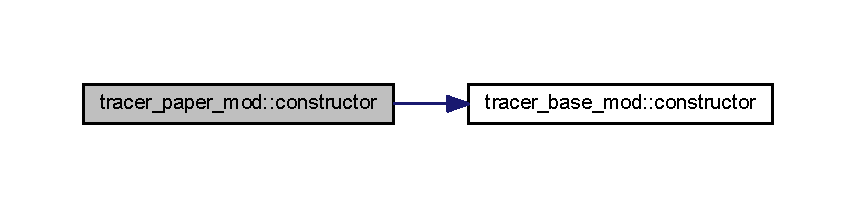
\includegraphics[width=350pt]{namespacetracer__paper__mod_ab53f84300a313c395a5c3535f17022bb_cgraph}
\end{center}
\end{figure}

\hypertarget{namespacetracer__plastic__mod}{}\section{tracer\+\_\+plastic\+\_\+mod Module Reference}
\label{namespacetracer__plastic__mod}\index{tracer\+\_\+plastic\+\_\+mod@{tracer\+\_\+plastic\+\_\+mod}}


Module that defines a Lagrangian tracer class for plastic modelling and related methods. The type is defined as a derived type from the pule Lagrangian tracer, and hence inherits all of it\textquotesingle{}s data and methods.  


\subsection*{Data Types}
\begin{DoxyCompactItemize}
\item 
type \mbox{\hyperlink{structtracer__plastic__mod_1_1plastic__class}{plastic\+\_\+class}}
\begin{DoxyCompactList}\small\item\em Type -\/ The plastic material Lagrangian tracer class. \end{DoxyCompactList}\item 
type \mbox{\hyperlink{structtracer__plastic__mod_1_1plastic__par__class}{plastic\+\_\+par\+\_\+class}}
\item 
type \mbox{\hyperlink{structtracer__plastic__mod_1_1plastic__state__class}{plastic\+\_\+state\+\_\+class}}
\begin{DoxyCompactList}\small\item\em Type -\/ State variables of a tracer object representing a plastic material. \end{DoxyCompactList}\end{DoxyCompactItemize}
\subsection*{Functions/\+Subroutines}
\begin{DoxyCompactItemize}
\item 
subroutine \mbox{\hyperlink{namespacetracer__plastic__mod_a42882cd86cfe30f341d8150582a664a9}{plastic\+\_\+initialize}} (trc, id, id\+\_\+source, time, pt)
\begin{DoxyCompactList}\small\item\em Tracer initialization method. \end{DoxyCompactList}\end{DoxyCompactItemize}


\subsection{Detailed Description}
Module that defines a Lagrangian tracer class for plastic modelling and related methods. The type is defined as a derived type from the pule Lagrangian tracer, and hence inherits all of it\textquotesingle{}s data and methods. 

\begin{DoxyAuthor}{Author}
Ricardo Birjukovs Canelas 
\end{DoxyAuthor}


\subsection{Function/\+Subroutine Documentation}
\mbox{\Hypertarget{namespacetracer__plastic__mod_a42882cd86cfe30f341d8150582a664a9}\label{namespacetracer__plastic__mod_a42882cd86cfe30f341d8150582a664a9}} 
\index{tracer\+\_\+plastic\+\_\+mod@{tracer\+\_\+plastic\+\_\+mod}!plastic\+\_\+initialize@{plastic\+\_\+initialize}}
\index{plastic\+\_\+initialize@{plastic\+\_\+initialize}!tracer\+\_\+plastic\+\_\+mod@{tracer\+\_\+plastic\+\_\+mod}}
\subsubsection{\texorpdfstring{plastic\+\_\+initialize()}{plastic\_initialize()}}
{\footnotesize\ttfamily subroutine tracer\+\_\+plastic\+\_\+mod\+::plastic\+\_\+initialize (\begin{DoxyParamCaption}\item[{class(\mbox{\hyperlink{structtracer__plastic__mod_1_1plastic__class}{plastic\+\_\+class}})}]{trc,  }\item[{integer, intent(in)}]{id,  }\item[{integer, intent(in)}]{id\+\_\+source,  }\item[{real(prec\+\_\+time), intent(in)}]{time,  }\item[{type(vector), intent(in)}]{pt }\end{DoxyParamCaption})\hspace{0.3cm}{\ttfamily [private]}}



Tracer initialization method. 

\begin{DoxyAuthor}{Author}
Ricardo Birjukovs Canelas -\/ M\+A\+R\+E\+T\+EC 
\end{DoxyAuthor}

\begin{DoxyParams}[1]{Parameters}
\mbox{\tt in}  & {\em trc,id,id\+\_\+source,time,pt} & \\
\hline
\end{DoxyParams}


Definition at line 61 of file tracer\+\_\+plastic.\+f90.


\begin{DoxyCode}
61     \textcolor{keywordtype}{implicit none}
62     \textcolor{keywordtype}{class}(plastic\_class) :: trc
63     \textcolor{keywordtype}{integer}, \textcolor{keywordtype}{intent(in)} :: id
64     \textcolor{keywordtype}{integer}, \textcolor{keywordtype}{intent(in)} :: id\_source
65     \textcolor{keywordtype}{type}(vector), \textcolor{keywordtype}{intent(in)} :: pt
66     \textcolor{keywordtype}{real(prec\_time)}, \textcolor{keywordtype}{intent(in)} :: time
67 
68     \textcolor{comment}{! initialize parameters}
69     trc%par%id = id
70     trc%par%idsource = id\_source
71     trc%par%velmax = 15.0 \textcolor{comment}{!(m/s, just a placeholder)}
72     \textcolor{comment}{! initialize tracer state}
73     trc%now%age=0.0
74     trc%now%active = .false.
75     trc%now%pos = pt
76     trc%now%vel = 0.0
77     trc%now%acc = 0.0
78     trc%now%depth = 0.0
79     \textcolor{comment}{! Initialize statistical accumulator variables}
80     trc%stats%acc\_pos = 0.0
81     trc%stats%acc\_vel = 0.0
82     trc%stats%acc\_depth = 0.0
83     trc%stats%ns = 0
84 
\end{DoxyCode}

\hypertarget{namespacetracers__mod}{}\section{tracers\+\_\+mod Module Reference}
\label{namespacetracers__mod}\index{tracers\+\_\+mod@{tracers\+\_\+mod}}


Module to hold and \textquotesingle{}wrap\textquotesingle{} all the tracer respective modules.  




\subsection{Detailed Description}
Module to hold and \textquotesingle{}wrap\textquotesingle{} all the tracer respective modules. 

\begin{DoxyAuthor}{Author}
Ricardo Birjukovs Canelas 
\end{DoxyAuthor}

\hypertarget{namespaceutilities__mod}{}\section{utilities\+\_\+mod Module Reference}
\label{namespaceutilities__mod}\index{utilities\+\_\+mod@{utilities\+\_\+mod}}


Module that provides useful back-\/end routines.  


\subsection*{Data Types}
\begin{DoxyCompactItemize}
\item 
type \mbox{\hyperlink{structutilities__mod_1_1utils__class}{utils\+\_\+class}}
\end{DoxyCompactItemize}
\subsection*{Functions/\+Subroutines}
\begin{DoxyCompactItemize}
\item 
integer function, dimension(6) \mbox{\hyperlink{namespaceutilities__mod_ab5b97f243f9347a40db76d55509d37ca}{getdatefromisostring}} (self, date\+Str)
\begin{DoxyCompactList}\small\item\em Function that returns an integer array of type (year, month, day, hour, minute, second) from an I\+SO date string. \end{DoxyCompactList}\item 
integer function \mbox{\hyperlink{namespaceutilities__mod_ad446cce78a6509db0e839439a0e84564}{find\+\_\+str}} (self, str\+\_\+array, str, mandatory)
\begin{DoxyCompactList}\small\item\em returns the index of a given string in an array of strings. Has optional mandatory flag. \end{DoxyCompactList}\item 
type(vector) function \mbox{\hyperlink{namespaceutilities__mod_ad6e463f7e5fc49fe4fcd5464326ade01}{geo2m}} (self, geovec, lat)
\begin{DoxyCompactList}\small\item\em Returns a vector in meters given an array in geographical coordinates (lon, lat, z) and a lattitude. \end{DoxyCompactList}\item 
type(vector) function \mbox{\hyperlink{namespaceutilities__mod_a70b21b18c8633b7fd4c3057530d3f16f}{m2geo\+\_\+vec}} (self, mvec, lat)
\begin{DoxyCompactList}\small\item\em Returns a vector in geographical coordinates (lon, lat, z) given an array in meters and a lattitude. \end{DoxyCompactList}\item 
real(prec) function, dimension(size(mvec)) \mbox{\hyperlink{namespaceutilities__mod_ae6b8a45b229e3f1f8c2b12dd74e7a2dd}{m2geo\+\_\+comp}} (self, mvec, lat, component)
\begin{DoxyCompactList}\small\item\em Returns a vector in geographical coordinates (lon, lat, z) given an array in meters and a lattitude. \end{DoxyCompactList}\item 
character(\+:) function, allocatable \mbox{\hyperlink{namespaceutilities__mod_a6ba00b0a503f26c7e755d1efbbe83c5b}{int2str}} (self, fmt, i)
\begin{DoxyCompactList}\small\item\em Returns a zero paded string from an integer number and a format descriptor. \end{DoxyCompactList}\item 
real(prec) function \mbox{\hyperlink{namespaceutilities__mod_a164054d89c012d95f63c12a6cc0ac8d7}{get\+\_\+closest\+\_\+twopow}} (self, num)
\begin{DoxyCompactList}\small\item\em Returns the closest power of 2 or a given real number. \end{DoxyCompactList}\end{DoxyCompactItemize}
\subsection*{Variables}
\begin{DoxyCompactItemize}
\item 
type(\mbox{\hyperlink{structutilities__mod_1_1utils__class}{utils\+\_\+class}}), public \mbox{\hyperlink{namespaceutilities__mod_aa12c2506b3107528a2511d059186f12d}{utils}}
\end{DoxyCompactItemize}


\subsection{Detailed Description}
Module that provides useful back-\/end routines. 

\begin{DoxyAuthor}{Author}
Ricardo Birjukovs Canelas 
\end{DoxyAuthor}


\subsection{Function/\+Subroutine Documentation}
\mbox{\Hypertarget{namespaceutilities__mod_ad446cce78a6509db0e839439a0e84564}\label{namespaceutilities__mod_ad446cce78a6509db0e839439a0e84564}} 
\index{utilities\+\_\+mod@{utilities\+\_\+mod}!find\+\_\+str@{find\+\_\+str}}
\index{find\+\_\+str@{find\+\_\+str}!utilities\+\_\+mod@{utilities\+\_\+mod}}
\subsubsection{\texorpdfstring{find\+\_\+str()}{find\_str()}}
{\footnotesize\ttfamily integer function utilities\+\_\+mod\+::find\+\_\+str (\begin{DoxyParamCaption}\item[{class(\mbox{\hyperlink{structutilities__mod_1_1utils__class}{utils\+\_\+class}}), intent(in)}]{self,  }\item[{type(string), dimension(\+:), intent(in)}]{str\+\_\+array,  }\item[{type(string), intent(in)}]{str,  }\item[{logical, intent(in), optional}]{mandatory }\end{DoxyParamCaption})\hspace{0.3cm}{\ttfamily [private]}}



returns the index of a given string in an array of strings. Has optional mandatory flag. 

\begin{DoxyAuthor}{Author}
Ricardo Birjukovs Canelas -\/ M\+A\+R\+E\+T\+EC 
\end{DoxyAuthor}

\begin{DoxyParams}[1]{Parameters}
\mbox{\tt in}  & {\em self,str\+\_\+array,str,mandatory} & \\
\hline
\end{DoxyParams}


Definition at line 82 of file utilities.\+f90.


\begin{DoxyCode}
82     \textcolor{keywordtype}{class}(utils\_class), \textcolor{keywordtype}{intent(in)} :: self
83     \textcolor{keywordtype}{type}(string), \textcolor{keywordtype}{dimension(:)}, \textcolor{keywordtype}{intent(in)} :: str\_array
84     \textcolor{keywordtype}{type}(string), \textcolor{keywordtype}{intent(in)} :: str
85     \textcolor{keywordtype}{logical}, \textcolor{keywordtype}{optional}, \textcolor{keywordtype}{intent(in)} :: mandatory
86     \textcolor{keywordtype}{type}(string) :: outext
87     \textcolor{keywordflow}{do} find\_str=1, \textcolor{keyword}{size}(str\_array)
88         \textcolor{keywordflow}{if} (str == str\_array(find\_str)) \textcolor{keywordflow}{return}
89 \textcolor{keywordflow}{    end do}
90     \textcolor{keywordflow}{if}(\textcolor{keyword}{present}(mandatory)) \textcolor{keywordflow}{then}
91         \textcolor{keywordflow}{if} (mandatory) \textcolor{keywordflow}{then}
92             outext = \textcolor{stringliteral}{'[Utils::find\_str]: string "'}// str //\textcolor{stringliteral}{'" not found on list, stopping'}
93             \textcolor{keyword}{call }log%put(outext)
94             stop
95 \textcolor{keywordflow}{        end if}
96 \textcolor{keywordflow}{    end if}
\end{DoxyCode}
\mbox{\Hypertarget{namespaceutilities__mod_ad6e463f7e5fc49fe4fcd5464326ade01}\label{namespaceutilities__mod_ad6e463f7e5fc49fe4fcd5464326ade01}} 
\index{utilities\+\_\+mod@{utilities\+\_\+mod}!geo2m@{geo2m}}
\index{geo2m@{geo2m}!utilities\+\_\+mod@{utilities\+\_\+mod}}
\subsubsection{\texorpdfstring{geo2m()}{geo2m()}}
{\footnotesize\ttfamily type(vector) function utilities\+\_\+mod\+::geo2m (\begin{DoxyParamCaption}\item[{class(\mbox{\hyperlink{structutilities__mod_1_1utils__class}{utils\+\_\+class}}), intent(in)}]{self,  }\item[{type(vector), intent(in)}]{geovec,  }\item[{real(prec), intent(in)}]{lat }\end{DoxyParamCaption})\hspace{0.3cm}{\ttfamily [private]}}



Returns a vector in meters given an array in geographical coordinates (lon, lat, z) and a lattitude. 

\begin{DoxyAuthor}{Author}
Ricardo Birjukovs Canelas -\/ M\+A\+R\+E\+T\+EC 
\end{DoxyAuthor}

\begin{DoxyParams}[1]{Parameters}
\mbox{\tt in}  & {\em self,geovec,lat} & \\
\hline
\end{DoxyParams}


Definition at line 107 of file utilities.\+f90.


\begin{DoxyCode}
107     \textcolor{keywordtype}{class}(utils\_class), \textcolor{keywordtype}{intent(in)} :: self
108     \textcolor{keywordtype}{type}(vector), \textcolor{keywordtype}{intent(in)} :: geovec
109     \textcolor{keywordtype}{real(prec)}, \textcolor{keywordtype}{intent(in)} :: lat
110     \textcolor{keywordtype}{integer} :: R
111     \textcolor{keywordtype}{real(prec)} :: pi = 4*atan(1.0)
112     r = 6378137 \textcolor{comment}{!earth radius in meters}
113     \textcolor{comment}{!pi = 3.1415926}
114     res = geovec
115     res%x = res%x*r*cos(pi*lat/180.0)
116     res%y = res%y*r
\end{DoxyCode}
\mbox{\Hypertarget{namespaceutilities__mod_a164054d89c012d95f63c12a6cc0ac8d7}\label{namespaceutilities__mod_a164054d89c012d95f63c12a6cc0ac8d7}} 
\index{utilities\+\_\+mod@{utilities\+\_\+mod}!get\+\_\+closest\+\_\+twopow@{get\+\_\+closest\+\_\+twopow}}
\index{get\+\_\+closest\+\_\+twopow@{get\+\_\+closest\+\_\+twopow}!utilities\+\_\+mod@{utilities\+\_\+mod}}
\subsubsection{\texorpdfstring{get\+\_\+closest\+\_\+twopow()}{get\_closest\_twopow()}}
{\footnotesize\ttfamily real(prec) function utilities\+\_\+mod\+::get\+\_\+closest\+\_\+twopow (\begin{DoxyParamCaption}\item[{class(\mbox{\hyperlink{structutilities__mod_1_1utils__class}{utils\+\_\+class}}), intent(in)}]{self,  }\item[{real(prec), intent(in)}]{num }\end{DoxyParamCaption})\hspace{0.3cm}{\ttfamily [private]}}



Returns the closest power of 2 or a given real number. 

\begin{DoxyAuthor}{Author}
Ricardo Birjukovs Canelas -\/ M\+A\+R\+E\+T\+EC 
\end{DoxyAuthor}

\begin{DoxyParams}[1]{Parameters}
\mbox{\tt in}  & {\em self,num} & \\
\hline
\end{DoxyParams}


Definition at line 187 of file utilities.\+f90.


\begin{DoxyCode}
187     \textcolor{keywordtype}{class}(utils\_class), \textcolor{keywordtype}{intent(in)} :: self
188     \textcolor{keywordtype}{real(prec)}, \textcolor{keywordtype}{intent(in)} :: num
189     \textcolor{keywordtype}{real(prec)} :: twopow
190     \textcolor{keywordtype}{integer} :: i
191     \textcolor{keywordtype}{real(prec)} :: dist1, dist2
192     \textcolor{keywordflow}{do} i=-4, 10
193         twopow = 2.0**i
194         \textcolor{keywordflow}{if} (num < twopow) \textcolor{keywordflow}{then}
195             dist1 = sqrt(twopow-num)
196             dist2 = sqrt(num-2.0**(i-1))
197             \textcolor{keywordflow}{if} (dist2 < dist1) \textcolor{keywordflow}{then}
198                 twopow = 2.0**(i-1)
199                 \textcolor{keywordflow}{exit}
200 \textcolor{keywordflow}{            endif}
201             \textcolor{keywordflow}{exit}
202 \textcolor{keywordflow}{        endif}
203 \textcolor{keywordflow}{    enddo}
\end{DoxyCode}
\mbox{\Hypertarget{namespaceutilities__mod_ab5b97f243f9347a40db76d55509d37ca}\label{namespaceutilities__mod_ab5b97f243f9347a40db76d55509d37ca}} 
\index{utilities\+\_\+mod@{utilities\+\_\+mod}!getdatefromisostring@{getdatefromisostring}}
\index{getdatefromisostring@{getdatefromisostring}!utilities\+\_\+mod@{utilities\+\_\+mod}}
\subsubsection{\texorpdfstring{getdatefromisostring()}{getdatefromisostring()}}
{\footnotesize\ttfamily integer function, dimension(6) utilities\+\_\+mod\+::getdatefromisostring (\begin{DoxyParamCaption}\item[{class(\mbox{\hyperlink{structutilities__mod_1_1utils__class}{utils\+\_\+class}}), intent(in)}]{self,  }\item[{type(string), intent(in)}]{date\+Str }\end{DoxyParamCaption})\hspace{0.3cm}{\ttfamily [private]}}



Function that returns an integer array of type (year, month, day, hour, minute, second) from an I\+SO date string. 

\begin{DoxyAuthor}{Author}
Ricardo Birjukovs Canelas -\/ M\+A\+R\+E\+T\+EC 
\end{DoxyAuthor}

\begin{DoxyParams}[1]{Parameters}
\mbox{\tt in}  & {\em self,date\+Str} & \\
\hline
\end{DoxyParams}


Definition at line 56 of file utilities.\+f90.


\begin{DoxyCode}
56     \textcolor{keywordtype}{class}(utils\_class), \textcolor{keywordtype}{intent(in)} :: self
57     \textcolor{keywordtype}{type}(string), \textcolor{keywordtype}{intent(in)} :: dateStr
58     \textcolor{keywordtype}{integer}, \textcolor{keywordtype}{dimension(6)} :: getDateFromISOString
59     \textcolor{keywordtype}{integer} :: i
60     \textcolor{keywordtype}{type}(string), \textcolor{keywordtype}{allocatable} :: dc(:)
61     \textcolor{keywordtype}{type}(string) :: outext
62     \textcolor{keyword}{call }datestr%split(tokens=dc, sep=\textcolor{stringliteral}{' '})
63     \textcolor{keywordflow}{if} (\textcolor{keyword}{size}(dc) == 6) \textcolor{keywordflow}{then}
64         \textcolor{keywordflow}{do} i=1, \textcolor{keyword}{size}(dc)
65             getdatefromisostring(i) = dc(i)%to\_number(kind=1.\_r4p)
66 \textcolor{keywordflow}{        end do}
67     \textcolor{keywordflow}{else}
68         outext = \textcolor{stringliteral}{'[Utils::getDateFromISOString] Date '}// datestr //\textcolor{stringliteral}{' not in correct format. Eg. "2009 3 1 0
       0 0"'}
69         \textcolor{keyword}{call }log%put(outext)
70         stop
71 \textcolor{keywordflow}{    end if}    
\end{DoxyCode}
\mbox{\Hypertarget{namespaceutilities__mod_a6ba00b0a503f26c7e755d1efbbe83c5b}\label{namespaceutilities__mod_a6ba00b0a503f26c7e755d1efbbe83c5b}} 
\index{utilities\+\_\+mod@{utilities\+\_\+mod}!int2str@{int2str}}
\index{int2str@{int2str}!utilities\+\_\+mod@{utilities\+\_\+mod}}
\subsubsection{\texorpdfstring{int2str()}{int2str()}}
{\footnotesize\ttfamily character(\+:) function, allocatable utilities\+\_\+mod\+::int2str (\begin{DoxyParamCaption}\item[{class(\mbox{\hyperlink{structutilities__mod_1_1utils__class}{utils\+\_\+class}}), intent(in)}]{self,  }\item[{character(len=6), intent(in)}]{fmt,  }\item[{integer, intent(in)}]{i }\end{DoxyParamCaption})\hspace{0.3cm}{\ttfamily [private]}}



Returns a zero paded string from an integer number and a format descriptor. 

\begin{DoxyAuthor}{Author}
Ricardo Birjukovs Canelas -\/ M\+A\+R\+E\+T\+EC 
\end{DoxyAuthor}

\begin{DoxyParams}[1]{Parameters}
\mbox{\tt in}  & {\em self,fmt,i} & \\
\hline
\end{DoxyParams}


Definition at line 171 of file utilities.\+f90.


\begin{DoxyCode}
171     \textcolor{keywordtype}{class}(utils\_class), \textcolor{keywordtype}{intent(in)} :: self
172     \textcolor{keywordtype}{character(:)}, \textcolor{keywordtype}{allocatable} :: res
173     \textcolor{keywordtype}{character(len=6)}, \textcolor{keywordtype}{intent(in)} :: fmt \textcolor{comment}{! format descriptor}
174     \textcolor{keywordtype}{integer}, \textcolor{keywordtype}{intent(in)} :: i
175     \textcolor{keywordtype}{character(range(i)+2)} :: tmp
176     \textcolor{keyword}{write}(tmp, fmt) i
177     res = trim(tmp)
\end{DoxyCode}
\mbox{\Hypertarget{namespaceutilities__mod_ae6b8a45b229e3f1f8c2b12dd74e7a2dd}\label{namespaceutilities__mod_ae6b8a45b229e3f1f8c2b12dd74e7a2dd}} 
\index{utilities\+\_\+mod@{utilities\+\_\+mod}!m2geo\+\_\+comp@{m2geo\+\_\+comp}}
\index{m2geo\+\_\+comp@{m2geo\+\_\+comp}!utilities\+\_\+mod@{utilities\+\_\+mod}}
\subsubsection{\texorpdfstring{m2geo\+\_\+comp()}{m2geo\_comp()}}
{\footnotesize\ttfamily real(prec) function, dimension(size(mvec)) utilities\+\_\+mod\+::m2geo\+\_\+comp (\begin{DoxyParamCaption}\item[{class(\mbox{\hyperlink{structutilities__mod_1_1utils__class}{utils\+\_\+class}}), intent(in)}]{self,  }\item[{real(prec), dimension(\+:), intent(in)}]{mvec,  }\item[{real(prec), dimension(\+:), intent(in)}]{lat,  }\item[{logical, intent(in)}]{component }\end{DoxyParamCaption})\hspace{0.3cm}{\ttfamily [private]}}



Returns a vector in geographical coordinates (lon, lat, z) given an array in meters and a lattitude. 

\begin{DoxyAuthor}{Author}
Ricardo Birjukovs Canelas -\/ M\+A\+R\+E\+T\+EC 
\end{DoxyAuthor}

\begin{DoxyParams}[1]{Parameters}
\mbox{\tt in}  & {\em self,mvec,lat} & \\
\hline
\end{DoxyParams}


Definition at line 147 of file utilities.\+f90.


\begin{DoxyCode}
147     \textcolor{keywordtype}{class}(utils\_class), \textcolor{keywordtype}{intent(in)} :: self
148     \textcolor{keywordtype}{real(prec)}, \textcolor{keywordtype}{dimension(:)}, \textcolor{keywordtype}{intent(in)} :: mvec    
149     \textcolor{keywordtype}{real(prec)}, \textcolor{keywordtype}{dimension(:)}, \textcolor{keywordtype}{intent(in)} :: lat
150     \textcolor{keywordtype}{logical}, \textcolor{keywordtype}{intent(in)} :: component
151     \textcolor{keywordtype}{real(prec)}, \textcolor{keywordtype}{dimension(size(mvec))} :: m2geo\_comp
152     \textcolor{keywordtype}{real(prec)} :: R
153     \textcolor{keywordtype}{real(prec)} :: pi = 4*atan(1.0)
154     r = 6378137.0 \textcolor{comment}{!earth radius in meters}
155     m2geo\_comp = mvec
156     \textcolor{keywordflow}{if} (component) \textcolor{keywordflow}{then}
157         m2geo\_comp = m2geo\_comp/(r*pi/180.0)
158     \textcolor{keywordflow}{else}
159         m2geo\_comp = m2geo\_comp/((r*pi/180.0)*cos(pi*lat/180.0))
160 \textcolor{keywordflow}{    end if}
\end{DoxyCode}
Here is the caller graph for this function\+:\nopagebreak
\begin{figure}[H]
\begin{center}
\leavevmode
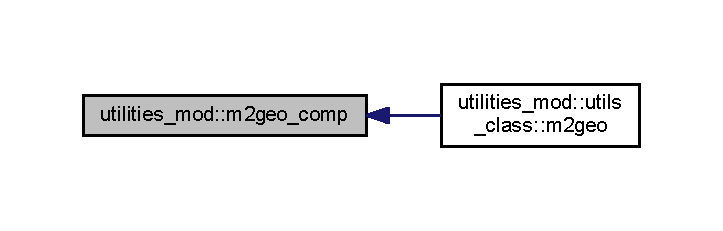
\includegraphics[width=347pt]{namespaceutilities__mod_ae6b8a45b229e3f1f8c2b12dd74e7a2dd_icgraph}
\end{center}
\end{figure}
\mbox{\Hypertarget{namespaceutilities__mod_a70b21b18c8633b7fd4c3057530d3f16f}\label{namespaceutilities__mod_a70b21b18c8633b7fd4c3057530d3f16f}} 
\index{utilities\+\_\+mod@{utilities\+\_\+mod}!m2geo\+\_\+vec@{m2geo\+\_\+vec}}
\index{m2geo\+\_\+vec@{m2geo\+\_\+vec}!utilities\+\_\+mod@{utilities\+\_\+mod}}
\subsubsection{\texorpdfstring{m2geo\+\_\+vec()}{m2geo\_vec()}}
{\footnotesize\ttfamily type(vector) function utilities\+\_\+mod\+::m2geo\+\_\+vec (\begin{DoxyParamCaption}\item[{class(\mbox{\hyperlink{structutilities__mod_1_1utils__class}{utils\+\_\+class}}), intent(in)}]{self,  }\item[{type(vector), intent(in)}]{mvec,  }\item[{real(prec), intent(in)}]{lat }\end{DoxyParamCaption})\hspace{0.3cm}{\ttfamily [private]}}



Returns a vector in geographical coordinates (lon, lat, z) given an array in meters and a lattitude. 

\begin{DoxyAuthor}{Author}
Ricardo Birjukovs Canelas -\/ M\+A\+R\+E\+T\+EC 
\end{DoxyAuthor}

\begin{DoxyParams}[1]{Parameters}
\mbox{\tt in}  & {\em self,mvec,lat} & \\
\hline
\end{DoxyParams}


Definition at line 127 of file utilities.\+f90.


\begin{DoxyCode}
127     \textcolor{keywordtype}{class}(utils\_class), \textcolor{keywordtype}{intent(in)} :: self
128     \textcolor{keywordtype}{type}(vector), \textcolor{keywordtype}{intent(in)} :: mvec    
129     \textcolor{keywordtype}{real(prec)}, \textcolor{keywordtype}{intent(in)} :: lat
130     \textcolor{keywordtype}{real(prec)} :: R
131     \textcolor{keywordtype}{real(prec)} :: pi = 4*atan(1.0)
132     r = 6378137.0 \textcolor{comment}{!earth radius in meters}
133     \textcolor{comment}{!pi = 3.1415926}
134     res = mvec
135     res%y = res%y/(r*pi/180.0)
136     res%x = res%x/((r*pi/180.0)*cos(pi*res%y/180.0))
\end{DoxyCode}
Here is the caller graph for this function\+:\nopagebreak
\begin{figure}[H]
\begin{center}
\leavevmode
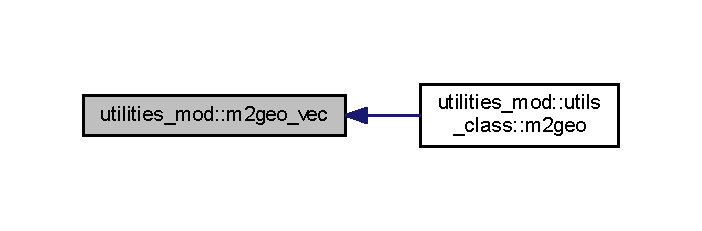
\includegraphics[width=337pt]{namespaceutilities__mod_a70b21b18c8633b7fd4c3057530d3f16f_icgraph}
\end{center}
\end{figure}


\subsection{Variable Documentation}
\mbox{\Hypertarget{namespaceutilities__mod_aa12c2506b3107528a2511d059186f12d}\label{namespaceutilities__mod_aa12c2506b3107528a2511d059186f12d}} 
\index{utilities\+\_\+mod@{utilities\+\_\+mod}!utils@{utils}}
\index{utils@{utils}!utilities\+\_\+mod@{utilities\+\_\+mod}}
\subsubsection{\texorpdfstring{utils}{utils}}
{\footnotesize\ttfamily type(\mbox{\hyperlink{structutilities__mod_1_1utils__class}{utils\+\_\+class}}), public utilities\+\_\+mod\+::utils}



Definition at line 41 of file utilities.\+f90.


\begin{DoxyCode}
41     \textcolor{keywordtype}{type}(utils\_class) :: Utils
\end{DoxyCode}

\hypertarget{namespacevtkwritter__mod}{}\section{vtkwritter\+\_\+mod Module Reference}
\label{namespacevtkwritter__mod}\index{vtkwritter\+\_\+mod@{vtkwritter\+\_\+mod}}


Defines a vtk writer class with an object exposable to the Output streamer. Writes files in .xml vtk, both in serial and parallel model. Uses an unstructured mesh format specifier to store any type of data, both meshes and Tracers. Supports scalar and vectorial data.  


\subsection*{Data Types}
\begin{DoxyCompactItemize}
\item 
type \mbox{\hyperlink{structvtkwritter__mod_1_1vtkwritter__class}{vtkwritter\+\_\+class}}
\end{DoxyCompactItemize}
\subsection*{Functions/\+Subroutines}
\begin{DoxyCompactItemize}
\item 
subroutine \mbox{\hyperlink{namespacevtkwritter__mod_abd35d591c8e15730a277b2d26deb83e8}{initvtkwritter}} (self)
\begin{DoxyCompactList}\small\item\em Initializes a V\+TK writer object. \end{DoxyCompactList}\item 
subroutine \mbox{\hyperlink{namespacevtkwritter__mod_ac11e4d1d71141e6de89ba67508212ce0}{tracerserial}} (self, filename, blocks)
\begin{DoxyCompactList}\small\item\em Public Tracer writting routine. Writes Tracer data in binary X\+ML V\+TK format using an unstructured grid. Serial writer for serial files. \end{DoxyCompactList}\item 
subroutine \mbox{\hyperlink{namespacevtkwritter__mod_a9f44d9fd1c5da759c4f2d721d12a8181}{domain}} (self, filename, bbox, npbbox, blocks)
\begin{DoxyCompactList}\small\item\em Public simulation domain writting routine. Writes binary X\+ML V\+TK format using an unstructured grid. \end{DoxyCompactList}\end{DoxyCompactItemize}
\subsection*{Variables}
\begin{DoxyCompactItemize}
\item 
type(\mbox{\hyperlink{structvtkwritter__mod_1_1vtkwritter__class}{vtkwritter\+\_\+class}}), public \mbox{\hyperlink{namespacevtkwritter__mod_a80eabc5e7153822e7ddd54b662294c81}{vtkwritter}}
\end{DoxyCompactItemize}


\subsection{Detailed Description}
Defines a vtk writer class with an object exposable to the Output streamer. Writes files in .xml vtk, both in serial and parallel model. Uses an unstructured mesh format specifier to store any type of data, both meshes and Tracers. Supports scalar and vectorial data. 

\begin{DoxyAuthor}{Author}
Ricardo Birjukovs Canelas 
\end{DoxyAuthor}


\subsection{Function/\+Subroutine Documentation}
\mbox{\Hypertarget{namespacevtkwritter__mod_a9f44d9fd1c5da759c4f2d721d12a8181}\label{namespacevtkwritter__mod_a9f44d9fd1c5da759c4f2d721d12a8181}} 
\index{vtkwritter\+\_\+mod@{vtkwritter\+\_\+mod}!domain@{domain}}
\index{domain@{domain}!vtkwritter\+\_\+mod@{vtkwritter\+\_\+mod}}
\subsubsection{\texorpdfstring{domain()}{domain()}}
{\footnotesize\ttfamily subroutine vtkwritter\+\_\+mod\+::domain (\begin{DoxyParamCaption}\item[{class(\mbox{\hyperlink{structvtkwritter__mod_1_1vtkwritter__class}{vtkwritter\+\_\+class}}), intent(inout)}]{self,  }\item[{type(string), intent(in)}]{filename,  }\item[{class(\mbox{\hyperlink{structboundingbox__mod_1_1boundingbox__class}{boundingbox\+\_\+class}}), intent(in)}]{bbox,  }\item[{integer, intent(in)}]{npbbox,  }\item[{class(\mbox{\hyperlink{structblocks__mod_1_1block__class}{block\+\_\+class}}), dimension(\+:), intent(in)}]{blocks }\end{DoxyParamCaption})\hspace{0.3cm}{\ttfamily [private]}}



Public simulation domain writting routine. Writes binary X\+ML V\+TK format using an unstructured grid. 

\begin{DoxyAuthor}{Author}
Ricardo Birjukovs Canelas -\/ M\+A\+R\+E\+T\+EC 
\end{DoxyAuthor}

\begin{DoxyParams}[1]{Parameters}
\mbox{\tt in}  & {\em self,filename,bbox,npbbox,blocks} & \\
\hline
\mbox{\tt in}  & {\em filename} & name of the case to add\\
\hline
\mbox{\tt in}  & {\em bbox} & Case bounding box\\
\hline
\mbox{\tt in}  & {\em blocks} & Case Blocks\\
\hline
\mbox{\tt in}  & {\em npbbox} & number of points of the bbox geometry \\
\hline
\end{DoxyParams}


Definition at line 118 of file vtkwritter.\+f90.


\begin{DoxyCode}
118     \textcolor{keywordtype}{implicit none}
119     \textcolor{keywordtype}{class}(vtkwritter\_class), \textcolor{keywordtype}{intent(inout)} :: self
120     \textcolor{keywordtype}{type}(string), \textcolor{keywordtype}{intent(in)} :: filename
121     \textcolor{keywordtype}{class}(boundingbox\_class), \textcolor{keywordtype}{intent(in)} :: bbox
122     \textcolor{keywordtype}{class}(block\_class), \textcolor{keywordtype}{dimension(:)}, \textcolor{keywordtype}{intent(in)} :: blocks
123     \textcolor{keywordtype}{integer}, \textcolor{keywordtype}{intent(in)} :: npbbox
124 
125     \textcolor{keywordtype}{type}(vtk\_file) :: vtkfile
126     \textcolor{keywordtype}{type}(string) :: fullfilename
127     \textcolor{keywordtype}{type}(string) :: outext
128     \textcolor{keywordtype}{integer} :: error, i, b
129     \textcolor{keywordtype}{integer}, \textcolor{keywordtype}{parameter} :: nc = 1
130     \textcolor{keywordtype}{real(prec)}, \textcolor{keywordtype}{dimension(1:npbbox)} :: xx, yy, zz
131     \textcolor{keywordtype}{type}(vector) :: pts(npbbox)
132     \textcolor{keywordtype}{integer}, \textcolor{keywordtype}{dimension(1:npbbox)} :: connect, var
133     \textcolor{keywordtype}{integer(I4P)}, \textcolor{keywordtype}{dimension(1:nc)} :: offset
134     \textcolor{keywordtype}{integer(I1P)}, \textcolor{keywordtype}{dimension(1:nc)} :: cell\_type
135 
136     offset = [8]
137     cell\_type = [12]
138 
139     \textcolor{comment}{!preparing file}
140     fullfilename = filename%chars()//\textcolor{stringliteral}{'\_BoundingBox.vtu'}
141     outext = \textcolor{stringliteral}{'->Writting Bounding Box file '}//fullfilename
142     \textcolor{keyword}{call }log%put(outext)
143     fullfilename = globals%Names%outpath//\textcolor{stringliteral}{'/'}//fullfilename
144 
145     error = vtkfile%initialize(format=self%formatType%chars(), filename=fullfilename%chars(), mesh\_topology
      =\textcolor{stringliteral}{'UnstructuredGrid'})
146 
147     \textcolor{comment}{!Writting bounding box geometry}
148     pts = geometry%getPoints(bbox)
149     \textcolor{keywordflow}{do} i=1, npbbox
150         xx(i) = pts(i)%x
151         yy(i) = pts(i)%y
152         zz(i) = pts(i)%z
153         connect(i) = i-1
154 \textcolor{keywordflow}{    end do}
155     error = vtkfile%xml\_writer%write\_piece(np=npbbox, nc=nc)
156     error = vtkfile%xml\_writer%write\_geo(np=npbbox, nc=nc, x=xx, y=yy, z=zz)
157     error = vtkfile%xml\_writer%write\_connectivity(nc=nc, connectivity=connect, offset=offset, cell\_type=
      cell\_type)
158     error = vtkfile%xml\_writer%write\_piece()
159 
160     \textcolor{comment}{!Closing file}
161     error = vtkfile%finalize()
162 
163     \textcolor{comment}{!preparing file}
164     fullfilename = filename%chars()//\textcolor{stringliteral}{'\_Blocks.vtu'}
165     outext = \textcolor{stringliteral}{'->Writting Blocks file '}//fullfilename
166     \textcolor{keyword}{call }log%put(outext)
167     fullfilename = globals%Names%outpath//\textcolor{stringliteral}{'/'}//fullfilename
168 
169     error = vtkfile%initialize(format=self%formatType%chars(), filename=fullfilename%chars(), mesh\_topology
      =\textcolor{stringliteral}{'UnstructuredGrid'})
170 
171     \textcolor{comment}{!Writting block geometries}
172     \textcolor{keywordflow}{do} b=1, \textcolor{keyword}{size}(blocks)
173         pts = geometry%getPoints(blocks(b)%extents)
174         \textcolor{keywordflow}{do} i=1, npbbox
175             xx(i) = pts(i)%x
176             yy(i) = pts(i)%y
177             \textcolor{comment}{!zz(i) = pts(i)%z}
178             connect(i) = i-1
179             var(i) = b
180 \textcolor{keywordflow}{        end do}
181         error = vtkfile%xml\_writer%write\_piece(np=npbbox, nc=nc)
182         error = vtkfile%xml\_writer%write\_geo(np=npbbox, nc=nc, x=xx, y=yy, z=zz)
183         error = vtkfile%xml\_writer%write\_connectivity(nc=nc, connectivity=connect, offset=offset, cell\_type
      =cell\_type)
184         error = vtkfile%xml\_writer%write\_dataarray(location=\textcolor{stringliteral}{'node'}, action=\textcolor{stringliteral}{'open'})
185         error = vtkfile%xml\_writer%write\_dataarray(data\_name=\textcolor{stringliteral}{'Block'}, x=var)
186         error = vtkfile%xml\_writer%write\_dataarray(location=\textcolor{stringliteral}{'node'}, action=\textcolor{stringliteral}{'close'})
187         error = vtkfile%xml\_writer%write\_piece()
188 \textcolor{keywordflow}{    end do}
189 
190     \textcolor{comment}{!Closing file}
191     error = vtkfile%finalize()
192 
\end{DoxyCode}
\mbox{\Hypertarget{namespacevtkwritter__mod_abd35d591c8e15730a277b2d26deb83e8}\label{namespacevtkwritter__mod_abd35d591c8e15730a277b2d26deb83e8}} 
\index{vtkwritter\+\_\+mod@{vtkwritter\+\_\+mod}!initvtkwritter@{initvtkwritter}}
\index{initvtkwritter@{initvtkwritter}!vtkwritter\+\_\+mod@{vtkwritter\+\_\+mod}}
\subsubsection{\texorpdfstring{initvtkwritter()}{initvtkwritter()}}
{\footnotesize\ttfamily subroutine vtkwritter\+\_\+mod\+::initvtkwritter (\begin{DoxyParamCaption}\item[{class(\mbox{\hyperlink{structvtkwritter__mod_1_1vtkwritter__class}{vtkwritter\+\_\+class}}), intent(inout)}]{self }\end{DoxyParamCaption})\hspace{0.3cm}{\ttfamily [private]}}



Initializes a V\+TK writer object. 

\begin{DoxyAuthor}{Author}
Ricardo Birjukovs Canelas -\/ M\+A\+R\+E\+T\+EC 
\end{DoxyAuthor}


Definition at line 54 of file vtkwritter.\+f90.


\begin{DoxyCode}
54     \textcolor{keywordtype}{implicit none}
55     \textcolor{keywordtype}{class}(vtkwritter\_class), \textcolor{keywordtype}{intent(inout)} :: self
56     self%numVtkFiles = 0
57     self%formatType = \textcolor{stringliteral}{'raw'}
\end{DoxyCode}
\mbox{\Hypertarget{namespacevtkwritter__mod_ac11e4d1d71141e6de89ba67508212ce0}\label{namespacevtkwritter__mod_ac11e4d1d71141e6de89ba67508212ce0}} 
\index{vtkwritter\+\_\+mod@{vtkwritter\+\_\+mod}!tracerserial@{tracerserial}}
\index{tracerserial@{tracerserial}!vtkwritter\+\_\+mod@{vtkwritter\+\_\+mod}}
\subsubsection{\texorpdfstring{tracerserial()}{tracerserial()}}
{\footnotesize\ttfamily subroutine vtkwritter\+\_\+mod\+::tracerserial (\begin{DoxyParamCaption}\item[{class(\mbox{\hyperlink{structvtkwritter__mod_1_1vtkwritter__class}{vtkwritter\+\_\+class}}), intent(inout)}]{self,  }\item[{type(string), intent(in)}]{filename,  }\item[{class(\mbox{\hyperlink{structblocks__mod_1_1block__class}{block\+\_\+class}}), dimension(\+:), intent(in)}]{blocks }\end{DoxyParamCaption})\hspace{0.3cm}{\ttfamily [private]}}



Public Tracer writting routine. Writes Tracer data in binary X\+ML V\+TK format using an unstructured grid. Serial writer for serial files. 

\begin{DoxyAuthor}{Author}
Ricardo Birjukovs Canelas -\/ M\+A\+R\+E\+T\+EC 
\end{DoxyAuthor}

\begin{DoxyParams}[1]{Parameters}
\mbox{\tt in}  & {\em self,filename,blocks} & \\
\hline
\mbox{\tt in}  & {\em blocks} & Case Blocks \\
\hline
\end{DoxyParams}


Definition at line 68 of file vtkwritter.\+f90.


\begin{DoxyCode}
68     \textcolor{keywordtype}{implicit none}
69     \textcolor{keywordtype}{class}(vtkwritter\_class), \textcolor{keywordtype}{intent(inout)} :: self
70     \textcolor{keywordtype}{type}(string), \textcolor{keywordtype}{intent(in)} :: filename
71     \textcolor{keywordtype}{class}(block\_class), \textcolor{keywordtype}{dimension(:)}, \textcolor{keywordtype}{intent(in)} :: blocks
72 
73     \textcolor{keywordtype}{type}(vtk\_file) :: vtkfile
74     \textcolor{keywordtype}{type}(string) :: fullfilename
75     \textcolor{keywordtype}{type}(string) :: outext
76     \textcolor{keywordtype}{integer} :: error, i
77     \textcolor{keywordtype}{integer} :: np
78     \textcolor{keywordtype}{integer}, \textcolor{keywordtype}{parameter} :: nc = 0
79     \textcolor{keywordtype}{integer(I1P)}, \textcolor{keywordtype}{dimension(1:nc)} :: cell\_type
80     \textcolor{keywordtype}{integer(I4P)}, \textcolor{keywordtype}{dimension(1:nc)} :: offset
81     \textcolor{keywordtype}{integer(I4P)}, \textcolor{keywordtype}{dimension(:)}, \textcolor{keywordtype}{allocatable} :: connect
82 
83     fullfilename = filename%chars()//\textcolor{stringliteral}{'.vtu'}
84     outext = \textcolor{stringliteral}{'->Writting output file '}//fullfilename
85     \textcolor{keyword}{call }log%put(outext)
86     fullfilename = globals%Names%outpath//\textcolor{stringliteral}{'/'}//fullfilename
87 
88     error = vtkfile%initialize(format=self%formatType%chars(), filename=fullfilename%chars(), mesh\_topology
      =\textcolor{stringliteral}{'UnstructuredGrid'})
89     \textcolor{comment}{!Write the data of each block}
90     \textcolor{keywordflow}{do} i = 1, \textcolor{keyword}{size}(blocks)
91         \textcolor{keywordflow}{if} (blocks(i)%LTracer%getSize() > 0) \textcolor{keywordflow}{then}
92             np = blocks(i)%LTracer%getSize()
93             \textcolor{keyword}{allocate}(connect(np))
94             error = vtkfile%xml\_writer%write\_piece(np=np, nc=nc)
95             error = vtkfile%xml\_writer%write\_geo(np=np, nc=nc, x=blocks(i)%AoT%x, y=blocks(i)%AoT%y, z=
      blocks(i)%AoT%z)
96             error = vtkfile%xml\_writer%write\_connectivity(nc=nc, connectivity=connect, offset=offset, 
      cell\_type=cell\_type)
97             error = vtkfile%xml\_writer%write\_dataarray(location=\textcolor{stringliteral}{'node'}, action=\textcolor{stringliteral}{'open'})
98             error = vtkfile%xml\_writer%write\_dataarray(data\_name=\textcolor{stringliteral}{'id'}, x=blocks(i)%AoT%id)
99             error = vtkfile%xml\_writer%write\_dataarray(data\_name=\textcolor{stringliteral}{'velocity'}, x=blocks(i)%AoT%u, y=blocks(i)
      %AoT%v, z=blocks(i)%AoT%w)
100             error = vtkfile%xml\_writer%write\_dataarray(location=\textcolor{stringliteral}{'node'}, action=\textcolor{stringliteral}{'close'})
101             error = vtkfile%xml\_writer%write\_piece()
102             \textcolor{keyword}{deallocate}(connect)
103 \textcolor{keywordflow}{        end if}
104 \textcolor{keywordflow}{    end do}
105     error = vtkfile%finalize()
106     self%numVtkFiles = self%numVtkFiles + 1
107 
\end{DoxyCode}


\subsection{Variable Documentation}
\mbox{\Hypertarget{namespacevtkwritter__mod_a80eabc5e7153822e7ddd54b662294c81}\label{namespacevtkwritter__mod_a80eabc5e7153822e7ddd54b662294c81}} 
\index{vtkwritter\+\_\+mod@{vtkwritter\+\_\+mod}!vtkwritter@{vtkwritter}}
\index{vtkwritter@{vtkwritter}!vtkwritter\+\_\+mod@{vtkwritter\+\_\+mod}}
\subsubsection{\texorpdfstring{vtkwritter}{vtkwritter}}
{\footnotesize\ttfamily type(\mbox{\hyperlink{structvtkwritter__mod_1_1vtkwritter__class}{vtkwritter\+\_\+class}}), public vtkwritter\+\_\+mod\+::vtkwritter}



Definition at line 41 of file vtkwritter.\+f90.


\begin{DoxyCode}
41     \textcolor{keywordtype}{type}(vtkwritter\_class) :: vtkWritter
\end{DoxyCode}

\hypertarget{namespacexmlparser__mod}{}\section{xmlparser\+\_\+mod Module Reference}
\label{namespacexmlparser__mod}\index{xmlparser\+\_\+mod@{xmlparser\+\_\+mod}}


Module with xml parsing class and methods, encapsulates the F\+O\+X\+\_\+dom library.  


\subsection*{Data Types}
\begin{DoxyCompactItemize}
\item 
type \mbox{\hyperlink{structxmlparser__mod_1_1xmlparser__class}{xmlparser\+\_\+class}}
\end{DoxyCompactItemize}
\subsection*{Functions/\+Subroutines}
\begin{DoxyCompactItemize}
\item 
subroutine \mbox{\hyperlink{namespacexmlparser__mod_af7265285af04ac926f946c2989ed85b4}{getfile}} (self, xmldoc, xmlfilename, mandatory)
\begin{DoxyCompactList}\small\item\em Method that parses a xml file and returns a pointer to the master node. \end{DoxyCompactList}\item 
subroutine \mbox{\hyperlink{namespacexmlparser__mod_a9eed98475e0d55a3c7b2eeb88925a48c}{closefile}} (self, xmldoc)
\begin{DoxyCompactList}\small\item\em Method that closes a parsed xml file or node. \end{DoxyCompactList}\item 
subroutine \mbox{\hyperlink{namespacexmlparser__mod_a3e977c7792b08b009a09cc1f7fb4f80a}{getleafattribute}} (self, xmlnode, att\+\_\+name, att\+\_\+value)
\begin{DoxyCompactList}\small\item\em Method that parses an xml attribute. Reads the requested attribute from a given leaf node,. \end{DoxyCompactList}\item 
subroutine \mbox{\hyperlink{namespacexmlparser__mod_ade14a3d90326f84cfa52844aa4a16b75}{getnodeattribute}} (self, xmlnode, tag, att\+\_\+name, att\+\_\+value, read\+\_\+flag, mandatory)
\begin{DoxyCompactList}\small\item\em Method that parses an attribute from an xml node. In the format \textquotesingle{}$<$\+Tag att\+\_\+name=\char`\"{}att\+\_\+value\char`\"{}$>$\textquotesingle{}. \end{DoxyCompactList}\item 
subroutine \mbox{\hyperlink{namespacexmlparser__mod_a0c2ac0513cee4e660e07cb083a790a53}{getnodevector}} (self, xmlnode, tag, vec, read\+\_\+flag, mandatory)
\begin{DoxyCompactList}\small\item\em Method to parse xyz vectors in xml files. Vector must be in format \textquotesingle{}$<$\+Tag x=\char`\"{}vec\%x\char`\"{} y=\char`\"{}vec\%y\char`\"{} z=\char`\"{}vec\%z\char`\"{}$>$\textquotesingle{}. \end{DoxyCompactList}\item 
subroutine \mbox{\hyperlink{namespacexmlparser__mod_acd860c3d06a25fc422edbcc3d356d976}{gotonode}} (self, current\+Node, target\+Node, target\+Node\+Name, read\+\_\+flag, mandatory)
\begin{DoxyCompactList}\small\item\em Method that retrieves a node from within a node. Returns a nullifyed pointer if not found, stops if mandatory. \end{DoxyCompactList}\item 
subroutine \mbox{\hyperlink{namespacexmlparser__mod_aa62d7fce2037454ba8fad993c6f1c8fd}{getpolygonfromkmzfile}} (self, filename, vertex)
\begin{DoxyCompactList}\small\item\em Method that retrieves a node from within a node. Returns a nullifyed pointer if not found, stops if mandatory. \end{DoxyCompactList}\end{DoxyCompactItemize}
\subsection*{Variables}
\begin{DoxyCompactItemize}
\item 
type(\mbox{\hyperlink{structxmlparser__mod_1_1xmlparser__class}{xmlparser\+\_\+class}}), public \mbox{\hyperlink{namespacexmlparser__mod_a482bd93d0a4ba8c9c2000713a4b14799}{xmlreader}}
\end{DoxyCompactItemize}


\subsection{Detailed Description}
Module with xml parsing class and methods, encapsulates the F\+O\+X\+\_\+dom library. 

\begin{DoxyAuthor}{Author}
Ricardo Birjukovs Canelas 
\end{DoxyAuthor}


\subsection{Function/\+Subroutine Documentation}
\mbox{\Hypertarget{namespacexmlparser__mod_a9eed98475e0d55a3c7b2eeb88925a48c}\label{namespacexmlparser__mod_a9eed98475e0d55a3c7b2eeb88925a48c}} 
\index{xmlparser\+\_\+mod@{xmlparser\+\_\+mod}!closefile@{closefile}}
\index{closefile@{closefile}!xmlparser\+\_\+mod@{xmlparser\+\_\+mod}}
\subsubsection{\texorpdfstring{closefile()}{closefile()}}
{\footnotesize\ttfamily subroutine xmlparser\+\_\+mod\+::closefile (\begin{DoxyParamCaption}\item[{class(\mbox{\hyperlink{structxmlparser__mod_1_1xmlparser__class}{xmlparser\+\_\+class}}), intent(in)}]{self,  }\item[{type(node), intent(out), pointer}]{xmldoc }\end{DoxyParamCaption})\hspace{0.3cm}{\ttfamily [private]}}



Method that closes a parsed xml file or node. 

\begin{DoxyAuthor}{Author}
Ricardo Birjukovs Canelas -\/ M\+A\+R\+E\+T\+EC 
\end{DoxyAuthor}

\begin{DoxyParams}[1]{Parameters}
\mbox{\tt in}  & {\em self,xmldoc} & \\
\hline
\mbox{\tt out}  & {\em xmldoc} & Node that conatins the parsed file \\
\hline
\end{DoxyParams}


Definition at line 99 of file xmlparser.\+f90.


\begin{DoxyCode}
99     \textcolor{keywordtype}{class}(xmlparser\_class), \textcolor{keywordtype}{intent(in)} :: self
100     \textcolor{keywordtype}{type}(Node), \textcolor{keywordtype}{intent(out)}, \textcolor{keywordtype}{pointer} :: xmldoc
101     \textcolor{keyword}{call }destroy(xmldoc) \textcolor{comment}{!using FOX function}
\end{DoxyCode}
\mbox{\Hypertarget{namespacexmlparser__mod_af7265285af04ac926f946c2989ed85b4}\label{namespacexmlparser__mod_af7265285af04ac926f946c2989ed85b4}} 
\index{xmlparser\+\_\+mod@{xmlparser\+\_\+mod}!getfile@{getfile}}
\index{getfile@{getfile}!xmlparser\+\_\+mod@{xmlparser\+\_\+mod}}
\subsubsection{\texorpdfstring{getfile()}{getfile()}}
{\footnotesize\ttfamily subroutine xmlparser\+\_\+mod\+::getfile (\begin{DoxyParamCaption}\item[{class(\mbox{\hyperlink{structxmlparser__mod_1_1xmlparser__class}{xmlparser\+\_\+class}}), intent(in)}]{self,  }\item[{type(node), intent(out), pointer}]{xmldoc,  }\item[{type(string), intent(in)}]{xmlfilename,  }\item[{logical, intent(in), optional}]{mandatory }\end{DoxyParamCaption})\hspace{0.3cm}{\ttfamily [private]}}



Method that parses a xml file and returns a pointer to the master node. 

\begin{DoxyAuthor}{Author}
Ricardo Birjukovs Canelas -\/ M\+A\+R\+E\+T\+EC 
\end{DoxyAuthor}

\begin{DoxyParams}[1]{Parameters}
\mbox{\tt in}  & {\em self,xmldoc,xmlfilename,mandatory} & \\
\hline
\mbox{\tt out}  & {\em xmldoc} & Node that contains the parsed file\\
\hline
\mbox{\tt in}  & {\em xmlfilename} & File name\\
\hline
\mbox{\tt in}  & {\em mandatory} & Swich for optional or mandatory tags \\
\hline
\end{DoxyParams}


Definition at line 61 of file xmlparser.\+f90.


\begin{DoxyCode}
61     \textcolor{keywordtype}{class}(xmlparser\_class), \textcolor{keywordtype}{intent(in)} :: self
62     \textcolor{keywordtype}{type}(Node), \textcolor{keywordtype}{intent(out)}, \textcolor{keywordtype}{pointer} :: xmldoc
63     \textcolor{keywordtype}{type}(string), \textcolor{keywordtype}{intent(in)} :: xmlfilename
64     \textcolor{keywordtype}{logical}, \textcolor{keywordtype}{intent(in)}, \textcolor{keywordtype}{optional} :: mandatory
65     \textcolor{keywordtype}{logical} :: mand
66     \textcolor{keywordtype}{integer} :: err
67     \textcolor{keywordtype}{type}(string) :: outext
68 
69     \textcolor{keywordflow}{if} (\textcolor{keyword}{present}(mandatory)) \textcolor{keywordflow}{then}
70         mand = mandatory
71     \textcolor{keywordflow}{else}
72         mand = .true.
73 \textcolor{keywordflow}{    end if}
74 
75     xmldoc => parsefile(xmlfilename%chars(), iostat=err) \textcolor{comment}{!using FOX function}
76     \textcolor{keywordflow}{if} (err==0) \textcolor{keywordflow}{then}
77         outext=\textcolor{stringliteral}{'->Reading .xml file '}//xmlfilename
78         \textcolor{keyword}{call }log%put(outext)
79     \textcolor{keywordflow}{else}
80         \textcolor{keyword}{nullify}(xmldoc)
81         \textcolor{keywordflow}{if} (.not.mand) \textcolor{keywordflow}{then}
82             outext=\textcolor{stringliteral}{'[XMLReader::getFile]: no '}//xmlfilename//\textcolor{stringliteral}{' file, or file is invalid. Ignoring'}
83             \textcolor{keyword}{call }log%put(outext)
84         \textcolor{keywordflow}{else}
85             outext=\textcolor{stringliteral}{'[XMLReader::getFile]: no '}//xmlfilename//\textcolor{stringliteral}{' file, or file is invalid. Stoping'}
86             \textcolor{keyword}{call }log%put(outext)
87             stop
88 \textcolor{keywordflow}{        end if}
89 \textcolor{keywordflow}{    end if}
\end{DoxyCode}
\mbox{\Hypertarget{namespacexmlparser__mod_a3e977c7792b08b009a09cc1f7fb4f80a}\label{namespacexmlparser__mod_a3e977c7792b08b009a09cc1f7fb4f80a}} 
\index{xmlparser\+\_\+mod@{xmlparser\+\_\+mod}!getleafattribute@{getleafattribute}}
\index{getleafattribute@{getleafattribute}!xmlparser\+\_\+mod@{xmlparser\+\_\+mod}}
\subsubsection{\texorpdfstring{getleafattribute()}{getleafattribute()}}
{\footnotesize\ttfamily subroutine xmlparser\+\_\+mod\+::getleafattribute (\begin{DoxyParamCaption}\item[{class(\mbox{\hyperlink{structxmlparser__mod_1_1xmlparser__class}{xmlparser\+\_\+class}}), intent(in)}]{self,  }\item[{type(node), intent(in), pointer}]{xmlnode,  }\item[{type(string), intent(in)}]{att\+\_\+name,  }\item[{type(string), intent(inout)}]{att\+\_\+value }\end{DoxyParamCaption})\hspace{0.3cm}{\ttfamily [private]}}



Method that parses an xml attribute. Reads the requested attribute from a given leaf node,. 

\begin{DoxyAuthor}{Author}
Ricardo Birjukovs Canelas -\/ M\+A\+R\+E\+T\+EC 
\end{DoxyAuthor}

\begin{DoxyParams}[1]{Parameters}
\mbox{\tt in}  & {\em self,xmlnode,att\+\_\+name,att\+\_\+value} & \\
\hline
\mbox{\tt in}  & {\em xmlnode} & Working xml node\\
\hline
\mbox{\tt in}  & {\em att\+\_\+name} & Atribute name to collect from tag\\
\hline
\mbox{\tt in,out}  & {\em att\+\_\+value} & Attribute value \\
\hline
\end{DoxyParams}


Definition at line 112 of file xmlparser.\+f90.


\begin{DoxyCode}
112     \textcolor{keywordtype}{class}(xmlparser\_class), \textcolor{keywordtype}{intent(in)} :: self
113     \textcolor{keywordtype}{type}(Node), \textcolor{keywordtype}{intent(in)}, \textcolor{keywordtype}{pointer} :: xmlnode
114     \textcolor{keywordtype}{type}(string), \textcolor{keywordtype}{intent(in)} :: att\_name
115     \textcolor{keywordtype}{type}(string), \textcolor{keywordtype}{intent(inout)} :: att\_value
116     \textcolor{keywordtype}{character(CHAR\_LEN)} :: att\_value\_chars
117     \textcolor{keyword}{call }extractdataattribute(xmlnode, att\_name%chars(), att\_value\_chars) \textcolor{comment}{!using FOX function}
118     att\_value=trim(att\_value\_chars)
\end{DoxyCode}
\mbox{\Hypertarget{namespacexmlparser__mod_ade14a3d90326f84cfa52844aa4a16b75}\label{namespacexmlparser__mod_ade14a3d90326f84cfa52844aa4a16b75}} 
\index{xmlparser\+\_\+mod@{xmlparser\+\_\+mod}!getnodeattribute@{getnodeattribute}}
\index{getnodeattribute@{getnodeattribute}!xmlparser\+\_\+mod@{xmlparser\+\_\+mod}}
\subsubsection{\texorpdfstring{getnodeattribute()}{getnodeattribute()}}
{\footnotesize\ttfamily subroutine xmlparser\+\_\+mod\+::getnodeattribute (\begin{DoxyParamCaption}\item[{class(\mbox{\hyperlink{structxmlparser__mod_1_1xmlparser__class}{xmlparser\+\_\+class}}), intent(in)}]{self,  }\item[{type(node), intent(in), pointer}]{xmlnode,  }\item[{type(string), intent(in)}]{tag,  }\item[{type(string), intent(in)}]{att\+\_\+name,  }\item[{type(string), intent(inout)}]{att\+\_\+value,  }\item[{logical, intent(out), optional}]{read\+\_\+flag,  }\item[{logical, intent(in), optional}]{mandatory }\end{DoxyParamCaption})\hspace{0.3cm}{\ttfamily [private]}}



Method that parses an attribute from an xml node. In the format \textquotesingle{}$<$\+Tag att\+\_\+name=\char`\"{}att\+\_\+value\char`\"{}$>$\textquotesingle{}. 

\begin{DoxyAuthor}{Author}
Ricardo Birjukovs Canelas -\/ M\+A\+R\+E\+T\+EC 
\end{DoxyAuthor}

\begin{DoxyParams}[1]{Parameters}
\mbox{\tt in}  & {\em self,xmlnode,tag,att\+\_\+name,att\+\_\+value,read\+\_\+flag,mandatory} & \\
\hline
\mbox{\tt in}  & {\em xmlnode} & Working xml node\\
\hline
\mbox{\tt in}  & {\em tag} & Tag to search in xml node\\
\hline
\mbox{\tt in}  & {\em att\+\_\+name} & Atribute name to collect from tag\\
\hline
\mbox{\tt in,out}  & {\em att\+\_\+value} & Attribute value\\
\hline
\mbox{\tt out}  & {\em read\+\_\+flag} & Optional flag to capture read/non-\/read status\\
\hline
\mbox{\tt in}  & {\em mandatory} & Swich for optional or mandatory tags \\
\hline
\end{DoxyParams}


Definition at line 129 of file xmlparser.\+f90.


\begin{DoxyCode}
129     \textcolor{keywordtype}{class}(xmlparser\_class), \textcolor{keywordtype}{intent(in)} :: self
130     \textcolor{keywordtype}{type}(Node), \textcolor{keywordtype}{intent(in)}, \textcolor{keywordtype}{pointer} :: xmlnode
131     \textcolor{keywordtype}{type}(string), \textcolor{keywordtype}{intent(in)} :: tag
132     \textcolor{keywordtype}{type}(string), \textcolor{keywordtype}{intent(in)} :: att\_name
133     \textcolor{keywordtype}{type}(string), \textcolor{keywordtype}{intent(inout)} :: att\_value
134     \textcolor{keywordtype}{logical}, \textcolor{keywordtype}{intent(out)}, \textcolor{keywordtype}{optional} :: read\_flag
135     \textcolor{keywordtype}{logical}, \textcolor{keywordtype}{intent(in)}, \textcolor{keywordtype}{optional} :: mandatory
136     \textcolor{keywordtype}{logical} :: mand
137     \textcolor{keywordtype}{type}(string) :: outext, nodename
138     \textcolor{keywordtype}{character(CHAR\_LEN)} :: att\_value\_chars
139     \textcolor{keywordtype}{type}(NodeList), \textcolor{keywordtype}{pointer} :: target\_node\_list, nodeChildren
140     \textcolor{keywordtype}{type}(Node), \textcolor{keywordtype}{pointer} :: nodedetail
141     \textcolor{keywordtype}{logical} :: validtag
142     \textcolor{keywordtype}{integer} :: i
143 
144     \textcolor{keywordflow}{if} (\textcolor{keyword}{present}(mandatory)) \textcolor{keywordflow}{then}
145         mand = mandatory
146     \textcolor{keywordflow}{else}
147         mand = .true.
148 \textcolor{keywordflow}{    end if}
149 
150     validtag = .false.
151     nodechildren => getchildnodes(xmlnode) \textcolor{comment}{!getting all of the nodes bellow the main source node (all of
       it's private info) !using FOX function}
152     \textcolor{keywordflow}{do} i=0, getlength(nodechildren)-1
153         nodedetail => item(nodechildren,i) \textcolor{comment}{!grabing a node !using FOX function}
154         nodename = getlocalname(nodedetail)  \textcolor{comment}{!finding its name !using FOX function}
155         \textcolor{keywordflow}{if} (nodename == tag) \textcolor{keywordflow}{then}
156             validtag=.true.
157             \textcolor{keywordflow}{exit}
158 \textcolor{keywordflow}{        end if}
159 \textcolor{keywordflow}{    end do}
160     \textcolor{keywordflow}{if} (validtag) \textcolor{keywordflow}{then}
161         target\_node\_list => getelementsbytagname(xmlnode, tag%chars())   \textcolor{comment}{!searching for tags with the given
       name !using FOX function}
162         nodedetail => item(target\_node\_list, 0) \textcolor{comment}{!using FOX function}
163         \textcolor{keyword}{call }extractdataattribute(nodedetail, att\_name%chars(), att\_value\_chars) \textcolor{comment}{!using FOX function}
164         att\_value=trim(att\_value\_chars)
165         \textcolor{keywordflow}{if} (\textcolor{keyword}{present}(read\_flag)) \textcolor{keywordflow}{then}
166             read\_flag = .true.
167             \textcolor{keywordflow}{if} (att\_value%to\_number(kind=1.\_r4p) <= 1.0/100000.0) read\_flag = .false.
168 \textcolor{keywordflow}{        end if}
169     \textcolor{keywordflow}{else}
170         \textcolor{keywordflow}{if}(.not.mand) \textcolor{keywordflow}{then}
171             \textcolor{keywordflow}{if} (\textcolor{keyword}{present}(read\_flag)) \textcolor{keywordflow}{then}
172                 read\_flag =.false.
173 \textcolor{keywordflow}{            end if}
174         \textcolor{keywordflow}{else}
175             outext=\textcolor{stringliteral}{'Could not find any "'}//tag//\textcolor{stringliteral}{'" tag for xml node "'}//getnodename(xmlnode)//\textcolor{stringliteral}{'", stoping'}
176             \textcolor{keyword}{call }log%put(outext)
177             stop
178 \textcolor{keywordflow}{        end if}
179 \textcolor{keywordflow}{    end if}
\end{DoxyCode}
\mbox{\Hypertarget{namespacexmlparser__mod_a0c2ac0513cee4e660e07cb083a790a53}\label{namespacexmlparser__mod_a0c2ac0513cee4e660e07cb083a790a53}} 
\index{xmlparser\+\_\+mod@{xmlparser\+\_\+mod}!getnodevector@{getnodevector}}
\index{getnodevector@{getnodevector}!xmlparser\+\_\+mod@{xmlparser\+\_\+mod}}
\subsubsection{\texorpdfstring{getnodevector()}{getnodevector()}}
{\footnotesize\ttfamily subroutine xmlparser\+\_\+mod\+::getnodevector (\begin{DoxyParamCaption}\item[{class(\mbox{\hyperlink{structxmlparser__mod_1_1xmlparser__class}{xmlparser\+\_\+class}}), intent(in)}]{self,  }\item[{type(node), intent(in), pointer}]{xmlnode,  }\item[{type(string), intent(in)}]{tag,  }\item[{type(vector), intent(inout)}]{vec,  }\item[{logical, intent(out), optional}]{read\+\_\+flag,  }\item[{logical, intent(in), optional}]{mandatory }\end{DoxyParamCaption})\hspace{0.3cm}{\ttfamily [private]}}



Method to parse xyz vectors in xml files. Vector must be in format \textquotesingle{}$<$\+Tag x=\char`\"{}vec\%x\char`\"{} y=\char`\"{}vec\%y\char`\"{} z=\char`\"{}vec\%z\char`\"{}$>$\textquotesingle{}. 

\begin{DoxyAuthor}{Author}
Ricardo Birjukovs Canelas -\/ M\+A\+R\+E\+T\+EC 
\end{DoxyAuthor}

\begin{DoxyParams}[1]{Parameters}
\mbox{\tt in}  & {\em self,xmlnode,tag,vec,read\+\_\+flag,mandatory} & \\
\hline
\mbox{\tt in}  & {\em xmlnode} & Working xml node\\
\hline
\mbox{\tt in}  & {\em tag} & Tag to search in xml node\\
\hline
\mbox{\tt in,out}  & {\em vec} & Vector to fill with read contents\\
\hline
\mbox{\tt out}  & {\em read\+\_\+flag} & Optional flag to capture read/non-\/read status\\
\hline
\mbox{\tt in}  & {\em mandatory} & Swich for optional or mandatory tags \\
\hline
\end{DoxyParams}


Definition at line 190 of file xmlparser.\+f90.


\begin{DoxyCode}
190     \textcolor{keywordtype}{class}(xmlparser\_class), \textcolor{keywordtype}{intent(in)} :: self
191     \textcolor{keywordtype}{type}(Node), \textcolor{keywordtype}{intent(in)}, \textcolor{keywordtype}{pointer} :: xmlnode
192     \textcolor{keywordtype}{type}(string), \textcolor{keywordtype}{intent(in)} :: tag
193     \textcolor{keywordtype}{type}(vector), \textcolor{keywordtype}{intent(inout)} :: vec
194     \textcolor{keywordtype}{logical}, \textcolor{keywordtype}{intent(out)}, \textcolor{keywordtype}{optional} :: read\_flag
195     \textcolor{keywordtype}{logical}, \textcolor{keywordtype}{intent(in)}, \textcolor{keywordtype}{optional} :: mandatory
196     \textcolor{keywordtype}{logical} :: mand
197     \textcolor{keywordtype}{type}(string) :: outext, nodename
198     \textcolor{keywordtype}{type}(NodeList), \textcolor{keywordtype}{pointer} :: target\_node\_list, nodeChildren
199     \textcolor{keywordtype}{type}(Node), \textcolor{keywordtype}{pointer} :: nodedetail
200     \textcolor{keywordtype}{logical} :: validtag
201     \textcolor{keywordtype}{integer} :: i
202 
203     \textcolor{keywordflow}{if} (\textcolor{keyword}{present}(mandatory)) \textcolor{keywordflow}{then}
204         mand = mandatory
205     \textcolor{keywordflow}{else}
206         mand = .true.
207 \textcolor{keywordflow}{    end if}
208 
209     vec%x=mv \textcolor{comment}{!marking the array as not read}
210     validtag = .false.
211     nodechildren => getchildnodes(xmlnode) \textcolor{comment}{!getting all of the nodes bellow the main source node (all of
       it's private info) !using FOX function}
212     \textcolor{keywordflow}{do} i=0, getlength(nodechildren)-1
213         nodedetail => item(nodechildren,i) \textcolor{comment}{!grabing a node !using FOX function}
214         nodename = getlocalname(nodedetail)  \textcolor{comment}{!finding its name !using FOX function}
215         \textcolor{keywordflow}{if} (nodename == tag) \textcolor{keywordflow}{then}
216             validtag =.true.
217             \textcolor{keywordflow}{exit}
218 \textcolor{keywordflow}{        end if}
219 \textcolor{keywordflow}{    end do}
220     \textcolor{keywordflow}{if} (validtag) \textcolor{keywordflow}{then}
221         target\_node\_list => getelementsbytagname(xmlnode, tag%chars())   \textcolor{comment}{!searching for tags with the given
       name !using FOX function}
222         nodedetail => item(target\_node\_list, 0) \textcolor{comment}{!using FOX function}
223         \textcolor{keyword}{call }extractdataattribute(nodedetail, \textcolor{stringliteral}{"x"}, vec%x) \textcolor{comment}{!using FOX function}
224         \textcolor{keyword}{call }extractdataattribute(nodedetail, \textcolor{stringliteral}{"y"}, vec%y)
225         \textcolor{keyword}{call }extractdataattribute(nodedetail, \textcolor{stringliteral}{"z"}, vec%z)
226         \textcolor{keywordflow}{if} (\textcolor{keyword}{present}(read\_flag)) \textcolor{keywordflow}{then}
227             read\_flag =.true.
228             \textcolor{keywordflow}{if} (vec%normL2() <= 1.0/100000.0) read\_flag = .false.
229 \textcolor{keywordflow}{        end if}
230     \textcolor{keywordflow}{else}
231         \textcolor{keywordflow}{if}(.not.mand) \textcolor{keywordflow}{then}
232             \textcolor{keywordflow}{if} (\textcolor{keyword}{present}(read\_flag)) \textcolor{keywordflow}{then}
233                 read\_flag =.false.
234 \textcolor{keywordflow}{            end if}
235         \textcolor{keywordflow}{else}
236             outext=\textcolor{stringliteral}{'Could not find any "'}//tag//\textcolor{stringliteral}{'" tag for xml node "'}//getnodename(xmlnode)//\textcolor{stringliteral}{'", stoping'}
237             \textcolor{keyword}{call }log%put(outext)
238             stop
239 \textcolor{keywordflow}{        end if}
240 \textcolor{keywordflow}{    end if}
\end{DoxyCode}
\mbox{\Hypertarget{namespacexmlparser__mod_aa62d7fce2037454ba8fad993c6f1c8fd}\label{namespacexmlparser__mod_aa62d7fce2037454ba8fad993c6f1c8fd}} 
\index{xmlparser\+\_\+mod@{xmlparser\+\_\+mod}!getpolygonfromkmzfile@{getpolygonfromkmzfile}}
\index{getpolygonfromkmzfile@{getpolygonfromkmzfile}!xmlparser\+\_\+mod@{xmlparser\+\_\+mod}}
\subsubsection{\texorpdfstring{getpolygonfromkmzfile()}{getpolygonfromkmzfile()}}
{\footnotesize\ttfamily subroutine xmlparser\+\_\+mod\+::getpolygonfromkmzfile (\begin{DoxyParamCaption}\item[{class(\mbox{\hyperlink{structxmlparser__mod_1_1xmlparser__class}{xmlparser\+\_\+class}}), intent(in)}]{self,  }\item[{type(string), intent(in)}]{filename,  }\item[{type(vector), dimension(\+:), intent(out), allocatable}]{vertex }\end{DoxyParamCaption})\hspace{0.3cm}{\ttfamily [private]}}



Method that retrieves a node from within a node. Returns a nullifyed pointer if not found, stops if mandatory. 

\begin{DoxyAuthor}{Author}
Ricardo Birjukovs Canelas -\/ M\+A\+R\+E\+T\+EC 
\end{DoxyAuthor}

\begin{DoxyParams}[1]{Parameters}
\mbox{\tt in}  & {\em self,filename,vertex} & \\
\hline
\end{DoxyParams}


Definition at line 306 of file xmlparser.\+f90.


\begin{DoxyCode}
306     \textcolor{keywordtype}{class}(xmlparser\_class), \textcolor{keywordtype}{intent(in)} :: self
307     \textcolor{keywordtype}{type}(string), \textcolor{keywordtype}{intent(in)} :: filename
308     \textcolor{keywordtype}{type}(vector), \textcolor{keywordtype}{dimension(:)}, \textcolor{keywordtype}{allocatable}, \textcolor{keywordtype}{intent(out)} :: vertex
309     \textcolor{keywordtype}{type}(Node), \textcolor{keywordtype}{pointer} :: xmlDoc, xmlNode
310     \textcolor{keywordtype}{type}(string) :: outext, tag
311     \textcolor{keywordtype}{real(prec)}, \textcolor{keywordtype}{dimension(:)}, \textcolor{keywordtype}{allocatable} :: temp
312     \textcolor{keywordtype}{integer} :: i
313 
314     \textcolor{keyword}{call }self%getFile(xmldoc,filename)
315     xmlnode => item(getelementsbytagname(xmldoc, \textcolor{stringliteral}{"coordinates"}), 0)
316     \textcolor{keyword}{allocate}(temp(countrts(gettextcontent(xmlnode), 0.0d0)))
317     \textcolor{keyword}{call }extractdatacontent(xmlnode,temp)
318     \textcolor{keywordflow}{if} (mod(\textcolor{keyword}{size}(temp),3) /= 0) \textcolor{keywordflow}{then}
319         outext=\textcolor{stringliteral}{'[xmlParser::getPolygonFromKMZFile]: 3D Polygon is not well defined, stoping'}
320         \textcolor{keyword}{call }log%put(outext)
321         stop
322     \textcolor{keywordflow}{else}
323         \textcolor{keyword}{allocate}(vertex(\textcolor{keyword}{size}(temp)/3))
324         \textcolor{keywordflow}{do} i=1, \textcolor{keyword}{size}(vertex)
325             vertex(i) = temp(1+(i-1)*3)*ex + temp(2+(i-1)*3)*ey + temp(3+(i-1)*3)*ez
326 \textcolor{keywordflow}{        end do}
327 \textcolor{keywordflow}{    end if}    
328 
\end{DoxyCode}
\mbox{\Hypertarget{namespacexmlparser__mod_acd860c3d06a25fc422edbcc3d356d976}\label{namespacexmlparser__mod_acd860c3d06a25fc422edbcc3d356d976}} 
\index{xmlparser\+\_\+mod@{xmlparser\+\_\+mod}!gotonode@{gotonode}}
\index{gotonode@{gotonode}!xmlparser\+\_\+mod@{xmlparser\+\_\+mod}}
\subsubsection{\texorpdfstring{gotonode()}{gotonode()}}
{\footnotesize\ttfamily subroutine xmlparser\+\_\+mod\+::gotonode (\begin{DoxyParamCaption}\item[{class(\mbox{\hyperlink{structxmlparser__mod_1_1xmlparser__class}{xmlparser\+\_\+class}}), intent(in)}]{self,  }\item[{type(node), intent(in), pointer}]{current\+Node,  }\item[{type(node), intent(out), pointer}]{target\+Node,  }\item[{type(string), intent(in)}]{target\+Node\+Name,  }\item[{logical, intent(out), optional}]{read\+\_\+flag,  }\item[{logical, intent(in), optional}]{mandatory }\end{DoxyParamCaption})\hspace{0.3cm}{\ttfamily [private]}}



Method that retrieves a node from within a node. Returns a nullifyed pointer if not found, stops if mandatory. 

\begin{DoxyAuthor}{Author}
Ricardo Birjukovs Canelas -\/ M\+A\+R\+E\+T\+EC 
\end{DoxyAuthor}

\begin{DoxyParams}[1]{Parameters}
\mbox{\tt in}  & {\em self,current\+Node,target\+Node,target\+Node\+Name,read\+\_\+flag,mandatory} & \\
\hline
\mbox{\tt out}  & {\em read\+\_\+flag} & Optional flag to capture read/non-\/read status\\
\hline
\mbox{\tt in}  & {\em mandatory} & Swich for optional or mandatory tags \\
\hline
\end{DoxyParams}


Definition at line 251 of file xmlparser.\+f90.


\begin{DoxyCode}
251     \textcolor{keywordtype}{class}(xmlparser\_class), \textcolor{keywordtype}{intent(in)} :: self
252     \textcolor{keywordtype}{type}(Node), \textcolor{keywordtype}{intent(in)}, \textcolor{keywordtype}{pointer} :: currentNode
253     \textcolor{keywordtype}{type}(Node), \textcolor{keywordtype}{intent(out)}, \textcolor{keywordtype}{pointer} :: targetNode
254     \textcolor{keywordtype}{type}(string), \textcolor{keywordtype}{intent(in)} :: targetNodeName
255     \textcolor{keywordtype}{logical}, \textcolor{keywordtype}{intent(out)}, \textcolor{keywordtype}{optional} :: read\_flag
256     \textcolor{keywordtype}{logical}, \textcolor{keywordtype}{intent(in)}, \textcolor{keywordtype}{optional} :: mandatory
257     \textcolor{keywordtype}{logical} :: mand
258     \textcolor{keywordtype}{type}(NodeList), \textcolor{keywordtype}{pointer} :: target\_node\_list
259     \textcolor{keywordtype}{type}(string) :: outext, nodename
260     \textcolor{keywordtype}{integer} :: i
261     \textcolor{keywordtype}{logical} :: target\_node\_exists
262 
263     \textcolor{keywordflow}{if} (\textcolor{keyword}{present}(mandatory)) \textcolor{keywordflow}{then}
264         mand = mandatory
265     \textcolor{keywordflow}{else}
266         mand = .true.
267 \textcolor{keywordflow}{    end if}
268 
269     target\_node\_exists = .false.
270     target\_node\_list => getchildnodes(currentnode) \textcolor{comment}{!using FOX function}
271     \textcolor{keywordflow}{do} i=0, getlength(target\_node\_list)-1
272         targetnode => item(target\_node\_list,i) \textcolor{comment}{!grabing a node !using FOX function}
273         nodename = getlocalname(targetnode)  \textcolor{comment}{!finding its name !using FOX function}
274         \textcolor{keywordflow}{if} (nodename == targetnodename) \textcolor{keywordflow}{then} \textcolor{comment}{!found our target node}
275             target\_node\_exists = .true.
276             \textcolor{keywordflow}{if} (\textcolor{keyword}{present}(read\_flag)) \textcolor{keywordflow}{then}
277                 read\_flag =.true.
278 \textcolor{keywordflow}{            end if}
279             \textcolor{keywordflow}{exit}
280 \textcolor{keywordflow}{        end if}
281 \textcolor{keywordflow}{    end do}
282     \textcolor{keywordflow}{if} (.not.target\_node\_exists) \textcolor{keywordflow}{then}
283         \textcolor{keyword}{nullify}(targetnode)
284         \textcolor{keywordflow}{if}(.not.mand) \textcolor{keywordflow}{then}
285             \textcolor{comment}{!outext='Could not find any node called "'//targetNodeName//'" in the xml file, ignoring'}
286             \textcolor{comment}{!call Log%put(outext)}
287             \textcolor{keywordflow}{if} (\textcolor{keyword}{present}(read\_flag)) \textcolor{keywordflow}{then}
288                 read\_flag =.false.
289 \textcolor{keywordflow}{            end if}
290         \textcolor{keywordflow}{else}
291             outext=\textcolor{stringliteral}{'Could not find any node called "'}//targetnodename//\textcolor{stringliteral}{'" in the xml file, stoping'}
292             \textcolor{keyword}{call }log%put(outext)
293             stop
294 \textcolor{keywordflow}{        end if}
295 \textcolor{keywordflow}{    end if}
\end{DoxyCode}


\subsection{Variable Documentation}
\mbox{\Hypertarget{namespacexmlparser__mod_a482bd93d0a4ba8c9c2000713a4b14799}\label{namespacexmlparser__mod_a482bd93d0a4ba8c9c2000713a4b14799}} 
\index{xmlparser\+\_\+mod@{xmlparser\+\_\+mod}!xmlreader@{xmlreader}}
\index{xmlreader@{xmlreader}!xmlparser\+\_\+mod@{xmlparser\+\_\+mod}}
\subsubsection{\texorpdfstring{xmlreader}{xmlreader}}
{\footnotesize\ttfamily type(\mbox{\hyperlink{structxmlparser__mod_1_1xmlparser__class}{xmlparser\+\_\+class}}), public xmlparser\+\_\+mod\+::xmlreader}



Definition at line 47 of file xmlparser.\+f90.


\begin{DoxyCode}
47     \textcolor{keywordtype}{type}(xmlparser\_class) :: XMLReader
\end{DoxyCode}

\chapter{Data Type Documentation}
\hypertarget{interfaceaot__mod_1_1aot}{}\section{aot\+\_\+mod\+:\+:aot Interface Reference}
\label{interfaceaot__mod_1_1aot}\index{aot\+\_\+mod\+::aot@{aot\+\_\+mod\+::aot}}


Collaboration diagram for aot\+\_\+mod\+:\+:aot\+:
\nopagebreak
\begin{figure}[H]
\begin{center}
\leavevmode
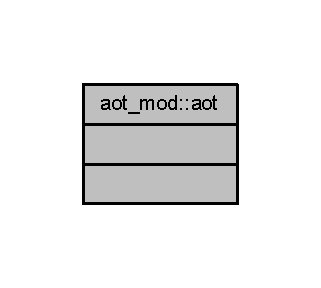
\includegraphics[width=154pt]{interfaceaot__mod_1_1aot__coll__graph}
\end{center}
\end{figure}


\subsection{Detailed Description}


Definition at line 47 of file Ao\+T.\+f90.



The documentation for this interface was generated from the following file\+:\begin{DoxyCompactItemize}
\item 
C\+:/\+Users/administrator/\+Documents/\+Git\+Hub/\+M\+O\+H\+I\+D-\/\+Lagrangian/src/lib/\mbox{\hyperlink{_ao_t_8f90}{Ao\+T.\+f90}}\end{DoxyCompactItemize}

\hypertarget{structaot__mod_1_1aot__class}{}\section{aot\+\_\+mod\+:\+:aot\+\_\+class Type Reference}
\label{structaot__mod_1_1aot__class}\index{aot\+\_\+mod\+::aot\+\_\+class@{aot\+\_\+mod\+::aot\+\_\+class}}


Arrays of Tracers class.  




Collaboration diagram for aot\+\_\+mod\+:\+:aot\+\_\+class\+:\nopagebreak
\begin{figure}[H]
\begin{center}
\leavevmode
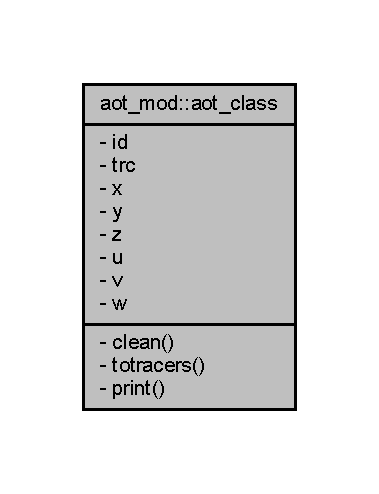
\includegraphics[width=182pt]{structaot__mod_1_1aot__class__coll__graph}
\end{center}
\end{figure}
\subsection*{Private Member Functions}
\begin{DoxyCompactItemize}
\item 
procedure \mbox{\hyperlink{structaot__mod_1_1aot__class_aab1eb00e5cd2868ff08fcd5bb1529688}{clean}}
\item 
procedure \mbox{\hyperlink{structaot__mod_1_1aot__class_a834962484645337446945ae834ea5293}{totracers}}
\item 
procedure \mbox{\hyperlink{structaot__mod_1_1aot__class_a92925f914d4cc5f252e4ca638e104628}{print}} =$>$ print\+\_\+\+AoT
\item 
procedure \mbox{\hyperlink{structaot__mod_1_1aot__class_a9e102da285babd08bff501efbe3b3b10}{detailedprint}} =$>$ Deeprint\+\_\+\+AoT
\end{DoxyCompactItemize}
\subsection*{Private Attributes}
\begin{DoxyCompactItemize}
\item 
integer, dimension(\+:), allocatable \mbox{\hyperlink{structaot__mod_1_1aot__class_ad4bc41c8c0f5dc4ade794eae2d2d5cd5}{id}}
\begin{DoxyCompactList}\small\item\em Id of the Tracer. \end{DoxyCompactList}\item 
class(\mbox{\hyperlink{structaot__mod_1_1trc__ptr__class}{trc\+\_\+ptr\+\_\+class}}), dimension(\+:), allocatable \mbox{\hyperlink{structaot__mod_1_1aot__class_a9f05f9f23b3850d0e79a62d139a633c2}{trc}}
\begin{DoxyCompactList}\small\item\em pointer to the Tracer \end{DoxyCompactList}\item 
real(prec), dimension(\+:), allocatable \mbox{\hyperlink{structaot__mod_1_1aot__class_a4a72558d7ea656f16aca0126e6925725}{x}}
\item 
real(prec), dimension(\+:), allocatable \mbox{\hyperlink{structaot__mod_1_1aot__class_a72bd4c6e0f45ae10286a4a179bda49f0}{y}}
\item 
real(prec), dimension(\+:), allocatable \mbox{\hyperlink{structaot__mod_1_1aot__class_a93f7b7406cbec91c69fdac5bc3505522}{z}}
\begin{DoxyCompactList}\small\item\em coordinates of the Tracer \end{DoxyCompactList}\item 
real(prec), dimension(\+:), allocatable \mbox{\hyperlink{structaot__mod_1_1aot__class_a3aab3baa9fb76719b7d2179d0be7879c}{u}}
\item 
real(prec), dimension(\+:), allocatable \mbox{\hyperlink{structaot__mod_1_1aot__class_a5ff46826ac545ade3a41d66c174870f8}{v}}
\item 
real(prec), dimension(\+:), allocatable \mbox{\hyperlink{structaot__mod_1_1aot__class_a6ec825475ad78b546b7067afec0d043f}{w}}
\begin{DoxyCompactList}\small\item\em velocities of the Tracer \end{DoxyCompactList}\end{DoxyCompactItemize}


\subsection{Detailed Description}
Arrays of Tracers class. 

Definition at line 35 of file Ao\+T.\+f90.



\subsection{Member Function/\+Subroutine Documentation}
\mbox{\Hypertarget{structaot__mod_1_1aot__class_aab1eb00e5cd2868ff08fcd5bb1529688}\label{structaot__mod_1_1aot__class_aab1eb00e5cd2868ff08fcd5bb1529688}} 
\index{aot\+\_\+mod\+::aot\+\_\+class@{aot\+\_\+mod\+::aot\+\_\+class}!clean@{clean}}
\index{clean@{clean}!aot\+\_\+mod\+::aot\+\_\+class@{aot\+\_\+mod\+::aot\+\_\+class}}
\subsubsection{\texorpdfstring{clean()}{clean()}}
{\footnotesize\ttfamily procedure aot\+\_\+mod\+::aot\+\_\+class\+::clean (\begin{DoxyParamCaption}{ }\end{DoxyParamCaption})\hspace{0.3cm}{\ttfamily [private]}}



Definition at line 41 of file Ao\+T.\+f90.

\mbox{\Hypertarget{structaot__mod_1_1aot__class_a9e102da285babd08bff501efbe3b3b10}\label{structaot__mod_1_1aot__class_a9e102da285babd08bff501efbe3b3b10}} 
\index{aot\+\_\+mod\+::aot\+\_\+class@{aot\+\_\+mod\+::aot\+\_\+class}!detailedprint@{detailedprint}}
\index{detailedprint@{detailedprint}!aot\+\_\+mod\+::aot\+\_\+class@{aot\+\_\+mod\+::aot\+\_\+class}}
\subsubsection{\texorpdfstring{detailedprint()}{detailedprint()}}
{\footnotesize\ttfamily procedure aot\+\_\+mod\+::aot\+\_\+class\+::detailedprint (\begin{DoxyParamCaption}{ }\end{DoxyParamCaption})\hspace{0.3cm}{\ttfamily [private]}}



Definition at line 44 of file Ao\+T.\+f90.

\mbox{\Hypertarget{structaot__mod_1_1aot__class_a92925f914d4cc5f252e4ca638e104628}\label{structaot__mod_1_1aot__class_a92925f914d4cc5f252e4ca638e104628}} 
\index{aot\+\_\+mod\+::aot\+\_\+class@{aot\+\_\+mod\+::aot\+\_\+class}!print@{print}}
\index{print@{print}!aot\+\_\+mod\+::aot\+\_\+class@{aot\+\_\+mod\+::aot\+\_\+class}}
\subsubsection{\texorpdfstring{print()}{print()}}
{\footnotesize\ttfamily procedure aot\+\_\+mod\+::aot\+\_\+class\+::print (\begin{DoxyParamCaption}{ }\end{DoxyParamCaption})\hspace{0.3cm}{\ttfamily [private]}}



Definition at line 43 of file Ao\+T.\+f90.

\mbox{\Hypertarget{structaot__mod_1_1aot__class_a834962484645337446945ae834ea5293}\label{structaot__mod_1_1aot__class_a834962484645337446945ae834ea5293}} 
\index{aot\+\_\+mod\+::aot\+\_\+class@{aot\+\_\+mod\+::aot\+\_\+class}!totracers@{totracers}}
\index{totracers@{totracers}!aot\+\_\+mod\+::aot\+\_\+class@{aot\+\_\+mod\+::aot\+\_\+class}}
\subsubsection{\texorpdfstring{totracers()}{totracers()}}
{\footnotesize\ttfamily procedure aot\+\_\+mod\+::aot\+\_\+class\+::totracers (\begin{DoxyParamCaption}{ }\end{DoxyParamCaption})\hspace{0.3cm}{\ttfamily [private]}}



Definition at line 42 of file Ao\+T.\+f90.



\subsection{Member Data Documentation}
\mbox{\Hypertarget{structaot__mod_1_1aot__class_ad4bc41c8c0f5dc4ade794eae2d2d5cd5}\label{structaot__mod_1_1aot__class_ad4bc41c8c0f5dc4ade794eae2d2d5cd5}} 
\index{aot\+\_\+mod\+::aot\+\_\+class@{aot\+\_\+mod\+::aot\+\_\+class}!id@{id}}
\index{id@{id}!aot\+\_\+mod\+::aot\+\_\+class@{aot\+\_\+mod\+::aot\+\_\+class}}
\subsubsection{\texorpdfstring{id}{id}}
{\footnotesize\ttfamily integer, dimension(\+:), allocatable aot\+\_\+mod\+::aot\+\_\+class\+::id\hspace{0.3cm}{\ttfamily [private]}}



Id of the Tracer. 



Definition at line 36 of file Ao\+T.\+f90.


\begin{DoxyCode}
36         \textcolor{keywordtype}{integer}, \textcolor{keywordtype}{allocatable}, \textcolor{keywordtype}{dimension(:)} :: id
\end{DoxyCode}
\mbox{\Hypertarget{structaot__mod_1_1aot__class_a9f05f9f23b3850d0e79a62d139a633c2}\label{structaot__mod_1_1aot__class_a9f05f9f23b3850d0e79a62d139a633c2}} 
\index{aot\+\_\+mod\+::aot\+\_\+class@{aot\+\_\+mod\+::aot\+\_\+class}!trc@{trc}}
\index{trc@{trc}!aot\+\_\+mod\+::aot\+\_\+class@{aot\+\_\+mod\+::aot\+\_\+class}}
\subsubsection{\texorpdfstring{trc}{trc}}
{\footnotesize\ttfamily class(\mbox{\hyperlink{structaot__mod_1_1trc__ptr__class}{trc\+\_\+ptr\+\_\+class}}), dimension(\+:), allocatable aot\+\_\+mod\+::aot\+\_\+class\+::trc\hspace{0.3cm}{\ttfamily [private]}}



pointer to the Tracer 



Definition at line 37 of file Ao\+T.\+f90.


\begin{DoxyCode}
37         \textcolor{keywordtype}{class}(trc\_ptr\_class), \textcolor{keywordtype}{allocatable}, \textcolor{keywordtype}{dimension(:)} :: trc
\end{DoxyCode}
\mbox{\Hypertarget{structaot__mod_1_1aot__class_a3aab3baa9fb76719b7d2179d0be7879c}\label{structaot__mod_1_1aot__class_a3aab3baa9fb76719b7d2179d0be7879c}} 
\index{aot\+\_\+mod\+::aot\+\_\+class@{aot\+\_\+mod\+::aot\+\_\+class}!u@{u}}
\index{u@{u}!aot\+\_\+mod\+::aot\+\_\+class@{aot\+\_\+mod\+::aot\+\_\+class}}
\subsubsection{\texorpdfstring{u}{u}}
{\footnotesize\ttfamily real(prec), dimension(\+:), allocatable aot\+\_\+mod\+::aot\+\_\+class\+::u\hspace{0.3cm}{\ttfamily [private]}}



Definition at line 39 of file Ao\+T.\+f90.


\begin{DoxyCode}
39         \textcolor{keywordtype}{real(prec)}, \textcolor{keywordtype}{allocatable}, \textcolor{keywordtype}{dimension(:)} :: u,v,w
\end{DoxyCode}
\mbox{\Hypertarget{structaot__mod_1_1aot__class_a5ff46826ac545ade3a41d66c174870f8}\label{structaot__mod_1_1aot__class_a5ff46826ac545ade3a41d66c174870f8}} 
\index{aot\+\_\+mod\+::aot\+\_\+class@{aot\+\_\+mod\+::aot\+\_\+class}!v@{v}}
\index{v@{v}!aot\+\_\+mod\+::aot\+\_\+class@{aot\+\_\+mod\+::aot\+\_\+class}}
\subsubsection{\texorpdfstring{v}{v}}
{\footnotesize\ttfamily real(prec), dimension(\+:), allocatable aot\+\_\+mod\+::aot\+\_\+class\+::v\hspace{0.3cm}{\ttfamily [private]}}



Definition at line 39 of file Ao\+T.\+f90.

\mbox{\Hypertarget{structaot__mod_1_1aot__class_a6ec825475ad78b546b7067afec0d043f}\label{structaot__mod_1_1aot__class_a6ec825475ad78b546b7067afec0d043f}} 
\index{aot\+\_\+mod\+::aot\+\_\+class@{aot\+\_\+mod\+::aot\+\_\+class}!w@{w}}
\index{w@{w}!aot\+\_\+mod\+::aot\+\_\+class@{aot\+\_\+mod\+::aot\+\_\+class}}
\subsubsection{\texorpdfstring{w}{w}}
{\footnotesize\ttfamily real(prec), dimension(\+:), allocatable aot\+\_\+mod\+::aot\+\_\+class\+::w\hspace{0.3cm}{\ttfamily [private]}}



velocities of the Tracer 



Definition at line 39 of file Ao\+T.\+f90.

\mbox{\Hypertarget{structaot__mod_1_1aot__class_a4a72558d7ea656f16aca0126e6925725}\label{structaot__mod_1_1aot__class_a4a72558d7ea656f16aca0126e6925725}} 
\index{aot\+\_\+mod\+::aot\+\_\+class@{aot\+\_\+mod\+::aot\+\_\+class}!x@{x}}
\index{x@{x}!aot\+\_\+mod\+::aot\+\_\+class@{aot\+\_\+mod\+::aot\+\_\+class}}
\subsubsection{\texorpdfstring{x}{x}}
{\footnotesize\ttfamily real(prec), dimension(\+:), allocatable aot\+\_\+mod\+::aot\+\_\+class\+::x\hspace{0.3cm}{\ttfamily [private]}}



Definition at line 38 of file Ao\+T.\+f90.


\begin{DoxyCode}
38         \textcolor{keywordtype}{real(prec)}, \textcolor{keywordtype}{allocatable}, \textcolor{keywordtype}{dimension(:)} :: x,y,z
\end{DoxyCode}
\mbox{\Hypertarget{structaot__mod_1_1aot__class_a72bd4c6e0f45ae10286a4a179bda49f0}\label{structaot__mod_1_1aot__class_a72bd4c6e0f45ae10286a4a179bda49f0}} 
\index{aot\+\_\+mod\+::aot\+\_\+class@{aot\+\_\+mod\+::aot\+\_\+class}!y@{y}}
\index{y@{y}!aot\+\_\+mod\+::aot\+\_\+class@{aot\+\_\+mod\+::aot\+\_\+class}}
\subsubsection{\texorpdfstring{y}{y}}
{\footnotesize\ttfamily real(prec), dimension(\+:), allocatable aot\+\_\+mod\+::aot\+\_\+class\+::y\hspace{0.3cm}{\ttfamily [private]}}



Definition at line 38 of file Ao\+T.\+f90.

\mbox{\Hypertarget{structaot__mod_1_1aot__class_a93f7b7406cbec91c69fdac5bc3505522}\label{structaot__mod_1_1aot__class_a93f7b7406cbec91c69fdac5bc3505522}} 
\index{aot\+\_\+mod\+::aot\+\_\+class@{aot\+\_\+mod\+::aot\+\_\+class}!z@{z}}
\index{z@{z}!aot\+\_\+mod\+::aot\+\_\+class@{aot\+\_\+mod\+::aot\+\_\+class}}
\subsubsection{\texorpdfstring{z}{z}}
{\footnotesize\ttfamily real(prec), dimension(\+:), allocatable aot\+\_\+mod\+::aot\+\_\+class\+::z\hspace{0.3cm}{\ttfamily [private]}}



coordinates of the Tracer 



Definition at line 38 of file Ao\+T.\+f90.



The documentation for this type was generated from the following file\+:\begin{DoxyCompactItemize}
\item 
C\+:/\+Users/\+R\+B\+C\+\_\+workhorse/\+Documents/\+Git\+Hub/\+M\+O\+H\+I\+D-\/\+Lagrangian/src/\+M\+O\+H\+I\+D\+Lagrangian\+Lib/\mbox{\hyperlink{_ao_t_8f90}{Ao\+T.\+f90}}\end{DoxyCompactItemize}

\hypertarget{interfacebackground__mod_1_1background}{}\section{background\+\_\+mod\+:\+:background Interface Reference}
\label{interfacebackground__mod_1_1background}\index{background\+\_\+mod\+::background@{background\+\_\+mod\+::background}}


Collaboration diagram for background\+\_\+mod\+:\+:background\+:\nopagebreak
\begin{figure}[H]
\begin{center}
\leavevmode
\includegraphics[width=227pt]{interfacebackground__mod_1_1background__coll__graph}
\end{center}
\end{figure}


\subsection{Detailed Description}


Definition at line 69 of file background.\+f90.



The documentation for this interface was generated from the following file\+:\begin{DoxyCompactItemize}
\item 
C\+:/\+Users/\+R\+B\+C\+\_\+workhorse/\+Documents/\+Git\+Hub/\+M\+O\+H\+I\+D-\/\+Lagrangian/src/\+M\+O\+H\+I\+D\+Lagrangian\+Lib/\mbox{\hyperlink{background_8f90}{background.\+f90}}\end{DoxyCompactItemize}

\hypertarget{structbackground__mod_1_1background__class}{}\section{background\+\_\+mod\+:\+:background\+\_\+class Type Reference}
\label{structbackground__mod_1_1background__class}\index{background\+\_\+mod\+::background\+\_\+class@{background\+\_\+mod\+::background\+\_\+class}}


Collaboration diagram for background\+\_\+mod\+:\+:background\+\_\+class\+:
\nopagebreak
\begin{figure}[H]
\begin{center}
\leavevmode
\includegraphics[width=339pt]{structbackground__mod_1_1background__class__coll__graph}
\end{center}
\end{figure}
\subsection*{Private Member Functions}
\begin{DoxyCompactItemize}
\item 
procedure \mbox{\hyperlink{structbackground__mod_1_1background__class_adbf91df5efe766dead76d836cb0663c4}{add}} =$>$ add\+Field
\item 
procedure \mbox{\hyperlink{structbackground__mod_1_1background__class_a91992b0ccc0956daecda2f250ba934d6}{getdimindex}}
\item 
procedure \mbox{\hyperlink{structbackground__mod_1_1background__class_adecdce1f527c3ccb5f57d8b267023f4f}{getdimextents}}
\item 
procedure \mbox{\hyperlink{structbackground__mod_1_1background__class_a2d01f214966eea8a261c03a39d36743a}{append}} =$>$ append\+Background\+By\+Time
\item 
procedure \mbox{\hyperlink{structbackground__mod_1_1background__class_acb4a97a67f51e509fade50ed4b085f07}{gethyperslab}}
\item 
procedure \mbox{\hyperlink{structbackground__mod_1_1background__class_adbeedbb2d82107fe8dca02b72ffadcec}{shedmemory}}
\item 
procedure \mbox{\hyperlink{structbackground__mod_1_1background__class_a1995f020f28b9800b39a265dfce1f868}{makelandmask}}
\item 
procedure, private \mbox{\hyperlink{structbackground__mod_1_1background__class_ac7e39271ba1838a3f1548f10ff658de1}{getslabdim}}
\item 
procedure, private \mbox{\hyperlink{structbackground__mod_1_1background__class_a12daf122cea65ebd459e8507ae2389fa}{getpointdimindexes}}
\item 
procedure \mbox{\hyperlink{structbackground__mod_1_1background__class_aa41872e2623f1fb7da1fd4b930e6b100}{finalize}} =$>$ clean\+Background
\item 
procedure, private \mbox{\hyperlink{structbackground__mod_1_1background__class_ae4dfe47f7233a9755631095933ed6276}{cleanfields}}
\item 
procedure, private \mbox{\hyperlink{structbackground__mod_1_1background__class_a5a4418427175db3e0d549fc328369993}{setdims}}
\item 
procedure, private \mbox{\hyperlink{structbackground__mod_1_1background__class_a2265e90a0a0685465a17721576919af5}{setextents}}
\item 
procedure, private \mbox{\hyperlink{structbackground__mod_1_1background__class_aa9fde21edbd805c17a6610d9db2ef4a4}{setid}}
\item 
procedure \mbox{\hyperlink{structbackground__mod_1_1background__class_ac6df939097034b1b810ab1e4dca9857a}{check}}
\item 
procedure \mbox{\hyperlink{structbackground__mod_1_1background__class_abe7c9e689ba522cbd15754980ef1cc47}{test}}
\item 
procedure \mbox{\hyperlink{structbackground__mod_1_1background__class_aa1c611fb6813d423cba8f53bdf25465d}{print}} =$>$ print\+Background
\end{DoxyCompactItemize}
\subsection*{Private Attributes}
\begin{DoxyCompactItemize}
\item 
logical \mbox{\hyperlink{structbackground__mod_1_1background__class_aeb3f1a195165888bc63066aed03d651b}{initialized}} = .false.
\item 
integer \mbox{\hyperlink{structbackground__mod_1_1background__class_a1b3eabdda94ffdb97b6bb0db385edfd8}{id}} = 0
\begin{DoxyCompactList}\small\item\em ID of the Background. \end{DoxyCompactList}\item 
type(string) \mbox{\hyperlink{structbackground__mod_1_1background__class_a4f812fd2adfe5d1e50db63e75e460022}{name}}
\begin{DoxyCompactList}\small\item\em Name of the Background. \end{DoxyCompactList}\item 
type(\mbox{\hyperlink{structgeometry__mod_1_1box}{box}}) \mbox{\hyperlink{structbackground__mod_1_1background__class_acaaef54168dbee2731a99d0852844844}{extents}}
\begin{DoxyCompactList}\small\item\em shape\+::box that defines the extents of the Background solution \end{DoxyCompactList}\item 
type(scalar1d\+\_\+field\+\_\+class), dimension(\+:), allocatable \mbox{\hyperlink{structbackground__mod_1_1background__class_a086f319ce4f039190699578d69927013}{dim}}
\begin{DoxyCompactList}\small\item\em Dimensions of the Background fields (time,lon,lat,level for example) \end{DoxyCompactList}\item 
logical, dimension(\+:), allocatable \mbox{\hyperlink{structbackground__mod_1_1background__class_a78b62368ed110d33fd809e8ff101839b}{regulardim}}
\begin{DoxyCompactList}\small\item\em Logical that points. \end{DoxyCompactList}\item 
type(\mbox{\hyperlink{structbackground__mod_1_1fieldslist__class}{fieldslist\+\_\+class}}) \mbox{\hyperlink{structbackground__mod_1_1background__class_a68b750f0476dc75b886638a45a45f8f6}{fields}}
\begin{DoxyCompactList}\small\item\em Linked list to store the fields in the Background. \end{DoxyCompactList}\end{DoxyCompactItemize}


\subsection{Detailed Description}


Definition at line 37 of file background.\+f90.



\subsection{Member Function/\+Subroutine Documentation}
\mbox{\Hypertarget{structbackground__mod_1_1background__class_adbf91df5efe766dead76d836cb0663c4}\label{structbackground__mod_1_1background__class_adbf91df5efe766dead76d836cb0663c4}} 
\index{background\+\_\+mod\+::background\+\_\+class@{background\+\_\+mod\+::background\+\_\+class}!add@{add}}
\index{add@{add}!background\+\_\+mod\+::background\+\_\+class@{background\+\_\+mod\+::background\+\_\+class}}
\subsubsection{\texorpdfstring{add()}{add()}}
{\footnotesize\ttfamily procedure background\+\_\+mod\+::background\+\_\+class\+::add (\begin{DoxyParamCaption}{ }\end{DoxyParamCaption})\hspace{0.3cm}{\ttfamily [private]}}



Definition at line 46 of file background.\+f90.

\mbox{\Hypertarget{structbackground__mod_1_1background__class_a2d01f214966eea8a261c03a39d36743a}\label{structbackground__mod_1_1background__class_a2d01f214966eea8a261c03a39d36743a}} 
\index{background\+\_\+mod\+::background\+\_\+class@{background\+\_\+mod\+::background\+\_\+class}!append@{append}}
\index{append@{append}!background\+\_\+mod\+::background\+\_\+class@{background\+\_\+mod\+::background\+\_\+class}}
\subsubsection{\texorpdfstring{append()}{append()}}
{\footnotesize\ttfamily procedure background\+\_\+mod\+::background\+\_\+class\+::append (\begin{DoxyParamCaption}{ }\end{DoxyParamCaption})\hspace{0.3cm}{\ttfamily [private]}}



Definition at line 49 of file background.\+f90.

\mbox{\Hypertarget{structbackground__mod_1_1background__class_ac6df939097034b1b810ab1e4dca9857a}\label{structbackground__mod_1_1background__class_ac6df939097034b1b810ab1e4dca9857a}} 
\index{background\+\_\+mod\+::background\+\_\+class@{background\+\_\+mod\+::background\+\_\+class}!check@{check}}
\index{check@{check}!background\+\_\+mod\+::background\+\_\+class@{background\+\_\+mod\+::background\+\_\+class}}
\subsubsection{\texorpdfstring{check()}{check()}}
{\footnotesize\ttfamily procedure background\+\_\+mod\+::background\+\_\+class\+::check (\begin{DoxyParamCaption}{ }\end{DoxyParamCaption})\hspace{0.3cm}{\ttfamily [private]}}



Definition at line 60 of file background.\+f90.

\mbox{\Hypertarget{structbackground__mod_1_1background__class_ae4dfe47f7233a9755631095933ed6276}\label{structbackground__mod_1_1background__class_ae4dfe47f7233a9755631095933ed6276}} 
\index{background\+\_\+mod\+::background\+\_\+class@{background\+\_\+mod\+::background\+\_\+class}!cleanfields@{cleanfields}}
\index{cleanfields@{cleanfields}!background\+\_\+mod\+::background\+\_\+class@{background\+\_\+mod\+::background\+\_\+class}}
\subsubsection{\texorpdfstring{cleanfields()}{cleanfields()}}
{\footnotesize\ttfamily procedure, private background\+\_\+mod\+::background\+\_\+class\+::cleanfields (\begin{DoxyParamCaption}{ }\end{DoxyParamCaption})\hspace{0.3cm}{\ttfamily [private]}}



Definition at line 56 of file background.\+f90.

\mbox{\Hypertarget{structbackground__mod_1_1background__class_aa41872e2623f1fb7da1fd4b930e6b100}\label{structbackground__mod_1_1background__class_aa41872e2623f1fb7da1fd4b930e6b100}} 
\index{background\+\_\+mod\+::background\+\_\+class@{background\+\_\+mod\+::background\+\_\+class}!finalize@{finalize}}
\index{finalize@{finalize}!background\+\_\+mod\+::background\+\_\+class@{background\+\_\+mod\+::background\+\_\+class}}
\subsubsection{\texorpdfstring{finalize()}{finalize()}}
{\footnotesize\ttfamily procedure background\+\_\+mod\+::background\+\_\+class\+::finalize (\begin{DoxyParamCaption}{ }\end{DoxyParamCaption})\hspace{0.3cm}{\ttfamily [private]}}



Definition at line 55 of file background.\+f90.

\mbox{\Hypertarget{structbackground__mod_1_1background__class_adecdce1f527c3ccb5f57d8b267023f4f}\label{structbackground__mod_1_1background__class_adecdce1f527c3ccb5f57d8b267023f4f}} 
\index{background\+\_\+mod\+::background\+\_\+class@{background\+\_\+mod\+::background\+\_\+class}!getdimextents@{getdimextents}}
\index{getdimextents@{getdimextents}!background\+\_\+mod\+::background\+\_\+class@{background\+\_\+mod\+::background\+\_\+class}}
\subsubsection{\texorpdfstring{getdimextents()}{getdimextents()}}
{\footnotesize\ttfamily procedure background\+\_\+mod\+::background\+\_\+class\+::getdimextents (\begin{DoxyParamCaption}{ }\end{DoxyParamCaption})\hspace{0.3cm}{\ttfamily [private]}}



Definition at line 48 of file background.\+f90.

\mbox{\Hypertarget{structbackground__mod_1_1background__class_a91992b0ccc0956daecda2f250ba934d6}\label{structbackground__mod_1_1background__class_a91992b0ccc0956daecda2f250ba934d6}} 
\index{background\+\_\+mod\+::background\+\_\+class@{background\+\_\+mod\+::background\+\_\+class}!getdimindex@{getdimindex}}
\index{getdimindex@{getdimindex}!background\+\_\+mod\+::background\+\_\+class@{background\+\_\+mod\+::background\+\_\+class}}
\subsubsection{\texorpdfstring{getdimindex()}{getdimindex()}}
{\footnotesize\ttfamily procedure background\+\_\+mod\+::background\+\_\+class\+::getdimindex (\begin{DoxyParamCaption}{ }\end{DoxyParamCaption})\hspace{0.3cm}{\ttfamily [private]}}



Definition at line 47 of file background.\+f90.

\mbox{\Hypertarget{structbackground__mod_1_1background__class_acb4a97a67f51e509fade50ed4b085f07}\label{structbackground__mod_1_1background__class_acb4a97a67f51e509fade50ed4b085f07}} 
\index{background\+\_\+mod\+::background\+\_\+class@{background\+\_\+mod\+::background\+\_\+class}!gethyperslab@{gethyperslab}}
\index{gethyperslab@{gethyperslab}!background\+\_\+mod\+::background\+\_\+class@{background\+\_\+mod\+::background\+\_\+class}}
\subsubsection{\texorpdfstring{gethyperslab()}{gethyperslab()}}
{\footnotesize\ttfamily procedure background\+\_\+mod\+::background\+\_\+class\+::gethyperslab (\begin{DoxyParamCaption}{ }\end{DoxyParamCaption})\hspace{0.3cm}{\ttfamily [private]}}



Definition at line 50 of file background.\+f90.

\mbox{\Hypertarget{structbackground__mod_1_1background__class_a12daf122cea65ebd459e8507ae2389fa}\label{structbackground__mod_1_1background__class_a12daf122cea65ebd459e8507ae2389fa}} 
\index{background\+\_\+mod\+::background\+\_\+class@{background\+\_\+mod\+::background\+\_\+class}!getpointdimindexes@{getpointdimindexes}}
\index{getpointdimindexes@{getpointdimindexes}!background\+\_\+mod\+::background\+\_\+class@{background\+\_\+mod\+::background\+\_\+class}}
\subsubsection{\texorpdfstring{getpointdimindexes()}{getpointdimindexes()}}
{\footnotesize\ttfamily procedure, private background\+\_\+mod\+::background\+\_\+class\+::getpointdimindexes (\begin{DoxyParamCaption}{ }\end{DoxyParamCaption})\hspace{0.3cm}{\ttfamily [private]}}



Definition at line 54 of file background.\+f90.

\mbox{\Hypertarget{structbackground__mod_1_1background__class_ac7e39271ba1838a3f1548f10ff658de1}\label{structbackground__mod_1_1background__class_ac7e39271ba1838a3f1548f10ff658de1}} 
\index{background\+\_\+mod\+::background\+\_\+class@{background\+\_\+mod\+::background\+\_\+class}!getslabdim@{getslabdim}}
\index{getslabdim@{getslabdim}!background\+\_\+mod\+::background\+\_\+class@{background\+\_\+mod\+::background\+\_\+class}}
\subsubsection{\texorpdfstring{getslabdim()}{getslabdim()}}
{\footnotesize\ttfamily procedure, private background\+\_\+mod\+::background\+\_\+class\+::getslabdim (\begin{DoxyParamCaption}{ }\end{DoxyParamCaption})\hspace{0.3cm}{\ttfamily [private]}}



Definition at line 53 of file background.\+f90.

\mbox{\Hypertarget{structbackground__mod_1_1background__class_a1995f020f28b9800b39a265dfce1f868}\label{structbackground__mod_1_1background__class_a1995f020f28b9800b39a265dfce1f868}} 
\index{background\+\_\+mod\+::background\+\_\+class@{background\+\_\+mod\+::background\+\_\+class}!makelandmask@{makelandmask}}
\index{makelandmask@{makelandmask}!background\+\_\+mod\+::background\+\_\+class@{background\+\_\+mod\+::background\+\_\+class}}
\subsubsection{\texorpdfstring{makelandmask()}{makelandmask()}}
{\footnotesize\ttfamily procedure background\+\_\+mod\+::background\+\_\+class\+::makelandmask (\begin{DoxyParamCaption}{ }\end{DoxyParamCaption})\hspace{0.3cm}{\ttfamily [private]}}



Definition at line 52 of file background.\+f90.

\mbox{\Hypertarget{structbackground__mod_1_1background__class_aa1c611fb6813d423cba8f53bdf25465d}\label{structbackground__mod_1_1background__class_aa1c611fb6813d423cba8f53bdf25465d}} 
\index{background\+\_\+mod\+::background\+\_\+class@{background\+\_\+mod\+::background\+\_\+class}!print@{print}}
\index{print@{print}!background\+\_\+mod\+::background\+\_\+class@{background\+\_\+mod\+::background\+\_\+class}}
\subsubsection{\texorpdfstring{print()}{print()}}
{\footnotesize\ttfamily procedure background\+\_\+mod\+::background\+\_\+class\+::print (\begin{DoxyParamCaption}{ }\end{DoxyParamCaption})\hspace{0.3cm}{\ttfamily [private]}}



Definition at line 62 of file background.\+f90.

\mbox{\Hypertarget{structbackground__mod_1_1background__class_a5a4418427175db3e0d549fc328369993}\label{structbackground__mod_1_1background__class_a5a4418427175db3e0d549fc328369993}} 
\index{background\+\_\+mod\+::background\+\_\+class@{background\+\_\+mod\+::background\+\_\+class}!setdims@{setdims}}
\index{setdims@{setdims}!background\+\_\+mod\+::background\+\_\+class@{background\+\_\+mod\+::background\+\_\+class}}
\subsubsection{\texorpdfstring{setdims()}{setdims()}}
{\footnotesize\ttfamily procedure, private background\+\_\+mod\+::background\+\_\+class\+::setdims (\begin{DoxyParamCaption}{ }\end{DoxyParamCaption})\hspace{0.3cm}{\ttfamily [private]}}



Definition at line 57 of file background.\+f90.

\mbox{\Hypertarget{structbackground__mod_1_1background__class_a2265e90a0a0685465a17721576919af5}\label{structbackground__mod_1_1background__class_a2265e90a0a0685465a17721576919af5}} 
\index{background\+\_\+mod\+::background\+\_\+class@{background\+\_\+mod\+::background\+\_\+class}!setextents@{setextents}}
\index{setextents@{setextents}!background\+\_\+mod\+::background\+\_\+class@{background\+\_\+mod\+::background\+\_\+class}}
\subsubsection{\texorpdfstring{setextents()}{setextents()}}
{\footnotesize\ttfamily procedure, private background\+\_\+mod\+::background\+\_\+class\+::setextents (\begin{DoxyParamCaption}{ }\end{DoxyParamCaption})\hspace{0.3cm}{\ttfamily [private]}}



Definition at line 58 of file background.\+f90.

\mbox{\Hypertarget{structbackground__mod_1_1background__class_aa9fde21edbd805c17a6610d9db2ef4a4}\label{structbackground__mod_1_1background__class_aa9fde21edbd805c17a6610d9db2ef4a4}} 
\index{background\+\_\+mod\+::background\+\_\+class@{background\+\_\+mod\+::background\+\_\+class}!setid@{setid}}
\index{setid@{setid}!background\+\_\+mod\+::background\+\_\+class@{background\+\_\+mod\+::background\+\_\+class}}
\subsubsection{\texorpdfstring{setid()}{setid()}}
{\footnotesize\ttfamily procedure, private background\+\_\+mod\+::background\+\_\+class\+::setid (\begin{DoxyParamCaption}{ }\end{DoxyParamCaption})\hspace{0.3cm}{\ttfamily [private]}}



Definition at line 59 of file background.\+f90.

\mbox{\Hypertarget{structbackground__mod_1_1background__class_adbeedbb2d82107fe8dca02b72ffadcec}\label{structbackground__mod_1_1background__class_adbeedbb2d82107fe8dca02b72ffadcec}} 
\index{background\+\_\+mod\+::background\+\_\+class@{background\+\_\+mod\+::background\+\_\+class}!shedmemory@{shedmemory}}
\index{shedmemory@{shedmemory}!background\+\_\+mod\+::background\+\_\+class@{background\+\_\+mod\+::background\+\_\+class}}
\subsubsection{\texorpdfstring{shedmemory()}{shedmemory()}}
{\footnotesize\ttfamily procedure background\+\_\+mod\+::background\+\_\+class\+::shedmemory (\begin{DoxyParamCaption}{ }\end{DoxyParamCaption})\hspace{0.3cm}{\ttfamily [private]}}



Definition at line 51 of file background.\+f90.

\mbox{\Hypertarget{structbackground__mod_1_1background__class_abe7c9e689ba522cbd15754980ef1cc47}\label{structbackground__mod_1_1background__class_abe7c9e689ba522cbd15754980ef1cc47}} 
\index{background\+\_\+mod\+::background\+\_\+class@{background\+\_\+mod\+::background\+\_\+class}!test@{test}}
\index{test@{test}!background\+\_\+mod\+::background\+\_\+class@{background\+\_\+mod\+::background\+\_\+class}}
\subsubsection{\texorpdfstring{test()}{test()}}
{\footnotesize\ttfamily procedure background\+\_\+mod\+::background\+\_\+class\+::test (\begin{DoxyParamCaption}{ }\end{DoxyParamCaption})\hspace{0.3cm}{\ttfamily [private]}}



Definition at line 61 of file background.\+f90.



\subsection{Member Data Documentation}
\mbox{\Hypertarget{structbackground__mod_1_1background__class_a086f319ce4f039190699578d69927013}\label{structbackground__mod_1_1background__class_a086f319ce4f039190699578d69927013}} 
\index{background\+\_\+mod\+::background\+\_\+class@{background\+\_\+mod\+::background\+\_\+class}!dim@{dim}}
\index{dim@{dim}!background\+\_\+mod\+::background\+\_\+class@{background\+\_\+mod\+::background\+\_\+class}}
\subsubsection{\texorpdfstring{dim}{dim}}
{\footnotesize\ttfamily type(scalar1d\+\_\+field\+\_\+class), dimension(\+:), allocatable background\+\_\+mod\+::background\+\_\+class\+::dim\hspace{0.3cm}{\ttfamily [private]}}



Dimensions of the Background fields (time,lon,lat,level for example) 



Definition at line 42 of file background.\+f90.


\begin{DoxyCode}
42         \textcolor{keywordtype}{type}(scalar1d\_field\_class), \textcolor{keywordtype}{allocatable}, \textcolor{keywordtype}{dimension(:)} :: dim
\end{DoxyCode}
\mbox{\Hypertarget{structbackground__mod_1_1background__class_acaaef54168dbee2731a99d0852844844}\label{structbackground__mod_1_1background__class_acaaef54168dbee2731a99d0852844844}} 
\index{background\+\_\+mod\+::background\+\_\+class@{background\+\_\+mod\+::background\+\_\+class}!extents@{extents}}
\index{extents@{extents}!background\+\_\+mod\+::background\+\_\+class@{background\+\_\+mod\+::background\+\_\+class}}
\subsubsection{\texorpdfstring{extents}{extents}}
{\footnotesize\ttfamily type(\mbox{\hyperlink{structgeometry__mod_1_1box}{box}}) background\+\_\+mod\+::background\+\_\+class\+::extents\hspace{0.3cm}{\ttfamily [private]}}



shape\+::box that defines the extents of the Background solution 



Definition at line 41 of file background.\+f90.


\begin{DoxyCode}
41         \textcolor{keywordtype}{type}(box) :: extents
\end{DoxyCode}
\mbox{\Hypertarget{structbackground__mod_1_1background__class_a68b750f0476dc75b886638a45a45f8f6}\label{structbackground__mod_1_1background__class_a68b750f0476dc75b886638a45a45f8f6}} 
\index{background\+\_\+mod\+::background\+\_\+class@{background\+\_\+mod\+::background\+\_\+class}!fields@{fields}}
\index{fields@{fields}!background\+\_\+mod\+::background\+\_\+class@{background\+\_\+mod\+::background\+\_\+class}}
\subsubsection{\texorpdfstring{fields}{fields}}
{\footnotesize\ttfamily type(\mbox{\hyperlink{structbackground__mod_1_1fieldslist__class}{fieldslist\+\_\+class}}) background\+\_\+mod\+::background\+\_\+class\+::fields\hspace{0.3cm}{\ttfamily [private]}}



Linked list to store the fields in the Background. 



Definition at line 44 of file background.\+f90.


\begin{DoxyCode}
44         \textcolor{keywordtype}{type}(fieldsList\_class) :: fields
\end{DoxyCode}
\mbox{\Hypertarget{structbackground__mod_1_1background__class_a1b3eabdda94ffdb97b6bb0db385edfd8}\label{structbackground__mod_1_1background__class_a1b3eabdda94ffdb97b6bb0db385edfd8}} 
\index{background\+\_\+mod\+::background\+\_\+class@{background\+\_\+mod\+::background\+\_\+class}!id@{id}}
\index{id@{id}!background\+\_\+mod\+::background\+\_\+class@{background\+\_\+mod\+::background\+\_\+class}}
\subsubsection{\texorpdfstring{id}{id}}
{\footnotesize\ttfamily integer background\+\_\+mod\+::background\+\_\+class\+::id = 0\hspace{0.3cm}{\ttfamily [private]}}



ID of the Background. 



Definition at line 39 of file background.\+f90.


\begin{DoxyCode}
39         \textcolor{keywordtype}{integer} :: id = 0
\end{DoxyCode}
\mbox{\Hypertarget{structbackground__mod_1_1background__class_aeb3f1a195165888bc63066aed03d651b}\label{structbackground__mod_1_1background__class_aeb3f1a195165888bc63066aed03d651b}} 
\index{background\+\_\+mod\+::background\+\_\+class@{background\+\_\+mod\+::background\+\_\+class}!initialized@{initialized}}
\index{initialized@{initialized}!background\+\_\+mod\+::background\+\_\+class@{background\+\_\+mod\+::background\+\_\+class}}
\subsubsection{\texorpdfstring{initialized}{initialized}}
{\footnotesize\ttfamily logical background\+\_\+mod\+::background\+\_\+class\+::initialized = .false.\hspace{0.3cm}{\ttfamily [private]}}



Definition at line 38 of file background.\+f90.


\begin{DoxyCode}
38         \textcolor{keywordtype}{logical} :: initialized = .false.
\end{DoxyCode}
\mbox{\Hypertarget{structbackground__mod_1_1background__class_a4f812fd2adfe5d1e50db63e75e460022}\label{structbackground__mod_1_1background__class_a4f812fd2adfe5d1e50db63e75e460022}} 
\index{background\+\_\+mod\+::background\+\_\+class@{background\+\_\+mod\+::background\+\_\+class}!name@{name}}
\index{name@{name}!background\+\_\+mod\+::background\+\_\+class@{background\+\_\+mod\+::background\+\_\+class}}
\subsubsection{\texorpdfstring{name}{name}}
{\footnotesize\ttfamily type(string) background\+\_\+mod\+::background\+\_\+class\+::name\hspace{0.3cm}{\ttfamily [private]}}



Name of the Background. 



Definition at line 40 of file background.\+f90.


\begin{DoxyCode}
40         \textcolor{keywordtype}{type}(string) :: name
\end{DoxyCode}
\mbox{\Hypertarget{structbackground__mod_1_1background__class_a78b62368ed110d33fd809e8ff101839b}\label{structbackground__mod_1_1background__class_a78b62368ed110d33fd809e8ff101839b}} 
\index{background\+\_\+mod\+::background\+\_\+class@{background\+\_\+mod\+::background\+\_\+class}!regulardim@{regulardim}}
\index{regulardim@{regulardim}!background\+\_\+mod\+::background\+\_\+class@{background\+\_\+mod\+::background\+\_\+class}}
\subsubsection{\texorpdfstring{regulardim}{regulardim}}
{\footnotesize\ttfamily logical, dimension(\+:), allocatable background\+\_\+mod\+::background\+\_\+class\+::regulardim\hspace{0.3cm}{\ttfamily [private]}}



Logical that points. 



Definition at line 43 of file background.\+f90.


\begin{DoxyCode}
43         \textcolor{keywordtype}{logical}, \textcolor{keywordtype}{allocatable}, \textcolor{keywordtype}{dimension(:)} :: regularDim
\end{DoxyCode}


The documentation for this type was generated from the following file\+:\begin{DoxyCompactItemize}
\item 
C\+:/\+Users/\+R\+B\+C\+\_\+workhorse/\+Documents/\+Git\+Hub/\+M\+O\+H\+I\+D-\/\+Lagrangian/src/\+M\+O\+H\+I\+D\+Lagrangian\+Lib/\mbox{\hyperlink{background_8f90}{background.\+f90}}\end{DoxyCompactItemize}

\hypertarget{structblocks__mod_1_1block__class}{}\section{blocks\+\_\+mod\+:\+:block\+\_\+class Type Reference}
\label{structblocks__mod_1_1block__class}\index{blocks\+\_\+mod\+::block\+\_\+class@{blocks\+\_\+mod\+::block\+\_\+class}}


Collaboration diagram for blocks\+\_\+mod\+:\+:block\+\_\+class\+:\nopagebreak
\begin{figure}[H]
\begin{center}
\leavevmode
\includegraphics[width=350pt]{structblocks__mod_1_1block__class__coll__graph}
\end{center}
\end{figure}
\subsection*{Public Member Functions}
\begin{DoxyCompactItemize}
\item 
procedure, public \mbox{\hyperlink{structblocks__mod_1_1block__class_ad671745ca5dc3227ddb0ed1d9ff45268}{initialize}} =$>$ init\+Block
\item 
procedure, public \mbox{\hyperlink{structblocks__mod_1_1block__class_ac79980e841902691a06212dce50f6331}{putsource}}
\item 
procedure, public \mbox{\hyperlink{structblocks__mod_1_1block__class_ad1d0f1aca1323fad86177deb0b818a51}{callemitter}}
\item 
procedure, public \mbox{\hyperlink{structblocks__mod_1_1block__class_a00f8c114e84499356db3f8b633a6b3a3}{distributetracers}}
\item 
procedure, public \mbox{\hyperlink{structblocks__mod_1_1block__class_a73bd9f99f97d7fd882a3ade1103d27ae}{toogleblocksources}}
\item 
procedure, public \mbox{\hyperlink{structblocks__mod_1_1block__class_a68f5bb0cb32b5b51cffd66d472cc45f0}{consolidatearrays}}
\item 
procedure, public \mbox{\hyperlink{structblocks__mod_1_1block__class_ad3521ef8424f47673a2acd15b5bd0545}{tracerstoaot}}
\item 
procedure, public \mbox{\hyperlink{structblocks__mod_1_1block__class_abe738c65f3fecf013c3884275a3fe7e4}{runsolver}}
\item 
procedure, public \mbox{\hyperlink{structblocks__mod_1_1block__class_af7ee4536d72f1a114d9289c9e484f703}{aottotracers}}
\item 
procedure, public \mbox{\hyperlink{structblocks__mod_1_1block__class_ab58da434b2813d158b3f688d3c60d02c}{cleanaot}}
\item 
procedure, public \mbox{\hyperlink{structblocks__mod_1_1block__class_a7a3f2eb6823a683a6aaa2159b50ee990}{numalloctracers}}
\item 
procedure, public \mbox{\hyperlink{structblocks__mod_1_1block__class_a43b4c133934eaadb55d30cf834d1e28c}{print}} =$>$ print\+Block
\item 
procedure, public \mbox{\hyperlink{structblocks__mod_1_1block__class_a937d8dca8393460bc718dafa8a5c03ac}{detailedprint}} =$>$ printdetail\+Block
\end{DoxyCompactItemize}
\subsection*{Private Attributes}
\begin{DoxyCompactItemize}
\item 
integer \mbox{\hyperlink{structblocks__mod_1_1block__class_addd1a493d56aa1ffd1bc27c56b682065}{id}}
\item 
type(\mbox{\hyperlink{structgeometry__mod_1_1box}{box}}) \mbox{\hyperlink{structblocks__mod_1_1block__class_aff3b0cb7d8248f8a87691a028de916d3}{extents}}
\begin{DoxyCompactList}\small\item\em shape\+::box that defines the extents of this block \end{DoxyCompactList}\item 
type(sourcelist\+\_\+class) \mbox{\hyperlink{structblocks__mod_1_1block__class_a2f4d63afb2696e2728f20a99e26a4b18}{lsource}}
\begin{DoxyCompactList}\small\item\em List of Sources currently on this block. \end{DoxyCompactList}\item 
type(\mbox{\hyperlink{structemitter__mod_1_1emitter__class}{emitter\+\_\+class}}) \mbox{\hyperlink{structblocks__mod_1_1block__class_a55e85183ba871abcaba1c00d5393611f}{emitter}}
\begin{DoxyCompactList}\small\item\em Block Emitter. \end{DoxyCompactList}\item 
type(tracerlist\+\_\+class) \mbox{\hyperlink{structblocks__mod_1_1block__class_ab4e2108886a09ba919d01474503f6165}{ltracer}}
\begin{DoxyCompactList}\small\item\em List of Tracers currently on this block. \end{DoxyCompactList}\item 
type(aot\+\_\+class) \mbox{\hyperlink{structblocks__mod_1_1block__class_a53f912fe57eb5e386ca62b1dbd087417}{aot}}
\begin{DoxyCompactList}\small\item\em Block Array of Tracers for actual numerical work. \end{DoxyCompactList}\item 
type(\mbox{\hyperlink{structsolver__mod_1_1solver__class}{solver\+\_\+class}}) \mbox{\hyperlink{structblocks__mod_1_1block__class_a081258113128b3bcdefdbeac4bc5d039}{solver}}
\begin{DoxyCompactList}\small\item\em Block Solver. \end{DoxyCompactList}\item 
type(\mbox{\hyperlink{structbackground__mod_1_1background__class}{background\+\_\+class}}), dimension(\+:), allocatable \mbox{\hyperlink{structblocks__mod_1_1block__class_a774c07bf82d1392236abc81c285ea943}{background}}
\begin{DoxyCompactList}\small\item\em Solution Backgrounds for the Block. \end{DoxyCompactList}\end{DoxyCompactItemize}


\subsection{Detailed Description}


Definition at line 42 of file blocks.\+f90.



\subsection{Member Function/\+Subroutine Documentation}
\mbox{\Hypertarget{structblocks__mod_1_1block__class_af7ee4536d72f1a114d9289c9e484f703}\label{structblocks__mod_1_1block__class_af7ee4536d72f1a114d9289c9e484f703}} 
\index{blocks\+\_\+mod\+::block\+\_\+class@{blocks\+\_\+mod\+::block\+\_\+class}!aottotracers@{aottotracers}}
\index{aottotracers@{aottotracers}!blocks\+\_\+mod\+::block\+\_\+class@{blocks\+\_\+mod\+::block\+\_\+class}}
\subsubsection{\texorpdfstring{aottotracers()}{aottotracers()}}
{\footnotesize\ttfamily procedure, public blocks\+\_\+mod\+::block\+\_\+class\+::aottotracers (\begin{DoxyParamCaption}{ }\end{DoxyParamCaption})}



Definition at line 61 of file blocks.\+f90.

\mbox{\Hypertarget{structblocks__mod_1_1block__class_ad1d0f1aca1323fad86177deb0b818a51}\label{structblocks__mod_1_1block__class_ad1d0f1aca1323fad86177deb0b818a51}} 
\index{blocks\+\_\+mod\+::block\+\_\+class@{blocks\+\_\+mod\+::block\+\_\+class}!callemitter@{callemitter}}
\index{callemitter@{callemitter}!blocks\+\_\+mod\+::block\+\_\+class@{blocks\+\_\+mod\+::block\+\_\+class}}
\subsubsection{\texorpdfstring{callemitter()}{callemitter()}}
{\footnotesize\ttfamily procedure, public blocks\+\_\+mod\+::block\+\_\+class\+::callemitter (\begin{DoxyParamCaption}{ }\end{DoxyParamCaption})}



Definition at line 55 of file blocks.\+f90.

\mbox{\Hypertarget{structblocks__mod_1_1block__class_ab58da434b2813d158b3f688d3c60d02c}\label{structblocks__mod_1_1block__class_ab58da434b2813d158b3f688d3c60d02c}} 
\index{blocks\+\_\+mod\+::block\+\_\+class@{blocks\+\_\+mod\+::block\+\_\+class}!cleanaot@{cleanaot}}
\index{cleanaot@{cleanaot}!blocks\+\_\+mod\+::block\+\_\+class@{blocks\+\_\+mod\+::block\+\_\+class}}
\subsubsection{\texorpdfstring{cleanaot()}{cleanaot()}}
{\footnotesize\ttfamily procedure, public blocks\+\_\+mod\+::block\+\_\+class\+::cleanaot (\begin{DoxyParamCaption}{ }\end{DoxyParamCaption})}



Definition at line 62 of file blocks.\+f90.

\mbox{\Hypertarget{structblocks__mod_1_1block__class_a68f5bb0cb32b5b51cffd66d472cc45f0}\label{structblocks__mod_1_1block__class_a68f5bb0cb32b5b51cffd66d472cc45f0}} 
\index{blocks\+\_\+mod\+::block\+\_\+class@{blocks\+\_\+mod\+::block\+\_\+class}!consolidatearrays@{consolidatearrays}}
\index{consolidatearrays@{consolidatearrays}!blocks\+\_\+mod\+::block\+\_\+class@{blocks\+\_\+mod\+::block\+\_\+class}}
\subsubsection{\texorpdfstring{consolidatearrays()}{consolidatearrays()}}
{\footnotesize\ttfamily procedure, public blocks\+\_\+mod\+::block\+\_\+class\+::consolidatearrays (\begin{DoxyParamCaption}{ }\end{DoxyParamCaption})}



Definition at line 58 of file blocks.\+f90.

\mbox{\Hypertarget{structblocks__mod_1_1block__class_a937d8dca8393460bc718dafa8a5c03ac}\label{structblocks__mod_1_1block__class_a937d8dca8393460bc718dafa8a5c03ac}} 
\index{blocks\+\_\+mod\+::block\+\_\+class@{blocks\+\_\+mod\+::block\+\_\+class}!detailedprint@{detailedprint}}
\index{detailedprint@{detailedprint}!blocks\+\_\+mod\+::block\+\_\+class@{blocks\+\_\+mod\+::block\+\_\+class}}
\subsubsection{\texorpdfstring{detailedprint()}{detailedprint()}}
{\footnotesize\ttfamily procedure, public blocks\+\_\+mod\+::block\+\_\+class\+::detailedprint (\begin{DoxyParamCaption}{ }\end{DoxyParamCaption})}



Definition at line 65 of file blocks.\+f90.

\mbox{\Hypertarget{structblocks__mod_1_1block__class_a00f8c114e84499356db3f8b633a6b3a3}\label{structblocks__mod_1_1block__class_a00f8c114e84499356db3f8b633a6b3a3}} 
\index{blocks\+\_\+mod\+::block\+\_\+class@{blocks\+\_\+mod\+::block\+\_\+class}!distributetracers@{distributetracers}}
\index{distributetracers@{distributetracers}!blocks\+\_\+mod\+::block\+\_\+class@{blocks\+\_\+mod\+::block\+\_\+class}}
\subsubsection{\texorpdfstring{distributetracers()}{distributetracers()}}
{\footnotesize\ttfamily procedure, public blocks\+\_\+mod\+::block\+\_\+class\+::distributetracers (\begin{DoxyParamCaption}{ }\end{DoxyParamCaption})}



Definition at line 56 of file blocks.\+f90.

\mbox{\Hypertarget{structblocks__mod_1_1block__class_ad671745ca5dc3227ddb0ed1d9ff45268}\label{structblocks__mod_1_1block__class_ad671745ca5dc3227ddb0ed1d9ff45268}} 
\index{blocks\+\_\+mod\+::block\+\_\+class@{blocks\+\_\+mod\+::block\+\_\+class}!initialize@{initialize}}
\index{initialize@{initialize}!blocks\+\_\+mod\+::block\+\_\+class@{blocks\+\_\+mod\+::block\+\_\+class}}
\subsubsection{\texorpdfstring{initialize()}{initialize()}}
{\footnotesize\ttfamily procedure, public blocks\+\_\+mod\+::block\+\_\+class\+::initialize (\begin{DoxyParamCaption}{ }\end{DoxyParamCaption})}



Definition at line 53 of file blocks.\+f90.

\mbox{\Hypertarget{structblocks__mod_1_1block__class_a7a3f2eb6823a683a6aaa2159b50ee990}\label{structblocks__mod_1_1block__class_a7a3f2eb6823a683a6aaa2159b50ee990}} 
\index{blocks\+\_\+mod\+::block\+\_\+class@{blocks\+\_\+mod\+::block\+\_\+class}!numalloctracers@{numalloctracers}}
\index{numalloctracers@{numalloctracers}!blocks\+\_\+mod\+::block\+\_\+class@{blocks\+\_\+mod\+::block\+\_\+class}}
\subsubsection{\texorpdfstring{numalloctracers()}{numalloctracers()}}
{\footnotesize\ttfamily procedure, public blocks\+\_\+mod\+::block\+\_\+class\+::numalloctracers (\begin{DoxyParamCaption}{ }\end{DoxyParamCaption})}



Definition at line 63 of file blocks.\+f90.

\mbox{\Hypertarget{structblocks__mod_1_1block__class_a43b4c133934eaadb55d30cf834d1e28c}\label{structblocks__mod_1_1block__class_a43b4c133934eaadb55d30cf834d1e28c}} 
\index{blocks\+\_\+mod\+::block\+\_\+class@{blocks\+\_\+mod\+::block\+\_\+class}!print@{print}}
\index{print@{print}!blocks\+\_\+mod\+::block\+\_\+class@{blocks\+\_\+mod\+::block\+\_\+class}}
\subsubsection{\texorpdfstring{print()}{print()}}
{\footnotesize\ttfamily procedure, public blocks\+\_\+mod\+::block\+\_\+class\+::print (\begin{DoxyParamCaption}{ }\end{DoxyParamCaption})}



Definition at line 64 of file blocks.\+f90.

\mbox{\Hypertarget{structblocks__mod_1_1block__class_ac79980e841902691a06212dce50f6331}\label{structblocks__mod_1_1block__class_ac79980e841902691a06212dce50f6331}} 
\index{blocks\+\_\+mod\+::block\+\_\+class@{blocks\+\_\+mod\+::block\+\_\+class}!putsource@{putsource}}
\index{putsource@{putsource}!blocks\+\_\+mod\+::block\+\_\+class@{blocks\+\_\+mod\+::block\+\_\+class}}
\subsubsection{\texorpdfstring{putsource()}{putsource()}}
{\footnotesize\ttfamily procedure, public blocks\+\_\+mod\+::block\+\_\+class\+::putsource (\begin{DoxyParamCaption}{ }\end{DoxyParamCaption})}



Definition at line 54 of file blocks.\+f90.

\mbox{\Hypertarget{structblocks__mod_1_1block__class_abe738c65f3fecf013c3884275a3fe7e4}\label{structblocks__mod_1_1block__class_abe738c65f3fecf013c3884275a3fe7e4}} 
\index{blocks\+\_\+mod\+::block\+\_\+class@{blocks\+\_\+mod\+::block\+\_\+class}!runsolver@{runsolver}}
\index{runsolver@{runsolver}!blocks\+\_\+mod\+::block\+\_\+class@{blocks\+\_\+mod\+::block\+\_\+class}}
\subsubsection{\texorpdfstring{runsolver()}{runsolver()}}
{\footnotesize\ttfamily procedure, public blocks\+\_\+mod\+::block\+\_\+class\+::runsolver (\begin{DoxyParamCaption}{ }\end{DoxyParamCaption})}



Definition at line 60 of file blocks.\+f90.

\mbox{\Hypertarget{structblocks__mod_1_1block__class_a73bd9f99f97d7fd882a3ade1103d27ae}\label{structblocks__mod_1_1block__class_a73bd9f99f97d7fd882a3ade1103d27ae}} 
\index{blocks\+\_\+mod\+::block\+\_\+class@{blocks\+\_\+mod\+::block\+\_\+class}!toogleblocksources@{toogleblocksources}}
\index{toogleblocksources@{toogleblocksources}!blocks\+\_\+mod\+::block\+\_\+class@{blocks\+\_\+mod\+::block\+\_\+class}}
\subsubsection{\texorpdfstring{toogleblocksources()}{toogleblocksources()}}
{\footnotesize\ttfamily procedure, public blocks\+\_\+mod\+::block\+\_\+class\+::toogleblocksources (\begin{DoxyParamCaption}{ }\end{DoxyParamCaption})}



Definition at line 57 of file blocks.\+f90.

\mbox{\Hypertarget{structblocks__mod_1_1block__class_ad3521ef8424f47673a2acd15b5bd0545}\label{structblocks__mod_1_1block__class_ad3521ef8424f47673a2acd15b5bd0545}} 
\index{blocks\+\_\+mod\+::block\+\_\+class@{blocks\+\_\+mod\+::block\+\_\+class}!tracerstoaot@{tracerstoaot}}
\index{tracerstoaot@{tracerstoaot}!blocks\+\_\+mod\+::block\+\_\+class@{blocks\+\_\+mod\+::block\+\_\+class}}
\subsubsection{\texorpdfstring{tracerstoaot()}{tracerstoaot()}}
{\footnotesize\ttfamily procedure, public blocks\+\_\+mod\+::block\+\_\+class\+::tracerstoaot (\begin{DoxyParamCaption}{ }\end{DoxyParamCaption})}



Definition at line 59 of file blocks.\+f90.



\subsection{Member Data Documentation}
\mbox{\Hypertarget{structblocks__mod_1_1block__class_a53f912fe57eb5e386ca62b1dbd087417}\label{structblocks__mod_1_1block__class_a53f912fe57eb5e386ca62b1dbd087417}} 
\index{blocks\+\_\+mod\+::block\+\_\+class@{blocks\+\_\+mod\+::block\+\_\+class}!aot@{aot}}
\index{aot@{aot}!blocks\+\_\+mod\+::block\+\_\+class@{blocks\+\_\+mod\+::block\+\_\+class}}
\subsubsection{\texorpdfstring{aot}{aot}}
{\footnotesize\ttfamily type(aot\+\_\+class) blocks\+\_\+mod\+::block\+\_\+class\+::aot\hspace{0.3cm}{\ttfamily [private]}}



Block Array of Tracers for actual numerical work. 



Definition at line 48 of file blocks.\+f90.


\begin{DoxyCode}
48         \textcolor{keywordtype}{type}(aot\_class)        :: AoT
\end{DoxyCode}
\mbox{\Hypertarget{structblocks__mod_1_1block__class_a774c07bf82d1392236abc81c285ea943}\label{structblocks__mod_1_1block__class_a774c07bf82d1392236abc81c285ea943}} 
\index{blocks\+\_\+mod\+::block\+\_\+class@{blocks\+\_\+mod\+::block\+\_\+class}!background@{background}}
\index{background@{background}!blocks\+\_\+mod\+::block\+\_\+class@{blocks\+\_\+mod\+::block\+\_\+class}}
\subsubsection{\texorpdfstring{background}{background}}
{\footnotesize\ttfamily type(\mbox{\hyperlink{structbackground__mod_1_1background__class}{background\+\_\+class}}), dimension(\+:), allocatable blocks\+\_\+mod\+::block\+\_\+class\+::background\hspace{0.3cm}{\ttfamily [private]}}



Solution Backgrounds for the Block. 



Definition at line 50 of file blocks.\+f90.


\begin{DoxyCode}
50         \textcolor{keywordtype}{type}(background\_class), \textcolor{keywordtype}{allocatable}, \textcolor{keywordtype}{dimension(:)} :: Background
\end{DoxyCode}
\mbox{\Hypertarget{structblocks__mod_1_1block__class_a55e85183ba871abcaba1c00d5393611f}\label{structblocks__mod_1_1block__class_a55e85183ba871abcaba1c00d5393611f}} 
\index{blocks\+\_\+mod\+::block\+\_\+class@{blocks\+\_\+mod\+::block\+\_\+class}!emitter@{emitter}}
\index{emitter@{emitter}!blocks\+\_\+mod\+::block\+\_\+class@{blocks\+\_\+mod\+::block\+\_\+class}}
\subsubsection{\texorpdfstring{emitter}{emitter}}
{\footnotesize\ttfamily type(\mbox{\hyperlink{structemitter__mod_1_1emitter__class}{emitter\+\_\+class}}) blocks\+\_\+mod\+::block\+\_\+class\+::emitter\hspace{0.3cm}{\ttfamily [private]}}



Block Emitter. 



Definition at line 46 of file blocks.\+f90.


\begin{DoxyCode}
46         \textcolor{keywordtype}{type}(emitter\_class)    :: Emitter
\end{DoxyCode}
\mbox{\Hypertarget{structblocks__mod_1_1block__class_aff3b0cb7d8248f8a87691a028de916d3}\label{structblocks__mod_1_1block__class_aff3b0cb7d8248f8a87691a028de916d3}} 
\index{blocks\+\_\+mod\+::block\+\_\+class@{blocks\+\_\+mod\+::block\+\_\+class}!extents@{extents}}
\index{extents@{extents}!blocks\+\_\+mod\+::block\+\_\+class@{blocks\+\_\+mod\+::block\+\_\+class}}
\subsubsection{\texorpdfstring{extents}{extents}}
{\footnotesize\ttfamily type(\mbox{\hyperlink{structgeometry__mod_1_1box}{box}}) blocks\+\_\+mod\+::block\+\_\+class\+::extents\hspace{0.3cm}{\ttfamily [private]}}



shape\+::box that defines the extents of this block 



Definition at line 44 of file blocks.\+f90.


\begin{DoxyCode}
44         \textcolor{keywordtype}{type}(box) :: extents
\end{DoxyCode}
\mbox{\Hypertarget{structblocks__mod_1_1block__class_addd1a493d56aa1ffd1bc27c56b682065}\label{structblocks__mod_1_1block__class_addd1a493d56aa1ffd1bc27c56b682065}} 
\index{blocks\+\_\+mod\+::block\+\_\+class@{blocks\+\_\+mod\+::block\+\_\+class}!id@{id}}
\index{id@{id}!blocks\+\_\+mod\+::block\+\_\+class@{blocks\+\_\+mod\+::block\+\_\+class}}
\subsubsection{\texorpdfstring{id}{id}}
{\footnotesize\ttfamily integer blocks\+\_\+mod\+::block\+\_\+class\+::id\hspace{0.3cm}{\ttfamily [private]}}



Definition at line 43 of file blocks.\+f90.


\begin{DoxyCode}
43         \textcolor{keywordtype}{integer} :: id
\end{DoxyCode}
\mbox{\Hypertarget{structblocks__mod_1_1block__class_a2f4d63afb2696e2728f20a99e26a4b18}\label{structblocks__mod_1_1block__class_a2f4d63afb2696e2728f20a99e26a4b18}} 
\index{blocks\+\_\+mod\+::block\+\_\+class@{blocks\+\_\+mod\+::block\+\_\+class}!lsource@{lsource}}
\index{lsource@{lsource}!blocks\+\_\+mod\+::block\+\_\+class@{blocks\+\_\+mod\+::block\+\_\+class}}
\subsubsection{\texorpdfstring{lsource}{lsource}}
{\footnotesize\ttfamily type(sourcelist\+\_\+class) blocks\+\_\+mod\+::block\+\_\+class\+::lsource\hspace{0.3cm}{\ttfamily [private]}}



List of Sources currently on this block. 



Definition at line 45 of file blocks.\+f90.


\begin{DoxyCode}
45         \textcolor{keywordtype}{type}(sourceList\_class) :: LSource
\end{DoxyCode}
\mbox{\Hypertarget{structblocks__mod_1_1block__class_ab4e2108886a09ba919d01474503f6165}\label{structblocks__mod_1_1block__class_ab4e2108886a09ba919d01474503f6165}} 
\index{blocks\+\_\+mod\+::block\+\_\+class@{blocks\+\_\+mod\+::block\+\_\+class}!ltracer@{ltracer}}
\index{ltracer@{ltracer}!blocks\+\_\+mod\+::block\+\_\+class@{blocks\+\_\+mod\+::block\+\_\+class}}
\subsubsection{\texorpdfstring{ltracer}{ltracer}}
{\footnotesize\ttfamily type(tracerlist\+\_\+class) blocks\+\_\+mod\+::block\+\_\+class\+::ltracer\hspace{0.3cm}{\ttfamily [private]}}



List of Tracers currently on this block. 



Definition at line 47 of file blocks.\+f90.


\begin{DoxyCode}
47         \textcolor{keywordtype}{type}(tracerList\_class) :: LTracer
\end{DoxyCode}
\mbox{\Hypertarget{structblocks__mod_1_1block__class_a081258113128b3bcdefdbeac4bc5d039}\label{structblocks__mod_1_1block__class_a081258113128b3bcdefdbeac4bc5d039}} 
\index{blocks\+\_\+mod\+::block\+\_\+class@{blocks\+\_\+mod\+::block\+\_\+class}!solver@{solver}}
\index{solver@{solver}!blocks\+\_\+mod\+::block\+\_\+class@{blocks\+\_\+mod\+::block\+\_\+class}}
\subsubsection{\texorpdfstring{solver}{solver}}
{\footnotesize\ttfamily type(\mbox{\hyperlink{structsolver__mod_1_1solver__class}{solver\+\_\+class}}) blocks\+\_\+mod\+::block\+\_\+class\+::solver\hspace{0.3cm}{\ttfamily [private]}}



Block Solver. 



Definition at line 49 of file blocks.\+f90.


\begin{DoxyCode}
49         \textcolor{keywordtype}{type}(solver\_class)     :: Solver
\end{DoxyCode}


The documentation for this type was generated from the following file\+:\begin{DoxyCompactItemize}
\item 
C\+:/\+Users/\+R\+B\+C\+\_\+workhorse/\+Documents/\+Git\+Hub/\+M\+O\+H\+I\+D-\/\+Lagrangian/src/\+M\+O\+H\+I\+D\+Lagrangian\+Lib/\mbox{\hyperlink{blocks_8f90}{blocks.\+f90}}\end{DoxyCompactItemize}

\hypertarget{structboundingbox__mod_1_1boundingbox__class}{}\section{boundingbox\+\_\+mod\+:\+:boundingbox\+\_\+class Type Reference}
\label{structboundingbox__mod_1_1boundingbox__class}\index{boundingbox\+\_\+mod\+::boundingbox\+\_\+class@{boundingbox\+\_\+mod\+::boundingbox\+\_\+class}}


Inheritance diagram for boundingbox\+\_\+mod\+:\+:boundingbox\+\_\+class\+:
\nopagebreak
\begin{figure}[H]
\begin{center}
\leavevmode
\includegraphics[width=236pt]{structboundingbox__mod_1_1boundingbox__class__inherit__graph}
\end{center}
\end{figure}


Collaboration diagram for boundingbox\+\_\+mod\+:\+:boundingbox\+\_\+class\+:
\nopagebreak
\begin{figure}[H]
\begin{center}
\leavevmode
\includegraphics[width=236pt]{structboundingbox__mod_1_1boundingbox__class__coll__graph}
\end{center}
\end{figure}
\subsection*{Private Member Functions}
\begin{DoxyCompactItemize}
\item 
procedure \mbox{\hyperlink{structboundingbox__mod_1_1boundingbox__class_a21f88c3fc204dab330d98c85728994c1}{initialize}} =$>$ \mbox{\hyperlink{namespaceboundingbox__mod_a35e41bb92c19802441dd8d748c3acfb4}{initboundingbox}}
\item 
procedure \mbox{\hyperlink{structboundingbox__mod_1_1boundingbox__class_aac90c83bef1a3156893cc0cb5d5647e6}{print}} =$>$ \mbox{\hyperlink{namespaceboundingbox__mod_a6ec461b758bc180dc72b5fb23169feca}{printboundingbox}}
\end{DoxyCompactItemize}
\subsection*{Private Attributes}
\begin{DoxyCompactItemize}
\item 
type(vector) \mbox{\hyperlink{structboundingbox__mod_1_1boundingbox__class_a49a3cc9011829c2e1fbbbffa76580f63}{offset}}
\end{DoxyCompactItemize}


\subsection{Detailed Description}


Definition at line 26 of file boundingbox.\+f90.



\subsection{Member Function/\+Subroutine Documentation}
\mbox{\Hypertarget{structboundingbox__mod_1_1boundingbox__class_a21f88c3fc204dab330d98c85728994c1}\label{structboundingbox__mod_1_1boundingbox__class_a21f88c3fc204dab330d98c85728994c1}} 
\index{boundingbox\+\_\+mod\+::boundingbox\+\_\+class@{boundingbox\+\_\+mod\+::boundingbox\+\_\+class}!initialize@{initialize}}
\index{initialize@{initialize}!boundingbox\+\_\+mod\+::boundingbox\+\_\+class@{boundingbox\+\_\+mod\+::boundingbox\+\_\+class}}
\subsubsection{\texorpdfstring{initialize()}{initialize()}}
{\footnotesize\ttfamily procedure boundingbox\+\_\+mod\+::boundingbox\+\_\+class\+::initialize (\begin{DoxyParamCaption}{ }\end{DoxyParamCaption})\hspace{0.3cm}{\ttfamily [private]}}



Definition at line 29 of file boundingbox.\+f90.

\mbox{\Hypertarget{structboundingbox__mod_1_1boundingbox__class_aac90c83bef1a3156893cc0cb5d5647e6}\label{structboundingbox__mod_1_1boundingbox__class_aac90c83bef1a3156893cc0cb5d5647e6}} 
\index{boundingbox\+\_\+mod\+::boundingbox\+\_\+class@{boundingbox\+\_\+mod\+::boundingbox\+\_\+class}!print@{print}}
\index{print@{print}!boundingbox\+\_\+mod\+::boundingbox\+\_\+class@{boundingbox\+\_\+mod\+::boundingbox\+\_\+class}}
\subsubsection{\texorpdfstring{print()}{print()}}
{\footnotesize\ttfamily procedure boundingbox\+\_\+mod\+::boundingbox\+\_\+class\+::print (\begin{DoxyParamCaption}{ }\end{DoxyParamCaption})\hspace{0.3cm}{\ttfamily [private]}}



Definition at line 30 of file boundingbox.\+f90.



\subsection{Member Data Documentation}
\mbox{\Hypertarget{structboundingbox__mod_1_1boundingbox__class_a49a3cc9011829c2e1fbbbffa76580f63}\label{structboundingbox__mod_1_1boundingbox__class_a49a3cc9011829c2e1fbbbffa76580f63}} 
\index{boundingbox\+\_\+mod\+::boundingbox\+\_\+class@{boundingbox\+\_\+mod\+::boundingbox\+\_\+class}!offset@{offset}}
\index{offset@{offset}!boundingbox\+\_\+mod\+::boundingbox\+\_\+class@{boundingbox\+\_\+mod\+::boundingbox\+\_\+class}}
\subsubsection{\texorpdfstring{offset}{offset}}
{\footnotesize\ttfamily type(vector) boundingbox\+\_\+mod\+::boundingbox\+\_\+class\+::offset\hspace{0.3cm}{\ttfamily [private]}}



Definition at line 27 of file boundingbox.\+f90.


\begin{DoxyCode}
27   \textcolor{keywordtype}{type}(vector) :: offset
\end{DoxyCode}


The documentation for this type was generated from the following file\+:\begin{DoxyCompactItemize}
\item 
C\+:/\+Users/administrator/\+Documents/\+Git\+Hub/\+M\+O\+H\+I\+D-\/\+Lagrangian/src/lib/\mbox{\hyperlink{boundingbox_8f90}{boundingbox.\+f90}}\end{DoxyCompactItemize}

\hypertarget{structgeometry__mod_1_1box}{}\section{geometry\+\_\+mod\+:\+:box Type Reference}
\label{structgeometry__mod_1_1box}\index{geometry\+\_\+mod\+::box@{geometry\+\_\+mod\+::box}}


Type -\/ point class.  




Inheritance diagram for geometry\+\_\+mod\+:\+:box\+:
\nopagebreak
\begin{figure}[H]
\begin{center}
\leavevmode
\includegraphics[width=236pt]{structgeometry__mod_1_1box__inherit__graph}
\end{center}
\end{figure}


Collaboration diagram for geometry\+\_\+mod\+:\+:box\+:
\nopagebreak
\begin{figure}[H]
\begin{center}
\leavevmode
\includegraphics[width=193pt]{structgeometry__mod_1_1box__coll__graph}
\end{center}
\end{figure}
\subsection*{Private Attributes}
\begin{DoxyCompactItemize}
\item 
type(vector) \hyperlink{structgeometry__mod_1_1box_aca87e2761faa8b1ce447347a31fd26f9}{size}
\begin{DoxyCompactList}\small\item\em Box size. \end{DoxyCompactList}\end{DoxyCompactItemize}


\subsection{Detailed Description}
Type -\/ point class. 

\subsection{Member Data Documentation}
\mbox{\Hypertarget{structgeometry__mod_1_1box_aca87e2761faa8b1ce447347a31fd26f9}\label{structgeometry__mod_1_1box_aca87e2761faa8b1ce447347a31fd26f9}} 
\index{geometry\+\_\+mod\+::box@{geometry\+\_\+mod\+::box}!size@{size}}
\index{size@{size}!geometry\+\_\+mod\+::box@{geometry\+\_\+mod\+::box}}
\subsubsection{\texorpdfstring{size}{size}}
{\footnotesize\ttfamily type(vector) geometry\+\_\+mod\+::box\+::size\hspace{0.3cm}{\ttfamily [private]}}



Box size. 



The documentation for this type was generated from the following file\+:\begin{DoxyCompactItemize}
\item 
C\+:/\+Users/administrator/\+Documents/\+Git\+Hub/\+M\+O\+H\+I\+D-\/\+Lagrangian/src/lib/\hyperlink{geometry_8f90}{geometry.\+f90}\end{DoxyCompactItemize}

\hypertarget{structsimulation__globals__mod_1_1constants__t}{}\section{simulation\+\_\+globals\+\_\+mod\+:\+:constants\+\_\+t Type Reference}
\label{structsimulation__globals__mod_1_1constants__t}\index{simulation\+\_\+globals\+\_\+mod\+::constants\+\_\+t@{simulation\+\_\+globals\+\_\+mod\+::constants\+\_\+t}}


Case Constants class.  




Collaboration diagram for simulation\+\_\+globals\+\_\+mod\+:\+:constants\+\_\+t\+:
\nopagebreak
\begin{figure}[H]
\begin{center}
\leavevmode
\includegraphics[width=178pt]{structsimulation__globals__mod_1_1constants__t__coll__graph}
\end{center}
\end{figure}
\subsection*{Private Member Functions}
\begin{DoxyCompactItemize}
\item 
procedure \mbox{\hyperlink{structsimulation__globals__mod_1_1constants__t_af7a73fd39f95eb68c5d070c08d14bb4d}{setgravity}}
\item 
procedure \mbox{\hyperlink{structsimulation__globals__mod_1_1constants__t_a0ad20f9a9b8c4fd0a6813415e690353a}{setz0}}
\item 
procedure \mbox{\hyperlink{structsimulation__globals__mod_1_1constants__t_a184df716402820585a1edbf2933215ec}{setrho}}
\item 
procedure \mbox{\hyperlink{structsimulation__globals__mod_1_1constants__t_a920570af3904fb782a96d3765e314468}{print}} =$>$ \mbox{\hyperlink{namespacesimulation__globals__mod_a20ba28d72a9bea823d9373a94f97026e}{printconstants}}
\end{DoxyCompactItemize}
\subsection*{Private Attributes}
\begin{DoxyCompactItemize}
\item 
type(vector) \mbox{\hyperlink{structsimulation__globals__mod_1_1constants__t_ab1d29ee73044e2bb7b47ca302e2cfdf9}{gravity}}
\begin{DoxyCompactList}\small\item\em Gravitational acceleration vector (default=(0 0 -\/9.\+81)) (m s-\/2) \end{DoxyCompactList}\item 
real(prec) \mbox{\hyperlink{structsimulation__globals__mod_1_1constants__t_a737e824cf720aea683fe23939d12aa5b}{z0}} = 0.\+0
\begin{DoxyCompactList}\small\item\em Reference local sea level. \end{DoxyCompactList}\item 
real(prec) \mbox{\hyperlink{structsimulation__globals__mod_1_1constants__t_a7e4a2bb5206340621bfce6792b527f6d}{rho\+\_\+ref}} = 1000.\+0
\begin{DoxyCompactList}\small\item\em Reference density of the medium (default=1000.\+0) (kg m-\/3) \end{DoxyCompactList}\end{DoxyCompactItemize}


\subsection{Detailed Description}
Case Constants class. 

Definition at line 70 of file simulation\+\_\+globals.\+f90.



\subsection{Member Function/\+Subroutine Documentation}
\mbox{\Hypertarget{structsimulation__globals__mod_1_1constants__t_a920570af3904fb782a96d3765e314468}\label{structsimulation__globals__mod_1_1constants__t_a920570af3904fb782a96d3765e314468}} 
\index{simulation\+\_\+globals\+\_\+mod\+::constants\+\_\+t@{simulation\+\_\+globals\+\_\+mod\+::constants\+\_\+t}!print@{print}}
\index{print@{print}!simulation\+\_\+globals\+\_\+mod\+::constants\+\_\+t@{simulation\+\_\+globals\+\_\+mod\+::constants\+\_\+t}}
\subsubsection{\texorpdfstring{print()}{print()}}
{\footnotesize\ttfamily procedure simulation\+\_\+globals\+\_\+mod\+::constants\+\_\+t\+::print (\begin{DoxyParamCaption}{ }\end{DoxyParamCaption})\hspace{0.3cm}{\ttfamily [private]}}



Definition at line 78 of file simulation\+\_\+globals.\+f90.

\mbox{\Hypertarget{structsimulation__globals__mod_1_1constants__t_af7a73fd39f95eb68c5d070c08d14bb4d}\label{structsimulation__globals__mod_1_1constants__t_af7a73fd39f95eb68c5d070c08d14bb4d}} 
\index{simulation\+\_\+globals\+\_\+mod\+::constants\+\_\+t@{simulation\+\_\+globals\+\_\+mod\+::constants\+\_\+t}!setgravity@{setgravity}}
\index{setgravity@{setgravity}!simulation\+\_\+globals\+\_\+mod\+::constants\+\_\+t@{simulation\+\_\+globals\+\_\+mod\+::constants\+\_\+t}}
\subsubsection{\texorpdfstring{setgravity()}{setgravity()}}
{\footnotesize\ttfamily procedure simulation\+\_\+globals\+\_\+mod\+::constants\+\_\+t\+::setgravity (\begin{DoxyParamCaption}{ }\end{DoxyParamCaption})\hspace{0.3cm}{\ttfamily [private]}}



Definition at line 75 of file simulation\+\_\+globals.\+f90.

\mbox{\Hypertarget{structsimulation__globals__mod_1_1constants__t_a184df716402820585a1edbf2933215ec}\label{structsimulation__globals__mod_1_1constants__t_a184df716402820585a1edbf2933215ec}} 
\index{simulation\+\_\+globals\+\_\+mod\+::constants\+\_\+t@{simulation\+\_\+globals\+\_\+mod\+::constants\+\_\+t}!setrho@{setrho}}
\index{setrho@{setrho}!simulation\+\_\+globals\+\_\+mod\+::constants\+\_\+t@{simulation\+\_\+globals\+\_\+mod\+::constants\+\_\+t}}
\subsubsection{\texorpdfstring{setrho()}{setrho()}}
{\footnotesize\ttfamily procedure simulation\+\_\+globals\+\_\+mod\+::constants\+\_\+t\+::setrho (\begin{DoxyParamCaption}{ }\end{DoxyParamCaption})\hspace{0.3cm}{\ttfamily [private]}}



Definition at line 77 of file simulation\+\_\+globals.\+f90.

\mbox{\Hypertarget{structsimulation__globals__mod_1_1constants__t_a0ad20f9a9b8c4fd0a6813415e690353a}\label{structsimulation__globals__mod_1_1constants__t_a0ad20f9a9b8c4fd0a6813415e690353a}} 
\index{simulation\+\_\+globals\+\_\+mod\+::constants\+\_\+t@{simulation\+\_\+globals\+\_\+mod\+::constants\+\_\+t}!setz0@{setz0}}
\index{setz0@{setz0}!simulation\+\_\+globals\+\_\+mod\+::constants\+\_\+t@{simulation\+\_\+globals\+\_\+mod\+::constants\+\_\+t}}
\subsubsection{\texorpdfstring{setz0()}{setz0()}}
{\footnotesize\ttfamily procedure simulation\+\_\+globals\+\_\+mod\+::constants\+\_\+t\+::setz0 (\begin{DoxyParamCaption}{ }\end{DoxyParamCaption})\hspace{0.3cm}{\ttfamily [private]}}



Definition at line 76 of file simulation\+\_\+globals.\+f90.



\subsection{Member Data Documentation}
\mbox{\Hypertarget{structsimulation__globals__mod_1_1constants__t_ab1d29ee73044e2bb7b47ca302e2cfdf9}\label{structsimulation__globals__mod_1_1constants__t_ab1d29ee73044e2bb7b47ca302e2cfdf9}} 
\index{simulation\+\_\+globals\+\_\+mod\+::constants\+\_\+t@{simulation\+\_\+globals\+\_\+mod\+::constants\+\_\+t}!gravity@{gravity}}
\index{gravity@{gravity}!simulation\+\_\+globals\+\_\+mod\+::constants\+\_\+t@{simulation\+\_\+globals\+\_\+mod\+::constants\+\_\+t}}
\subsubsection{\texorpdfstring{gravity}{gravity}}
{\footnotesize\ttfamily type(vector) simulation\+\_\+globals\+\_\+mod\+::constants\+\_\+t\+::gravity\hspace{0.3cm}{\ttfamily [private]}}



Gravitational acceleration vector (default=(0 0 -\/9.\+81)) (m s-\/2) 



Definition at line 71 of file simulation\+\_\+globals.\+f90.


\begin{DoxyCode}
71         \textcolor{keywordtype}{type}(vector) :: Gravity
\end{DoxyCode}
\mbox{\Hypertarget{structsimulation__globals__mod_1_1constants__t_a7e4a2bb5206340621bfce6792b527f6d}\label{structsimulation__globals__mod_1_1constants__t_a7e4a2bb5206340621bfce6792b527f6d}} 
\index{simulation\+\_\+globals\+\_\+mod\+::constants\+\_\+t@{simulation\+\_\+globals\+\_\+mod\+::constants\+\_\+t}!rho\+\_\+ref@{rho\+\_\+ref}}
\index{rho\+\_\+ref@{rho\+\_\+ref}!simulation\+\_\+globals\+\_\+mod\+::constants\+\_\+t@{simulation\+\_\+globals\+\_\+mod\+::constants\+\_\+t}}
\subsubsection{\texorpdfstring{rho\+\_\+ref}{rho\_ref}}
{\footnotesize\ttfamily real(prec) simulation\+\_\+globals\+\_\+mod\+::constants\+\_\+t\+::rho\+\_\+ref = 1000.\+0\hspace{0.3cm}{\ttfamily [private]}}



Reference density of the medium (default=1000.\+0) (kg m-\/3) 



Definition at line 73 of file simulation\+\_\+globals.\+f90.


\begin{DoxyCode}
73         \textcolor{keywordtype}{real(prec)}   :: Rho\_ref = 1000.0
\end{DoxyCode}
\mbox{\Hypertarget{structsimulation__globals__mod_1_1constants__t_a737e824cf720aea683fe23939d12aa5b}\label{structsimulation__globals__mod_1_1constants__t_a737e824cf720aea683fe23939d12aa5b}} 
\index{simulation\+\_\+globals\+\_\+mod\+::constants\+\_\+t@{simulation\+\_\+globals\+\_\+mod\+::constants\+\_\+t}!z0@{z0}}
\index{z0@{z0}!simulation\+\_\+globals\+\_\+mod\+::constants\+\_\+t@{simulation\+\_\+globals\+\_\+mod\+::constants\+\_\+t}}
\subsubsection{\texorpdfstring{z0}{z0}}
{\footnotesize\ttfamily real(prec) simulation\+\_\+globals\+\_\+mod\+::constants\+\_\+t\+::z0 = 0.\+0\hspace{0.3cm}{\ttfamily [private]}}



Reference local sea level. 



Definition at line 72 of file simulation\+\_\+globals.\+f90.


\begin{DoxyCode}
72         \textcolor{keywordtype}{real(prec)}   :: Z0 = 0.0
\end{DoxyCode}


The documentation for this type was generated from the following file\+:\begin{DoxyCompactItemize}
\item 
C\+:/\+Users/administrator/\+Documents/\+Git\+Hub/\+M\+O\+H\+I\+D-\/\+Lagrangian/src/lib/\mbox{\hyperlink{simulation__globals_8f90}{simulation\+\_\+globals.\+f90}}\end{DoxyCompactItemize}

\hypertarget{structcontainer__mod_1_1container}{}\section{container\+\_\+mod\+:\+:container Interface Reference}
\label{structcontainer__mod_1_1container}\index{container\+\_\+mod\+::container@{container\+\_\+mod\+::container}}
\subsection*{Private Member Functions}
\begin{DoxyCompactItemize}
\item 
procedure \hyperlink{structcontainer__mod_1_1container_abe1540dea98e715a935b91c662a2d81a}{getcontent}
\begin{DoxyCompactList}\small\item\em returns stored content (pointer) \end{DoxyCompactList}\item 
procedure \hyperlink{structcontainer__mod_1_1container_a15e46e6f457bb49604ccf191780f6638}{storecontent}
\begin{DoxyCompactList}\small\item\em stores the provided values (sourced allocation) \end{DoxyCompactList}\item 
procedure \hyperlink{structcontainer__mod_1_1container_ac62ed00e4c79b7c758a5efbc9cc1909a}{printcontainer}
\begin{DoxyCompactList}\small\item\em prints container contents (only primitive types implemented) \end{DoxyCompactList}\end{DoxyCompactItemize}
\subsection*{Private Attributes}
\begin{DoxyCompactItemize}
\item 
class($\ast$), pointer \hyperlink{structcontainer__mod_1_1container_a297f4632156bf226aa8599a7f0cd55c0}{value} =$>$ null()
\begin{DoxyCompactList}\small\item\em value stored in container \end{DoxyCompactList}\end{DoxyCompactItemize}


\subsection{Member Function/\+Subroutine Documentation}
\mbox{\Hypertarget{structcontainer__mod_1_1container_abe1540dea98e715a935b91c662a2d81a}\label{structcontainer__mod_1_1container_abe1540dea98e715a935b91c662a2d81a}} 
\index{container\+\_\+mod\+::container@{container\+\_\+mod\+::container}!getcontent@{getcontent}}
\index{getcontent@{getcontent}!container\+\_\+mod\+::container@{container\+\_\+mod\+::container}}
\subsubsection{\texorpdfstring{getcontent()}{getcontent()}}
{\footnotesize\ttfamily procedure container\+\_\+mod\+::container\+::getcontent (\begin{DoxyParamCaption}{ }\end{DoxyParamCaption})\hspace{0.3cm}{\ttfamily [private]}}



returns stored content (pointer) 

\mbox{\Hypertarget{structcontainer__mod_1_1container_ac62ed00e4c79b7c758a5efbc9cc1909a}\label{structcontainer__mod_1_1container_ac62ed00e4c79b7c758a5efbc9cc1909a}} 
\index{container\+\_\+mod\+::container@{container\+\_\+mod\+::container}!printcontainer@{printcontainer}}
\index{printcontainer@{printcontainer}!container\+\_\+mod\+::container@{container\+\_\+mod\+::container}}
\subsubsection{\texorpdfstring{printcontainer()}{printcontainer()}}
{\footnotesize\ttfamily procedure container\+\_\+mod\+::container\+::printcontainer (\begin{DoxyParamCaption}{ }\end{DoxyParamCaption})\hspace{0.3cm}{\ttfamily [private]}}



prints container contents (only primitive types implemented) 

\mbox{\Hypertarget{structcontainer__mod_1_1container_a15e46e6f457bb49604ccf191780f6638}\label{structcontainer__mod_1_1container_a15e46e6f457bb49604ccf191780f6638}} 
\index{container\+\_\+mod\+::container@{container\+\_\+mod\+::container}!storecontent@{storecontent}}
\index{storecontent@{storecontent}!container\+\_\+mod\+::container@{container\+\_\+mod\+::container}}
\subsubsection{\texorpdfstring{storecontent()}{storecontent()}}
{\footnotesize\ttfamily procedure container\+\_\+mod\+::container\+::storecontent (\begin{DoxyParamCaption}{ }\end{DoxyParamCaption})\hspace{0.3cm}{\ttfamily [private]}}



stores the provided values (sourced allocation) 



\subsection{Member Data Documentation}
\mbox{\Hypertarget{structcontainer__mod_1_1container_a297f4632156bf226aa8599a7f0cd55c0}\label{structcontainer__mod_1_1container_a297f4632156bf226aa8599a7f0cd55c0}} 
\index{container\+\_\+mod\+::container@{container\+\_\+mod\+::container}!value@{value}}
\index{value@{value}!container\+\_\+mod\+::container@{container\+\_\+mod\+::container}}
\subsubsection{\texorpdfstring{value}{value}}
{\footnotesize\ttfamily class($\ast$), pointer container\+\_\+mod\+::container\+::value =$>$ null()\hspace{0.3cm}{\ttfamily [private]}}



value stored in container 



The documentation for this interface was generated from the following file\+:\begin{DoxyCompactItemize}
\item 
C\+:/\+Users/administrator/\+Documents/\+Git\+Hub/\+M\+O\+H\+I\+D-\/\+Lagrangian/src/lib/\hyperlink{container_8f90}{container.\+f90}\end{DoxyCompactItemize}

\hypertarget{structemitter__mod_1_1emitter__class}{}\section{emitter\+\_\+mod\+:\+:emitter\+\_\+class Type Reference}
\label{structemitter__mod_1_1emitter__class}\index{emitter\+\_\+mod\+::emitter\+\_\+class@{emitter\+\_\+mod\+::emitter\+\_\+class}}


Collaboration diagram for emitter\+\_\+mod\+:\+:emitter\+\_\+class\+:\nopagebreak
\begin{figure}[H]
\begin{center}
\leavevmode
\includegraphics[width=187pt]{structemitter__mod_1_1emitter__class__coll__graph}
\end{center}
\end{figure}
\subsection*{Private Member Functions}
\begin{DoxyCompactItemize}
\item 
procedure \mbox{\hyperlink{structemitter__mod_1_1emitter__class_acd215b2680677e298267c5940f0cf79b}{initialize}} =$>$ initialize\+Emitter
\item 
procedure \mbox{\hyperlink{structemitter__mod_1_1emitter__class_a162685b7b0bf96b555fee37e129c9783}{addsource}}
\item 
procedure \mbox{\hyperlink{structemitter__mod_1_1emitter__class_a277317a5cca4d7679d0e77edd350ef79}{removesource}}
\item 
procedure \mbox{\hyperlink{structemitter__mod_1_1emitter__class_ac33721448c01508a8e8c486cd7a76b65}{emitt}}
\item 
procedure \mbox{\hyperlink{structemitter__mod_1_1emitter__class_a35d90033d453c725390c4532cc8231f7}{tracermaker}}
\end{DoxyCompactItemize}
\subsection*{Private Attributes}
\begin{DoxyCompactItemize}
\item 
integer \mbox{\hyperlink{structemitter__mod_1_1emitter__class_aa8f56d34f32e452a2e78f93f44780b4b}{emitted}}
\begin{DoxyCompactList}\small\item\em number of Tracers this Emitter has created \end{DoxyCompactList}\item 
integer \mbox{\hyperlink{structemitter__mod_1_1emitter__class_a201a8b070193b7217c5a5c8973d76cd6}{emittable}}
\begin{DoxyCompactList}\small\item\em number of Tracers this Emitter should create throughout the simulation \end{DoxyCompactList}\end{DoxyCompactItemize}


\subsection{Detailed Description}


Definition at line 32 of file emitter.\+f90.



\subsection{Member Function/\+Subroutine Documentation}
\mbox{\Hypertarget{structemitter__mod_1_1emitter__class_a162685b7b0bf96b555fee37e129c9783}\label{structemitter__mod_1_1emitter__class_a162685b7b0bf96b555fee37e129c9783}} 
\index{emitter\+\_\+mod\+::emitter\+\_\+class@{emitter\+\_\+mod\+::emitter\+\_\+class}!addsource@{addsource}}
\index{addsource@{addsource}!emitter\+\_\+mod\+::emitter\+\_\+class@{emitter\+\_\+mod\+::emitter\+\_\+class}}
\subsubsection{\texorpdfstring{addsource()}{addsource()}}
{\footnotesize\ttfamily procedure emitter\+\_\+mod\+::emitter\+\_\+class\+::addsource (\begin{DoxyParamCaption}{ }\end{DoxyParamCaption})\hspace{0.3cm}{\ttfamily [private]}}



Definition at line 37 of file emitter.\+f90.

\mbox{\Hypertarget{structemitter__mod_1_1emitter__class_ac33721448c01508a8e8c486cd7a76b65}\label{structemitter__mod_1_1emitter__class_ac33721448c01508a8e8c486cd7a76b65}} 
\index{emitter\+\_\+mod\+::emitter\+\_\+class@{emitter\+\_\+mod\+::emitter\+\_\+class}!emitt@{emitt}}
\index{emitt@{emitt}!emitter\+\_\+mod\+::emitter\+\_\+class@{emitter\+\_\+mod\+::emitter\+\_\+class}}
\subsubsection{\texorpdfstring{emitt()}{emitt()}}
{\footnotesize\ttfamily procedure emitter\+\_\+mod\+::emitter\+\_\+class\+::emitt (\begin{DoxyParamCaption}{ }\end{DoxyParamCaption})\hspace{0.3cm}{\ttfamily [private]}}



Definition at line 39 of file emitter.\+f90.

\mbox{\Hypertarget{structemitter__mod_1_1emitter__class_acd215b2680677e298267c5940f0cf79b}\label{structemitter__mod_1_1emitter__class_acd215b2680677e298267c5940f0cf79b}} 
\index{emitter\+\_\+mod\+::emitter\+\_\+class@{emitter\+\_\+mod\+::emitter\+\_\+class}!initialize@{initialize}}
\index{initialize@{initialize}!emitter\+\_\+mod\+::emitter\+\_\+class@{emitter\+\_\+mod\+::emitter\+\_\+class}}
\subsubsection{\texorpdfstring{initialize()}{initialize()}}
{\footnotesize\ttfamily procedure emitter\+\_\+mod\+::emitter\+\_\+class\+::initialize (\begin{DoxyParamCaption}{ }\end{DoxyParamCaption})\hspace{0.3cm}{\ttfamily [private]}}



Definition at line 36 of file emitter.\+f90.

\mbox{\Hypertarget{structemitter__mod_1_1emitter__class_a277317a5cca4d7679d0e77edd350ef79}\label{structemitter__mod_1_1emitter__class_a277317a5cca4d7679d0e77edd350ef79}} 
\index{emitter\+\_\+mod\+::emitter\+\_\+class@{emitter\+\_\+mod\+::emitter\+\_\+class}!removesource@{removesource}}
\index{removesource@{removesource}!emitter\+\_\+mod\+::emitter\+\_\+class@{emitter\+\_\+mod\+::emitter\+\_\+class}}
\subsubsection{\texorpdfstring{removesource()}{removesource()}}
{\footnotesize\ttfamily procedure emitter\+\_\+mod\+::emitter\+\_\+class\+::removesource (\begin{DoxyParamCaption}{ }\end{DoxyParamCaption})\hspace{0.3cm}{\ttfamily [private]}}



Definition at line 38 of file emitter.\+f90.

\mbox{\Hypertarget{structemitter__mod_1_1emitter__class_a35d90033d453c725390c4532cc8231f7}\label{structemitter__mod_1_1emitter__class_a35d90033d453c725390c4532cc8231f7}} 
\index{emitter\+\_\+mod\+::emitter\+\_\+class@{emitter\+\_\+mod\+::emitter\+\_\+class}!tracermaker@{tracermaker}}
\index{tracermaker@{tracermaker}!emitter\+\_\+mod\+::emitter\+\_\+class@{emitter\+\_\+mod\+::emitter\+\_\+class}}
\subsubsection{\texorpdfstring{tracermaker()}{tracermaker()}}
{\footnotesize\ttfamily procedure emitter\+\_\+mod\+::emitter\+\_\+class\+::tracermaker (\begin{DoxyParamCaption}{ }\end{DoxyParamCaption})\hspace{0.3cm}{\ttfamily [private]}}



Definition at line 40 of file emitter.\+f90.



\subsection{Member Data Documentation}
\mbox{\Hypertarget{structemitter__mod_1_1emitter__class_a201a8b070193b7217c5a5c8973d76cd6}\label{structemitter__mod_1_1emitter__class_a201a8b070193b7217c5a5c8973d76cd6}} 
\index{emitter\+\_\+mod\+::emitter\+\_\+class@{emitter\+\_\+mod\+::emitter\+\_\+class}!emittable@{emittable}}
\index{emittable@{emittable}!emitter\+\_\+mod\+::emitter\+\_\+class@{emitter\+\_\+mod\+::emitter\+\_\+class}}
\subsubsection{\texorpdfstring{emittable}{emittable}}
{\footnotesize\ttfamily integer emitter\+\_\+mod\+::emitter\+\_\+class\+::emittable\hspace{0.3cm}{\ttfamily [private]}}



number of Tracers this Emitter should create throughout the simulation 



Definition at line 34 of file emitter.\+f90.


\begin{DoxyCode}
34         \textcolor{keywordtype}{integer} :: emittable
\end{DoxyCode}
\mbox{\Hypertarget{structemitter__mod_1_1emitter__class_aa8f56d34f32e452a2e78f93f44780b4b}\label{structemitter__mod_1_1emitter__class_aa8f56d34f32e452a2e78f93f44780b4b}} 
\index{emitter\+\_\+mod\+::emitter\+\_\+class@{emitter\+\_\+mod\+::emitter\+\_\+class}!emitted@{emitted}}
\index{emitted@{emitted}!emitter\+\_\+mod\+::emitter\+\_\+class@{emitter\+\_\+mod\+::emitter\+\_\+class}}
\subsubsection{\texorpdfstring{emitted}{emitted}}
{\footnotesize\ttfamily integer emitter\+\_\+mod\+::emitter\+\_\+class\+::emitted\hspace{0.3cm}{\ttfamily [private]}}



number of Tracers this Emitter has created 



Definition at line 33 of file emitter.\+f90.


\begin{DoxyCode}
33         \textcolor{keywordtype}{integer} :: emitted
\end{DoxyCode}


The documentation for this type was generated from the following file\+:\begin{DoxyCompactItemize}
\item 
C\+:/\+Users/administrator/\+Documents/\+Git\+Hub/\+M\+O\+H\+I\+D-\/\+Lagrangian/src/lib/\mbox{\hyperlink{emitter_8f90}{emitter.\+f90}}\end{DoxyCompactItemize}

\hypertarget{structfield__types__mod_1_1field__class}{}\section{field\+\_\+types\+\_\+mod\+:\+:field\+\_\+class Type Reference}
\label{structfield__types__mod_1_1field__class}\index{field\+\_\+types\+\_\+mod\+::field\+\_\+class@{field\+\_\+types\+\_\+mod\+::field\+\_\+class}}


Inheritance diagram for field\+\_\+types\+\_\+mod\+:\+:field\+\_\+class\+:
\nopagebreak
\begin{figure}[H]
\begin{center}
\leavevmode
\includegraphics[width=350pt]{structfield__types__mod_1_1field__class__inherit__graph}
\end{center}
\end{figure}


Collaboration diagram for field\+\_\+types\+\_\+mod\+:\+:field\+\_\+class\+:
\nopagebreak
\begin{figure}[H]
\begin{center}
\leavevmode
\includegraphics[width=190pt]{structfield__types__mod_1_1field__class__coll__graph}
\end{center}
\end{figure}
\subsection*{Private Member Functions}
\begin{DoxyCompactItemize}
\item 
procedure \mbox{\hyperlink{structfield__types__mod_1_1field__class_adfda6a5c992c8cfff7b42a648093cfd0}{setfieldmetadata}}
\item 
procedure \mbox{\hyperlink{structfield__types__mod_1_1field__class_a29971d16f545e2b43616ba928ac69c1b}{print}} =$>$ print\+Field
\begin{DoxyCompactList}\small\item\em Method that prints the field information. \end{DoxyCompactList}\item 
procedure \mbox{\hyperlink{structfield__types__mod_1_1field__class_a849b182cbc2c6fca4840f2d2b4f4ee97}{getfieldtype}}
\begin{DoxyCompactList}\small\item\em Method that returns the field type (scalar or vectorial), in a string. \end{DoxyCompactList}\end{DoxyCompactItemize}
\subsection*{Private Attributes}
\begin{DoxyCompactItemize}
\item 
type(string) \mbox{\hyperlink{structfield__types__mod_1_1field__class_ab7089941565bc867fe3f39765b0047e9}{name}}
\begin{DoxyCompactList}\small\item\em name of the field \end{DoxyCompactList}\item 
type(string) \mbox{\hyperlink{structfield__types__mod_1_1field__class_a9bdad661b68fbf5c6a93c55edfda0084}{units}}
\begin{DoxyCompactList}\small\item\em units of the field, preferably SI please \end{DoxyCompactList}\item 
integer \mbox{\hyperlink{structfield__types__mod_1_1field__class_adc3749ef53ca179d5d48e253d4d06710}{dim}}
\begin{DoxyCompactList}\small\item\em dimensions of the field (1, 2, 3 or 4D) \end{DoxyCompactList}\end{DoxyCompactItemize}


\subsection{Detailed Description}


Definition at line 31 of file fields\+\_\+types.\+f90.



\subsection{Member Function/\+Subroutine Documentation}
\mbox{\Hypertarget{structfield__types__mod_1_1field__class_a849b182cbc2c6fca4840f2d2b4f4ee97}\label{structfield__types__mod_1_1field__class_a849b182cbc2c6fca4840f2d2b4f4ee97}} 
\index{field\+\_\+types\+\_\+mod\+::field\+\_\+class@{field\+\_\+types\+\_\+mod\+::field\+\_\+class}!getfieldtype@{getfieldtype}}
\index{getfieldtype@{getfieldtype}!field\+\_\+types\+\_\+mod\+::field\+\_\+class@{field\+\_\+types\+\_\+mod\+::field\+\_\+class}}
\subsubsection{\texorpdfstring{getfieldtype()}{getfieldtype()}}
{\footnotesize\ttfamily procedure field\+\_\+types\+\_\+mod\+::field\+\_\+class\+::getfieldtype (\begin{DoxyParamCaption}{ }\end{DoxyParamCaption})\hspace{0.3cm}{\ttfamily [private]}}



Method that returns the field type (scalar or vectorial), in a string. 



Definition at line 38 of file fields\+\_\+types.\+f90.

\mbox{\Hypertarget{structfield__types__mod_1_1field__class_a29971d16f545e2b43616ba928ac69c1b}\label{structfield__types__mod_1_1field__class_a29971d16f545e2b43616ba928ac69c1b}} 
\index{field\+\_\+types\+\_\+mod\+::field\+\_\+class@{field\+\_\+types\+\_\+mod\+::field\+\_\+class}!print@{print}}
\index{print@{print}!field\+\_\+types\+\_\+mod\+::field\+\_\+class@{field\+\_\+types\+\_\+mod\+::field\+\_\+class}}
\subsubsection{\texorpdfstring{print()}{print()}}
{\footnotesize\ttfamily procedure field\+\_\+types\+\_\+mod\+::field\+\_\+class\+::print (\begin{DoxyParamCaption}{ }\end{DoxyParamCaption})\hspace{0.3cm}{\ttfamily [private]}}



Method that prints the field information. 



Definition at line 37 of file fields\+\_\+types.\+f90.

\mbox{\Hypertarget{structfield__types__mod_1_1field__class_adfda6a5c992c8cfff7b42a648093cfd0}\label{structfield__types__mod_1_1field__class_adfda6a5c992c8cfff7b42a648093cfd0}} 
\index{field\+\_\+types\+\_\+mod\+::field\+\_\+class@{field\+\_\+types\+\_\+mod\+::field\+\_\+class}!setfieldmetadata@{setfieldmetadata}}
\index{setfieldmetadata@{setfieldmetadata}!field\+\_\+types\+\_\+mod\+::field\+\_\+class@{field\+\_\+types\+\_\+mod\+::field\+\_\+class}}
\subsubsection{\texorpdfstring{setfieldmetadata()}{setfieldmetadata()}}
{\footnotesize\ttfamily procedure field\+\_\+types\+\_\+mod\+::field\+\_\+class\+::setfieldmetadata (\begin{DoxyParamCaption}{ }\end{DoxyParamCaption})\hspace{0.3cm}{\ttfamily [private]}}



Definition at line 36 of file fields\+\_\+types.\+f90.



\subsection{Member Data Documentation}
\mbox{\Hypertarget{structfield__types__mod_1_1field__class_adc3749ef53ca179d5d48e253d4d06710}\label{structfield__types__mod_1_1field__class_adc3749ef53ca179d5d48e253d4d06710}} 
\index{field\+\_\+types\+\_\+mod\+::field\+\_\+class@{field\+\_\+types\+\_\+mod\+::field\+\_\+class}!dim@{dim}}
\index{dim@{dim}!field\+\_\+types\+\_\+mod\+::field\+\_\+class@{field\+\_\+types\+\_\+mod\+::field\+\_\+class}}
\subsubsection{\texorpdfstring{dim}{dim}}
{\footnotesize\ttfamily integer field\+\_\+types\+\_\+mod\+::field\+\_\+class\+::dim\hspace{0.3cm}{\ttfamily [private]}}



dimensions of the field (1, 2, 3 or 4D) 



Definition at line 34 of file fields\+\_\+types.\+f90.


\begin{DoxyCode}
34         \textcolor{keywordtype}{integer} :: dim
\end{DoxyCode}
\mbox{\Hypertarget{structfield__types__mod_1_1field__class_ab7089941565bc867fe3f39765b0047e9}\label{structfield__types__mod_1_1field__class_ab7089941565bc867fe3f39765b0047e9}} 
\index{field\+\_\+types\+\_\+mod\+::field\+\_\+class@{field\+\_\+types\+\_\+mod\+::field\+\_\+class}!name@{name}}
\index{name@{name}!field\+\_\+types\+\_\+mod\+::field\+\_\+class@{field\+\_\+types\+\_\+mod\+::field\+\_\+class}}
\subsubsection{\texorpdfstring{name}{name}}
{\footnotesize\ttfamily type(string) field\+\_\+types\+\_\+mod\+::field\+\_\+class\+::name\hspace{0.3cm}{\ttfamily [private]}}



name of the field 



Definition at line 32 of file fields\+\_\+types.\+f90.


\begin{DoxyCode}
32         \textcolor{keywordtype}{type}(string) :: name
\end{DoxyCode}
\mbox{\Hypertarget{structfield__types__mod_1_1field__class_a9bdad661b68fbf5c6a93c55edfda0084}\label{structfield__types__mod_1_1field__class_a9bdad661b68fbf5c6a93c55edfda0084}} 
\index{field\+\_\+types\+\_\+mod\+::field\+\_\+class@{field\+\_\+types\+\_\+mod\+::field\+\_\+class}!units@{units}}
\index{units@{units}!field\+\_\+types\+\_\+mod\+::field\+\_\+class@{field\+\_\+types\+\_\+mod\+::field\+\_\+class}}
\subsubsection{\texorpdfstring{units}{units}}
{\footnotesize\ttfamily type(string) field\+\_\+types\+\_\+mod\+::field\+\_\+class\+::units\hspace{0.3cm}{\ttfamily [private]}}



units of the field, preferably SI please 



Definition at line 33 of file fields\+\_\+types.\+f90.


\begin{DoxyCode}
33         \textcolor{keywordtype}{type}(string) :: units
\end{DoxyCode}


The documentation for this type was generated from the following file\+:\begin{DoxyCompactItemize}
\item 
C\+:/\+Users/administrator/\+Documents/\+Git\+Hub/\+M\+O\+H\+I\+D-\/\+Lagrangian/src/lib/\mbox{\hyperlink{fields__types_8f90}{fields\+\_\+types.\+f90}}\end{DoxyCompactItemize}

\hypertarget{structbackground__mod_1_1fieldslist__class}{}\section{background\+\_\+mod\+:\+:fieldslist\+\_\+class Type Reference}
\label{structbackground__mod_1_1fieldslist__class}\index{background\+\_\+mod\+::fieldslist\+\_\+class@{background\+\_\+mod\+::fieldslist\+\_\+class}}


Inheritance diagram for background\+\_\+mod\+:\+:fieldslist\+\_\+class\+:
\nopagebreak
\begin{figure}[H]
\begin{center}
\leavevmode
\includegraphics[width=212pt]{structbackground__mod_1_1fieldslist__class__inherit__graph}
\end{center}
\end{figure}


Collaboration diagram for background\+\_\+mod\+:\+:fieldslist\+\_\+class\+:
\nopagebreak
\begin{figure}[H]
\begin{center}
\leavevmode
\includegraphics[width=212pt]{structbackground__mod_1_1fieldslist__class__coll__graph}
\end{center}
\end{figure}
\subsection*{Private Member Functions}
\begin{DoxyCompactItemize}
\item 
procedure \mbox{\hyperlink{structbackground__mod_1_1fieldslist__class_ae1d99fa977608f612eba0988a0cb3a62}{print}} =$>$ print\+\_\+field\+List
\item 
procedure \mbox{\hyperlink{structbackground__mod_1_1fieldslist__class_a80857111b9ee7349300f604ec1e256f4}{printcurrent}} =$>$ print\+\_\+field\+List\+Current
\end{DoxyCompactItemize}


\subsection{Detailed Description}


Definition at line 31 of file background.\+f90.



\subsection{Member Function/\+Subroutine Documentation}
\mbox{\Hypertarget{structbackground__mod_1_1fieldslist__class_ae1d99fa977608f612eba0988a0cb3a62}\label{structbackground__mod_1_1fieldslist__class_ae1d99fa977608f612eba0988a0cb3a62}} 
\index{background\+\_\+mod\+::fieldslist\+\_\+class@{background\+\_\+mod\+::fieldslist\+\_\+class}!print@{print}}
\index{print@{print}!background\+\_\+mod\+::fieldslist\+\_\+class@{background\+\_\+mod\+::fieldslist\+\_\+class}}
\subsubsection{\texorpdfstring{print()}{print()}}
{\footnotesize\ttfamily procedure background\+\_\+mod\+::fieldslist\+\_\+class\+::print (\begin{DoxyParamCaption}{ }\end{DoxyParamCaption})\hspace{0.3cm}{\ttfamily [private]}}



Definition at line 33 of file background.\+f90.

\mbox{\Hypertarget{structbackground__mod_1_1fieldslist__class_a80857111b9ee7349300f604ec1e256f4}\label{structbackground__mod_1_1fieldslist__class_a80857111b9ee7349300f604ec1e256f4}} 
\index{background\+\_\+mod\+::fieldslist\+\_\+class@{background\+\_\+mod\+::fieldslist\+\_\+class}!printcurrent@{printcurrent}}
\index{printcurrent@{printcurrent}!background\+\_\+mod\+::fieldslist\+\_\+class@{background\+\_\+mod\+::fieldslist\+\_\+class}}
\subsubsection{\texorpdfstring{printcurrent()}{printcurrent()}}
{\footnotesize\ttfamily procedure background\+\_\+mod\+::fieldslist\+\_\+class\+::printcurrent (\begin{DoxyParamCaption}{ }\end{DoxyParamCaption})\hspace{0.3cm}{\ttfamily [private]}}



Definition at line 34 of file background.\+f90.



The documentation for this type was generated from the following file\+:\begin{DoxyCompactItemize}
\item 
C\+:/\+Users/administrator/\+Documents/\+Git\+Hub/\+M\+O\+H\+I\+D-\/\+Lagrangian/src/lib/\mbox{\hyperlink{background_8f90}{background.\+f90}}\end{DoxyCompactItemize}

\hypertarget{structsimulation__globals__mod_1_1filenames__t}{}\section{simulation\+\_\+globals\+\_\+mod\+:\+:filenames\+\_\+t Type Reference}
\label{structsimulation__globals__mod_1_1filenames__t}\index{simulation\+\_\+globals\+\_\+mod\+::filenames\+\_\+t@{simulation\+\_\+globals\+\_\+mod\+::filenames\+\_\+t}}


File names class.  




Collaboration diagram for simulation\+\_\+globals\+\_\+mod\+:\+:filenames\+\_\+t\+:
\nopagebreak
\begin{figure}[H]
\begin{center}
\leavevmode
\includegraphics[width=178pt]{structsimulation__globals__mod_1_1filenames__t__coll__graph}
\end{center}
\end{figure}
\subsection*{Private Attributes}
\begin{DoxyCompactItemize}
\item 
type(string) \mbox{\hyperlink{structsimulation__globals__mod_1_1filenames__t_af3e0ecdd0ab881ea2c2dd0a430d99d93}{mainxmlfilename}}
\begin{DoxyCompactList}\small\item\em Input .xml file name. \end{DoxyCompactList}\item 
type(string) \mbox{\hyperlink{structsimulation__globals__mod_1_1filenames__t_ae9790bc76014d831bfad281ab63e6f4c}{propsxmlfilename}}
\begin{DoxyCompactList}\small\item\em Properties .xml file name. \end{DoxyCompactList}\item 
type(string) \mbox{\hyperlink{structsimulation__globals__mod_1_1filenames__t_a207bede622cac14f7baef87cf0c000b7}{tempfilename}}
\begin{DoxyCompactList}\small\item\em Generic temporary file name. \end{DoxyCompactList}\item 
type(string) \mbox{\hyperlink{structsimulation__globals__mod_1_1filenames__t_a1d5cd63adaafefa1f4f39adda35f350e}{outpath}}
\begin{DoxyCompactList}\small\item\em General output directory. \end{DoxyCompactList}\item 
type(string) \mbox{\hyperlink{structsimulation__globals__mod_1_1filenames__t_ab4bb5a76bfc56f9c78edd9c205f79385}{casename}}
\begin{DoxyCompactList}\small\item\em Name of the running case. \end{DoxyCompactList}\end{DoxyCompactItemize}


\subsection{Detailed Description}
File names class. 

Definition at line 81 of file simulation\+\_\+globals.\+f90.



\subsection{Member Data Documentation}
\mbox{\Hypertarget{structsimulation__globals__mod_1_1filenames__t_ab4bb5a76bfc56f9c78edd9c205f79385}\label{structsimulation__globals__mod_1_1filenames__t_ab4bb5a76bfc56f9c78edd9c205f79385}} 
\index{simulation\+\_\+globals\+\_\+mod\+::filenames\+\_\+t@{simulation\+\_\+globals\+\_\+mod\+::filenames\+\_\+t}!casename@{casename}}
\index{casename@{casename}!simulation\+\_\+globals\+\_\+mod\+::filenames\+\_\+t@{simulation\+\_\+globals\+\_\+mod\+::filenames\+\_\+t}}
\subsubsection{\texorpdfstring{casename}{casename}}
{\footnotesize\ttfamily type(string) simulation\+\_\+globals\+\_\+mod\+::filenames\+\_\+t\+::casename\hspace{0.3cm}{\ttfamily [private]}}



Name of the running case. 



Definition at line 86 of file simulation\+\_\+globals.\+f90.


\begin{DoxyCode}
86         \textcolor{keywordtype}{type}(string) :: casename
\end{DoxyCode}
\mbox{\Hypertarget{structsimulation__globals__mod_1_1filenames__t_af3e0ecdd0ab881ea2c2dd0a430d99d93}\label{structsimulation__globals__mod_1_1filenames__t_af3e0ecdd0ab881ea2c2dd0a430d99d93}} 
\index{simulation\+\_\+globals\+\_\+mod\+::filenames\+\_\+t@{simulation\+\_\+globals\+\_\+mod\+::filenames\+\_\+t}!mainxmlfilename@{mainxmlfilename}}
\index{mainxmlfilename@{mainxmlfilename}!simulation\+\_\+globals\+\_\+mod\+::filenames\+\_\+t@{simulation\+\_\+globals\+\_\+mod\+::filenames\+\_\+t}}
\subsubsection{\texorpdfstring{mainxmlfilename}{mainxmlfilename}}
{\footnotesize\ttfamily type(string) simulation\+\_\+globals\+\_\+mod\+::filenames\+\_\+t\+::mainxmlfilename\hspace{0.3cm}{\ttfamily [private]}}



Input .xml file name. 



Definition at line 82 of file simulation\+\_\+globals.\+f90.


\begin{DoxyCode}
82         \textcolor{keywordtype}{type}(string) :: mainxmlfilename
\end{DoxyCode}
\mbox{\Hypertarget{structsimulation__globals__mod_1_1filenames__t_a1d5cd63adaafefa1f4f39adda35f350e}\label{structsimulation__globals__mod_1_1filenames__t_a1d5cd63adaafefa1f4f39adda35f350e}} 
\index{simulation\+\_\+globals\+\_\+mod\+::filenames\+\_\+t@{simulation\+\_\+globals\+\_\+mod\+::filenames\+\_\+t}!outpath@{outpath}}
\index{outpath@{outpath}!simulation\+\_\+globals\+\_\+mod\+::filenames\+\_\+t@{simulation\+\_\+globals\+\_\+mod\+::filenames\+\_\+t}}
\subsubsection{\texorpdfstring{outpath}{outpath}}
{\footnotesize\ttfamily type(string) simulation\+\_\+globals\+\_\+mod\+::filenames\+\_\+t\+::outpath\hspace{0.3cm}{\ttfamily [private]}}



General output directory. 



Definition at line 85 of file simulation\+\_\+globals.\+f90.


\begin{DoxyCode}
85         \textcolor{keywordtype}{type}(string) :: outpath
\end{DoxyCode}
\mbox{\Hypertarget{structsimulation__globals__mod_1_1filenames__t_ae9790bc76014d831bfad281ab63e6f4c}\label{structsimulation__globals__mod_1_1filenames__t_ae9790bc76014d831bfad281ab63e6f4c}} 
\index{simulation\+\_\+globals\+\_\+mod\+::filenames\+\_\+t@{simulation\+\_\+globals\+\_\+mod\+::filenames\+\_\+t}!propsxmlfilename@{propsxmlfilename}}
\index{propsxmlfilename@{propsxmlfilename}!simulation\+\_\+globals\+\_\+mod\+::filenames\+\_\+t@{simulation\+\_\+globals\+\_\+mod\+::filenames\+\_\+t}}
\subsubsection{\texorpdfstring{propsxmlfilename}{propsxmlfilename}}
{\footnotesize\ttfamily type(string) simulation\+\_\+globals\+\_\+mod\+::filenames\+\_\+t\+::propsxmlfilename\hspace{0.3cm}{\ttfamily [private]}}



Properties .xml file name. 



Definition at line 83 of file simulation\+\_\+globals.\+f90.


\begin{DoxyCode}
83         \textcolor{keywordtype}{type}(string) :: propsxmlfilename
\end{DoxyCode}
\mbox{\Hypertarget{structsimulation__globals__mod_1_1filenames__t_a207bede622cac14f7baef87cf0c000b7}\label{structsimulation__globals__mod_1_1filenames__t_a207bede622cac14f7baef87cf0c000b7}} 
\index{simulation\+\_\+globals\+\_\+mod\+::filenames\+\_\+t@{simulation\+\_\+globals\+\_\+mod\+::filenames\+\_\+t}!tempfilename@{tempfilename}}
\index{tempfilename@{tempfilename}!simulation\+\_\+globals\+\_\+mod\+::filenames\+\_\+t@{simulation\+\_\+globals\+\_\+mod\+::filenames\+\_\+t}}
\subsubsection{\texorpdfstring{tempfilename}{tempfilename}}
{\footnotesize\ttfamily type(string) simulation\+\_\+globals\+\_\+mod\+::filenames\+\_\+t\+::tempfilename\hspace{0.3cm}{\ttfamily [private]}}



Generic temporary file name. 



Definition at line 84 of file simulation\+\_\+globals.\+f90.


\begin{DoxyCode}
84         \textcolor{keywordtype}{type}(string) :: tempfilename
\end{DoxyCode}


The documentation for this type was generated from the following file\+:\begin{DoxyCompactItemize}
\item 
C\+:/\+Users/administrator/\+Documents/\+Git\+Hub/\+M\+O\+H\+I\+D-\/\+Lagrangian/src/lib/\mbox{\hyperlink{simulation__globals_8f90}{simulation\+\_\+globals.\+f90}}\end{DoxyCompactItemize}

\hypertarget{structfield__types__mod_1_1generic__field__class}{}\section{field\+\_\+types\+\_\+mod\+:\+:generic\+\_\+field\+\_\+class Type Reference}
\label{structfield__types__mod_1_1generic__field__class}\index{field\+\_\+types\+\_\+mod\+::generic\+\_\+field\+\_\+class@{field\+\_\+types\+\_\+mod\+::generic\+\_\+field\+\_\+class}}


generic field class. This works as a wrapper for a generic initialization routine.  




Inheritance diagram for field\+\_\+types\+\_\+mod\+:\+:generic\+\_\+field\+\_\+class\+:\nopagebreak
\begin{figure}[H]
\begin{center}
\leavevmode
\includegraphics[width=205pt]{structfield__types__mod_1_1generic__field__class__inherit__graph}
\end{center}
\end{figure}


Collaboration diagram for field\+\_\+types\+\_\+mod\+:\+:generic\+\_\+field\+\_\+class\+:\nopagebreak
\begin{figure}[H]
\begin{center}
\leavevmode
\includegraphics[width=350pt]{structfield__types__mod_1_1generic__field__class__coll__graph}
\end{center}
\end{figure}
\subsection*{Private Member Functions}
\begin{DoxyCompactItemize}
\item 
procedure \mbox{\hyperlink{structfield__types__mod_1_1generic__field__class_a1b14630d6dd71ef2baf38ba633aac892}{test}}
\item 
procedure \mbox{\hyperlink{structfield__types__mod_1_1generic__field__class_a967be57b1342ca6ebd74b9b5227f893a}{inits1d}}
\item 
\mbox{\hyperlink{structfield__types__mod_1_1generic__field__class_ac18a3be56bfc8e3ea62e1dc22f523047}{inits2d}}
\item 
\mbox{\hyperlink{structfield__types__mod_1_1generic__field__class_ac97e0b49d05017b71d103b0fd38d5a30}{inits3d}}
\item 
\mbox{\hyperlink{structfield__types__mod_1_1generic__field__class_acda5aead49c8f1d2496e0ebed4b36e91}{inits4d}}
\item 
procedure \mbox{\hyperlink{structfield__types__mod_1_1generic__field__class_a98fda233bdbffdbc38f587954ffff046}{initv2d}}
\item 
\mbox{\hyperlink{structfield__types__mod_1_1generic__field__class_a9af88bc93a603945b14ded12058cfc3b}{initv3d}}
\item 
\mbox{\hyperlink{structfield__types__mod_1_1generic__field__class_a52d0285dd7ed99214a08ff3794a611b2}{initv4d}}
\item 
generic \mbox{\hyperlink{structfield__types__mod_1_1generic__field__class_ae53b0ee80d41ad66189ad515edc23a3c}{initialize}} =$>$ init\+S1D, init\+S2D, init\+S3D, init\+S4D, init\+V2D, init\+V3D, init\+V4D
\item 
procedure \mbox{\hyperlink{structfield__types__mod_1_1generic__field__class_aec2db38662ff4ee6b7dd018f60da6321}{print}} =$>$ print\+Generic\+Field
\end{DoxyCompactItemize}
\subsection*{Private Attributes}
\begin{DoxyCompactItemize}
\item 
type(\mbox{\hyperlink{structfield__types__mod_1_1scalar1d__field__class}{scalar1d\+\_\+field\+\_\+class}}) \mbox{\hyperlink{structfield__types__mod_1_1generic__field__class_ae3185284dd0108eb061a00bac8c51751}{scalar1d}}
\begin{DoxyCompactList}\small\item\em 1D scalar field \end{DoxyCompactList}\item 
type(\mbox{\hyperlink{structfield__types__mod_1_1scalar2d__field__class}{scalar2d\+\_\+field\+\_\+class}}) \mbox{\hyperlink{structfield__types__mod_1_1generic__field__class_a0cd8726f70f58313d1920e35595cfe45}{scalar2d}}
\begin{DoxyCompactList}\small\item\em 2D scalar field \end{DoxyCompactList}\item 
type(\mbox{\hyperlink{structfield__types__mod_1_1scalar3d__field__class}{scalar3d\+\_\+field\+\_\+class}}) \mbox{\hyperlink{structfield__types__mod_1_1generic__field__class_af45704b3cbbf0877a4f4f8cba1733a20}{scalar3d}}
\begin{DoxyCompactList}\small\item\em 3D scalar field \end{DoxyCompactList}\item 
type(\mbox{\hyperlink{structfield__types__mod_1_1scalar4d__field__class}{scalar4d\+\_\+field\+\_\+class}}) \mbox{\hyperlink{structfield__types__mod_1_1generic__field__class_a699e81600f0d0261f0da0e986be51a40}{scalar4d}}
\begin{DoxyCompactList}\small\item\em 4D scalar field \end{DoxyCompactList}\item 
type(\mbox{\hyperlink{structfield__types__mod_1_1vectorial2d__field__class}{vectorial2d\+\_\+field\+\_\+class}}) \mbox{\hyperlink{structfield__types__mod_1_1generic__field__class_acb71604f43668ee0bf8990008f9db323}{vectorial2d}}
\begin{DoxyCompactList}\small\item\em 2D vectorial field \end{DoxyCompactList}\item 
type(\mbox{\hyperlink{structfield__types__mod_1_1vectorial3d__field__class}{vectorial3d\+\_\+field\+\_\+class}}) \mbox{\hyperlink{structfield__types__mod_1_1generic__field__class_ab83038aec40a2449f0113a8d7b8fa388}{vectorial3d}}
\begin{DoxyCompactList}\small\item\em 3D vectorial field \end{DoxyCompactList}\item 
type(\mbox{\hyperlink{structfield__types__mod_1_1vectorial4d__field__class}{vectorial4d\+\_\+field\+\_\+class}}) \mbox{\hyperlink{structfield__types__mod_1_1generic__field__class_aacaaa8b6fccdfca7ac5c88104e6dab57}{vectorial4d}}
\begin{DoxyCompactList}\small\item\em 4D vectorial field \end{DoxyCompactList}\end{DoxyCompactItemize}


\subsection{Detailed Description}
generic field class. This works as a wrapper for a generic initialization routine. 

Definition at line 104 of file fields\+\_\+types.\+f90.



\subsection{Member Function/\+Subroutine Documentation}
\mbox{\Hypertarget{structfield__types__mod_1_1generic__field__class_ae53b0ee80d41ad66189ad515edc23a3c}\label{structfield__types__mod_1_1generic__field__class_ae53b0ee80d41ad66189ad515edc23a3c}} 
\index{field\+\_\+types\+\_\+mod\+::generic\+\_\+field\+\_\+class@{field\+\_\+types\+\_\+mod\+::generic\+\_\+field\+\_\+class}!initialize@{initialize}}
\index{initialize@{initialize}!field\+\_\+types\+\_\+mod\+::generic\+\_\+field\+\_\+class@{field\+\_\+types\+\_\+mod\+::generic\+\_\+field\+\_\+class}}
\subsubsection{\texorpdfstring{initialize()}{initialize()}}
{\footnotesize\ttfamily generic field\+\_\+types\+\_\+mod\+::generic\+\_\+field\+\_\+class\+::initialize (\begin{DoxyParamCaption}{ }\end{DoxyParamCaption})\hspace{0.3cm}{\ttfamily [private]}}



Definition at line 116 of file fields\+\_\+types.\+f90.

Here is the call graph for this function\+:\nopagebreak
\begin{figure}[H]
\begin{center}
\leavevmode
\includegraphics[width=350pt]{structfield__types__mod_1_1generic__field__class_ae53b0ee80d41ad66189ad515edc23a3c_cgraph}
\end{center}
\end{figure}
\mbox{\Hypertarget{structfield__types__mod_1_1generic__field__class_a967be57b1342ca6ebd74b9b5227f893a}\label{structfield__types__mod_1_1generic__field__class_a967be57b1342ca6ebd74b9b5227f893a}} 
\index{field\+\_\+types\+\_\+mod\+::generic\+\_\+field\+\_\+class@{field\+\_\+types\+\_\+mod\+::generic\+\_\+field\+\_\+class}!inits1d@{inits1d}}
\index{inits1d@{inits1d}!field\+\_\+types\+\_\+mod\+::generic\+\_\+field\+\_\+class@{field\+\_\+types\+\_\+mod\+::generic\+\_\+field\+\_\+class}}
\subsubsection{\texorpdfstring{inits1d()}{inits1d()}}
{\footnotesize\ttfamily procedure field\+\_\+types\+\_\+mod\+::generic\+\_\+field\+\_\+class\+::inits1d (\begin{DoxyParamCaption}{ }\end{DoxyParamCaption})\hspace{0.3cm}{\ttfamily [private]}}



Definition at line 114 of file fields\+\_\+types.\+f90.

\mbox{\Hypertarget{structfield__types__mod_1_1generic__field__class_ac18a3be56bfc8e3ea62e1dc22f523047}\label{structfield__types__mod_1_1generic__field__class_ac18a3be56bfc8e3ea62e1dc22f523047}} 
\index{field\+\_\+types\+\_\+mod\+::generic\+\_\+field\+\_\+class@{field\+\_\+types\+\_\+mod\+::generic\+\_\+field\+\_\+class}!inits2d@{inits2d}}
\index{inits2d@{inits2d}!field\+\_\+types\+\_\+mod\+::generic\+\_\+field\+\_\+class@{field\+\_\+types\+\_\+mod\+::generic\+\_\+field\+\_\+class}}
\subsubsection{\texorpdfstring{inits2d()}{inits2d()}}
{\footnotesize\ttfamily field\+\_\+types\+\_\+mod\+::generic\+\_\+field\+\_\+class\+::inits2d (\begin{DoxyParamCaption}{ }\end{DoxyParamCaption})\hspace{0.3cm}{\ttfamily [private]}}



Definition at line 114 of file fields\+\_\+types.\+f90.

\mbox{\Hypertarget{structfield__types__mod_1_1generic__field__class_ac97e0b49d05017b71d103b0fd38d5a30}\label{structfield__types__mod_1_1generic__field__class_ac97e0b49d05017b71d103b0fd38d5a30}} 
\index{field\+\_\+types\+\_\+mod\+::generic\+\_\+field\+\_\+class@{field\+\_\+types\+\_\+mod\+::generic\+\_\+field\+\_\+class}!inits3d@{inits3d}}
\index{inits3d@{inits3d}!field\+\_\+types\+\_\+mod\+::generic\+\_\+field\+\_\+class@{field\+\_\+types\+\_\+mod\+::generic\+\_\+field\+\_\+class}}
\subsubsection{\texorpdfstring{inits3d()}{inits3d()}}
{\footnotesize\ttfamily field\+\_\+types\+\_\+mod\+::generic\+\_\+field\+\_\+class\+::inits3d (\begin{DoxyParamCaption}{ }\end{DoxyParamCaption})\hspace{0.3cm}{\ttfamily [private]}}



Definition at line 114 of file fields\+\_\+types.\+f90.

\mbox{\Hypertarget{structfield__types__mod_1_1generic__field__class_acda5aead49c8f1d2496e0ebed4b36e91}\label{structfield__types__mod_1_1generic__field__class_acda5aead49c8f1d2496e0ebed4b36e91}} 
\index{field\+\_\+types\+\_\+mod\+::generic\+\_\+field\+\_\+class@{field\+\_\+types\+\_\+mod\+::generic\+\_\+field\+\_\+class}!inits4d@{inits4d}}
\index{inits4d@{inits4d}!field\+\_\+types\+\_\+mod\+::generic\+\_\+field\+\_\+class@{field\+\_\+types\+\_\+mod\+::generic\+\_\+field\+\_\+class}}
\subsubsection{\texorpdfstring{inits4d()}{inits4d()}}
{\footnotesize\ttfamily field\+\_\+types\+\_\+mod\+::generic\+\_\+field\+\_\+class\+::inits4d (\begin{DoxyParamCaption}{ }\end{DoxyParamCaption})\hspace{0.3cm}{\ttfamily [private]}}



Definition at line 114 of file fields\+\_\+types.\+f90.

\mbox{\Hypertarget{structfield__types__mod_1_1generic__field__class_a98fda233bdbffdbc38f587954ffff046}\label{structfield__types__mod_1_1generic__field__class_a98fda233bdbffdbc38f587954ffff046}} 
\index{field\+\_\+types\+\_\+mod\+::generic\+\_\+field\+\_\+class@{field\+\_\+types\+\_\+mod\+::generic\+\_\+field\+\_\+class}!initv2d@{initv2d}}
\index{initv2d@{initv2d}!field\+\_\+types\+\_\+mod\+::generic\+\_\+field\+\_\+class@{field\+\_\+types\+\_\+mod\+::generic\+\_\+field\+\_\+class}}
\subsubsection{\texorpdfstring{initv2d()}{initv2d()}}
{\footnotesize\ttfamily procedure field\+\_\+types\+\_\+mod\+::generic\+\_\+field\+\_\+class\+::initv2d (\begin{DoxyParamCaption}{ }\end{DoxyParamCaption})\hspace{0.3cm}{\ttfamily [private]}}



Definition at line 115 of file fields\+\_\+types.\+f90.

\mbox{\Hypertarget{structfield__types__mod_1_1generic__field__class_a9af88bc93a603945b14ded12058cfc3b}\label{structfield__types__mod_1_1generic__field__class_a9af88bc93a603945b14ded12058cfc3b}} 
\index{field\+\_\+types\+\_\+mod\+::generic\+\_\+field\+\_\+class@{field\+\_\+types\+\_\+mod\+::generic\+\_\+field\+\_\+class}!initv3d@{initv3d}}
\index{initv3d@{initv3d}!field\+\_\+types\+\_\+mod\+::generic\+\_\+field\+\_\+class@{field\+\_\+types\+\_\+mod\+::generic\+\_\+field\+\_\+class}}
\subsubsection{\texorpdfstring{initv3d()}{initv3d()}}
{\footnotesize\ttfamily field\+\_\+types\+\_\+mod\+::generic\+\_\+field\+\_\+class\+::initv3d (\begin{DoxyParamCaption}{ }\end{DoxyParamCaption})\hspace{0.3cm}{\ttfamily [private]}}



Definition at line 115 of file fields\+\_\+types.\+f90.

\mbox{\Hypertarget{structfield__types__mod_1_1generic__field__class_a52d0285dd7ed99214a08ff3794a611b2}\label{structfield__types__mod_1_1generic__field__class_a52d0285dd7ed99214a08ff3794a611b2}} 
\index{field\+\_\+types\+\_\+mod\+::generic\+\_\+field\+\_\+class@{field\+\_\+types\+\_\+mod\+::generic\+\_\+field\+\_\+class}!initv4d@{initv4d}}
\index{initv4d@{initv4d}!field\+\_\+types\+\_\+mod\+::generic\+\_\+field\+\_\+class@{field\+\_\+types\+\_\+mod\+::generic\+\_\+field\+\_\+class}}
\subsubsection{\texorpdfstring{initv4d()}{initv4d()}}
{\footnotesize\ttfamily field\+\_\+types\+\_\+mod\+::generic\+\_\+field\+\_\+class\+::initv4d (\begin{DoxyParamCaption}{ }\end{DoxyParamCaption})\hspace{0.3cm}{\ttfamily [private]}}



Definition at line 115 of file fields\+\_\+types.\+f90.

\mbox{\Hypertarget{structfield__types__mod_1_1generic__field__class_aec2db38662ff4ee6b7dd018f60da6321}\label{structfield__types__mod_1_1generic__field__class_aec2db38662ff4ee6b7dd018f60da6321}} 
\index{field\+\_\+types\+\_\+mod\+::generic\+\_\+field\+\_\+class@{field\+\_\+types\+\_\+mod\+::generic\+\_\+field\+\_\+class}!print@{print}}
\index{print@{print}!field\+\_\+types\+\_\+mod\+::generic\+\_\+field\+\_\+class@{field\+\_\+types\+\_\+mod\+::generic\+\_\+field\+\_\+class}}
\subsubsection{\texorpdfstring{print()}{print()}}
{\footnotesize\ttfamily procedure field\+\_\+types\+\_\+mod\+::generic\+\_\+field\+\_\+class\+::print (\begin{DoxyParamCaption}{ }\end{DoxyParamCaption})\hspace{0.3cm}{\ttfamily [private]}}



Definition at line 117 of file fields\+\_\+types.\+f90.

\mbox{\Hypertarget{structfield__types__mod_1_1generic__field__class_a1b14630d6dd71ef2baf38ba633aac892}\label{structfield__types__mod_1_1generic__field__class_a1b14630d6dd71ef2baf38ba633aac892}} 
\index{field\+\_\+types\+\_\+mod\+::generic\+\_\+field\+\_\+class@{field\+\_\+types\+\_\+mod\+::generic\+\_\+field\+\_\+class}!test@{test}}
\index{test@{test}!field\+\_\+types\+\_\+mod\+::generic\+\_\+field\+\_\+class@{field\+\_\+types\+\_\+mod\+::generic\+\_\+field\+\_\+class}}
\subsubsection{\texorpdfstring{test()}{test()}}
{\footnotesize\ttfamily procedure field\+\_\+types\+\_\+mod\+::generic\+\_\+field\+\_\+class\+::test (\begin{DoxyParamCaption}{ }\end{DoxyParamCaption})\hspace{0.3cm}{\ttfamily [private]}}



Definition at line 113 of file fields\+\_\+types.\+f90.



\subsection{Member Data Documentation}
\mbox{\Hypertarget{structfield__types__mod_1_1generic__field__class_ae3185284dd0108eb061a00bac8c51751}\label{structfield__types__mod_1_1generic__field__class_ae3185284dd0108eb061a00bac8c51751}} 
\index{field\+\_\+types\+\_\+mod\+::generic\+\_\+field\+\_\+class@{field\+\_\+types\+\_\+mod\+::generic\+\_\+field\+\_\+class}!scalar1d@{scalar1d}}
\index{scalar1d@{scalar1d}!field\+\_\+types\+\_\+mod\+::generic\+\_\+field\+\_\+class@{field\+\_\+types\+\_\+mod\+::generic\+\_\+field\+\_\+class}}
\subsubsection{\texorpdfstring{scalar1d}{scalar1d}}
{\footnotesize\ttfamily type(\mbox{\hyperlink{structfield__types__mod_1_1scalar1d__field__class}{scalar1d\+\_\+field\+\_\+class}}) field\+\_\+types\+\_\+mod\+::generic\+\_\+field\+\_\+class\+::scalar1d\hspace{0.3cm}{\ttfamily [private]}}



1D scalar field 



Definition at line 105 of file fields\+\_\+types.\+f90.


\begin{DoxyCode}
105         \textcolor{keywordtype}{type}(scalar1d\_field\_class) :: scalar1d
\end{DoxyCode}
\mbox{\Hypertarget{structfield__types__mod_1_1generic__field__class_a0cd8726f70f58313d1920e35595cfe45}\label{structfield__types__mod_1_1generic__field__class_a0cd8726f70f58313d1920e35595cfe45}} 
\index{field\+\_\+types\+\_\+mod\+::generic\+\_\+field\+\_\+class@{field\+\_\+types\+\_\+mod\+::generic\+\_\+field\+\_\+class}!scalar2d@{scalar2d}}
\index{scalar2d@{scalar2d}!field\+\_\+types\+\_\+mod\+::generic\+\_\+field\+\_\+class@{field\+\_\+types\+\_\+mod\+::generic\+\_\+field\+\_\+class}}
\subsubsection{\texorpdfstring{scalar2d}{scalar2d}}
{\footnotesize\ttfamily type(\mbox{\hyperlink{structfield__types__mod_1_1scalar2d__field__class}{scalar2d\+\_\+field\+\_\+class}}) field\+\_\+types\+\_\+mod\+::generic\+\_\+field\+\_\+class\+::scalar2d\hspace{0.3cm}{\ttfamily [private]}}



2D scalar field 



Definition at line 106 of file fields\+\_\+types.\+f90.


\begin{DoxyCode}
106         \textcolor{keywordtype}{type}(scalar2d\_field\_class) :: scalar2d
\end{DoxyCode}
\mbox{\Hypertarget{structfield__types__mod_1_1generic__field__class_af45704b3cbbf0877a4f4f8cba1733a20}\label{structfield__types__mod_1_1generic__field__class_af45704b3cbbf0877a4f4f8cba1733a20}} 
\index{field\+\_\+types\+\_\+mod\+::generic\+\_\+field\+\_\+class@{field\+\_\+types\+\_\+mod\+::generic\+\_\+field\+\_\+class}!scalar3d@{scalar3d}}
\index{scalar3d@{scalar3d}!field\+\_\+types\+\_\+mod\+::generic\+\_\+field\+\_\+class@{field\+\_\+types\+\_\+mod\+::generic\+\_\+field\+\_\+class}}
\subsubsection{\texorpdfstring{scalar3d}{scalar3d}}
{\footnotesize\ttfamily type(\mbox{\hyperlink{structfield__types__mod_1_1scalar3d__field__class}{scalar3d\+\_\+field\+\_\+class}}) field\+\_\+types\+\_\+mod\+::generic\+\_\+field\+\_\+class\+::scalar3d\hspace{0.3cm}{\ttfamily [private]}}



3D scalar field 



Definition at line 107 of file fields\+\_\+types.\+f90.


\begin{DoxyCode}
107         \textcolor{keywordtype}{type}(scalar3d\_field\_class) :: scalar3d
\end{DoxyCode}
\mbox{\Hypertarget{structfield__types__mod_1_1generic__field__class_a699e81600f0d0261f0da0e986be51a40}\label{structfield__types__mod_1_1generic__field__class_a699e81600f0d0261f0da0e986be51a40}} 
\index{field\+\_\+types\+\_\+mod\+::generic\+\_\+field\+\_\+class@{field\+\_\+types\+\_\+mod\+::generic\+\_\+field\+\_\+class}!scalar4d@{scalar4d}}
\index{scalar4d@{scalar4d}!field\+\_\+types\+\_\+mod\+::generic\+\_\+field\+\_\+class@{field\+\_\+types\+\_\+mod\+::generic\+\_\+field\+\_\+class}}
\subsubsection{\texorpdfstring{scalar4d}{scalar4d}}
{\footnotesize\ttfamily type(\mbox{\hyperlink{structfield__types__mod_1_1scalar4d__field__class}{scalar4d\+\_\+field\+\_\+class}}) field\+\_\+types\+\_\+mod\+::generic\+\_\+field\+\_\+class\+::scalar4d\hspace{0.3cm}{\ttfamily [private]}}



4D scalar field 



Definition at line 108 of file fields\+\_\+types.\+f90.


\begin{DoxyCode}
108         \textcolor{keywordtype}{type}(scalar4d\_field\_class) :: scalar4d
\end{DoxyCode}
\mbox{\Hypertarget{structfield__types__mod_1_1generic__field__class_acb71604f43668ee0bf8990008f9db323}\label{structfield__types__mod_1_1generic__field__class_acb71604f43668ee0bf8990008f9db323}} 
\index{field\+\_\+types\+\_\+mod\+::generic\+\_\+field\+\_\+class@{field\+\_\+types\+\_\+mod\+::generic\+\_\+field\+\_\+class}!vectorial2d@{vectorial2d}}
\index{vectorial2d@{vectorial2d}!field\+\_\+types\+\_\+mod\+::generic\+\_\+field\+\_\+class@{field\+\_\+types\+\_\+mod\+::generic\+\_\+field\+\_\+class}}
\subsubsection{\texorpdfstring{vectorial2d}{vectorial2d}}
{\footnotesize\ttfamily type(\mbox{\hyperlink{structfield__types__mod_1_1vectorial2d__field__class}{vectorial2d\+\_\+field\+\_\+class}}) field\+\_\+types\+\_\+mod\+::generic\+\_\+field\+\_\+class\+::vectorial2d\hspace{0.3cm}{\ttfamily [private]}}



2D vectorial field 



Definition at line 109 of file fields\+\_\+types.\+f90.


\begin{DoxyCode}
109         \textcolor{keywordtype}{type}(vectorial2d\_field\_class) :: vectorial2d
\end{DoxyCode}
\mbox{\Hypertarget{structfield__types__mod_1_1generic__field__class_ab83038aec40a2449f0113a8d7b8fa388}\label{structfield__types__mod_1_1generic__field__class_ab83038aec40a2449f0113a8d7b8fa388}} 
\index{field\+\_\+types\+\_\+mod\+::generic\+\_\+field\+\_\+class@{field\+\_\+types\+\_\+mod\+::generic\+\_\+field\+\_\+class}!vectorial3d@{vectorial3d}}
\index{vectorial3d@{vectorial3d}!field\+\_\+types\+\_\+mod\+::generic\+\_\+field\+\_\+class@{field\+\_\+types\+\_\+mod\+::generic\+\_\+field\+\_\+class}}
\subsubsection{\texorpdfstring{vectorial3d}{vectorial3d}}
{\footnotesize\ttfamily type(\mbox{\hyperlink{structfield__types__mod_1_1vectorial3d__field__class}{vectorial3d\+\_\+field\+\_\+class}}) field\+\_\+types\+\_\+mod\+::generic\+\_\+field\+\_\+class\+::vectorial3d\hspace{0.3cm}{\ttfamily [private]}}



3D vectorial field 



Definition at line 110 of file fields\+\_\+types.\+f90.


\begin{DoxyCode}
110         \textcolor{keywordtype}{type}(vectorial3d\_field\_class) :: vectorial3d
\end{DoxyCode}
\mbox{\Hypertarget{structfield__types__mod_1_1generic__field__class_aacaaa8b6fccdfca7ac5c88104e6dab57}\label{structfield__types__mod_1_1generic__field__class_aacaaa8b6fccdfca7ac5c88104e6dab57}} 
\index{field\+\_\+types\+\_\+mod\+::generic\+\_\+field\+\_\+class@{field\+\_\+types\+\_\+mod\+::generic\+\_\+field\+\_\+class}!vectorial4d@{vectorial4d}}
\index{vectorial4d@{vectorial4d}!field\+\_\+types\+\_\+mod\+::generic\+\_\+field\+\_\+class@{field\+\_\+types\+\_\+mod\+::generic\+\_\+field\+\_\+class}}
\subsubsection{\texorpdfstring{vectorial4d}{vectorial4d}}
{\footnotesize\ttfamily type(\mbox{\hyperlink{structfield__types__mod_1_1vectorial4d__field__class}{vectorial4d\+\_\+field\+\_\+class}}) field\+\_\+types\+\_\+mod\+::generic\+\_\+field\+\_\+class\+::vectorial4d\hspace{0.3cm}{\ttfamily [private]}}



4D vectorial field 



Definition at line 111 of file fields\+\_\+types.\+f90.


\begin{DoxyCode}
111         \textcolor{keywordtype}{type}(vectorial4d\_field\_class) :: vectorial4d
\end{DoxyCode}


The documentation for this type was generated from the following file\+:\begin{DoxyCompactItemize}
\item 
C\+:/\+Users/administrator/\+Documents/\+Git\+Hub/\+M\+O\+H\+I\+D-\/\+Lagrangian/src/lib/\mbox{\hyperlink{fields__types_8f90}{fields\+\_\+types.\+f90}}\end{DoxyCompactItemize}

\hypertarget{structgeometry__mod_1_1geometry__class}{}\section{geometry\+\_\+mod\+:\+:geometry\+\_\+class Type Reference}
\label{structgeometry__mod_1_1geometry__class}\index{geometry\+\_\+mod\+::geometry\+\_\+class@{geometry\+\_\+mod\+::geometry\+\_\+class}}


Collaboration diagram for geometry\+\_\+mod\+:\+:geometry\+\_\+class\+:\nopagebreak
\begin{figure}[H]
\begin{center}
\leavevmode
\includegraphics[width=208pt]{structgeometry__mod_1_1geometry__class__coll__graph}
\end{center}
\end{figure}
\subsection*{Private Member Functions}
\begin{DoxyCompactItemize}
\item 
procedure \mbox{\hyperlink{structgeometry__mod_1_1geometry__class_a97a9a90ff4143d41fe57eb0e6d1c76a1}{initialize}} =$>$ \mbox{\hyperlink{namespacegeometry__mod_a1b6f259b0b6be71e02ffae7670f7d8ba}{allocatelist}}
\begin{DoxyCompactList}\small\item\em Builds the geometry list, possible geometry types (new types must be manually added) \end{DoxyCompactList}\item 
procedure \mbox{\hyperlink{structgeometry__mod_1_1geometry__class_a6dfcc19f822da875bebc58c3bf26e999}{inlist}}
\begin{DoxyCompactList}\small\item\em checks if a given geometry is defined as a derived type (new types must be manually added) \end{DoxyCompactList}\item 
procedure \mbox{\hyperlink{structgeometry__mod_1_1geometry__class_a75f5a37d0b38c8baf66ee5089ea44d7a}{fillsize}}
\begin{DoxyCompactList}\small\item\em Gets the number of points that fill a geometry (based on G\+L\+O\+B\+A\+L\+S\+::dp) \end{DoxyCompactList}\item 
procedure \mbox{\hyperlink{structgeometry__mod_1_1geometry__class_a0afee5607f0e2443a862741e40794368}{fill}}
\begin{DoxyCompactList}\small\item\em Gets the list of points that fill a geometry (based on G\+L\+O\+B\+A\+L\+S\+::dp) \end{DoxyCompactList}\item 
procedure \mbox{\hyperlink{structgeometry__mod_1_1geometry__class_afbb83bea5cd3f73708b448d3c732ea7c}{print}} =$>$ print\+Geometry
\begin{DoxyCompactList}\small\item\em prints the geometry type and contents \end{DoxyCompactList}\end{DoxyCompactItemize}
\subsection*{Private Attributes}
\begin{DoxyCompactItemize}
\item 
type(string), dimension(\+:), allocatable \mbox{\hyperlink{structgeometry__mod_1_1geometry__class_a218ff308d9bb94f4386573d7329babc6}{list}}
\begin{DoxyCompactList}\small\item\em String list (array) with the name of possible geometry types. \end{DoxyCompactList}\end{DoxyCompactItemize}


\subsection{Detailed Description}


Definition at line 32 of file geometry.\+f90.



\subsection{Member Function/\+Subroutine Documentation}
\mbox{\Hypertarget{structgeometry__mod_1_1geometry__class_a0afee5607f0e2443a862741e40794368}\label{structgeometry__mod_1_1geometry__class_a0afee5607f0e2443a862741e40794368}} 
\index{geometry\+\_\+mod\+::geometry\+\_\+class@{geometry\+\_\+mod\+::geometry\+\_\+class}!fill@{fill}}
\index{fill@{fill}!geometry\+\_\+mod\+::geometry\+\_\+class@{geometry\+\_\+mod\+::geometry\+\_\+class}}
\subsubsection{\texorpdfstring{fill()}{fill()}}
{\footnotesize\ttfamily procedure geometry\+\_\+mod\+::geometry\+\_\+class\+::fill (\begin{DoxyParamCaption}{ }\end{DoxyParamCaption})\hspace{0.3cm}{\ttfamily [private]}}



Gets the list of points that fill a geometry (based on G\+L\+O\+B\+A\+L\+S\+::dp) 



Definition at line 38 of file geometry.\+f90.

\mbox{\Hypertarget{structgeometry__mod_1_1geometry__class_a75f5a37d0b38c8baf66ee5089ea44d7a}\label{structgeometry__mod_1_1geometry__class_a75f5a37d0b38c8baf66ee5089ea44d7a}} 
\index{geometry\+\_\+mod\+::geometry\+\_\+class@{geometry\+\_\+mod\+::geometry\+\_\+class}!fillsize@{fillsize}}
\index{fillsize@{fillsize}!geometry\+\_\+mod\+::geometry\+\_\+class@{geometry\+\_\+mod\+::geometry\+\_\+class}}
\subsubsection{\texorpdfstring{fillsize()}{fillsize()}}
{\footnotesize\ttfamily procedure geometry\+\_\+mod\+::geometry\+\_\+class\+::fillsize (\begin{DoxyParamCaption}{ }\end{DoxyParamCaption})\hspace{0.3cm}{\ttfamily [private]}}



Gets the number of points that fill a geometry (based on G\+L\+O\+B\+A\+L\+S\+::dp) 



Definition at line 37 of file geometry.\+f90.

\mbox{\Hypertarget{structgeometry__mod_1_1geometry__class_a97a9a90ff4143d41fe57eb0e6d1c76a1}\label{structgeometry__mod_1_1geometry__class_a97a9a90ff4143d41fe57eb0e6d1c76a1}} 
\index{geometry\+\_\+mod\+::geometry\+\_\+class@{geometry\+\_\+mod\+::geometry\+\_\+class}!initialize@{initialize}}
\index{initialize@{initialize}!geometry\+\_\+mod\+::geometry\+\_\+class@{geometry\+\_\+mod\+::geometry\+\_\+class}}
\subsubsection{\texorpdfstring{initialize()}{initialize()}}
{\footnotesize\ttfamily procedure geometry\+\_\+mod\+::geometry\+\_\+class\+::initialize (\begin{DoxyParamCaption}{ }\end{DoxyParamCaption})\hspace{0.3cm}{\ttfamily [private]}}



Builds the geometry list, possible geometry types (new types must be manually added) 



Definition at line 35 of file geometry.\+f90.

\mbox{\Hypertarget{structgeometry__mod_1_1geometry__class_a6dfcc19f822da875bebc58c3bf26e999}\label{structgeometry__mod_1_1geometry__class_a6dfcc19f822da875bebc58c3bf26e999}} 
\index{geometry\+\_\+mod\+::geometry\+\_\+class@{geometry\+\_\+mod\+::geometry\+\_\+class}!inlist@{inlist}}
\index{inlist@{inlist}!geometry\+\_\+mod\+::geometry\+\_\+class@{geometry\+\_\+mod\+::geometry\+\_\+class}}
\subsubsection{\texorpdfstring{inlist()}{inlist()}}
{\footnotesize\ttfamily procedure geometry\+\_\+mod\+::geometry\+\_\+class\+::inlist (\begin{DoxyParamCaption}{ }\end{DoxyParamCaption})\hspace{0.3cm}{\ttfamily [private]}}



checks if a given geometry is defined as a derived type (new types must be manually added) 



Definition at line 36 of file geometry.\+f90.

\mbox{\Hypertarget{structgeometry__mod_1_1geometry__class_afbb83bea5cd3f73708b448d3c732ea7c}\label{structgeometry__mod_1_1geometry__class_afbb83bea5cd3f73708b448d3c732ea7c}} 
\index{geometry\+\_\+mod\+::geometry\+\_\+class@{geometry\+\_\+mod\+::geometry\+\_\+class}!print@{print}}
\index{print@{print}!geometry\+\_\+mod\+::geometry\+\_\+class@{geometry\+\_\+mod\+::geometry\+\_\+class}}
\subsubsection{\texorpdfstring{print()}{print()}}
{\footnotesize\ttfamily procedure geometry\+\_\+mod\+::geometry\+\_\+class\+::print (\begin{DoxyParamCaption}{ }\end{DoxyParamCaption})\hspace{0.3cm}{\ttfamily [private]}}



prints the geometry type and contents 



Definition at line 39 of file geometry.\+f90.



\subsection{Member Data Documentation}
\mbox{\Hypertarget{structgeometry__mod_1_1geometry__class_a218ff308d9bb94f4386573d7329babc6}\label{structgeometry__mod_1_1geometry__class_a218ff308d9bb94f4386573d7329babc6}} 
\index{geometry\+\_\+mod\+::geometry\+\_\+class@{geometry\+\_\+mod\+::geometry\+\_\+class}!list@{list}}
\index{list@{list}!geometry\+\_\+mod\+::geometry\+\_\+class@{geometry\+\_\+mod\+::geometry\+\_\+class}}
\subsubsection{\texorpdfstring{list}{list}}
{\footnotesize\ttfamily type(string), dimension(\+:), allocatable geometry\+\_\+mod\+::geometry\+\_\+class\+::list\hspace{0.3cm}{\ttfamily [private]}}



String list (array) with the name of possible geometry types. 



Definition at line 33 of file geometry.\+f90.


\begin{DoxyCode}
33         \textcolor{keywordtype}{type}(string), \textcolor{keywordtype}{allocatable}, \textcolor{keywordtype}{dimension(:)} :: list
\end{DoxyCode}


The documentation for this type was generated from the following file\+:\begin{DoxyCompactItemize}
\item 
C\+:/\+Users/administrator/\+Documents/\+Git\+Hub/\+M\+O\+H\+I\+D-\/\+Lagrangian/src/lib/\mbox{\hyperlink{geometry_8f90}{geometry.\+f90}}\end{DoxyCompactItemize}

\hypertarget{structsimulation__globals__mod_1_1globals__class}{}\section{simulation\+\_\+globals\+\_\+mod\+:\+:globals\+\_\+class Type Reference}
\label{structsimulation__globals__mod_1_1globals__class}\index{simulation\+\_\+globals\+\_\+mod\+::globals\+\_\+class@{simulation\+\_\+globals\+\_\+mod\+::globals\+\_\+class}}


Globals class -\/ This is a container for every global variable on the simulation.  




Collaboration diagram for simulation\+\_\+globals\+\_\+mod\+:\+:globals\+\_\+class\+:\nopagebreak
\begin{figure}[H]
\begin{center}
\leavevmode
\includegraphics[width=350pt]{structsimulation__globals__mod_1_1globals__class__coll__graph}
\end{center}
\end{figure}
\subsection*{Private Member Functions}
\begin{DoxyCompactItemize}
\item 
procedure \hyperlink{structsimulation__globals__mod_1_1globals__class_a9438f8bdec469e7cbf9b898a398f9745}{initialize} =$>$ \hyperlink{namespacesimulation__globals__mod_ac2ac06271de377004c67b6ba2f3ed353}{setdefaults}
\end{DoxyCompactItemize}
\subsection*{Private Attributes}
\begin{DoxyCompactItemize}
\item 
type(\hyperlink{structsimulation__globals__mod_1_1parameters__t}{parameters\+\_\+t}) \hyperlink{structsimulation__globals__mod_1_1globals__class_aef60024afa0a128d0af3d8a47a732657}{parameters}
\item 
type(\hyperlink{structsimulation__globals__mod_1_1simdefs__t}{simdefs\+\_\+t}) \hyperlink{structsimulation__globals__mod_1_1globals__class_aa066434c9dc6147331dce613422568ae}{simdefs}
\item 
type(\hyperlink{structsimulation__globals__mod_1_1constants__t}{constants\+\_\+t}) \hyperlink{structsimulation__globals__mod_1_1globals__class_af178aeb39fefa2c7dec6a74faa04819c}{constants}
\item 
type(\hyperlink{structsimulation__globals__mod_1_1filenames__t}{filenames\+\_\+t}) \hyperlink{structsimulation__globals__mod_1_1globals__class_abb5045218897afcf2ccc51f63dc38761}{filenames}
\item 
real(prec\+\_\+time) \hyperlink{structsimulation__globals__mod_1_1globals__class_ab28ea8e0cca87c11a33e4acfb3d3b293}{simtime}
\end{DoxyCompactItemize}


\subsection{Detailed Description}
Globals class -\/ This is a container for every global variable on the simulation. 

\subsection{Member Function/\+Subroutine Documentation}
\mbox{\Hypertarget{structsimulation__globals__mod_1_1globals__class_a9438f8bdec469e7cbf9b898a398f9745}\label{structsimulation__globals__mod_1_1globals__class_a9438f8bdec469e7cbf9b898a398f9745}} 
\index{simulation\+\_\+globals\+\_\+mod\+::globals\+\_\+class@{simulation\+\_\+globals\+\_\+mod\+::globals\+\_\+class}!initialize@{initialize}}
\index{initialize@{initialize}!simulation\+\_\+globals\+\_\+mod\+::globals\+\_\+class@{simulation\+\_\+globals\+\_\+mod\+::globals\+\_\+class}}
\subsubsection{\texorpdfstring{initialize()}{initialize()}}
{\footnotesize\ttfamily procedure simulation\+\_\+globals\+\_\+mod\+::globals\+\_\+class\+::initialize (\begin{DoxyParamCaption}{ }\end{DoxyParamCaption})\hspace{0.3cm}{\ttfamily [private]}}



\subsection{Member Data Documentation}
\mbox{\Hypertarget{structsimulation__globals__mod_1_1globals__class_af178aeb39fefa2c7dec6a74faa04819c}\label{structsimulation__globals__mod_1_1globals__class_af178aeb39fefa2c7dec6a74faa04819c}} 
\index{simulation\+\_\+globals\+\_\+mod\+::globals\+\_\+class@{simulation\+\_\+globals\+\_\+mod\+::globals\+\_\+class}!constants@{constants}}
\index{constants@{constants}!simulation\+\_\+globals\+\_\+mod\+::globals\+\_\+class@{simulation\+\_\+globals\+\_\+mod\+::globals\+\_\+class}}
\subsubsection{\texorpdfstring{constants}{constants}}
{\footnotesize\ttfamily type(\hyperlink{structsimulation__globals__mod_1_1constants__t}{constants\+\_\+t}) simulation\+\_\+globals\+\_\+mod\+::globals\+\_\+class\+::constants\hspace{0.3cm}{\ttfamily [private]}}

\mbox{\Hypertarget{structsimulation__globals__mod_1_1globals__class_abb5045218897afcf2ccc51f63dc38761}\label{structsimulation__globals__mod_1_1globals__class_abb5045218897afcf2ccc51f63dc38761}} 
\index{simulation\+\_\+globals\+\_\+mod\+::globals\+\_\+class@{simulation\+\_\+globals\+\_\+mod\+::globals\+\_\+class}!filenames@{filenames}}
\index{filenames@{filenames}!simulation\+\_\+globals\+\_\+mod\+::globals\+\_\+class@{simulation\+\_\+globals\+\_\+mod\+::globals\+\_\+class}}
\subsubsection{\texorpdfstring{filenames}{filenames}}
{\footnotesize\ttfamily type(\hyperlink{structsimulation__globals__mod_1_1filenames__t}{filenames\+\_\+t}) simulation\+\_\+globals\+\_\+mod\+::globals\+\_\+class\+::filenames\hspace{0.3cm}{\ttfamily [private]}}

\mbox{\Hypertarget{structsimulation__globals__mod_1_1globals__class_aef60024afa0a128d0af3d8a47a732657}\label{structsimulation__globals__mod_1_1globals__class_aef60024afa0a128d0af3d8a47a732657}} 
\index{simulation\+\_\+globals\+\_\+mod\+::globals\+\_\+class@{simulation\+\_\+globals\+\_\+mod\+::globals\+\_\+class}!parameters@{parameters}}
\index{parameters@{parameters}!simulation\+\_\+globals\+\_\+mod\+::globals\+\_\+class@{simulation\+\_\+globals\+\_\+mod\+::globals\+\_\+class}}
\subsubsection{\texorpdfstring{parameters}{parameters}}
{\footnotesize\ttfamily type(\hyperlink{structsimulation__globals__mod_1_1parameters__t}{parameters\+\_\+t}) simulation\+\_\+globals\+\_\+mod\+::globals\+\_\+class\+::parameters\hspace{0.3cm}{\ttfamily [private]}}

\mbox{\Hypertarget{structsimulation__globals__mod_1_1globals__class_aa066434c9dc6147331dce613422568ae}\label{structsimulation__globals__mod_1_1globals__class_aa066434c9dc6147331dce613422568ae}} 
\index{simulation\+\_\+globals\+\_\+mod\+::globals\+\_\+class@{simulation\+\_\+globals\+\_\+mod\+::globals\+\_\+class}!simdefs@{simdefs}}
\index{simdefs@{simdefs}!simulation\+\_\+globals\+\_\+mod\+::globals\+\_\+class@{simulation\+\_\+globals\+\_\+mod\+::globals\+\_\+class}}
\subsubsection{\texorpdfstring{simdefs}{simdefs}}
{\footnotesize\ttfamily type(\hyperlink{structsimulation__globals__mod_1_1simdefs__t}{simdefs\+\_\+t}) simulation\+\_\+globals\+\_\+mod\+::globals\+\_\+class\+::simdefs\hspace{0.3cm}{\ttfamily [private]}}

\mbox{\Hypertarget{structsimulation__globals__mod_1_1globals__class_ab28ea8e0cca87c11a33e4acfb3d3b293}\label{structsimulation__globals__mod_1_1globals__class_ab28ea8e0cca87c11a33e4acfb3d3b293}} 
\index{simulation\+\_\+globals\+\_\+mod\+::globals\+\_\+class@{simulation\+\_\+globals\+\_\+mod\+::globals\+\_\+class}!simtime@{simtime}}
\index{simtime@{simtime}!simulation\+\_\+globals\+\_\+mod\+::globals\+\_\+class@{simulation\+\_\+globals\+\_\+mod\+::globals\+\_\+class}}
\subsubsection{\texorpdfstring{simtime}{simtime}}
{\footnotesize\ttfamily real(prec\+\_\+time) simulation\+\_\+globals\+\_\+mod\+::globals\+\_\+class\+::simtime\hspace{0.3cm}{\ttfamily [private]}}



The documentation for this type was generated from the following file\+:\begin{DoxyCompactItemize}
\item 
C\+:/\+Users/administrator/\+Documents/\+Git\+Hub/\+M\+O\+H\+I\+D-\/\+Lagrangian/src/lib/\hyperlink{simulation__globals_8f90}{simulation\+\_\+globals.\+f90}\end{DoxyCompactItemize}

\hypertarget{structgeometry__mod_1_1line}{}\section{geometry\+\_\+mod\+:\+:line Type Reference}
\label{structgeometry__mod_1_1line}\index{geometry\+\_\+mod\+::line@{geometry\+\_\+mod\+::line}}


Type -\/ line class.  




Inheritance diagram for geometry\+\_\+mod\+:\+:line\+:
\nopagebreak
\begin{figure}[H]
\begin{center}
\leavevmode
\includegraphics[width=193pt]{structgeometry__mod_1_1line__inherit__graph}
\end{center}
\end{figure}


Collaboration diagram for geometry\+\_\+mod\+:\+:line\+:
\nopagebreak
\begin{figure}[H]
\begin{center}
\leavevmode
\includegraphics[width=193pt]{structgeometry__mod_1_1line__coll__graph}
\end{center}
\end{figure}
\subsection*{Private Attributes}
\begin{DoxyCompactItemize}
\item 
type(vector) \hyperlink{structgeometry__mod_1_1line_a1f7c879c60698c2f903f5258ad6f446c}{last}
\begin{DoxyCompactList}\small\item\em Coordinates of the end point. \end{DoxyCompactList}\end{DoxyCompactItemize}


\subsection{Detailed Description}
Type -\/ line class. 

\subsection{Member Data Documentation}
\mbox{\Hypertarget{structgeometry__mod_1_1line_a1f7c879c60698c2f903f5258ad6f446c}\label{structgeometry__mod_1_1line_a1f7c879c60698c2f903f5258ad6f446c}} 
\index{geometry\+\_\+mod\+::line@{geometry\+\_\+mod\+::line}!last@{last}}
\index{last@{last}!geometry\+\_\+mod\+::line@{geometry\+\_\+mod\+::line}}
\subsubsection{\texorpdfstring{last}{last}}
{\footnotesize\ttfamily type(vector) geometry\+\_\+mod\+::line\+::last\hspace{0.3cm}{\ttfamily [private]}}



Coordinates of the end point. 



The documentation for this type was generated from the following file\+:\begin{DoxyCompactItemize}
\item 
C\+:/\+Users/administrator/\+Documents/\+Git\+Hub/\+M\+O\+H\+I\+D-\/\+Lagrangian/src/lib/\hyperlink{geometry_8f90}{geometry.\+f90}\end{DoxyCompactItemize}

\hypertarget{structlink__mod_1_1link}{}\section{link\+\_\+mod\+:\+:link Interface Reference}
\label{structlink__mod_1_1link}\index{link\+\_\+mod\+::link@{link\+\_\+mod\+::link}}


Inheritance diagram for link\+\_\+mod\+:\+:link\+:\nopagebreak
\begin{figure}[H]
\begin{center}
\leavevmode
\includegraphics[width=206pt]{structlink__mod_1_1link__inherit__graph}
\end{center}
\end{figure}


Collaboration diagram for link\+\_\+mod\+:\+:link\+:\nopagebreak
\begin{figure}[H]
\begin{center}
\leavevmode
\includegraphics[width=249pt]{structlink__mod_1_1link__coll__graph}
\end{center}
\end{figure}
\subsection*{Public Attributes}
\begin{DoxyCompactItemize}
\item 
integer, public \mbox{\hyperlink{structlink__mod_1_1link_a3f4862b7d40b8f01c7c65f85d1a567ef}{key}}
\end{DoxyCompactItemize}
\subsection*{Private Member Functions}
\begin{DoxyCompactItemize}
\item 
procedure \mbox{\hyperlink{structlink__mod_1_1link_ae93e1e4945ec20b860a1395707f5a3c2}{get}} =$>$ get\+Value
\begin{DoxyCompactList}\small\item\em returns stored content \end{DoxyCompactList}\item 
procedure \mbox{\hyperlink{structlink__mod_1_1link_adca80dab61624ba43b5069fca5cf7427}{nextlink}}
\begin{DoxyCompactList}\small\item\em gets the next link \end{DoxyCompactList}\item 
procedure \mbox{\hyperlink{structlink__mod_1_1link_a9f4742962c7a5ed17f103a037150e22b}{previouslink}}
\begin{DoxyCompactList}\small\item\em gets the previous link \end{DoxyCompactList}\item 
procedure \mbox{\hyperlink{structlink__mod_1_1link_a1cf24a9d0cfcd507358f7561b877d137}{setnextlink}}
\begin{DoxyCompactList}\small\item\em sets the next link pointer \end{DoxyCompactList}\item 
procedure \mbox{\hyperlink{structlink__mod_1_1link_aea2009bb7460c79ae58d5775b51ec45c}{setpreviouslink}}
\begin{DoxyCompactList}\small\item\em sets the previous link pointer \end{DoxyCompactList}\item 
procedure \mbox{\hyperlink{structlink__mod_1_1link_a35f43f3c1263afcc71cb129e1b0a5c52}{removelink}}
\end{DoxyCompactItemize}
\subsection*{Private Attributes}
\begin{DoxyCompactItemize}
\item 
type(\mbox{\hyperlink{structlink__mod_1_1link}{link}}), pointer \mbox{\hyperlink{structlink__mod_1_1link_ab98cf41b8ed6245972f95aae4667b249}{next}} =$>$ null()
\begin{DoxyCompactList}\small\item\em pointer to a next link \end{DoxyCompactList}\item 
type(\mbox{\hyperlink{structlink__mod_1_1link}{link}}), pointer \mbox{\hyperlink{structlink__mod_1_1link_ae85bee976bd1eff62006c9a89732da13}{previous}} =$>$ null()
\begin{DoxyCompactList}\small\item\em pointer to a previous link \end{DoxyCompactList}\end{DoxyCompactItemize}


\subsection{Detailed Description}


Definition at line 40 of file link.\+f90.



\subsection{Member Function/\+Subroutine Documentation}
\mbox{\Hypertarget{structlink__mod_1_1link_ae93e1e4945ec20b860a1395707f5a3c2}\label{structlink__mod_1_1link_ae93e1e4945ec20b860a1395707f5a3c2}} 
\index{link\+\_\+mod\+::link@{link\+\_\+mod\+::link}!get@{get}}
\index{get@{get}!link\+\_\+mod\+::link@{link\+\_\+mod\+::link}}
\subsubsection{\texorpdfstring{get()}{get()}}
{\footnotesize\ttfamily procedure link\+\_\+mod\+::link\+::get (\begin{DoxyParamCaption}{ }\end{DoxyParamCaption})\hspace{0.3cm}{\ttfamily [private]}}



returns stored content 



Definition at line 46 of file link.\+f90.

\mbox{\Hypertarget{structlink__mod_1_1link_adca80dab61624ba43b5069fca5cf7427}\label{structlink__mod_1_1link_adca80dab61624ba43b5069fca5cf7427}} 
\index{link\+\_\+mod\+::link@{link\+\_\+mod\+::link}!nextlink@{nextlink}}
\index{nextlink@{nextlink}!link\+\_\+mod\+::link@{link\+\_\+mod\+::link}}
\subsubsection{\texorpdfstring{nextlink()}{nextlink()}}
{\footnotesize\ttfamily procedure link\+\_\+mod\+::link\+::nextlink (\begin{DoxyParamCaption}{ }\end{DoxyParamCaption})\hspace{0.3cm}{\ttfamily [private]}}



gets the next link 



Definition at line 47 of file link.\+f90.

\mbox{\Hypertarget{structlink__mod_1_1link_a9f4742962c7a5ed17f103a037150e22b}\label{structlink__mod_1_1link_a9f4742962c7a5ed17f103a037150e22b}} 
\index{link\+\_\+mod\+::link@{link\+\_\+mod\+::link}!previouslink@{previouslink}}
\index{previouslink@{previouslink}!link\+\_\+mod\+::link@{link\+\_\+mod\+::link}}
\subsubsection{\texorpdfstring{previouslink()}{previouslink()}}
{\footnotesize\ttfamily procedure link\+\_\+mod\+::link\+::previouslink (\begin{DoxyParamCaption}{ }\end{DoxyParamCaption})\hspace{0.3cm}{\ttfamily [private]}}



gets the previous link 



Definition at line 48 of file link.\+f90.

\mbox{\Hypertarget{structlink__mod_1_1link_a35f43f3c1263afcc71cb129e1b0a5c52}\label{structlink__mod_1_1link_a35f43f3c1263afcc71cb129e1b0a5c52}} 
\index{link\+\_\+mod\+::link@{link\+\_\+mod\+::link}!removelink@{removelink}}
\index{removelink@{removelink}!link\+\_\+mod\+::link@{link\+\_\+mod\+::link}}
\subsubsection{\texorpdfstring{removelink()}{removelink()}}
{\footnotesize\ttfamily procedure link\+\_\+mod\+::link\+::removelink (\begin{DoxyParamCaption}{ }\end{DoxyParamCaption})\hspace{0.3cm}{\ttfamily [private]}}



Definition at line 51 of file link.\+f90.

\mbox{\Hypertarget{structlink__mod_1_1link_a1cf24a9d0cfcd507358f7561b877d137}\label{structlink__mod_1_1link_a1cf24a9d0cfcd507358f7561b877d137}} 
\index{link\+\_\+mod\+::link@{link\+\_\+mod\+::link}!setnextlink@{setnextlink}}
\index{setnextlink@{setnextlink}!link\+\_\+mod\+::link@{link\+\_\+mod\+::link}}
\subsubsection{\texorpdfstring{setnextlink()}{setnextlink()}}
{\footnotesize\ttfamily procedure link\+\_\+mod\+::link\+::setnextlink (\begin{DoxyParamCaption}{ }\end{DoxyParamCaption})\hspace{0.3cm}{\ttfamily [private]}}



sets the next link pointer 



Definition at line 49 of file link.\+f90.

\mbox{\Hypertarget{structlink__mod_1_1link_aea2009bb7460c79ae58d5775b51ec45c}\label{structlink__mod_1_1link_aea2009bb7460c79ae58d5775b51ec45c}} 
\index{link\+\_\+mod\+::link@{link\+\_\+mod\+::link}!setpreviouslink@{setpreviouslink}}
\index{setpreviouslink@{setpreviouslink}!link\+\_\+mod\+::link@{link\+\_\+mod\+::link}}
\subsubsection{\texorpdfstring{setpreviouslink()}{setpreviouslink()}}
{\footnotesize\ttfamily procedure link\+\_\+mod\+::link\+::setpreviouslink (\begin{DoxyParamCaption}{ }\end{DoxyParamCaption})\hspace{0.3cm}{\ttfamily [private]}}



sets the previous link pointer 



Definition at line 50 of file link.\+f90.



\subsection{Member Data Documentation}
\mbox{\Hypertarget{structlink__mod_1_1link_a3f4862b7d40b8f01c7c65f85d1a567ef}\label{structlink__mod_1_1link_a3f4862b7d40b8f01c7c65f85d1a567ef}} 
\index{link\+\_\+mod\+::link@{link\+\_\+mod\+::link}!key@{key}}
\index{key@{key}!link\+\_\+mod\+::link@{link\+\_\+mod\+::link}}
\subsubsection{\texorpdfstring{key}{key}}
{\footnotesize\ttfamily integer, public link\+\_\+mod\+::link\+::key}



Definition at line 42 of file link.\+f90.


\begin{DoxyCode}
42         \textcolor{keywordtype}{integer}, \textcolor{keywordtype}{public} :: key
\end{DoxyCode}
\mbox{\Hypertarget{structlink__mod_1_1link_ab98cf41b8ed6245972f95aae4667b249}\label{structlink__mod_1_1link_ab98cf41b8ed6245972f95aae4667b249}} 
\index{link\+\_\+mod\+::link@{link\+\_\+mod\+::link}!next@{next}}
\index{next@{next}!link\+\_\+mod\+::link@{link\+\_\+mod\+::link}}
\subsubsection{\texorpdfstring{next}{next}}
{\footnotesize\ttfamily type(\mbox{\hyperlink{structlink__mod_1_1link}{link}}), pointer link\+\_\+mod\+::link\+::next =$>$ null()\hspace{0.3cm}{\ttfamily [private]}}



pointer to a next link 



Definition at line 43 of file link.\+f90.


\begin{DoxyCode}
43         \textcolor{keywordtype}{type}(link), \textcolor{keywordtype}{pointer} :: next => null() 
\end{DoxyCode}
\mbox{\Hypertarget{structlink__mod_1_1link_ae85bee976bd1eff62006c9a89732da13}\label{structlink__mod_1_1link_ae85bee976bd1eff62006c9a89732da13}} 
\index{link\+\_\+mod\+::link@{link\+\_\+mod\+::link}!previous@{previous}}
\index{previous@{previous}!link\+\_\+mod\+::link@{link\+\_\+mod\+::link}}
\subsubsection{\texorpdfstring{previous}{previous}}
{\footnotesize\ttfamily type(\mbox{\hyperlink{structlink__mod_1_1link}{link}}), pointer link\+\_\+mod\+::link\+::previous =$>$ null()\hspace{0.3cm}{\ttfamily [private]}}



pointer to a previous link 



Definition at line 44 of file link.\+f90.


\begin{DoxyCode}
44         \textcolor{keywordtype}{type}(link), \textcolor{keywordtype}{pointer} :: previous => null() 
\end{DoxyCode}


The documentation for this interface was generated from the following file\+:\begin{DoxyCompactItemize}
\item 
C\+:/\+Users/administrator/\+Documents/\+Git\+Hub/\+M\+O\+H\+I\+D-\/\+Lagrangian/src/lib/\mbox{\hyperlink{link_8f90}{link.\+f90}}\end{DoxyCompactItemize}

\hypertarget{structabstract__linkedlist__mod_1_1linkedlist}{}\section{abstract\+\_\+linkedlist\+\_\+mod\+:\+:linkedlist Type Reference}
\label{structabstract__linkedlist__mod_1_1linkedlist}\index{abstract\+\_\+linkedlist\+\_\+mod\+::linkedlist@{abstract\+\_\+linkedlist\+\_\+mod\+::linkedlist}}


Collaboration diagram for abstract\+\_\+linkedlist\+\_\+mod\+:\+:linkedlist\+:\nopagebreak
\begin{figure}[H]
\begin{center}
\leavevmode
\includegraphics[width=175pt]{structabstract__linkedlist__mod_1_1linkedlist__coll__graph}
\end{center}
\end{figure}
\subsection*{Private Member Functions}
\begin{DoxyCompactItemize}
\item 
procedure \mbox{\hyperlink{structabstract__linkedlist__mod_1_1linkedlist_a691374958da432e733453e6feb895bb1}{add}} =$>$ add\+Value
\begin{DoxyCompactList}\small\item\em stores a value on the list \end{DoxyCompactList}\item 
procedure, non\+\_\+overridable \mbox{\hyperlink{structabstract__linkedlist__mod_1_1linkedlist_a5c7d60d9f9213b87eed9ce5350a72460}{getvalue}}
\begin{DoxyCompactList}\small\item\em get nth value in list \end{DoxyCompactList}\item 
procedure, non\+\_\+overridable \mbox{\hyperlink{structabstract__linkedlist__mod_1_1linkedlist_a7bca8c31961be692d5c377c309d6cbd2}{removecurrent}}
\begin{DoxyCompactList}\small\item\em Method that removes the current link from a list. \end{DoxyCompactList}\item 
procedure, non\+\_\+overridable \mbox{\hyperlink{structabstract__linkedlist__mod_1_1linkedlist_a8d5f5b478ec685dfdc93cb491d2d30f9}{remove}}
\begin{DoxyCompactList}\small\item\em Method that removes the nth link from a list. \end{DoxyCompactList}\item 
procedure, non\+\_\+overridable \mbox{\hyperlink{structabstract__linkedlist__mod_1_1linkedlist_af4fe24b10e4bdf057d3ed4a2fe2ff03c}{finalize}} =$>$ clean\+List
\begin{DoxyCompactList}\small\item\em erases all contents of the list \end{DoxyCompactList}\item 
procedure, non\+\_\+overridable \mbox{\hyperlink{structabstract__linkedlist__mod_1_1linkedlist_ae96f8c00f41925064249e443ce31f44a}{getfirst}}
\begin{DoxyCompactList}\small\item\em returns the fist link of the list \end{DoxyCompactList}\item 
procedure, non\+\_\+overridable \mbox{\hyperlink{structabstract__linkedlist__mod_1_1linkedlist_a17366518d094a62e8e68fa4c5681810c}{getlast}}
\begin{DoxyCompactList}\small\item\em returns the last link of the list \end{DoxyCompactList}\item 
procedure, non\+\_\+overridable \mbox{\hyperlink{structabstract__linkedlist__mod_1_1linkedlist_a18806ecb0fb5dea1e754de35d3700ab7}{getsize}}
\begin{DoxyCompactList}\small\item\em returns the size of the list \end{DoxyCompactList}\item 
procedure, non\+\_\+overridable \mbox{\hyperlink{structabstract__linkedlist__mod_1_1linkedlist_a3eb28d7a77ee8613ed566ec0148a1bd3}{reset}}
\begin{DoxyCompactList}\small\item\em reset list iterator \end{DoxyCompactList}\item 
procedure, non\+\_\+overridable \mbox{\hyperlink{structabstract__linkedlist__mod_1_1linkedlist_ae301aa96709e62ff823e9fd7c52ff517}{next}}
\begin{DoxyCompactList}\small\item\em iterate to next value in list \end{DoxyCompactList}\item 
procedure, non\+\_\+overridable \mbox{\hyperlink{structabstract__linkedlist__mod_1_1linkedlist_a655ba9438cdca6f2a52fd317e474fd70}{previous}}
\begin{DoxyCompactList}\small\item\em iterate to previous value in list \end{DoxyCompactList}\item 
procedure, non\+\_\+overridable \mbox{\hyperlink{structabstract__linkedlist__mod_1_1linkedlist_a01dda56c3e79f6e9f5b12df9a9ec192b}{currentvalue}}
\begin{DoxyCompactList}\small\item\em get current value in list \end{DoxyCompactList}\item 
procedure, non\+\_\+overridable \mbox{\hyperlink{structabstract__linkedlist__mod_1_1linkedlist_adac9f898125d07bacdee51f7beed0ec1}{morevalues}}
\begin{DoxyCompactList}\small\item\em more values to iterate? \end{DoxyCompactList}\end{DoxyCompactItemize}
\subsection*{Private Attributes}
\begin{DoxyCompactItemize}
\item 
class(\mbox{\hyperlink{structlink__mod_1_1link}{link}}), pointer \mbox{\hyperlink{structabstract__linkedlist__mod_1_1linkedlist_a1db1fbb6e3acfb39a2cab68396f31867}{firstlink}} =$>$ null()
\begin{DoxyCompactList}\small\item\em First link in List. \end{DoxyCompactList}\item 
class(\mbox{\hyperlink{structlink__mod_1_1link}{link}}), pointer \mbox{\hyperlink{structabstract__linkedlist__mod_1_1linkedlist_af9747ed213a31f13aef74f95f014a503}{lastlink}} =$>$ null()
\begin{DoxyCompactList}\small\item\em Last link in List. \end{DoxyCompactList}\item 
class(\mbox{\hyperlink{structlink__mod_1_1link}{link}}), pointer \mbox{\hyperlink{structabstract__linkedlist__mod_1_1linkedlist_a5039a762fe6e50feda0265f14386c478}{currlink}} =$>$ null()
\item 
class(\mbox{\hyperlink{structlink__mod_1_1link}{link}}), pointer \mbox{\hyperlink{structabstract__linkedlist__mod_1_1linkedlist_aa01c4be95b38ef7dd93c4cc550108f1d}{list}}
\item 
class(\mbox{\hyperlink{structlink__mod_1_1link}{link}}), pointer \mbox{\hyperlink{structabstract__linkedlist__mod_1_1linkedlist_a96f2e50678291a2552e6c2cc54bc288d}{iterator}}
\item 
integer \mbox{\hyperlink{structabstract__linkedlist__mod_1_1linkedlist_a943157fc98cf02c94ed8fb50379a5e62}{numlinks}} = 0
\end{DoxyCompactItemize}


\subsection{Detailed Description}


Definition at line 44 of file abstract\+Linked\+List.\+f90.



\subsection{Member Function/\+Subroutine Documentation}
\mbox{\Hypertarget{structabstract__linkedlist__mod_1_1linkedlist_a691374958da432e733453e6feb895bb1}\label{structabstract__linkedlist__mod_1_1linkedlist_a691374958da432e733453e6feb895bb1}} 
\index{abstract\+\_\+linkedlist\+\_\+mod\+::linkedlist@{abstract\+\_\+linkedlist\+\_\+mod\+::linkedlist}!add@{add}}
\index{add@{add}!abstract\+\_\+linkedlist\+\_\+mod\+::linkedlist@{abstract\+\_\+linkedlist\+\_\+mod\+::linkedlist}}
\subsubsection{\texorpdfstring{add()}{add()}}
{\footnotesize\ttfamily procedure abstract\+\_\+linkedlist\+\_\+mod\+::linkedlist\+::add (\begin{DoxyParamCaption}{ }\end{DoxyParamCaption})\hspace{0.3cm}{\ttfamily [private]}}



stores a value on the list 



Definition at line 51 of file abstract\+Linked\+List.\+f90.

\mbox{\Hypertarget{structabstract__linkedlist__mod_1_1linkedlist_a01dda56c3e79f6e9f5b12df9a9ec192b}\label{structabstract__linkedlist__mod_1_1linkedlist_a01dda56c3e79f6e9f5b12df9a9ec192b}} 
\index{abstract\+\_\+linkedlist\+\_\+mod\+::linkedlist@{abstract\+\_\+linkedlist\+\_\+mod\+::linkedlist}!currentvalue@{currentvalue}}
\index{currentvalue@{currentvalue}!abstract\+\_\+linkedlist\+\_\+mod\+::linkedlist@{abstract\+\_\+linkedlist\+\_\+mod\+::linkedlist}}
\subsubsection{\texorpdfstring{currentvalue()}{currentvalue()}}
{\footnotesize\ttfamily procedure, non\+\_\+overridable abstract\+\_\+linkedlist\+\_\+mod\+::linkedlist\+::currentvalue (\begin{DoxyParamCaption}{ }\end{DoxyParamCaption})\hspace{0.3cm}{\ttfamily [private]}}



get current value in list 



Definition at line 62 of file abstract\+Linked\+List.\+f90.

\mbox{\Hypertarget{structabstract__linkedlist__mod_1_1linkedlist_af4fe24b10e4bdf057d3ed4a2fe2ff03c}\label{structabstract__linkedlist__mod_1_1linkedlist_af4fe24b10e4bdf057d3ed4a2fe2ff03c}} 
\index{abstract\+\_\+linkedlist\+\_\+mod\+::linkedlist@{abstract\+\_\+linkedlist\+\_\+mod\+::linkedlist}!finalize@{finalize}}
\index{finalize@{finalize}!abstract\+\_\+linkedlist\+\_\+mod\+::linkedlist@{abstract\+\_\+linkedlist\+\_\+mod\+::linkedlist}}
\subsubsection{\texorpdfstring{finalize()}{finalize()}}
{\footnotesize\ttfamily procedure, non\+\_\+overridable abstract\+\_\+linkedlist\+\_\+mod\+::linkedlist\+::finalize (\begin{DoxyParamCaption}{ }\end{DoxyParamCaption})\hspace{0.3cm}{\ttfamily [private]}}



erases all contents of the list 



Definition at line 55 of file abstract\+Linked\+List.\+f90.

\mbox{\Hypertarget{structabstract__linkedlist__mod_1_1linkedlist_ae96f8c00f41925064249e443ce31f44a}\label{structabstract__linkedlist__mod_1_1linkedlist_ae96f8c00f41925064249e443ce31f44a}} 
\index{abstract\+\_\+linkedlist\+\_\+mod\+::linkedlist@{abstract\+\_\+linkedlist\+\_\+mod\+::linkedlist}!getfirst@{getfirst}}
\index{getfirst@{getfirst}!abstract\+\_\+linkedlist\+\_\+mod\+::linkedlist@{abstract\+\_\+linkedlist\+\_\+mod\+::linkedlist}}
\subsubsection{\texorpdfstring{getfirst()}{getfirst()}}
{\footnotesize\ttfamily procedure, non\+\_\+overridable abstract\+\_\+linkedlist\+\_\+mod\+::linkedlist\+::getfirst (\begin{DoxyParamCaption}{ }\end{DoxyParamCaption})\hspace{0.3cm}{\ttfamily [private]}}



returns the fist link of the list 



Definition at line 56 of file abstract\+Linked\+List.\+f90.

\mbox{\Hypertarget{structabstract__linkedlist__mod_1_1linkedlist_a17366518d094a62e8e68fa4c5681810c}\label{structabstract__linkedlist__mod_1_1linkedlist_a17366518d094a62e8e68fa4c5681810c}} 
\index{abstract\+\_\+linkedlist\+\_\+mod\+::linkedlist@{abstract\+\_\+linkedlist\+\_\+mod\+::linkedlist}!getlast@{getlast}}
\index{getlast@{getlast}!abstract\+\_\+linkedlist\+\_\+mod\+::linkedlist@{abstract\+\_\+linkedlist\+\_\+mod\+::linkedlist}}
\subsubsection{\texorpdfstring{getlast()}{getlast()}}
{\footnotesize\ttfamily procedure, non\+\_\+overridable abstract\+\_\+linkedlist\+\_\+mod\+::linkedlist\+::getlast (\begin{DoxyParamCaption}{ }\end{DoxyParamCaption})\hspace{0.3cm}{\ttfamily [private]}}



returns the last link of the list 



Definition at line 57 of file abstract\+Linked\+List.\+f90.

\mbox{\Hypertarget{structabstract__linkedlist__mod_1_1linkedlist_a18806ecb0fb5dea1e754de35d3700ab7}\label{structabstract__linkedlist__mod_1_1linkedlist_a18806ecb0fb5dea1e754de35d3700ab7}} 
\index{abstract\+\_\+linkedlist\+\_\+mod\+::linkedlist@{abstract\+\_\+linkedlist\+\_\+mod\+::linkedlist}!getsize@{getsize}}
\index{getsize@{getsize}!abstract\+\_\+linkedlist\+\_\+mod\+::linkedlist@{abstract\+\_\+linkedlist\+\_\+mod\+::linkedlist}}
\subsubsection{\texorpdfstring{getsize()}{getsize()}}
{\footnotesize\ttfamily procedure, non\+\_\+overridable abstract\+\_\+linkedlist\+\_\+mod\+::linkedlist\+::getsize (\begin{DoxyParamCaption}{ }\end{DoxyParamCaption})\hspace{0.3cm}{\ttfamily [private]}}



returns the size of the list 



Definition at line 58 of file abstract\+Linked\+List.\+f90.

\mbox{\Hypertarget{structabstract__linkedlist__mod_1_1linkedlist_a5c7d60d9f9213b87eed9ce5350a72460}\label{structabstract__linkedlist__mod_1_1linkedlist_a5c7d60d9f9213b87eed9ce5350a72460}} 
\index{abstract\+\_\+linkedlist\+\_\+mod\+::linkedlist@{abstract\+\_\+linkedlist\+\_\+mod\+::linkedlist}!getvalue@{getvalue}}
\index{getvalue@{getvalue}!abstract\+\_\+linkedlist\+\_\+mod\+::linkedlist@{abstract\+\_\+linkedlist\+\_\+mod\+::linkedlist}}
\subsubsection{\texorpdfstring{getvalue()}{getvalue()}}
{\footnotesize\ttfamily procedure, non\+\_\+overridable abstract\+\_\+linkedlist\+\_\+mod\+::linkedlist\+::getvalue (\begin{DoxyParamCaption}{ }\end{DoxyParamCaption})\hspace{0.3cm}{\ttfamily [private]}}



get nth value in list 



Definition at line 52 of file abstract\+Linked\+List.\+f90.

\mbox{\Hypertarget{structabstract__linkedlist__mod_1_1linkedlist_adac9f898125d07bacdee51f7beed0ec1}\label{structabstract__linkedlist__mod_1_1linkedlist_adac9f898125d07bacdee51f7beed0ec1}} 
\index{abstract\+\_\+linkedlist\+\_\+mod\+::linkedlist@{abstract\+\_\+linkedlist\+\_\+mod\+::linkedlist}!morevalues@{morevalues}}
\index{morevalues@{morevalues}!abstract\+\_\+linkedlist\+\_\+mod\+::linkedlist@{abstract\+\_\+linkedlist\+\_\+mod\+::linkedlist}}
\subsubsection{\texorpdfstring{morevalues()}{morevalues()}}
{\footnotesize\ttfamily procedure, non\+\_\+overridable abstract\+\_\+linkedlist\+\_\+mod\+::linkedlist\+::morevalues (\begin{DoxyParamCaption}{ }\end{DoxyParamCaption})\hspace{0.3cm}{\ttfamily [private]}}



more values to iterate? 



Definition at line 63 of file abstract\+Linked\+List.\+f90.

\mbox{\Hypertarget{structabstract__linkedlist__mod_1_1linkedlist_ae301aa96709e62ff823e9fd7c52ff517}\label{structabstract__linkedlist__mod_1_1linkedlist_ae301aa96709e62ff823e9fd7c52ff517}} 
\index{abstract\+\_\+linkedlist\+\_\+mod\+::linkedlist@{abstract\+\_\+linkedlist\+\_\+mod\+::linkedlist}!next@{next}}
\index{next@{next}!abstract\+\_\+linkedlist\+\_\+mod\+::linkedlist@{abstract\+\_\+linkedlist\+\_\+mod\+::linkedlist}}
\subsubsection{\texorpdfstring{next()}{next()}}
{\footnotesize\ttfamily procedure, non\+\_\+overridable abstract\+\_\+linkedlist\+\_\+mod\+::linkedlist\+::next (\begin{DoxyParamCaption}{ }\end{DoxyParamCaption})\hspace{0.3cm}{\ttfamily [private]}}



iterate to next value in list 



Definition at line 60 of file abstract\+Linked\+List.\+f90.

\mbox{\Hypertarget{structabstract__linkedlist__mod_1_1linkedlist_a655ba9438cdca6f2a52fd317e474fd70}\label{structabstract__linkedlist__mod_1_1linkedlist_a655ba9438cdca6f2a52fd317e474fd70}} 
\index{abstract\+\_\+linkedlist\+\_\+mod\+::linkedlist@{abstract\+\_\+linkedlist\+\_\+mod\+::linkedlist}!previous@{previous}}
\index{previous@{previous}!abstract\+\_\+linkedlist\+\_\+mod\+::linkedlist@{abstract\+\_\+linkedlist\+\_\+mod\+::linkedlist}}
\subsubsection{\texorpdfstring{previous()}{previous()}}
{\footnotesize\ttfamily procedure, non\+\_\+overridable abstract\+\_\+linkedlist\+\_\+mod\+::linkedlist\+::previous (\begin{DoxyParamCaption}{ }\end{DoxyParamCaption})\hspace{0.3cm}{\ttfamily [private]}}



iterate to previous value in list 



Definition at line 61 of file abstract\+Linked\+List.\+f90.

\mbox{\Hypertarget{structabstract__linkedlist__mod_1_1linkedlist_a8d5f5b478ec685dfdc93cb491d2d30f9}\label{structabstract__linkedlist__mod_1_1linkedlist_a8d5f5b478ec685dfdc93cb491d2d30f9}} 
\index{abstract\+\_\+linkedlist\+\_\+mod\+::linkedlist@{abstract\+\_\+linkedlist\+\_\+mod\+::linkedlist}!remove@{remove}}
\index{remove@{remove}!abstract\+\_\+linkedlist\+\_\+mod\+::linkedlist@{abstract\+\_\+linkedlist\+\_\+mod\+::linkedlist}}
\subsubsection{\texorpdfstring{remove()}{remove()}}
{\footnotesize\ttfamily procedure, non\+\_\+overridable abstract\+\_\+linkedlist\+\_\+mod\+::linkedlist\+::remove (\begin{DoxyParamCaption}{ }\end{DoxyParamCaption})\hspace{0.3cm}{\ttfamily [private]}}



Method that removes the nth link from a list. 



Definition at line 54 of file abstract\+Linked\+List.\+f90.

\mbox{\Hypertarget{structabstract__linkedlist__mod_1_1linkedlist_a7bca8c31961be692d5c377c309d6cbd2}\label{structabstract__linkedlist__mod_1_1linkedlist_a7bca8c31961be692d5c377c309d6cbd2}} 
\index{abstract\+\_\+linkedlist\+\_\+mod\+::linkedlist@{abstract\+\_\+linkedlist\+\_\+mod\+::linkedlist}!removecurrent@{removecurrent}}
\index{removecurrent@{removecurrent}!abstract\+\_\+linkedlist\+\_\+mod\+::linkedlist@{abstract\+\_\+linkedlist\+\_\+mod\+::linkedlist}}
\subsubsection{\texorpdfstring{removecurrent()}{removecurrent()}}
{\footnotesize\ttfamily procedure, non\+\_\+overridable abstract\+\_\+linkedlist\+\_\+mod\+::linkedlist\+::removecurrent (\begin{DoxyParamCaption}{ }\end{DoxyParamCaption})\hspace{0.3cm}{\ttfamily [private]}}



Method that removes the current link from a list. 



Definition at line 53 of file abstract\+Linked\+List.\+f90.

\mbox{\Hypertarget{structabstract__linkedlist__mod_1_1linkedlist_a3eb28d7a77ee8613ed566ec0148a1bd3}\label{structabstract__linkedlist__mod_1_1linkedlist_a3eb28d7a77ee8613ed566ec0148a1bd3}} 
\index{abstract\+\_\+linkedlist\+\_\+mod\+::linkedlist@{abstract\+\_\+linkedlist\+\_\+mod\+::linkedlist}!reset@{reset}}
\index{reset@{reset}!abstract\+\_\+linkedlist\+\_\+mod\+::linkedlist@{abstract\+\_\+linkedlist\+\_\+mod\+::linkedlist}}
\subsubsection{\texorpdfstring{reset()}{reset()}}
{\footnotesize\ttfamily procedure, non\+\_\+overridable abstract\+\_\+linkedlist\+\_\+mod\+::linkedlist\+::reset (\begin{DoxyParamCaption}{ }\end{DoxyParamCaption})\hspace{0.3cm}{\ttfamily [private]}}



reset list iterator 



Definition at line 59 of file abstract\+Linked\+List.\+f90.



\subsection{Member Data Documentation}
\mbox{\Hypertarget{structabstract__linkedlist__mod_1_1linkedlist_a5039a762fe6e50feda0265f14386c478}\label{structabstract__linkedlist__mod_1_1linkedlist_a5039a762fe6e50feda0265f14386c478}} 
\index{abstract\+\_\+linkedlist\+\_\+mod\+::linkedlist@{abstract\+\_\+linkedlist\+\_\+mod\+::linkedlist}!currlink@{currlink}}
\index{currlink@{currlink}!abstract\+\_\+linkedlist\+\_\+mod\+::linkedlist@{abstract\+\_\+linkedlist\+\_\+mod\+::linkedlist}}
\subsubsection{\texorpdfstring{currlink}{currlink}}
{\footnotesize\ttfamily class(\mbox{\hyperlink{structlink__mod_1_1link}{link}}), pointer abstract\+\_\+linkedlist\+\_\+mod\+::linkedlist\+::currlink =$>$ null()\hspace{0.3cm}{\ttfamily [private]}}



Definition at line 48 of file abstract\+Linked\+List.\+f90.


\begin{DoxyCode}
48         \textcolor{keywordtype}{class}(link), \textcolor{keywordtype}{pointer} :: currLink => null()
\end{DoxyCode}
\mbox{\Hypertarget{structabstract__linkedlist__mod_1_1linkedlist_a1db1fbb6e3acfb39a2cab68396f31867}\label{structabstract__linkedlist__mod_1_1linkedlist_a1db1fbb6e3acfb39a2cab68396f31867}} 
\index{abstract\+\_\+linkedlist\+\_\+mod\+::linkedlist@{abstract\+\_\+linkedlist\+\_\+mod\+::linkedlist}!firstlink@{firstlink}}
\index{firstlink@{firstlink}!abstract\+\_\+linkedlist\+\_\+mod\+::linkedlist@{abstract\+\_\+linkedlist\+\_\+mod\+::linkedlist}}
\subsubsection{\texorpdfstring{firstlink}{firstlink}}
{\footnotesize\ttfamily class(\mbox{\hyperlink{structlink__mod_1_1link}{link}}), pointer abstract\+\_\+linkedlist\+\_\+mod\+::linkedlist\+::firstlink =$>$ null()\hspace{0.3cm}{\ttfamily [private]}}



First link in List. 



Definition at line 46 of file abstract\+Linked\+List.\+f90.


\begin{DoxyCode}
46         \textcolor{keywordtype}{class}(link), \textcolor{keywordtype}{pointer} :: firstLink => null()   
\end{DoxyCode}
\mbox{\Hypertarget{structabstract__linkedlist__mod_1_1linkedlist_a96f2e50678291a2552e6c2cc54bc288d}\label{structabstract__linkedlist__mod_1_1linkedlist_a96f2e50678291a2552e6c2cc54bc288d}} 
\index{abstract\+\_\+linkedlist\+\_\+mod\+::linkedlist@{abstract\+\_\+linkedlist\+\_\+mod\+::linkedlist}!iterator@{iterator}}
\index{iterator@{iterator}!abstract\+\_\+linkedlist\+\_\+mod\+::linkedlist@{abstract\+\_\+linkedlist\+\_\+mod\+::linkedlist}}
\subsubsection{\texorpdfstring{iterator}{iterator}}
{\footnotesize\ttfamily class(\mbox{\hyperlink{structlink__mod_1_1link}{link}}), pointer abstract\+\_\+linkedlist\+\_\+mod\+::linkedlist\+::iterator\hspace{0.3cm}{\ttfamily [private]}}



Definition at line 48 of file abstract\+Linked\+List.\+f90.

\mbox{\Hypertarget{structabstract__linkedlist__mod_1_1linkedlist_af9747ed213a31f13aef74f95f014a503}\label{structabstract__linkedlist__mod_1_1linkedlist_af9747ed213a31f13aef74f95f014a503}} 
\index{abstract\+\_\+linkedlist\+\_\+mod\+::linkedlist@{abstract\+\_\+linkedlist\+\_\+mod\+::linkedlist}!lastlink@{lastlink}}
\index{lastlink@{lastlink}!abstract\+\_\+linkedlist\+\_\+mod\+::linkedlist@{abstract\+\_\+linkedlist\+\_\+mod\+::linkedlist}}
\subsubsection{\texorpdfstring{lastlink}{lastlink}}
{\footnotesize\ttfamily class(\mbox{\hyperlink{structlink__mod_1_1link}{link}}), pointer abstract\+\_\+linkedlist\+\_\+mod\+::linkedlist\+::lastlink =$>$ null()\hspace{0.3cm}{\ttfamily [private]}}



Last link in List. 



Definition at line 47 of file abstract\+Linked\+List.\+f90.


\begin{DoxyCode}
47         \textcolor{keywordtype}{class}(link), \textcolor{keywordtype}{pointer} :: lastLink => null()    
\end{DoxyCode}
\mbox{\Hypertarget{structabstract__linkedlist__mod_1_1linkedlist_aa01c4be95b38ef7dd93c4cc550108f1d}\label{structabstract__linkedlist__mod_1_1linkedlist_aa01c4be95b38ef7dd93c4cc550108f1d}} 
\index{abstract\+\_\+linkedlist\+\_\+mod\+::linkedlist@{abstract\+\_\+linkedlist\+\_\+mod\+::linkedlist}!list@{list}}
\index{list@{list}!abstract\+\_\+linkedlist\+\_\+mod\+::linkedlist@{abstract\+\_\+linkedlist\+\_\+mod\+::linkedlist}}
\subsubsection{\texorpdfstring{list}{list}}
{\footnotesize\ttfamily class(\mbox{\hyperlink{structlink__mod_1_1link}{link}}), pointer abstract\+\_\+linkedlist\+\_\+mod\+::linkedlist\+::list\hspace{0.3cm}{\ttfamily [private]}}



Definition at line 48 of file abstract\+Linked\+List.\+f90.

\mbox{\Hypertarget{structabstract__linkedlist__mod_1_1linkedlist_a943157fc98cf02c94ed8fb50379a5e62}\label{structabstract__linkedlist__mod_1_1linkedlist_a943157fc98cf02c94ed8fb50379a5e62}} 
\index{abstract\+\_\+linkedlist\+\_\+mod\+::linkedlist@{abstract\+\_\+linkedlist\+\_\+mod\+::linkedlist}!numlinks@{numlinks}}
\index{numlinks@{numlinks}!abstract\+\_\+linkedlist\+\_\+mod\+::linkedlist@{abstract\+\_\+linkedlist\+\_\+mod\+::linkedlist}}
\subsubsection{\texorpdfstring{numlinks}{numlinks}}
{\footnotesize\ttfamily integer abstract\+\_\+linkedlist\+\_\+mod\+::linkedlist\+::numlinks = 0\hspace{0.3cm}{\ttfamily [private]}}



Definition at line 49 of file abstract\+Linked\+List.\+f90.


\begin{DoxyCode}
49         \textcolor{keywordtype}{integer} :: numLinks = 0
\end{DoxyCode}


The documentation for this type was generated from the following file\+:\begin{DoxyCompactItemize}
\item 
C\+:/\+Users/\+R\+B\+C\+\_\+workhorse/\+Documents/\+Git\+Hub/\+M\+O\+H\+I\+D-\/\+Lagrangian/src/\+M\+O\+H\+I\+D\+Lagrangian\+Lib/\mbox{\hyperlink{abstract_linked_list_8f90}{abstract\+Linked\+List.\+f90}}\end{DoxyCompactItemize}

\hypertarget{structsimulation__logger__mod_1_1logger__class}{}\section{simulation\+\_\+logger\+\_\+mod\+:\+:logger\+\_\+class Type Reference}
\label{structsimulation__logger__mod_1_1logger__class}\index{simulation\+\_\+logger\+\_\+mod\+::logger\+\_\+class@{simulation\+\_\+logger\+\_\+mod\+::logger\+\_\+class}}


Collaboration diagram for simulation\+\_\+logger\+\_\+mod\+:\+:logger\+\_\+class\+:
\nopagebreak
\begin{figure}[H]
\begin{center}
\leavevmode
\includegraphics[width=196pt]{structsimulation__logger__mod_1_1logger__class__coll__graph}
\end{center}
\end{figure}
\subsection*{Private Member Functions}
\begin{DoxyCompactItemize}
\item 
procedure \mbox{\hyperlink{structsimulation__logger__mod_1_1logger__class_ade4c1c34641ac20778c7d4f1e2e1cd81}{initialize}} =$>$ init\+Log
\item 
procedure \mbox{\hyperlink{structsimulation__logger__mod_1_1logger__class_a46fc11fd1e42d174205e06a05c223489}{finalize}} =$>$ close\+Log
\item 
procedure \mbox{\hyperlink{structsimulation__logger__mod_1_1logger__class_ae99085dc817bbb52855ab4bbd71d1a57}{put}} =$>$ put\+\_\+in\+Log
\end{DoxyCompactItemize}
\subsection*{Private Attributes}
\begin{DoxyCompactItemize}
\item 
integer \mbox{\hyperlink{structsimulation__logger__mod_1_1logger__class_a6b7412c0a809c5c2e63edd967d1d2f11}{log\+\_\+unit}} = -\/1
\end{DoxyCompactItemize}


\subsection{Detailed Description}


Definition at line 29 of file simulation\+\_\+logger.\+f90.



\subsection{Member Function/\+Subroutine Documentation}
\mbox{\Hypertarget{structsimulation__logger__mod_1_1logger__class_a46fc11fd1e42d174205e06a05c223489}\label{structsimulation__logger__mod_1_1logger__class_a46fc11fd1e42d174205e06a05c223489}} 
\index{simulation\+\_\+logger\+\_\+mod\+::logger\+\_\+class@{simulation\+\_\+logger\+\_\+mod\+::logger\+\_\+class}!finalize@{finalize}}
\index{finalize@{finalize}!simulation\+\_\+logger\+\_\+mod\+::logger\+\_\+class@{simulation\+\_\+logger\+\_\+mod\+::logger\+\_\+class}}
\subsubsection{\texorpdfstring{finalize()}{finalize()}}
{\footnotesize\ttfamily procedure simulation\+\_\+logger\+\_\+mod\+::logger\+\_\+class\+::finalize (\begin{DoxyParamCaption}{ }\end{DoxyParamCaption})\hspace{0.3cm}{\ttfamily [private]}}



Definition at line 34 of file simulation\+\_\+logger.\+f90.

\mbox{\Hypertarget{structsimulation__logger__mod_1_1logger__class_ade4c1c34641ac20778c7d4f1e2e1cd81}\label{structsimulation__logger__mod_1_1logger__class_ade4c1c34641ac20778c7d4f1e2e1cd81}} 
\index{simulation\+\_\+logger\+\_\+mod\+::logger\+\_\+class@{simulation\+\_\+logger\+\_\+mod\+::logger\+\_\+class}!initialize@{initialize}}
\index{initialize@{initialize}!simulation\+\_\+logger\+\_\+mod\+::logger\+\_\+class@{simulation\+\_\+logger\+\_\+mod\+::logger\+\_\+class}}
\subsubsection{\texorpdfstring{initialize()}{initialize()}}
{\footnotesize\ttfamily procedure simulation\+\_\+logger\+\_\+mod\+::logger\+\_\+class\+::initialize (\begin{DoxyParamCaption}{ }\end{DoxyParamCaption})\hspace{0.3cm}{\ttfamily [private]}}



Definition at line 33 of file simulation\+\_\+logger.\+f90.

\mbox{\Hypertarget{structsimulation__logger__mod_1_1logger__class_ae99085dc817bbb52855ab4bbd71d1a57}\label{structsimulation__logger__mod_1_1logger__class_ae99085dc817bbb52855ab4bbd71d1a57}} 
\index{simulation\+\_\+logger\+\_\+mod\+::logger\+\_\+class@{simulation\+\_\+logger\+\_\+mod\+::logger\+\_\+class}!put@{put}}
\index{put@{put}!simulation\+\_\+logger\+\_\+mod\+::logger\+\_\+class@{simulation\+\_\+logger\+\_\+mod\+::logger\+\_\+class}}
\subsubsection{\texorpdfstring{put()}{put()}}
{\footnotesize\ttfamily procedure simulation\+\_\+logger\+\_\+mod\+::logger\+\_\+class\+::put (\begin{DoxyParamCaption}{ }\end{DoxyParamCaption})\hspace{0.3cm}{\ttfamily [private]}}



Definition at line 35 of file simulation\+\_\+logger.\+f90.



\subsection{Member Data Documentation}
\mbox{\Hypertarget{structsimulation__logger__mod_1_1logger__class_a6b7412c0a809c5c2e63edd967d1d2f11}\label{structsimulation__logger__mod_1_1logger__class_a6b7412c0a809c5c2e63edd967d1d2f11}} 
\index{simulation\+\_\+logger\+\_\+mod\+::logger\+\_\+class@{simulation\+\_\+logger\+\_\+mod\+::logger\+\_\+class}!log\+\_\+unit@{log\+\_\+unit}}
\index{log\+\_\+unit@{log\+\_\+unit}!simulation\+\_\+logger\+\_\+mod\+::logger\+\_\+class@{simulation\+\_\+logger\+\_\+mod\+::logger\+\_\+class}}
\subsubsection{\texorpdfstring{log\+\_\+unit}{log\_unit}}
{\footnotesize\ttfamily integer simulation\+\_\+logger\+\_\+mod\+::logger\+\_\+class\+::log\+\_\+unit = -\/1\hspace{0.3cm}{\ttfamily [private]}}



Definition at line 31 of file simulation\+\_\+logger.\+f90.


\begin{DoxyCode}
31         \textcolor{keywordtype}{integer} :: log\_unit = -1
\end{DoxyCode}


The documentation for this type was generated from the following file\+:\begin{DoxyCompactItemize}
\item 
C\+:/\+Users/administrator/\+Documents/\+Git\+Hub/\+M\+O\+H\+I\+D-\/\+Lagrangian/src/lib/\mbox{\hyperlink{simulation__logger_8f90}{simulation\+\_\+logger.\+f90}}\end{DoxyCompactItemize}

\hypertarget{structsimulation__memory__mod_1_1memory__t}{}\section{simulation\+\_\+memory\+\_\+mod\+:\+:memory\+\_\+t Type Reference}
\label{structsimulation__memory__mod_1_1memory__t}\index{simulation\+\_\+memory\+\_\+mod\+::memory\+\_\+t@{simulation\+\_\+memory\+\_\+mod\+::memory\+\_\+t}}
\subsection*{Private Member Functions}
\begin{DoxyCompactItemize}
\item 
procedure \hyperlink{structsimulation__memory__mod_1_1memory__t_aba98543cee9846320a3cb7b522d32525}{initialize} =$>$ initialize\+Memory
\item 
procedure \hyperlink{structsimulation__memory__mod_1_1memory__t_a374c166c7b2412805d1c4e513bdba93b}{addblock}
\item 
procedure \hyperlink{structsimulation__memory__mod_1_1memory__t_a29800fdc8fd46bbe3d3217b2a3fb3da9}{addsource}
\item 
procedure \hyperlink{structsimulation__memory__mod_1_1memory__t_a6ad9a6c98265df362aa17cef6f90e59d}{addtracer}
\item 
procedure \hyperlink{structsimulation__memory__mod_1_1memory__t_a687722de4a78f78599f83afc689b7f8a}{removetracer}
\item 
procedure \hyperlink{structsimulation__memory__mod_1_1memory__t_a911dd049cf53d2ed80069303ddb3ed9e}{adddef}
\item 
procedure \hyperlink{structsimulation__memory__mod_1_1memory__t_a0f8e7d20bb189b7d28b28e45798bb687}{getotal}
\item 
procedure \hyperlink{structsimulation__memory__mod_1_1memory__t_a12a39d94e7e4e9b857d0a5613dd01996}{print} =$>$ \hyperlink{namespacesimulation__memory__mod_a16a7a1c7e88fe5a5523d23f83f0e04a0}{printmemory}
\item 
procedure \hyperlink{structsimulation__memory__mod_1_1memory__t_ac6105b92726abbb5ff671509c7eeea57}{detailedprint} =$>$ \hyperlink{namespacesimulation__memory__mod_a894bd4ec7462fd634d328ee5be4c6483}{printmemorydetailed}
\end{DoxyCompactItemize}
\subsection*{Private Attributes}
\begin{DoxyCompactItemize}
\item 
integer \hyperlink{structsimulation__memory__mod_1_1memory__t_a3e461b40b58c78011285068a2afaf2b8}{size\+\_\+of\+\_\+sources}
\begin{DoxyCompactList}\small\item\em Size of the sources in memory (bytes) \end{DoxyCompactList}\item 
integer \hyperlink{structsimulation__memory__mod_1_1memory__t_a7b1960036177b6612be260699fcdb19a}{size\+\_\+of\+\_\+tracers}
\begin{DoxyCompactList}\small\item\em Size of the tracers in memory (bytes) \end{DoxyCompactList}\item 
integer \hyperlink{structsimulation__memory__mod_1_1memory__t_a14c7c2387ac9b23e6f3b5b4ab0433e50}{size\+\_\+of\+\_\+defs}
\begin{DoxyCompactList}\small\item\em Size of the parameters and definitions in memory (bytes) \end{DoxyCompactList}\item 
integer \hyperlink{structsimulation__memory__mod_1_1memory__t_aa0426bef9384f95d4317ca5b03b63428}{size\+\_\+of\+\_\+blocks}
\begin{DoxyCompactList}\small\item\em Size of the Blocks in memory (bytes) \end{DoxyCompactList}\end{DoxyCompactItemize}


\subsection{Member Function/\+Subroutine Documentation}
\mbox{\Hypertarget{structsimulation__memory__mod_1_1memory__t_a374c166c7b2412805d1c4e513bdba93b}\label{structsimulation__memory__mod_1_1memory__t_a374c166c7b2412805d1c4e513bdba93b}} 
\index{simulation\+\_\+memory\+\_\+mod\+::memory\+\_\+t@{simulation\+\_\+memory\+\_\+mod\+::memory\+\_\+t}!addblock@{addblock}}
\index{addblock@{addblock}!simulation\+\_\+memory\+\_\+mod\+::memory\+\_\+t@{simulation\+\_\+memory\+\_\+mod\+::memory\+\_\+t}}
\subsubsection{\texorpdfstring{addblock()}{addblock()}}
{\footnotesize\ttfamily procedure simulation\+\_\+memory\+\_\+mod\+::memory\+\_\+t\+::addblock (\begin{DoxyParamCaption}{ }\end{DoxyParamCaption})\hspace{0.3cm}{\ttfamily [private]}}

\mbox{\Hypertarget{structsimulation__memory__mod_1_1memory__t_a911dd049cf53d2ed80069303ddb3ed9e}\label{structsimulation__memory__mod_1_1memory__t_a911dd049cf53d2ed80069303ddb3ed9e}} 
\index{simulation\+\_\+memory\+\_\+mod\+::memory\+\_\+t@{simulation\+\_\+memory\+\_\+mod\+::memory\+\_\+t}!adddef@{adddef}}
\index{adddef@{adddef}!simulation\+\_\+memory\+\_\+mod\+::memory\+\_\+t@{simulation\+\_\+memory\+\_\+mod\+::memory\+\_\+t}}
\subsubsection{\texorpdfstring{adddef()}{adddef()}}
{\footnotesize\ttfamily procedure simulation\+\_\+memory\+\_\+mod\+::memory\+\_\+t\+::adddef (\begin{DoxyParamCaption}{ }\end{DoxyParamCaption})\hspace{0.3cm}{\ttfamily [private]}}

\mbox{\Hypertarget{structsimulation__memory__mod_1_1memory__t_a29800fdc8fd46bbe3d3217b2a3fb3da9}\label{structsimulation__memory__mod_1_1memory__t_a29800fdc8fd46bbe3d3217b2a3fb3da9}} 
\index{simulation\+\_\+memory\+\_\+mod\+::memory\+\_\+t@{simulation\+\_\+memory\+\_\+mod\+::memory\+\_\+t}!addsource@{addsource}}
\index{addsource@{addsource}!simulation\+\_\+memory\+\_\+mod\+::memory\+\_\+t@{simulation\+\_\+memory\+\_\+mod\+::memory\+\_\+t}}
\subsubsection{\texorpdfstring{addsource()}{addsource()}}
{\footnotesize\ttfamily procedure simulation\+\_\+memory\+\_\+mod\+::memory\+\_\+t\+::addsource (\begin{DoxyParamCaption}{ }\end{DoxyParamCaption})\hspace{0.3cm}{\ttfamily [private]}}

\mbox{\Hypertarget{structsimulation__memory__mod_1_1memory__t_a6ad9a6c98265df362aa17cef6f90e59d}\label{structsimulation__memory__mod_1_1memory__t_a6ad9a6c98265df362aa17cef6f90e59d}} 
\index{simulation\+\_\+memory\+\_\+mod\+::memory\+\_\+t@{simulation\+\_\+memory\+\_\+mod\+::memory\+\_\+t}!addtracer@{addtracer}}
\index{addtracer@{addtracer}!simulation\+\_\+memory\+\_\+mod\+::memory\+\_\+t@{simulation\+\_\+memory\+\_\+mod\+::memory\+\_\+t}}
\subsubsection{\texorpdfstring{addtracer()}{addtracer()}}
{\footnotesize\ttfamily procedure simulation\+\_\+memory\+\_\+mod\+::memory\+\_\+t\+::addtracer (\begin{DoxyParamCaption}{ }\end{DoxyParamCaption})\hspace{0.3cm}{\ttfamily [private]}}

\mbox{\Hypertarget{structsimulation__memory__mod_1_1memory__t_ac6105b92726abbb5ff671509c7eeea57}\label{structsimulation__memory__mod_1_1memory__t_ac6105b92726abbb5ff671509c7eeea57}} 
\index{simulation\+\_\+memory\+\_\+mod\+::memory\+\_\+t@{simulation\+\_\+memory\+\_\+mod\+::memory\+\_\+t}!detailedprint@{detailedprint}}
\index{detailedprint@{detailedprint}!simulation\+\_\+memory\+\_\+mod\+::memory\+\_\+t@{simulation\+\_\+memory\+\_\+mod\+::memory\+\_\+t}}
\subsubsection{\texorpdfstring{detailedprint()}{detailedprint()}}
{\footnotesize\ttfamily procedure simulation\+\_\+memory\+\_\+mod\+::memory\+\_\+t\+::detailedprint (\begin{DoxyParamCaption}{ }\end{DoxyParamCaption})\hspace{0.3cm}{\ttfamily [private]}}

\mbox{\Hypertarget{structsimulation__memory__mod_1_1memory__t_a0f8e7d20bb189b7d28b28e45798bb687}\label{structsimulation__memory__mod_1_1memory__t_a0f8e7d20bb189b7d28b28e45798bb687}} 
\index{simulation\+\_\+memory\+\_\+mod\+::memory\+\_\+t@{simulation\+\_\+memory\+\_\+mod\+::memory\+\_\+t}!getotal@{getotal}}
\index{getotal@{getotal}!simulation\+\_\+memory\+\_\+mod\+::memory\+\_\+t@{simulation\+\_\+memory\+\_\+mod\+::memory\+\_\+t}}
\subsubsection{\texorpdfstring{getotal()}{getotal()}}
{\footnotesize\ttfamily procedure simulation\+\_\+memory\+\_\+mod\+::memory\+\_\+t\+::getotal (\begin{DoxyParamCaption}{ }\end{DoxyParamCaption})\hspace{0.3cm}{\ttfamily [private]}}

\mbox{\Hypertarget{structsimulation__memory__mod_1_1memory__t_aba98543cee9846320a3cb7b522d32525}\label{structsimulation__memory__mod_1_1memory__t_aba98543cee9846320a3cb7b522d32525}} 
\index{simulation\+\_\+memory\+\_\+mod\+::memory\+\_\+t@{simulation\+\_\+memory\+\_\+mod\+::memory\+\_\+t}!initialize@{initialize}}
\index{initialize@{initialize}!simulation\+\_\+memory\+\_\+mod\+::memory\+\_\+t@{simulation\+\_\+memory\+\_\+mod\+::memory\+\_\+t}}
\subsubsection{\texorpdfstring{initialize()}{initialize()}}
{\footnotesize\ttfamily procedure simulation\+\_\+memory\+\_\+mod\+::memory\+\_\+t\+::initialize (\begin{DoxyParamCaption}{ }\end{DoxyParamCaption})\hspace{0.3cm}{\ttfamily [private]}}

\mbox{\Hypertarget{structsimulation__memory__mod_1_1memory__t_a12a39d94e7e4e9b857d0a5613dd01996}\label{structsimulation__memory__mod_1_1memory__t_a12a39d94e7e4e9b857d0a5613dd01996}} 
\index{simulation\+\_\+memory\+\_\+mod\+::memory\+\_\+t@{simulation\+\_\+memory\+\_\+mod\+::memory\+\_\+t}!print@{print}}
\index{print@{print}!simulation\+\_\+memory\+\_\+mod\+::memory\+\_\+t@{simulation\+\_\+memory\+\_\+mod\+::memory\+\_\+t}}
\subsubsection{\texorpdfstring{print()}{print()}}
{\footnotesize\ttfamily procedure simulation\+\_\+memory\+\_\+mod\+::memory\+\_\+t\+::print (\begin{DoxyParamCaption}{ }\end{DoxyParamCaption})\hspace{0.3cm}{\ttfamily [private]}}

\mbox{\Hypertarget{structsimulation__memory__mod_1_1memory__t_a687722de4a78f78599f83afc689b7f8a}\label{structsimulation__memory__mod_1_1memory__t_a687722de4a78f78599f83afc689b7f8a}} 
\index{simulation\+\_\+memory\+\_\+mod\+::memory\+\_\+t@{simulation\+\_\+memory\+\_\+mod\+::memory\+\_\+t}!removetracer@{removetracer}}
\index{removetracer@{removetracer}!simulation\+\_\+memory\+\_\+mod\+::memory\+\_\+t@{simulation\+\_\+memory\+\_\+mod\+::memory\+\_\+t}}
\subsubsection{\texorpdfstring{removetracer()}{removetracer()}}
{\footnotesize\ttfamily procedure simulation\+\_\+memory\+\_\+mod\+::memory\+\_\+t\+::removetracer (\begin{DoxyParamCaption}{ }\end{DoxyParamCaption})\hspace{0.3cm}{\ttfamily [private]}}



\subsection{Member Data Documentation}
\mbox{\Hypertarget{structsimulation__memory__mod_1_1memory__t_aa0426bef9384f95d4317ca5b03b63428}\label{structsimulation__memory__mod_1_1memory__t_aa0426bef9384f95d4317ca5b03b63428}} 
\index{simulation\+\_\+memory\+\_\+mod\+::memory\+\_\+t@{simulation\+\_\+memory\+\_\+mod\+::memory\+\_\+t}!size\+\_\+of\+\_\+blocks@{size\+\_\+of\+\_\+blocks}}
\index{size\+\_\+of\+\_\+blocks@{size\+\_\+of\+\_\+blocks}!simulation\+\_\+memory\+\_\+mod\+::memory\+\_\+t@{simulation\+\_\+memory\+\_\+mod\+::memory\+\_\+t}}
\subsubsection{\texorpdfstring{size\+\_\+of\+\_\+blocks}{size\_of\_blocks}}
{\footnotesize\ttfamily integer simulation\+\_\+memory\+\_\+mod\+::memory\+\_\+t\+::size\+\_\+of\+\_\+blocks\hspace{0.3cm}{\ttfamily [private]}}



Size of the Blocks in memory (bytes) 

\mbox{\Hypertarget{structsimulation__memory__mod_1_1memory__t_a14c7c2387ac9b23e6f3b5b4ab0433e50}\label{structsimulation__memory__mod_1_1memory__t_a14c7c2387ac9b23e6f3b5b4ab0433e50}} 
\index{simulation\+\_\+memory\+\_\+mod\+::memory\+\_\+t@{simulation\+\_\+memory\+\_\+mod\+::memory\+\_\+t}!size\+\_\+of\+\_\+defs@{size\+\_\+of\+\_\+defs}}
\index{size\+\_\+of\+\_\+defs@{size\+\_\+of\+\_\+defs}!simulation\+\_\+memory\+\_\+mod\+::memory\+\_\+t@{simulation\+\_\+memory\+\_\+mod\+::memory\+\_\+t}}
\subsubsection{\texorpdfstring{size\+\_\+of\+\_\+defs}{size\_of\_defs}}
{\footnotesize\ttfamily integer simulation\+\_\+memory\+\_\+mod\+::memory\+\_\+t\+::size\+\_\+of\+\_\+defs\hspace{0.3cm}{\ttfamily [private]}}



Size of the parameters and definitions in memory (bytes) 

\mbox{\Hypertarget{structsimulation__memory__mod_1_1memory__t_a3e461b40b58c78011285068a2afaf2b8}\label{structsimulation__memory__mod_1_1memory__t_a3e461b40b58c78011285068a2afaf2b8}} 
\index{simulation\+\_\+memory\+\_\+mod\+::memory\+\_\+t@{simulation\+\_\+memory\+\_\+mod\+::memory\+\_\+t}!size\+\_\+of\+\_\+sources@{size\+\_\+of\+\_\+sources}}
\index{size\+\_\+of\+\_\+sources@{size\+\_\+of\+\_\+sources}!simulation\+\_\+memory\+\_\+mod\+::memory\+\_\+t@{simulation\+\_\+memory\+\_\+mod\+::memory\+\_\+t}}
\subsubsection{\texorpdfstring{size\+\_\+of\+\_\+sources}{size\_of\_sources}}
{\footnotesize\ttfamily integer simulation\+\_\+memory\+\_\+mod\+::memory\+\_\+t\+::size\+\_\+of\+\_\+sources\hspace{0.3cm}{\ttfamily [private]}}



Size of the sources in memory (bytes) 

\mbox{\Hypertarget{structsimulation__memory__mod_1_1memory__t_a7b1960036177b6612be260699fcdb19a}\label{structsimulation__memory__mod_1_1memory__t_a7b1960036177b6612be260699fcdb19a}} 
\index{simulation\+\_\+memory\+\_\+mod\+::memory\+\_\+t@{simulation\+\_\+memory\+\_\+mod\+::memory\+\_\+t}!size\+\_\+of\+\_\+tracers@{size\+\_\+of\+\_\+tracers}}
\index{size\+\_\+of\+\_\+tracers@{size\+\_\+of\+\_\+tracers}!simulation\+\_\+memory\+\_\+mod\+::memory\+\_\+t@{simulation\+\_\+memory\+\_\+mod\+::memory\+\_\+t}}
\subsubsection{\texorpdfstring{size\+\_\+of\+\_\+tracers}{size\_of\_tracers}}
{\footnotesize\ttfamily integer simulation\+\_\+memory\+\_\+mod\+::memory\+\_\+t\+::size\+\_\+of\+\_\+tracers\hspace{0.3cm}{\ttfamily [private]}}



Size of the tracers in memory (bytes) 



The documentation for this type was generated from the following file\+:\begin{DoxyCompactItemize}
\item 
C\+:/\+Users/administrator/\+Documents/\+Git\+Hub/\+M\+O\+H\+I\+D-\/\+Lagrangian/src/lib/\hyperlink{simulation__memory_8f90}{simulation\+\_\+memory.\+f90}\end{DoxyCompactItemize}

\hypertarget{structsimulation__output__streamer__mod_1_1output__streamer__class}{}\section{simulation\+\_\+output\+\_\+streamer\+\_\+mod\+:\+:output\+\_\+streamer\+\_\+class Type Reference}
\label{structsimulation__output__streamer__mod_1_1output__streamer__class}\index{simulation\+\_\+output\+\_\+streamer\+\_\+mod\+::output\+\_\+streamer\+\_\+class@{simulation\+\_\+output\+\_\+streamer\+\_\+mod\+::output\+\_\+streamer\+\_\+class}}


Collaboration diagram for simulation\+\_\+output\+\_\+streamer\+\_\+mod\+:\+:output\+\_\+streamer\+\_\+class\+:
\nopagebreak
\begin{figure}[H]
\begin{center}
\leavevmode
\includegraphics[width=226pt]{structsimulation__output__streamer__mod_1_1output__streamer__class__coll__graph}
\end{center}
\end{figure}
\subsection*{Private Member Functions}
\begin{DoxyCompactItemize}
\item 
procedure \mbox{\hyperlink{structsimulation__output__streamer__mod_1_1output__streamer__class_a374b9843dccfbc1c9395946fa36e17a9}{initialize}} =$>$ init\+Output\+Streamer
\item 
procedure \mbox{\hyperlink{structsimulation__output__streamer__mod_1_1output__streamer__class_a39baf48b09c72aa0b4864200e01a179f}{writedomain}}
\item 
procedure \mbox{\hyperlink{structsimulation__output__streamer__mod_1_1output__streamer__class_a6b886d232b22c9b3328d0b0322ede0bf}{writestepserial}}
\end{DoxyCompactItemize}
\subsection*{Private Attributes}
\begin{DoxyCompactItemize}
\item 
integer \mbox{\hyperlink{structsimulation__output__streamer__mod_1_1output__streamer__class_add184430deed67a392adbc387a7b7964}{outputformat}} = -\/1
\end{DoxyCompactItemize}


\subsection{Detailed Description}


Definition at line 31 of file simulation\+\_\+output\+\_\+streamer.\+f90.



\subsection{Member Function/\+Subroutine Documentation}
\mbox{\Hypertarget{structsimulation__output__streamer__mod_1_1output__streamer__class_a374b9843dccfbc1c9395946fa36e17a9}\label{structsimulation__output__streamer__mod_1_1output__streamer__class_a374b9843dccfbc1c9395946fa36e17a9}} 
\index{simulation\+\_\+output\+\_\+streamer\+\_\+mod\+::output\+\_\+streamer\+\_\+class@{simulation\+\_\+output\+\_\+streamer\+\_\+mod\+::output\+\_\+streamer\+\_\+class}!initialize@{initialize}}
\index{initialize@{initialize}!simulation\+\_\+output\+\_\+streamer\+\_\+mod\+::output\+\_\+streamer\+\_\+class@{simulation\+\_\+output\+\_\+streamer\+\_\+mod\+::output\+\_\+streamer\+\_\+class}}
\subsubsection{\texorpdfstring{initialize()}{initialize()}}
{\footnotesize\ttfamily procedure simulation\+\_\+output\+\_\+streamer\+\_\+mod\+::output\+\_\+streamer\+\_\+class\+::initialize (\begin{DoxyParamCaption}{ }\end{DoxyParamCaption})\hspace{0.3cm}{\ttfamily [private]}}



Definition at line 34 of file simulation\+\_\+output\+\_\+streamer.\+f90.

\mbox{\Hypertarget{structsimulation__output__streamer__mod_1_1output__streamer__class_a39baf48b09c72aa0b4864200e01a179f}\label{structsimulation__output__streamer__mod_1_1output__streamer__class_a39baf48b09c72aa0b4864200e01a179f}} 
\index{simulation\+\_\+output\+\_\+streamer\+\_\+mod\+::output\+\_\+streamer\+\_\+class@{simulation\+\_\+output\+\_\+streamer\+\_\+mod\+::output\+\_\+streamer\+\_\+class}!writedomain@{writedomain}}
\index{writedomain@{writedomain}!simulation\+\_\+output\+\_\+streamer\+\_\+mod\+::output\+\_\+streamer\+\_\+class@{simulation\+\_\+output\+\_\+streamer\+\_\+mod\+::output\+\_\+streamer\+\_\+class}}
\subsubsection{\texorpdfstring{writedomain()}{writedomain()}}
{\footnotesize\ttfamily procedure simulation\+\_\+output\+\_\+streamer\+\_\+mod\+::output\+\_\+streamer\+\_\+class\+::writedomain (\begin{DoxyParamCaption}{ }\end{DoxyParamCaption})\hspace{0.3cm}{\ttfamily [private]}}



Definition at line 35 of file simulation\+\_\+output\+\_\+streamer.\+f90.

\mbox{\Hypertarget{structsimulation__output__streamer__mod_1_1output__streamer__class_a6b886d232b22c9b3328d0b0322ede0bf}\label{structsimulation__output__streamer__mod_1_1output__streamer__class_a6b886d232b22c9b3328d0b0322ede0bf}} 
\index{simulation\+\_\+output\+\_\+streamer\+\_\+mod\+::output\+\_\+streamer\+\_\+class@{simulation\+\_\+output\+\_\+streamer\+\_\+mod\+::output\+\_\+streamer\+\_\+class}!writestepserial@{writestepserial}}
\index{writestepserial@{writestepserial}!simulation\+\_\+output\+\_\+streamer\+\_\+mod\+::output\+\_\+streamer\+\_\+class@{simulation\+\_\+output\+\_\+streamer\+\_\+mod\+::output\+\_\+streamer\+\_\+class}}
\subsubsection{\texorpdfstring{writestepserial()}{writestepserial()}}
{\footnotesize\ttfamily procedure simulation\+\_\+output\+\_\+streamer\+\_\+mod\+::output\+\_\+streamer\+\_\+class\+::writestepserial (\begin{DoxyParamCaption}{ }\end{DoxyParamCaption})\hspace{0.3cm}{\ttfamily [private]}}



Definition at line 36 of file simulation\+\_\+output\+\_\+streamer.\+f90.



\subsection{Member Data Documentation}
\mbox{\Hypertarget{structsimulation__output__streamer__mod_1_1output__streamer__class_add184430deed67a392adbc387a7b7964}\label{structsimulation__output__streamer__mod_1_1output__streamer__class_add184430deed67a392adbc387a7b7964}} 
\index{simulation\+\_\+output\+\_\+streamer\+\_\+mod\+::output\+\_\+streamer\+\_\+class@{simulation\+\_\+output\+\_\+streamer\+\_\+mod\+::output\+\_\+streamer\+\_\+class}!outputformat@{outputformat}}
\index{outputformat@{outputformat}!simulation\+\_\+output\+\_\+streamer\+\_\+mod\+::output\+\_\+streamer\+\_\+class@{simulation\+\_\+output\+\_\+streamer\+\_\+mod\+::output\+\_\+streamer\+\_\+class}}
\subsubsection{\texorpdfstring{outputformat}{outputformat}}
{\footnotesize\ttfamily integer simulation\+\_\+output\+\_\+streamer\+\_\+mod\+::output\+\_\+streamer\+\_\+class\+::outputformat = -\/1\hspace{0.3cm}{\ttfamily [private]}}



Definition at line 32 of file simulation\+\_\+output\+\_\+streamer.\+f90.


\begin{DoxyCode}
32         \textcolor{keywordtype}{integer} :: OutputFormat = -1
\end{DoxyCode}


The documentation for this type was generated from the following file\+:\begin{DoxyCompactItemize}
\item 
C\+:/\+Users/administrator/\+Documents/\+Git\+Hub/\+M\+O\+H\+I\+D-\/\+Lagrangian/src/lib/\mbox{\hyperlink{simulation__output__streamer_8f90}{simulation\+\_\+output\+\_\+streamer.\+f90}}\end{DoxyCompactItemize}

\hypertarget{structtracer__paper__mod_1_1paper__class}{}\section{tracer\+\_\+paper\+\_\+mod\+:\+:paper\+\_\+class Type Reference}
\label{structtracer__paper__mod_1_1paper__class}\index{tracer\+\_\+paper\+\_\+mod\+::paper\+\_\+class@{tracer\+\_\+paper\+\_\+mod\+::paper\+\_\+class}}


Type -\/ The plastic material Lagrangian tracer class.  




Inheritance diagram for tracer\+\_\+paper\+\_\+mod\+:\+:paper\+\_\+class\+:
\nopagebreak
\begin{figure}[H]
\begin{center}
\leavevmode
\includegraphics[width=205pt]{structtracer__paper__mod_1_1paper__class__inherit__graph}
\end{center}
\end{figure}


Collaboration diagram for tracer\+\_\+paper\+\_\+mod\+:\+:paper\+\_\+class\+:
\nopagebreak
\begin{figure}[H]
\begin{center}
\leavevmode
\includegraphics[width=350pt]{structtracer__paper__mod_1_1paper__class__coll__graph}
\end{center}
\end{figure}
\subsection*{Private Member Functions}
\begin{DoxyCompactItemize}
\item 
procedure \hyperlink{structtracer__paper__mod_1_1paper__class_ab90f274e3855ef0bbca07bf477c745f9}{initialize} =$>$ \hyperlink{namespacetracer__paper__mod_a4e3b16f967d34cd206499188e17ac4f2}{paper\+\_\+initialize}
\end{DoxyCompactItemize}
\subsection*{Private Attributes}
\begin{DoxyCompactItemize}
\item 
type(\hyperlink{structtracer__paper__mod_1_1paper__par__class}{paper\+\_\+par\+\_\+class}) \hyperlink{structtracer__paper__mod_1_1paper__class_a23ace4a6e578ffccaf1d5dcd91dc09b3}{mpar}
\begin{DoxyCompactList}\small\item\em To access material parameters. \end{DoxyCompactList}\item 
type(\hyperlink{structtracer__paper__mod_1_1paper__state__class}{paper\+\_\+state\+\_\+class}) \hyperlink{structtracer__paper__mod_1_1paper__class_a7156f27ec83059ac3b701502a4320858}{mnow}
\begin{DoxyCompactList}\small\item\em To access material state variables. \end{DoxyCompactList}\end{DoxyCompactItemize}


\subsection{Detailed Description}
Type -\/ The plastic material Lagrangian tracer class. 

\subsection{Member Function/\+Subroutine Documentation}
\mbox{\Hypertarget{structtracer__paper__mod_1_1paper__class_ab90f274e3855ef0bbca07bf477c745f9}\label{structtracer__paper__mod_1_1paper__class_ab90f274e3855ef0bbca07bf477c745f9}} 
\index{tracer\+\_\+paper\+\_\+mod\+::paper\+\_\+class@{tracer\+\_\+paper\+\_\+mod\+::paper\+\_\+class}!initialize@{initialize}}
\index{initialize@{initialize}!tracer\+\_\+paper\+\_\+mod\+::paper\+\_\+class@{tracer\+\_\+paper\+\_\+mod\+::paper\+\_\+class}}
\subsubsection{\texorpdfstring{initialize()}{initialize()}}
{\footnotesize\ttfamily procedure tracer\+\_\+paper\+\_\+mod\+::paper\+\_\+class\+::initialize (\begin{DoxyParamCaption}{ }\end{DoxyParamCaption})\hspace{0.3cm}{\ttfamily [private]}}



\subsection{Member Data Documentation}
\mbox{\Hypertarget{structtracer__paper__mod_1_1paper__class_a7156f27ec83059ac3b701502a4320858}\label{structtracer__paper__mod_1_1paper__class_a7156f27ec83059ac3b701502a4320858}} 
\index{tracer\+\_\+paper\+\_\+mod\+::paper\+\_\+class@{tracer\+\_\+paper\+\_\+mod\+::paper\+\_\+class}!mnow@{mnow}}
\index{mnow@{mnow}!tracer\+\_\+paper\+\_\+mod\+::paper\+\_\+class@{tracer\+\_\+paper\+\_\+mod\+::paper\+\_\+class}}
\subsubsection{\texorpdfstring{mnow}{mnow}}
{\footnotesize\ttfamily type(\hyperlink{structtracer__paper__mod_1_1paper__state__class}{paper\+\_\+state\+\_\+class}) tracer\+\_\+paper\+\_\+mod\+::paper\+\_\+class\+::mnow\hspace{0.3cm}{\ttfamily [private]}}



To access material state variables. 

\mbox{\Hypertarget{structtracer__paper__mod_1_1paper__class_a23ace4a6e578ffccaf1d5dcd91dc09b3}\label{structtracer__paper__mod_1_1paper__class_a23ace4a6e578ffccaf1d5dcd91dc09b3}} 
\index{tracer\+\_\+paper\+\_\+mod\+::paper\+\_\+class@{tracer\+\_\+paper\+\_\+mod\+::paper\+\_\+class}!mpar@{mpar}}
\index{mpar@{mpar}!tracer\+\_\+paper\+\_\+mod\+::paper\+\_\+class@{tracer\+\_\+paper\+\_\+mod\+::paper\+\_\+class}}
\subsubsection{\texorpdfstring{mpar}{mpar}}
{\footnotesize\ttfamily type(\hyperlink{structtracer__paper__mod_1_1paper__par__class}{paper\+\_\+par\+\_\+class}) tracer\+\_\+paper\+\_\+mod\+::paper\+\_\+class\+::mpar\hspace{0.3cm}{\ttfamily [private]}}



To access material parameters. 



The documentation for this type was generated from the following file\+:\begin{DoxyCompactItemize}
\item 
C\+:/\+Users/administrator/\+Documents/\+Git\+Hub/\+M\+O\+H\+I\+D-\/\+Lagrangian/src/lib/\hyperlink{tracer__paper_8f90}{tracer\+\_\+paper.\+f90}\end{DoxyCompactItemize}

\hypertarget{structtracer__paper__mod_1_1paper__par__class}{}\section{tracer\+\_\+paper\+\_\+mod\+:\+:paper\+\_\+par\+\_\+class Type Reference}
\label{structtracer__paper__mod_1_1paper__par__class}\index{tracer\+\_\+paper\+\_\+mod\+::paper\+\_\+par\+\_\+class@{tracer\+\_\+paper\+\_\+mod\+::paper\+\_\+par\+\_\+class}}


Collaboration diagram for tracer\+\_\+paper\+\_\+mod\+:\+:paper\+\_\+par\+\_\+class\+:\nopagebreak
\begin{figure}[H]
\begin{center}
\leavevmode
\includegraphics[width=205pt]{structtracer__paper__mod_1_1paper__par__class__coll__graph}
\end{center}
\end{figure}
\subsection*{Private Attributes}
\begin{DoxyCompactItemize}
\item 
real(prec) \mbox{\hyperlink{structtracer__paper__mod_1_1paper__par__class_ac9893368ff4ec076f4604d749c2bb391}{degradation\+\_\+rate}}
\begin{DoxyCompactList}\small\item\em degradation rate of the material \end{DoxyCompactList}\item 
logical \mbox{\hyperlink{structtracer__paper__mod_1_1paper__par__class_a794fb1c69237803f68cb68143273242c}{particulate}}
\begin{DoxyCompactList}\small\item\em flag to indicate if the material is a particle (false) or a collection of particles (true) \end{DoxyCompactList}\item 
real(prec) \mbox{\hyperlink{structtracer__paper__mod_1_1paper__par__class_aeb0b4d046983cd2f631822e80e1600c4}{size}}
\begin{DoxyCompactList}\small\item\em Size (radius) of the particles (equals to the tracer radius if particulate==false) \end{DoxyCompactList}\end{DoxyCompactItemize}


\subsection{Detailed Description}


Definition at line 30 of file tracer\+\_\+paper.\+f90.



\subsection{Member Data Documentation}
\mbox{\Hypertarget{structtracer__paper__mod_1_1paper__par__class_ac9893368ff4ec076f4604d749c2bb391}\label{structtracer__paper__mod_1_1paper__par__class_ac9893368ff4ec076f4604d749c2bb391}} 
\index{tracer\+\_\+paper\+\_\+mod\+::paper\+\_\+par\+\_\+class@{tracer\+\_\+paper\+\_\+mod\+::paper\+\_\+par\+\_\+class}!degradation\+\_\+rate@{degradation\+\_\+rate}}
\index{degradation\+\_\+rate@{degradation\+\_\+rate}!tracer\+\_\+paper\+\_\+mod\+::paper\+\_\+par\+\_\+class@{tracer\+\_\+paper\+\_\+mod\+::paper\+\_\+par\+\_\+class}}
\subsubsection{\texorpdfstring{degradation\+\_\+rate}{degradation\_rate}}
{\footnotesize\ttfamily real(prec) tracer\+\_\+paper\+\_\+mod\+::paper\+\_\+par\+\_\+class\+::degradation\+\_\+rate\hspace{0.3cm}{\ttfamily [private]}}



degradation rate of the material 



Definition at line 31 of file tracer\+\_\+paper.\+f90.


\begin{DoxyCode}
31         \textcolor{keywordtype}{real(prec)} :: degradation\_rate
\end{DoxyCode}
\mbox{\Hypertarget{structtracer__paper__mod_1_1paper__par__class_a794fb1c69237803f68cb68143273242c}\label{structtracer__paper__mod_1_1paper__par__class_a794fb1c69237803f68cb68143273242c}} 
\index{tracer\+\_\+paper\+\_\+mod\+::paper\+\_\+par\+\_\+class@{tracer\+\_\+paper\+\_\+mod\+::paper\+\_\+par\+\_\+class}!particulate@{particulate}}
\index{particulate@{particulate}!tracer\+\_\+paper\+\_\+mod\+::paper\+\_\+par\+\_\+class@{tracer\+\_\+paper\+\_\+mod\+::paper\+\_\+par\+\_\+class}}
\subsubsection{\texorpdfstring{particulate}{particulate}}
{\footnotesize\ttfamily logical tracer\+\_\+paper\+\_\+mod\+::paper\+\_\+par\+\_\+class\+::particulate\hspace{0.3cm}{\ttfamily [private]}}



flag to indicate if the material is a particle (false) or a collection of particles (true) 



Definition at line 32 of file tracer\+\_\+paper.\+f90.


\begin{DoxyCode}
32         \textcolor{keywordtype}{logical}    :: particulate
\end{DoxyCode}
\mbox{\Hypertarget{structtracer__paper__mod_1_1paper__par__class_aeb0b4d046983cd2f631822e80e1600c4}\label{structtracer__paper__mod_1_1paper__par__class_aeb0b4d046983cd2f631822e80e1600c4}} 
\index{tracer\+\_\+paper\+\_\+mod\+::paper\+\_\+par\+\_\+class@{tracer\+\_\+paper\+\_\+mod\+::paper\+\_\+par\+\_\+class}!size@{size}}
\index{size@{size}!tracer\+\_\+paper\+\_\+mod\+::paper\+\_\+par\+\_\+class@{tracer\+\_\+paper\+\_\+mod\+::paper\+\_\+par\+\_\+class}}
\subsubsection{\texorpdfstring{size}{size}}
{\footnotesize\ttfamily real(prec) tracer\+\_\+paper\+\_\+mod\+::paper\+\_\+par\+\_\+class\+::size\hspace{0.3cm}{\ttfamily [private]}}



Size (radius) of the particles (equals to the tracer radius if particulate==false) 



Definition at line 33 of file tracer\+\_\+paper.\+f90.


\begin{DoxyCode}
33         \textcolor{keywordtype}{real(prec)} :: size
\end{DoxyCode}


The documentation for this type was generated from the following file\+:\begin{DoxyCompactItemize}
\item 
C\+:/\+Users/administrator/\+Documents/\+Git\+Hub/\+M\+O\+H\+I\+D-\/\+Lagrangian/src/lib/\mbox{\hyperlink{tracer__paper_8f90}{tracer\+\_\+paper.\+f90}}\end{DoxyCompactItemize}

\hypertarget{structtracer__paper__mod_1_1paper__state__class}{}\section{tracer\+\_\+paper\+\_\+mod\+:\+:paper\+\_\+state\+\_\+class Type Reference}
\label{structtracer__paper__mod_1_1paper__state__class}\index{tracer\+\_\+paper\+\_\+mod\+::paper\+\_\+state\+\_\+class@{tracer\+\_\+paper\+\_\+mod\+::paper\+\_\+state\+\_\+class}}


Type -\/ State variables of a tracer object representing a paper material.  




Collaboration diagram for tracer\+\_\+paper\+\_\+mod\+:\+:paper\+\_\+state\+\_\+class\+:
\nopagebreak
\begin{figure}[H]
\begin{center}
\leavevmode
\includegraphics[width=205pt]{structtracer__paper__mod_1_1paper__state__class__coll__graph}
\end{center}
\end{figure}
\subsection*{Private Attributes}
\begin{DoxyCompactItemize}
\item 
real(prec) \mbox{\hyperlink{structtracer__paper__mod_1_1paper__state__class_a52ea928258826e92f35119aa62021cbe}{density}}
\begin{DoxyCompactList}\small\item\em density of the material \end{DoxyCompactList}\item 
real(prec) \mbox{\hyperlink{structtracer__paper__mod_1_1paper__state__class_ac70463dad7537b4e18c6719e975a2a80}{radius}}
\begin{DoxyCompactList}\small\item\em Tracer radius (m) \end{DoxyCompactList}\item 
real(prec) \mbox{\hyperlink{structtracer__paper__mod_1_1paper__state__class_ad0c61709a67ed482b8f8dadb071c78a4}{condition}}
\begin{DoxyCompactList}\small\item\em Material condition (1-\/0) \end{DoxyCompactList}\item 
real(prec) \mbox{\hyperlink{structtracer__paper__mod_1_1paper__state__class_a6643de9258f8017d8ac1910f0b97541c}{concentration}}
\begin{DoxyCompactList}\small\item\em Particle concentration. \end{DoxyCompactList}\end{DoxyCompactItemize}


\subsection{Detailed Description}
Type -\/ State variables of a tracer object representing a paper material. 

Definition at line 36 of file tracer\+\_\+paper.\+f90.



\subsection{Member Data Documentation}
\mbox{\Hypertarget{structtracer__paper__mod_1_1paper__state__class_a6643de9258f8017d8ac1910f0b97541c}\label{structtracer__paper__mod_1_1paper__state__class_a6643de9258f8017d8ac1910f0b97541c}} 
\index{tracer\+\_\+paper\+\_\+mod\+::paper\+\_\+state\+\_\+class@{tracer\+\_\+paper\+\_\+mod\+::paper\+\_\+state\+\_\+class}!concentration@{concentration}}
\index{concentration@{concentration}!tracer\+\_\+paper\+\_\+mod\+::paper\+\_\+state\+\_\+class@{tracer\+\_\+paper\+\_\+mod\+::paper\+\_\+state\+\_\+class}}
\subsubsection{\texorpdfstring{concentration}{concentration}}
{\footnotesize\ttfamily real(prec) tracer\+\_\+paper\+\_\+mod\+::paper\+\_\+state\+\_\+class\+::concentration\hspace{0.3cm}{\ttfamily [private]}}



Particle concentration. 



Definition at line 40 of file tracer\+\_\+paper.\+f90.


\begin{DoxyCode}
40         \textcolor{keywordtype}{real(prec)} :: concentration
\end{DoxyCode}
\mbox{\Hypertarget{structtracer__paper__mod_1_1paper__state__class_ad0c61709a67ed482b8f8dadb071c78a4}\label{structtracer__paper__mod_1_1paper__state__class_ad0c61709a67ed482b8f8dadb071c78a4}} 
\index{tracer\+\_\+paper\+\_\+mod\+::paper\+\_\+state\+\_\+class@{tracer\+\_\+paper\+\_\+mod\+::paper\+\_\+state\+\_\+class}!condition@{condition}}
\index{condition@{condition}!tracer\+\_\+paper\+\_\+mod\+::paper\+\_\+state\+\_\+class@{tracer\+\_\+paper\+\_\+mod\+::paper\+\_\+state\+\_\+class}}
\subsubsection{\texorpdfstring{condition}{condition}}
{\footnotesize\ttfamily real(prec) tracer\+\_\+paper\+\_\+mod\+::paper\+\_\+state\+\_\+class\+::condition\hspace{0.3cm}{\ttfamily [private]}}



Material condition (1-\/0) 



Definition at line 39 of file tracer\+\_\+paper.\+f90.


\begin{DoxyCode}
39         \textcolor{keywordtype}{real(prec)} :: condition
\end{DoxyCode}
\mbox{\Hypertarget{structtracer__paper__mod_1_1paper__state__class_a52ea928258826e92f35119aa62021cbe}\label{structtracer__paper__mod_1_1paper__state__class_a52ea928258826e92f35119aa62021cbe}} 
\index{tracer\+\_\+paper\+\_\+mod\+::paper\+\_\+state\+\_\+class@{tracer\+\_\+paper\+\_\+mod\+::paper\+\_\+state\+\_\+class}!density@{density}}
\index{density@{density}!tracer\+\_\+paper\+\_\+mod\+::paper\+\_\+state\+\_\+class@{tracer\+\_\+paper\+\_\+mod\+::paper\+\_\+state\+\_\+class}}
\subsubsection{\texorpdfstring{density}{density}}
{\footnotesize\ttfamily real(prec) tracer\+\_\+paper\+\_\+mod\+::paper\+\_\+state\+\_\+class\+::density\hspace{0.3cm}{\ttfamily [private]}}



density of the material 



Definition at line 37 of file tracer\+\_\+paper.\+f90.


\begin{DoxyCode}
37         \textcolor{keywordtype}{real(prec)} :: density
\end{DoxyCode}
\mbox{\Hypertarget{structtracer__paper__mod_1_1paper__state__class_ac70463dad7537b4e18c6719e975a2a80}\label{structtracer__paper__mod_1_1paper__state__class_ac70463dad7537b4e18c6719e975a2a80}} 
\index{tracer\+\_\+paper\+\_\+mod\+::paper\+\_\+state\+\_\+class@{tracer\+\_\+paper\+\_\+mod\+::paper\+\_\+state\+\_\+class}!radius@{radius}}
\index{radius@{radius}!tracer\+\_\+paper\+\_\+mod\+::paper\+\_\+state\+\_\+class@{tracer\+\_\+paper\+\_\+mod\+::paper\+\_\+state\+\_\+class}}
\subsubsection{\texorpdfstring{radius}{radius}}
{\footnotesize\ttfamily real(prec) tracer\+\_\+paper\+\_\+mod\+::paper\+\_\+state\+\_\+class\+::radius\hspace{0.3cm}{\ttfamily [private]}}



Tracer radius (m) 



Definition at line 38 of file tracer\+\_\+paper.\+f90.


\begin{DoxyCode}
38         \textcolor{keywordtype}{real(prec)} :: radius
\end{DoxyCode}


The documentation for this type was generated from the following file\+:\begin{DoxyCompactItemize}
\item 
C\+:/\+Users/administrator/\+Documents/\+Git\+Hub/\+M\+O\+H\+I\+D-\/\+Lagrangian/src/lib/\mbox{\hyperlink{tracer__paper_8f90}{tracer\+\_\+paper.\+f90}}\end{DoxyCompactItemize}

\hypertarget{interfacetracer__paper__mod_1_1papertracer}{}\section{tracer\+\_\+paper\+\_\+mod\+:\+:papertracer Interface Reference}
\label{interfacetracer__paper__mod_1_1papertracer}\index{tracer\+\_\+paper\+\_\+mod\+::papertracer@{tracer\+\_\+paper\+\_\+mod\+::papertracer}}


Collaboration diagram for tracer\+\_\+paper\+\_\+mod\+:\+:papertracer\+:\nopagebreak
\begin{figure}[H]
\begin{center}
\leavevmode
\includegraphics[width=229pt]{interfacetracer__paper__mod_1_1papertracer__coll__graph}
\end{center}
\end{figure}


\subsection{Detailed Description}


Definition at line 55 of file tracer\+\_\+paper.\+f90.



The documentation for this interface was generated from the following file\+:\begin{DoxyCompactItemize}
\item 
C\+:/\+Users/administrator/\+Documents/\+Git\+Hub/\+M\+O\+H\+I\+D-\/\+Lagrangian/src/lib/\mbox{\hyperlink{tracer__paper_8f90}{tracer\+\_\+paper.\+f90}}\end{DoxyCompactItemize}

\hypertarget{structsimulation__globals__mod_1_1parameters__t}{}\section{simulation\+\_\+globals\+\_\+mod\+:\+:parameters\+\_\+t Type Reference}
\label{structsimulation__globals__mod_1_1parameters__t}\index{simulation\+\_\+globals\+\_\+mod\+::parameters\+\_\+t@{simulation\+\_\+globals\+\_\+mod\+::parameters\+\_\+t}}
\subsection*{Private Member Functions}
\begin{DoxyCompactItemize}
\item 
procedure \hyperlink{structsimulation__globals__mod_1_1parameters__t_ab4df8a29214aa31b554483bb8c07004c}{setparameter}
\item 
procedure \hyperlink{structsimulation__globals__mod_1_1parameters__t_ab0dc483d1a0d000e43726c19c892a65d}{check}
\item 
procedure \hyperlink{structsimulation__globals__mod_1_1parameters__t_a220b7b25f77a4e33694055d5427a30dd}{print} =$>$ \hyperlink{namespacesimulation__globals__mod_a97c04d0289a9f2d004a9329cb7ab16f0}{printsimparameters}
\end{DoxyCompactItemize}
\subsection*{Private Attributes}
\begin{DoxyCompactItemize}
\item 
integer \hyperlink{structsimulation__globals__mod_1_1parameters__t_a4e57d5a1897acaf67eb14e39e3e0cf21}{integrator} = 1
\begin{DoxyCompactList}\small\item\em Integration Algorithm 1\+:Verlet, 2\+:Symplectic, 3\+:R\+K4 (default=1) \end{DoxyCompactList}\item 
real(prec) \hyperlink{structsimulation__globals__mod_1_1parameters__t_a63d8108183b786ec9acf16af2164bda1}{cfl} = 0.\+5
\begin{DoxyCompactList}\small\item\em Courant Friedrichs Lewy condition number. \end{DoxyCompactList}\item 
real(prec) \hyperlink{structsimulation__globals__mod_1_1parameters__t_aed7511e2225ac602d053476e4688d49a}{warmuptime} = 0.\+0
\begin{DoxyCompactList}\small\item\em Time to freeze the tracers at simulation start (warmup) (s) (default=0.\+0) \end{DoxyCompactList}\item 
real(prec) \hyperlink{structsimulation__globals__mod_1_1parameters__t_ad09359247decb284f0ec62e1b9a817b0}{timemax} = MV
\begin{DoxyCompactList}\small\item\em Simulation duration (s) \end{DoxyCompactList}\item 
real(prec) \hyperlink{structsimulation__globals__mod_1_1parameters__t_af4190961e6191cf07a9b04b0b864ec95}{timeout} = MV
\begin{DoxyCompactList}\small\item\em Time out data (1/\+Hz) \end{DoxyCompactList}\end{DoxyCompactItemize}


\subsection{Member Function/\+Subroutine Documentation}
\mbox{\Hypertarget{structsimulation__globals__mod_1_1parameters__t_ab0dc483d1a0d000e43726c19c892a65d}\label{structsimulation__globals__mod_1_1parameters__t_ab0dc483d1a0d000e43726c19c892a65d}} 
\index{simulation\+\_\+globals\+\_\+mod\+::parameters\+\_\+t@{simulation\+\_\+globals\+\_\+mod\+::parameters\+\_\+t}!check@{check}}
\index{check@{check}!simulation\+\_\+globals\+\_\+mod\+::parameters\+\_\+t@{simulation\+\_\+globals\+\_\+mod\+::parameters\+\_\+t}}
\subsubsection{\texorpdfstring{check()}{check()}}
{\footnotesize\ttfamily procedure simulation\+\_\+globals\+\_\+mod\+::parameters\+\_\+t\+::check (\begin{DoxyParamCaption}{ }\end{DoxyParamCaption})\hspace{0.3cm}{\ttfamily [private]}}

\mbox{\Hypertarget{structsimulation__globals__mod_1_1parameters__t_a220b7b25f77a4e33694055d5427a30dd}\label{structsimulation__globals__mod_1_1parameters__t_a220b7b25f77a4e33694055d5427a30dd}} 
\index{simulation\+\_\+globals\+\_\+mod\+::parameters\+\_\+t@{simulation\+\_\+globals\+\_\+mod\+::parameters\+\_\+t}!print@{print}}
\index{print@{print}!simulation\+\_\+globals\+\_\+mod\+::parameters\+\_\+t@{simulation\+\_\+globals\+\_\+mod\+::parameters\+\_\+t}}
\subsubsection{\texorpdfstring{print()}{print()}}
{\footnotesize\ttfamily procedure simulation\+\_\+globals\+\_\+mod\+::parameters\+\_\+t\+::print (\begin{DoxyParamCaption}{ }\end{DoxyParamCaption})\hspace{0.3cm}{\ttfamily [private]}}

\mbox{\Hypertarget{structsimulation__globals__mod_1_1parameters__t_ab4df8a29214aa31b554483bb8c07004c}\label{structsimulation__globals__mod_1_1parameters__t_ab4df8a29214aa31b554483bb8c07004c}} 
\index{simulation\+\_\+globals\+\_\+mod\+::parameters\+\_\+t@{simulation\+\_\+globals\+\_\+mod\+::parameters\+\_\+t}!setparameter@{setparameter}}
\index{setparameter@{setparameter}!simulation\+\_\+globals\+\_\+mod\+::parameters\+\_\+t@{simulation\+\_\+globals\+\_\+mod\+::parameters\+\_\+t}}
\subsubsection{\texorpdfstring{setparameter()}{setparameter()}}
{\footnotesize\ttfamily procedure simulation\+\_\+globals\+\_\+mod\+::parameters\+\_\+t\+::setparameter (\begin{DoxyParamCaption}{ }\end{DoxyParamCaption})\hspace{0.3cm}{\ttfamily [private]}}



\subsection{Member Data Documentation}
\mbox{\Hypertarget{structsimulation__globals__mod_1_1parameters__t_a63d8108183b786ec9acf16af2164bda1}\label{structsimulation__globals__mod_1_1parameters__t_a63d8108183b786ec9acf16af2164bda1}} 
\index{simulation\+\_\+globals\+\_\+mod\+::parameters\+\_\+t@{simulation\+\_\+globals\+\_\+mod\+::parameters\+\_\+t}!cfl@{cfl}}
\index{cfl@{cfl}!simulation\+\_\+globals\+\_\+mod\+::parameters\+\_\+t@{simulation\+\_\+globals\+\_\+mod\+::parameters\+\_\+t}}
\subsubsection{\texorpdfstring{cfl}{cfl}}
{\footnotesize\ttfamily real(prec) simulation\+\_\+globals\+\_\+mod\+::parameters\+\_\+t\+::cfl = 0.\+5\hspace{0.3cm}{\ttfamily [private]}}



Courant Friedrichs Lewy condition number. 

\mbox{\Hypertarget{structsimulation__globals__mod_1_1parameters__t_a4e57d5a1897acaf67eb14e39e3e0cf21}\label{structsimulation__globals__mod_1_1parameters__t_a4e57d5a1897acaf67eb14e39e3e0cf21}} 
\index{simulation\+\_\+globals\+\_\+mod\+::parameters\+\_\+t@{simulation\+\_\+globals\+\_\+mod\+::parameters\+\_\+t}!integrator@{integrator}}
\index{integrator@{integrator}!simulation\+\_\+globals\+\_\+mod\+::parameters\+\_\+t@{simulation\+\_\+globals\+\_\+mod\+::parameters\+\_\+t}}
\subsubsection{\texorpdfstring{integrator}{integrator}}
{\footnotesize\ttfamily integer simulation\+\_\+globals\+\_\+mod\+::parameters\+\_\+t\+::integrator = 1\hspace{0.3cm}{\ttfamily [private]}}



Integration Algorithm 1\+:Verlet, 2\+:Symplectic, 3\+:R\+K4 (default=1) 

\mbox{\Hypertarget{structsimulation__globals__mod_1_1parameters__t_ad09359247decb284f0ec62e1b9a817b0}\label{structsimulation__globals__mod_1_1parameters__t_ad09359247decb284f0ec62e1b9a817b0}} 
\index{simulation\+\_\+globals\+\_\+mod\+::parameters\+\_\+t@{simulation\+\_\+globals\+\_\+mod\+::parameters\+\_\+t}!timemax@{timemax}}
\index{timemax@{timemax}!simulation\+\_\+globals\+\_\+mod\+::parameters\+\_\+t@{simulation\+\_\+globals\+\_\+mod\+::parameters\+\_\+t}}
\subsubsection{\texorpdfstring{timemax}{timemax}}
{\footnotesize\ttfamily real(prec) simulation\+\_\+globals\+\_\+mod\+::parameters\+\_\+t\+::timemax = MV\hspace{0.3cm}{\ttfamily [private]}}



Simulation duration (s) 

\mbox{\Hypertarget{structsimulation__globals__mod_1_1parameters__t_af4190961e6191cf07a9b04b0b864ec95}\label{structsimulation__globals__mod_1_1parameters__t_af4190961e6191cf07a9b04b0b864ec95}} 
\index{simulation\+\_\+globals\+\_\+mod\+::parameters\+\_\+t@{simulation\+\_\+globals\+\_\+mod\+::parameters\+\_\+t}!timeout@{timeout}}
\index{timeout@{timeout}!simulation\+\_\+globals\+\_\+mod\+::parameters\+\_\+t@{simulation\+\_\+globals\+\_\+mod\+::parameters\+\_\+t}}
\subsubsection{\texorpdfstring{timeout}{timeout}}
{\footnotesize\ttfamily real(prec) simulation\+\_\+globals\+\_\+mod\+::parameters\+\_\+t\+::timeout = MV\hspace{0.3cm}{\ttfamily [private]}}



Time out data (1/\+Hz) 

\mbox{\Hypertarget{structsimulation__globals__mod_1_1parameters__t_aed7511e2225ac602d053476e4688d49a}\label{structsimulation__globals__mod_1_1parameters__t_aed7511e2225ac602d053476e4688d49a}} 
\index{simulation\+\_\+globals\+\_\+mod\+::parameters\+\_\+t@{simulation\+\_\+globals\+\_\+mod\+::parameters\+\_\+t}!warmuptime@{warmuptime}}
\index{warmuptime@{warmuptime}!simulation\+\_\+globals\+\_\+mod\+::parameters\+\_\+t@{simulation\+\_\+globals\+\_\+mod\+::parameters\+\_\+t}}
\subsubsection{\texorpdfstring{warmuptime}{warmuptime}}
{\footnotesize\ttfamily real(prec) simulation\+\_\+globals\+\_\+mod\+::parameters\+\_\+t\+::warmuptime = 0.\+0\hspace{0.3cm}{\ttfamily [private]}}



Time to freeze the tracers at simulation start (warmup) (s) (default=0.\+0) 



The documentation for this type was generated from the following file\+:\begin{DoxyCompactItemize}
\item 
C\+:/\+Users/administrator/\+Documents/\+Git\+Hub/\+M\+O\+H\+I\+D-\/\+Lagrangian/src/lib/\hyperlink{simulation__globals_8f90}{simulation\+\_\+globals.\+f90}\end{DoxyCompactItemize}

\hypertarget{structtracer__plastic__mod_1_1plastic__class}{}\section{tracer\+\_\+plastic\+\_\+mod\+:\+:plastic\+\_\+class Type Reference}
\label{structtracer__plastic__mod_1_1plastic__class}\index{tracer\+\_\+plastic\+\_\+mod\+::plastic\+\_\+class@{tracer\+\_\+plastic\+\_\+mod\+::plastic\+\_\+class}}


Type -\/ The plastic material Lagrangian tracer class.  




Inheritance diagram for tracer\+\_\+plastic\+\_\+mod\+:\+:plastic\+\_\+class\+:
\nopagebreak
\begin{figure}[H]
\begin{center}
\leavevmode
\includegraphics[width=202pt]{structtracer__plastic__mod_1_1plastic__class__inherit__graph}
\end{center}
\end{figure}


Collaboration diagram for tracer\+\_\+plastic\+\_\+mod\+:\+:plastic\+\_\+class\+:
\nopagebreak
\begin{figure}[H]
\begin{center}
\leavevmode
\includegraphics[width=350pt]{structtracer__plastic__mod_1_1plastic__class__coll__graph}
\end{center}
\end{figure}
\subsection*{Private Member Functions}
\begin{DoxyCompactItemize}
\item 
procedure \mbox{\hyperlink{structtracer__plastic__mod_1_1plastic__class_af0274af24d9d0dab89751456a0ef83bb}{initialize}} =$>$ \mbox{\hyperlink{namespacetracer__plastic__mod_a42882cd86cfe30f341d8150582a664a9}{plastic\+\_\+initialize}}
\end{DoxyCompactItemize}
\subsection*{Private Attributes}
\begin{DoxyCompactItemize}
\item 
type(\mbox{\hyperlink{structtracer__plastic__mod_1_1plastic__par__class}{plastic\+\_\+par\+\_\+class}}) \mbox{\hyperlink{structtracer__plastic__mod_1_1plastic__class_ae1a94a8bd2796aa13dfa820845f56563}{mpar}}
\begin{DoxyCompactList}\small\item\em To access material parameters. \end{DoxyCompactList}\item 
type(\mbox{\hyperlink{structtracer__plastic__mod_1_1plastic__state__class}{plastic\+\_\+state\+\_\+class}}) \mbox{\hyperlink{structtracer__plastic__mod_1_1plastic__class_ae30b971a131c8203026a7631dff3a51f}{mnow}}
\begin{DoxyCompactList}\small\item\em To access material state variables. \end{DoxyCompactList}\end{DoxyCompactItemize}


\subsection{Detailed Description}
Type -\/ The plastic material Lagrangian tracer class. 

Definition at line 42 of file tracer\+\_\+plastic.\+f90.



\subsection{Member Function/\+Subroutine Documentation}
\mbox{\Hypertarget{structtracer__plastic__mod_1_1plastic__class_af0274af24d9d0dab89751456a0ef83bb}\label{structtracer__plastic__mod_1_1plastic__class_af0274af24d9d0dab89751456a0ef83bb}} 
\index{tracer\+\_\+plastic\+\_\+mod\+::plastic\+\_\+class@{tracer\+\_\+plastic\+\_\+mod\+::plastic\+\_\+class}!initialize@{initialize}}
\index{initialize@{initialize}!tracer\+\_\+plastic\+\_\+mod\+::plastic\+\_\+class@{tracer\+\_\+plastic\+\_\+mod\+::plastic\+\_\+class}}
\subsubsection{\texorpdfstring{initialize()}{initialize()}}
{\footnotesize\ttfamily procedure tracer\+\_\+plastic\+\_\+mod\+::plastic\+\_\+class\+::initialize (\begin{DoxyParamCaption}{ }\end{DoxyParamCaption})\hspace{0.3cm}{\ttfamily [private]}}



Definition at line 46 of file tracer\+\_\+plastic.\+f90.



\subsection{Member Data Documentation}
\mbox{\Hypertarget{structtracer__plastic__mod_1_1plastic__class_ae30b971a131c8203026a7631dff3a51f}\label{structtracer__plastic__mod_1_1plastic__class_ae30b971a131c8203026a7631dff3a51f}} 
\index{tracer\+\_\+plastic\+\_\+mod\+::plastic\+\_\+class@{tracer\+\_\+plastic\+\_\+mod\+::plastic\+\_\+class}!mnow@{mnow}}
\index{mnow@{mnow}!tracer\+\_\+plastic\+\_\+mod\+::plastic\+\_\+class@{tracer\+\_\+plastic\+\_\+mod\+::plastic\+\_\+class}}
\subsubsection{\texorpdfstring{mnow}{mnow}}
{\footnotesize\ttfamily type(\mbox{\hyperlink{structtracer__plastic__mod_1_1plastic__state__class}{plastic\+\_\+state\+\_\+class}}) tracer\+\_\+plastic\+\_\+mod\+::plastic\+\_\+class\+::mnow\hspace{0.3cm}{\ttfamily [private]}}



To access material state variables. 



Definition at line 44 of file tracer\+\_\+plastic.\+f90.


\begin{DoxyCode}
44         \textcolor{keywordtype}{type}(plastic\_state\_class) :: mnow
\end{DoxyCode}
\mbox{\Hypertarget{structtracer__plastic__mod_1_1plastic__class_ae1a94a8bd2796aa13dfa820845f56563}\label{structtracer__plastic__mod_1_1plastic__class_ae1a94a8bd2796aa13dfa820845f56563}} 
\index{tracer\+\_\+plastic\+\_\+mod\+::plastic\+\_\+class@{tracer\+\_\+plastic\+\_\+mod\+::plastic\+\_\+class}!mpar@{mpar}}
\index{mpar@{mpar}!tracer\+\_\+plastic\+\_\+mod\+::plastic\+\_\+class@{tracer\+\_\+plastic\+\_\+mod\+::plastic\+\_\+class}}
\subsubsection{\texorpdfstring{mpar}{mpar}}
{\footnotesize\ttfamily type(\mbox{\hyperlink{structtracer__plastic__mod_1_1plastic__par__class}{plastic\+\_\+par\+\_\+class}}) tracer\+\_\+plastic\+\_\+mod\+::plastic\+\_\+class\+::mpar\hspace{0.3cm}{\ttfamily [private]}}



To access material parameters. 



Definition at line 43 of file tracer\+\_\+plastic.\+f90.


\begin{DoxyCode}
43         \textcolor{keywordtype}{type}(plastic\_par\_class)   :: mpar
\end{DoxyCode}


The documentation for this type was generated from the following file\+:\begin{DoxyCompactItemize}
\item 
C\+:/\+Users/administrator/\+Documents/\+Git\+Hub/\+M\+O\+H\+I\+D-\/\+Lagrangian/src/lib/\mbox{\hyperlink{tracer__plastic_8f90}{tracer\+\_\+plastic.\+f90}}\end{DoxyCompactItemize}

\hypertarget{structtracer__plastic__mod_1_1plastic__par__class}{}\section{tracer\+\_\+plastic\+\_\+mod\+:\+:plastic\+\_\+par\+\_\+class Type Reference}
\label{structtracer__plastic__mod_1_1plastic__par__class}\index{tracer\+\_\+plastic\+\_\+mod\+::plastic\+\_\+par\+\_\+class@{tracer\+\_\+plastic\+\_\+mod\+::plastic\+\_\+par\+\_\+class}}


Collaboration diagram for tracer\+\_\+plastic\+\_\+mod\+:\+:plastic\+\_\+par\+\_\+class\+:
\nopagebreak
\begin{figure}[H]
\begin{center}
\leavevmode
\includegraphics[width=179pt]{structtracer__plastic__mod_1_1plastic__par__class__coll__graph}
\end{center}
\end{figure}
\subsection*{Private Attributes}
\begin{DoxyCompactItemize}
\item 
real(prec) \mbox{\hyperlink{structtracer__plastic__mod_1_1plastic__par__class_af2f2bccb38cd0cd010f86091e36e8f3d}{density}}
\begin{DoxyCompactList}\small\item\em density of the material \end{DoxyCompactList}\item 
real(prec) \mbox{\hyperlink{structtracer__plastic__mod_1_1plastic__par__class_ae693d6112d2600408a274273d53c397e}{degradation\+\_\+rate}}
\begin{DoxyCompactList}\small\item\em degradation rate of the material \end{DoxyCompactList}\item 
logical \mbox{\hyperlink{structtracer__plastic__mod_1_1plastic__par__class_afbec8826947883ba3d3c5bc29759a80c}{particulate}}
\begin{DoxyCompactList}\small\item\em flag to indicate if the material is a particle (false) or a collection of particles (true) \end{DoxyCompactList}\item 
real(prec) \mbox{\hyperlink{structtracer__plastic__mod_1_1plastic__par__class_a4436f491c11ebd046b3a74987ff71eee}{size}}
\begin{DoxyCompactList}\small\item\em Size (radius) of the particles (equals to the tracer radius if particulate==false) \end{DoxyCompactList}\end{DoxyCompactItemize}


\subsection{Detailed Description}


Definition at line 29 of file tracer\+\_\+plastic.\+f90.



\subsection{Member Data Documentation}
\mbox{\Hypertarget{structtracer__plastic__mod_1_1plastic__par__class_ae693d6112d2600408a274273d53c397e}\label{structtracer__plastic__mod_1_1plastic__par__class_ae693d6112d2600408a274273d53c397e}} 
\index{tracer\+\_\+plastic\+\_\+mod\+::plastic\+\_\+par\+\_\+class@{tracer\+\_\+plastic\+\_\+mod\+::plastic\+\_\+par\+\_\+class}!degradation\+\_\+rate@{degradation\+\_\+rate}}
\index{degradation\+\_\+rate@{degradation\+\_\+rate}!tracer\+\_\+plastic\+\_\+mod\+::plastic\+\_\+par\+\_\+class@{tracer\+\_\+plastic\+\_\+mod\+::plastic\+\_\+par\+\_\+class}}
\subsubsection{\texorpdfstring{degradation\+\_\+rate}{degradation\_rate}}
{\footnotesize\ttfamily real(prec) tracer\+\_\+plastic\+\_\+mod\+::plastic\+\_\+par\+\_\+class\+::degradation\+\_\+rate\hspace{0.3cm}{\ttfamily [private]}}



degradation rate of the material 



Definition at line 31 of file tracer\+\_\+plastic.\+f90.


\begin{DoxyCode}
31         \textcolor{keywordtype}{real(prec)} :: degradation\_rate
\end{DoxyCode}
\mbox{\Hypertarget{structtracer__plastic__mod_1_1plastic__par__class_af2f2bccb38cd0cd010f86091e36e8f3d}\label{structtracer__plastic__mod_1_1plastic__par__class_af2f2bccb38cd0cd010f86091e36e8f3d}} 
\index{tracer\+\_\+plastic\+\_\+mod\+::plastic\+\_\+par\+\_\+class@{tracer\+\_\+plastic\+\_\+mod\+::plastic\+\_\+par\+\_\+class}!density@{density}}
\index{density@{density}!tracer\+\_\+plastic\+\_\+mod\+::plastic\+\_\+par\+\_\+class@{tracer\+\_\+plastic\+\_\+mod\+::plastic\+\_\+par\+\_\+class}}
\subsubsection{\texorpdfstring{density}{density}}
{\footnotesize\ttfamily real(prec) tracer\+\_\+plastic\+\_\+mod\+::plastic\+\_\+par\+\_\+class\+::density\hspace{0.3cm}{\ttfamily [private]}}



density of the material 



Definition at line 30 of file tracer\+\_\+plastic.\+f90.


\begin{DoxyCode}
30         \textcolor{keywordtype}{real(prec)} :: density
\end{DoxyCode}
\mbox{\Hypertarget{structtracer__plastic__mod_1_1plastic__par__class_afbec8826947883ba3d3c5bc29759a80c}\label{structtracer__plastic__mod_1_1plastic__par__class_afbec8826947883ba3d3c5bc29759a80c}} 
\index{tracer\+\_\+plastic\+\_\+mod\+::plastic\+\_\+par\+\_\+class@{tracer\+\_\+plastic\+\_\+mod\+::plastic\+\_\+par\+\_\+class}!particulate@{particulate}}
\index{particulate@{particulate}!tracer\+\_\+plastic\+\_\+mod\+::plastic\+\_\+par\+\_\+class@{tracer\+\_\+plastic\+\_\+mod\+::plastic\+\_\+par\+\_\+class}}
\subsubsection{\texorpdfstring{particulate}{particulate}}
{\footnotesize\ttfamily logical tracer\+\_\+plastic\+\_\+mod\+::plastic\+\_\+par\+\_\+class\+::particulate\hspace{0.3cm}{\ttfamily [private]}}



flag to indicate if the material is a particle (false) or a collection of particles (true) 



Definition at line 32 of file tracer\+\_\+plastic.\+f90.


\begin{DoxyCode}
32         \textcolor{keywordtype}{logical}    :: particulate
\end{DoxyCode}
\mbox{\Hypertarget{structtracer__plastic__mod_1_1plastic__par__class_a4436f491c11ebd046b3a74987ff71eee}\label{structtracer__plastic__mod_1_1plastic__par__class_a4436f491c11ebd046b3a74987ff71eee}} 
\index{tracer\+\_\+plastic\+\_\+mod\+::plastic\+\_\+par\+\_\+class@{tracer\+\_\+plastic\+\_\+mod\+::plastic\+\_\+par\+\_\+class}!size@{size}}
\index{size@{size}!tracer\+\_\+plastic\+\_\+mod\+::plastic\+\_\+par\+\_\+class@{tracer\+\_\+plastic\+\_\+mod\+::plastic\+\_\+par\+\_\+class}}
\subsubsection{\texorpdfstring{size}{size}}
{\footnotesize\ttfamily real(prec) tracer\+\_\+plastic\+\_\+mod\+::plastic\+\_\+par\+\_\+class\+::size\hspace{0.3cm}{\ttfamily [private]}}



Size (radius) of the particles (equals to the tracer radius if particulate==false) 



Definition at line 33 of file tracer\+\_\+plastic.\+f90.


\begin{DoxyCode}
33         \textcolor{keywordtype}{real(prec)} :: size
\end{DoxyCode}


The documentation for this type was generated from the following file\+:\begin{DoxyCompactItemize}
\item 
C\+:/\+Users/administrator/\+Documents/\+Git\+Hub/\+M\+O\+H\+I\+D-\/\+Lagrangian/src/lib/\mbox{\hyperlink{tracer__plastic_8f90}{tracer\+\_\+plastic.\+f90}}\end{DoxyCompactItemize}

\hypertarget{structtracer__plastic__mod_1_1plastic__state__class}{}\section{tracer\+\_\+plastic\+\_\+mod\+:\+:plastic\+\_\+state\+\_\+class Type Reference}
\label{structtracer__plastic__mod_1_1plastic__state__class}\index{tracer\+\_\+plastic\+\_\+mod\+::plastic\+\_\+state\+\_\+class@{tracer\+\_\+plastic\+\_\+mod\+::plastic\+\_\+state\+\_\+class}}


Type -\/ State variables of a tracer object representing a plastic material.  




Collaboration diagram for tracer\+\_\+plastic\+\_\+mod\+:\+:plastic\+\_\+state\+\_\+class\+:\nopagebreak
\begin{figure}[H]
\begin{center}
\leavevmode
\includegraphics[width=187pt]{structtracer__plastic__mod_1_1plastic__state__class__coll__graph}
\end{center}
\end{figure}
\subsection*{Private Attributes}
\begin{DoxyCompactItemize}
\item 
real(prec) \mbox{\hyperlink{structtracer__plastic__mod_1_1plastic__state__class_a3a8175a6595dfe7d585284fe060b9735}{density}}
\begin{DoxyCompactList}\small\item\em density of the material \end{DoxyCompactList}\item 
real(prec) \mbox{\hyperlink{structtracer__plastic__mod_1_1plastic__state__class_a597b5dbe3ba58a0d58d7897fbadaea34}{radius}}
\begin{DoxyCompactList}\small\item\em Tracer radius (m) \end{DoxyCompactList}\item 
real(prec) \mbox{\hyperlink{structtracer__plastic__mod_1_1plastic__state__class_afd1aa02ed79b13a44724f5bd550debb7}{condition}}
\begin{DoxyCompactList}\small\item\em Material condition (1-\/0) \end{DoxyCompactList}\item 
real(prec) \mbox{\hyperlink{structtracer__plastic__mod_1_1plastic__state__class_a5eb0b91416c97191e62c5710beba6f8d}{concentration}}
\begin{DoxyCompactList}\small\item\em Particle concentration. \end{DoxyCompactList}\end{DoxyCompactItemize}


\subsection{Detailed Description}
Type -\/ State variables of a tracer object representing a plastic material. 

Definition at line 36 of file tracer\+\_\+plastic.\+f90.



\subsection{Member Data Documentation}
\mbox{\Hypertarget{structtracer__plastic__mod_1_1plastic__state__class_a5eb0b91416c97191e62c5710beba6f8d}\label{structtracer__plastic__mod_1_1plastic__state__class_a5eb0b91416c97191e62c5710beba6f8d}} 
\index{tracer\+\_\+plastic\+\_\+mod\+::plastic\+\_\+state\+\_\+class@{tracer\+\_\+plastic\+\_\+mod\+::plastic\+\_\+state\+\_\+class}!concentration@{concentration}}
\index{concentration@{concentration}!tracer\+\_\+plastic\+\_\+mod\+::plastic\+\_\+state\+\_\+class@{tracer\+\_\+plastic\+\_\+mod\+::plastic\+\_\+state\+\_\+class}}
\subsubsection{\texorpdfstring{concentration}{concentration}}
{\footnotesize\ttfamily real(prec) tracer\+\_\+plastic\+\_\+mod\+::plastic\+\_\+state\+\_\+class\+::concentration\hspace{0.3cm}{\ttfamily [private]}}



Particle concentration. 



Definition at line 40 of file tracer\+\_\+plastic.\+f90.


\begin{DoxyCode}
40         \textcolor{keywordtype}{real(prec)} :: concentration
\end{DoxyCode}
\mbox{\Hypertarget{structtracer__plastic__mod_1_1plastic__state__class_afd1aa02ed79b13a44724f5bd550debb7}\label{structtracer__plastic__mod_1_1plastic__state__class_afd1aa02ed79b13a44724f5bd550debb7}} 
\index{tracer\+\_\+plastic\+\_\+mod\+::plastic\+\_\+state\+\_\+class@{tracer\+\_\+plastic\+\_\+mod\+::plastic\+\_\+state\+\_\+class}!condition@{condition}}
\index{condition@{condition}!tracer\+\_\+plastic\+\_\+mod\+::plastic\+\_\+state\+\_\+class@{tracer\+\_\+plastic\+\_\+mod\+::plastic\+\_\+state\+\_\+class}}
\subsubsection{\texorpdfstring{condition}{condition}}
{\footnotesize\ttfamily real(prec) tracer\+\_\+plastic\+\_\+mod\+::plastic\+\_\+state\+\_\+class\+::condition\hspace{0.3cm}{\ttfamily [private]}}



Material condition (1-\/0) 



Definition at line 39 of file tracer\+\_\+plastic.\+f90.


\begin{DoxyCode}
39         \textcolor{keywordtype}{real(prec)} :: condition
\end{DoxyCode}
\mbox{\Hypertarget{structtracer__plastic__mod_1_1plastic__state__class_a3a8175a6595dfe7d585284fe060b9735}\label{structtracer__plastic__mod_1_1plastic__state__class_a3a8175a6595dfe7d585284fe060b9735}} 
\index{tracer\+\_\+plastic\+\_\+mod\+::plastic\+\_\+state\+\_\+class@{tracer\+\_\+plastic\+\_\+mod\+::plastic\+\_\+state\+\_\+class}!density@{density}}
\index{density@{density}!tracer\+\_\+plastic\+\_\+mod\+::plastic\+\_\+state\+\_\+class@{tracer\+\_\+plastic\+\_\+mod\+::plastic\+\_\+state\+\_\+class}}
\subsubsection{\texorpdfstring{density}{density}}
{\footnotesize\ttfamily real(prec) tracer\+\_\+plastic\+\_\+mod\+::plastic\+\_\+state\+\_\+class\+::density\hspace{0.3cm}{\ttfamily [private]}}



density of the material 



Definition at line 37 of file tracer\+\_\+plastic.\+f90.


\begin{DoxyCode}
37         \textcolor{keywordtype}{real(prec)} :: density
\end{DoxyCode}
\mbox{\Hypertarget{structtracer__plastic__mod_1_1plastic__state__class_a597b5dbe3ba58a0d58d7897fbadaea34}\label{structtracer__plastic__mod_1_1plastic__state__class_a597b5dbe3ba58a0d58d7897fbadaea34}} 
\index{tracer\+\_\+plastic\+\_\+mod\+::plastic\+\_\+state\+\_\+class@{tracer\+\_\+plastic\+\_\+mod\+::plastic\+\_\+state\+\_\+class}!radius@{radius}}
\index{radius@{radius}!tracer\+\_\+plastic\+\_\+mod\+::plastic\+\_\+state\+\_\+class@{tracer\+\_\+plastic\+\_\+mod\+::plastic\+\_\+state\+\_\+class}}
\subsubsection{\texorpdfstring{radius}{radius}}
{\footnotesize\ttfamily real(prec) tracer\+\_\+plastic\+\_\+mod\+::plastic\+\_\+state\+\_\+class\+::radius\hspace{0.3cm}{\ttfamily [private]}}



Tracer radius (m) 



Definition at line 38 of file tracer\+\_\+plastic.\+f90.


\begin{DoxyCode}
38         \textcolor{keywordtype}{real(prec)} :: radius
\end{DoxyCode}


The documentation for this type was generated from the following file\+:\begin{DoxyCompactItemize}
\item 
C\+:/\+Users/administrator/\+Documents/\+Git\+Hub/\+M\+O\+H\+I\+D-\/\+Lagrangian/src/lib/\mbox{\hyperlink{tracer__plastic_8f90}{tracer\+\_\+plastic.\+f90}}\end{DoxyCompactItemize}

\hypertarget{structgeometry__mod_1_1point}{}\section{geometry\+\_\+mod\+:\+:point Type Reference}
\label{structgeometry__mod_1_1point}\index{geometry\+\_\+mod\+::point@{geometry\+\_\+mod\+::point}}


Type -\/ point class.  




Inheritance diagram for geometry\+\_\+mod\+:\+:point\+:\nopagebreak
\begin{figure}[H]
\begin{center}
\leavevmode
\includegraphics[width=193pt]{structgeometry__mod_1_1point__inherit__graph}
\end{center}
\end{figure}


Collaboration diagram for geometry\+\_\+mod\+:\+:point\+:\nopagebreak
\begin{figure}[H]
\begin{center}
\leavevmode
\includegraphics[width=193pt]{structgeometry__mod_1_1point__coll__graph}
\end{center}
\end{figure}


\subsection{Detailed Description}
Type -\/ point class. 

Definition at line 47 of file geometry.\+f90.



The documentation for this type was generated from the following file\+:\begin{DoxyCompactItemize}
\item 
C\+:/\+Users/administrator/\+Documents/\+Git\+Hub/\+M\+O\+H\+I\+D-\/\+Lagrangian/src/lib/\mbox{\hyperlink{geometry_8f90}{geometry.\+f90}}\end{DoxyCompactItemize}

\hypertarget{structfield__types__mod_1_1scalar1d__field__class}{}\section{field\+\_\+types\+\_\+mod\+:\+:scalar1d\+\_\+field\+\_\+class Type Reference}
\label{structfield__types__mod_1_1scalar1d__field__class}\index{field\+\_\+types\+\_\+mod\+::scalar1d\+\_\+field\+\_\+class@{field\+\_\+types\+\_\+mod\+::scalar1d\+\_\+field\+\_\+class}}


a 1D scalar field class  




Inheritance diagram for field\+\_\+types\+\_\+mod\+:\+:scalar1d\+\_\+field\+\_\+class\+:
\nopagebreak
\begin{figure}[H]
\begin{center}
\leavevmode
\includegraphics[width=210pt]{structfield__types__mod_1_1scalar1d__field__class__inherit__graph}
\end{center}
\end{figure}


Collaboration diagram for field\+\_\+types\+\_\+mod\+:\+:scalar1d\+\_\+field\+\_\+class\+:
\nopagebreak
\begin{figure}[H]
\begin{center}
\leavevmode
\includegraphics[width=210pt]{structfield__types__mod_1_1scalar1d__field__class__coll__graph}
\end{center}
\end{figure}
\subsection*{Private Member Functions}
\begin{DoxyCompactItemize}
\item 
procedure \mbox{\hyperlink{structfield__types__mod_1_1scalar1d__field__class_a5c7c27f2349aa8c3466ce6c4ed2bc5d0}{initialize}} =$>$ init\+Scalar1d\+Field
\end{DoxyCompactItemize}
\subsection*{Private Attributes}
\begin{DoxyCompactItemize}
\item 
real(prec), dimension(\+:), allocatable \mbox{\hyperlink{structfield__types__mod_1_1scalar1d__field__class_a826c1d64b3a7cd5c6a17834898741608}{field}}
\begin{DoxyCompactList}\small\item\em the data on the scalar data field \end{DoxyCompactList}\end{DoxyCompactItemize}


\subsection{Detailed Description}
a 1D scalar field class 

Definition at line 51 of file fields\+\_\+types.\+f90.



\subsection{Member Function/\+Subroutine Documentation}
\mbox{\Hypertarget{structfield__types__mod_1_1scalar1d__field__class_a5c7c27f2349aa8c3466ce6c4ed2bc5d0}\label{structfield__types__mod_1_1scalar1d__field__class_a5c7c27f2349aa8c3466ce6c4ed2bc5d0}} 
\index{field\+\_\+types\+\_\+mod\+::scalar1d\+\_\+field\+\_\+class@{field\+\_\+types\+\_\+mod\+::scalar1d\+\_\+field\+\_\+class}!initialize@{initialize}}
\index{initialize@{initialize}!field\+\_\+types\+\_\+mod\+::scalar1d\+\_\+field\+\_\+class@{field\+\_\+types\+\_\+mod\+::scalar1d\+\_\+field\+\_\+class}}
\subsubsection{\texorpdfstring{initialize()}{initialize()}}
{\footnotesize\ttfamily procedure field\+\_\+types\+\_\+mod\+::scalar1d\+\_\+field\+\_\+class\+::initialize (\begin{DoxyParamCaption}{ }\end{DoxyParamCaption})\hspace{0.3cm}{\ttfamily [private]}}



Definition at line 54 of file fields\+\_\+types.\+f90.



\subsection{Member Data Documentation}
\mbox{\Hypertarget{structfield__types__mod_1_1scalar1d__field__class_a826c1d64b3a7cd5c6a17834898741608}\label{structfield__types__mod_1_1scalar1d__field__class_a826c1d64b3a7cd5c6a17834898741608}} 
\index{field\+\_\+types\+\_\+mod\+::scalar1d\+\_\+field\+\_\+class@{field\+\_\+types\+\_\+mod\+::scalar1d\+\_\+field\+\_\+class}!field@{field}}
\index{field@{field}!field\+\_\+types\+\_\+mod\+::scalar1d\+\_\+field\+\_\+class@{field\+\_\+types\+\_\+mod\+::scalar1d\+\_\+field\+\_\+class}}
\subsubsection{\texorpdfstring{field}{field}}
{\footnotesize\ttfamily real(prec), dimension(\+:), allocatable field\+\_\+types\+\_\+mod\+::scalar1d\+\_\+field\+\_\+class\+::field\hspace{0.3cm}{\ttfamily [private]}}



the data on the scalar data field 



Definition at line 52 of file fields\+\_\+types.\+f90.


\begin{DoxyCode}
52         \textcolor{keywordtype}{real(prec)}, \textcolor{keywordtype}{allocatable}, \textcolor{keywordtype}{dimension(:)} :: field
\end{DoxyCode}


The documentation for this type was generated from the following file\+:\begin{DoxyCompactItemize}
\item 
C\+:/\+Users/administrator/\+Documents/\+Git\+Hub/\+M\+O\+H\+I\+D-\/\+Lagrangian/src/lib/\mbox{\hyperlink{fields__types_8f90}{fields\+\_\+types.\+f90}}\end{DoxyCompactItemize}

\hypertarget{structfield__types__mod_1_1scalar2d__field__class}{}\section{field\+\_\+types\+\_\+mod\+:\+:scalar2d\+\_\+field\+\_\+class Type Reference}
\label{structfield__types__mod_1_1scalar2d__field__class}\index{field\+\_\+types\+\_\+mod\+::scalar2d\+\_\+field\+\_\+class@{field\+\_\+types\+\_\+mod\+::scalar2d\+\_\+field\+\_\+class}}


a 2D scalar field class  




Inheritance diagram for field\+\_\+types\+\_\+mod\+:\+:scalar2d\+\_\+field\+\_\+class\+:
\nopagebreak
\begin{figure}[H]
\begin{center}
\leavevmode
\includegraphics[width=210pt]{structfield__types__mod_1_1scalar2d__field__class__inherit__graph}
\end{center}
\end{figure}


Collaboration diagram for field\+\_\+types\+\_\+mod\+:\+:scalar2d\+\_\+field\+\_\+class\+:
\nopagebreak
\begin{figure}[H]
\begin{center}
\leavevmode
\includegraphics[width=210pt]{structfield__types__mod_1_1scalar2d__field__class__coll__graph}
\end{center}
\end{figure}
\subsection*{Private Member Functions}
\begin{DoxyCompactItemize}
\item 
procedure \mbox{\hyperlink{structfield__types__mod_1_1scalar2d__field__class_a78514d47bb800d9945fefb22bdf16073}{initialize}} =$>$ init\+Scalar2d\+Field
\end{DoxyCompactItemize}
\subsection*{Private Attributes}
\begin{DoxyCompactItemize}
\item 
real(prec), dimension(\+:,\+:), allocatable \mbox{\hyperlink{structfield__types__mod_1_1scalar2d__field__class_a118246d78eca3dd11517254a4bf5fef0}{field}}
\begin{DoxyCompactList}\small\item\em the data on the scalar data field \end{DoxyCompactList}\end{DoxyCompactItemize}


\subsection{Detailed Description}
a 2D scalar field class 

Definition at line 57 of file fields\+\_\+types.\+f90.



\subsection{Member Function/\+Subroutine Documentation}
\mbox{\Hypertarget{structfield__types__mod_1_1scalar2d__field__class_a78514d47bb800d9945fefb22bdf16073}\label{structfield__types__mod_1_1scalar2d__field__class_a78514d47bb800d9945fefb22bdf16073}} 
\index{field\+\_\+types\+\_\+mod\+::scalar2d\+\_\+field\+\_\+class@{field\+\_\+types\+\_\+mod\+::scalar2d\+\_\+field\+\_\+class}!initialize@{initialize}}
\index{initialize@{initialize}!field\+\_\+types\+\_\+mod\+::scalar2d\+\_\+field\+\_\+class@{field\+\_\+types\+\_\+mod\+::scalar2d\+\_\+field\+\_\+class}}
\subsubsection{\texorpdfstring{initialize()}{initialize()}}
{\footnotesize\ttfamily procedure field\+\_\+types\+\_\+mod\+::scalar2d\+\_\+field\+\_\+class\+::initialize (\begin{DoxyParamCaption}{ }\end{DoxyParamCaption})\hspace{0.3cm}{\ttfamily [private]}}



Definition at line 60 of file fields\+\_\+types.\+f90.



\subsection{Member Data Documentation}
\mbox{\Hypertarget{structfield__types__mod_1_1scalar2d__field__class_a118246d78eca3dd11517254a4bf5fef0}\label{structfield__types__mod_1_1scalar2d__field__class_a118246d78eca3dd11517254a4bf5fef0}} 
\index{field\+\_\+types\+\_\+mod\+::scalar2d\+\_\+field\+\_\+class@{field\+\_\+types\+\_\+mod\+::scalar2d\+\_\+field\+\_\+class}!field@{field}}
\index{field@{field}!field\+\_\+types\+\_\+mod\+::scalar2d\+\_\+field\+\_\+class@{field\+\_\+types\+\_\+mod\+::scalar2d\+\_\+field\+\_\+class}}
\subsubsection{\texorpdfstring{field}{field}}
{\footnotesize\ttfamily real(prec), dimension(\+:,\+:), allocatable field\+\_\+types\+\_\+mod\+::scalar2d\+\_\+field\+\_\+class\+::field\hspace{0.3cm}{\ttfamily [private]}}



the data on the scalar data field 



Definition at line 58 of file fields\+\_\+types.\+f90.


\begin{DoxyCode}
58         \textcolor{keywordtype}{real(prec)}, \textcolor{keywordtype}{allocatable}, \textcolor{keywordtype}{dimension(:,:)} :: field
\end{DoxyCode}


The documentation for this type was generated from the following file\+:\begin{DoxyCompactItemize}
\item 
C\+:/\+Users/administrator/\+Documents/\+Git\+Hub/\+M\+O\+H\+I\+D-\/\+Lagrangian/src/lib/\mbox{\hyperlink{fields__types_8f90}{fields\+\_\+types.\+f90}}\end{DoxyCompactItemize}

\hypertarget{structfield__types__mod_1_1scalar3d__field__class}{}\section{field\+\_\+types\+\_\+mod\+:\+:scalar3d\+\_\+field\+\_\+class Type Reference}
\label{structfield__types__mod_1_1scalar3d__field__class}\index{field\+\_\+types\+\_\+mod\+::scalar3d\+\_\+field\+\_\+class@{field\+\_\+types\+\_\+mod\+::scalar3d\+\_\+field\+\_\+class}}


a 3D scalar field class  




Inheritance diagram for field\+\_\+types\+\_\+mod\+:\+:scalar3d\+\_\+field\+\_\+class\+:\nopagebreak
\begin{figure}[H]
\begin{center}
\leavevmode
\includegraphics[width=210pt]{structfield__types__mod_1_1scalar3d__field__class__inherit__graph}
\end{center}
\end{figure}


Collaboration diagram for field\+\_\+types\+\_\+mod\+:\+:scalar3d\+\_\+field\+\_\+class\+:\nopagebreak
\begin{figure}[H]
\begin{center}
\leavevmode
\includegraphics[width=210pt]{structfield__types__mod_1_1scalar3d__field__class__coll__graph}
\end{center}
\end{figure}
\subsection*{Private Member Functions}
\begin{DoxyCompactItemize}
\item 
procedure \mbox{\hyperlink{structfield__types__mod_1_1scalar3d__field__class_a696f26a0bb36050e98be62818c16d5bf}{initialize}} =$>$ init\+Scalar3d\+Field
\end{DoxyCompactItemize}
\subsection*{Private Attributes}
\begin{DoxyCompactItemize}
\item 
real(prec), dimension(\+:,\+:,\+:), allocatable \mbox{\hyperlink{structfield__types__mod_1_1scalar3d__field__class_a28c9545c33bace06357df925d03c7818}{field}}
\begin{DoxyCompactList}\small\item\em the data on the scalar data field \end{DoxyCompactList}\end{DoxyCompactItemize}


\subsection{Detailed Description}
a 3D scalar field class 

Definition at line 63 of file fields\+\_\+types.\+f90.



\subsection{Member Function/\+Subroutine Documentation}
\mbox{\Hypertarget{structfield__types__mod_1_1scalar3d__field__class_a696f26a0bb36050e98be62818c16d5bf}\label{structfield__types__mod_1_1scalar3d__field__class_a696f26a0bb36050e98be62818c16d5bf}} 
\index{field\+\_\+types\+\_\+mod\+::scalar3d\+\_\+field\+\_\+class@{field\+\_\+types\+\_\+mod\+::scalar3d\+\_\+field\+\_\+class}!initialize@{initialize}}
\index{initialize@{initialize}!field\+\_\+types\+\_\+mod\+::scalar3d\+\_\+field\+\_\+class@{field\+\_\+types\+\_\+mod\+::scalar3d\+\_\+field\+\_\+class}}
\subsubsection{\texorpdfstring{initialize()}{initialize()}}
{\footnotesize\ttfamily procedure field\+\_\+types\+\_\+mod\+::scalar3d\+\_\+field\+\_\+class\+::initialize (\begin{DoxyParamCaption}{ }\end{DoxyParamCaption})\hspace{0.3cm}{\ttfamily [private]}}



Definition at line 66 of file fields\+\_\+types.\+f90.



\subsection{Member Data Documentation}
\mbox{\Hypertarget{structfield__types__mod_1_1scalar3d__field__class_a28c9545c33bace06357df925d03c7818}\label{structfield__types__mod_1_1scalar3d__field__class_a28c9545c33bace06357df925d03c7818}} 
\index{field\+\_\+types\+\_\+mod\+::scalar3d\+\_\+field\+\_\+class@{field\+\_\+types\+\_\+mod\+::scalar3d\+\_\+field\+\_\+class}!field@{field}}
\index{field@{field}!field\+\_\+types\+\_\+mod\+::scalar3d\+\_\+field\+\_\+class@{field\+\_\+types\+\_\+mod\+::scalar3d\+\_\+field\+\_\+class}}
\subsubsection{\texorpdfstring{field}{field}}
{\footnotesize\ttfamily real(prec), dimension(\+:,\+:,\+:), allocatable field\+\_\+types\+\_\+mod\+::scalar3d\+\_\+field\+\_\+class\+::field\hspace{0.3cm}{\ttfamily [private]}}



the data on the scalar data field 



Definition at line 64 of file fields\+\_\+types.\+f90.


\begin{DoxyCode}
64         \textcolor{keywordtype}{real(prec)}, \textcolor{keywordtype}{allocatable}, \textcolor{keywordtype}{dimension(:,:,:)} :: field
\end{DoxyCode}


The documentation for this type was generated from the following file\+:\begin{DoxyCompactItemize}
\item 
C\+:/\+Users/administrator/\+Documents/\+Git\+Hub/\+M\+O\+H\+I\+D-\/\+Lagrangian/src/lib/\mbox{\hyperlink{fields__types_8f90}{fields\+\_\+types.\+f90}}\end{DoxyCompactItemize}

\hypertarget{structfield__types__mod_1_1scalar4d__field__class}{}\section{field\+\_\+types\+\_\+mod\+:\+:scalar4d\+\_\+field\+\_\+class Type Reference}
\label{structfield__types__mod_1_1scalar4d__field__class}\index{field\+\_\+types\+\_\+mod\+::scalar4d\+\_\+field\+\_\+class@{field\+\_\+types\+\_\+mod\+::scalar4d\+\_\+field\+\_\+class}}


a 4D scalar field class  




Inheritance diagram for field\+\_\+types\+\_\+mod\+:\+:scalar4d\+\_\+field\+\_\+class\+:
\nopagebreak
\begin{figure}[H]
\begin{center}
\leavevmode
\includegraphics[width=210pt]{structfield__types__mod_1_1scalar4d__field__class__inherit__graph}
\end{center}
\end{figure}


Collaboration diagram for field\+\_\+types\+\_\+mod\+:\+:scalar4d\+\_\+field\+\_\+class\+:
\nopagebreak
\begin{figure}[H]
\begin{center}
\leavevmode
\includegraphics[width=210pt]{structfield__types__mod_1_1scalar4d__field__class__coll__graph}
\end{center}
\end{figure}
\subsection*{Private Member Functions}
\begin{DoxyCompactItemize}
\item 
procedure \mbox{\hyperlink{structfield__types__mod_1_1scalar4d__field__class_ae2fc1ab22b67e883028f0b00395b3e82}{initialize}} =$>$ init\+Scalar4d\+Field
\end{DoxyCompactItemize}
\subsection*{Private Attributes}
\begin{DoxyCompactItemize}
\item 
real(prec), dimension(\+:,\+:,\+:,\+:), allocatable \mbox{\hyperlink{structfield__types__mod_1_1scalar4d__field__class_abb02055e1e69f0d70d67378b8c31ce85}{field}}
\begin{DoxyCompactList}\small\item\em the data on the scalar data field \end{DoxyCompactList}\end{DoxyCompactItemize}


\subsection{Detailed Description}
a 4D scalar field class 

Definition at line 69 of file fields\+\_\+types.\+f90.



\subsection{Member Function/\+Subroutine Documentation}
\mbox{\Hypertarget{structfield__types__mod_1_1scalar4d__field__class_ae2fc1ab22b67e883028f0b00395b3e82}\label{structfield__types__mod_1_1scalar4d__field__class_ae2fc1ab22b67e883028f0b00395b3e82}} 
\index{field\+\_\+types\+\_\+mod\+::scalar4d\+\_\+field\+\_\+class@{field\+\_\+types\+\_\+mod\+::scalar4d\+\_\+field\+\_\+class}!initialize@{initialize}}
\index{initialize@{initialize}!field\+\_\+types\+\_\+mod\+::scalar4d\+\_\+field\+\_\+class@{field\+\_\+types\+\_\+mod\+::scalar4d\+\_\+field\+\_\+class}}
\subsubsection{\texorpdfstring{initialize()}{initialize()}}
{\footnotesize\ttfamily procedure field\+\_\+types\+\_\+mod\+::scalar4d\+\_\+field\+\_\+class\+::initialize (\begin{DoxyParamCaption}{ }\end{DoxyParamCaption})\hspace{0.3cm}{\ttfamily [private]}}



Definition at line 72 of file fields\+\_\+types.\+f90.



\subsection{Member Data Documentation}
\mbox{\Hypertarget{structfield__types__mod_1_1scalar4d__field__class_abb02055e1e69f0d70d67378b8c31ce85}\label{structfield__types__mod_1_1scalar4d__field__class_abb02055e1e69f0d70d67378b8c31ce85}} 
\index{field\+\_\+types\+\_\+mod\+::scalar4d\+\_\+field\+\_\+class@{field\+\_\+types\+\_\+mod\+::scalar4d\+\_\+field\+\_\+class}!field@{field}}
\index{field@{field}!field\+\_\+types\+\_\+mod\+::scalar4d\+\_\+field\+\_\+class@{field\+\_\+types\+\_\+mod\+::scalar4d\+\_\+field\+\_\+class}}
\subsubsection{\texorpdfstring{field}{field}}
{\footnotesize\ttfamily real(prec), dimension(\+:,\+:,\+:,\+:), allocatable field\+\_\+types\+\_\+mod\+::scalar4d\+\_\+field\+\_\+class\+::field\hspace{0.3cm}{\ttfamily [private]}}



the data on the scalar data field 



Definition at line 70 of file fields\+\_\+types.\+f90.


\begin{DoxyCode}
70         \textcolor{keywordtype}{real(prec)}, \textcolor{keywordtype}{allocatable}, \textcolor{keywordtype}{dimension(:,:,:,:)} :: field
\end{DoxyCode}


The documentation for this type was generated from the following file\+:\begin{DoxyCompactItemize}
\item 
C\+:/\+Users/administrator/\+Documents/\+Git\+Hub/\+M\+O\+H\+I\+D-\/\+Lagrangian/src/lib/\mbox{\hyperlink{fields__types_8f90}{fields\+\_\+types.\+f90}}\end{DoxyCompactItemize}

\hypertarget{structfield__types__mod_1_1scalar__field__class}{}\section{field\+\_\+types\+\_\+mod\+:\+:scalar\+\_\+field\+\_\+class Type Reference}
\label{structfield__types__mod_1_1scalar__field__class}\index{field\+\_\+types\+\_\+mod\+::scalar\+\_\+field\+\_\+class@{field\+\_\+types\+\_\+mod\+::scalar\+\_\+field\+\_\+class}}


a scalar field class  




Inheritance diagram for field\+\_\+types\+\_\+mod\+:\+:scalar\+\_\+field\+\_\+class\+:\nopagebreak
\begin{figure}[H]
\begin{center}
\leavevmode
\includegraphics[width=350pt]{structfield__types__mod_1_1scalar__field__class__inherit__graph}
\end{center}
\end{figure}


Collaboration diagram for field\+\_\+types\+\_\+mod\+:\+:scalar\+\_\+field\+\_\+class\+:\nopagebreak
\begin{figure}[H]
\begin{center}
\leavevmode
\includegraphics[width=199pt]{structfield__types__mod_1_1scalar__field__class__coll__graph}
\end{center}
\end{figure}


\subsection{Detailed Description}
a scalar field class 

Definition at line 47 of file fields\+\_\+types.\+f90.



The documentation for this type was generated from the following file\+:\begin{DoxyCompactItemize}
\item 
C\+:/\+Users/administrator/\+Documents/\+Git\+Hub/\+M\+O\+H\+I\+D-\/\+Lagrangian/src/lib/\mbox{\hyperlink{fields__types_8f90}{fields\+\_\+types.\+f90}}\end{DoxyCompactItemize}

\hypertarget{structgeometry__mod_1_1shape}{}\section{geometry\+\_\+mod\+:\+:shape Type Reference}
\label{structgeometry__mod_1_1shape}\index{geometry\+\_\+mod\+::shape@{geometry\+\_\+mod\+::shape}}


Type -\/ extendable shape class.  




Inheritance diagram for geometry\+\_\+mod\+:\+:shape\+:
\nopagebreak
\begin{figure}[H]
\begin{center}
\leavevmode
\includegraphics[width=350pt]{structgeometry__mod_1_1shape__inherit__graph}
\end{center}
\end{figure}
\subsection*{Private Attributes}
\begin{DoxyCompactItemize}
\item 
type(vector) \hyperlink{structgeometry__mod_1_1shape_a4c7824c0af103efbef53cbcacb9a5de0}{pt}
\begin{DoxyCompactList}\small\item\em Coordinates of a point. \end{DoxyCompactList}\end{DoxyCompactItemize}


\subsection{Detailed Description}
Type -\/ extendable shape class. 

\subsection{Member Data Documentation}
\mbox{\Hypertarget{structgeometry__mod_1_1shape_a4c7824c0af103efbef53cbcacb9a5de0}\label{structgeometry__mod_1_1shape_a4c7824c0af103efbef53cbcacb9a5de0}} 
\index{geometry\+\_\+mod\+::shape@{geometry\+\_\+mod\+::shape}!pt@{pt}}
\index{pt@{pt}!geometry\+\_\+mod\+::shape@{geometry\+\_\+mod\+::shape}}
\subsubsection{\texorpdfstring{pt}{pt}}
{\footnotesize\ttfamily type(vector) geometry\+\_\+mod\+::shape\+::pt\hspace{0.3cm}{\ttfamily [private]}}



Coordinates of a point. 



The documentation for this type was generated from the following file\+:\begin{DoxyCompactItemize}
\item 
C\+:/\+Users/administrator/\+Documents/\+Git\+Hub/\+M\+O\+H\+I\+D-\/\+Lagrangian/src/lib/\hyperlink{geometry_8f90}{geometry.\+f90}\end{DoxyCompactItemize}

\hypertarget{structsimulation__globals__mod_1_1sim__t}{}\section{simulation\+\_\+globals\+\_\+mod\+:\+:sim\+\_\+t Type Reference}
\label{structsimulation__globals__mod_1_1sim__t}\index{simulation\+\_\+globals\+\_\+mod\+::sim\+\_\+t@{simulation\+\_\+globals\+\_\+mod\+::sim\+\_\+t}}


Simulation related counters and others.  




Collaboration diagram for simulation\+\_\+globals\+\_\+mod\+:\+:sim\+\_\+t\+:
\nopagebreak
\begin{figure}[H]
\begin{center}
\leavevmode
\includegraphics[width=204pt]{structsimulation__globals__mod_1_1sim__t__coll__graph}
\end{center}
\end{figure}
\subsection*{Public Member Functions}
\begin{DoxyCompactItemize}
\item 
procedure, public \mbox{\hyperlink{structsimulation__globals__mod_1_1sim__t_a252c6fe9d5783ddb0ed2b3a78444c18e}{increment\+\_\+numdt}}
\item 
procedure, public \mbox{\hyperlink{structsimulation__globals__mod_1_1sim__t_aa8ef9d1e862c541c700b3bae819d7d12}{increment\+\_\+numoutfile}}
\item 
procedure, public \mbox{\hyperlink{structsimulation__globals__mod_1_1sim__t_a631b55f5da372943464059c0aef77f09}{getnumdt}}
\item 
procedure, public \mbox{\hyperlink{structsimulation__globals__mod_1_1sim__t_a968cc771ddeefe57addd7391a5bc8aaf}{getnumoutfile}}
\item 
procedure, public \mbox{\hyperlink{structsimulation__globals__mod_1_1sim__t_a18168855c804f8215039f3b1388435f8}{getnumtracer}}
\end{DoxyCompactItemize}
\subsection*{Private Member Functions}
\begin{DoxyCompactItemize}
\item 
procedure, private \mbox{\hyperlink{structsimulation__globals__mod_1_1sim__t_aa7252b8e475986bd90384c6c36ce4242}{increment\+\_\+numtracer}}
\end{DoxyCompactItemize}
\subsection*{Private Attributes}
\begin{DoxyCompactItemize}
\item 
integer \mbox{\hyperlink{structsimulation__globals__mod_1_1sim__t_a6b7422e557c64c2319637600d79dd3cf}{numdt}}
\begin{DoxyCompactList}\small\item\em number of the current iteration \end{DoxyCompactList}\item 
integer \mbox{\hyperlink{structsimulation__globals__mod_1_1sim__t_aab4a954c69a70668421f4071cbc07896}{numoutfile}}
\begin{DoxyCompactList}\small\item\em number of the current output file \end{DoxyCompactList}\item 
integer \mbox{\hyperlink{structsimulation__globals__mod_1_1sim__t_aebab7e606e20096c948d97151a841ff0}{numtracer}}
\begin{DoxyCompactList}\small\item\em Global Tracer number holder. Incremented at tracer construction or first activation time. \end{DoxyCompactList}\end{DoxyCompactItemize}


\subsection{Detailed Description}
Simulation related counters and others. 

Definition at line 96 of file simulation\+\_\+globals.\+f90.



\subsection{Member Function/\+Subroutine Documentation}
\mbox{\Hypertarget{structsimulation__globals__mod_1_1sim__t_a631b55f5da372943464059c0aef77f09}\label{structsimulation__globals__mod_1_1sim__t_a631b55f5da372943464059c0aef77f09}} 
\index{simulation\+\_\+globals\+\_\+mod\+::sim\+\_\+t@{simulation\+\_\+globals\+\_\+mod\+::sim\+\_\+t}!getnumdt@{getnumdt}}
\index{getnumdt@{getnumdt}!simulation\+\_\+globals\+\_\+mod\+::sim\+\_\+t@{simulation\+\_\+globals\+\_\+mod\+::sim\+\_\+t}}
\subsubsection{\texorpdfstring{getnumdt()}{getnumdt()}}
{\footnotesize\ttfamily procedure, public simulation\+\_\+globals\+\_\+mod\+::sim\+\_\+t\+::getnumdt (\begin{DoxyParamCaption}{ }\end{DoxyParamCaption})}



Definition at line 104 of file simulation\+\_\+globals.\+f90.

\mbox{\Hypertarget{structsimulation__globals__mod_1_1sim__t_a968cc771ddeefe57addd7391a5bc8aaf}\label{structsimulation__globals__mod_1_1sim__t_a968cc771ddeefe57addd7391a5bc8aaf}} 
\index{simulation\+\_\+globals\+\_\+mod\+::sim\+\_\+t@{simulation\+\_\+globals\+\_\+mod\+::sim\+\_\+t}!getnumoutfile@{getnumoutfile}}
\index{getnumoutfile@{getnumoutfile}!simulation\+\_\+globals\+\_\+mod\+::sim\+\_\+t@{simulation\+\_\+globals\+\_\+mod\+::sim\+\_\+t}}
\subsubsection{\texorpdfstring{getnumoutfile()}{getnumoutfile()}}
{\footnotesize\ttfamily procedure, public simulation\+\_\+globals\+\_\+mod\+::sim\+\_\+t\+::getnumoutfile (\begin{DoxyParamCaption}{ }\end{DoxyParamCaption})}



Definition at line 105 of file simulation\+\_\+globals.\+f90.

\mbox{\Hypertarget{structsimulation__globals__mod_1_1sim__t_a18168855c804f8215039f3b1388435f8}\label{structsimulation__globals__mod_1_1sim__t_a18168855c804f8215039f3b1388435f8}} 
\index{simulation\+\_\+globals\+\_\+mod\+::sim\+\_\+t@{simulation\+\_\+globals\+\_\+mod\+::sim\+\_\+t}!getnumtracer@{getnumtracer}}
\index{getnumtracer@{getnumtracer}!simulation\+\_\+globals\+\_\+mod\+::sim\+\_\+t@{simulation\+\_\+globals\+\_\+mod\+::sim\+\_\+t}}
\subsubsection{\texorpdfstring{getnumtracer()}{getnumtracer()}}
{\footnotesize\ttfamily procedure, public simulation\+\_\+globals\+\_\+mod\+::sim\+\_\+t\+::getnumtracer (\begin{DoxyParamCaption}{ }\end{DoxyParamCaption})}



Definition at line 107 of file simulation\+\_\+globals.\+f90.

\mbox{\Hypertarget{structsimulation__globals__mod_1_1sim__t_a252c6fe9d5783ddb0ed2b3a78444c18e}\label{structsimulation__globals__mod_1_1sim__t_a252c6fe9d5783ddb0ed2b3a78444c18e}} 
\index{simulation\+\_\+globals\+\_\+mod\+::sim\+\_\+t@{simulation\+\_\+globals\+\_\+mod\+::sim\+\_\+t}!increment\+\_\+numdt@{increment\+\_\+numdt}}
\index{increment\+\_\+numdt@{increment\+\_\+numdt}!simulation\+\_\+globals\+\_\+mod\+::sim\+\_\+t@{simulation\+\_\+globals\+\_\+mod\+::sim\+\_\+t}}
\subsubsection{\texorpdfstring{increment\+\_\+numdt()}{increment\_numdt()}}
{\footnotesize\ttfamily procedure, public simulation\+\_\+globals\+\_\+mod\+::sim\+\_\+t\+::increment\+\_\+numdt (\begin{DoxyParamCaption}{ }\end{DoxyParamCaption})}



Definition at line 102 of file simulation\+\_\+globals.\+f90.

\mbox{\Hypertarget{structsimulation__globals__mod_1_1sim__t_aa8ef9d1e862c541c700b3bae819d7d12}\label{structsimulation__globals__mod_1_1sim__t_aa8ef9d1e862c541c700b3bae819d7d12}} 
\index{simulation\+\_\+globals\+\_\+mod\+::sim\+\_\+t@{simulation\+\_\+globals\+\_\+mod\+::sim\+\_\+t}!increment\+\_\+numoutfile@{increment\+\_\+numoutfile}}
\index{increment\+\_\+numoutfile@{increment\+\_\+numoutfile}!simulation\+\_\+globals\+\_\+mod\+::sim\+\_\+t@{simulation\+\_\+globals\+\_\+mod\+::sim\+\_\+t}}
\subsubsection{\texorpdfstring{increment\+\_\+numoutfile()}{increment\_numoutfile()}}
{\footnotesize\ttfamily procedure, public simulation\+\_\+globals\+\_\+mod\+::sim\+\_\+t\+::increment\+\_\+numoutfile (\begin{DoxyParamCaption}{ }\end{DoxyParamCaption})}



Definition at line 103 of file simulation\+\_\+globals.\+f90.

\mbox{\Hypertarget{structsimulation__globals__mod_1_1sim__t_aa7252b8e475986bd90384c6c36ce4242}\label{structsimulation__globals__mod_1_1sim__t_aa7252b8e475986bd90384c6c36ce4242}} 
\index{simulation\+\_\+globals\+\_\+mod\+::sim\+\_\+t@{simulation\+\_\+globals\+\_\+mod\+::sim\+\_\+t}!increment\+\_\+numtracer@{increment\+\_\+numtracer}}
\index{increment\+\_\+numtracer@{increment\+\_\+numtracer}!simulation\+\_\+globals\+\_\+mod\+::sim\+\_\+t@{simulation\+\_\+globals\+\_\+mod\+::sim\+\_\+t}}
\subsubsection{\texorpdfstring{increment\+\_\+numtracer()}{increment\_numtracer()}}
{\footnotesize\ttfamily procedure, private simulation\+\_\+globals\+\_\+mod\+::sim\+\_\+t\+::increment\+\_\+numtracer (\begin{DoxyParamCaption}{ }\end{DoxyParamCaption})\hspace{0.3cm}{\ttfamily [private]}}



Definition at line 106 of file simulation\+\_\+globals.\+f90.



\subsection{Member Data Documentation}
\mbox{\Hypertarget{structsimulation__globals__mod_1_1sim__t_a6b7422e557c64c2319637600d79dd3cf}\label{structsimulation__globals__mod_1_1sim__t_a6b7422e557c64c2319637600d79dd3cf}} 
\index{simulation\+\_\+globals\+\_\+mod\+::sim\+\_\+t@{simulation\+\_\+globals\+\_\+mod\+::sim\+\_\+t}!numdt@{numdt}}
\index{numdt@{numdt}!simulation\+\_\+globals\+\_\+mod\+::sim\+\_\+t@{simulation\+\_\+globals\+\_\+mod\+::sim\+\_\+t}}
\subsubsection{\texorpdfstring{numdt}{numdt}}
{\footnotesize\ttfamily integer simulation\+\_\+globals\+\_\+mod\+::sim\+\_\+t\+::numdt\hspace{0.3cm}{\ttfamily [private]}}



number of the current iteration 



Definition at line 98 of file simulation\+\_\+globals.\+f90.


\begin{DoxyCode}
98         \textcolor{keywordtype}{integer} :: numdt
\end{DoxyCode}
\mbox{\Hypertarget{structsimulation__globals__mod_1_1sim__t_aab4a954c69a70668421f4071cbc07896}\label{structsimulation__globals__mod_1_1sim__t_aab4a954c69a70668421f4071cbc07896}} 
\index{simulation\+\_\+globals\+\_\+mod\+::sim\+\_\+t@{simulation\+\_\+globals\+\_\+mod\+::sim\+\_\+t}!numoutfile@{numoutfile}}
\index{numoutfile@{numoutfile}!simulation\+\_\+globals\+\_\+mod\+::sim\+\_\+t@{simulation\+\_\+globals\+\_\+mod\+::sim\+\_\+t}}
\subsubsection{\texorpdfstring{numoutfile}{numoutfile}}
{\footnotesize\ttfamily integer simulation\+\_\+globals\+\_\+mod\+::sim\+\_\+t\+::numoutfile\hspace{0.3cm}{\ttfamily [private]}}



number of the current output file 



Definition at line 99 of file simulation\+\_\+globals.\+f90.


\begin{DoxyCode}
99         \textcolor{keywordtype}{integer} :: numoutfile
\end{DoxyCode}
\mbox{\Hypertarget{structsimulation__globals__mod_1_1sim__t_aebab7e606e20096c948d97151a841ff0}\label{structsimulation__globals__mod_1_1sim__t_aebab7e606e20096c948d97151a841ff0}} 
\index{simulation\+\_\+globals\+\_\+mod\+::sim\+\_\+t@{simulation\+\_\+globals\+\_\+mod\+::sim\+\_\+t}!numtracer@{numtracer}}
\index{numtracer@{numtracer}!simulation\+\_\+globals\+\_\+mod\+::sim\+\_\+t@{simulation\+\_\+globals\+\_\+mod\+::sim\+\_\+t}}
\subsubsection{\texorpdfstring{numtracer}{numtracer}}
{\footnotesize\ttfamily integer simulation\+\_\+globals\+\_\+mod\+::sim\+\_\+t\+::numtracer\hspace{0.3cm}{\ttfamily [private]}}



Global Tracer number holder. Incremented at tracer construction or first activation time. 



Definition at line 100 of file simulation\+\_\+globals.\+f90.


\begin{DoxyCode}
100         \textcolor{keywordtype}{integer} :: numTracer
\end{DoxyCode}


The documentation for this type was generated from the following file\+:\begin{DoxyCompactItemize}
\item 
C\+:/\+Users/administrator/\+Documents/\+Git\+Hub/\+M\+O\+H\+I\+D-\/\+Lagrangian/src/lib/\mbox{\hyperlink{simulation__globals_8f90}{simulation\+\_\+globals.\+f90}}\end{DoxyCompactItemize}

\hypertarget{structsimulation__globals__mod_1_1simdefs__t}{}\section{simulation\+\_\+globals\+\_\+mod\+:\+:simdefs\+\_\+t Type Reference}
\label{structsimulation__globals__mod_1_1simdefs__t}\index{simulation\+\_\+globals\+\_\+mod\+::simdefs\+\_\+t@{simulation\+\_\+globals\+\_\+mod\+::simdefs\+\_\+t}}


Simulation definitions class.  


\subsection*{Private Member Functions}
\begin{DoxyCompactItemize}
\item 
procedure \hyperlink{structsimulation__globals__mod_1_1simdefs__t_afca736d60d830235b7f84139eb5a1c0e}{setdp}
\item 
procedure \hyperlink{structsimulation__globals__mod_1_1simdefs__t_a80238515dc8566871b44ec89ee9fe1e7}{setdt}
\item 
procedure \hyperlink{structsimulation__globals__mod_1_1simdefs__t_a1f16ff24bfef17406b0d0ffe1d5bcce8}{setboundingbox}
\item 
procedure \hyperlink{structsimulation__globals__mod_1_1simdefs__t_ae55e67ff6ecd7045526f099a4bb77fac}{setblocksize}
\item 
procedure \hyperlink{structsimulation__globals__mod_1_1simdefs__t_a135110b50bcbd621d80df8f7b31fa60e}{print} =$>$ \hyperlink{namespacesimulation__globals__mod_ad331ccf019de7ed531e37c655600f90f}{printsimdefs}
\end{DoxyCompactItemize}
\subsection*{Private Attributes}
\begin{DoxyCompactItemize}
\item 
real(prec) \hyperlink{structsimulation__globals__mod_1_1simdefs__t_af730c363daf57cdb66206b7cc7e3d8ff}{dp} = MV
\begin{DoxyCompactList}\small\item\em Initial particle spacing at source generation. \end{DoxyCompactList}\item 
real(prec\+\_\+time) \hyperlink{structsimulation__globals__mod_1_1simdefs__t_acc8df5cd09283215deb732d97b44f1dc}{dt} = MV
\begin{DoxyCompactList}\small\item\em Timestep for fixed step integrators (s) \end{DoxyCompactList}\item 
type(vector) \hyperlink{structsimulation__globals__mod_1_1simdefs__t_af3a5fb325c955840515f199c8be30aa7}{pointmin}
\begin{DoxyCompactList}\small\item\em Point that defines the lowest corner of the simulation bounding box. \end{DoxyCompactList}\item 
type(vector) \hyperlink{structsimulation__globals__mod_1_1simdefs__t_a0437ce61f2882028c5e3ca0212aeaf24}{pointmax}
\begin{DoxyCompactList}\small\item\em Point that defines the upper corner of the simulation bounding box. \end{DoxyCompactList}\item 
logical \hyperlink{structsimulation__globals__mod_1_1simdefs__t_a3ff72d630a17daa1ca1494e67bc6d087}{autoblocksize} = .true.
\begin{DoxyCompactList}\small\item\em Flag for automatic Block sizing. \end{DoxyCompactList}\item 
type(vector) \hyperlink{structsimulation__globals__mod_1_1simdefs__t_a7ed40e8b9c4062d6e461b6187c3115b1}{blocksize}
\begin{DoxyCompactList}\small\item\em Size (width \& heigth) of a Block (sub-\/domain) \end{DoxyCompactList}\item 
integer \hyperlink{structsimulation__globals__mod_1_1simdefs__t_a6b7497df8a36fe045f2096963db3bdde}{numblocks}
\begin{DoxyCompactList}\small\item\em Number of blocks in the simulation. \end{DoxyCompactList}\end{DoxyCompactItemize}


\subsection{Detailed Description}
Simulation definitions class. 

\subsection{Member Function/\+Subroutine Documentation}
\mbox{\Hypertarget{structsimulation__globals__mod_1_1simdefs__t_a135110b50bcbd621d80df8f7b31fa60e}\label{structsimulation__globals__mod_1_1simdefs__t_a135110b50bcbd621d80df8f7b31fa60e}} 
\index{simulation\+\_\+globals\+\_\+mod\+::simdefs\+\_\+t@{simulation\+\_\+globals\+\_\+mod\+::simdefs\+\_\+t}!print@{print}}
\index{print@{print}!simulation\+\_\+globals\+\_\+mod\+::simdefs\+\_\+t@{simulation\+\_\+globals\+\_\+mod\+::simdefs\+\_\+t}}
\subsubsection{\texorpdfstring{print()}{print()}}
{\footnotesize\ttfamily procedure simulation\+\_\+globals\+\_\+mod\+::simdefs\+\_\+t\+::print (\begin{DoxyParamCaption}{ }\end{DoxyParamCaption})\hspace{0.3cm}{\ttfamily [private]}}

\mbox{\Hypertarget{structsimulation__globals__mod_1_1simdefs__t_ae55e67ff6ecd7045526f099a4bb77fac}\label{structsimulation__globals__mod_1_1simdefs__t_ae55e67ff6ecd7045526f099a4bb77fac}} 
\index{simulation\+\_\+globals\+\_\+mod\+::simdefs\+\_\+t@{simulation\+\_\+globals\+\_\+mod\+::simdefs\+\_\+t}!setblocksize@{setblocksize}}
\index{setblocksize@{setblocksize}!simulation\+\_\+globals\+\_\+mod\+::simdefs\+\_\+t@{simulation\+\_\+globals\+\_\+mod\+::simdefs\+\_\+t}}
\subsubsection{\texorpdfstring{setblocksize()}{setblocksize()}}
{\footnotesize\ttfamily procedure simulation\+\_\+globals\+\_\+mod\+::simdefs\+\_\+t\+::setblocksize (\begin{DoxyParamCaption}{ }\end{DoxyParamCaption})\hspace{0.3cm}{\ttfamily [private]}}

\mbox{\Hypertarget{structsimulation__globals__mod_1_1simdefs__t_a1f16ff24bfef17406b0d0ffe1d5bcce8}\label{structsimulation__globals__mod_1_1simdefs__t_a1f16ff24bfef17406b0d0ffe1d5bcce8}} 
\index{simulation\+\_\+globals\+\_\+mod\+::simdefs\+\_\+t@{simulation\+\_\+globals\+\_\+mod\+::simdefs\+\_\+t}!setboundingbox@{setboundingbox}}
\index{setboundingbox@{setboundingbox}!simulation\+\_\+globals\+\_\+mod\+::simdefs\+\_\+t@{simulation\+\_\+globals\+\_\+mod\+::simdefs\+\_\+t}}
\subsubsection{\texorpdfstring{setboundingbox()}{setboundingbox()}}
{\footnotesize\ttfamily procedure simulation\+\_\+globals\+\_\+mod\+::simdefs\+\_\+t\+::setboundingbox (\begin{DoxyParamCaption}{ }\end{DoxyParamCaption})\hspace{0.3cm}{\ttfamily [private]}}

\mbox{\Hypertarget{structsimulation__globals__mod_1_1simdefs__t_afca736d60d830235b7f84139eb5a1c0e}\label{structsimulation__globals__mod_1_1simdefs__t_afca736d60d830235b7f84139eb5a1c0e}} 
\index{simulation\+\_\+globals\+\_\+mod\+::simdefs\+\_\+t@{simulation\+\_\+globals\+\_\+mod\+::simdefs\+\_\+t}!setdp@{setdp}}
\index{setdp@{setdp}!simulation\+\_\+globals\+\_\+mod\+::simdefs\+\_\+t@{simulation\+\_\+globals\+\_\+mod\+::simdefs\+\_\+t}}
\subsubsection{\texorpdfstring{setdp()}{setdp()}}
{\footnotesize\ttfamily procedure simulation\+\_\+globals\+\_\+mod\+::simdefs\+\_\+t\+::setdp (\begin{DoxyParamCaption}{ }\end{DoxyParamCaption})\hspace{0.3cm}{\ttfamily [private]}}

\mbox{\Hypertarget{structsimulation__globals__mod_1_1simdefs__t_a80238515dc8566871b44ec89ee9fe1e7}\label{structsimulation__globals__mod_1_1simdefs__t_a80238515dc8566871b44ec89ee9fe1e7}} 
\index{simulation\+\_\+globals\+\_\+mod\+::simdefs\+\_\+t@{simulation\+\_\+globals\+\_\+mod\+::simdefs\+\_\+t}!setdt@{setdt}}
\index{setdt@{setdt}!simulation\+\_\+globals\+\_\+mod\+::simdefs\+\_\+t@{simulation\+\_\+globals\+\_\+mod\+::simdefs\+\_\+t}}
\subsubsection{\texorpdfstring{setdt()}{setdt()}}
{\footnotesize\ttfamily procedure simulation\+\_\+globals\+\_\+mod\+::simdefs\+\_\+t\+::setdt (\begin{DoxyParamCaption}{ }\end{DoxyParamCaption})\hspace{0.3cm}{\ttfamily [private]}}



\subsection{Member Data Documentation}
\mbox{\Hypertarget{structsimulation__globals__mod_1_1simdefs__t_a3ff72d630a17daa1ca1494e67bc6d087}\label{structsimulation__globals__mod_1_1simdefs__t_a3ff72d630a17daa1ca1494e67bc6d087}} 
\index{simulation\+\_\+globals\+\_\+mod\+::simdefs\+\_\+t@{simulation\+\_\+globals\+\_\+mod\+::simdefs\+\_\+t}!autoblocksize@{autoblocksize}}
\index{autoblocksize@{autoblocksize}!simulation\+\_\+globals\+\_\+mod\+::simdefs\+\_\+t@{simulation\+\_\+globals\+\_\+mod\+::simdefs\+\_\+t}}
\subsubsection{\texorpdfstring{autoblocksize}{autoblocksize}}
{\footnotesize\ttfamily logical simulation\+\_\+globals\+\_\+mod\+::simdefs\+\_\+t\+::autoblocksize = .true.\hspace{0.3cm}{\ttfamily [private]}}



Flag for automatic Block sizing. 

\mbox{\Hypertarget{structsimulation__globals__mod_1_1simdefs__t_a7ed40e8b9c4062d6e461b6187c3115b1}\label{structsimulation__globals__mod_1_1simdefs__t_a7ed40e8b9c4062d6e461b6187c3115b1}} 
\index{simulation\+\_\+globals\+\_\+mod\+::simdefs\+\_\+t@{simulation\+\_\+globals\+\_\+mod\+::simdefs\+\_\+t}!blocksize@{blocksize}}
\index{blocksize@{blocksize}!simulation\+\_\+globals\+\_\+mod\+::simdefs\+\_\+t@{simulation\+\_\+globals\+\_\+mod\+::simdefs\+\_\+t}}
\subsubsection{\texorpdfstring{blocksize}{blocksize}}
{\footnotesize\ttfamily type(vector) simulation\+\_\+globals\+\_\+mod\+::simdefs\+\_\+t\+::blocksize\hspace{0.3cm}{\ttfamily [private]}}



Size (width \& heigth) of a Block (sub-\/domain) 

\mbox{\Hypertarget{structsimulation__globals__mod_1_1simdefs__t_af730c363daf57cdb66206b7cc7e3d8ff}\label{structsimulation__globals__mod_1_1simdefs__t_af730c363daf57cdb66206b7cc7e3d8ff}} 
\index{simulation\+\_\+globals\+\_\+mod\+::simdefs\+\_\+t@{simulation\+\_\+globals\+\_\+mod\+::simdefs\+\_\+t}!dp@{dp}}
\index{dp@{dp}!simulation\+\_\+globals\+\_\+mod\+::simdefs\+\_\+t@{simulation\+\_\+globals\+\_\+mod\+::simdefs\+\_\+t}}
\subsubsection{\texorpdfstring{dp}{dp}}
{\footnotesize\ttfamily real(prec) simulation\+\_\+globals\+\_\+mod\+::simdefs\+\_\+t\+::dp = MV\hspace{0.3cm}{\ttfamily [private]}}



Initial particle spacing at source generation. 

\mbox{\Hypertarget{structsimulation__globals__mod_1_1simdefs__t_acc8df5cd09283215deb732d97b44f1dc}\label{structsimulation__globals__mod_1_1simdefs__t_acc8df5cd09283215deb732d97b44f1dc}} 
\index{simulation\+\_\+globals\+\_\+mod\+::simdefs\+\_\+t@{simulation\+\_\+globals\+\_\+mod\+::simdefs\+\_\+t}!dt@{dt}}
\index{dt@{dt}!simulation\+\_\+globals\+\_\+mod\+::simdefs\+\_\+t@{simulation\+\_\+globals\+\_\+mod\+::simdefs\+\_\+t}}
\subsubsection{\texorpdfstring{dt}{dt}}
{\footnotesize\ttfamily real(prec\+\_\+time) simulation\+\_\+globals\+\_\+mod\+::simdefs\+\_\+t\+::dt = MV\hspace{0.3cm}{\ttfamily [private]}}



Timestep for fixed step integrators (s) 

\mbox{\Hypertarget{structsimulation__globals__mod_1_1simdefs__t_a6b7497df8a36fe045f2096963db3bdde}\label{structsimulation__globals__mod_1_1simdefs__t_a6b7497df8a36fe045f2096963db3bdde}} 
\index{simulation\+\_\+globals\+\_\+mod\+::simdefs\+\_\+t@{simulation\+\_\+globals\+\_\+mod\+::simdefs\+\_\+t}!numblocks@{numblocks}}
\index{numblocks@{numblocks}!simulation\+\_\+globals\+\_\+mod\+::simdefs\+\_\+t@{simulation\+\_\+globals\+\_\+mod\+::simdefs\+\_\+t}}
\subsubsection{\texorpdfstring{numblocks}{numblocks}}
{\footnotesize\ttfamily integer simulation\+\_\+globals\+\_\+mod\+::simdefs\+\_\+t\+::numblocks\hspace{0.3cm}{\ttfamily [private]}}



Number of blocks in the simulation. 

\mbox{\Hypertarget{structsimulation__globals__mod_1_1simdefs__t_a0437ce61f2882028c5e3ca0212aeaf24}\label{structsimulation__globals__mod_1_1simdefs__t_a0437ce61f2882028c5e3ca0212aeaf24}} 
\index{simulation\+\_\+globals\+\_\+mod\+::simdefs\+\_\+t@{simulation\+\_\+globals\+\_\+mod\+::simdefs\+\_\+t}!pointmax@{pointmax}}
\index{pointmax@{pointmax}!simulation\+\_\+globals\+\_\+mod\+::simdefs\+\_\+t@{simulation\+\_\+globals\+\_\+mod\+::simdefs\+\_\+t}}
\subsubsection{\texorpdfstring{pointmax}{pointmax}}
{\footnotesize\ttfamily type(vector) simulation\+\_\+globals\+\_\+mod\+::simdefs\+\_\+t\+::pointmax\hspace{0.3cm}{\ttfamily [private]}}



Point that defines the upper corner of the simulation bounding box. 

\mbox{\Hypertarget{structsimulation__globals__mod_1_1simdefs__t_af3a5fb325c955840515f199c8be30aa7}\label{structsimulation__globals__mod_1_1simdefs__t_af3a5fb325c955840515f199c8be30aa7}} 
\index{simulation\+\_\+globals\+\_\+mod\+::simdefs\+\_\+t@{simulation\+\_\+globals\+\_\+mod\+::simdefs\+\_\+t}!pointmin@{pointmin}}
\index{pointmin@{pointmin}!simulation\+\_\+globals\+\_\+mod\+::simdefs\+\_\+t@{simulation\+\_\+globals\+\_\+mod\+::simdefs\+\_\+t}}
\subsubsection{\texorpdfstring{pointmin}{pointmin}}
{\footnotesize\ttfamily type(vector) simulation\+\_\+globals\+\_\+mod\+::simdefs\+\_\+t\+::pointmin\hspace{0.3cm}{\ttfamily [private]}}



Point that defines the lowest corner of the simulation bounding box. 



The documentation for this type was generated from the following file\+:\begin{DoxyCompactItemize}
\item 
C\+:/\+Users/administrator/\+Documents/\+Git\+Hub/\+M\+O\+H\+I\+D-\/\+Lagrangian/src/lib/\hyperlink{simulation__globals_8f90}{simulation\+\_\+globals.\+f90}\end{DoxyCompactItemize}

\hypertarget{structsimulation__mod_1_1simulation__class}{}\section{simulation\+\_\+mod\+:\+:simulation\+\_\+class Type Reference}
\label{structsimulation__mod_1_1simulation__class}\index{simulation\+\_\+mod\+::simulation\+\_\+class@{simulation\+\_\+mod\+::simulation\+\_\+class}}


Collaboration diagram for simulation\+\_\+mod\+:\+:simulation\+\_\+class\+:\nopagebreak
\begin{figure}[H]
\begin{center}
\leavevmode
\includegraphics[width=215pt]{structsimulation__mod_1_1simulation__class__coll__graph}
\end{center}
\end{figure}
\subsection*{Public Member Functions}
\begin{DoxyCompactItemize}
\item 
procedure, public \mbox{\hyperlink{structsimulation__mod_1_1simulation__class_aa66177f314198046f3e05d9a0a322a22}{initialize}} =$>$ init\+Simulation
\item 
procedure, public \mbox{\hyperlink{structsimulation__mod_1_1simulation__class_a47c2f9dd8a012a523ac88aa8d3c6a911}{run}}
\item 
procedure, public \mbox{\hyperlink{structsimulation__mod_1_1simulation__class_a6cc0559141483bce4e4f19ef730735df}{finalize}} =$>$ close\+Simulation
\end{DoxyCompactItemize}
\subsection*{Private Member Functions}
\begin{DoxyCompactItemize}
\item 
procedure, private \mbox{\hyperlink{structsimulation__mod_1_1simulation__class_a559d8d450db2c6b568cb6e0e4dbab350}{decompose}} =$>$ Decompose\+Domain
\item 
procedure, private \mbox{\hyperlink{structsimulation__mod_1_1simulation__class_a2394700a952ccf667b61d53764c73a54}{togglesources}}
\item 
procedure, private \mbox{\hyperlink{structsimulation__mod_1_1simulation__class_a6e740eee52324299ca5f6acd98d0c657}{blocksemitt}}
\item 
procedure, private \mbox{\hyperlink{structsimulation__mod_1_1simulation__class_a06672383d5978e81af6836eb6ebfd46a}{blocksdistribute}}
\item 
procedure, private \mbox{\hyperlink{structsimulation__mod_1_1simulation__class_acc64fd9769d45473cb6cc2ce12471c5a}{blocksconsolidate}}
\item 
procedure, private \mbox{\hyperlink{structsimulation__mod_1_1simulation__class_ad03b37cbdf652e29aaeb3b39bed32661}{blockstracerstosv}}
\item 
procedure, private \mbox{\hyperlink{structsimulation__mod_1_1simulation__class_aa4e34759252b0517c37c79c95ece1167}{blocksrunsolver}}
\item 
procedure, private \mbox{\hyperlink{structsimulation__mod_1_1simulation__class_a3d1841e43f69c4e5c705244c080af873}{blockssvtotracers}}
\item 
procedure, private \mbox{\hyperlink{structsimulation__mod_1_1simulation__class_a468cbc4545886a696123087bfaf42de4}{blockscleansv}}
\item 
procedure, private \mbox{\hyperlink{structsimulation__mod_1_1simulation__class_af3d29e42c561074ea7048db65e6878e1}{inputdata}}
\item 
procedure, private \mbox{\hyperlink{structsimulation__mod_1_1simulation__class_aaef8771dbe443c43b1355437bfa9ef4a}{outputstepdata}}
\item 
procedure, private \mbox{\hyperlink{structsimulation__mod_1_1simulation__class_aeb84b150c76e399c3dc33fbc3f7874ae}{setinitialstate}}
\item 
procedure, private \mbox{\hyperlink{structsimulation__mod_1_1simulation__class_a4b705d6b8829ece4018bde0dbadd0477}{updatesimdatetime}}
\item 
procedure, private \mbox{\hyperlink{structsimulation__mod_1_1simulation__class_ab22e46320d4a3dd0f2739894d1165a85}{gettracertotals}}
\item 
procedure, private \mbox{\hyperlink{structsimulation__mod_1_1simulation__class_a8ddba2b86c2137f5dfc7fcd301badd66}{printtracertotals}}
\item 
procedure, private \mbox{\hyperlink{structsimulation__mod_1_1simulation__class_a7cabf864e327d6e35f6cb7bd85b1db6a}{settracermemory}}
\end{DoxyCompactItemize}
\subsection*{Private Attributes}
\begin{DoxyCompactItemize}
\item 
type(timer\+\_\+class) \mbox{\hyperlink{structsimulation__mod_1_1simulation__class_ae5fe25a2db3a3e3c6896c13af90edb1c}{timerinit}}
\begin{DoxyCompactList}\small\item\em timer for the initialization routines \end{DoxyCompactList}\item 
type(timer\+\_\+class) \mbox{\hyperlink{structsimulation__mod_1_1simulation__class_aff028c1a3b421c73038e43b860f45de1}{timertotalrun}}
\begin{DoxyCompactList}\small\item\em timer for the total wall time spent on the simulation \end{DoxyCompactList}\item 
type(timer\+\_\+class) \mbox{\hyperlink{structsimulation__mod_1_1simulation__class_a05c525021082f10b6d452d9cf588c251}{timerinput}}
\begin{DoxyCompactList}\small\item\em timer for the output writting routines \end{DoxyCompactList}\item 
type(timer\+\_\+class) \mbox{\hyperlink{structsimulation__mod_1_1simulation__class_a8273da2899310646a161fedc96434bf9}{timeroutput}}
\begin{DoxyCompactList}\small\item\em timer for the output writting routines \end{DoxyCompactList}\item 
type(timer\+\_\+class) \mbox{\hyperlink{structsimulation__mod_1_1simulation__class_ac759ee5fda4ddfb16deeb833c59709e3}{timerprep}}
\begin{DoxyCompactList}\small\item\em timer for the toggling, emission and consolidation phase of every time-\/step \end{DoxyCompactList}\item 
type(timer\+\_\+class) \mbox{\hyperlink{structsimulation__mod_1_1simulation__class_ad43e06086299c6f9b4d37c90f81bca6c}{timersvops}}
\begin{DoxyCompactList}\small\item\em timer for the SV operations (encoding and decoding) \end{DoxyCompactList}\item 
type(timer\+\_\+class) \mbox{\hyperlink{structsimulation__mod_1_1simulation__class_a25e03717a6e87410b816ac1f299b282b}{timersolver}}
\begin{DoxyCompactList}\small\item\em timer for the solver runs \end{DoxyCompactList}\item 
type(output\+\_\+streamer\+\_\+class) \mbox{\hyperlink{structsimulation__mod_1_1simulation__class_a75e838871eedd2fd66dc7d9bfce015ad}{outputstreamer}}
\begin{DoxyCompactList}\small\item\em Writter that streams simulation data out. \end{DoxyCompactList}\item 
type(input\+\_\+streamer\+\_\+class) \mbox{\hyperlink{structsimulation__mod_1_1simulation__class_a40add8001e631510e3530931b9a9d06a}{inputstreamer}}
\begin{DoxyCompactList}\small\item\em Reader that streams data into the simulation. \end{DoxyCompactList}\end{DoxyCompactItemize}


\subsection{Detailed Description}


Definition at line 39 of file simulation.\+f90.



\subsection{Member Function/\+Subroutine Documentation}
\mbox{\Hypertarget{structsimulation__mod_1_1simulation__class_a468cbc4545886a696123087bfaf42de4}\label{structsimulation__mod_1_1simulation__class_a468cbc4545886a696123087bfaf42de4}} 
\index{simulation\+\_\+mod\+::simulation\+\_\+class@{simulation\+\_\+mod\+::simulation\+\_\+class}!blockscleansv@{blockscleansv}}
\index{blockscleansv@{blockscleansv}!simulation\+\_\+mod\+::simulation\+\_\+class@{simulation\+\_\+mod\+::simulation\+\_\+class}}
\subsubsection{\texorpdfstring{blockscleansv()}{blockscleansv()}}
{\footnotesize\ttfamily procedure, private simulation\+\_\+mod\+::simulation\+\_\+class\+::blockscleansv (\begin{DoxyParamCaption}{ }\end{DoxyParamCaption})\hspace{0.3cm}{\ttfamily [private]}}



Definition at line 64 of file simulation.\+f90.

\mbox{\Hypertarget{structsimulation__mod_1_1simulation__class_acc64fd9769d45473cb6cc2ce12471c5a}\label{structsimulation__mod_1_1simulation__class_acc64fd9769d45473cb6cc2ce12471c5a}} 
\index{simulation\+\_\+mod\+::simulation\+\_\+class@{simulation\+\_\+mod\+::simulation\+\_\+class}!blocksconsolidate@{blocksconsolidate}}
\index{blocksconsolidate@{blocksconsolidate}!simulation\+\_\+mod\+::simulation\+\_\+class@{simulation\+\_\+mod\+::simulation\+\_\+class}}
\subsubsection{\texorpdfstring{blocksconsolidate()}{blocksconsolidate()}}
{\footnotesize\ttfamily procedure, private simulation\+\_\+mod\+::simulation\+\_\+class\+::blocksconsolidate (\begin{DoxyParamCaption}{ }\end{DoxyParamCaption})\hspace{0.3cm}{\ttfamily [private]}}



Definition at line 60 of file simulation.\+f90.

\mbox{\Hypertarget{structsimulation__mod_1_1simulation__class_a06672383d5978e81af6836eb6ebfd46a}\label{structsimulation__mod_1_1simulation__class_a06672383d5978e81af6836eb6ebfd46a}} 
\index{simulation\+\_\+mod\+::simulation\+\_\+class@{simulation\+\_\+mod\+::simulation\+\_\+class}!blocksdistribute@{blocksdistribute}}
\index{blocksdistribute@{blocksdistribute}!simulation\+\_\+mod\+::simulation\+\_\+class@{simulation\+\_\+mod\+::simulation\+\_\+class}}
\subsubsection{\texorpdfstring{blocksdistribute()}{blocksdistribute()}}
{\footnotesize\ttfamily procedure, private simulation\+\_\+mod\+::simulation\+\_\+class\+::blocksdistribute (\begin{DoxyParamCaption}{ }\end{DoxyParamCaption})\hspace{0.3cm}{\ttfamily [private]}}



Definition at line 59 of file simulation.\+f90.

\mbox{\Hypertarget{structsimulation__mod_1_1simulation__class_a6e740eee52324299ca5f6acd98d0c657}\label{structsimulation__mod_1_1simulation__class_a6e740eee52324299ca5f6acd98d0c657}} 
\index{simulation\+\_\+mod\+::simulation\+\_\+class@{simulation\+\_\+mod\+::simulation\+\_\+class}!blocksemitt@{blocksemitt}}
\index{blocksemitt@{blocksemitt}!simulation\+\_\+mod\+::simulation\+\_\+class@{simulation\+\_\+mod\+::simulation\+\_\+class}}
\subsubsection{\texorpdfstring{blocksemitt()}{blocksemitt()}}
{\footnotesize\ttfamily procedure, private simulation\+\_\+mod\+::simulation\+\_\+class\+::blocksemitt (\begin{DoxyParamCaption}{ }\end{DoxyParamCaption})\hspace{0.3cm}{\ttfamily [private]}}



Definition at line 58 of file simulation.\+f90.

\mbox{\Hypertarget{structsimulation__mod_1_1simulation__class_aa4e34759252b0517c37c79c95ece1167}\label{structsimulation__mod_1_1simulation__class_aa4e34759252b0517c37c79c95ece1167}} 
\index{simulation\+\_\+mod\+::simulation\+\_\+class@{simulation\+\_\+mod\+::simulation\+\_\+class}!blocksrunsolver@{blocksrunsolver}}
\index{blocksrunsolver@{blocksrunsolver}!simulation\+\_\+mod\+::simulation\+\_\+class@{simulation\+\_\+mod\+::simulation\+\_\+class}}
\subsubsection{\texorpdfstring{blocksrunsolver()}{blocksrunsolver()}}
{\footnotesize\ttfamily procedure, private simulation\+\_\+mod\+::simulation\+\_\+class\+::blocksrunsolver (\begin{DoxyParamCaption}{ }\end{DoxyParamCaption})\hspace{0.3cm}{\ttfamily [private]}}



Definition at line 62 of file simulation.\+f90.

\mbox{\Hypertarget{structsimulation__mod_1_1simulation__class_a3d1841e43f69c4e5c705244c080af873}\label{structsimulation__mod_1_1simulation__class_a3d1841e43f69c4e5c705244c080af873}} 
\index{simulation\+\_\+mod\+::simulation\+\_\+class@{simulation\+\_\+mod\+::simulation\+\_\+class}!blockssvtotracers@{blockssvtotracers}}
\index{blockssvtotracers@{blockssvtotracers}!simulation\+\_\+mod\+::simulation\+\_\+class@{simulation\+\_\+mod\+::simulation\+\_\+class}}
\subsubsection{\texorpdfstring{blockssvtotracers()}{blockssvtotracers()}}
{\footnotesize\ttfamily procedure, private simulation\+\_\+mod\+::simulation\+\_\+class\+::blockssvtotracers (\begin{DoxyParamCaption}{ }\end{DoxyParamCaption})\hspace{0.3cm}{\ttfamily [private]}}



Definition at line 63 of file simulation.\+f90.

\mbox{\Hypertarget{structsimulation__mod_1_1simulation__class_ad03b37cbdf652e29aaeb3b39bed32661}\label{structsimulation__mod_1_1simulation__class_ad03b37cbdf652e29aaeb3b39bed32661}} 
\index{simulation\+\_\+mod\+::simulation\+\_\+class@{simulation\+\_\+mod\+::simulation\+\_\+class}!blockstracerstosv@{blockstracerstosv}}
\index{blockstracerstosv@{blockstracerstosv}!simulation\+\_\+mod\+::simulation\+\_\+class@{simulation\+\_\+mod\+::simulation\+\_\+class}}
\subsubsection{\texorpdfstring{blockstracerstosv()}{blockstracerstosv()}}
{\footnotesize\ttfamily procedure, private simulation\+\_\+mod\+::simulation\+\_\+class\+::blockstracerstosv (\begin{DoxyParamCaption}{ }\end{DoxyParamCaption})\hspace{0.3cm}{\ttfamily [private]}}



Definition at line 61 of file simulation.\+f90.

\mbox{\Hypertarget{structsimulation__mod_1_1simulation__class_a559d8d450db2c6b568cb6e0e4dbab350}\label{structsimulation__mod_1_1simulation__class_a559d8d450db2c6b568cb6e0e4dbab350}} 
\index{simulation\+\_\+mod\+::simulation\+\_\+class@{simulation\+\_\+mod\+::simulation\+\_\+class}!decompose@{decompose}}
\index{decompose@{decompose}!simulation\+\_\+mod\+::simulation\+\_\+class@{simulation\+\_\+mod\+::simulation\+\_\+class}}
\subsubsection{\texorpdfstring{decompose()}{decompose()}}
{\footnotesize\ttfamily procedure, private simulation\+\_\+mod\+::simulation\+\_\+class\+::decompose (\begin{DoxyParamCaption}{ }\end{DoxyParamCaption})\hspace{0.3cm}{\ttfamily [private]}}



Definition at line 56 of file simulation.\+f90.

\mbox{\Hypertarget{structsimulation__mod_1_1simulation__class_a6cc0559141483bce4e4f19ef730735df}\label{structsimulation__mod_1_1simulation__class_a6cc0559141483bce4e4f19ef730735df}} 
\index{simulation\+\_\+mod\+::simulation\+\_\+class@{simulation\+\_\+mod\+::simulation\+\_\+class}!finalize@{finalize}}
\index{finalize@{finalize}!simulation\+\_\+mod\+::simulation\+\_\+class@{simulation\+\_\+mod\+::simulation\+\_\+class}}
\subsubsection{\texorpdfstring{finalize()}{finalize()}}
{\footnotesize\ttfamily procedure, public simulation\+\_\+mod\+::simulation\+\_\+class\+::finalize (\begin{DoxyParamCaption}{ }\end{DoxyParamCaption})}



Definition at line 55 of file simulation.\+f90.

\mbox{\Hypertarget{structsimulation__mod_1_1simulation__class_ab22e46320d4a3dd0f2739894d1165a85}\label{structsimulation__mod_1_1simulation__class_ab22e46320d4a3dd0f2739894d1165a85}} 
\index{simulation\+\_\+mod\+::simulation\+\_\+class@{simulation\+\_\+mod\+::simulation\+\_\+class}!gettracertotals@{gettracertotals}}
\index{gettracertotals@{gettracertotals}!simulation\+\_\+mod\+::simulation\+\_\+class@{simulation\+\_\+mod\+::simulation\+\_\+class}}
\subsubsection{\texorpdfstring{gettracertotals()}{gettracertotals()}}
{\footnotesize\ttfamily procedure, private simulation\+\_\+mod\+::simulation\+\_\+class\+::gettracertotals (\begin{DoxyParamCaption}{ }\end{DoxyParamCaption})\hspace{0.3cm}{\ttfamily [private]}}



Definition at line 69 of file simulation.\+f90.

\mbox{\Hypertarget{structsimulation__mod_1_1simulation__class_aa66177f314198046f3e05d9a0a322a22}\label{structsimulation__mod_1_1simulation__class_aa66177f314198046f3e05d9a0a322a22}} 
\index{simulation\+\_\+mod\+::simulation\+\_\+class@{simulation\+\_\+mod\+::simulation\+\_\+class}!initialize@{initialize}}
\index{initialize@{initialize}!simulation\+\_\+mod\+::simulation\+\_\+class@{simulation\+\_\+mod\+::simulation\+\_\+class}}
\subsubsection{\texorpdfstring{initialize()}{initialize()}}
{\footnotesize\ttfamily procedure, public simulation\+\_\+mod\+::simulation\+\_\+class\+::initialize (\begin{DoxyParamCaption}{ }\end{DoxyParamCaption})}



Definition at line 53 of file simulation.\+f90.

\mbox{\Hypertarget{structsimulation__mod_1_1simulation__class_af3d29e42c561074ea7048db65e6878e1}\label{structsimulation__mod_1_1simulation__class_af3d29e42c561074ea7048db65e6878e1}} 
\index{simulation\+\_\+mod\+::simulation\+\_\+class@{simulation\+\_\+mod\+::simulation\+\_\+class}!inputdata@{inputdata}}
\index{inputdata@{inputdata}!simulation\+\_\+mod\+::simulation\+\_\+class@{simulation\+\_\+mod\+::simulation\+\_\+class}}
\subsubsection{\texorpdfstring{inputdata()}{inputdata()}}
{\footnotesize\ttfamily procedure, private simulation\+\_\+mod\+::simulation\+\_\+class\+::inputdata (\begin{DoxyParamCaption}{ }\end{DoxyParamCaption})\hspace{0.3cm}{\ttfamily [private]}}



Definition at line 65 of file simulation.\+f90.

\mbox{\Hypertarget{structsimulation__mod_1_1simulation__class_aaef8771dbe443c43b1355437bfa9ef4a}\label{structsimulation__mod_1_1simulation__class_aaef8771dbe443c43b1355437bfa9ef4a}} 
\index{simulation\+\_\+mod\+::simulation\+\_\+class@{simulation\+\_\+mod\+::simulation\+\_\+class}!outputstepdata@{outputstepdata}}
\index{outputstepdata@{outputstepdata}!simulation\+\_\+mod\+::simulation\+\_\+class@{simulation\+\_\+mod\+::simulation\+\_\+class}}
\subsubsection{\texorpdfstring{outputstepdata()}{outputstepdata()}}
{\footnotesize\ttfamily procedure, private simulation\+\_\+mod\+::simulation\+\_\+class\+::outputstepdata (\begin{DoxyParamCaption}{ }\end{DoxyParamCaption})\hspace{0.3cm}{\ttfamily [private]}}



Definition at line 66 of file simulation.\+f90.

\mbox{\Hypertarget{structsimulation__mod_1_1simulation__class_a8ddba2b86c2137f5dfc7fcd301badd66}\label{structsimulation__mod_1_1simulation__class_a8ddba2b86c2137f5dfc7fcd301badd66}} 
\index{simulation\+\_\+mod\+::simulation\+\_\+class@{simulation\+\_\+mod\+::simulation\+\_\+class}!printtracertotals@{printtracertotals}}
\index{printtracertotals@{printtracertotals}!simulation\+\_\+mod\+::simulation\+\_\+class@{simulation\+\_\+mod\+::simulation\+\_\+class}}
\subsubsection{\texorpdfstring{printtracertotals()}{printtracertotals()}}
{\footnotesize\ttfamily procedure, private simulation\+\_\+mod\+::simulation\+\_\+class\+::printtracertotals (\begin{DoxyParamCaption}{ }\end{DoxyParamCaption})\hspace{0.3cm}{\ttfamily [private]}}



Definition at line 70 of file simulation.\+f90.

\mbox{\Hypertarget{structsimulation__mod_1_1simulation__class_a47c2f9dd8a012a523ac88aa8d3c6a911}\label{structsimulation__mod_1_1simulation__class_a47c2f9dd8a012a523ac88aa8d3c6a911}} 
\index{simulation\+\_\+mod\+::simulation\+\_\+class@{simulation\+\_\+mod\+::simulation\+\_\+class}!run@{run}}
\index{run@{run}!simulation\+\_\+mod\+::simulation\+\_\+class@{simulation\+\_\+mod\+::simulation\+\_\+class}}
\subsubsection{\texorpdfstring{run()}{run()}}
{\footnotesize\ttfamily procedure, public simulation\+\_\+mod\+::simulation\+\_\+class\+::run (\begin{DoxyParamCaption}{ }\end{DoxyParamCaption})}



Definition at line 54 of file simulation.\+f90.

\mbox{\Hypertarget{structsimulation__mod_1_1simulation__class_aeb84b150c76e399c3dc33fbc3f7874ae}\label{structsimulation__mod_1_1simulation__class_aeb84b150c76e399c3dc33fbc3f7874ae}} 
\index{simulation\+\_\+mod\+::simulation\+\_\+class@{simulation\+\_\+mod\+::simulation\+\_\+class}!setinitialstate@{setinitialstate}}
\index{setinitialstate@{setinitialstate}!simulation\+\_\+mod\+::simulation\+\_\+class@{simulation\+\_\+mod\+::simulation\+\_\+class}}
\subsubsection{\texorpdfstring{setinitialstate()}{setinitialstate()}}
{\footnotesize\ttfamily procedure, private simulation\+\_\+mod\+::simulation\+\_\+class\+::setinitialstate (\begin{DoxyParamCaption}{ }\end{DoxyParamCaption})\hspace{0.3cm}{\ttfamily [private]}}



Definition at line 67 of file simulation.\+f90.

\mbox{\Hypertarget{structsimulation__mod_1_1simulation__class_a7cabf864e327d6e35f6cb7bd85b1db6a}\label{structsimulation__mod_1_1simulation__class_a7cabf864e327d6e35f6cb7bd85b1db6a}} 
\index{simulation\+\_\+mod\+::simulation\+\_\+class@{simulation\+\_\+mod\+::simulation\+\_\+class}!settracermemory@{settracermemory}}
\index{settracermemory@{settracermemory}!simulation\+\_\+mod\+::simulation\+\_\+class@{simulation\+\_\+mod\+::simulation\+\_\+class}}
\subsubsection{\texorpdfstring{settracermemory()}{settracermemory()}}
{\footnotesize\ttfamily procedure, private simulation\+\_\+mod\+::simulation\+\_\+class\+::settracermemory (\begin{DoxyParamCaption}{ }\end{DoxyParamCaption})\hspace{0.3cm}{\ttfamily [private]}}



Definition at line 71 of file simulation.\+f90.

\mbox{\Hypertarget{structsimulation__mod_1_1simulation__class_a2394700a952ccf667b61d53764c73a54}\label{structsimulation__mod_1_1simulation__class_a2394700a952ccf667b61d53764c73a54}} 
\index{simulation\+\_\+mod\+::simulation\+\_\+class@{simulation\+\_\+mod\+::simulation\+\_\+class}!togglesources@{togglesources}}
\index{togglesources@{togglesources}!simulation\+\_\+mod\+::simulation\+\_\+class@{simulation\+\_\+mod\+::simulation\+\_\+class}}
\subsubsection{\texorpdfstring{togglesources()}{togglesources()}}
{\footnotesize\ttfamily procedure, private simulation\+\_\+mod\+::simulation\+\_\+class\+::togglesources (\begin{DoxyParamCaption}{ }\end{DoxyParamCaption})\hspace{0.3cm}{\ttfamily [private]}}



Definition at line 57 of file simulation.\+f90.

\mbox{\Hypertarget{structsimulation__mod_1_1simulation__class_a4b705d6b8829ece4018bde0dbadd0477}\label{structsimulation__mod_1_1simulation__class_a4b705d6b8829ece4018bde0dbadd0477}} 
\index{simulation\+\_\+mod\+::simulation\+\_\+class@{simulation\+\_\+mod\+::simulation\+\_\+class}!updatesimdatetime@{updatesimdatetime}}
\index{updatesimdatetime@{updatesimdatetime}!simulation\+\_\+mod\+::simulation\+\_\+class@{simulation\+\_\+mod\+::simulation\+\_\+class}}
\subsubsection{\texorpdfstring{updatesimdatetime()}{updatesimdatetime()}}
{\footnotesize\ttfamily procedure, private simulation\+\_\+mod\+::simulation\+\_\+class\+::updatesimdatetime (\begin{DoxyParamCaption}{ }\end{DoxyParamCaption})\hspace{0.3cm}{\ttfamily [private]}}



Definition at line 68 of file simulation.\+f90.



\subsection{Member Data Documentation}
\mbox{\Hypertarget{structsimulation__mod_1_1simulation__class_a40add8001e631510e3530931b9a9d06a}\label{structsimulation__mod_1_1simulation__class_a40add8001e631510e3530931b9a9d06a}} 
\index{simulation\+\_\+mod\+::simulation\+\_\+class@{simulation\+\_\+mod\+::simulation\+\_\+class}!inputstreamer@{inputstreamer}}
\index{inputstreamer@{inputstreamer}!simulation\+\_\+mod\+::simulation\+\_\+class@{simulation\+\_\+mod\+::simulation\+\_\+class}}
\subsubsection{\texorpdfstring{inputstreamer}{inputstreamer}}
{\footnotesize\ttfamily type(input\+\_\+streamer\+\_\+class) simulation\+\_\+mod\+::simulation\+\_\+class\+::inputstreamer\hspace{0.3cm}{\ttfamily [private]}}



Reader that streams data into the simulation. 



Definition at line 51 of file simulation.\+f90.


\begin{DoxyCode}
51         \textcolor{keywordtype}{type}(input\_streamer\_class)  :: InputStreamer
\end{DoxyCode}
\mbox{\Hypertarget{structsimulation__mod_1_1simulation__class_a75e838871eedd2fd66dc7d9bfce015ad}\label{structsimulation__mod_1_1simulation__class_a75e838871eedd2fd66dc7d9bfce015ad}} 
\index{simulation\+\_\+mod\+::simulation\+\_\+class@{simulation\+\_\+mod\+::simulation\+\_\+class}!outputstreamer@{outputstreamer}}
\index{outputstreamer@{outputstreamer}!simulation\+\_\+mod\+::simulation\+\_\+class@{simulation\+\_\+mod\+::simulation\+\_\+class}}
\subsubsection{\texorpdfstring{outputstreamer}{outputstreamer}}
{\footnotesize\ttfamily type(output\+\_\+streamer\+\_\+class) simulation\+\_\+mod\+::simulation\+\_\+class\+::outputstreamer\hspace{0.3cm}{\ttfamily [private]}}



Writter that streams simulation data out. 



Definition at line 49 of file simulation.\+f90.


\begin{DoxyCode}
49         \textcolor{keywordtype}{type}(output\_streamer\_class) :: OutputStreamer
\end{DoxyCode}
\mbox{\Hypertarget{structsimulation__mod_1_1simulation__class_ae5fe25a2db3a3e3c6896c13af90edb1c}\label{structsimulation__mod_1_1simulation__class_ae5fe25a2db3a3e3c6896c13af90edb1c}} 
\index{simulation\+\_\+mod\+::simulation\+\_\+class@{simulation\+\_\+mod\+::simulation\+\_\+class}!timerinit@{timerinit}}
\index{timerinit@{timerinit}!simulation\+\_\+mod\+::simulation\+\_\+class@{simulation\+\_\+mod\+::simulation\+\_\+class}}
\subsubsection{\texorpdfstring{timerinit}{timerinit}}
{\footnotesize\ttfamily type(timer\+\_\+class) simulation\+\_\+mod\+::simulation\+\_\+class\+::timerinit\hspace{0.3cm}{\ttfamily [private]}}



timer for the initialization routines 



Definition at line 41 of file simulation.\+f90.


\begin{DoxyCode}
41         \textcolor{keywordtype}{type}(timer\_class) :: timerInit
\end{DoxyCode}
\mbox{\Hypertarget{structsimulation__mod_1_1simulation__class_a05c525021082f10b6d452d9cf588c251}\label{structsimulation__mod_1_1simulation__class_a05c525021082f10b6d452d9cf588c251}} 
\index{simulation\+\_\+mod\+::simulation\+\_\+class@{simulation\+\_\+mod\+::simulation\+\_\+class}!timerinput@{timerinput}}
\index{timerinput@{timerinput}!simulation\+\_\+mod\+::simulation\+\_\+class@{simulation\+\_\+mod\+::simulation\+\_\+class}}
\subsubsection{\texorpdfstring{timerinput}{timerinput}}
{\footnotesize\ttfamily type(timer\+\_\+class) simulation\+\_\+mod\+::simulation\+\_\+class\+::timerinput\hspace{0.3cm}{\ttfamily [private]}}



timer for the output writting routines 



Definition at line 43 of file simulation.\+f90.


\begin{DoxyCode}
43         \textcolor{keywordtype}{type}(timer\_class) :: timerInput
\end{DoxyCode}
\mbox{\Hypertarget{structsimulation__mod_1_1simulation__class_a8273da2899310646a161fedc96434bf9}\label{structsimulation__mod_1_1simulation__class_a8273da2899310646a161fedc96434bf9}} 
\index{simulation\+\_\+mod\+::simulation\+\_\+class@{simulation\+\_\+mod\+::simulation\+\_\+class}!timeroutput@{timeroutput}}
\index{timeroutput@{timeroutput}!simulation\+\_\+mod\+::simulation\+\_\+class@{simulation\+\_\+mod\+::simulation\+\_\+class}}
\subsubsection{\texorpdfstring{timeroutput}{timeroutput}}
{\footnotesize\ttfamily type(timer\+\_\+class) simulation\+\_\+mod\+::simulation\+\_\+class\+::timeroutput\hspace{0.3cm}{\ttfamily [private]}}



timer for the output writting routines 



Definition at line 44 of file simulation.\+f90.


\begin{DoxyCode}
44         \textcolor{keywordtype}{type}(timer\_class) :: timerOutput
\end{DoxyCode}
\mbox{\Hypertarget{structsimulation__mod_1_1simulation__class_ac759ee5fda4ddfb16deeb833c59709e3}\label{structsimulation__mod_1_1simulation__class_ac759ee5fda4ddfb16deeb833c59709e3}} 
\index{simulation\+\_\+mod\+::simulation\+\_\+class@{simulation\+\_\+mod\+::simulation\+\_\+class}!timerprep@{timerprep}}
\index{timerprep@{timerprep}!simulation\+\_\+mod\+::simulation\+\_\+class@{simulation\+\_\+mod\+::simulation\+\_\+class}}
\subsubsection{\texorpdfstring{timerprep}{timerprep}}
{\footnotesize\ttfamily type(timer\+\_\+class) simulation\+\_\+mod\+::simulation\+\_\+class\+::timerprep\hspace{0.3cm}{\ttfamily [private]}}



timer for the toggling, emission and consolidation phase of every time-\/step 



Definition at line 45 of file simulation.\+f90.


\begin{DoxyCode}
45         \textcolor{keywordtype}{type}(timer\_class) :: timerPrep
\end{DoxyCode}
\mbox{\Hypertarget{structsimulation__mod_1_1simulation__class_a25e03717a6e87410b816ac1f299b282b}\label{structsimulation__mod_1_1simulation__class_a25e03717a6e87410b816ac1f299b282b}} 
\index{simulation\+\_\+mod\+::simulation\+\_\+class@{simulation\+\_\+mod\+::simulation\+\_\+class}!timersolver@{timersolver}}
\index{timersolver@{timersolver}!simulation\+\_\+mod\+::simulation\+\_\+class@{simulation\+\_\+mod\+::simulation\+\_\+class}}
\subsubsection{\texorpdfstring{timersolver}{timersolver}}
{\footnotesize\ttfamily type(timer\+\_\+class) simulation\+\_\+mod\+::simulation\+\_\+class\+::timersolver\hspace{0.3cm}{\ttfamily [private]}}



timer for the solver runs 



Definition at line 47 of file simulation.\+f90.


\begin{DoxyCode}
47         \textcolor{keywordtype}{type}(timer\_class) :: timerSolver
\end{DoxyCode}
\mbox{\Hypertarget{structsimulation__mod_1_1simulation__class_ad43e06086299c6f9b4d37c90f81bca6c}\label{structsimulation__mod_1_1simulation__class_ad43e06086299c6f9b4d37c90f81bca6c}} 
\index{simulation\+\_\+mod\+::simulation\+\_\+class@{simulation\+\_\+mod\+::simulation\+\_\+class}!timersvops@{timersvops}}
\index{timersvops@{timersvops}!simulation\+\_\+mod\+::simulation\+\_\+class@{simulation\+\_\+mod\+::simulation\+\_\+class}}
\subsubsection{\texorpdfstring{timersvops}{timersvops}}
{\footnotesize\ttfamily type(timer\+\_\+class) simulation\+\_\+mod\+::simulation\+\_\+class\+::timersvops\hspace{0.3cm}{\ttfamily [private]}}



timer for the SV operations (encoding and decoding) 



Definition at line 46 of file simulation.\+f90.


\begin{DoxyCode}
46         \textcolor{keywordtype}{type}(timer\_class) :: timerSVOps
\end{DoxyCode}
\mbox{\Hypertarget{structsimulation__mod_1_1simulation__class_aff028c1a3b421c73038e43b860f45de1}\label{structsimulation__mod_1_1simulation__class_aff028c1a3b421c73038e43b860f45de1}} 
\index{simulation\+\_\+mod\+::simulation\+\_\+class@{simulation\+\_\+mod\+::simulation\+\_\+class}!timertotalrun@{timertotalrun}}
\index{timertotalrun@{timertotalrun}!simulation\+\_\+mod\+::simulation\+\_\+class@{simulation\+\_\+mod\+::simulation\+\_\+class}}
\subsubsection{\texorpdfstring{timertotalrun}{timertotalrun}}
{\footnotesize\ttfamily type(timer\+\_\+class) simulation\+\_\+mod\+::simulation\+\_\+class\+::timertotalrun\hspace{0.3cm}{\ttfamily [private]}}



timer for the total wall time spent on the simulation 



Definition at line 42 of file simulation.\+f90.


\begin{DoxyCode}
42         \textcolor{keywordtype}{type}(timer\_class) :: timerTotalRun
\end{DoxyCode}


The documentation for this type was generated from the following file\+:\begin{DoxyCompactItemize}
\item 
C\+:/\+Users/\+R\+B\+C\+\_\+workhorse/\+Documents/\+Git\+Hub/\+M\+O\+H\+I\+D-\/\+Lagrangian/src/\+M\+O\+H\+I\+D\+Lagrangian\+Lib/\mbox{\hyperlink{simulation_8f90}{simulation.\+f90}}\end{DoxyCompactItemize}

\hypertarget{structsources__mod_1_1source__class}{}\section{sources\+\_\+mod\+:\+:source\+\_\+class Type Reference}
\label{structsources__mod_1_1source__class}\index{sources\+\_\+mod\+::source\+\_\+class@{sources\+\_\+mod\+::source\+\_\+class}}


Type -\/ The source class.  




Collaboration diagram for sources\+\_\+mod\+:\+:source\+\_\+class\+:\nopagebreak
\begin{figure}[H]
\begin{center}
\leavevmode
\includegraphics[width=350pt]{structsources__mod_1_1source__class__coll__graph}
\end{center}
\end{figure}
\subsection*{Private Member Functions}
\begin{DoxyCompactItemize}
\item 
procedure \mbox{\hyperlink{structsources__mod_1_1source__class_a996650639d039c09d2b77a36473e977e}{initialize}} =$>$ initialize\+Source
\item 
procedure \mbox{\hyperlink{structsources__mod_1_1source__class_a30cdd922a476d166a673c76c451bc381}{linkproperty}}
\item 
procedure \mbox{\hyperlink{structsources__mod_1_1source__class_af632299e6c5e29a7f2008417aa68d529}{print}} =$>$ print\+Source
\end{DoxyCompactItemize}
\subsection*{Private Attributes}
\begin{DoxyCompactItemize}
\item 
type(\mbox{\hyperlink{structsources__mod_1_1source__par}{source\+\_\+par}}) \mbox{\hyperlink{structsources__mod_1_1source__class_a7dcca40df4b520fa207dbe93d7e49b2e}{par}}
\begin{DoxyCompactList}\small\item\em To access parameters. \end{DoxyCompactList}\item 
type(\mbox{\hyperlink{structsources__mod_1_1source__state}{source\+\_\+state}}) \mbox{\hyperlink{structsources__mod_1_1source__class_aa79ef3a745f7e6e934acdda367e8995c}{now}}
\begin{DoxyCompactList}\small\item\em To access state variables. \end{DoxyCompactList}\item 
type(\mbox{\hyperlink{structsources__mod_1_1source__stencil}{source\+\_\+stencil}}) \mbox{\hyperlink{structsources__mod_1_1source__class_a7950d4033c4b4be466479fc8a11dad1c}{stencil}}
\begin{DoxyCompactList}\small\item\em To acess stencil variables. \end{DoxyCompactList}\item 
type(\mbox{\hyperlink{structsources__mod_1_1source__stats}{source\+\_\+stats}}) \mbox{\hyperlink{structsources__mod_1_1source__class_a2ed110f187434e6b6345f21822993517}{stats}}
\begin{DoxyCompactList}\small\item\em To access statistics. \end{DoxyCompactList}\end{DoxyCompactItemize}


\subsection{Detailed Description}
Type -\/ The source class. 

Definition at line 62 of file sources.\+f90.



\subsection{Member Function/\+Subroutine Documentation}
\mbox{\Hypertarget{structsources__mod_1_1source__class_a996650639d039c09d2b77a36473e977e}\label{structsources__mod_1_1source__class_a996650639d039c09d2b77a36473e977e}} 
\index{sources\+\_\+mod\+::source\+\_\+class@{sources\+\_\+mod\+::source\+\_\+class}!initialize@{initialize}}
\index{initialize@{initialize}!sources\+\_\+mod\+::source\+\_\+class@{sources\+\_\+mod\+::source\+\_\+class}}
\subsubsection{\texorpdfstring{initialize()}{initialize()}}
{\footnotesize\ttfamily procedure sources\+\_\+mod\+::source\+\_\+class\+::initialize (\begin{DoxyParamCaption}{ }\end{DoxyParamCaption})\hspace{0.3cm}{\ttfamily [private]}}



Definition at line 68 of file sources.\+f90.

\mbox{\Hypertarget{structsources__mod_1_1source__class_a30cdd922a476d166a673c76c451bc381}\label{structsources__mod_1_1source__class_a30cdd922a476d166a673c76c451bc381}} 
\index{sources\+\_\+mod\+::source\+\_\+class@{sources\+\_\+mod\+::source\+\_\+class}!linkproperty@{linkproperty}}
\index{linkproperty@{linkproperty}!sources\+\_\+mod\+::source\+\_\+class@{sources\+\_\+mod\+::source\+\_\+class}}
\subsubsection{\texorpdfstring{linkproperty()}{linkproperty()}}
{\footnotesize\ttfamily procedure sources\+\_\+mod\+::source\+\_\+class\+::linkproperty (\begin{DoxyParamCaption}{ }\end{DoxyParamCaption})\hspace{0.3cm}{\ttfamily [private]}}



Definition at line 69 of file sources.\+f90.

\mbox{\Hypertarget{structsources__mod_1_1source__class_af632299e6c5e29a7f2008417aa68d529}\label{structsources__mod_1_1source__class_af632299e6c5e29a7f2008417aa68d529}} 
\index{sources\+\_\+mod\+::source\+\_\+class@{sources\+\_\+mod\+::source\+\_\+class}!print@{print}}
\index{print@{print}!sources\+\_\+mod\+::source\+\_\+class@{sources\+\_\+mod\+::source\+\_\+class}}
\subsubsection{\texorpdfstring{print()}{print()}}
{\footnotesize\ttfamily procedure sources\+\_\+mod\+::source\+\_\+class\+::print (\begin{DoxyParamCaption}{ }\end{DoxyParamCaption})\hspace{0.3cm}{\ttfamily [private]}}



Definition at line 70 of file sources.\+f90.



\subsection{Member Data Documentation}
\mbox{\Hypertarget{structsources__mod_1_1source__class_aa79ef3a745f7e6e934acdda367e8995c}\label{structsources__mod_1_1source__class_aa79ef3a745f7e6e934acdda367e8995c}} 
\index{sources\+\_\+mod\+::source\+\_\+class@{sources\+\_\+mod\+::source\+\_\+class}!now@{now}}
\index{now@{now}!sources\+\_\+mod\+::source\+\_\+class@{sources\+\_\+mod\+::source\+\_\+class}}
\subsubsection{\texorpdfstring{now}{now}}
{\footnotesize\ttfamily type(\mbox{\hyperlink{structsources__mod_1_1source__state}{source\+\_\+state}}) sources\+\_\+mod\+::source\+\_\+class\+::now\hspace{0.3cm}{\ttfamily [private]}}



To access state variables. 



Definition at line 64 of file sources.\+f90.


\begin{DoxyCode}
64         \textcolor{keywordtype}{type}(source\_state) :: now
\end{DoxyCode}
\mbox{\Hypertarget{structsources__mod_1_1source__class_a7dcca40df4b520fa207dbe93d7e49b2e}\label{structsources__mod_1_1source__class_a7dcca40df4b520fa207dbe93d7e49b2e}} 
\index{sources\+\_\+mod\+::source\+\_\+class@{sources\+\_\+mod\+::source\+\_\+class}!par@{par}}
\index{par@{par}!sources\+\_\+mod\+::source\+\_\+class@{sources\+\_\+mod\+::source\+\_\+class}}
\subsubsection{\texorpdfstring{par}{par}}
{\footnotesize\ttfamily type(\mbox{\hyperlink{structsources__mod_1_1source__par}{source\+\_\+par}}) sources\+\_\+mod\+::source\+\_\+class\+::par\hspace{0.3cm}{\ttfamily [private]}}



To access parameters. 



Definition at line 63 of file sources.\+f90.


\begin{DoxyCode}
63         \textcolor{keywordtype}{type}(source\_par)   :: par
\end{DoxyCode}
\mbox{\Hypertarget{structsources__mod_1_1source__class_a2ed110f187434e6b6345f21822993517}\label{structsources__mod_1_1source__class_a2ed110f187434e6b6345f21822993517}} 
\index{sources\+\_\+mod\+::source\+\_\+class@{sources\+\_\+mod\+::source\+\_\+class}!stats@{stats}}
\index{stats@{stats}!sources\+\_\+mod\+::source\+\_\+class@{sources\+\_\+mod\+::source\+\_\+class}}
\subsubsection{\texorpdfstring{stats}{stats}}
{\footnotesize\ttfamily type(\mbox{\hyperlink{structsources__mod_1_1source__stats}{source\+\_\+stats}}) sources\+\_\+mod\+::source\+\_\+class\+::stats\hspace{0.3cm}{\ttfamily [private]}}



To access statistics. 



Definition at line 66 of file sources.\+f90.


\begin{DoxyCode}
66         \textcolor{keywordtype}{type}(source\_stats) :: stats
\end{DoxyCode}
\mbox{\Hypertarget{structsources__mod_1_1source__class_a7950d4033c4b4be466479fc8a11dad1c}\label{structsources__mod_1_1source__class_a7950d4033c4b4be466479fc8a11dad1c}} 
\index{sources\+\_\+mod\+::source\+\_\+class@{sources\+\_\+mod\+::source\+\_\+class}!stencil@{stencil}}
\index{stencil@{stencil}!sources\+\_\+mod\+::source\+\_\+class@{sources\+\_\+mod\+::source\+\_\+class}}
\subsubsection{\texorpdfstring{stencil}{stencil}}
{\footnotesize\ttfamily type(\mbox{\hyperlink{structsources__mod_1_1source__stencil}{source\+\_\+stencil}}) sources\+\_\+mod\+::source\+\_\+class\+::stencil\hspace{0.3cm}{\ttfamily [private]}}



To acess stencil variables. 



Definition at line 65 of file sources.\+f90.


\begin{DoxyCode}
65         \textcolor{keywordtype}{type}(source\_stencil) :: stencil
\end{DoxyCode}


The documentation for this type was generated from the following file\+:\begin{DoxyCompactItemize}
\item 
C\+:/\+Users/administrator/\+Documents/\+Git\+Hub/\+M\+O\+H\+I\+D-\/\+Lagrangian/src/lib/\mbox{\hyperlink{sources_8f90}{sources.\+f90}}\end{DoxyCompactItemize}

\hypertarget{structsources__mod_1_1source__group__class}{}\section{sources\+\_\+mod\+:\+:source\+\_\+group\+\_\+class Type Reference}
\label{structsources__mod_1_1source__group__class}\index{sources\+\_\+mod\+::source\+\_\+group\+\_\+class@{sources\+\_\+mod\+::source\+\_\+group\+\_\+class}}


Collaboration diagram for sources\+\_\+mod\+:\+:source\+\_\+group\+\_\+class\+:
\nopagebreak
\begin{figure}[H]
\begin{center}
\leavevmode
\includegraphics[width=350pt]{structsources__mod_1_1source__group__class__coll__graph}
\end{center}
\end{figure}
\subsection*{Private Member Functions}
\begin{DoxyCompactItemize}
\item 
procedure \mbox{\hyperlink{structsources__mod_1_1source__group__class_a186abc677118adbf1f9cff405dac330e}{initialize}} =$>$ init\+Sources
\item 
procedure \mbox{\hyperlink{structsources__mod_1_1source__group__class_ab1f12af6502f7e468e07d82555ea5cb9}{finalize}} =$>$ kill\+Sources
\item 
procedure \mbox{\hyperlink{structsources__mod_1_1source__group__class_afcd9f3654f50966bc72ffc32b4bee7dd}{setpropertynames}}
\end{DoxyCompactItemize}
\subsection*{Private Attributes}
\begin{DoxyCompactItemize}
\item 
type(\mbox{\hyperlink{structsources__mod_1_1source__class}{source\+\_\+class}}), dimension(\+:), allocatable \mbox{\hyperlink{structsources__mod_1_1source__group__class_af970ce2c935528f707bdbf4169995d7c}{src}}
\end{DoxyCompactItemize}


\subsection{Detailed Description}


Definition at line 89 of file sources.\+f90.



\subsection{Member Function/\+Subroutine Documentation}
\mbox{\Hypertarget{structsources__mod_1_1source__group__class_ab1f12af6502f7e468e07d82555ea5cb9}\label{structsources__mod_1_1source__group__class_ab1f12af6502f7e468e07d82555ea5cb9}} 
\index{sources\+\_\+mod\+::source\+\_\+group\+\_\+class@{sources\+\_\+mod\+::source\+\_\+group\+\_\+class}!finalize@{finalize}}
\index{finalize@{finalize}!sources\+\_\+mod\+::source\+\_\+group\+\_\+class@{sources\+\_\+mod\+::source\+\_\+group\+\_\+class}}
\subsubsection{\texorpdfstring{finalize()}{finalize()}}
{\footnotesize\ttfamily procedure sources\+\_\+mod\+::source\+\_\+group\+\_\+class\+::finalize (\begin{DoxyParamCaption}{ }\end{DoxyParamCaption})\hspace{0.3cm}{\ttfamily [private]}}



Definition at line 93 of file sources.\+f90.

\mbox{\Hypertarget{structsources__mod_1_1source__group__class_a186abc677118adbf1f9cff405dac330e}\label{structsources__mod_1_1source__group__class_a186abc677118adbf1f9cff405dac330e}} 
\index{sources\+\_\+mod\+::source\+\_\+group\+\_\+class@{sources\+\_\+mod\+::source\+\_\+group\+\_\+class}!initialize@{initialize}}
\index{initialize@{initialize}!sources\+\_\+mod\+::source\+\_\+group\+\_\+class@{sources\+\_\+mod\+::source\+\_\+group\+\_\+class}}
\subsubsection{\texorpdfstring{initialize()}{initialize()}}
{\footnotesize\ttfamily procedure sources\+\_\+mod\+::source\+\_\+group\+\_\+class\+::initialize (\begin{DoxyParamCaption}{ }\end{DoxyParamCaption})\hspace{0.3cm}{\ttfamily [private]}}



Definition at line 92 of file sources.\+f90.

\mbox{\Hypertarget{structsources__mod_1_1source__group__class_afcd9f3654f50966bc72ffc32b4bee7dd}\label{structsources__mod_1_1source__group__class_afcd9f3654f50966bc72ffc32b4bee7dd}} 
\index{sources\+\_\+mod\+::source\+\_\+group\+\_\+class@{sources\+\_\+mod\+::source\+\_\+group\+\_\+class}!setpropertynames@{setpropertynames}}
\index{setpropertynames@{setpropertynames}!sources\+\_\+mod\+::source\+\_\+group\+\_\+class@{sources\+\_\+mod\+::source\+\_\+group\+\_\+class}}
\subsubsection{\texorpdfstring{setpropertynames()}{setpropertynames()}}
{\footnotesize\ttfamily procedure sources\+\_\+mod\+::source\+\_\+group\+\_\+class\+::setpropertynames (\begin{DoxyParamCaption}{ }\end{DoxyParamCaption})\hspace{0.3cm}{\ttfamily [private]}}



Definition at line 94 of file sources.\+f90.



\subsection{Member Data Documentation}
\mbox{\Hypertarget{structsources__mod_1_1source__group__class_af970ce2c935528f707bdbf4169995d7c}\label{structsources__mod_1_1source__group__class_af970ce2c935528f707bdbf4169995d7c}} 
\index{sources\+\_\+mod\+::source\+\_\+group\+\_\+class@{sources\+\_\+mod\+::source\+\_\+group\+\_\+class}!src@{src}}
\index{src@{src}!sources\+\_\+mod\+::source\+\_\+group\+\_\+class@{sources\+\_\+mod\+::source\+\_\+group\+\_\+class}}
\subsubsection{\texorpdfstring{src}{src}}
{\footnotesize\ttfamily type(\mbox{\hyperlink{structsources__mod_1_1source__class}{source\+\_\+class}}), dimension(\+:), allocatable sources\+\_\+mod\+::source\+\_\+group\+\_\+class\+::src\hspace{0.3cm}{\ttfamily [private]}}



Definition at line 90 of file sources.\+f90.


\begin{DoxyCode}
90         \textcolor{keywordtype}{type}(source\_class), \textcolor{keywordtype}{allocatable}, \textcolor{keywordtype}{dimension(:)} :: src
\end{DoxyCode}


The documentation for this type was generated from the following file\+:\begin{DoxyCompactItemize}
\item 
C\+:/\+Users/administrator/\+Documents/\+Git\+Hub/\+M\+O\+H\+I\+D-\/\+Lagrangian/src/lib/\mbox{\hyperlink{sources_8f90}{sources.\+f90}}\end{DoxyCompactItemize}

\hypertarget{structsources__mod_1_1source__par}{}\section{sources\+\_\+mod\+:\+:source\+\_\+par Type Reference}
\label{structsources__mod_1_1source__par}\index{sources\+\_\+mod\+::source\+\_\+par@{sources\+\_\+mod\+::source\+\_\+par}}


Collaboration diagram for sources\+\_\+mod\+:\+:source\+\_\+par\+:\nopagebreak
\begin{figure}[H]
\begin{center}
\leavevmode
\includegraphics[width=209pt]{structsources__mod_1_1source__par__coll__graph}
\end{center}
\end{figure}
\subsection*{Private Attributes}
\begin{DoxyCompactItemize}
\item 
integer \mbox{\hyperlink{structsources__mod_1_1source__par_a88d333946d18fee527b7b207f44dd3ff}{id}}
\begin{DoxyCompactList}\small\item\em unique source identification (integer) \end{DoxyCompactList}\item 
integer \mbox{\hyperlink{structsources__mod_1_1source__par_a4edfa7359d6e8ee0e066dbdd1f5b25a4}{emitting\+\_\+rate}}
\begin{DoxyCompactList}\small\item\em Emitting rate of the source (Hz) \end{DoxyCompactList}\item 
real(prec\+\_\+time) \mbox{\hyperlink{structsources__mod_1_1source__par_afcde2655b2a557f3a3e2c952dc8a51b0}{startime}}
\begin{DoxyCompactList}\small\item\em time to start emitting tracers \end{DoxyCompactList}\item 
real(prec\+\_\+time) \mbox{\hyperlink{structsources__mod_1_1source__par_ac2c04f0d36ad034e160e3de15fe0c283}{stoptime}}
\begin{DoxyCompactList}\small\item\em time to stop emitting tracers \end{DoxyCompactList}\item 
type(string) \mbox{\hyperlink{structsources__mod_1_1source__par_ac56d7761e7da3a906a3f0fbf4c7f49f8}{name}}
\begin{DoxyCompactList}\small\item\em source name \end{DoxyCompactList}\item 
type(string) \mbox{\hyperlink{structsources__mod_1_1source__par_a66e7627f128290f25c2c9eb36808eb5b}{source\+\_\+geometry}}
\begin{DoxyCompactList}\small\item\em Source type \+: \textquotesingle{}point\textquotesingle{}, \textquotesingle{}line\textquotesingle{}, \textquotesingle{}sphere\textquotesingle{}, \textquotesingle{}box\textquotesingle{}. \end{DoxyCompactList}\item 
class(\mbox{\hyperlink{structgeometry__mod_1_1shape}{shape}}), allocatable \mbox{\hyperlink{structsources__mod_1_1source__par_abf09d59fd65f02d1a8139e2f9f477207}{geometry}}
\begin{DoxyCompactList}\small\item\em Source geometry. \end{DoxyCompactList}\end{DoxyCompactItemize}


\subsection{Detailed Description}


Definition at line 27 of file sources.\+f90.



\subsection{Member Data Documentation}
\mbox{\Hypertarget{structsources__mod_1_1source__par_a4edfa7359d6e8ee0e066dbdd1f5b25a4}\label{structsources__mod_1_1source__par_a4edfa7359d6e8ee0e066dbdd1f5b25a4}} 
\index{sources\+\_\+mod\+::source\+\_\+par@{sources\+\_\+mod\+::source\+\_\+par}!emitting\+\_\+rate@{emitting\+\_\+rate}}
\index{emitting\+\_\+rate@{emitting\+\_\+rate}!sources\+\_\+mod\+::source\+\_\+par@{sources\+\_\+mod\+::source\+\_\+par}}
\subsubsection{\texorpdfstring{emitting\+\_\+rate}{emitting\_rate}}
{\footnotesize\ttfamily integer sources\+\_\+mod\+::source\+\_\+par\+::emitting\+\_\+rate\hspace{0.3cm}{\ttfamily [private]}}



Emitting rate of the source (Hz) 



Definition at line 29 of file sources.\+f90.


\begin{DoxyCode}
29         \textcolor{keywordtype}{integer} :: emitting\_rate
\end{DoxyCode}
\mbox{\Hypertarget{structsources__mod_1_1source__par_abf09d59fd65f02d1a8139e2f9f477207}\label{structsources__mod_1_1source__par_abf09d59fd65f02d1a8139e2f9f477207}} 
\index{sources\+\_\+mod\+::source\+\_\+par@{sources\+\_\+mod\+::source\+\_\+par}!geometry@{geometry}}
\index{geometry@{geometry}!sources\+\_\+mod\+::source\+\_\+par@{sources\+\_\+mod\+::source\+\_\+par}}
\subsubsection{\texorpdfstring{geometry}{geometry}}
{\footnotesize\ttfamily class(\mbox{\hyperlink{structgeometry__mod_1_1shape}{shape}}), allocatable sources\+\_\+mod\+::source\+\_\+par\+::geometry\hspace{0.3cm}{\ttfamily [private]}}



Source geometry. 



Definition at line 34 of file sources.\+f90.


\begin{DoxyCode}
34         \textcolor{keywordtype}{class}(shape), \textcolor{keywordtype}{allocatable} :: geometry
\end{DoxyCode}
\mbox{\Hypertarget{structsources__mod_1_1source__par_a88d333946d18fee527b7b207f44dd3ff}\label{structsources__mod_1_1source__par_a88d333946d18fee527b7b207f44dd3ff}} 
\index{sources\+\_\+mod\+::source\+\_\+par@{sources\+\_\+mod\+::source\+\_\+par}!id@{id}}
\index{id@{id}!sources\+\_\+mod\+::source\+\_\+par@{sources\+\_\+mod\+::source\+\_\+par}}
\subsubsection{\texorpdfstring{id}{id}}
{\footnotesize\ttfamily integer sources\+\_\+mod\+::source\+\_\+par\+::id\hspace{0.3cm}{\ttfamily [private]}}



unique source identification (integer) 



Definition at line 28 of file sources.\+f90.


\begin{DoxyCode}
28         \textcolor{keywordtype}{integer} :: id
\end{DoxyCode}
\mbox{\Hypertarget{structsources__mod_1_1source__par_ac56d7761e7da3a906a3f0fbf4c7f49f8}\label{structsources__mod_1_1source__par_ac56d7761e7da3a906a3f0fbf4c7f49f8}} 
\index{sources\+\_\+mod\+::source\+\_\+par@{sources\+\_\+mod\+::source\+\_\+par}!name@{name}}
\index{name@{name}!sources\+\_\+mod\+::source\+\_\+par@{sources\+\_\+mod\+::source\+\_\+par}}
\subsubsection{\texorpdfstring{name}{name}}
{\footnotesize\ttfamily type(string) sources\+\_\+mod\+::source\+\_\+par\+::name\hspace{0.3cm}{\ttfamily [private]}}



source name 



Definition at line 32 of file sources.\+f90.


\begin{DoxyCode}
32         \textcolor{keywordtype}{type}(string) :: name
\end{DoxyCode}
\mbox{\Hypertarget{structsources__mod_1_1source__par_a66e7627f128290f25c2c9eb36808eb5b}\label{structsources__mod_1_1source__par_a66e7627f128290f25c2c9eb36808eb5b}} 
\index{sources\+\_\+mod\+::source\+\_\+par@{sources\+\_\+mod\+::source\+\_\+par}!source\+\_\+geometry@{source\+\_\+geometry}}
\index{source\+\_\+geometry@{source\+\_\+geometry}!sources\+\_\+mod\+::source\+\_\+par@{sources\+\_\+mod\+::source\+\_\+par}}
\subsubsection{\texorpdfstring{source\+\_\+geometry}{source\_geometry}}
{\footnotesize\ttfamily type(string) sources\+\_\+mod\+::source\+\_\+par\+::source\+\_\+geometry\hspace{0.3cm}{\ttfamily [private]}}



Source type \+: \textquotesingle{}point\textquotesingle{}, \textquotesingle{}line\textquotesingle{}, \textquotesingle{}sphere\textquotesingle{}, \textquotesingle{}box\textquotesingle{}. 



Definition at line 33 of file sources.\+f90.


\begin{DoxyCode}
33         \textcolor{keywordtype}{type}(string) :: source\_geometry
\end{DoxyCode}
\mbox{\Hypertarget{structsources__mod_1_1source__par_afcde2655b2a557f3a3e2c952dc8a51b0}\label{structsources__mod_1_1source__par_afcde2655b2a557f3a3e2c952dc8a51b0}} 
\index{sources\+\_\+mod\+::source\+\_\+par@{sources\+\_\+mod\+::source\+\_\+par}!startime@{startime}}
\index{startime@{startime}!sources\+\_\+mod\+::source\+\_\+par@{sources\+\_\+mod\+::source\+\_\+par}}
\subsubsection{\texorpdfstring{startime}{startime}}
{\footnotesize\ttfamily real(prec\+\_\+time) sources\+\_\+mod\+::source\+\_\+par\+::startime\hspace{0.3cm}{\ttfamily [private]}}



time to start emitting tracers 



Definition at line 30 of file sources.\+f90.


\begin{DoxyCode}
30         \textcolor{keywordtype}{real(prec\_time)} :: startime
\end{DoxyCode}
\mbox{\Hypertarget{structsources__mod_1_1source__par_ac2c04f0d36ad034e160e3de15fe0c283}\label{structsources__mod_1_1source__par_ac2c04f0d36ad034e160e3de15fe0c283}} 
\index{sources\+\_\+mod\+::source\+\_\+par@{sources\+\_\+mod\+::source\+\_\+par}!stoptime@{stoptime}}
\index{stoptime@{stoptime}!sources\+\_\+mod\+::source\+\_\+par@{sources\+\_\+mod\+::source\+\_\+par}}
\subsubsection{\texorpdfstring{stoptime}{stoptime}}
{\footnotesize\ttfamily real(prec\+\_\+time) sources\+\_\+mod\+::source\+\_\+par\+::stoptime\hspace{0.3cm}{\ttfamily [private]}}



time to stop emitting tracers 



Definition at line 31 of file sources.\+f90.


\begin{DoxyCode}
31         \textcolor{keywordtype}{real(prec\_time)} :: stoptime
\end{DoxyCode}


The documentation for this type was generated from the following file\+:\begin{DoxyCompactItemize}
\item 
C\+:/\+Users/administrator/\+Documents/\+Git\+Hub/\+M\+O\+H\+I\+D-\/\+Lagrangian/src/lib/\mbox{\hyperlink{sources_8f90}{sources.\+f90}}\end{DoxyCompactItemize}

\hypertarget{structsources__mod_1_1source__prop}{}\section{sources\+\_\+mod\+:\+:source\+\_\+prop Type Reference}
\label{structsources__mod_1_1source__prop}\index{sources\+\_\+mod\+::source\+\_\+prop@{sources\+\_\+mod\+::source\+\_\+prop}}


Type -\/ material properties of a source object.  




Collaboration diagram for sources\+\_\+mod\+:\+:source\+\_\+prop\+:
\nopagebreak
\begin{figure}[H]
\begin{center}
\leavevmode
\includegraphics[width=214pt]{structsources__mod_1_1source__prop__coll__graph}
\end{center}
\end{figure}
\subsection*{Private Attributes}
\begin{DoxyCompactItemize}
\item 
type(string) \mbox{\hyperlink{structsources__mod_1_1source__prop_a071dfa986af6218c0add70010ab2a37e}{property\+\_\+type}}
\begin{DoxyCompactList}\small\item\em source property type (plastic, paper, fish, etc) \end{DoxyCompactList}\item 
type(string) \mbox{\hyperlink{structsources__mod_1_1source__prop_a3b01eb6b3826bc1ac3a97609929692bb}{property\+\_\+name}}
\begin{DoxyCompactList}\small\item\em source property name \end{DoxyCompactList}\item 
logical \mbox{\hyperlink{structsources__mod_1_1source__prop_af02d964cfaa712c12127327719794fde}{particulate}}
\begin{DoxyCompactList}\small\item\em true for a Source that emitts particulate tracers (a concentration of particles) \end{DoxyCompactList}\item 
real(prec) \mbox{\hyperlink{structsources__mod_1_1source__prop_af4cc47a1f8a8d28088150eba368d80a5}{radius}}
\begin{DoxyCompactList}\small\item\em radius of the emitted Tracers (size of the particle if not particulate, volume of the Tracer if particulate) \end{DoxyCompactList}\item 
real(prec) \mbox{\hyperlink{structsources__mod_1_1source__prop_a66219c6ba24db75abf401de5c5fa875d}{pt\+\_\+radius}}
\begin{DoxyCompactList}\small\item\em radius of the emitted particles (Tracers if not particulate) \end{DoxyCompactList}\item 
real(prec) \mbox{\hyperlink{structsources__mod_1_1source__prop_ac569c18f02e33c5ca95f423bcb9fb30e}{density}}
\begin{DoxyCompactList}\small\item\em density of the Tracers \end{DoxyCompactList}\item 
real(prec) \mbox{\hyperlink{structsources__mod_1_1source__prop_a0276a57d6c2ebd9f6ce2c5c780b00b2f}{condition}}
\begin{DoxyCompactList}\small\item\em condition of the Tracers \end{DoxyCompactList}\item 
real(prec) \mbox{\hyperlink{structsources__mod_1_1source__prop_a6c302a7a21c554720641b4f377489794}{degrd\+\_\+rate}}
\begin{DoxyCompactList}\small\item\em degradation rate of the Tracers \end{DoxyCompactList}\item 
real(prec) \mbox{\hyperlink{structsources__mod_1_1source__prop_a1e3fba85e54d3fbab3b133507ce7e226}{ini\+\_\+concentration}}
\begin{DoxyCompactList}\small\item\em initial concentration of particles if particulate \end{DoxyCompactList}\end{DoxyCompactItemize}


\subsection{Detailed Description}
Type -\/ material properties of a source object. 

Definition at line 37 of file sources.\+f90.



\subsection{Member Data Documentation}
\mbox{\Hypertarget{structsources__mod_1_1source__prop_a0276a57d6c2ebd9f6ce2c5c780b00b2f}\label{structsources__mod_1_1source__prop_a0276a57d6c2ebd9f6ce2c5c780b00b2f}} 
\index{sources\+\_\+mod\+::source\+\_\+prop@{sources\+\_\+mod\+::source\+\_\+prop}!condition@{condition}}
\index{condition@{condition}!sources\+\_\+mod\+::source\+\_\+prop@{sources\+\_\+mod\+::source\+\_\+prop}}
\subsubsection{\texorpdfstring{condition}{condition}}
{\footnotesize\ttfamily real(prec) sources\+\_\+mod\+::source\+\_\+prop\+::condition\hspace{0.3cm}{\ttfamily [private]}}



condition of the Tracers 



Definition at line 44 of file sources.\+f90.


\begin{DoxyCode}
44         \textcolor{keywordtype}{real(prec)} :: condition
\end{DoxyCode}
\mbox{\Hypertarget{structsources__mod_1_1source__prop_a6c302a7a21c554720641b4f377489794}\label{structsources__mod_1_1source__prop_a6c302a7a21c554720641b4f377489794}} 
\index{sources\+\_\+mod\+::source\+\_\+prop@{sources\+\_\+mod\+::source\+\_\+prop}!degrd\+\_\+rate@{degrd\+\_\+rate}}
\index{degrd\+\_\+rate@{degrd\+\_\+rate}!sources\+\_\+mod\+::source\+\_\+prop@{sources\+\_\+mod\+::source\+\_\+prop}}
\subsubsection{\texorpdfstring{degrd\+\_\+rate}{degrd\_rate}}
{\footnotesize\ttfamily real(prec) sources\+\_\+mod\+::source\+\_\+prop\+::degrd\+\_\+rate\hspace{0.3cm}{\ttfamily [private]}}



degradation rate of the Tracers 



Definition at line 45 of file sources.\+f90.


\begin{DoxyCode}
45         \textcolor{keywordtype}{real(prec)} :: degrd\_rate
\end{DoxyCode}
\mbox{\Hypertarget{structsources__mod_1_1source__prop_ac569c18f02e33c5ca95f423bcb9fb30e}\label{structsources__mod_1_1source__prop_ac569c18f02e33c5ca95f423bcb9fb30e}} 
\index{sources\+\_\+mod\+::source\+\_\+prop@{sources\+\_\+mod\+::source\+\_\+prop}!density@{density}}
\index{density@{density}!sources\+\_\+mod\+::source\+\_\+prop@{sources\+\_\+mod\+::source\+\_\+prop}}
\subsubsection{\texorpdfstring{density}{density}}
{\footnotesize\ttfamily real(prec) sources\+\_\+mod\+::source\+\_\+prop\+::density\hspace{0.3cm}{\ttfamily [private]}}



density of the Tracers 



Definition at line 43 of file sources.\+f90.


\begin{DoxyCode}
43         \textcolor{keywordtype}{real(prec)} :: density
\end{DoxyCode}
\mbox{\Hypertarget{structsources__mod_1_1source__prop_a1e3fba85e54d3fbab3b133507ce7e226}\label{structsources__mod_1_1source__prop_a1e3fba85e54d3fbab3b133507ce7e226}} 
\index{sources\+\_\+mod\+::source\+\_\+prop@{sources\+\_\+mod\+::source\+\_\+prop}!ini\+\_\+concentration@{ini\+\_\+concentration}}
\index{ini\+\_\+concentration@{ini\+\_\+concentration}!sources\+\_\+mod\+::source\+\_\+prop@{sources\+\_\+mod\+::source\+\_\+prop}}
\subsubsection{\texorpdfstring{ini\+\_\+concentration}{ini\_concentration}}
{\footnotesize\ttfamily real(prec) sources\+\_\+mod\+::source\+\_\+prop\+::ini\+\_\+concentration\hspace{0.3cm}{\ttfamily [private]}}



initial concentration of particles if particulate 



Definition at line 46 of file sources.\+f90.


\begin{DoxyCode}
46         \textcolor{keywordtype}{real(prec)} :: ini\_concentration
\end{DoxyCode}
\mbox{\Hypertarget{structsources__mod_1_1source__prop_af02d964cfaa712c12127327719794fde}\label{structsources__mod_1_1source__prop_af02d964cfaa712c12127327719794fde}} 
\index{sources\+\_\+mod\+::source\+\_\+prop@{sources\+\_\+mod\+::source\+\_\+prop}!particulate@{particulate}}
\index{particulate@{particulate}!sources\+\_\+mod\+::source\+\_\+prop@{sources\+\_\+mod\+::source\+\_\+prop}}
\subsubsection{\texorpdfstring{particulate}{particulate}}
{\footnotesize\ttfamily logical sources\+\_\+mod\+::source\+\_\+prop\+::particulate\hspace{0.3cm}{\ttfamily [private]}}



true for a Source that emitts particulate tracers (a concentration of particles) 



Definition at line 40 of file sources.\+f90.


\begin{DoxyCode}
40         \textcolor{keywordtype}{logical} :: particulate
\end{DoxyCode}
\mbox{\Hypertarget{structsources__mod_1_1source__prop_a3b01eb6b3826bc1ac3a97609929692bb}\label{structsources__mod_1_1source__prop_a3b01eb6b3826bc1ac3a97609929692bb}} 
\index{sources\+\_\+mod\+::source\+\_\+prop@{sources\+\_\+mod\+::source\+\_\+prop}!property\+\_\+name@{property\+\_\+name}}
\index{property\+\_\+name@{property\+\_\+name}!sources\+\_\+mod\+::source\+\_\+prop@{sources\+\_\+mod\+::source\+\_\+prop}}
\subsubsection{\texorpdfstring{property\+\_\+name}{property\_name}}
{\footnotesize\ttfamily type(string) sources\+\_\+mod\+::source\+\_\+prop\+::property\+\_\+name\hspace{0.3cm}{\ttfamily [private]}}



source property name 



Definition at line 39 of file sources.\+f90.


\begin{DoxyCode}
39         \textcolor{keywordtype}{type}(string) :: property\_name
\end{DoxyCode}
\mbox{\Hypertarget{structsources__mod_1_1source__prop_a071dfa986af6218c0add70010ab2a37e}\label{structsources__mod_1_1source__prop_a071dfa986af6218c0add70010ab2a37e}} 
\index{sources\+\_\+mod\+::source\+\_\+prop@{sources\+\_\+mod\+::source\+\_\+prop}!property\+\_\+type@{property\+\_\+type}}
\index{property\+\_\+type@{property\+\_\+type}!sources\+\_\+mod\+::source\+\_\+prop@{sources\+\_\+mod\+::source\+\_\+prop}}
\subsubsection{\texorpdfstring{property\+\_\+type}{property\_type}}
{\footnotesize\ttfamily type(string) sources\+\_\+mod\+::source\+\_\+prop\+::property\+\_\+type\hspace{0.3cm}{\ttfamily [private]}}



source property type (plastic, paper, fish, etc) 



Definition at line 38 of file sources.\+f90.


\begin{DoxyCode}
38         \textcolor{keywordtype}{type}(string) :: property\_type
\end{DoxyCode}
\mbox{\Hypertarget{structsources__mod_1_1source__prop_a66219c6ba24db75abf401de5c5fa875d}\label{structsources__mod_1_1source__prop_a66219c6ba24db75abf401de5c5fa875d}} 
\index{sources\+\_\+mod\+::source\+\_\+prop@{sources\+\_\+mod\+::source\+\_\+prop}!pt\+\_\+radius@{pt\+\_\+radius}}
\index{pt\+\_\+radius@{pt\+\_\+radius}!sources\+\_\+mod\+::source\+\_\+prop@{sources\+\_\+mod\+::source\+\_\+prop}}
\subsubsection{\texorpdfstring{pt\+\_\+radius}{pt\_radius}}
{\footnotesize\ttfamily real(prec) sources\+\_\+mod\+::source\+\_\+prop\+::pt\+\_\+radius\hspace{0.3cm}{\ttfamily [private]}}



radius of the emitted particles (Tracers if not particulate) 



Definition at line 42 of file sources.\+f90.


\begin{DoxyCode}
42         \textcolor{keywordtype}{real(prec)} :: pt\_radius
\end{DoxyCode}
\mbox{\Hypertarget{structsources__mod_1_1source__prop_af4cc47a1f8a8d28088150eba368d80a5}\label{structsources__mod_1_1source__prop_af4cc47a1f8a8d28088150eba368d80a5}} 
\index{sources\+\_\+mod\+::source\+\_\+prop@{sources\+\_\+mod\+::source\+\_\+prop}!radius@{radius}}
\index{radius@{radius}!sources\+\_\+mod\+::source\+\_\+prop@{sources\+\_\+mod\+::source\+\_\+prop}}
\subsubsection{\texorpdfstring{radius}{radius}}
{\footnotesize\ttfamily real(prec) sources\+\_\+mod\+::source\+\_\+prop\+::radius\hspace{0.3cm}{\ttfamily [private]}}



radius of the emitted Tracers (size of the particle if not particulate, volume of the Tracer if particulate) 



Definition at line 41 of file sources.\+f90.


\begin{DoxyCode}
41         \textcolor{keywordtype}{real(prec)} :: radius
\end{DoxyCode}


The documentation for this type was generated from the following file\+:\begin{DoxyCompactItemize}
\item 
C\+:/\+Users/administrator/\+Documents/\+Git\+Hub/\+M\+O\+H\+I\+D-\/\+Lagrangian/src/lib/\mbox{\hyperlink{sources_8f90}{sources.\+f90}}\end{DoxyCompactItemize}

\hypertarget{structsources__mod_1_1source__state}{}\section{sources\+\_\+mod\+:\+:source\+\_\+state Type Reference}
\label{structsources__mod_1_1source__state}\index{sources\+\_\+mod\+::source\+\_\+state@{sources\+\_\+mod\+::source\+\_\+state}}


Type -\/ state variables of a source object.  




Collaboration diagram for sources\+\_\+mod\+:\+:source\+\_\+state\+:
\nopagebreak
\begin{figure}[H]
\begin{center}
\leavevmode
\includegraphics[width=190pt]{structsources__mod_1_1source__state__coll__graph}
\end{center}
\end{figure}
\subsection*{Private Attributes}
\begin{DoxyCompactItemize}
\item 
real(prec\+\_\+time) \mbox{\hyperlink{structsources__mod_1_1source__state_a4ec18178b2bfbf4769892f26d62aa6f7}{age}}
\item 
logical \mbox{\hyperlink{structsources__mod_1_1source__state_ab31d51c870b76a1e4ca9b03f5847a7c2}{active}}
\begin{DoxyCompactList}\small\item\em active switch \end{DoxyCompactList}\item 
integer \mbox{\hyperlink{structsources__mod_1_1source__state_ae548879890ef326906a63d6555377e80}{emission\+\_\+stride}}
\begin{DoxyCompactList}\small\item\em Number of time steps to wait until next emission. \end{DoxyCompactList}\item 
type(vector) \mbox{\hyperlink{structsources__mod_1_1source__state_a8dacf7040158bb5214f66476bf1a1c3d}{pos}}
\begin{DoxyCompactList}\small\item\em Position of the source baricenter (m) \end{DoxyCompactList}\item 
type(vector) \mbox{\hyperlink{structsources__mod_1_1source__state_a52c6f025eb262a7a07b2a8b4ec7065ac}{vel}}
\begin{DoxyCompactList}\small\item\em Velocity of the source (m s-\/1) \end{DoxyCompactList}\item 
real(prec) \mbox{\hyperlink{structsources__mod_1_1source__state_a4dbafcfac12c749efd402a71e01a25cd}{depth}}
\begin{DoxyCompactList}\small\item\em Depth of the source baricenter (m) \end{DoxyCompactList}\item 
real(prec) \mbox{\hyperlink{structsources__mod_1_1source__state_a7d51970a13f9664bbaf9d09afea0b363}{t}}
\begin{DoxyCompactList}\small\item\em Temperature of the source (Celcius) \end{DoxyCompactList}\end{DoxyCompactItemize}


\subsection{Detailed Description}
Type -\/ state variables of a source object. 

Definition at line 49 of file sources.\+f90.



\subsection{Member Data Documentation}
\mbox{\Hypertarget{structsources__mod_1_1source__state_ab31d51c870b76a1e4ca9b03f5847a7c2}\label{structsources__mod_1_1source__state_ab31d51c870b76a1e4ca9b03f5847a7c2}} 
\index{sources\+\_\+mod\+::source\+\_\+state@{sources\+\_\+mod\+::source\+\_\+state}!active@{active}}
\index{active@{active}!sources\+\_\+mod\+::source\+\_\+state@{sources\+\_\+mod\+::source\+\_\+state}}
\subsubsection{\texorpdfstring{active}{active}}
{\footnotesize\ttfamily logical sources\+\_\+mod\+::source\+\_\+state\+::active\hspace{0.3cm}{\ttfamily [private]}}



active switch 



Definition at line 51 of file sources.\+f90.


\begin{DoxyCode}
51         \textcolor{keywordtype}{logical} :: active
\end{DoxyCode}
\mbox{\Hypertarget{structsources__mod_1_1source__state_a4ec18178b2bfbf4769892f26d62aa6f7}\label{structsources__mod_1_1source__state_a4ec18178b2bfbf4769892f26d62aa6f7}} 
\index{sources\+\_\+mod\+::source\+\_\+state@{sources\+\_\+mod\+::source\+\_\+state}!age@{age}}
\index{age@{age}!sources\+\_\+mod\+::source\+\_\+state@{sources\+\_\+mod\+::source\+\_\+state}}
\subsubsection{\texorpdfstring{age}{age}}
{\footnotesize\ttfamily real(prec\+\_\+time) sources\+\_\+mod\+::source\+\_\+state\+::age\hspace{0.3cm}{\ttfamily [private]}}



Definition at line 50 of file sources.\+f90.


\begin{DoxyCode}
50         \textcolor{keywordtype}{real(prec\_time)} :: age              \textcolor{comment}{! time variables}
\end{DoxyCode}
\mbox{\Hypertarget{structsources__mod_1_1source__state_a4dbafcfac12c749efd402a71e01a25cd}\label{structsources__mod_1_1source__state_a4dbafcfac12c749efd402a71e01a25cd}} 
\index{sources\+\_\+mod\+::source\+\_\+state@{sources\+\_\+mod\+::source\+\_\+state}!depth@{depth}}
\index{depth@{depth}!sources\+\_\+mod\+::source\+\_\+state@{sources\+\_\+mod\+::source\+\_\+state}}
\subsubsection{\texorpdfstring{depth}{depth}}
{\footnotesize\ttfamily real(prec) sources\+\_\+mod\+::source\+\_\+state\+::depth\hspace{0.3cm}{\ttfamily [private]}}



Depth of the source baricenter (m) 



Definition at line 55 of file sources.\+f90.


\begin{DoxyCode}
55         \textcolor{keywordtype}{real(prec)} :: depth
\end{DoxyCode}
\mbox{\Hypertarget{structsources__mod_1_1source__state_ae548879890ef326906a63d6555377e80}\label{structsources__mod_1_1source__state_ae548879890ef326906a63d6555377e80}} 
\index{sources\+\_\+mod\+::source\+\_\+state@{sources\+\_\+mod\+::source\+\_\+state}!emission\+\_\+stride@{emission\+\_\+stride}}
\index{emission\+\_\+stride@{emission\+\_\+stride}!sources\+\_\+mod\+::source\+\_\+state@{sources\+\_\+mod\+::source\+\_\+state}}
\subsubsection{\texorpdfstring{emission\+\_\+stride}{emission\_stride}}
{\footnotesize\ttfamily integer sources\+\_\+mod\+::source\+\_\+state\+::emission\+\_\+stride\hspace{0.3cm}{\ttfamily [private]}}



Number of time steps to wait until next emission. 



Definition at line 52 of file sources.\+f90.


\begin{DoxyCode}
52         \textcolor{keywordtype}{integer} :: emission\_stride
\end{DoxyCode}
\mbox{\Hypertarget{structsources__mod_1_1source__state_a8dacf7040158bb5214f66476bf1a1c3d}\label{structsources__mod_1_1source__state_a8dacf7040158bb5214f66476bf1a1c3d}} 
\index{sources\+\_\+mod\+::source\+\_\+state@{sources\+\_\+mod\+::source\+\_\+state}!pos@{pos}}
\index{pos@{pos}!sources\+\_\+mod\+::source\+\_\+state@{sources\+\_\+mod\+::source\+\_\+state}}
\subsubsection{\texorpdfstring{pos}{pos}}
{\footnotesize\ttfamily type(vector) sources\+\_\+mod\+::source\+\_\+state\+::pos\hspace{0.3cm}{\ttfamily [private]}}



Position of the source baricenter (m) 



Definition at line 53 of file sources.\+f90.


\begin{DoxyCode}
53         \textcolor{keywordtype}{type}(vector) :: pos
\end{DoxyCode}
\mbox{\Hypertarget{structsources__mod_1_1source__state_a7d51970a13f9664bbaf9d09afea0b363}\label{structsources__mod_1_1source__state_a7d51970a13f9664bbaf9d09afea0b363}} 
\index{sources\+\_\+mod\+::source\+\_\+state@{sources\+\_\+mod\+::source\+\_\+state}!t@{t}}
\index{t@{t}!sources\+\_\+mod\+::source\+\_\+state@{sources\+\_\+mod\+::source\+\_\+state}}
\subsubsection{\texorpdfstring{t}{t}}
{\footnotesize\ttfamily real(prec) sources\+\_\+mod\+::source\+\_\+state\+::t\hspace{0.3cm}{\ttfamily [private]}}



Temperature of the source (Celcius) 



Definition at line 56 of file sources.\+f90.


\begin{DoxyCode}
56         \textcolor{keywordtype}{real(prec)} :: T
\end{DoxyCode}
\mbox{\Hypertarget{structsources__mod_1_1source__state_a52c6f025eb262a7a07b2a8b4ec7065ac}\label{structsources__mod_1_1source__state_a52c6f025eb262a7a07b2a8b4ec7065ac}} 
\index{sources\+\_\+mod\+::source\+\_\+state@{sources\+\_\+mod\+::source\+\_\+state}!vel@{vel}}
\index{vel@{vel}!sources\+\_\+mod\+::source\+\_\+state@{sources\+\_\+mod\+::source\+\_\+state}}
\subsubsection{\texorpdfstring{vel}{vel}}
{\footnotesize\ttfamily type(vector) sources\+\_\+mod\+::source\+\_\+state\+::vel\hspace{0.3cm}{\ttfamily [private]}}



Velocity of the source (m s-\/1) 



Definition at line 54 of file sources.\+f90.


\begin{DoxyCode}
54         \textcolor{keywordtype}{type}(vector) :: vel
\end{DoxyCode}


The documentation for this type was generated from the following file\+:\begin{DoxyCompactItemize}
\item 
C\+:/\+Users/administrator/\+Documents/\+Git\+Hub/\+M\+O\+H\+I\+D-\/\+Lagrangian/src/lib/\mbox{\hyperlink{sources_8f90}{sources.\+f90}}\end{DoxyCompactItemize}

\hypertarget{structsources__mod_1_1source__stats}{}\section{sources\+\_\+mod\+:\+:source\+\_\+stats Type Reference}
\label{structsources__mod_1_1source__stats}\index{sources\+\_\+mod\+::source\+\_\+stats@{sources\+\_\+mod\+::source\+\_\+stats}}


Type -\/ statistical variables of a source object.  




Collaboration diagram for sources\+\_\+mod\+:\+:source\+\_\+stats\+:
\nopagebreak
\begin{figure}[H]
\begin{center}
\leavevmode
\includegraphics[width=190pt]{structsources__mod_1_1source__stats__coll__graph}
\end{center}
\end{figure}
\subsection*{Private Attributes}
\begin{DoxyCompactItemize}
\item 
integer \mbox{\hyperlink{structsources__mod_1_1source__stats_a2253ced036ad1a9fee933b6b08135189}{particles\+\_\+emitted}}
\begin{DoxyCompactList}\small\item\em Number of emitted particles by this source. \end{DoxyCompactList}\item 
real(prec\+\_\+wrt) \mbox{\hyperlink{structsources__mod_1_1source__stats_a0b7d9fa17124a4e891bcfc00e39473e0}{acc\+\_\+t}}
\begin{DoxyCompactList}\small\item\em Accumulated temperature of the tracer (Celcius) \end{DoxyCompactList}\item 
integer \mbox{\hyperlink{structsources__mod_1_1source__stats_a77ba33fcefa55c8d8e440844ee7f4640}{ns}}
\begin{DoxyCompactList}\small\item\em Number of sampling steps. \end{DoxyCompactList}\end{DoxyCompactItemize}


\subsection{Detailed Description}
Type -\/ statistical variables of a source object. 

Definition at line 59 of file sources.\+f90.



\subsection{Member Data Documentation}
\mbox{\Hypertarget{structsources__mod_1_1source__stats_a0b7d9fa17124a4e891bcfc00e39473e0}\label{structsources__mod_1_1source__stats_a0b7d9fa17124a4e891bcfc00e39473e0}} 
\index{sources\+\_\+mod\+::source\+\_\+stats@{sources\+\_\+mod\+::source\+\_\+stats}!acc\+\_\+t@{acc\+\_\+t}}
\index{acc\+\_\+t@{acc\+\_\+t}!sources\+\_\+mod\+::source\+\_\+stats@{sources\+\_\+mod\+::source\+\_\+stats}}
\subsubsection{\texorpdfstring{acc\+\_\+t}{acc\_t}}
{\footnotesize\ttfamily real(prec\+\_\+wrt) sources\+\_\+mod\+::source\+\_\+stats\+::acc\+\_\+t\hspace{0.3cm}{\ttfamily [private]}}



Accumulated temperature of the tracer (Celcius) 



Definition at line 63 of file sources.\+f90.


\begin{DoxyCode}
63         \textcolor{keywordtype}{real(prec\_wrt)} :: acc\_T
\end{DoxyCode}
\mbox{\Hypertarget{structsources__mod_1_1source__stats_a77ba33fcefa55c8d8e440844ee7f4640}\label{structsources__mod_1_1source__stats_a77ba33fcefa55c8d8e440844ee7f4640}} 
\index{sources\+\_\+mod\+::source\+\_\+stats@{sources\+\_\+mod\+::source\+\_\+stats}!ns@{ns}}
\index{ns@{ns}!sources\+\_\+mod\+::source\+\_\+stats@{sources\+\_\+mod\+::source\+\_\+stats}}
\subsubsection{\texorpdfstring{ns}{ns}}
{\footnotesize\ttfamily integer sources\+\_\+mod\+::source\+\_\+stats\+::ns\hspace{0.3cm}{\ttfamily [private]}}



Number of sampling steps. 



Definition at line 64 of file sources.\+f90.


\begin{DoxyCode}
64         \textcolor{keywordtype}{integer} :: ns
\end{DoxyCode}
\mbox{\Hypertarget{structsources__mod_1_1source__stats_a2253ced036ad1a9fee933b6b08135189}\label{structsources__mod_1_1source__stats_a2253ced036ad1a9fee933b6b08135189}} 
\index{sources\+\_\+mod\+::source\+\_\+stats@{sources\+\_\+mod\+::source\+\_\+stats}!particles\+\_\+emitted@{particles\+\_\+emitted}}
\index{particles\+\_\+emitted@{particles\+\_\+emitted}!sources\+\_\+mod\+::source\+\_\+stats@{sources\+\_\+mod\+::source\+\_\+stats}}
\subsubsection{\texorpdfstring{particles\+\_\+emitted}{particles\_emitted}}
{\footnotesize\ttfamily integer sources\+\_\+mod\+::source\+\_\+stats\+::particles\+\_\+emitted\hspace{0.3cm}{\ttfamily [private]}}



Number of emitted particles by this source. 



Definition at line 62 of file sources.\+f90.


\begin{DoxyCode}
62         \textcolor{keywordtype}{integer} :: particles\_emitted
\end{DoxyCode}


The documentation for this type was generated from the following file\+:\begin{DoxyCompactItemize}
\item 
C\+:/\+Users/administrator/\+Documents/\+Git\+Hub/\+M\+O\+H\+I\+D-\/\+Lagrangian/src/lib/\mbox{\hyperlink{sources_8f90}{sources.\+f90}}\end{DoxyCompactItemize}

\hypertarget{structsources__mod_1_1source__stencil}{}\section{sources\+\_\+mod\+:\+:source\+\_\+stencil Type Reference}
\label{structsources__mod_1_1source__stencil}\index{sources\+\_\+mod\+::source\+\_\+stencil@{sources\+\_\+mod\+::source\+\_\+stencil}}


Type -\/ holder for the tracer creation stencil of the source.  




Collaboration diagram for sources\+\_\+mod\+:\+:source\+\_\+stencil\+:\nopagebreak
\begin{figure}[H]
\begin{center}
\leavevmode
\includegraphics[width=190pt]{structsources__mod_1_1source__stencil__coll__graph}
\end{center}
\end{figure}
\subsection*{Private Attributes}
\begin{DoxyCompactItemize}
\item 
integer \mbox{\hyperlink{structsources__mod_1_1source__stencil_a11ed46a8e923b5902cc02420d88158c5}{np}}
\begin{DoxyCompactList}\small\item\em Number of tracers by emission. \end{DoxyCompactList}\item 
integer \mbox{\hyperlink{structsources__mod_1_1source__stencil_ad7373d51bdf50a4595b6c0fa69f7f915}{total\+\_\+np}}
\begin{DoxyCompactList}\small\item\em Total number of tracers that this source will generate. \end{DoxyCompactList}\item 
type(vector), dimension(\+:), allocatable \mbox{\hyperlink{structsources__mod_1_1source__stencil_a154e50e2872650da574d0a1148e3065a}{ptlist}}
\begin{DoxyCompactList}\small\item\em list of points (coordinates), relative to the source geometry point, to be generated at every emission. \end{DoxyCompactList}\end{DoxyCompactItemize}


\subsection{Detailed Description}
Type -\/ holder for the tracer creation stencil of the source. 

Definition at line 71 of file sources.\+f90.



\subsection{Member Data Documentation}
\mbox{\Hypertarget{structsources__mod_1_1source__stencil_a11ed46a8e923b5902cc02420d88158c5}\label{structsources__mod_1_1source__stencil_a11ed46a8e923b5902cc02420d88158c5}} 
\index{sources\+\_\+mod\+::source\+\_\+stencil@{sources\+\_\+mod\+::source\+\_\+stencil}!np@{np}}
\index{np@{np}!sources\+\_\+mod\+::source\+\_\+stencil@{sources\+\_\+mod\+::source\+\_\+stencil}}
\subsubsection{\texorpdfstring{np}{np}}
{\footnotesize\ttfamily integer sources\+\_\+mod\+::source\+\_\+stencil\+::np\hspace{0.3cm}{\ttfamily [private]}}



Number of tracers by emission. 



Definition at line 72 of file sources.\+f90.


\begin{DoxyCode}
72         \textcolor{keywordtype}{integer} :: np
\end{DoxyCode}
\mbox{\Hypertarget{structsources__mod_1_1source__stencil_a154e50e2872650da574d0a1148e3065a}\label{structsources__mod_1_1source__stencil_a154e50e2872650da574d0a1148e3065a}} 
\index{sources\+\_\+mod\+::source\+\_\+stencil@{sources\+\_\+mod\+::source\+\_\+stencil}!ptlist@{ptlist}}
\index{ptlist@{ptlist}!sources\+\_\+mod\+::source\+\_\+stencil@{sources\+\_\+mod\+::source\+\_\+stencil}}
\subsubsection{\texorpdfstring{ptlist}{ptlist}}
{\footnotesize\ttfamily type(vector), dimension(\+:), allocatable sources\+\_\+mod\+::source\+\_\+stencil\+::ptlist\hspace{0.3cm}{\ttfamily [private]}}



list of points (coordinates), relative to the source geometry point, to be generated at every emission. 



Definition at line 74 of file sources.\+f90.


\begin{DoxyCode}
74         \textcolor{keywordtype}{type}(vector), \textcolor{keywordtype}{allocatable}, \textcolor{keywordtype}{dimension(:)} :: ptlist
\end{DoxyCode}
\mbox{\Hypertarget{structsources__mod_1_1source__stencil_ad7373d51bdf50a4595b6c0fa69f7f915}\label{structsources__mod_1_1source__stencil_ad7373d51bdf50a4595b6c0fa69f7f915}} 
\index{sources\+\_\+mod\+::source\+\_\+stencil@{sources\+\_\+mod\+::source\+\_\+stencil}!total\+\_\+np@{total\+\_\+np}}
\index{total\+\_\+np@{total\+\_\+np}!sources\+\_\+mod\+::source\+\_\+stencil@{sources\+\_\+mod\+::source\+\_\+stencil}}
\subsubsection{\texorpdfstring{total\+\_\+np}{total\_np}}
{\footnotesize\ttfamily integer sources\+\_\+mod\+::source\+\_\+stencil\+::total\+\_\+np\hspace{0.3cm}{\ttfamily [private]}}



Total number of tracers that this source will generate. 



Definition at line 73 of file sources.\+f90.


\begin{DoxyCode}
73         \textcolor{keywordtype}{integer} :: total\_np
\end{DoxyCode}


The documentation for this type was generated from the following file\+:\begin{DoxyCompactItemize}
\item 
C\+:/\+Users/\+R\+B\+C\+\_\+workhorse/\+Documents/\+Git\+Hub/\+M\+O\+H\+I\+D-\/\+Lagrangian/src/\+M\+O\+H\+I\+D\+Lagrangian\+Lib/\mbox{\hyperlink{sources_8f90}{sources.\+f90}}\end{DoxyCompactItemize}

\hypertarget{structsources__list__mod_1_1sourcelist__class}{}\section{sources\+\_\+list\+\_\+mod\+:\+:sourcelist\+\_\+class Type Reference}
\label{structsources__list__mod_1_1sourcelist__class}\index{sources\+\_\+list\+\_\+mod\+::sourcelist\+\_\+class@{sources\+\_\+list\+\_\+mod\+::sourcelist\+\_\+class}}


Inheritance diagram for sources\+\_\+list\+\_\+mod\+:\+:sourcelist\+\_\+class\+:\nopagebreak
\begin{figure}[H]
\begin{center}
\leavevmode
\includegraphics[width=221pt]{structsources__list__mod_1_1sourcelist__class__inherit__graph}
\end{center}
\end{figure}


Collaboration diagram for sources\+\_\+list\+\_\+mod\+:\+:sourcelist\+\_\+class\+:\nopagebreak
\begin{figure}[H]
\begin{center}
\leavevmode
\includegraphics[width=221pt]{structsources__list__mod_1_1sourcelist__class__coll__graph}
\end{center}
\end{figure}
\subsection*{Private Member Functions}
\begin{DoxyCompactItemize}
\item 
procedure \mbox{\hyperlink{structsources__list__mod_1_1sourcelist__class_aeb7dc43d8622507c3b4aa3b8ca6dcb0c}{print}} =$>$ print\+\_\+source\+List
\item 
procedure \mbox{\hyperlink{structsources__list__mod_1_1sourcelist__class_a576d79850badc14e33c5495460faf760}{printcurrent}} =$>$ print\+\_\+source\+List\+Current
\end{DoxyCompactItemize}


\subsection{Detailed Description}


Definition at line 31 of file sources\+\_\+list.\+f90.



\subsection{Member Function/\+Subroutine Documentation}
\mbox{\Hypertarget{structsources__list__mod_1_1sourcelist__class_aeb7dc43d8622507c3b4aa3b8ca6dcb0c}\label{structsources__list__mod_1_1sourcelist__class_aeb7dc43d8622507c3b4aa3b8ca6dcb0c}} 
\index{sources\+\_\+list\+\_\+mod\+::sourcelist\+\_\+class@{sources\+\_\+list\+\_\+mod\+::sourcelist\+\_\+class}!print@{print}}
\index{print@{print}!sources\+\_\+list\+\_\+mod\+::sourcelist\+\_\+class@{sources\+\_\+list\+\_\+mod\+::sourcelist\+\_\+class}}
\subsubsection{\texorpdfstring{print()}{print()}}
{\footnotesize\ttfamily procedure sources\+\_\+list\+\_\+mod\+::sourcelist\+\_\+class\+::print (\begin{DoxyParamCaption}{ }\end{DoxyParamCaption})\hspace{0.3cm}{\ttfamily [private]}}



Definition at line 33 of file sources\+\_\+list.\+f90.

\mbox{\Hypertarget{structsources__list__mod_1_1sourcelist__class_a576d79850badc14e33c5495460faf760}\label{structsources__list__mod_1_1sourcelist__class_a576d79850badc14e33c5495460faf760}} 
\index{sources\+\_\+list\+\_\+mod\+::sourcelist\+\_\+class@{sources\+\_\+list\+\_\+mod\+::sourcelist\+\_\+class}!printcurrent@{printcurrent}}
\index{printcurrent@{printcurrent}!sources\+\_\+list\+\_\+mod\+::sourcelist\+\_\+class@{sources\+\_\+list\+\_\+mod\+::sourcelist\+\_\+class}}
\subsubsection{\texorpdfstring{printcurrent()}{printcurrent()}}
{\footnotesize\ttfamily procedure sources\+\_\+list\+\_\+mod\+::sourcelist\+\_\+class\+::printcurrent (\begin{DoxyParamCaption}{ }\end{DoxyParamCaption})\hspace{0.3cm}{\ttfamily [private]}}



Definition at line 34 of file sources\+\_\+list.\+f90.



The documentation for this type was generated from the following file\+:\begin{DoxyCompactItemize}
\item 
C\+:/\+Users/administrator/\+Documents/\+Git\+Hub/\+M\+O\+H\+I\+D-\/\+Lagrangian/src/lib/\mbox{\hyperlink{sources__list_8f90}{sources\+\_\+list.\+f90}}\end{DoxyCompactItemize}

\hypertarget{structgeometry__mod_1_1sphere}{}\section{geometry\+\_\+mod\+:\+:sphere Type Reference}
\label{structgeometry__mod_1_1sphere}\index{geometry\+\_\+mod\+::sphere@{geometry\+\_\+mod\+::sphere}}


Type -\/ sphere class.  




Inheritance diagram for geometry\+\_\+mod\+:\+:sphere\+:\nopagebreak
\begin{figure}[H]
\begin{center}
\leavevmode
\includegraphics[width=196pt]{structgeometry__mod_1_1sphere__inherit__graph}
\end{center}
\end{figure}


Collaboration diagram for geometry\+\_\+mod\+:\+:sphere\+:\nopagebreak
\begin{figure}[H]
\begin{center}
\leavevmode
\includegraphics[width=196pt]{structgeometry__mod_1_1sphere__coll__graph}
\end{center}
\end{figure}
\subsection*{Private Attributes}
\begin{DoxyCompactItemize}
\item 
real(prec) \mbox{\hyperlink{structgeometry__mod_1_1sphere_aea9381f351c3670047fb7a779ef44fd7}{radius}}
\begin{DoxyCompactList}\small\item\em Sphere radius (m) \end{DoxyCompactList}\end{DoxyCompactItemize}


\subsection{Detailed Description}
Type -\/ sphere class. 

Definition at line 58 of file geometry.\+f90.



\subsection{Member Data Documentation}
\mbox{\Hypertarget{structgeometry__mod_1_1sphere_aea9381f351c3670047fb7a779ef44fd7}\label{structgeometry__mod_1_1sphere_aea9381f351c3670047fb7a779ef44fd7}} 
\index{geometry\+\_\+mod\+::sphere@{geometry\+\_\+mod\+::sphere}!radius@{radius}}
\index{radius@{radius}!geometry\+\_\+mod\+::sphere@{geometry\+\_\+mod\+::sphere}}
\subsubsection{\texorpdfstring{radius}{radius}}
{\footnotesize\ttfamily real(prec) geometry\+\_\+mod\+::sphere\+::radius\hspace{0.3cm}{\ttfamily [private]}}



Sphere radius (m) 



Definition at line 59 of file geometry.\+f90.


\begin{DoxyCode}
59         \textcolor{keywordtype}{real(prec)} :: radius
\end{DoxyCode}


The documentation for this type was generated from the following file\+:\begin{DoxyCompactItemize}
\item 
C\+:/\+Users/\+R\+B\+C\+\_\+workhorse/\+Documents/\+Git\+Hub/\+M\+O\+H\+I\+D-\/\+Lagrangian/src/\+M\+O\+H\+I\+D\+Lagrangian\+Lib/\mbox{\hyperlink{geometry_8f90}{geometry.\+f90}}\end{DoxyCompactItemize}

\hypertarget{structsimulation__globals__mod_1_1src__parm__t}{}\section{simulation\+\_\+globals\+\_\+mod\+:\+:src\+\_\+parm\+\_\+t Type Reference}
\label{structsimulation__globals__mod_1_1src__parm__t}\index{simulation\+\_\+globals\+\_\+mod\+::src\+\_\+parm\+\_\+t@{simulation\+\_\+globals\+\_\+mod\+::src\+\_\+parm\+\_\+t}}


Lists for Source parameters.  




Collaboration diagram for simulation\+\_\+globals\+\_\+mod\+:\+:src\+\_\+parm\+\_\+t\+:
\nopagebreak
\begin{figure}[H]
\begin{center}
\leavevmode
\includegraphics[width=177pt]{structsimulation__globals__mod_1_1src__parm__t__coll__graph}
\end{center}
\end{figure}
\subsection*{Private Member Functions}
\begin{DoxyCompactItemize}
\item 
procedure \mbox{\hyperlink{structsimulation__globals__mod_1_1src__parm__t_a02237bb7b77e69d8674b65de89e46793}{buildlists}}
\end{DoxyCompactItemize}
\subsection*{Private Attributes}
\begin{DoxyCompactItemize}
\item 
type(string), dimension(\+:), allocatable \mbox{\hyperlink{structsimulation__globals__mod_1_1src__parm__t_a613e2024516b63fd3b3a524ceffe4956}{baselist}}
\begin{DoxyCompactList}\small\item\em Lists for base tracer parameters. \end{DoxyCompactList}\item 
type(string), dimension(\+:), allocatable \mbox{\hyperlink{structsimulation__globals__mod_1_1src__parm__t_ab259c4c5cd79464ea8159a87334c982f}{particulatelist}}
\begin{DoxyCompactList}\small\item\em List for parameters of particulate type tracers. \end{DoxyCompactList}\end{DoxyCompactItemize}


\subsection{Detailed Description}
Lists for Source parameters. 

Definition at line 89 of file simulation\+\_\+globals.\+f90.



\subsection{Member Function/\+Subroutine Documentation}
\mbox{\Hypertarget{structsimulation__globals__mod_1_1src__parm__t_a02237bb7b77e69d8674b65de89e46793}\label{structsimulation__globals__mod_1_1src__parm__t_a02237bb7b77e69d8674b65de89e46793}} 
\index{simulation\+\_\+globals\+\_\+mod\+::src\+\_\+parm\+\_\+t@{simulation\+\_\+globals\+\_\+mod\+::src\+\_\+parm\+\_\+t}!buildlists@{buildlists}}
\index{buildlists@{buildlists}!simulation\+\_\+globals\+\_\+mod\+::src\+\_\+parm\+\_\+t@{simulation\+\_\+globals\+\_\+mod\+::src\+\_\+parm\+\_\+t}}
\subsubsection{\texorpdfstring{buildlists()}{buildlists()}}
{\footnotesize\ttfamily procedure simulation\+\_\+globals\+\_\+mod\+::src\+\_\+parm\+\_\+t\+::buildlists (\begin{DoxyParamCaption}{ }\end{DoxyParamCaption})\hspace{0.3cm}{\ttfamily [private]}}



Definition at line 93 of file simulation\+\_\+globals.\+f90.



\subsection{Member Data Documentation}
\mbox{\Hypertarget{structsimulation__globals__mod_1_1src__parm__t_a613e2024516b63fd3b3a524ceffe4956}\label{structsimulation__globals__mod_1_1src__parm__t_a613e2024516b63fd3b3a524ceffe4956}} 
\index{simulation\+\_\+globals\+\_\+mod\+::src\+\_\+parm\+\_\+t@{simulation\+\_\+globals\+\_\+mod\+::src\+\_\+parm\+\_\+t}!baselist@{baselist}}
\index{baselist@{baselist}!simulation\+\_\+globals\+\_\+mod\+::src\+\_\+parm\+\_\+t@{simulation\+\_\+globals\+\_\+mod\+::src\+\_\+parm\+\_\+t}}
\subsubsection{\texorpdfstring{baselist}{baselist}}
{\footnotesize\ttfamily type(string), dimension(\+:), allocatable simulation\+\_\+globals\+\_\+mod\+::src\+\_\+parm\+\_\+t\+::baselist\hspace{0.3cm}{\ttfamily [private]}}



Lists for base tracer parameters. 



Definition at line 90 of file simulation\+\_\+globals.\+f90.


\begin{DoxyCode}
90         \textcolor{keywordtype}{type}(string), \textcolor{keywordtype}{allocatable}, \textcolor{keywordtype}{dimension(:)} :: baselist
\end{DoxyCode}
\mbox{\Hypertarget{structsimulation__globals__mod_1_1src__parm__t_ab259c4c5cd79464ea8159a87334c982f}\label{structsimulation__globals__mod_1_1src__parm__t_ab259c4c5cd79464ea8159a87334c982f}} 
\index{simulation\+\_\+globals\+\_\+mod\+::src\+\_\+parm\+\_\+t@{simulation\+\_\+globals\+\_\+mod\+::src\+\_\+parm\+\_\+t}!particulatelist@{particulatelist}}
\index{particulatelist@{particulatelist}!simulation\+\_\+globals\+\_\+mod\+::src\+\_\+parm\+\_\+t@{simulation\+\_\+globals\+\_\+mod\+::src\+\_\+parm\+\_\+t}}
\subsubsection{\texorpdfstring{particulatelist}{particulatelist}}
{\footnotesize\ttfamily type(string), dimension(\+:), allocatable simulation\+\_\+globals\+\_\+mod\+::src\+\_\+parm\+\_\+t\+::particulatelist\hspace{0.3cm}{\ttfamily [private]}}



List for parameters of particulate type tracers. 



Definition at line 91 of file simulation\+\_\+globals.\+f90.


\begin{DoxyCode}
91         \textcolor{keywordtype}{type}(string), \textcolor{keywordtype}{allocatable}, \textcolor{keywordtype}{dimension(:)} :: particulatelist
\end{DoxyCode}


The documentation for this type was generated from the following file\+:\begin{DoxyCompactItemize}
\item 
C\+:/\+Users/administrator/\+Documents/\+Git\+Hub/\+M\+O\+H\+I\+D-\/\+Lagrangian/src/lib/\mbox{\hyperlink{simulation__globals_8f90}{simulation\+\_\+globals.\+f90}}\end{DoxyCompactItemize}

\hypertarget{interfacetracer__base__mod_1_1tracer}{}\section{tracer\+\_\+base\+\_\+mod\+:\+:tracer Interface Reference}
\label{interfacetracer__base__mod_1_1tracer}\index{tracer\+\_\+base\+\_\+mod\+::tracer@{tracer\+\_\+base\+\_\+mod\+::tracer}}


Collaboration diagram for tracer\+\_\+base\+\_\+mod\+:\+:tracer\+:\nopagebreak
\begin{figure}[H]
\begin{center}
\leavevmode
\includegraphics[width=202pt]{interfacetracer__base__mod_1_1tracer__coll__graph}
\end{center}
\end{figure}


\subsection{Detailed Description}


Definition at line 70 of file tracer\+\_\+base.\+f90.



The documentation for this interface was generated from the following file\+:\begin{DoxyCompactItemize}
\item 
C\+:/\+Users/administrator/\+Documents/\+Git\+Hub/\+M\+O\+H\+I\+D-\/\+Lagrangian/src/lib/\mbox{\hyperlink{tracer__base_8f90}{tracer\+\_\+base.\+f90}}\end{DoxyCompactItemize}

\hypertarget{structtracer__base__mod_1_1tracer__class}{}\section{tracer\+\_\+base\+\_\+mod\+:\+:tracer\+\_\+class Type Reference}
\label{structtracer__base__mod_1_1tracer__class}\index{tracer\+\_\+base\+\_\+mod\+::tracer\+\_\+class@{tracer\+\_\+base\+\_\+mod\+::tracer\+\_\+class}}


Type -\/ The pure Lagrangian tracer class.  




Inheritance diagram for tracer\+\_\+base\+\_\+mod\+:\+:tracer\+\_\+class\+:
\nopagebreak
\begin{figure}[H]
\begin{center}
\leavevmode
\includegraphics[width=322pt]{structtracer__base__mod_1_1tracer__class__inherit__graph}
\end{center}
\end{figure}


Collaboration diagram for tracer\+\_\+base\+\_\+mod\+:\+:tracer\+\_\+class\+:\nopagebreak
\begin{figure}[H]
\begin{center}
\leavevmode
\includegraphics[width=350pt]{structtracer__base__mod_1_1tracer__class__coll__graph}
\end{center}
\end{figure}
\subsection*{Private Member Functions}
\begin{DoxyCompactItemize}
\item 
procedure \mbox{\hyperlink{structtracer__base__mod_1_1tracer__class_acacd5bcbddb11eb6756588419bf31ff9}{print}} =$>$ print\+Tracer
\end{DoxyCompactItemize}
\subsection*{Private Attributes}
\begin{DoxyCompactItemize}
\item 
type(\mbox{\hyperlink{structtracer__base__mod_1_1tracer__par__class}{tracer\+\_\+par\+\_\+class}}) \mbox{\hyperlink{structtracer__base__mod_1_1tracer__class_abadf1c607905330dc05f8985f6487a41}{par}}
\begin{DoxyCompactList}\small\item\em To access parameters. \end{DoxyCompactList}\item 
type(\mbox{\hyperlink{structtracer__base__mod_1_1tracer__state__class}{tracer\+\_\+state\+\_\+class}}) \mbox{\hyperlink{structtracer__base__mod_1_1tracer__class_a282d3a68cbf79a87706e0b0bb974dd8f}{now}}
\begin{DoxyCompactList}\small\item\em To access state variables. \end{DoxyCompactList}\item 
type(\mbox{\hyperlink{structtracer__base__mod_1_1tracer__stats__class}{tracer\+\_\+stats\+\_\+class}}) \mbox{\hyperlink{structtracer__base__mod_1_1tracer__class_a688d74f9059a50eba8fdd536c2f79876}{stats}}
\begin{DoxyCompactList}\small\item\em To access statistics. \end{DoxyCompactList}\end{DoxyCompactItemize}


\subsection{Detailed Description}
Type -\/ The pure Lagrangian tracer class. 

Definition at line 53 of file tracer\+\_\+base.\+f90.



\subsection{Member Function/\+Subroutine Documentation}
\mbox{\Hypertarget{structtracer__base__mod_1_1tracer__class_acacd5bcbddb11eb6756588419bf31ff9}\label{structtracer__base__mod_1_1tracer__class_acacd5bcbddb11eb6756588419bf31ff9}} 
\index{tracer\+\_\+base\+\_\+mod\+::tracer\+\_\+class@{tracer\+\_\+base\+\_\+mod\+::tracer\+\_\+class}!print@{print}}
\index{print@{print}!tracer\+\_\+base\+\_\+mod\+::tracer\+\_\+class@{tracer\+\_\+base\+\_\+mod\+::tracer\+\_\+class}}
\subsubsection{\texorpdfstring{print()}{print()}}
{\footnotesize\ttfamily procedure tracer\+\_\+base\+\_\+mod\+::tracer\+\_\+class\+::print (\begin{DoxyParamCaption}{ }\end{DoxyParamCaption})\hspace{0.3cm}{\ttfamily [private]}}



Definition at line 58 of file tracer\+\_\+base.\+f90.



\subsection{Member Data Documentation}
\mbox{\Hypertarget{structtracer__base__mod_1_1tracer__class_a282d3a68cbf79a87706e0b0bb974dd8f}\label{structtracer__base__mod_1_1tracer__class_a282d3a68cbf79a87706e0b0bb974dd8f}} 
\index{tracer\+\_\+base\+\_\+mod\+::tracer\+\_\+class@{tracer\+\_\+base\+\_\+mod\+::tracer\+\_\+class}!now@{now}}
\index{now@{now}!tracer\+\_\+base\+\_\+mod\+::tracer\+\_\+class@{tracer\+\_\+base\+\_\+mod\+::tracer\+\_\+class}}
\subsubsection{\texorpdfstring{now}{now}}
{\footnotesize\ttfamily type(\mbox{\hyperlink{structtracer__base__mod_1_1tracer__state__class}{tracer\+\_\+state\+\_\+class}}) tracer\+\_\+base\+\_\+mod\+::tracer\+\_\+class\+::now\hspace{0.3cm}{\ttfamily [private]}}



To access state variables. 



Definition at line 55 of file tracer\+\_\+base.\+f90.


\begin{DoxyCode}
55         \textcolor{keywordtype}{type}(tracer\_state\_class) :: now
\end{DoxyCode}
\mbox{\Hypertarget{structtracer__base__mod_1_1tracer__class_abadf1c607905330dc05f8985f6487a41}\label{structtracer__base__mod_1_1tracer__class_abadf1c607905330dc05f8985f6487a41}} 
\index{tracer\+\_\+base\+\_\+mod\+::tracer\+\_\+class@{tracer\+\_\+base\+\_\+mod\+::tracer\+\_\+class}!par@{par}}
\index{par@{par}!tracer\+\_\+base\+\_\+mod\+::tracer\+\_\+class@{tracer\+\_\+base\+\_\+mod\+::tracer\+\_\+class}}
\subsubsection{\texorpdfstring{par}{par}}
{\footnotesize\ttfamily type(\mbox{\hyperlink{structtracer__base__mod_1_1tracer__par__class}{tracer\+\_\+par\+\_\+class}}) tracer\+\_\+base\+\_\+mod\+::tracer\+\_\+class\+::par\hspace{0.3cm}{\ttfamily [private]}}



To access parameters. 



Definition at line 54 of file tracer\+\_\+base.\+f90.


\begin{DoxyCode}
54         \textcolor{keywordtype}{type}(tracer\_par\_class)   :: par
\end{DoxyCode}
\mbox{\Hypertarget{structtracer__base__mod_1_1tracer__class_a688d74f9059a50eba8fdd536c2f79876}\label{structtracer__base__mod_1_1tracer__class_a688d74f9059a50eba8fdd536c2f79876}} 
\index{tracer\+\_\+base\+\_\+mod\+::tracer\+\_\+class@{tracer\+\_\+base\+\_\+mod\+::tracer\+\_\+class}!stats@{stats}}
\index{stats@{stats}!tracer\+\_\+base\+\_\+mod\+::tracer\+\_\+class@{tracer\+\_\+base\+\_\+mod\+::tracer\+\_\+class}}
\subsubsection{\texorpdfstring{stats}{stats}}
{\footnotesize\ttfamily type(\mbox{\hyperlink{structtracer__base__mod_1_1tracer__stats__class}{tracer\+\_\+stats\+\_\+class}}) tracer\+\_\+base\+\_\+mod\+::tracer\+\_\+class\+::stats\hspace{0.3cm}{\ttfamily [private]}}



To access statistics. 



Definition at line 56 of file tracer\+\_\+base.\+f90.


\begin{DoxyCode}
56         \textcolor{keywordtype}{type}(tracer\_stats\_class) :: stats
\end{DoxyCode}


The documentation for this type was generated from the following file\+:\begin{DoxyCompactItemize}
\item 
C\+:/\+Users/administrator/\+Documents/\+Git\+Hub/\+M\+O\+H\+I\+D-\/\+Lagrangian/src/lib/\mbox{\hyperlink{tracer__base_8f90}{tracer\+\_\+base.\+f90}}\end{DoxyCompactItemize}

\hypertarget{structtracer__base__mod_1_1tracer__par__class}{}\section{tracer\+\_\+base\+\_\+mod\+:\+:tracer\+\_\+par\+\_\+class Type Reference}
\label{structtracer__base__mod_1_1tracer__par__class}\index{tracer\+\_\+base\+\_\+mod\+::tracer\+\_\+par\+\_\+class@{tracer\+\_\+base\+\_\+mod\+::tracer\+\_\+par\+\_\+class}}


Collaboration diagram for tracer\+\_\+base\+\_\+mod\+:\+:tracer\+\_\+par\+\_\+class\+:\nopagebreak
\begin{figure}[H]
\begin{center}
\leavevmode
\includegraphics[width=202pt]{structtracer__base__mod_1_1tracer__par__class__coll__graph}
\end{center}
\end{figure}
\subsection*{Private Attributes}
\begin{DoxyCompactItemize}
\item 
integer \mbox{\hyperlink{structtracer__base__mod_1_1tracer__par__class_a659d37298b1c0a06c7627e33085eaf77}{id}}
\begin{DoxyCompactList}\small\item\em unique tracer identification \end{DoxyCompactList}\item 
integer \mbox{\hyperlink{structtracer__base__mod_1_1tracer__par__class_ad8fa9b92761b2a1f833d77c48adbb2b3}{idsource}}
\begin{DoxyCompactList}\small\item\em Source to which the tracer belongs. \end{DoxyCompactList}\item 
real(prec) \mbox{\hyperlink{structtracer__base__mod_1_1tracer__par__class_a58ad740d66f1c65d200ad7bd22fbcb77}{velmax}}
\begin{DoxyCompactList}\small\item\em Maximum velocity of tracer to track (m/s) \end{DoxyCompactList}\item 
logical \mbox{\hyperlink{structtracer__base__mod_1_1tracer__par__class_ae331d822841461c650cb0f3ebdf511b3}{noise}}
\item 
type(string) \mbox{\hyperlink{structtracer__base__mod_1_1tracer__par__class_a95251de762dbf5b8e29235c3d61a6e0e}{interp\+\_\+method}}
\begin{DoxyCompactList}\small\item\em interpolation method this tracer calls \end{DoxyCompactList}\end{DoxyCompactItemize}


\subsection{Detailed Description}


Definition at line 27 of file tracer\+\_\+base.\+f90.



\subsection{Member Data Documentation}
\mbox{\Hypertarget{structtracer__base__mod_1_1tracer__par__class_a659d37298b1c0a06c7627e33085eaf77}\label{structtracer__base__mod_1_1tracer__par__class_a659d37298b1c0a06c7627e33085eaf77}} 
\index{tracer\+\_\+base\+\_\+mod\+::tracer\+\_\+par\+\_\+class@{tracer\+\_\+base\+\_\+mod\+::tracer\+\_\+par\+\_\+class}!id@{id}}
\index{id@{id}!tracer\+\_\+base\+\_\+mod\+::tracer\+\_\+par\+\_\+class@{tracer\+\_\+base\+\_\+mod\+::tracer\+\_\+par\+\_\+class}}
\subsubsection{\texorpdfstring{id}{id}}
{\footnotesize\ttfamily integer tracer\+\_\+base\+\_\+mod\+::tracer\+\_\+par\+\_\+class\+::id\hspace{0.3cm}{\ttfamily [private]}}



unique tracer identification 



Definition at line 28 of file tracer\+\_\+base.\+f90.


\begin{DoxyCode}
28         \textcolor{keywordtype}{integer} :: id
\end{DoxyCode}
\mbox{\Hypertarget{structtracer__base__mod_1_1tracer__par__class_ad8fa9b92761b2a1f833d77c48adbb2b3}\label{structtracer__base__mod_1_1tracer__par__class_ad8fa9b92761b2a1f833d77c48adbb2b3}} 
\index{tracer\+\_\+base\+\_\+mod\+::tracer\+\_\+par\+\_\+class@{tracer\+\_\+base\+\_\+mod\+::tracer\+\_\+par\+\_\+class}!idsource@{idsource}}
\index{idsource@{idsource}!tracer\+\_\+base\+\_\+mod\+::tracer\+\_\+par\+\_\+class@{tracer\+\_\+base\+\_\+mod\+::tracer\+\_\+par\+\_\+class}}
\subsubsection{\texorpdfstring{idsource}{idsource}}
{\footnotesize\ttfamily integer tracer\+\_\+base\+\_\+mod\+::tracer\+\_\+par\+\_\+class\+::idsource\hspace{0.3cm}{\ttfamily [private]}}



Source to which the tracer belongs. 



Definition at line 29 of file tracer\+\_\+base.\+f90.


\begin{DoxyCode}
29         \textcolor{keywordtype}{integer} :: idsource
\end{DoxyCode}
\mbox{\Hypertarget{structtracer__base__mod_1_1tracer__par__class_a95251de762dbf5b8e29235c3d61a6e0e}\label{structtracer__base__mod_1_1tracer__par__class_a95251de762dbf5b8e29235c3d61a6e0e}} 
\index{tracer\+\_\+base\+\_\+mod\+::tracer\+\_\+par\+\_\+class@{tracer\+\_\+base\+\_\+mod\+::tracer\+\_\+par\+\_\+class}!interp\+\_\+method@{interp\+\_\+method}}
\index{interp\+\_\+method@{interp\+\_\+method}!tracer\+\_\+base\+\_\+mod\+::tracer\+\_\+par\+\_\+class@{tracer\+\_\+base\+\_\+mod\+::tracer\+\_\+par\+\_\+class}}
\subsubsection{\texorpdfstring{interp\+\_\+method}{interp\_method}}
{\footnotesize\ttfamily type(string) tracer\+\_\+base\+\_\+mod\+::tracer\+\_\+par\+\_\+class\+::interp\+\_\+method\hspace{0.3cm}{\ttfamily [private]}}



interpolation method this tracer calls 



Definition at line 32 of file tracer\+\_\+base.\+f90.


\begin{DoxyCode}
32         \textcolor{keywordtype}{type}(string) :: interp\_method
\end{DoxyCode}
\mbox{\Hypertarget{structtracer__base__mod_1_1tracer__par__class_ae331d822841461c650cb0f3ebdf511b3}\label{structtracer__base__mod_1_1tracer__par__class_ae331d822841461c650cb0f3ebdf511b3}} 
\index{tracer\+\_\+base\+\_\+mod\+::tracer\+\_\+par\+\_\+class@{tracer\+\_\+base\+\_\+mod\+::tracer\+\_\+par\+\_\+class}!noise@{noise}}
\index{noise@{noise}!tracer\+\_\+base\+\_\+mod\+::tracer\+\_\+par\+\_\+class@{tracer\+\_\+base\+\_\+mod\+::tracer\+\_\+par\+\_\+class}}
\subsubsection{\texorpdfstring{noise}{noise}}
{\footnotesize\ttfamily logical tracer\+\_\+base\+\_\+mod\+::tracer\+\_\+par\+\_\+class\+::noise\hspace{0.3cm}{\ttfamily [private]}}



Definition at line 31 of file tracer\+\_\+base.\+f90.


\begin{DoxyCode}
31         \textcolor{keywordtype}{logical}    :: noise                 \textcolor{comment}{!  Add noise to location}
\end{DoxyCode}
\mbox{\Hypertarget{structtracer__base__mod_1_1tracer__par__class_a58ad740d66f1c65d200ad7bd22fbcb77}\label{structtracer__base__mod_1_1tracer__par__class_a58ad740d66f1c65d200ad7bd22fbcb77}} 
\index{tracer\+\_\+base\+\_\+mod\+::tracer\+\_\+par\+\_\+class@{tracer\+\_\+base\+\_\+mod\+::tracer\+\_\+par\+\_\+class}!velmax@{velmax}}
\index{velmax@{velmax}!tracer\+\_\+base\+\_\+mod\+::tracer\+\_\+par\+\_\+class@{tracer\+\_\+base\+\_\+mod\+::tracer\+\_\+par\+\_\+class}}
\subsubsection{\texorpdfstring{velmax}{velmax}}
{\footnotesize\ttfamily real(prec) tracer\+\_\+base\+\_\+mod\+::tracer\+\_\+par\+\_\+class\+::velmax\hspace{0.3cm}{\ttfamily [private]}}



Maximum velocity of tracer to track (m/s) 



Definition at line 30 of file tracer\+\_\+base.\+f90.


\begin{DoxyCode}
30         \textcolor{keywordtype}{real(prec)} :: velmax
\end{DoxyCode}


The documentation for this type was generated from the following file\+:\begin{DoxyCompactItemize}
\item 
C\+:/\+Users/administrator/\+Documents/\+Git\+Hub/\+M\+O\+H\+I\+D-\/\+Lagrangian/src/lib/\mbox{\hyperlink{tracer__base_8f90}{tracer\+\_\+base.\+f90}}\end{DoxyCompactItemize}

\hypertarget{structtracer__base__mod_1_1tracer__state__class}{}\section{tracer\+\_\+base\+\_\+mod\+:\+:tracer\+\_\+state\+\_\+class Type Reference}
\label{structtracer__base__mod_1_1tracer__state__class}\index{tracer\+\_\+base\+\_\+mod\+::tracer\+\_\+state\+\_\+class@{tracer\+\_\+base\+\_\+mod\+::tracer\+\_\+state\+\_\+class}}


Type -\/ state variables of a pure Lagrangian tracer object.  




Collaboration diagram for tracer\+\_\+base\+\_\+mod\+:\+:tracer\+\_\+state\+\_\+class\+:\nopagebreak
\begin{figure}[H]
\begin{center}
\leavevmode
\includegraphics[width=202pt]{structtracer__base__mod_1_1tracer__state__class__coll__graph}
\end{center}
\end{figure}
\subsection*{Private Attributes}
\begin{DoxyCompactItemize}
\item 
real(prec\+\_\+time) \mbox{\hyperlink{structtracer__base__mod_1_1tracer__state__class_a626e0afcfae26bbab40a6ed5e4e6d67b}{age}}
\item 
logical \mbox{\hyperlink{structtracer__base__mod_1_1tracer__state__class_ab32056ce018eb780a7af79f1598db58d}{active}}
\begin{DoxyCompactList}\small\item\em active switch \end{DoxyCompactList}\item 
type(vector) \mbox{\hyperlink{structtracer__base__mod_1_1tracer__state__class_a1b258c263cb63d6f03f08b6d969f94d7}{pos}}
\begin{DoxyCompactList}\small\item\em Position of the tracer (m) \end{DoxyCompactList}\item 
type(vector) \mbox{\hyperlink{structtracer__base__mod_1_1tracer__state__class_a3ea133d907fd662b8be1bdb540e2929d}{vel}}
\begin{DoxyCompactList}\small\item\em Velocity of the tracer (m s-\/1) \end{DoxyCompactList}\item 
type(vector) \mbox{\hyperlink{structtracer__base__mod_1_1tracer__state__class_adb9c1ee8cf97beb75d338ea0911c7fbb}{acc}}
\begin{DoxyCompactList}\small\item\em Acceleration of the tracer (m s-\/2) \end{DoxyCompactList}\item 
real(prec) \mbox{\hyperlink{structtracer__base__mod_1_1tracer__state__class_a4ccd21ef0bc2b596686276d2a44f2ee0}{depth}}
\begin{DoxyCompactList}\small\item\em Depth of the tracer (m) \end{DoxyCompactList}\end{DoxyCompactItemize}


\subsection{Detailed Description}
Type -\/ state variables of a pure Lagrangian tracer object. 

Definition at line 35 of file tracer\+\_\+base.\+f90.



\subsection{Member Data Documentation}
\mbox{\Hypertarget{structtracer__base__mod_1_1tracer__state__class_adb9c1ee8cf97beb75d338ea0911c7fbb}\label{structtracer__base__mod_1_1tracer__state__class_adb9c1ee8cf97beb75d338ea0911c7fbb}} 
\index{tracer\+\_\+base\+\_\+mod\+::tracer\+\_\+state\+\_\+class@{tracer\+\_\+base\+\_\+mod\+::tracer\+\_\+state\+\_\+class}!acc@{acc}}
\index{acc@{acc}!tracer\+\_\+base\+\_\+mod\+::tracer\+\_\+state\+\_\+class@{tracer\+\_\+base\+\_\+mod\+::tracer\+\_\+state\+\_\+class}}
\subsubsection{\texorpdfstring{acc}{acc}}
{\footnotesize\ttfamily type(vector) tracer\+\_\+base\+\_\+mod\+::tracer\+\_\+state\+\_\+class\+::acc\hspace{0.3cm}{\ttfamily [private]}}



Acceleration of the tracer (m s-\/2) 



Definition at line 40 of file tracer\+\_\+base.\+f90.


\begin{DoxyCode}
40         \textcolor{keywordtype}{type}(vector) :: acc
\end{DoxyCode}
\mbox{\Hypertarget{structtracer__base__mod_1_1tracer__state__class_ab32056ce018eb780a7af79f1598db58d}\label{structtracer__base__mod_1_1tracer__state__class_ab32056ce018eb780a7af79f1598db58d}} 
\index{tracer\+\_\+base\+\_\+mod\+::tracer\+\_\+state\+\_\+class@{tracer\+\_\+base\+\_\+mod\+::tracer\+\_\+state\+\_\+class}!active@{active}}
\index{active@{active}!tracer\+\_\+base\+\_\+mod\+::tracer\+\_\+state\+\_\+class@{tracer\+\_\+base\+\_\+mod\+::tracer\+\_\+state\+\_\+class}}
\subsubsection{\texorpdfstring{active}{active}}
{\footnotesize\ttfamily logical tracer\+\_\+base\+\_\+mod\+::tracer\+\_\+state\+\_\+class\+::active\hspace{0.3cm}{\ttfamily [private]}}



active switch 



Definition at line 37 of file tracer\+\_\+base.\+f90.


\begin{DoxyCode}
37         \textcolor{keywordtype}{logical} :: active
\end{DoxyCode}
\mbox{\Hypertarget{structtracer__base__mod_1_1tracer__state__class_a626e0afcfae26bbab40a6ed5e4e6d67b}\label{structtracer__base__mod_1_1tracer__state__class_a626e0afcfae26bbab40a6ed5e4e6d67b}} 
\index{tracer\+\_\+base\+\_\+mod\+::tracer\+\_\+state\+\_\+class@{tracer\+\_\+base\+\_\+mod\+::tracer\+\_\+state\+\_\+class}!age@{age}}
\index{age@{age}!tracer\+\_\+base\+\_\+mod\+::tracer\+\_\+state\+\_\+class@{tracer\+\_\+base\+\_\+mod\+::tracer\+\_\+state\+\_\+class}}
\subsubsection{\texorpdfstring{age}{age}}
{\footnotesize\ttfamily real(prec\+\_\+time) tracer\+\_\+base\+\_\+mod\+::tracer\+\_\+state\+\_\+class\+::age\hspace{0.3cm}{\ttfamily [private]}}



Definition at line 36 of file tracer\+\_\+base.\+f90.


\begin{DoxyCode}
36         \textcolor{keywordtype}{real(prec\_time)} :: age              \textcolor{comment}{! time variables}
\end{DoxyCode}
\mbox{\Hypertarget{structtracer__base__mod_1_1tracer__state__class_a4ccd21ef0bc2b596686276d2a44f2ee0}\label{structtracer__base__mod_1_1tracer__state__class_a4ccd21ef0bc2b596686276d2a44f2ee0}} 
\index{tracer\+\_\+base\+\_\+mod\+::tracer\+\_\+state\+\_\+class@{tracer\+\_\+base\+\_\+mod\+::tracer\+\_\+state\+\_\+class}!depth@{depth}}
\index{depth@{depth}!tracer\+\_\+base\+\_\+mod\+::tracer\+\_\+state\+\_\+class@{tracer\+\_\+base\+\_\+mod\+::tracer\+\_\+state\+\_\+class}}
\subsubsection{\texorpdfstring{depth}{depth}}
{\footnotesize\ttfamily real(prec) tracer\+\_\+base\+\_\+mod\+::tracer\+\_\+state\+\_\+class\+::depth\hspace{0.3cm}{\ttfamily [private]}}



Depth of the tracer (m) 



Definition at line 41 of file tracer\+\_\+base.\+f90.


\begin{DoxyCode}
41         \textcolor{keywordtype}{real(prec)} :: depth
\end{DoxyCode}
\mbox{\Hypertarget{structtracer__base__mod_1_1tracer__state__class_a1b258c263cb63d6f03f08b6d969f94d7}\label{structtracer__base__mod_1_1tracer__state__class_a1b258c263cb63d6f03f08b6d969f94d7}} 
\index{tracer\+\_\+base\+\_\+mod\+::tracer\+\_\+state\+\_\+class@{tracer\+\_\+base\+\_\+mod\+::tracer\+\_\+state\+\_\+class}!pos@{pos}}
\index{pos@{pos}!tracer\+\_\+base\+\_\+mod\+::tracer\+\_\+state\+\_\+class@{tracer\+\_\+base\+\_\+mod\+::tracer\+\_\+state\+\_\+class}}
\subsubsection{\texorpdfstring{pos}{pos}}
{\footnotesize\ttfamily type(vector) tracer\+\_\+base\+\_\+mod\+::tracer\+\_\+state\+\_\+class\+::pos\hspace{0.3cm}{\ttfamily [private]}}



Position of the tracer (m) 



Definition at line 38 of file tracer\+\_\+base.\+f90.


\begin{DoxyCode}
38         \textcolor{keywordtype}{type}(vector) :: pos
\end{DoxyCode}
\mbox{\Hypertarget{structtracer__base__mod_1_1tracer__state__class_a3ea133d907fd662b8be1bdb540e2929d}\label{structtracer__base__mod_1_1tracer__state__class_a3ea133d907fd662b8be1bdb540e2929d}} 
\index{tracer\+\_\+base\+\_\+mod\+::tracer\+\_\+state\+\_\+class@{tracer\+\_\+base\+\_\+mod\+::tracer\+\_\+state\+\_\+class}!vel@{vel}}
\index{vel@{vel}!tracer\+\_\+base\+\_\+mod\+::tracer\+\_\+state\+\_\+class@{tracer\+\_\+base\+\_\+mod\+::tracer\+\_\+state\+\_\+class}}
\subsubsection{\texorpdfstring{vel}{vel}}
{\footnotesize\ttfamily type(vector) tracer\+\_\+base\+\_\+mod\+::tracer\+\_\+state\+\_\+class\+::vel\hspace{0.3cm}{\ttfamily [private]}}



Velocity of the tracer (m s-\/1) 



Definition at line 39 of file tracer\+\_\+base.\+f90.


\begin{DoxyCode}
39         \textcolor{keywordtype}{type}(vector) :: vel
\end{DoxyCode}


The documentation for this type was generated from the following file\+:\begin{DoxyCompactItemize}
\item 
C\+:/\+Users/administrator/\+Documents/\+Git\+Hub/\+M\+O\+H\+I\+D-\/\+Lagrangian/src/lib/\mbox{\hyperlink{tracer__base_8f90}{tracer\+\_\+base.\+f90}}\end{DoxyCompactItemize}

\hypertarget{structtracer__base__mod_1_1tracer__stats__class}{}\section{tracer\+\_\+base\+\_\+mod\+:\+:tracer\+\_\+stats\+\_\+class Type Reference}
\label{structtracer__base__mod_1_1tracer__stats__class}\index{tracer\+\_\+base\+\_\+mod\+::tracer\+\_\+stats\+\_\+class@{tracer\+\_\+base\+\_\+mod\+::tracer\+\_\+stats\+\_\+class}}


Type -\/ statistical variables of a pure Lagrangian tracer object.  


\subsection*{Private Attributes}
\begin{DoxyCompactItemize}
\item 
type(vector) \hyperlink{structtracer__base__mod_1_1tracer__stats__class_aa60964087b2515e7ae6824f38470594e}{acc\+\_\+pos}
\begin{DoxyCompactList}\small\item\em Accumulated position of the tracer (m) \end{DoxyCompactList}\item 
type(vector) \hyperlink{structtracer__base__mod_1_1tracer__stats__class_adab48ad9efa9431a5101e6f22c6b16d1}{acc\+\_\+vel}
\begin{DoxyCompactList}\small\item\em Accumulated velocity of the tracer (m s-\/1) \end{DoxyCompactList}\item 
real(prec\+\_\+wrt) \hyperlink{structtracer__base__mod_1_1tracer__stats__class_ace9d4e6796a669eba7001671ab0b38b8}{acc\+\_\+depth}
\begin{DoxyCompactList}\small\item\em Accumulated depth of the tracer (m) \end{DoxyCompactList}\item 
integer \hyperlink{structtracer__base__mod_1_1tracer__stats__class_a5e01cdc2592ecf31711151cf54e3b4d5}{ns}
\begin{DoxyCompactList}\small\item\em Number of sampling steps. \end{DoxyCompactList}\end{DoxyCompactItemize}


\subsection{Detailed Description}
Type -\/ statistical variables of a pure Lagrangian tracer object. 

\subsection{Member Data Documentation}
\mbox{\Hypertarget{structtracer__base__mod_1_1tracer__stats__class_ace9d4e6796a669eba7001671ab0b38b8}\label{structtracer__base__mod_1_1tracer__stats__class_ace9d4e6796a669eba7001671ab0b38b8}} 
\index{tracer\+\_\+base\+\_\+mod\+::tracer\+\_\+stats\+\_\+class@{tracer\+\_\+base\+\_\+mod\+::tracer\+\_\+stats\+\_\+class}!acc\+\_\+depth@{acc\+\_\+depth}}
\index{acc\+\_\+depth@{acc\+\_\+depth}!tracer\+\_\+base\+\_\+mod\+::tracer\+\_\+stats\+\_\+class@{tracer\+\_\+base\+\_\+mod\+::tracer\+\_\+stats\+\_\+class}}
\subsubsection{\texorpdfstring{acc\+\_\+depth}{acc\_depth}}
{\footnotesize\ttfamily real(prec\+\_\+wrt) tracer\+\_\+base\+\_\+mod\+::tracer\+\_\+stats\+\_\+class\+::acc\+\_\+depth\hspace{0.3cm}{\ttfamily [private]}}



Accumulated depth of the tracer (m) 

\mbox{\Hypertarget{structtracer__base__mod_1_1tracer__stats__class_aa60964087b2515e7ae6824f38470594e}\label{structtracer__base__mod_1_1tracer__stats__class_aa60964087b2515e7ae6824f38470594e}} 
\index{tracer\+\_\+base\+\_\+mod\+::tracer\+\_\+stats\+\_\+class@{tracer\+\_\+base\+\_\+mod\+::tracer\+\_\+stats\+\_\+class}!acc\+\_\+pos@{acc\+\_\+pos}}
\index{acc\+\_\+pos@{acc\+\_\+pos}!tracer\+\_\+base\+\_\+mod\+::tracer\+\_\+stats\+\_\+class@{tracer\+\_\+base\+\_\+mod\+::tracer\+\_\+stats\+\_\+class}}
\subsubsection{\texorpdfstring{acc\+\_\+pos}{acc\_pos}}
{\footnotesize\ttfamily type(vector) tracer\+\_\+base\+\_\+mod\+::tracer\+\_\+stats\+\_\+class\+::acc\+\_\+pos\hspace{0.3cm}{\ttfamily [private]}}



Accumulated position of the tracer (m) 

\mbox{\Hypertarget{structtracer__base__mod_1_1tracer__stats__class_adab48ad9efa9431a5101e6f22c6b16d1}\label{structtracer__base__mod_1_1tracer__stats__class_adab48ad9efa9431a5101e6f22c6b16d1}} 
\index{tracer\+\_\+base\+\_\+mod\+::tracer\+\_\+stats\+\_\+class@{tracer\+\_\+base\+\_\+mod\+::tracer\+\_\+stats\+\_\+class}!acc\+\_\+vel@{acc\+\_\+vel}}
\index{acc\+\_\+vel@{acc\+\_\+vel}!tracer\+\_\+base\+\_\+mod\+::tracer\+\_\+stats\+\_\+class@{tracer\+\_\+base\+\_\+mod\+::tracer\+\_\+stats\+\_\+class}}
\subsubsection{\texorpdfstring{acc\+\_\+vel}{acc\_vel}}
{\footnotesize\ttfamily type(vector) tracer\+\_\+base\+\_\+mod\+::tracer\+\_\+stats\+\_\+class\+::acc\+\_\+vel\hspace{0.3cm}{\ttfamily [private]}}



Accumulated velocity of the tracer (m s-\/1) 

\mbox{\Hypertarget{structtracer__base__mod_1_1tracer__stats__class_a5e01cdc2592ecf31711151cf54e3b4d5}\label{structtracer__base__mod_1_1tracer__stats__class_a5e01cdc2592ecf31711151cf54e3b4d5}} 
\index{tracer\+\_\+base\+\_\+mod\+::tracer\+\_\+stats\+\_\+class@{tracer\+\_\+base\+\_\+mod\+::tracer\+\_\+stats\+\_\+class}!ns@{ns}}
\index{ns@{ns}!tracer\+\_\+base\+\_\+mod\+::tracer\+\_\+stats\+\_\+class@{tracer\+\_\+base\+\_\+mod\+::tracer\+\_\+stats\+\_\+class}}
\subsubsection{\texorpdfstring{ns}{ns}}
{\footnotesize\ttfamily integer tracer\+\_\+base\+\_\+mod\+::tracer\+\_\+stats\+\_\+class\+::ns\hspace{0.3cm}{\ttfamily [private]}}



Number of sampling steps. 



The documentation for this type was generated from the following file\+:\begin{DoxyCompactItemize}
\item 
C\+:/\+Users/administrator/\+Documents/\+Git\+Hub/\+M\+O\+H\+I\+D-\/\+Lagrangian/src/lib/\hyperlink{tracer__base_8f90}{tracer\+\_\+base.\+f90}\end{DoxyCompactItemize}

\hypertarget{structtracer__list__mod_1_1tracerlist__class}{}\section{tracer\+\_\+list\+\_\+mod\+:\+:tracerlist\+\_\+class Type Reference}
\label{structtracer__list__mod_1_1tracerlist__class}\index{tracer\+\_\+list\+\_\+mod\+::tracerlist\+\_\+class@{tracer\+\_\+list\+\_\+mod\+::tracerlist\+\_\+class}}


Inheritance diagram for tracer\+\_\+list\+\_\+mod\+:\+:tracerlist\+\_\+class\+:\nopagebreak
\begin{figure}[H]
\begin{center}
\leavevmode
\includegraphics[width=207pt]{structtracer__list__mod_1_1tracerlist__class__inherit__graph}
\end{center}
\end{figure}


Collaboration diagram for tracer\+\_\+list\+\_\+mod\+:\+:tracerlist\+\_\+class\+:\nopagebreak
\begin{figure}[H]
\begin{center}
\leavevmode
\includegraphics[width=207pt]{structtracer__list__mod_1_1tracerlist__class__coll__graph}
\end{center}
\end{figure}
\subsection*{Private Member Functions}
\begin{DoxyCompactItemize}
\item 
procedure \mbox{\hyperlink{structtracer__list__mod_1_1tracerlist__class_a38847507e6b4065e39baacbbb807b1c4}{print}} =$>$ print\+\_\+tracer\+List
\item 
procedure \mbox{\hyperlink{structtracer__list__mod_1_1tracerlist__class_a1a4b6ead3ad318d3bf510064de21408a}{printcurrent}} =$>$ print\+\_\+tracer\+List\+Current
\end{DoxyCompactItemize}


\subsection{Detailed Description}


Definition at line 31 of file tracer\+\_\+list.\+f90.



\subsection{Member Function/\+Subroutine Documentation}
\mbox{\Hypertarget{structtracer__list__mod_1_1tracerlist__class_a38847507e6b4065e39baacbbb807b1c4}\label{structtracer__list__mod_1_1tracerlist__class_a38847507e6b4065e39baacbbb807b1c4}} 
\index{tracer\+\_\+list\+\_\+mod\+::tracerlist\+\_\+class@{tracer\+\_\+list\+\_\+mod\+::tracerlist\+\_\+class}!print@{print}}
\index{print@{print}!tracer\+\_\+list\+\_\+mod\+::tracerlist\+\_\+class@{tracer\+\_\+list\+\_\+mod\+::tracerlist\+\_\+class}}
\subsubsection{\texorpdfstring{print()}{print()}}
{\footnotesize\ttfamily procedure tracer\+\_\+list\+\_\+mod\+::tracerlist\+\_\+class\+::print (\begin{DoxyParamCaption}{ }\end{DoxyParamCaption})\hspace{0.3cm}{\ttfamily [private]}}



Definition at line 33 of file tracer\+\_\+list.\+f90.

\mbox{\Hypertarget{structtracer__list__mod_1_1tracerlist__class_a1a4b6ead3ad318d3bf510064de21408a}\label{structtracer__list__mod_1_1tracerlist__class_a1a4b6ead3ad318d3bf510064de21408a}} 
\index{tracer\+\_\+list\+\_\+mod\+::tracerlist\+\_\+class@{tracer\+\_\+list\+\_\+mod\+::tracerlist\+\_\+class}!printcurrent@{printcurrent}}
\index{printcurrent@{printcurrent}!tracer\+\_\+list\+\_\+mod\+::tracerlist\+\_\+class@{tracer\+\_\+list\+\_\+mod\+::tracerlist\+\_\+class}}
\subsubsection{\texorpdfstring{printcurrent()}{printcurrent()}}
{\footnotesize\ttfamily procedure tracer\+\_\+list\+\_\+mod\+::tracerlist\+\_\+class\+::printcurrent (\begin{DoxyParamCaption}{ }\end{DoxyParamCaption})\hspace{0.3cm}{\ttfamily [private]}}



Definition at line 34 of file tracer\+\_\+list.\+f90.



The documentation for this type was generated from the following file\+:\begin{DoxyCompactItemize}
\item 
C\+:/\+Users/administrator/\+Documents/\+Git\+Hub/\+M\+O\+H\+I\+D-\/\+Lagrangian/src/lib/\mbox{\hyperlink{tracer__list_8f90}{tracer\+\_\+list.\+f90}}\end{DoxyCompactItemize}

\hypertarget{structaot__mod_1_1trc__ptr__class}{}\section{aot\+\_\+mod\+:\+:trc\+\_\+ptr\+\_\+class Type Reference}
\label{structaot__mod_1_1trc__ptr__class}\index{aot\+\_\+mod\+::trc\+\_\+ptr\+\_\+class@{aot\+\_\+mod\+::trc\+\_\+ptr\+\_\+class}}


Collaboration diagram for aot\+\_\+mod\+:\+:trc\+\_\+ptr\+\_\+class\+:
\nopagebreak
\begin{figure}[H]
\begin{center}
\leavevmode
\includegraphics[width=196pt]{structaot__mod_1_1trc__ptr__class__coll__graph}
\end{center}
\end{figure}
\subsection*{Private Attributes}
\begin{DoxyCompactItemize}
\item 
class(\mbox{\hyperlink{structtracer__base__mod_1_1tracer__class}{tracer\+\_\+class}}), pointer \mbox{\hyperlink{structaot__mod_1_1trc__ptr__class_a4cbb6cce7f206152dddb514337040125}{ptr}}
\begin{DoxyCompactList}\small\item\em the actual pointer \end{DoxyCompactList}\end{DoxyCompactItemize}


\subsection{Detailed Description}


Definition at line 31 of file Ao\+T.\+f90.



\subsection{Member Data Documentation}
\mbox{\Hypertarget{structaot__mod_1_1trc__ptr__class_a4cbb6cce7f206152dddb514337040125}\label{structaot__mod_1_1trc__ptr__class_a4cbb6cce7f206152dddb514337040125}} 
\index{aot\+\_\+mod\+::trc\+\_\+ptr\+\_\+class@{aot\+\_\+mod\+::trc\+\_\+ptr\+\_\+class}!ptr@{ptr}}
\index{ptr@{ptr}!aot\+\_\+mod\+::trc\+\_\+ptr\+\_\+class@{aot\+\_\+mod\+::trc\+\_\+ptr\+\_\+class}}
\subsubsection{\texorpdfstring{ptr}{ptr}}
{\footnotesize\ttfamily class(\mbox{\hyperlink{structtracer__base__mod_1_1tracer__class}{tracer\+\_\+class}}), pointer aot\+\_\+mod\+::trc\+\_\+ptr\+\_\+class\+::ptr\hspace{0.3cm}{\ttfamily [private]}}



the actual pointer 



Definition at line 32 of file Ao\+T.\+f90.


\begin{DoxyCode}
32         \textcolor{keywordtype}{class}(tracer\_class), \textcolor{keywordtype}{pointer} :: ptr
\end{DoxyCode}


The documentation for this type was generated from the following file\+:\begin{DoxyCompactItemize}
\item 
C\+:/\+Users/administrator/\+Documents/\+Git\+Hub/\+M\+O\+H\+I\+D-\/\+Lagrangian/src/lib/\mbox{\hyperlink{_ao_t_8f90}{Ao\+T.\+f90}}\end{DoxyCompactItemize}

\hypertarget{structfield__types__mod_1_1vectorial2d__field__class}{}\section{field\+\_\+types\+\_\+mod\+:\+:vectorial2d\+\_\+field\+\_\+class Type Reference}
\label{structfield__types__mod_1_1vectorial2d__field__class}\index{field\+\_\+types\+\_\+mod\+::vectorial2d\+\_\+field\+\_\+class@{field\+\_\+types\+\_\+mod\+::vectorial2d\+\_\+field\+\_\+class}}


a 2D vectorial field class  




Inheritance diagram for field\+\_\+types\+\_\+mod\+:\+:vectorial2d\+\_\+field\+\_\+class\+:
\nopagebreak
\begin{figure}[H]
\begin{center}
\leavevmode
\includegraphics[width=219pt]{structfield__types__mod_1_1vectorial2d__field__class__inherit__graph}
\end{center}
\end{figure}


Collaboration diagram for field\+\_\+types\+\_\+mod\+:\+:vectorial2d\+\_\+field\+\_\+class\+:
\nopagebreak
\begin{figure}[H]
\begin{center}
\leavevmode
\includegraphics[width=219pt]{structfield__types__mod_1_1vectorial2d__field__class__coll__graph}
\end{center}
\end{figure}
\subsection*{Private Member Functions}
\begin{DoxyCompactItemize}
\item 
procedure \mbox{\hyperlink{structfield__types__mod_1_1vectorial2d__field__class_a980cf1e337727f794dccb411d5cd7413}{initialize}} =$>$ init\+Vectorial2d\+Field
\end{DoxyCompactItemize}
\subsection*{Private Attributes}
\begin{DoxyCompactItemize}
\item 
type(vector), dimension(\+:,\+:), allocatable \mbox{\hyperlink{structfield__types__mod_1_1vectorial2d__field__class_a542737e420815a5aecccd6edc939522b}{field}}
\begin{DoxyCompactList}\small\item\em the data on the 2D vectorial data field \end{DoxyCompactList}\end{DoxyCompactItemize}


\subsection{Detailed Description}
a 2D vectorial field class 

Definition at line 84 of file fields\+\_\+types.\+f90.



\subsection{Member Function/\+Subroutine Documentation}
\mbox{\Hypertarget{structfield__types__mod_1_1vectorial2d__field__class_a980cf1e337727f794dccb411d5cd7413}\label{structfield__types__mod_1_1vectorial2d__field__class_a980cf1e337727f794dccb411d5cd7413}} 
\index{field\+\_\+types\+\_\+mod\+::vectorial2d\+\_\+field\+\_\+class@{field\+\_\+types\+\_\+mod\+::vectorial2d\+\_\+field\+\_\+class}!initialize@{initialize}}
\index{initialize@{initialize}!field\+\_\+types\+\_\+mod\+::vectorial2d\+\_\+field\+\_\+class@{field\+\_\+types\+\_\+mod\+::vectorial2d\+\_\+field\+\_\+class}}
\subsubsection{\texorpdfstring{initialize()}{initialize()}}
{\footnotesize\ttfamily procedure field\+\_\+types\+\_\+mod\+::vectorial2d\+\_\+field\+\_\+class\+::initialize (\begin{DoxyParamCaption}{ }\end{DoxyParamCaption})\hspace{0.3cm}{\ttfamily [private]}}



Definition at line 87 of file fields\+\_\+types.\+f90.



\subsection{Member Data Documentation}
\mbox{\Hypertarget{structfield__types__mod_1_1vectorial2d__field__class_a542737e420815a5aecccd6edc939522b}\label{structfield__types__mod_1_1vectorial2d__field__class_a542737e420815a5aecccd6edc939522b}} 
\index{field\+\_\+types\+\_\+mod\+::vectorial2d\+\_\+field\+\_\+class@{field\+\_\+types\+\_\+mod\+::vectorial2d\+\_\+field\+\_\+class}!field@{field}}
\index{field@{field}!field\+\_\+types\+\_\+mod\+::vectorial2d\+\_\+field\+\_\+class@{field\+\_\+types\+\_\+mod\+::vectorial2d\+\_\+field\+\_\+class}}
\subsubsection{\texorpdfstring{field}{field}}
{\footnotesize\ttfamily type(vector), dimension(\+:,\+:), allocatable field\+\_\+types\+\_\+mod\+::vectorial2d\+\_\+field\+\_\+class\+::field\hspace{0.3cm}{\ttfamily [private]}}



the data on the 2D vectorial data field 



Definition at line 85 of file fields\+\_\+types.\+f90.


\begin{DoxyCode}
85         \textcolor{keywordtype}{type}(vector), \textcolor{keywordtype}{allocatable}, \textcolor{keywordtype}{dimension(:,:)} :: field
\end{DoxyCode}


The documentation for this type was generated from the following file\+:\begin{DoxyCompactItemize}
\item 
C\+:/\+Users/administrator/\+Documents/\+Git\+Hub/\+M\+O\+H\+I\+D-\/\+Lagrangian/src/lib/\mbox{\hyperlink{fields__types_8f90}{fields\+\_\+types.\+f90}}\end{DoxyCompactItemize}

\hypertarget{structfield__types__mod_1_1vectorial3d__field__class}{}\section{field\+\_\+types\+\_\+mod\+:\+:vectorial3d\+\_\+field\+\_\+class Type Reference}
\label{structfield__types__mod_1_1vectorial3d__field__class}\index{field\+\_\+types\+\_\+mod\+::vectorial3d\+\_\+field\+\_\+class@{field\+\_\+types\+\_\+mod\+::vectorial3d\+\_\+field\+\_\+class}}


a 3D vectorial field class  




Inheritance diagram for field\+\_\+types\+\_\+mod\+:\+:vectorial3d\+\_\+field\+\_\+class\+:
\nopagebreak
\begin{figure}[H]
\begin{center}
\leavevmode
\includegraphics[width=219pt]{structfield__types__mod_1_1vectorial3d__field__class__inherit__graph}
\end{center}
\end{figure}


Collaboration diagram for field\+\_\+types\+\_\+mod\+:\+:vectorial3d\+\_\+field\+\_\+class\+:
\nopagebreak
\begin{figure}[H]
\begin{center}
\leavevmode
\includegraphics[width=219pt]{structfield__types__mod_1_1vectorial3d__field__class__coll__graph}
\end{center}
\end{figure}
\subsection*{Private Member Functions}
\begin{DoxyCompactItemize}
\item 
procedure \mbox{\hyperlink{structfield__types__mod_1_1vectorial3d__field__class_a219c7d1c8e49593aa1616ed50253a6cc}{initialize}} =$>$ init\+Vectorial3d\+Field
\end{DoxyCompactItemize}
\subsection*{Private Attributes}
\begin{DoxyCompactItemize}
\item 
type(vector), dimension(\+:,\+:,\+:), allocatable \mbox{\hyperlink{structfield__types__mod_1_1vectorial3d__field__class_a9edbb4fe466c94b401cad9cff1a910de}{field}}
\begin{DoxyCompactList}\small\item\em the data on the 3D vectorial data field \end{DoxyCompactList}\end{DoxyCompactItemize}


\subsection{Detailed Description}
a 3D vectorial field class 

Definition at line 90 of file fields\+\_\+types.\+f90.



\subsection{Member Function/\+Subroutine Documentation}
\mbox{\Hypertarget{structfield__types__mod_1_1vectorial3d__field__class_a219c7d1c8e49593aa1616ed50253a6cc}\label{structfield__types__mod_1_1vectorial3d__field__class_a219c7d1c8e49593aa1616ed50253a6cc}} 
\index{field\+\_\+types\+\_\+mod\+::vectorial3d\+\_\+field\+\_\+class@{field\+\_\+types\+\_\+mod\+::vectorial3d\+\_\+field\+\_\+class}!initialize@{initialize}}
\index{initialize@{initialize}!field\+\_\+types\+\_\+mod\+::vectorial3d\+\_\+field\+\_\+class@{field\+\_\+types\+\_\+mod\+::vectorial3d\+\_\+field\+\_\+class}}
\subsubsection{\texorpdfstring{initialize()}{initialize()}}
{\footnotesize\ttfamily procedure field\+\_\+types\+\_\+mod\+::vectorial3d\+\_\+field\+\_\+class\+::initialize (\begin{DoxyParamCaption}{ }\end{DoxyParamCaption})\hspace{0.3cm}{\ttfamily [private]}}



Definition at line 93 of file fields\+\_\+types.\+f90.



\subsection{Member Data Documentation}
\mbox{\Hypertarget{structfield__types__mod_1_1vectorial3d__field__class_a9edbb4fe466c94b401cad9cff1a910de}\label{structfield__types__mod_1_1vectorial3d__field__class_a9edbb4fe466c94b401cad9cff1a910de}} 
\index{field\+\_\+types\+\_\+mod\+::vectorial3d\+\_\+field\+\_\+class@{field\+\_\+types\+\_\+mod\+::vectorial3d\+\_\+field\+\_\+class}!field@{field}}
\index{field@{field}!field\+\_\+types\+\_\+mod\+::vectorial3d\+\_\+field\+\_\+class@{field\+\_\+types\+\_\+mod\+::vectorial3d\+\_\+field\+\_\+class}}
\subsubsection{\texorpdfstring{field}{field}}
{\footnotesize\ttfamily type(vector), dimension(\+:,\+:,\+:), allocatable field\+\_\+types\+\_\+mod\+::vectorial3d\+\_\+field\+\_\+class\+::field\hspace{0.3cm}{\ttfamily [private]}}



the data on the 3D vectorial data field 



Definition at line 91 of file fields\+\_\+types.\+f90.


\begin{DoxyCode}
91         \textcolor{keywordtype}{type}(vector), \textcolor{keywordtype}{allocatable}, \textcolor{keywordtype}{dimension(:,:,:)} :: field
\end{DoxyCode}


The documentation for this type was generated from the following file\+:\begin{DoxyCompactItemize}
\item 
C\+:/\+Users/administrator/\+Documents/\+Git\+Hub/\+M\+O\+H\+I\+D-\/\+Lagrangian/src/lib/\mbox{\hyperlink{fields__types_8f90}{fields\+\_\+types.\+f90}}\end{DoxyCompactItemize}

\hypertarget{structfield__types__mod_1_1vectorial4d__field__class}{}\section{field\+\_\+types\+\_\+mod\+:\+:vectorial4d\+\_\+field\+\_\+class Type Reference}
\label{structfield__types__mod_1_1vectorial4d__field__class}\index{field\+\_\+types\+\_\+mod\+::vectorial4d\+\_\+field\+\_\+class@{field\+\_\+types\+\_\+mod\+::vectorial4d\+\_\+field\+\_\+class}}


a 4D vectorial field class  




Inheritance diagram for field\+\_\+types\+\_\+mod\+:\+:vectorial4d\+\_\+field\+\_\+class\+:
\nopagebreak
\begin{figure}[H]
\begin{center}
\leavevmode
\includegraphics[width=219pt]{structfield__types__mod_1_1vectorial4d__field__class__inherit__graph}
\end{center}
\end{figure}


Collaboration diagram for field\+\_\+types\+\_\+mod\+:\+:vectorial4d\+\_\+field\+\_\+class\+:
\nopagebreak
\begin{figure}[H]
\begin{center}
\leavevmode
\includegraphics[width=219pt]{structfield__types__mod_1_1vectorial4d__field__class__coll__graph}
\end{center}
\end{figure}
\subsection*{Private Member Functions}
\begin{DoxyCompactItemize}
\item 
procedure \mbox{\hyperlink{structfield__types__mod_1_1vectorial4d__field__class_a5a6444cceeb9c973c2a44b28fa57b06f}{initialize}} =$>$ init\+Vectorial4d\+Field
\end{DoxyCompactItemize}
\subsection*{Private Attributes}
\begin{DoxyCompactItemize}
\item 
type(vector), dimension(\+:,\+:,\+:,\+:), allocatable \mbox{\hyperlink{structfield__types__mod_1_1vectorial4d__field__class_af6bfcd2fc8d810cedd160e3ade52698f}{field}}
\begin{DoxyCompactList}\small\item\em the data on the 4D vectorial data field \end{DoxyCompactList}\end{DoxyCompactItemize}


\subsection{Detailed Description}
a 4D vectorial field class 

Definition at line 96 of file fields\+\_\+types.\+f90.



\subsection{Member Function/\+Subroutine Documentation}
\mbox{\Hypertarget{structfield__types__mod_1_1vectorial4d__field__class_a5a6444cceeb9c973c2a44b28fa57b06f}\label{structfield__types__mod_1_1vectorial4d__field__class_a5a6444cceeb9c973c2a44b28fa57b06f}} 
\index{field\+\_\+types\+\_\+mod\+::vectorial4d\+\_\+field\+\_\+class@{field\+\_\+types\+\_\+mod\+::vectorial4d\+\_\+field\+\_\+class}!initialize@{initialize}}
\index{initialize@{initialize}!field\+\_\+types\+\_\+mod\+::vectorial4d\+\_\+field\+\_\+class@{field\+\_\+types\+\_\+mod\+::vectorial4d\+\_\+field\+\_\+class}}
\subsubsection{\texorpdfstring{initialize()}{initialize()}}
{\footnotesize\ttfamily procedure field\+\_\+types\+\_\+mod\+::vectorial4d\+\_\+field\+\_\+class\+::initialize (\begin{DoxyParamCaption}{ }\end{DoxyParamCaption})\hspace{0.3cm}{\ttfamily [private]}}



Definition at line 99 of file fields\+\_\+types.\+f90.



\subsection{Member Data Documentation}
\mbox{\Hypertarget{structfield__types__mod_1_1vectorial4d__field__class_af6bfcd2fc8d810cedd160e3ade52698f}\label{structfield__types__mod_1_1vectorial4d__field__class_af6bfcd2fc8d810cedd160e3ade52698f}} 
\index{field\+\_\+types\+\_\+mod\+::vectorial4d\+\_\+field\+\_\+class@{field\+\_\+types\+\_\+mod\+::vectorial4d\+\_\+field\+\_\+class}!field@{field}}
\index{field@{field}!field\+\_\+types\+\_\+mod\+::vectorial4d\+\_\+field\+\_\+class@{field\+\_\+types\+\_\+mod\+::vectorial4d\+\_\+field\+\_\+class}}
\subsubsection{\texorpdfstring{field}{field}}
{\footnotesize\ttfamily type(vector), dimension(\+:,\+:,\+:,\+:), allocatable field\+\_\+types\+\_\+mod\+::vectorial4d\+\_\+field\+\_\+class\+::field\hspace{0.3cm}{\ttfamily [private]}}



the data on the 4D vectorial data field 



Definition at line 97 of file fields\+\_\+types.\+f90.


\begin{DoxyCode}
97         \textcolor{keywordtype}{type}(vector), \textcolor{keywordtype}{allocatable}, \textcolor{keywordtype}{dimension(:,:,:,:)} :: field
\end{DoxyCode}


The documentation for this type was generated from the following file\+:\begin{DoxyCompactItemize}
\item 
C\+:/\+Users/administrator/\+Documents/\+Git\+Hub/\+M\+O\+H\+I\+D-\/\+Lagrangian/src/lib/\mbox{\hyperlink{fields__types_8f90}{fields\+\_\+types.\+f90}}\end{DoxyCompactItemize}

\hypertarget{structfield__types__mod_1_1vectorial__field__class}{}\section{field\+\_\+types\+\_\+mod\+:\+:vectorial\+\_\+field\+\_\+class Type Reference}
\label{structfield__types__mod_1_1vectorial__field__class}\index{field\+\_\+types\+\_\+mod\+::vectorial\+\_\+field\+\_\+class@{field\+\_\+types\+\_\+mod\+::vectorial\+\_\+field\+\_\+class}}


a vectorial field class  




Inheritance diagram for field\+\_\+types\+\_\+mod\+:\+:vectorial\+\_\+field\+\_\+class\+:
\nopagebreak
\begin{figure}[H]
\begin{center}
\leavevmode
\includegraphics[width=350pt]{structfield__types__mod_1_1vectorial__field__class__inherit__graph}
\end{center}
\end{figure}


Collaboration diagram for field\+\_\+types\+\_\+mod\+:\+:vectorial\+\_\+field\+\_\+class\+:
\nopagebreak
\begin{figure}[H]
\begin{center}
\leavevmode
\includegraphics[width=208pt]{structfield__types__mod_1_1vectorial__field__class__coll__graph}
\end{center}
\end{figure}


\subsection{Detailed Description}
a vectorial field class 

Definition at line 80 of file fields\+\_\+types.\+f90.



The documentation for this type was generated from the following file\+:\begin{DoxyCompactItemize}
\item 
C\+:/\+Users/administrator/\+Documents/\+Git\+Hub/\+M\+O\+H\+I\+D-\/\+Lagrangian/src/lib/\mbox{\hyperlink{fields__types_8f90}{fields\+\_\+types.\+f90}}\end{DoxyCompactItemize}

\hypertarget{structvtkwritter__mod_1_1vtkwritter__class}{}\section{vtkwritter\+\_\+mod\+:\+:vtkwritter\+\_\+class Type Reference}
\label{structvtkwritter__mod_1_1vtkwritter__class}\index{vtkwritter\+\_\+mod\+::vtkwritter\+\_\+class@{vtkwritter\+\_\+mod\+::vtkwritter\+\_\+class}}


Collaboration diagram for vtkwritter\+\_\+mod\+:\+:vtkwritter\+\_\+class\+:\nopagebreak
\begin{figure}[H]
\begin{center}
\leavevmode
\includegraphics[width=203pt]{structvtkwritter__mod_1_1vtkwritter__class__coll__graph}
\end{center}
\end{figure}
\subsection*{Private Member Functions}
\begin{DoxyCompactItemize}
\item 
procedure \mbox{\hyperlink{structvtkwritter__mod_1_1vtkwritter__class_ad74a863969884dacf4c8d9b96088c6a6}{initialize}} =$>$ init\+V\+T\+Kwritter
\item 
procedure \mbox{\hyperlink{structvtkwritter__mod_1_1vtkwritter__class_af59165b0d29d4de99d50c3db4dff848e}{finalize}} =$>$ close\+V\+T\+Kwriter
\item 
procedure \mbox{\hyperlink{structvtkwritter__mod_1_1vtkwritter__class_a7abd7831d763c178e15bd8b6fb7e358e}{domain}}
\item 
procedure \mbox{\hyperlink{structvtkwritter__mod_1_1vtkwritter__class_ad87da7194456a9b70f60f53f19a5c47b}{tracerserial}}
\item 
procedure, private \mbox{\hyperlink{structvtkwritter__mod_1_1vtkwritter__class_aab225b4fa3f3cd814f2760fe79bd426c}{openindexvtkfile}}
\item 
procedure, private \mbox{\hyperlink{structvtkwritter__mod_1_1vtkwritter__class_af87d85e730f5865b23012cea94d5274e}{closeindexvtkfile}}
\item 
procedure, private \mbox{\hyperlink{structvtkwritter__mod_1_1vtkwritter__class_a04e94de0e49912859408ce8bff14003c}{indexvtkfile}}
\end{DoxyCompactItemize}
\subsection*{Private Attributes}
\begin{DoxyCompactItemize}
\item 
integer \mbox{\hyperlink{structvtkwritter__mod_1_1vtkwritter__class_a31a432e4d44ff478500f0f95bb8582d2}{numvtkfiles}}
\begin{DoxyCompactList}\small\item\em number of vtk files written \end{DoxyCompactList}\item 
type(string) \mbox{\hyperlink{structvtkwritter__mod_1_1vtkwritter__class_a1488d11c6ab4adaf97a2eac301bab694}{formattype}}
\begin{DoxyCompactList}\small\item\em format of the data to write on the V\+TK xml file -\/ ascii, raw, binary \end{DoxyCompactList}\item 
logical \mbox{\hyperlink{structvtkwritter__mod_1_1vtkwritter__class_a008c58d836b282731d2ad9caabb7629c}{indexeropen}} = .false.
\item 
integer \mbox{\hyperlink{structvtkwritter__mod_1_1vtkwritter__class_a75ca6f11bb375eac69b0bd5eb8dbdbf4}{indexerunit}} = 99
\end{DoxyCompactItemize}


\subsection{Detailed Description}


Definition at line 32 of file vtk\+Writter.\+f90.



\subsection{Member Function/\+Subroutine Documentation}
\mbox{\Hypertarget{structvtkwritter__mod_1_1vtkwritter__class_af87d85e730f5865b23012cea94d5274e}\label{structvtkwritter__mod_1_1vtkwritter__class_af87d85e730f5865b23012cea94d5274e}} 
\index{vtkwritter\+\_\+mod\+::vtkwritter\+\_\+class@{vtkwritter\+\_\+mod\+::vtkwritter\+\_\+class}!closeindexvtkfile@{closeindexvtkfile}}
\index{closeindexvtkfile@{closeindexvtkfile}!vtkwritter\+\_\+mod\+::vtkwritter\+\_\+class@{vtkwritter\+\_\+mod\+::vtkwritter\+\_\+class}}
\subsubsection{\texorpdfstring{closeindexvtkfile()}{closeindexvtkfile()}}
{\footnotesize\ttfamily procedure, private vtkwritter\+\_\+mod\+::vtkwritter\+\_\+class\+::closeindexvtkfile (\begin{DoxyParamCaption}{ }\end{DoxyParamCaption})\hspace{0.3cm}{\ttfamily [private]}}



Definition at line 43 of file vtk\+Writter.\+f90.

\mbox{\Hypertarget{structvtkwritter__mod_1_1vtkwritter__class_a7abd7831d763c178e15bd8b6fb7e358e}\label{structvtkwritter__mod_1_1vtkwritter__class_a7abd7831d763c178e15bd8b6fb7e358e}} 
\index{vtkwritter\+\_\+mod\+::vtkwritter\+\_\+class@{vtkwritter\+\_\+mod\+::vtkwritter\+\_\+class}!domain@{domain}}
\index{domain@{domain}!vtkwritter\+\_\+mod\+::vtkwritter\+\_\+class@{vtkwritter\+\_\+mod\+::vtkwritter\+\_\+class}}
\subsubsection{\texorpdfstring{domain()}{domain()}}
{\footnotesize\ttfamily procedure vtkwritter\+\_\+mod\+::vtkwritter\+\_\+class\+::domain (\begin{DoxyParamCaption}{ }\end{DoxyParamCaption})\hspace{0.3cm}{\ttfamily [private]}}



Definition at line 40 of file vtk\+Writter.\+f90.

\mbox{\Hypertarget{structvtkwritter__mod_1_1vtkwritter__class_af59165b0d29d4de99d50c3db4dff848e}\label{structvtkwritter__mod_1_1vtkwritter__class_af59165b0d29d4de99d50c3db4dff848e}} 
\index{vtkwritter\+\_\+mod\+::vtkwritter\+\_\+class@{vtkwritter\+\_\+mod\+::vtkwritter\+\_\+class}!finalize@{finalize}}
\index{finalize@{finalize}!vtkwritter\+\_\+mod\+::vtkwritter\+\_\+class@{vtkwritter\+\_\+mod\+::vtkwritter\+\_\+class}}
\subsubsection{\texorpdfstring{finalize()}{finalize()}}
{\footnotesize\ttfamily procedure vtkwritter\+\_\+mod\+::vtkwritter\+\_\+class\+::finalize (\begin{DoxyParamCaption}{ }\end{DoxyParamCaption})\hspace{0.3cm}{\ttfamily [private]}}



Definition at line 39 of file vtk\+Writter.\+f90.

\mbox{\Hypertarget{structvtkwritter__mod_1_1vtkwritter__class_a04e94de0e49912859408ce8bff14003c}\label{structvtkwritter__mod_1_1vtkwritter__class_a04e94de0e49912859408ce8bff14003c}} 
\index{vtkwritter\+\_\+mod\+::vtkwritter\+\_\+class@{vtkwritter\+\_\+mod\+::vtkwritter\+\_\+class}!indexvtkfile@{indexvtkfile}}
\index{indexvtkfile@{indexvtkfile}!vtkwritter\+\_\+mod\+::vtkwritter\+\_\+class@{vtkwritter\+\_\+mod\+::vtkwritter\+\_\+class}}
\subsubsection{\texorpdfstring{indexvtkfile()}{indexvtkfile()}}
{\footnotesize\ttfamily procedure, private vtkwritter\+\_\+mod\+::vtkwritter\+\_\+class\+::indexvtkfile (\begin{DoxyParamCaption}{ }\end{DoxyParamCaption})\hspace{0.3cm}{\ttfamily [private]}}



Definition at line 44 of file vtk\+Writter.\+f90.

\mbox{\Hypertarget{structvtkwritter__mod_1_1vtkwritter__class_ad74a863969884dacf4c8d9b96088c6a6}\label{structvtkwritter__mod_1_1vtkwritter__class_ad74a863969884dacf4c8d9b96088c6a6}} 
\index{vtkwritter\+\_\+mod\+::vtkwritter\+\_\+class@{vtkwritter\+\_\+mod\+::vtkwritter\+\_\+class}!initialize@{initialize}}
\index{initialize@{initialize}!vtkwritter\+\_\+mod\+::vtkwritter\+\_\+class@{vtkwritter\+\_\+mod\+::vtkwritter\+\_\+class}}
\subsubsection{\texorpdfstring{initialize()}{initialize()}}
{\footnotesize\ttfamily procedure vtkwritter\+\_\+mod\+::vtkwritter\+\_\+class\+::initialize (\begin{DoxyParamCaption}{ }\end{DoxyParamCaption})\hspace{0.3cm}{\ttfamily [private]}}



Definition at line 38 of file vtk\+Writter.\+f90.

\mbox{\Hypertarget{structvtkwritter__mod_1_1vtkwritter__class_aab225b4fa3f3cd814f2760fe79bd426c}\label{structvtkwritter__mod_1_1vtkwritter__class_aab225b4fa3f3cd814f2760fe79bd426c}} 
\index{vtkwritter\+\_\+mod\+::vtkwritter\+\_\+class@{vtkwritter\+\_\+mod\+::vtkwritter\+\_\+class}!openindexvtkfile@{openindexvtkfile}}
\index{openindexvtkfile@{openindexvtkfile}!vtkwritter\+\_\+mod\+::vtkwritter\+\_\+class@{vtkwritter\+\_\+mod\+::vtkwritter\+\_\+class}}
\subsubsection{\texorpdfstring{openindexvtkfile()}{openindexvtkfile()}}
{\footnotesize\ttfamily procedure, private vtkwritter\+\_\+mod\+::vtkwritter\+\_\+class\+::openindexvtkfile (\begin{DoxyParamCaption}{ }\end{DoxyParamCaption})\hspace{0.3cm}{\ttfamily [private]}}



Definition at line 42 of file vtk\+Writter.\+f90.

\mbox{\Hypertarget{structvtkwritter__mod_1_1vtkwritter__class_ad87da7194456a9b70f60f53f19a5c47b}\label{structvtkwritter__mod_1_1vtkwritter__class_ad87da7194456a9b70f60f53f19a5c47b}} 
\index{vtkwritter\+\_\+mod\+::vtkwritter\+\_\+class@{vtkwritter\+\_\+mod\+::vtkwritter\+\_\+class}!tracerserial@{tracerserial}}
\index{tracerserial@{tracerserial}!vtkwritter\+\_\+mod\+::vtkwritter\+\_\+class@{vtkwritter\+\_\+mod\+::vtkwritter\+\_\+class}}
\subsubsection{\texorpdfstring{tracerserial()}{tracerserial()}}
{\footnotesize\ttfamily procedure vtkwritter\+\_\+mod\+::vtkwritter\+\_\+class\+::tracerserial (\begin{DoxyParamCaption}{ }\end{DoxyParamCaption})\hspace{0.3cm}{\ttfamily [private]}}



Definition at line 41 of file vtk\+Writter.\+f90.



\subsection{Member Data Documentation}
\mbox{\Hypertarget{structvtkwritter__mod_1_1vtkwritter__class_a1488d11c6ab4adaf97a2eac301bab694}\label{structvtkwritter__mod_1_1vtkwritter__class_a1488d11c6ab4adaf97a2eac301bab694}} 
\index{vtkwritter\+\_\+mod\+::vtkwritter\+\_\+class@{vtkwritter\+\_\+mod\+::vtkwritter\+\_\+class}!formattype@{formattype}}
\index{formattype@{formattype}!vtkwritter\+\_\+mod\+::vtkwritter\+\_\+class@{vtkwritter\+\_\+mod\+::vtkwritter\+\_\+class}}
\subsubsection{\texorpdfstring{formattype}{formattype}}
{\footnotesize\ttfamily type(string) vtkwritter\+\_\+mod\+::vtkwritter\+\_\+class\+::formattype\hspace{0.3cm}{\ttfamily [private]}}



format of the data to write on the V\+TK xml file -\/ ascii, raw, binary 



Definition at line 34 of file vtk\+Writter.\+f90.


\begin{DoxyCode}
34         \textcolor{keywordtype}{type}(string) :: formatType
\end{DoxyCode}
\mbox{\Hypertarget{structvtkwritter__mod_1_1vtkwritter__class_a008c58d836b282731d2ad9caabb7629c}\label{structvtkwritter__mod_1_1vtkwritter__class_a008c58d836b282731d2ad9caabb7629c}} 
\index{vtkwritter\+\_\+mod\+::vtkwritter\+\_\+class@{vtkwritter\+\_\+mod\+::vtkwritter\+\_\+class}!indexeropen@{indexeropen}}
\index{indexeropen@{indexeropen}!vtkwritter\+\_\+mod\+::vtkwritter\+\_\+class@{vtkwritter\+\_\+mod\+::vtkwritter\+\_\+class}}
\subsubsection{\texorpdfstring{indexeropen}{indexeropen}}
{\footnotesize\ttfamily logical vtkwritter\+\_\+mod\+::vtkwritter\+\_\+class\+::indexeropen = .false.\hspace{0.3cm}{\ttfamily [private]}}



Definition at line 35 of file vtk\+Writter.\+f90.


\begin{DoxyCode}
35         \textcolor{keywordtype}{logical} :: indexerOpen = .false.
\end{DoxyCode}
\mbox{\Hypertarget{structvtkwritter__mod_1_1vtkwritter__class_a75ca6f11bb375eac69b0bd5eb8dbdbf4}\label{structvtkwritter__mod_1_1vtkwritter__class_a75ca6f11bb375eac69b0bd5eb8dbdbf4}} 
\index{vtkwritter\+\_\+mod\+::vtkwritter\+\_\+class@{vtkwritter\+\_\+mod\+::vtkwritter\+\_\+class}!indexerunit@{indexerunit}}
\index{indexerunit@{indexerunit}!vtkwritter\+\_\+mod\+::vtkwritter\+\_\+class@{vtkwritter\+\_\+mod\+::vtkwritter\+\_\+class}}
\subsubsection{\texorpdfstring{indexerunit}{indexerunit}}
{\footnotesize\ttfamily integer vtkwritter\+\_\+mod\+::vtkwritter\+\_\+class\+::indexerunit = 99\hspace{0.3cm}{\ttfamily [private]}}



Definition at line 36 of file vtk\+Writter.\+f90.


\begin{DoxyCode}
36         \textcolor{keywordtype}{integer} :: indexerUnit = 99
\end{DoxyCode}
\mbox{\Hypertarget{structvtkwritter__mod_1_1vtkwritter__class_a31a432e4d44ff478500f0f95bb8582d2}\label{structvtkwritter__mod_1_1vtkwritter__class_a31a432e4d44ff478500f0f95bb8582d2}} 
\index{vtkwritter\+\_\+mod\+::vtkwritter\+\_\+class@{vtkwritter\+\_\+mod\+::vtkwritter\+\_\+class}!numvtkfiles@{numvtkfiles}}
\index{numvtkfiles@{numvtkfiles}!vtkwritter\+\_\+mod\+::vtkwritter\+\_\+class@{vtkwritter\+\_\+mod\+::vtkwritter\+\_\+class}}
\subsubsection{\texorpdfstring{numvtkfiles}{numvtkfiles}}
{\footnotesize\ttfamily integer vtkwritter\+\_\+mod\+::vtkwritter\+\_\+class\+::numvtkfiles\hspace{0.3cm}{\ttfamily [private]}}



number of vtk files written 



Definition at line 33 of file vtk\+Writter.\+f90.


\begin{DoxyCode}
33         \textcolor{keywordtype}{integer} :: numVtkFiles
\end{DoxyCode}


The documentation for this type was generated from the following file\+:\begin{DoxyCompactItemize}
\item 
C\+:/\+Users/\+R\+B\+C\+\_\+workhorse/\+Documents/\+Git\+Hub/\+M\+O\+H\+I\+D-\/\+Lagrangian/src/\+M\+O\+H\+I\+D\+Lagrangian\+Lib/\mbox{\hyperlink{vtk_writter_8f90}{vtk\+Writter.\+f90}}\end{DoxyCompactItemize}

\hypertarget{structxmlparser__mod_1_1xmlparser__class}{}\section{xmlparser\+\_\+mod\+:\+:xmlparser\+\_\+class Type Reference}
\label{structxmlparser__mod_1_1xmlparser__class}\index{xmlparser\+\_\+mod\+::xmlparser\+\_\+class@{xmlparser\+\_\+mod\+::xmlparser\+\_\+class}}


Collaboration diagram for xmlparser\+\_\+mod\+:\+:xmlparser\+\_\+class\+:\nopagebreak
\begin{figure}[H]
\begin{center}
\leavevmode
\includegraphics[width=212pt]{structxmlparser__mod_1_1xmlparser__class__coll__graph}
\end{center}
\end{figure}
\subsection*{Private Member Functions}
\begin{DoxyCompactItemize}
\item 
procedure \mbox{\hyperlink{structxmlparser__mod_1_1xmlparser__class_a8e0ad8c206828eeefb790224078a66a0}{getfile}}
\item 
procedure \mbox{\hyperlink{structxmlparser__mod_1_1xmlparser__class_a4591b4aad89a5dc75d3e2c0a338b916a}{closefile}}
\item 
procedure \mbox{\hyperlink{structxmlparser__mod_1_1xmlparser__class_a2fef6b1f3d8c3daf38f6d82b87abc4e5}{getleafattribute}}
\item 
procedure \mbox{\hyperlink{structxmlparser__mod_1_1xmlparser__class_a75892404ed305fb3587e02733c8cb19c}{getnodeattribute}}
\item 
procedure \mbox{\hyperlink{structxmlparser__mod_1_1xmlparser__class_ae64ee0cd25265d052136c131bc62edd9}{getnodevector}}
\item 
procedure \mbox{\hyperlink{structxmlparser__mod_1_1xmlparser__class_ab8393d12a17d3409c136cdf29d0463b2}{gotonode}}
\item 
procedure \mbox{\hyperlink{structxmlparser__mod_1_1xmlparser__class_a9682aa628f2166f690e997cc791d8ea6}{getpolygonfromkmzfile}}
\end{DoxyCompactItemize}


\subsection{Detailed Description}


Definition at line 35 of file xmlparser.\+f90.



\subsection{Member Function/\+Subroutine Documentation}
\mbox{\Hypertarget{structxmlparser__mod_1_1xmlparser__class_a4591b4aad89a5dc75d3e2c0a338b916a}\label{structxmlparser__mod_1_1xmlparser__class_a4591b4aad89a5dc75d3e2c0a338b916a}} 
\index{xmlparser\+\_\+mod\+::xmlparser\+\_\+class@{xmlparser\+\_\+mod\+::xmlparser\+\_\+class}!closefile@{closefile}}
\index{closefile@{closefile}!xmlparser\+\_\+mod\+::xmlparser\+\_\+class@{xmlparser\+\_\+mod\+::xmlparser\+\_\+class}}
\subsubsection{\texorpdfstring{closefile()}{closefile()}}
{\footnotesize\ttfamily procedure xmlparser\+\_\+mod\+::xmlparser\+\_\+class\+::closefile (\begin{DoxyParamCaption}{ }\end{DoxyParamCaption})\hspace{0.3cm}{\ttfamily [private]}}



Definition at line 38 of file xmlparser.\+f90.

\mbox{\Hypertarget{structxmlparser__mod_1_1xmlparser__class_a8e0ad8c206828eeefb790224078a66a0}\label{structxmlparser__mod_1_1xmlparser__class_a8e0ad8c206828eeefb790224078a66a0}} 
\index{xmlparser\+\_\+mod\+::xmlparser\+\_\+class@{xmlparser\+\_\+mod\+::xmlparser\+\_\+class}!getfile@{getfile}}
\index{getfile@{getfile}!xmlparser\+\_\+mod\+::xmlparser\+\_\+class@{xmlparser\+\_\+mod\+::xmlparser\+\_\+class}}
\subsubsection{\texorpdfstring{getfile()}{getfile()}}
{\footnotesize\ttfamily procedure xmlparser\+\_\+mod\+::xmlparser\+\_\+class\+::getfile (\begin{DoxyParamCaption}{ }\end{DoxyParamCaption})\hspace{0.3cm}{\ttfamily [private]}}



Definition at line 37 of file xmlparser.\+f90.

\mbox{\Hypertarget{structxmlparser__mod_1_1xmlparser__class_a2fef6b1f3d8c3daf38f6d82b87abc4e5}\label{structxmlparser__mod_1_1xmlparser__class_a2fef6b1f3d8c3daf38f6d82b87abc4e5}} 
\index{xmlparser\+\_\+mod\+::xmlparser\+\_\+class@{xmlparser\+\_\+mod\+::xmlparser\+\_\+class}!getleafattribute@{getleafattribute}}
\index{getleafattribute@{getleafattribute}!xmlparser\+\_\+mod\+::xmlparser\+\_\+class@{xmlparser\+\_\+mod\+::xmlparser\+\_\+class}}
\subsubsection{\texorpdfstring{getleafattribute()}{getleafattribute()}}
{\footnotesize\ttfamily procedure xmlparser\+\_\+mod\+::xmlparser\+\_\+class\+::getleafattribute (\begin{DoxyParamCaption}{ }\end{DoxyParamCaption})\hspace{0.3cm}{\ttfamily [private]}}



Definition at line 39 of file xmlparser.\+f90.

\mbox{\Hypertarget{structxmlparser__mod_1_1xmlparser__class_a75892404ed305fb3587e02733c8cb19c}\label{structxmlparser__mod_1_1xmlparser__class_a75892404ed305fb3587e02733c8cb19c}} 
\index{xmlparser\+\_\+mod\+::xmlparser\+\_\+class@{xmlparser\+\_\+mod\+::xmlparser\+\_\+class}!getnodeattribute@{getnodeattribute}}
\index{getnodeattribute@{getnodeattribute}!xmlparser\+\_\+mod\+::xmlparser\+\_\+class@{xmlparser\+\_\+mod\+::xmlparser\+\_\+class}}
\subsubsection{\texorpdfstring{getnodeattribute()}{getnodeattribute()}}
{\footnotesize\ttfamily procedure xmlparser\+\_\+mod\+::xmlparser\+\_\+class\+::getnodeattribute (\begin{DoxyParamCaption}{ }\end{DoxyParamCaption})\hspace{0.3cm}{\ttfamily [private]}}



Definition at line 40 of file xmlparser.\+f90.

\mbox{\Hypertarget{structxmlparser__mod_1_1xmlparser__class_ae64ee0cd25265d052136c131bc62edd9}\label{structxmlparser__mod_1_1xmlparser__class_ae64ee0cd25265d052136c131bc62edd9}} 
\index{xmlparser\+\_\+mod\+::xmlparser\+\_\+class@{xmlparser\+\_\+mod\+::xmlparser\+\_\+class}!getnodevector@{getnodevector}}
\index{getnodevector@{getnodevector}!xmlparser\+\_\+mod\+::xmlparser\+\_\+class@{xmlparser\+\_\+mod\+::xmlparser\+\_\+class}}
\subsubsection{\texorpdfstring{getnodevector()}{getnodevector()}}
{\footnotesize\ttfamily procedure xmlparser\+\_\+mod\+::xmlparser\+\_\+class\+::getnodevector (\begin{DoxyParamCaption}{ }\end{DoxyParamCaption})\hspace{0.3cm}{\ttfamily [private]}}



Definition at line 41 of file xmlparser.\+f90.

\mbox{\Hypertarget{structxmlparser__mod_1_1xmlparser__class_a9682aa628f2166f690e997cc791d8ea6}\label{structxmlparser__mod_1_1xmlparser__class_a9682aa628f2166f690e997cc791d8ea6}} 
\index{xmlparser\+\_\+mod\+::xmlparser\+\_\+class@{xmlparser\+\_\+mod\+::xmlparser\+\_\+class}!getpolygonfromkmzfile@{getpolygonfromkmzfile}}
\index{getpolygonfromkmzfile@{getpolygonfromkmzfile}!xmlparser\+\_\+mod\+::xmlparser\+\_\+class@{xmlparser\+\_\+mod\+::xmlparser\+\_\+class}}
\subsubsection{\texorpdfstring{getpolygonfromkmzfile()}{getpolygonfromkmzfile()}}
{\footnotesize\ttfamily procedure xmlparser\+\_\+mod\+::xmlparser\+\_\+class\+::getpolygonfromkmzfile (\begin{DoxyParamCaption}{ }\end{DoxyParamCaption})\hspace{0.3cm}{\ttfamily [private]}}



Definition at line 43 of file xmlparser.\+f90.

\mbox{\Hypertarget{structxmlparser__mod_1_1xmlparser__class_ab8393d12a17d3409c136cdf29d0463b2}\label{structxmlparser__mod_1_1xmlparser__class_ab8393d12a17d3409c136cdf29d0463b2}} 
\index{xmlparser\+\_\+mod\+::xmlparser\+\_\+class@{xmlparser\+\_\+mod\+::xmlparser\+\_\+class}!gotonode@{gotonode}}
\index{gotonode@{gotonode}!xmlparser\+\_\+mod\+::xmlparser\+\_\+class@{xmlparser\+\_\+mod\+::xmlparser\+\_\+class}}
\subsubsection{\texorpdfstring{gotonode()}{gotonode()}}
{\footnotesize\ttfamily procedure xmlparser\+\_\+mod\+::xmlparser\+\_\+class\+::gotonode (\begin{DoxyParamCaption}{ }\end{DoxyParamCaption})\hspace{0.3cm}{\ttfamily [private]}}



Definition at line 42 of file xmlparser.\+f90.



The documentation for this type was generated from the following file\+:\begin{DoxyCompactItemize}
\item 
C\+:/\+Users/\+R\+B\+C\+\_\+workhorse/\+Documents/\+Git\+Hub/\+M\+O\+H\+I\+D-\/\+Lagrangian/src/\+M\+O\+H\+I\+D\+Lagrangian\+Lib/\mbox{\hyperlink{xmlparser_8f90}{xmlparser.\+f90}}\end{DoxyCompactItemize}

\chapter{File Documentation}
\hypertarget{_r_e_a_d_m_e_8md}{}\section{C\+:/\+Users/administrator/\+Documents/\+Git\+Hub/\+M\+O\+H\+I\+D-\/\+Lagrangian/\+R\+E\+A\+D\+ME.md File Reference}
\label{_r_e_a_d_m_e_8md}\index{C\+:/\+Users/administrator/\+Documents/\+Git\+Hub/\+M\+O\+H\+I\+D-\/\+Lagrangian/\+R\+E\+A\+D\+M\+E.\+md@{C\+:/\+Users/administrator/\+Documents/\+Git\+Hub/\+M\+O\+H\+I\+D-\/\+Lagrangian/\+R\+E\+A\+D\+M\+E.\+md}}

\hypertarget{_m_o_h_i_d_lagrangian_8f90}{}\section{C\+:/\+Users/administrator/\+Documents/\+Git\+Hub/\+M\+O\+H\+I\+D-\/\+Lagrangian/src/app/\+M\+O\+H\+I\+D\+Lagrangian.f90 File Reference}
\label{_m_o_h_i_d_lagrangian_8f90}\index{C\+:/\+Users/administrator/\+Documents/\+Git\+Hub/\+M\+O\+H\+I\+D-\/\+Lagrangian/src/app/\+M\+O\+H\+I\+D\+Lagrangian.\+f90@{C\+:/\+Users/administrator/\+Documents/\+Git\+Hub/\+M\+O\+H\+I\+D-\/\+Lagrangian/src/app/\+M\+O\+H\+I\+D\+Lagrangian.\+f90}}
\subsection*{Functions/\+Subroutines}
\begin{DoxyCompactItemize}
\item 
program \mbox{\hyperlink{_m_o_h_i_d_lagrangian_8f90_afb8cd544871a8dba29f3eac2f03477d2}{mohidlagrangian}}
\end{DoxyCompactItemize}


\subsection{Function/\+Subroutine Documentation}
\mbox{\Hypertarget{_m_o_h_i_d_lagrangian_8f90_afb8cd544871a8dba29f3eac2f03477d2}\label{_m_o_h_i_d_lagrangian_8f90_afb8cd544871a8dba29f3eac2f03477d2}} 
\index{M\+O\+H\+I\+D\+Lagrangian.\+f90@{M\+O\+H\+I\+D\+Lagrangian.\+f90}!mohidlagrangian@{mohidlagrangian}}
\index{mohidlagrangian@{mohidlagrangian}!M\+O\+H\+I\+D\+Lagrangian.\+f90@{M\+O\+H\+I\+D\+Lagrangian.\+f90}}
\subsubsection{\texorpdfstring{mohidlagrangian()}{mohidlagrangian()}}
{\footnotesize\ttfamily program mohidlagrangian (\begin{DoxyParamCaption}{ }\end{DoxyParamCaption})}



Definition at line 17 of file M\+O\+H\+I\+D\+Lagrangian.\+f90.


\hypertarget{write__vtu_8f90}{}\section{C\+:/\+Users/administrator/\+Documents/\+Git\+Hub/\+M\+O\+H\+I\+D-\/\+Lagrangian/src/app/write\+\_\+vtu.f90 File Reference}
\label{write__vtu_8f90}\index{C\+:/\+Users/administrator/\+Documents/\+Git\+Hub/\+M\+O\+H\+I\+D-\/\+Lagrangian/src/app/write\+\_\+vtu.\+f90@{C\+:/\+Users/administrator/\+Documents/\+Git\+Hub/\+M\+O\+H\+I\+D-\/\+Lagrangian/src/app/write\+\_\+vtu.\+f90}}
\subsection*{Functions/\+Subroutines}
\begin{DoxyCompactItemize}
\item 
program \mbox{\hyperlink{write__vtu_8f90_a8bbc7ab4725ee50b236ba1ffab6f3b88}{write\+\_\+vtu}}
\item 
subroutine \mbox{\hyperlink{write__vtu_8f90_ad3d26430620662abc6caea56402b8c72}{write\+\_\+data}}
\item 
subroutine \mbox{\hyperlink{write__vtu_8f90_ad806107886f0521aac56740b4a2aaf62}{write\+\_\+data2}}
\item 
subroutine \mbox{\hyperlink{write__vtu_8f90_ab859d2be74950aa978bc251eddf0b307}{write\+\_\+data3}}
\item 
subroutine \mbox{\hyperlink{write__vtu_8f90_a2a0b4e97269ec439c6dd440509f9742c}{write\+\_\+data4}}
\item 
subroutine \mbox{\hyperlink{write__vtu_8f90_ae39ce165900c97fc318d09bf9670ac92}{write\+\_\+data1}}
\end{DoxyCompactItemize}


\subsection{Function/\+Subroutine Documentation}
\mbox{\Hypertarget{write__vtu_8f90_ad3d26430620662abc6caea56402b8c72}\label{write__vtu_8f90_ad3d26430620662abc6caea56402b8c72}} 
\index{write\+\_\+vtu.\+f90@{write\+\_\+vtu.\+f90}!write\+\_\+data@{write\+\_\+data}}
\index{write\+\_\+data@{write\+\_\+data}!write\+\_\+vtu.\+f90@{write\+\_\+vtu.\+f90}}
\subsubsection{\texorpdfstring{write\+\_\+data()}{write\_data()}}
{\footnotesize\ttfamily subroutine write\+\_\+vtu\+::write\+\_\+data (\begin{DoxyParamCaption}{ }\end{DoxyParamCaption})}



Definition at line 128 of file write\+\_\+vtu.\+f90.


\begin{DoxyCode}
128   \textcolor{comment}{
      !---------------------------------------------------------------------------------------------------------------------------------}
129   
130   \textcolor{comment}{
      !---------------------------------------------------------------------------------------------------------------------------------}
131 
132   \textcolor{comment}{
      !---------------------------------------------------------------------------------------------------------------------------------}
133   error = a\_vtk\_file%xml\_writer%write\_piece(np=np, nc=nc)
134   error = a\_vtk\_file%xml\_writer%write\_geo(np=np, nc=nc, x=x, y=y, z=z)
135   error = a\_vtk\_file%xml\_writer%write\_connectivity(nc=nc, connectivity=connect, offset=offset, cell\_type=
      cell\_type)
136   error = a\_vtk\_file%xml\_writer%write\_dataarray(location=\textcolor{stringliteral}{'node'}, action=\textcolor{stringliteral}{'open'})
137   error = a\_vtk\_file%xml\_writer%write\_dataarray(data\_name=\textcolor{stringliteral}{'scalars'}, x=v)
138   error = a\_vtk\_file%xml\_writer%write\_dataarray(data\_name=\textcolor{stringliteral}{'vector'}, x=v\_x, y=v\_y, z=v\_z)
139   error = a\_vtk\_file%xml\_writer%write\_dataarray(location=\textcolor{stringliteral}{'node'}, action=\textcolor{stringliteral}{'close'})
140   error = a\_vtk\_file%xml\_writer%write\_piece()
141   \textcolor{comment}{
      !---------------------------------------------------------------------------------------------------------------------------------}
\end{DoxyCode}
Here is the caller graph for this function\+:\nopagebreak
\begin{figure}[H]
\begin{center}
\leavevmode
\includegraphics[width=231pt]{write__vtu_8f90_ad3d26430620662abc6caea56402b8c72_icgraph}
\end{center}
\end{figure}
\mbox{\Hypertarget{write__vtu_8f90_ae39ce165900c97fc318d09bf9670ac92}\label{write__vtu_8f90_ae39ce165900c97fc318d09bf9670ac92}} 
\index{write\+\_\+vtu.\+f90@{write\+\_\+vtu.\+f90}!write\+\_\+data1@{write\+\_\+data1}}
\index{write\+\_\+data1@{write\+\_\+data1}!write\+\_\+vtu.\+f90@{write\+\_\+vtu.\+f90}}
\subsubsection{\texorpdfstring{write\+\_\+data1()}{write\_data1()}}
{\footnotesize\ttfamily subroutine write\+\_\+vtu\+::write\+\_\+data1 (\begin{DoxyParamCaption}{ }\end{DoxyParamCaption})}



Definition at line 196 of file write\+\_\+vtu.\+f90.


\begin{DoxyCode}
196   \textcolor{comment}{
      !---------------------------------------------------------------------------------------------------------------------------------}
197   
198   \textcolor{comment}{
      !---------------------------------------------------------------------------------------------------------------------------------}
199 
200   \textcolor{comment}{
      !---------------------------------------------------------------------------------------------------------------------------------}
201   error = a\_vtk\_file%xml\_writer%write\_piece(np=np1, nc=nc1)
202   error = a\_vtk\_file%xml\_writer%write\_geo(np=np1, nc=nc1, x=x1, y=y1, z=z1)
203   error = a\_vtk\_file%xml\_writer%write\_connectivity(nc=nc1, connectivity=connect1, offset=offset1, cell\_type
      =cell\_type1)
204   error = a\_vtk\_file%xml\_writer%write\_piece()
205   \textcolor{comment}{
      !---------------------------------------------------------------------------------------------------------------------------------}
\end{DoxyCode}
Here is the caller graph for this function\+:\nopagebreak
\begin{figure}[H]
\begin{center}
\leavevmode
\includegraphics[width=236pt]{write__vtu_8f90_ae39ce165900c97fc318d09bf9670ac92_icgraph}
\end{center}
\end{figure}
\mbox{\Hypertarget{write__vtu_8f90_ad806107886f0521aac56740b4a2aaf62}\label{write__vtu_8f90_ad806107886f0521aac56740b4a2aaf62}} 
\index{write\+\_\+vtu.\+f90@{write\+\_\+vtu.\+f90}!write\+\_\+data2@{write\+\_\+data2}}
\index{write\+\_\+data2@{write\+\_\+data2}!write\+\_\+vtu.\+f90@{write\+\_\+vtu.\+f90}}
\subsubsection{\texorpdfstring{write\+\_\+data2()}{write\_data2()}}
{\footnotesize\ttfamily subroutine write\+\_\+vtu\+::write\+\_\+data2 (\begin{DoxyParamCaption}{ }\end{DoxyParamCaption})}



Definition at line 145 of file write\+\_\+vtu.\+f90.


\begin{DoxyCode}
145   \textcolor{comment}{
      !---------------------------------------------------------------------------------------------------------------------------------}
146   
147   \textcolor{comment}{
      !---------------------------------------------------------------------------------------------------------------------------------}
148 
149   \textcolor{comment}{
      !---------------------------------------------------------------------------------------------------------------------------------}
150   error = a\_vtk\_file%xml\_writer%write\_piece(np=np2, nc=nc2)
151   error = a\_vtk\_file%xml\_writer%write\_geo(np=np2, nc=nc2, x=x2, y=y2, z=z2)
152   error = a\_vtk\_file%xml\_writer%write\_connectivity(nc=nc2, connectivity=connect2, offset=offset2, cell\_type
      =cell\_type2)
153   error = a\_vtk\_file%xml\_writer%write\_dataarray(location=\textcolor{stringliteral}{'node'}, action=\textcolor{stringliteral}{'open'})
154   error = a\_vtk\_file%xml\_writer%write\_dataarray(data\_name=\textcolor{stringliteral}{'scalars'}, x=v)
155   error = a\_vtk\_file%xml\_writer%write\_dataarray(data\_name=\textcolor{stringliteral}{'vector'}, x=v\_x, y=v\_y, z=v\_z)
156   error = a\_vtk\_file%xml\_writer%write\_dataarray(location=\textcolor{stringliteral}{'node'}, action=\textcolor{stringliteral}{'close'})
157   error = a\_vtk\_file%xml\_writer%write\_piece()
158   \textcolor{comment}{
      !---------------------------------------------------------------------------------------------------------------------------------}
\end{DoxyCode}
Here is the caller graph for this function\+:\nopagebreak
\begin{figure}[H]
\begin{center}
\leavevmode
\includegraphics[width=236pt]{write__vtu_8f90_ad806107886f0521aac56740b4a2aaf62_icgraph}
\end{center}
\end{figure}
\mbox{\Hypertarget{write__vtu_8f90_ab859d2be74950aa978bc251eddf0b307}\label{write__vtu_8f90_ab859d2be74950aa978bc251eddf0b307}} 
\index{write\+\_\+vtu.\+f90@{write\+\_\+vtu.\+f90}!write\+\_\+data3@{write\+\_\+data3}}
\index{write\+\_\+data3@{write\+\_\+data3}!write\+\_\+vtu.\+f90@{write\+\_\+vtu.\+f90}}
\subsubsection{\texorpdfstring{write\+\_\+data3()}{write\_data3()}}
{\footnotesize\ttfamily subroutine write\+\_\+vtu\+::write\+\_\+data3 (\begin{DoxyParamCaption}{ }\end{DoxyParamCaption})}



Definition at line 162 of file write\+\_\+vtu.\+f90.


\begin{DoxyCode}
162   \textcolor{comment}{
      !---------------------------------------------------------------------------------------------------------------------------------}
163   
164   \textcolor{comment}{
      !---------------------------------------------------------------------------------------------------------------------------------}
165 
166   \textcolor{comment}{
      !---------------------------------------------------------------------------------------------------------------------------------}
167   error = a\_vtk\_file%xml\_writer%write\_piece(np=np3, nc=nc3)
168   error = a\_vtk\_file%xml\_writer%write\_geo(np=np3, nc=nc3, x=x3, y=y3, z=z3)
169   error = a\_vtk\_file%xml\_writer%write\_connectivity(nc=nc3, connectivity=connect3, offset=offset3, cell\_type
      =cell\_type3)
170   error = a\_vtk\_file%xml\_writer%write\_dataarray(location=\textcolor{stringliteral}{'node'}, action=\textcolor{stringliteral}{'open'})
171   error = a\_vtk\_file%xml\_writer%write\_dataarray(data\_name=\textcolor{stringliteral}{'scalars'}, x=v)
172   error = a\_vtk\_file%xml\_writer%write\_dataarray(data\_name=\textcolor{stringliteral}{'vector'}, x=v\_x, y=v\_y, z=v\_z)
173   error = a\_vtk\_file%xml\_writer%write\_dataarray(location=\textcolor{stringliteral}{'node'}, action=\textcolor{stringliteral}{'close'})
174   error = a\_vtk\_file%xml\_writer%write\_piece()
175   \textcolor{comment}{
      !---------------------------------------------------------------------------------------------------------------------------------}
\end{DoxyCode}
Here is the caller graph for this function\+:\nopagebreak
\begin{figure}[H]
\begin{center}
\leavevmode
\includegraphics[width=236pt]{write__vtu_8f90_ab859d2be74950aa978bc251eddf0b307_icgraph}
\end{center}
\end{figure}
\mbox{\Hypertarget{write__vtu_8f90_a2a0b4e97269ec439c6dd440509f9742c}\label{write__vtu_8f90_a2a0b4e97269ec439c6dd440509f9742c}} 
\index{write\+\_\+vtu.\+f90@{write\+\_\+vtu.\+f90}!write\+\_\+data4@{write\+\_\+data4}}
\index{write\+\_\+data4@{write\+\_\+data4}!write\+\_\+vtu.\+f90@{write\+\_\+vtu.\+f90}}
\subsubsection{\texorpdfstring{write\+\_\+data4()}{write\_data4()}}
{\footnotesize\ttfamily subroutine write\+\_\+vtu\+::write\+\_\+data4 (\begin{DoxyParamCaption}{ }\end{DoxyParamCaption})}



Definition at line 179 of file write\+\_\+vtu.\+f90.


\begin{DoxyCode}
179   \textcolor{comment}{
      !---------------------------------------------------------------------------------------------------------------------------------}
180   
181   \textcolor{comment}{
      !---------------------------------------------------------------------------------------------------------------------------------}
182 
183   \textcolor{comment}{
      !---------------------------------------------------------------------------------------------------------------------------------}
184   error = a\_vtk\_file%xml\_writer%write\_piece(np=np4, nc=nc4)
185   error = a\_vtk\_file%xml\_writer%write\_geo(np=np4, nc=nc4, x=x4, y=y4, z=z4)
186   error = a\_vtk\_file%xml\_writer%write\_connectivity(nc=nc4, connectivity=connect4, offset=offset4, cell\_type
      =cell\_type4)
187   error = a\_vtk\_file%xml\_writer%write\_dataarray(location=\textcolor{stringliteral}{'node'}, action=\textcolor{stringliteral}{'open'})
188   error = a\_vtk\_file%xml\_writer%write\_dataarray(data\_name=\textcolor{stringliteral}{'scalars'}, x=v)
189   error = a\_vtk\_file%xml\_writer%write\_dataarray(data\_name=\textcolor{stringliteral}{'vector'}, x=v\_x, y=v\_y, z=v\_z)
190   error = a\_vtk\_file%xml\_writer%write\_dataarray(location=\textcolor{stringliteral}{'node'}, action=\textcolor{stringliteral}{'close'})
191   error = a\_vtk\_file%xml\_writer%write\_piece()
192   \textcolor{comment}{
      !---------------------------------------------------------------------------------------------------------------------------------}
\end{DoxyCode}
Here is the caller graph for this function\+:\nopagebreak
\begin{figure}[H]
\begin{center}
\leavevmode
\includegraphics[width=236pt]{write__vtu_8f90_a2a0b4e97269ec439c6dd440509f9742c_icgraph}
\end{center}
\end{figure}
\mbox{\Hypertarget{write__vtu_8f90_a8bbc7ab4725ee50b236ba1ffab6f3b88}\label{write__vtu_8f90_a8bbc7ab4725ee50b236ba1ffab6f3b88}} 
\index{write\+\_\+vtu.\+f90@{write\+\_\+vtu.\+f90}!write\+\_\+vtu@{write\+\_\+vtu}}
\index{write\+\_\+vtu@{write\+\_\+vtu}!write\+\_\+vtu.\+f90@{write\+\_\+vtu.\+f90}}
\subsubsection{\texorpdfstring{write\+\_\+vtu()}{write\_vtu()}}
{\footnotesize\ttfamily program write\+\_\+vtu (\begin{DoxyParamCaption}{ }\end{DoxyParamCaption})}



Definition at line 2 of file write\+\_\+vtu.\+f90.

Here is the call graph for this function\+:\nopagebreak
\begin{figure}[H]
\begin{center}
\leavevmode
\includegraphics[width=236pt]{write__vtu_8f90_a8bbc7ab4725ee50b236ba1ffab6f3b88_cgraph}
\end{center}
\end{figure}

\hypertarget{abstract___linked_list_8f90}{}\section{C\+:/\+Users/administrator/\+Documents/\+Git\+Hub/\+M\+O\+H\+I\+D-\/\+Lagrangian/src/lib/abstract\+\_\+\+Linked\+List.f90 File Reference}
\label{abstract___linked_list_8f90}\index{C\+:/\+Users/administrator/\+Documents/\+Git\+Hub/\+M\+O\+H\+I\+D-\/\+Lagrangian/src/lib/abstract\+\_\+\+Linked\+List.\+f90@{C\+:/\+Users/administrator/\+Documents/\+Git\+Hub/\+M\+O\+H\+I\+D-\/\+Lagrangian/src/lib/abstract\+\_\+\+Linked\+List.\+f90}}
\subsection*{Data Types}
\begin{DoxyCompactItemize}
\item 
type \mbox{\hyperlink{structabstract__linkedlist__mod_1_1linkedlist}{abstract\+\_\+linkedlist\+\_\+mod\+::linkedlist}}
\end{DoxyCompactItemize}
\subsection*{Modules}
\begin{DoxyCompactItemize}
\item 
module \mbox{\hyperlink{namespaceabstract__linkedlist__mod}{abstract\+\_\+linkedlist\+\_\+mod}}
\begin{DoxyCompactList}\small\item\em Module that defines an unlimited polymorphic container list class and related methods. A container is a fundamental entity allowing to build data structures such as lists and arrays. This is an abstract type, so a derived type must be defined for any specific contents that may be required. Those derived types should provide type-\/specific methods that require type-\/guards, such as printing. \end{DoxyCompactList}\end{DoxyCompactItemize}
\subsection*{Functions/\+Subroutines}
\begin{DoxyCompactItemize}
\item 
subroutine \mbox{\hyperlink{namespaceabstract__linkedlist__mod_a1075e2f234dacc9daf8407e14fac0929}{abstract\+\_\+linkedlist\+\_\+mod\+::addvalue}} (this, value, key)
\begin{DoxyCompactList}\small\item\em Method that stores a value on a new link. \end{DoxyCompactList}\item 
subroutine \mbox{\hyperlink{namespaceabstract__linkedlist__mod_ae725ed63dd3b08d29e1c4ff824e05589}{abstract\+\_\+linkedlist\+\_\+mod\+::removecurrent}} (this)
\begin{DoxyCompactList}\small\item\em Method that removes a link from the list. \end{DoxyCompactList}\item 
subroutine \mbox{\hyperlink{namespaceabstract__linkedlist__mod_a9f4028744d1ca6536e28c76d2795ace3}{abstract\+\_\+linkedlist\+\_\+mod\+::remove}} (this, n)
\begin{DoxyCompactList}\small\item\em Method that removes the nth link from a list. \end{DoxyCompactList}\item 
class(link) function, pointer \mbox{\hyperlink{namespaceabstract__linkedlist__mod_ad7b7ffee891627ae2b0548001650f72b}{abstract\+\_\+linkedlist\+\_\+mod\+::getfirst}} (this)
\begin{DoxyCompactList}\small\item\em Method that returns the first link of the list. \end{DoxyCompactList}\item 
class(link) function, pointer \mbox{\hyperlink{namespaceabstract__linkedlist__mod_a7c0a2e5b554e8859fc9b4d8fb52b124f}{abstract\+\_\+linkedlist\+\_\+mod\+::getlast}} (this)
\begin{DoxyCompactList}\small\item\em Method that returns the last link of the list. \end{DoxyCompactList}\item 
pure integer function \mbox{\hyperlink{namespaceabstract__linkedlist__mod_ab4e548906863da517d7fedb02931b79f}{abstract\+\_\+linkedlist\+\_\+mod\+::getsize}} (this)
\begin{DoxyCompactList}\small\item\em Method that returns the size (number of links) of a list. \end{DoxyCompactList}\item 
class($\ast$) function, pointer \mbox{\hyperlink{namespaceabstract__linkedlist__mod_a3c3ad627fd9f87da9831c53802975104}{abstract\+\_\+linkedlist\+\_\+mod\+::getvalue}} (this, n)
\begin{DoxyCompactList}\small\item\em Method that returns the value of the nth link of a list. \end{DoxyCompactList}\item 
class($\ast$) function, pointer \mbox{\hyperlink{namespaceabstract__linkedlist__mod_a87a81a4be29c8d4e8d2fb0d02247033b}{abstract\+\_\+linkedlist\+\_\+mod\+::currentvalue}} (this)
\begin{DoxyCompactList}\small\item\em Method that returns the value of the current link. \end{DoxyCompactList}\item 
subroutine \mbox{\hyperlink{namespaceabstract__linkedlist__mod_a576f148096561712d6ddd8c848bc7c4b}{abstract\+\_\+linkedlist\+\_\+mod\+::next}} (this)
\begin{DoxyCompactList}\small\item\em Method that returns the next link in the list. \end{DoxyCompactList}\item 
subroutine \mbox{\hyperlink{namespaceabstract__linkedlist__mod_a0b36d862899c5a40cb98bef4ffd5e2f4}{abstract\+\_\+linkedlist\+\_\+mod\+::previous}} (this)
\begin{DoxyCompactList}\small\item\em Method that returns the previous link in the list. \end{DoxyCompactList}\item 
pure logical function \mbox{\hyperlink{namespaceabstract__linkedlist__mod_a91ec7f6e570a87769ebb3d11b33f577e}{abstract\+\_\+linkedlist\+\_\+mod\+::morevalues}} (this)
\begin{DoxyCompactList}\small\item\em Method that returns a logical with signaling if the current link is ok. \end{DoxyCompactList}\item 
subroutine \mbox{\hyperlink{namespaceabstract__linkedlist__mod_a46ff8b8a3ab81610eb47d72d742778c3}{abstract\+\_\+linkedlist\+\_\+mod\+::reset}} (this)
\begin{DoxyCompactList}\small\item\em Method that resets the list iterator. \end{DoxyCompactList}\end{DoxyCompactItemize}

\hypertarget{_ao_t_8f90}{}\section{C\+:/\+Users/administrator/\+Documents/\+Git\+Hub/\+M\+O\+H\+I\+D-\/\+Lagrangian/src/lib/\+AoT.f90 File Reference}
\label{_ao_t_8f90}\index{C\+:/\+Users/administrator/\+Documents/\+Git\+Hub/\+M\+O\+H\+I\+D-\/\+Lagrangian/src/lib/\+Ao\+T.\+f90@{C\+:/\+Users/administrator/\+Documents/\+Git\+Hub/\+M\+O\+H\+I\+D-\/\+Lagrangian/src/lib/\+Ao\+T.\+f90}}
\subsection*{Data Types}
\begin{DoxyCompactItemize}
\item 
type \mbox{\hyperlink{structaot__mod_1_1trc__ptr__class}{aot\+\_\+mod\+::trc\+\_\+ptr\+\_\+class}}
\item 
type \mbox{\hyperlink{structaot__mod_1_1aot__class}{aot\+\_\+mod\+::aot\+\_\+class}}
\begin{DoxyCompactList}\small\item\em Arrays of Tracers class. \end{DoxyCompactList}\item 
interface \mbox{\hyperlink{interfaceaot__mod_1_1aot}{aot\+\_\+mod\+::aot}}
\end{DoxyCompactItemize}
\subsection*{Modules}
\begin{DoxyCompactItemize}
\item 
module \mbox{\hyperlink{namespaceaot__mod}{aot\+\_\+mod}}
\begin{DoxyCompactList}\small\item\em Module to hold the Arrays of Tracers class and its methods. This class defines a collection of id, xyz, uvw, .. arrays that allow for easy and efficient manipulation of the Tracer objects. These must be exported into the objects from this class. \end{DoxyCompactList}\end{DoxyCompactItemize}
\subsection*{Functions/\+Subroutines}
\begin{DoxyCompactItemize}
\item 
type(aot\+\_\+class) function \mbox{\hyperlink{namespaceaot__mod_a74ce07a020a7470208360766cfdb12df}{aot\+\_\+mod\+::constructor}} (trclist)
\begin{DoxyCompactList}\small\item\em Constructor for AoT object with data from a tracer\+List\+\_\+class object. \end{DoxyCompactList}\item 
subroutine \mbox{\hyperlink{namespaceaot__mod_a054fca942c27758a0ad6afaa68a3a08e}{aot\+\_\+mod\+::clean}} (self)
\begin{DoxyCompactList}\small\item\em Destructor for AoT object, deallocates all contents. \end{DoxyCompactList}\item 
subroutine \mbox{\hyperlink{namespaceaot__mod_a73ecd8babd54975720741493be733c48}{aot\+\_\+mod\+::totracers}} (self)
\begin{DoxyCompactList}\small\item\em Sends the data on the AoT to the Tracer objects. Less type guard checks because they were already made in the constructor of the AoT. \end{DoxyCompactList}\item 
subroutine \mbox{\hyperlink{namespaceaot__mod_aa6ef0ed7c67e66bf04e7aa0070bbde7f}{aot\+\_\+mod\+::print\+\_\+aot}} (self)
\begin{DoxyCompactList}\small\item\em Method that prints all the elements of the array. \end{DoxyCompactList}\end{DoxyCompactItemize}

\hypertarget{background_8f90}{}\section{C\+:/\+Users/\+R\+B\+C\+\_\+workhorse/\+Documents/\+Git\+Hub/\+M\+O\+H\+I\+D-\/\+Lagrangian/src/\+M\+O\+H\+I\+D\+Lagrangian\+Lib/background.f90 File Reference}
\label{background_8f90}\index{C\+:/\+Users/\+R\+B\+C\+\_\+workhorse/\+Documents/\+Git\+Hub/\+M\+O\+H\+I\+D-\/\+Lagrangian/src/\+M\+O\+H\+I\+D\+Lagrangian\+Lib/background.\+f90@{C\+:/\+Users/\+R\+B\+C\+\_\+workhorse/\+Documents/\+Git\+Hub/\+M\+O\+H\+I\+D-\/\+Lagrangian/src/\+M\+O\+H\+I\+D\+Lagrangian\+Lib/background.\+f90}}
\subsection*{Data Types}
\begin{DoxyCompactItemize}
\item 
type \mbox{\hyperlink{structbackground__mod_1_1fieldslist__class}{background\+\_\+mod\+::fieldslist\+\_\+class}}
\item 
type \mbox{\hyperlink{structbackground__mod_1_1background__class}{background\+\_\+mod\+::background\+\_\+class}}
\item 
interface \mbox{\hyperlink{interfacebackground__mod_1_1background}{background\+\_\+mod\+::background}}
\end{DoxyCompactItemize}
\subsection*{Modules}
\begin{DoxyCompactItemize}
\item 
module \mbox{\hyperlink{namespacebackground__mod}{background\+\_\+mod}}
\begin{DoxyCompactList}\small\item\em Defines a background class that describes a solution from which to interpolate. A background object contains an arbitrary number of scalar or vectorial fields, in 2, 3 or 4D, indexed to labeled 1D fields of dimensions. The fields are stored in a linked list, enabling trivial iteration. \end{DoxyCompactList}\end{DoxyCompactItemize}
\subsection*{Functions/\+Subroutines}
\begin{DoxyCompactItemize}
\item 
subroutine \mbox{\hyperlink{namespacebackground__mod_aa6ddc308698724f00ce1177ded5afc4c}{background\+\_\+mod\+::addfield}} (self, gfield)
\begin{DoxyCompactList}\small\item\em Method that adds a field to the Background object\textquotesingle{}s field list. \end{DoxyCompactList}\item 
type(background\+\_\+class) function \mbox{\hyperlink{namespacebackground__mod_ad0096fb6a5a11854fd70a7ce58dc3000}{background\+\_\+mod\+::constructor}} (id, name, extents, dims)
\begin{DoxyCompactList}\small\item\em Constructor for Background object. \end{DoxyCompactList}\item 
integer function \mbox{\hyperlink{namespacebackground__mod_a8a4c5fdcda63376bc3a984e9612dfb63}{background\+\_\+mod\+::getdimindex}} (self, name, mandatory)
\begin{DoxyCompactList}\small\item\em Method that returns the index of a given dimension by it\textquotesingle{}s name. \end{DoxyCompactList}\item 
real(prec) function, dimension(2) \mbox{\hyperlink{namespacebackground__mod_a64c3966a113bc0f3b603c591bc345ca1}{background\+\_\+mod\+::getdimextents}} (self, name, mandatory)
\begin{DoxyCompactList}\small\item\em Method that returns two reals, min and max of a given dimension. \end{DoxyCompactList}\item 
subroutine \mbox{\hyperlink{namespacebackground__mod_a02fa44cb4575159362bfa3b55520d387}{background\+\_\+mod\+::appendbackgroundbytime}} (self, bkg, done)
\begin{DoxyCompactList}\small\item\em appends a given field to a matching field in the Background object\textquotesingle{}s field list, if possible \end{DoxyCompactList}\item 
type(background\+\_\+class) function \mbox{\hyperlink{namespacebackground__mod_ae26fda3baab915148ec5749d1eda2ea6}{background\+\_\+mod\+::gethyperslab}} (self, domain, time)
\begin{DoxyCompactList}\small\item\em returns a background as a subset of another \end{DoxyCompactList}\item 
integer function, dimension(\+:), allocatable \mbox{\hyperlink{namespacebackground__mod_ac799224ce7ad219bf1fb4f1f42508f45}{background\+\_\+mod\+::getpointdimindexes}} (self, pt, time)
\begin{DoxyCompactList}\small\item\em returns the indexes of the dims for a given point \end{DoxyCompactList}\item 
real(prec) function, dimension(\+:), allocatable \mbox{\hyperlink{namespacebackground__mod_a09d61976c4545e8753eb4594044b109d}{background\+\_\+mod\+::getslabdim}} (self, num\+Dim, llbound, uubound)
\begin{DoxyCompactList}\small\item\em returns an array witn a sliced dimension \end{DoxyCompactList}\item 
subroutine \mbox{\hyperlink{namespacebackground__mod_a2c75c9011305adad2f19fc2233df700d}{background\+\_\+mod\+::shedmemory}} (self)
\begin{DoxyCompactList}\small\item\em Method that cleans data in the Background object not needed any longer. \end{DoxyCompactList}\item 
subroutine \mbox{\hyperlink{namespacebackground__mod_ad6c54d2cf1d1981fb928cd14d387aa8b}{background\+\_\+mod\+::makelandmask}} (self)
\begin{DoxyCompactList}\small\item\em Method to use a stored binary field to make a land mask used for land interaction\+: bed settling, beaching, ... \end{DoxyCompactList}\item 
subroutine \mbox{\hyperlink{namespacebackground__mod_a1610fcc9ce260beb3c35418e92a63391}{background\+\_\+mod\+::cleanbackground}} (self)
\begin{DoxyCompactList}\small\item\em Method that cleans all data in the Background object. \end{DoxyCompactList}\item 
subroutine \mbox{\hyperlink{namespacebackground__mod_a843a471a68ce83809e3ed0a40886a4e7}{background\+\_\+mod\+::cleanfields}} (self)
\begin{DoxyCompactList}\small\item\em Method that cleans all data in the Background object fields. \end{DoxyCompactList}\item 
subroutine \mbox{\hyperlink{namespacebackground__mod_a06d96d4627391d74feb105a842a87dc0}{background\+\_\+mod\+::setdims}} (self, dims)
\begin{DoxyCompactList}\small\item\em Method that allocates and sets the dimensions of the Background object. \end{DoxyCompactList}\item 
subroutine \mbox{\hyperlink{namespacebackground__mod_ae8871564866fdd657a25f6a5a2256c33}{background\+\_\+mod\+::setextents}} (self, bbox)
\begin{DoxyCompactList}\small\item\em Method that sets the extents (bounding box) of the Background object. \end{DoxyCompactList}\item 
subroutine \mbox{\hyperlink{namespacebackground__mod_a4feaccf688558d8590ece4f09c65c977}{background\+\_\+mod\+::setid}} (self, id, name)
\begin{DoxyCompactList}\small\item\em Method that sets the ID and name of the Background object. \end{DoxyCompactList}\item 
subroutine \mbox{\hyperlink{namespacebackground__mod_a3cee95b9b5d3aae83df33334981f2b27}{background\+\_\+mod\+::test}} (self)
\begin{DoxyCompactList}\small\item\em A class \textquotesingle{}unit\textquotesingle{} test for the \mbox{\hyperlink{structbackground__mod_1_1background__class}{background\+\_\+class}}. \end{DoxyCompactList}\item 
subroutine \mbox{\hyperlink{namespacebackground__mod_a8a8f225cffcddb742f22a402155b703f}{background\+\_\+mod\+::printbackground}} (self)
\begin{DoxyCompactList}\small\item\em Method that prints the Background object. \end{DoxyCompactList}\item 
subroutine \mbox{\hyperlink{namespacebackground__mod_acdcc52b4fb298bc145a121f9e8a4b929}{background\+\_\+mod\+::print\+\_\+fieldlist}} (this)
\begin{DoxyCompactList}\small\item\em Method that prints all the links of the list. \end{DoxyCompactList}\item 
subroutine \mbox{\hyperlink{namespacebackground__mod_a2bd18f3830c0667741efd086d36753db}{background\+\_\+mod\+::print\+\_\+fieldlistcurrent}} (this)
\begin{DoxyCompactList}\small\item\em Method that prints the current link of the list. \end{DoxyCompactList}\item 
logical function \mbox{\hyperlink{namespacebackground__mod_af2f517e4aa946491744e012153045bd4}{background\+\_\+mod\+::check}} (self)
\begin{DoxyCompactList}\small\item\em Method that checks the internal consistency of the fields within the background. \end{DoxyCompactList}\end{DoxyCompactItemize}

\hypertarget{blocks_8f90}{}\section{C\+:/\+Users/administrator/\+Documents/\+Git\+Hub/\+M\+O\+H\+I\+D-\/\+Lagrangian/src/lib/blocks.f90 File Reference}
\label{blocks_8f90}\index{C\+:/\+Users/administrator/\+Documents/\+Git\+Hub/\+M\+O\+H\+I\+D-\/\+Lagrangian/src/lib/blocks.\+f90@{C\+:/\+Users/administrator/\+Documents/\+Git\+Hub/\+M\+O\+H\+I\+D-\/\+Lagrangian/src/lib/blocks.\+f90}}
\subsection*{Data Types}
\begin{DoxyCompactItemize}
\item 
type \hyperlink{structblocks__mod_1_1block__class}{blocks\+\_\+mod\+::block\+\_\+class}
\end{DoxyCompactItemize}
\subsection*{Modules}
\begin{DoxyCompactItemize}
\item 
module \hyperlink{namespaceblocks__mod}{blocks\+\_\+mod}
\begin{DoxyCompactList}\small\item\em Module that defines a block class and related methods. A block is a fundamental type of the model. It contains a sub-\/domain of the simulation bounding box, holding all entities inside that sub-\/domain. It maps to a domain decomposition parallelization strategy, if needed. \end{DoxyCompactList}\end{DoxyCompactItemize}
\subsection*{Functions/\+Subroutines}
\begin{DoxyCompactItemize}
\item 
subroutine \hyperlink{namespaceblocks__mod_a534ca69b17b6f54ee07f995b02feff39}{blocks\+\_\+mod\+::initblock} (self, id, templatebox)
\begin{DoxyCompactList}\small\item\em method to allocate and initialize blocks and their emitters \end{DoxyCompactList}\item 
subroutine \hyperlink{namespaceblocks__mod_a7585844eb1b43604c04cb7a24c56205e}{blocks\+\_\+mod\+::populate} (self)
\begin{DoxyCompactList}\small\item\em Method to populate the Blocks with their initial Sources and Tracers This copies the Sources from their temporary global position and then allocates the foreseable tracers in their arrays. \end{DoxyCompactList}\item 
subroutine \hyperlink{namespaceblocks__mod_a6eab8b323cb15dcecb5c6b0c31b4e246}{blocks\+\_\+mod\+::printblock} (self)
\begin{DoxyCompactList}\small\item\em Method to print basic info about the block. \end{DoxyCompactList}\item 
subroutine, public \hyperlink{namespaceblocks__mod_a3312d23e0268d67aaf99d579aa57d0e7}{blocks\+\_\+mod\+::setblocks} (auto, nblk)
\begin{DoxyCompactList}\small\item\em routine to set the simulation blocks extents and call the block initializer \end{DoxyCompactList}\item 
subroutine, public \hyperlink{namespaceblocks__mod_a639beb0fee2290d46353f4b4702d6711}{blocks\+\_\+mod\+::allocblocks} (nblk)
\begin{DoxyCompactList}\small\item\em routine to allocate the simulation blocks \end{DoxyCompactList}\end{DoxyCompactItemize}
\subsection*{Variables}
\begin{DoxyCompactItemize}
\item 
type(block\+\_\+class), dimension(\+:), allocatable, public \hyperlink{namespaceblocks__mod_ac8ad6e3cf7a812f95dadb592336aca50}{blocks\+\_\+mod\+::dblock}
\end{DoxyCompactItemize}

\hypertarget{boundingbox_8f90}{}\section{C\+:/\+Users/\+R\+B\+C\+\_\+workhorse/\+Documents/\+Git\+Hub/\+M\+O\+H\+I\+D-\/\+Lagrangian/src/\+M\+O\+H\+I\+D\+Lagrangian\+Lib/boundingbox.f90 File Reference}
\label{boundingbox_8f90}\index{C\+:/\+Users/\+R\+B\+C\+\_\+workhorse/\+Documents/\+Git\+Hub/\+M\+O\+H\+I\+D-\/\+Lagrangian/src/\+M\+O\+H\+I\+D\+Lagrangian\+Lib/boundingbox.\+f90@{C\+:/\+Users/\+R\+B\+C\+\_\+workhorse/\+Documents/\+Git\+Hub/\+M\+O\+H\+I\+D-\/\+Lagrangian/src/\+M\+O\+H\+I\+D\+Lagrangian\+Lib/boundingbox.\+f90}}
\subsection*{Data Types}
\begin{DoxyCompactItemize}
\item 
type \mbox{\hyperlink{structboundingbox__mod_1_1boundingbox__class}{boundingbox\+\_\+mod\+::boundingbox\+\_\+class}}
\end{DoxyCompactItemize}
\subsection*{Modules}
\begin{DoxyCompactItemize}
\item 
module \mbox{\hyperlink{namespaceboundingbox__mod}{boundingbox\+\_\+mod}}
\begin{DoxyCompactList}\small\item\em Module that defines a simulation Bounding Box. \end{DoxyCompactList}\end{DoxyCompactItemize}
\subsection*{Functions/\+Subroutines}
\begin{DoxyCompactItemize}
\item 
subroutine \mbox{\hyperlink{namespaceboundingbox__mod_a35e41bb92c19802441dd8d748c3acfb4}{boundingbox\+\_\+mod\+::initboundingbox}} (self)
\begin{DoxyCompactList}\small\item\em Method to initialize the simulation Bounding Box. \end{DoxyCompactList}\item 
subroutine \mbox{\hyperlink{namespaceboundingbox__mod_a6ec461b758bc180dc72b5fb23169feca}{boundingbox\+\_\+mod\+::printboundingbox}} (self)
\begin{DoxyCompactList}\small\item\em Method to print the simulation Bounding Box. \end{DoxyCompactList}\end{DoxyCompactItemize}
\subsection*{Variables}
\begin{DoxyCompactItemize}
\item 
type(boundingbox\+\_\+class), public \mbox{\hyperlink{namespaceboundingbox__mod_a45e98e492bb546328c98f618a74622ec}{boundingbox\+\_\+mod\+::bbox}}
\end{DoxyCompactItemize}

\hypertarget{common__modules_8f90}{}\section{C\+:/\+Users/administrator/\+Documents/\+Git\+Hub/\+M\+O\+H\+I\+D-\/\+Lagrangian/src/lib/common\+\_\+modules.f90 File Reference}
\label{common__modules_8f90}\index{C\+:/\+Users/administrator/\+Documents/\+Git\+Hub/\+M\+O\+H\+I\+D-\/\+Lagrangian/src/lib/common\+\_\+modules.\+f90@{C\+:/\+Users/administrator/\+Documents/\+Git\+Hub/\+M\+O\+H\+I\+D-\/\+Lagrangian/src/lib/common\+\_\+modules.\+f90}}
\subsection*{Modules}
\begin{DoxyCompactItemize}
\item 
module \mbox{\hyperlink{namespacecommon__modules}{common\+\_\+modules}}
\begin{DoxyCompactList}\small\item\em Module to hold all of the commonly used base modules. \end{DoxyCompactList}\end{DoxyCompactItemize}

\hypertarget{container_8f90}{}\section{C\+:/\+Users/administrator/\+Documents/\+Git\+Hub/\+M\+O\+H\+I\+D-\/\+Lagrangian/src/lib/container.f90 File Reference}
\label{container_8f90}\index{C\+:/\+Users/administrator/\+Documents/\+Git\+Hub/\+M\+O\+H\+I\+D-\/\+Lagrangian/src/lib/container.\+f90@{C\+:/\+Users/administrator/\+Documents/\+Git\+Hub/\+M\+O\+H\+I\+D-\/\+Lagrangian/src/lib/container.\+f90}}
\subsection*{Data Types}
\begin{DoxyCompactItemize}
\item 
interface \mbox{\hyperlink{structcontainer__mod_1_1container}{container\+\_\+mod\+::container}}
\item 
interface \mbox{\hyperlink{structcontainer__mod_1_1container}{container\+\_\+mod\+::container}}
\end{DoxyCompactItemize}
\subsection*{Modules}
\begin{DoxyCompactItemize}
\item 
module \mbox{\hyperlink{namespacecontainer__mod}{container\+\_\+mod}}
\begin{DoxyCompactList}\small\item\em Module that defines an unlimited polymorphic container class and related methods. A container is a fundamental entity allowing to build data structures such as lists and arrays. \end{DoxyCompactList}\end{DoxyCompactItemize}
\subsection*{Functions/\+Subroutines}
\begin{DoxyCompactItemize}
\item 
class($\ast$) function, pointer \mbox{\hyperlink{namespacecontainer__mod_a23a016e747d896622127c0c21dca9836}{container\+\_\+mod\+::getcontent}} (this)
\begin{DoxyCompactList}\small\item\em Method that returns a pointer to the values stored in the container. \end{DoxyCompactList}\item 
subroutine \mbox{\hyperlink{namespacecontainer__mod_a005e6cba51f5837a8bef1f05bb899c08}{container\+\_\+mod\+::deletecontent}} (this)
\begin{DoxyCompactList}\small\item\em Method that deletes the value in the container. \end{DoxyCompactList}\item 
subroutine \mbox{\hyperlink{namespacecontainer__mod_ace49cee012b6cd3c41c03556ab0dd884}{container\+\_\+mod\+::storecontent}} (this, to\+\_\+store)
\begin{DoxyCompactList}\small\item\em Method that stores the provided value in the container using sourced allocation. \end{DoxyCompactList}\item 
subroutine \mbox{\hyperlink{namespacecontainer__mod_abf1785185971a527e437d3a489462724}{container\+\_\+mod\+::printcontainer}} (this)
\begin{DoxyCompactList}\small\item\em Method to print the stored value. Only knows about instrinsic types, ignores (but warns) if other types are passed. \end{DoxyCompactList}\item 
class(container) function, pointer \mbox{\hyperlink{namespacecontainer__mod_a6262df4ff34024d566cf8261dc20a248}{container\+\_\+mod\+::constructor}} (to\+\_\+store)
\begin{DoxyCompactList}\small\item\em Container constructor, can be used with the \textquotesingle{}container\textquotesingle{} name since it is defined as an interface. \end{DoxyCompactList}\end{DoxyCompactItemize}

\hypertarget{emitter_8f90}{}\section{C\+:/\+Users/administrator/\+Documents/\+Git\+Hub/\+M\+O\+H\+I\+D-\/\+Lagrangian/src/lib/emitter.f90 File Reference}
\label{emitter_8f90}\index{C\+:/\+Users/administrator/\+Documents/\+Git\+Hub/\+M\+O\+H\+I\+D-\/\+Lagrangian/src/lib/emitter.\+f90@{C\+:/\+Users/administrator/\+Documents/\+Git\+Hub/\+M\+O\+H\+I\+D-\/\+Lagrangian/src/lib/emitter.\+f90}}
\subsection*{Data Types}
\begin{DoxyCompactItemize}
\item 
type \hyperlink{structemitter__mod_1_1emitter__class}{emitter\+\_\+mod\+::emitter\+\_\+class}
\end{DoxyCompactItemize}
\subsection*{Modules}
\begin{DoxyCompactItemize}
\item 
module \hyperlink{namespaceemitter__mod}{emitter\+\_\+mod}
\begin{DoxyCompactList}\small\item\em Module that defines an emitter class and related methods. This module is responsible for building a potential tracer list based on the availble sources and calling their initializers. \end{DoxyCompactList}\end{DoxyCompactItemize}
\subsection*{Functions/\+Subroutines}
\begin{DoxyCompactItemize}
\item 
subroutine \hyperlink{namespaceemitter__mod_ad89dfc083eae7362441c353225a74ebc}{emitter\+\_\+mod\+::initracers} (self, srcs)
\begin{DoxyCompactList}\small\item\em method that calls the tracer initialization from the emmiter object \end{DoxyCompactList}\item 
subroutine \hyperlink{namespaceemitter__mod_a7c677125988390e4c57909e4ea82d902}{emitter\+\_\+mod\+::alloctracers} (self, src)
\begin{DoxyCompactList}\small\item\em method that allocates the tracers respective to a given source \end{DoxyCompactList}\item 
subroutine \hyperlink{namespaceemitter__mod_a6376ad0f8e1739b29caf672aa0750373}{emitter\+\_\+mod\+::initializeemitter} (self)
\begin{DoxyCompactList}\small\item\em method that initializes an emmiter class object. Sets default values \end{DoxyCompactList}\item 
subroutine \hyperlink{namespaceemitter__mod_ab704fb0e2eb9b3b4b9542706b6fb4eaf}{emitter\+\_\+mod\+::addsource} (self, src)
\begin{DoxyCompactList}\small\item\em method to compute the total emittable particles per source and allocate them \end{DoxyCompactList}\item 
subroutine \hyperlink{namespaceemitter__mod_a5c219dd6692a761ad4bf968ae750fcc6}{emitter\+\_\+mod\+::setotalnp} (src)
\begin{DoxyCompactList}\small\item\em private routine that returns the total number of tracers an input source will potentially create \end{DoxyCompactList}\end{DoxyCompactItemize}

\hypertarget{fields__types_8f90}{}\section{C\+:/\+Users/administrator/\+Documents/\+Git\+Hub/\+M\+O\+H\+I\+D-\/\+Lagrangian/src/lib/fields\+\_\+types.f90 File Reference}
\label{fields__types_8f90}\index{C\+:/\+Users/administrator/\+Documents/\+Git\+Hub/\+M\+O\+H\+I\+D-\/\+Lagrangian/src/lib/fields\+\_\+types.\+f90@{C\+:/\+Users/administrator/\+Documents/\+Git\+Hub/\+M\+O\+H\+I\+D-\/\+Lagrangian/src/lib/fields\+\_\+types.\+f90}}
\subsection*{Data Types}
\begin{DoxyCompactItemize}
\item 
type \mbox{\hyperlink{structfield__types__mod_1_1field__class}{field\+\_\+types\+\_\+mod\+::field\+\_\+class}}
\item 
type \mbox{\hyperlink{structfield__types__mod_1_1scalar__field__class}{field\+\_\+types\+\_\+mod\+::scalar\+\_\+field\+\_\+class}}
\begin{DoxyCompactList}\small\item\em a scalar field class \end{DoxyCompactList}\item 
type \mbox{\hyperlink{structfield__types__mod_1_1scalar1d__field__class}{field\+\_\+types\+\_\+mod\+::scalar1d\+\_\+field\+\_\+class}}
\begin{DoxyCompactList}\small\item\em a 1D scalar field class \end{DoxyCompactList}\item 
type \mbox{\hyperlink{structfield__types__mod_1_1scalar2d__field__class}{field\+\_\+types\+\_\+mod\+::scalar2d\+\_\+field\+\_\+class}}
\begin{DoxyCompactList}\small\item\em a 2D scalar field class \end{DoxyCompactList}\item 
type \mbox{\hyperlink{structfield__types__mod_1_1scalar3d__field__class}{field\+\_\+types\+\_\+mod\+::scalar3d\+\_\+field\+\_\+class}}
\begin{DoxyCompactList}\small\item\em a 3D scalar field class \end{DoxyCompactList}\item 
type \mbox{\hyperlink{structfield__types__mod_1_1scalar4d__field__class}{field\+\_\+types\+\_\+mod\+::scalar4d\+\_\+field\+\_\+class}}
\begin{DoxyCompactList}\small\item\em a 4D scalar field class \end{DoxyCompactList}\item 
type \mbox{\hyperlink{structfield__types__mod_1_1vectorial__field__class}{field\+\_\+types\+\_\+mod\+::vectorial\+\_\+field\+\_\+class}}
\begin{DoxyCompactList}\small\item\em a vectorial field class \end{DoxyCompactList}\item 
type \mbox{\hyperlink{structfield__types__mod_1_1vectorial2d__field__class}{field\+\_\+types\+\_\+mod\+::vectorial2d\+\_\+field\+\_\+class}}
\begin{DoxyCompactList}\small\item\em a 2D vectorial field class \end{DoxyCompactList}\item 
type \mbox{\hyperlink{structfield__types__mod_1_1vectorial3d__field__class}{field\+\_\+types\+\_\+mod\+::vectorial3d\+\_\+field\+\_\+class}}
\begin{DoxyCompactList}\small\item\em a 3D vectorial field class \end{DoxyCompactList}\item 
type \mbox{\hyperlink{structfield__types__mod_1_1vectorial4d__field__class}{field\+\_\+types\+\_\+mod\+::vectorial4d\+\_\+field\+\_\+class}}
\begin{DoxyCompactList}\small\item\em a 4D vectorial field class \end{DoxyCompactList}\item 
type \mbox{\hyperlink{structfield__types__mod_1_1generic__field__class}{field\+\_\+types\+\_\+mod\+::generic\+\_\+field\+\_\+class}}
\begin{DoxyCompactList}\small\item\em generic field class. This works as a wrapper for a generic initialization routine. \end{DoxyCompactList}\end{DoxyCompactItemize}
\subsection*{Modules}
\begin{DoxyCompactItemize}
\item 
module \mbox{\hyperlink{namespacefield__types__mod}{field\+\_\+types\+\_\+mod}}
\begin{DoxyCompactList}\small\item\em Defines classes for \textquotesingle{}fields\textquotesingle{}\+: 1, 2, 3 and 4D labeled data. Valid for both scalar and vectorial (real) data. Defines a generic wrapper for these classes, that abstracts the user from having to choose their data dimensionality or type to create a field. \end{DoxyCompactList}\end{DoxyCompactItemize}
\subsection*{Functions/\+Subroutines}
\begin{DoxyCompactItemize}
\item 
subroutine \mbox{\hyperlink{namespacefield__types__mod_ae4985a4f37aad76b5bd9d4fdbdec8ff3}{field\+\_\+types\+\_\+mod\+::inits1d}} (self, name, units, field)
\begin{DoxyCompactList}\small\item\em Method that allocates and initializes a scalar 1D field in a generic field. \end{DoxyCompactList}\item 
subroutine \mbox{\hyperlink{namespacefield__types__mod_a55a57c6fa8c785a5f529ca577a677845}{field\+\_\+types\+\_\+mod\+::inits2d}} (self, name, units, field)
\begin{DoxyCompactList}\small\item\em Method that allocates and initializes a scalar 2D field in a generic field. \end{DoxyCompactList}\item 
subroutine \mbox{\hyperlink{namespacefield__types__mod_ac3c3c9514102272c69299be06deabbcd}{field\+\_\+types\+\_\+mod\+::inits3d}} (self, name, units, field)
\begin{DoxyCompactList}\small\item\em Method that allocates and initializes a scalar 3D field in a generic field. \end{DoxyCompactList}\item 
subroutine \mbox{\hyperlink{namespacefield__types__mod_a0499b29bbd4e4628fe73678cf554d918}{field\+\_\+types\+\_\+mod\+::inits4d}} (self, name, units, field)
\begin{DoxyCompactList}\small\item\em Method that allocates and initializes a scalar 4D field in a generic field. \end{DoxyCompactList}\item 
subroutine \mbox{\hyperlink{namespacefield__types__mod_a26cb1df2a85bf21d45693942957c9dae}{field\+\_\+types\+\_\+mod\+::initv2d}} (self, name, units, field)
\begin{DoxyCompactList}\small\item\em Method that allocates and initializes a vectorial 2D field in a generic field. \end{DoxyCompactList}\item 
subroutine \mbox{\hyperlink{namespacefield__types__mod_ae163912444021fda00f4d821d4c85721}{field\+\_\+types\+\_\+mod\+::initv3d}} (self, name, units, field)
\begin{DoxyCompactList}\small\item\em Method that allocates and initializes a vectorial 3D field in a generic field. \end{DoxyCompactList}\item 
subroutine \mbox{\hyperlink{namespacefield__types__mod_a6a387f83b9c3e63a795e3bccfff5573b}{field\+\_\+types\+\_\+mod\+::initv4d}} (self, name, units, field)
\begin{DoxyCompactList}\small\item\em Method that allocates and initializes a vectorial 4D field in a generic field. \end{DoxyCompactList}\item 
subroutine \mbox{\hyperlink{namespacefield__types__mod_a40667ebd7c9f62482c267e794a14eff4}{field\+\_\+types\+\_\+mod\+::initscalar1dfield}} (self, name, units, dim, field)
\begin{DoxyCompactList}\small\item\em Method that initializes a scalar 1D field. \end{DoxyCompactList}\item 
subroutine \mbox{\hyperlink{namespacefield__types__mod_af0bade94ad526899be6a55a81a407231}{field\+\_\+types\+\_\+mod\+::initscalar2dfield}} (self, name, units, dim, field)
\begin{DoxyCompactList}\small\item\em Method that initializes a scalar 2D field. \end{DoxyCompactList}\item 
subroutine \mbox{\hyperlink{namespacefield__types__mod_af27a754aea73132de47e0a1b7168ca2e}{field\+\_\+types\+\_\+mod\+::initscalar3dfield}} (self, name, units, dim, field)
\begin{DoxyCompactList}\small\item\em Method that initializes a scalar 3D field. \end{DoxyCompactList}\item 
subroutine \mbox{\hyperlink{namespacefield__types__mod_a52e2310f95a85bf65d4a85427814a5ad}{field\+\_\+types\+\_\+mod\+::initscalar4dfield}} (self, name, units, dim, field)
\begin{DoxyCompactList}\small\item\em Method that initializes a scalar 4D field. \end{DoxyCompactList}\item 
subroutine \mbox{\hyperlink{namespacefield__types__mod_a31c78f82114b5bf8014f7aac09030c32}{field\+\_\+types\+\_\+mod\+::initvectorial2dfield}} (self, name, units, dim, field)
\begin{DoxyCompactList}\small\item\em Method that initializes a vectorial 2D field. \end{DoxyCompactList}\item 
subroutine \mbox{\hyperlink{namespacefield__types__mod_a712c0d9941013a8f8c28e684a7c7f4c7}{field\+\_\+types\+\_\+mod\+::initvectorial3dfield}} (self, name, units, dim, field)
\begin{DoxyCompactList}\small\item\em Method that initializes a vectorial 3D field. \end{DoxyCompactList}\item 
subroutine \mbox{\hyperlink{namespacefield__types__mod_ada2cd66d3baca6f614b2dfb477fc9b3b}{field\+\_\+types\+\_\+mod\+::initvectorial4dfield}} (self, name, units, dim, field)
\begin{DoxyCompactList}\small\item\em Method that initializes a vectorial 4D field. \end{DoxyCompactList}\item 
subroutine \mbox{\hyperlink{namespacefield__types__mod_af6090a0e4ff4834c37af5f33d35fa03d}{field\+\_\+types\+\_\+mod\+::setfieldmetadata}} (self, name, units, dim)
\begin{DoxyCompactList}\small\item\em Method that initializes a base field object by filling metadata. \end{DoxyCompactList}\item 
subroutine \mbox{\hyperlink{namespacefield__types__mod_a9b7f13b8dea24ec75f1a017a943a3fb5}{field\+\_\+types\+\_\+mod\+::printgenericfield}} (self)
\begin{DoxyCompactList}\small\item\em Method that prints the generic field information. \end{DoxyCompactList}\item 
subroutine \mbox{\hyperlink{namespacefield__types__mod_ad1448b34724138b4adf0d0abda0bb012}{field\+\_\+types\+\_\+mod\+::test}} (self)
\begin{DoxyCompactList}\small\item\em A class \textquotesingle{}unit\textquotesingle{} test for the \mbox{\hyperlink{structfield__types__mod_1_1generic__field__class}{generic\+\_\+field\+\_\+class}}. \end{DoxyCompactList}\item 
subroutine \mbox{\hyperlink{namespacefield__types__mod_aaf5716bf674e6caa4d8a9f3a14a5b393}{field\+\_\+types\+\_\+mod\+::printfield}} (self)
\begin{DoxyCompactList}\small\item\em Method that prints the field information. \end{DoxyCompactList}\item 
type(string) function \mbox{\hyperlink{namespacefield__types__mod_aef22f053fd727cf82be4386d65b47031}{field\+\_\+types\+\_\+mod\+::getfieldtype}} (self)
\begin{DoxyCompactList}\small\item\em Method that returns the field type (scalar or vectorial), in a string. \end{DoxyCompactList}\end{DoxyCompactItemize}

\hypertarget{geometry_8f90}{}\section{C\+:/\+Users/administrator/\+Documents/\+Git\+Hub/\+M\+O\+H\+I\+D-\/\+Lagrangian/src/lib/geometry.f90 File Reference}
\label{geometry_8f90}\index{C\+:/\+Users/administrator/\+Documents/\+Git\+Hub/\+M\+O\+H\+I\+D-\/\+Lagrangian/src/lib/geometry.\+f90@{C\+:/\+Users/administrator/\+Documents/\+Git\+Hub/\+M\+O\+H\+I\+D-\/\+Lagrangian/src/lib/geometry.\+f90}}
\subsection*{Data Types}
\begin{DoxyCompactItemize}
\item 
type \mbox{\hyperlink{structgeometry__mod_1_1geometry__class}{geometry\+\_\+mod\+::geometry\+\_\+class}}
\item 
type \mbox{\hyperlink{structgeometry__mod_1_1shape}{geometry\+\_\+mod\+::shape}}
\begin{DoxyCompactList}\small\item\em Type -\/ extendable shape class. \end{DoxyCompactList}\item 
type \mbox{\hyperlink{structgeometry__mod_1_1point}{geometry\+\_\+mod\+::point}}
\begin{DoxyCompactList}\small\item\em Type -\/ point class. \end{DoxyCompactList}\item 
type \mbox{\hyperlink{structgeometry__mod_1_1line}{geometry\+\_\+mod\+::line}}
\begin{DoxyCompactList}\small\item\em Type -\/ line class. \end{DoxyCompactList}\item 
type \mbox{\hyperlink{structgeometry__mod_1_1sphere}{geometry\+\_\+mod\+::sphere}}
\begin{DoxyCompactList}\small\item\em Type -\/ sphere class. \end{DoxyCompactList}\item 
type \mbox{\hyperlink{structgeometry__mod_1_1box}{geometry\+\_\+mod\+::box}}
\begin{DoxyCompactList}\small\item\em Type -\/ point class. \end{DoxyCompactList}\end{DoxyCompactItemize}
\subsection*{Modules}
\begin{DoxyCompactItemize}
\item 
module \mbox{\hyperlink{namespacegeometry__mod}{geometry\+\_\+mod}}
\begin{DoxyCompactList}\small\item\em Module that defines geometry classes and related methods. \end{DoxyCompactList}\end{DoxyCompactItemize}
\subsection*{Functions/\+Subroutines}
\begin{DoxyCompactItemize}
\item 
subroutine \mbox{\hyperlink{namespacegeometry__mod_a1b6f259b0b6be71e02ffae7670f7d8ba}{geometry\+\_\+mod\+::allocatelist}} (self)
\begin{DoxyCompactList}\small\item\em Public routine to allocate the possible geometry name list. \end{DoxyCompactList}\item 
logical function \mbox{\hyperlink{namespacegeometry__mod_a22dd77024fce56da299445a697256155}{geometry\+\_\+mod\+::inlist}} (self, geomname)
\begin{DoxyCompactList}\small\item\em Public function that returns a logical if the input geometry name is valid. \end{DoxyCompactList}\item 
integer function \mbox{\hyperlink{namespacegeometry__mod_ad790edd694561b33dad20cfa3a14e8f2}{geometry\+\_\+mod\+::fillsize}} (self, shapetype, dp)
\begin{DoxyCompactList}\small\item\em method to get the number of points that fill a given geometry \end{DoxyCompactList}\item 
subroutine \mbox{\hyperlink{namespacegeometry__mod_a1d97564e04562532b5389bfb91aa676b}{geometry\+\_\+mod\+::fill}} (self, shapetype, dp, fillsize, ptlist)
\begin{DoxyCompactList}\small\item\em method to get the list of points that fill a given geometry \end{DoxyCompactList}\item 
type(vector) function \mbox{\hyperlink{namespacegeometry__mod_a4a38edbff02aa0ff5f16a16c39bf778e}{geometry\+\_\+mod\+::getcenter}} (self, shapetype)
\begin{DoxyCompactList}\small\item\em method to get the baricenter of a given geometry \end{DoxyCompactList}\item 
type(vector) function, dimension(\+:), allocatable \mbox{\hyperlink{namespacegeometry__mod_a0b1a3c5aa414292ace34d59487082e3a}{geometry\+\_\+mod\+::getpoints}} (self, shapetype)
\begin{DoxyCompactList}\small\item\em method that returns the points defining a given geometry \end{DoxyCompactList}\item 
integer function \mbox{\hyperlink{namespacegeometry__mod_a524c5d28a80fb6729b102126485605ce}{geometry\+\_\+mod\+::getnumpoints}} (self, shapetype)
\begin{DoxyCompactList}\small\item\em method the points defining a given geometry \end{DoxyCompactList}\item 
subroutine \mbox{\hyperlink{namespacegeometry__mod_aed4426181ca851b41717edd50268e5f3}{geometry\+\_\+mod\+::printgeometry}} (self, shapetype)
\begin{DoxyCompactList}\small\item\em method to print the details of a given geometry \end{DoxyCompactList}\item 
integer function \mbox{\hyperlink{namespacegeometry__mod_a05de7940b4e7df5a2b31f3d0414e3743}{geometry\+\_\+mod\+::sphere\+\_\+np\+\_\+count}} (dp, r)
\begin{DoxyCompactList}\small\item\em private function that returns the number of points distributed on a grid with spacing dp inside a sphere \end{DoxyCompactList}\item 
subroutine \mbox{\hyperlink{namespacegeometry__mod_a6c03a4ea3de6763940396dbeb3908ebc}{geometry\+\_\+mod\+::sphere\+\_\+grid}} (dp, r, np, ptlist)
\begin{DoxyCompactList}\small\item\em private routine that returns the points distributed on a grid with spacing dp inside a sphere \end{DoxyCompactList}\item 
subroutine \mbox{\hyperlink{namespacegeometry__mod_ae87e4ecff2d21a839da2b82919b5fd0b}{geometry\+\_\+mod\+::box\+\_\+grid}} (dp, size, np, ptlist)
\begin{DoxyCompactList}\small\item\em private routine that returns the points distributed on a grid with spacing dp inside a box ~\newline
 \end{DoxyCompactList}\item 
subroutine \mbox{\hyperlink{namespacegeometry__mod_abcb09c0f5274c27cb79b0dd009ed94b3}{geometry\+\_\+mod\+::line\+\_\+grid}} (dp, dist, np, ptlist)
\begin{DoxyCompactList}\small\item\em private routine that returns the points distributed on a grid with spacing dp along a line ~\newline
 \end{DoxyCompactList}\end{DoxyCompactItemize}
\subsection*{Variables}
\begin{DoxyCompactItemize}
\item 
type(geometry\+\_\+class), public \mbox{\hyperlink{namespacegeometry__mod_ad2ad4f7e1138beaad5f37d5c15b7b457}{geometry\+\_\+mod\+::geometry}}
\end{DoxyCompactItemize}

\hypertarget{link_8f90}{}\section{C\+:/\+Users/administrator/\+Documents/\+Git\+Hub/\+M\+O\+H\+I\+D-\/\+Lagrangian/src/lib/link.f90 File Reference}
\label{link_8f90}\index{C\+:/\+Users/administrator/\+Documents/\+Git\+Hub/\+M\+O\+H\+I\+D-\/\+Lagrangian/src/lib/link.\+f90@{C\+:/\+Users/administrator/\+Documents/\+Git\+Hub/\+M\+O\+H\+I\+D-\/\+Lagrangian/src/lib/link.\+f90}}
\subsection*{Data Types}
\begin{DoxyCompactItemize}
\item 
interface \mbox{\hyperlink{structlink__mod_1_1link}{link\+\_\+mod\+::link}}
\item 
interface \mbox{\hyperlink{structlink__mod_1_1link}{link\+\_\+mod\+::link}}
\end{DoxyCompactItemize}
\subsection*{Modules}
\begin{DoxyCompactItemize}
\item 
module \mbox{\hyperlink{namespacelink__mod}{link\+\_\+mod}}
\begin{DoxyCompactList}\small\item\em Module that defines a link based on an unlimited polymorphic container class. \end{DoxyCompactList}\end{DoxyCompactItemize}
\subsection*{Functions/\+Subroutines}
\begin{DoxyCompactItemize}
\item 
class($\ast$) function, pointer \mbox{\hyperlink{namespacelink__mod_aa2c8d19ee91797e19464fc7589cc2c39}{link\+\_\+mod\+::getvalue}} (this)
\begin{DoxyCompactList}\small\item\em Method that returns a pointer to the values stored in the container in this link. \end{DoxyCompactList}\item 
class(link) function, pointer \mbox{\hyperlink{namespacelink__mod_a2d776121ed0138aba8b3d166938c964f}{link\+\_\+mod\+::nextlink}} (this)
\begin{DoxyCompactList}\small\item\em Method that returns a pointer to the next link in a list. \end{DoxyCompactList}\item 
class(link) function, pointer \mbox{\hyperlink{namespacelink__mod_a2d23022ef22049f8340099b6960d8d5d}{link\+\_\+mod\+::previouslink}} (this)
\begin{DoxyCompactList}\small\item\em Method that returns a pointer to the previous link in a list. \end{DoxyCompactList}\item 
subroutine \mbox{\hyperlink{namespacelink__mod_a0dd2fe581e8d566faf03fc7ebd2f8524}{link\+\_\+mod\+::setnextlink}} (this, next)
\begin{DoxyCompactList}\small\item\em Method to set the next link in a list. \end{DoxyCompactList}\item 
subroutine \mbox{\hyperlink{namespacelink__mod_ad0d413cb7907fdcf6561639cdd03481a}{link\+\_\+mod\+::setpreviouslink}} (this, prev)
\begin{DoxyCompactList}\small\item\em Method to set the previous link in a list. \end{DoxyCompactList}\item 
subroutine \mbox{\hyperlink{namespacelink__mod_ae2d89f23eb8cf4b8065b8a39e9902a22}{link\+\_\+mod\+::removelink}} (this)
\begin{DoxyCompactList}\small\item\em Method to remove a link in a list. \end{DoxyCompactList}\item 
class(link) function, pointer \mbox{\hyperlink{namespacelink__mod_ac5b4f1702d8edb10a4559f6f371dc797}{link\+\_\+mod\+::constructor}} (to\+\_\+store, prev, next, key)
\begin{DoxyCompactList}\small\item\em Link constructor, can be used with the \textquotesingle{}link\textquotesingle{} name since it was defined as such in an interface declaration. \end{DoxyCompactList}\end{DoxyCompactItemize}

\hypertarget{simulation_8f90}{}\section{C\+:/\+Users/\+R\+B\+C\+\_\+workhorse/\+Documents/\+Git\+Hub/\+M\+O\+H\+I\+D-\/\+Lagrangian/src/\+M\+O\+H\+I\+D\+Lagrangian\+Lib/simulation.f90 File Reference}
\label{simulation_8f90}\index{C\+:/\+Users/\+R\+B\+C\+\_\+workhorse/\+Documents/\+Git\+Hub/\+M\+O\+H\+I\+D-\/\+Lagrangian/src/\+M\+O\+H\+I\+D\+Lagrangian\+Lib/simulation.\+f90@{C\+:/\+Users/\+R\+B\+C\+\_\+workhorse/\+Documents/\+Git\+Hub/\+M\+O\+H\+I\+D-\/\+Lagrangian/src/\+M\+O\+H\+I\+D\+Lagrangian\+Lib/simulation.\+f90}}
\subsection*{Data Types}
\begin{DoxyCompactItemize}
\item 
type \mbox{\hyperlink{structsimulation__mod_1_1simulation__class}{simulation\+\_\+mod\+::simulation\+\_\+class}}
\end{DoxyCompactItemize}
\subsection*{Modules}
\begin{DoxyCompactItemize}
\item 
module \mbox{\hyperlink{namespacesimulation__mod}{simulation\+\_\+mod}}
\begin{DoxyCompactList}\small\item\em Module to hold the simulation class and its methods. This is the only class that is exposed to an external program, as it encapsulates every other class and method. \end{DoxyCompactList}\end{DoxyCompactItemize}
\subsection*{Functions/\+Subroutines}
\begin{DoxyCompactItemize}
\item 
subroutine \mbox{\hyperlink{namespacesimulation__mod_a73bd78c4ac76c51f1e10f5847c25c4df}{simulation\+\_\+mod\+::run}} (self)
\begin{DoxyCompactList}\small\item\em Simulation run method. Runs the initialized case main time cycle. \end{DoxyCompactList}\item 
subroutine \mbox{\hyperlink{namespacesimulation__mod_aedbba2bb458cbcd7eb93938a5f7b5940}{simulation\+\_\+mod\+::initsimulation}} (self, casefilename, outpath)
\begin{DoxyCompactList}\small\item\em Simulation initialization method. Effectively builds and populates the simulation objects that will be used latter on. \end{DoxyCompactList}\item 
subroutine \mbox{\hyperlink{namespacesimulation__mod_a87a5141e4516b9610a6e4f0d2ff2d719}{simulation\+\_\+mod\+::togglesources}} (self)
\begin{DoxyCompactList}\small\item\em Simulation method to activate and deactivate Sources based on the GlobalsSim\+TimeCurr\+Time. \end{DoxyCompactList}\item 
subroutine \mbox{\hyperlink{namespacesimulation__mod_a13aa0745f4601e3f418143dab2f18276}{simulation\+\_\+mod\+::blocksemitt}} (self)
\begin{DoxyCompactList}\small\item\em Simulation method to call the Blocks to emitt tracers at current Time. \end{DoxyCompactList}\item 
subroutine \mbox{\hyperlink{namespacesimulation__mod_a058892630af07fc0fe8a4bffec531c6a}{simulation\+\_\+mod\+::blocksdistribute}} (self)
\begin{DoxyCompactList}\small\item\em Simulation method to call the Blocks to distribute Tracers at current Time. \end{DoxyCompactList}\item 
subroutine \mbox{\hyperlink{namespacesimulation__mod_a8390f0a56ff2678d144af1dd09517a5e}{simulation\+\_\+mod\+::blocksconsolidate}} (self)
\begin{DoxyCompactList}\small\item\em Simulation method to call the Blocks to consolidate the Tracer array at current Time and optimize background memory useage. \end{DoxyCompactList}\item 
subroutine \mbox{\hyperlink{namespacesimulation__mod_a2fbc294996a615647983ec637b83cfc0}{simulation\+\_\+mod\+::blockstracerstosv}} (self)
\begin{DoxyCompactList}\small\item\em Simulation method to call the Blocks to build their State Vector (SV) from the Tracer list at current Time. \end{DoxyCompactList}\item 
subroutine \mbox{\hyperlink{namespacesimulation__mod_ab2e7a1b0f131ab6fe40454d32cb3e24f}{simulation\+\_\+mod\+::blocksrunsolver}} (self)
\begin{DoxyCompactList}\small\item\em Simulation method to call the Blocks to run the Solver at current Time. \end{DoxyCompactList}\item 
subroutine \mbox{\hyperlink{namespacesimulation__mod_a5eeea0cb6e0e94c5fd0336a13d635866}{simulation\+\_\+mod\+::blockssvtotracers}} (self)
\begin{DoxyCompactList}\small\item\em Simulation method to call the Blocks to decode their State Vector (SV) back to the Tracer objects on the list at current Time. \end{DoxyCompactList}\item 
subroutine \mbox{\hyperlink{namespacesimulation__mod_a4cec8fb4baf1b2f69cd2699b0c5b9a55}{simulation\+\_\+mod\+::blockscleansv}} (self)
\begin{DoxyCompactList}\small\item\em Simulation method to call the Blocks to clean their State Vector (SV) at current Time. \end{DoxyCompactList}\item 
subroutine \mbox{\hyperlink{namespacesimulation__mod_a844f0fae91502f3fc79cc1223f55a86c}{simulation\+\_\+mod\+::updatesimdatetime}} (self)
\begin{DoxyCompactList}\small\item\em Simulation method to update the date and time variables. \end{DoxyCompactList}\item 
subroutine \mbox{\hyperlink{namespacesimulation__mod_a629f51ee8ca4d2ece7f039a0114b1ef4}{simulation\+\_\+mod\+::inputdata}} (self)
\begin{DoxyCompactList}\small\item\em Simulation method to call the input streamer reading methods at current Time. \end{DoxyCompactList}\item 
subroutine \mbox{\hyperlink{namespacesimulation__mod_a5735e9ecb39f15061f3d766b0de7809d}{simulation\+\_\+mod\+::outputstepdata}} (self)
\begin{DoxyCompactList}\small\item\em Simulation method to call the output streamer writting methods at current Time. \end{DoxyCompactList}\item 
subroutine \mbox{\hyperlink{namespacesimulation__mod_a447c6d709de6aa360a65d39d660e627b}{simulation\+\_\+mod\+::setinitialstate}} (self)
\begin{DoxyCompactList}\small\item\em Simulation method to distribute the Sources to the Blocks, allocate the respective Tracers and redistribute if needed. \end{DoxyCompactList}\item 
integer function \mbox{\hyperlink{namespacesimulation__mod_a0ad485eab624ffa4df282f1da8d9f214}{simulation\+\_\+mod\+::gettracertotals}} (self)
\begin{DoxyCompactList}\small\item\em Simulation method to count Tracer numbers. \end{DoxyCompactList}\item 
subroutine \mbox{\hyperlink{namespacesimulation__mod_aba126a8e0575cabb3bef6ab395002b3c}{simulation\+\_\+mod\+::printtracertotals}} (self)
\begin{DoxyCompactList}\small\item\em Simulation method to count Tracer numbers. \end{DoxyCompactList}\item 
subroutine \mbox{\hyperlink{namespacesimulation__mod_acc5fa823c8dd599de8feda8988c224f2}{simulation\+\_\+mod\+::settracermemory}} (self, ntrc)
\begin{DoxyCompactList}\small\item\em Simulation method to account for Tracer memory consumption. \end{DoxyCompactList}\item 
subroutine \mbox{\hyperlink{namespacesimulation__mod_a2b8198a9fb3f7671c6b45192a0b9740c}{simulation\+\_\+mod\+::decomposedomain}} (self)
\begin{DoxyCompactList}\small\item\em Simulation method to do domain decomposition and define the Blocks. \end{DoxyCompactList}\item 
subroutine \mbox{\hyperlink{namespacesimulation__mod_a4285722eaa589fa671233554b54c74f8}{simulation\+\_\+mod\+::closesimulation}} (self)
\begin{DoxyCompactList}\small\item\em Simulation finishing method. Closes output files and writes the final messages. \end{DoxyCompactList}\end{DoxyCompactItemize}

\hypertarget{simulation__about_8f90}{}\section{C\+:/\+Users/administrator/\+Documents/\+Git\+Hub/\+M\+O\+H\+I\+D-\/\+Lagrangian/src/lib/simulation\+\_\+about.f90 File Reference}
\label{simulation__about_8f90}\index{C\+:/\+Users/administrator/\+Documents/\+Git\+Hub/\+M\+O\+H\+I\+D-\/\+Lagrangian/src/lib/simulation\+\_\+about.\+f90@{C\+:/\+Users/administrator/\+Documents/\+Git\+Hub/\+M\+O\+H\+I\+D-\/\+Lagrangian/src/lib/simulation\+\_\+about.\+f90}}
\subsection*{Modules}
\begin{DoxyCompactItemize}
\item 
module \mbox{\hyperlink{namespacesimulation__about__mod}{simulation\+\_\+about\+\_\+mod}}
\begin{DoxyCompactList}\small\item\em Module to print version, licence, preambles. \end{DoxyCompactList}\end{DoxyCompactItemize}
\subsection*{Functions/\+Subroutines}
\begin{DoxyCompactItemize}
\item 
subroutine, public \mbox{\hyperlink{namespacesimulation__about__mod_ac436e98649d7488280cd176bbe765931}{simulation\+\_\+about\+\_\+mod\+::printlicpreamble}}
\begin{DoxyCompactList}\small\item\em Public licence and preamble printer routine. \end{DoxyCompactList}\end{DoxyCompactItemize}
\subsection*{Variables}
\begin{DoxyCompactItemize}
\item 
type(string) \mbox{\hyperlink{namespacesimulation__about__mod_aa52b892695e36d427843d6e035b37d36}{simulation\+\_\+about\+\_\+mod\+::version}}
\item 
type(string) \mbox{\hyperlink{namespacesimulation__about__mod_a49c4e8683dee7c3a2cd52658879c6e38}{simulation\+\_\+about\+\_\+mod\+::author}}
\item 
type(string) \mbox{\hyperlink{namespacesimulation__about__mod_ad2ae0e434e2c6b0221094f181a538dc6}{simulation\+\_\+about\+\_\+mod\+::date}}
\end{DoxyCompactItemize}

\hypertarget{simulation__globals_8f90}{}\section{C\+:/\+Users/administrator/\+Documents/\+Git\+Hub/\+M\+O\+H\+I\+D-\/\+Lagrangian/src/lib/simulation\+\_\+globals.f90 File Reference}
\label{simulation__globals_8f90}\index{C\+:/\+Users/administrator/\+Documents/\+Git\+Hub/\+M\+O\+H\+I\+D-\/\+Lagrangian/src/lib/simulation\+\_\+globals.\+f90@{C\+:/\+Users/administrator/\+Documents/\+Git\+Hub/\+M\+O\+H\+I\+D-\/\+Lagrangian/src/lib/simulation\+\_\+globals.\+f90}}
\subsection*{Data Types}
\begin{DoxyCompactItemize}
\item 
type \hyperlink{structsimulation__globals__mod_1_1parameters__t}{simulation\+\_\+globals\+\_\+mod\+::parameters\+\_\+t}
\item 
type \hyperlink{structsimulation__globals__mod_1_1simdefs__t}{simulation\+\_\+globals\+\_\+mod\+::simdefs\+\_\+t}
\begin{DoxyCompactList}\small\item\em Simulation definitions class. \end{DoxyCompactList}\item 
type \hyperlink{structsimulation__globals__mod_1_1constants__t}{simulation\+\_\+globals\+\_\+mod\+::constants\+\_\+t}
\begin{DoxyCompactList}\small\item\em Case Constants class. \end{DoxyCompactList}\item 
type \hyperlink{structsimulation__globals__mod_1_1filenames__t}{simulation\+\_\+globals\+\_\+mod\+::filenames\+\_\+t}
\begin{DoxyCompactList}\small\item\em File names class. \end{DoxyCompactList}\item 
type \hyperlink{structsimulation__globals__mod_1_1globals__class}{simulation\+\_\+globals\+\_\+mod\+::globals\+\_\+class}
\begin{DoxyCompactList}\small\item\em Globals class -\/ This is a container for every global variable on the simulation. \end{DoxyCompactList}\end{DoxyCompactItemize}
\subsection*{Modules}
\begin{DoxyCompactItemize}
\item 
module \hyperlink{namespacesimulation__globals__mod}{simulation\+\_\+globals\+\_\+mod}
\begin{DoxyCompactList}\small\item\em Module to hold the simulation global parameter classes and their methods. \end{DoxyCompactList}\end{DoxyCompactItemize}
\subsection*{Functions/\+Subroutines}
\begin{DoxyCompactItemize}
\item 
subroutine \hyperlink{namespacesimulation__globals__mod_ac2ac06271de377004c67b6ba2f3ed353}{simulation\+\_\+globals\+\_\+mod\+::setdefaults} (self)
\begin{DoxyCompactList}\small\item\em Birjukovs Canelas -\/ M\+A\+R\+E\+T\+EC \end{DoxyCompactList}\item 
subroutine \hyperlink{namespacesimulation__globals__mod_a8a05831d4c3e3eb5741d65978f6fcf61}{simulation\+\_\+globals\+\_\+mod\+::setparameter} (self, parmkey, parmvalue)
\begin{DoxyCompactList}\small\item\em Birjukovs Canelas -\/ M\+A\+R\+E\+T\+EC \end{DoxyCompactList}\item 
subroutine \hyperlink{namespacesimulation__globals__mod_a41249abb5c33ef9e8bff448f0b3826fa}{simulation\+\_\+globals\+\_\+mod\+::check} (self)
\begin{DoxyCompactList}\small\item\em Birjukovs Canelas -\/ M\+A\+R\+E\+T\+EC \end{DoxyCompactList}\item 
subroutine \hyperlink{namespacesimulation__globals__mod_a97c04d0289a9f2d004a9329cb7ab16f0}{simulation\+\_\+globals\+\_\+mod\+::printsimparameters} (self)
\begin{DoxyCompactList}\small\item\em Birjukovs Canelas -\/ M\+A\+R\+E\+T\+EC \end{DoxyCompactList}\item 
subroutine \hyperlink{namespacesimulation__globals__mod_a68e871ed8e5d3930884e968c6fdafddc}{simulation\+\_\+globals\+\_\+mod\+::getintegratorname} (name, code)
\begin{DoxyCompactList}\small\item\em Birjukovs Canelas -\/ M\+A\+R\+E\+T\+EC \end{DoxyCompactList}\item 
subroutine \hyperlink{namespacesimulation__globals__mod_a9e92dfed4ef7388208adce768f064554}{simulation\+\_\+globals\+\_\+mod\+::setgravity} (self, grav)
\begin{DoxyCompactList}\small\item\em Birjukovs Canelas -\/ M\+A\+R\+E\+T\+EC \end{DoxyCompactList}\item 
subroutine \hyperlink{namespacesimulation__globals__mod_a64b1d91147c1cd5898fec8f23d56a65d}{simulation\+\_\+globals\+\_\+mod\+::setz0} (self, read\+\_\+z0)
\begin{DoxyCompactList}\small\item\em Birjukovs Canelas -\/ M\+A\+R\+E\+T\+EC \end{DoxyCompactList}\item 
subroutine \hyperlink{namespacesimulation__globals__mod_a68a87c39cf88bad353e28e367a721ed4}{simulation\+\_\+globals\+\_\+mod\+::setrho} (self, read\+\_\+rho)
\begin{DoxyCompactList}\small\item\em Birjukovs Canelas -\/ M\+A\+R\+E\+T\+EC \end{DoxyCompactList}\item 
subroutine \hyperlink{namespacesimulation__globals__mod_a20ba28d72a9bea823d9373a94f97026e}{simulation\+\_\+globals\+\_\+mod\+::printconstants} (self)
\begin{DoxyCompactList}\small\item\em Birjukovs Canelas -\/ M\+A\+R\+E\+T\+EC \end{DoxyCompactList}\item 
subroutine \hyperlink{namespacesimulation__globals__mod_acb8e3762572266b40a0deb166dded33a}{simulation\+\_\+globals\+\_\+mod\+::setdp} (self, read\+\_\+dp)
\begin{DoxyCompactList}\small\item\em Birjukovs Canelas -\/ M\+A\+R\+E\+T\+EC \end{DoxyCompactList}\item 
subroutine \hyperlink{namespacesimulation__globals__mod_aecf75eeccef4eeae6d10ab26cf2dcfcf}{simulation\+\_\+globals\+\_\+mod\+::setdt} (self, read\+\_\+dt)
\begin{DoxyCompactList}\small\item\em Birjukovs Canelas -\/ M\+A\+R\+E\+T\+EC \end{DoxyCompactList}\item 
subroutine \hyperlink{namespacesimulation__globals__mod_a412b0779703630189e2ea14e4b390864}{simulation\+\_\+globals\+\_\+mod\+::setboundingbox} (self, point\+\_\+, coords)
\begin{DoxyCompactList}\small\item\em Birjukovs Canelas -\/ M\+A\+R\+E\+T\+EC \end{DoxyCompactList}\item 
subroutine \hyperlink{namespacesimulation__globals__mod_aa65b43534d2d2b6366a4ebc791194805}{simulation\+\_\+globals\+\_\+mod\+::setblocksize} (self, bsize)
\begin{DoxyCompactList}\small\item\em Birjukovs Canelas -\/ M\+A\+R\+E\+T\+EC \end{DoxyCompactList}\item 
subroutine \hyperlink{namespacesimulation__globals__mod_ad331ccf019de7ed531e37c655600f90f}{simulation\+\_\+globals\+\_\+mod\+::printsimdefs} (self)
\begin{DoxyCompactList}\small\item\em Birjukovs Canelas -\/ M\+A\+R\+E\+T\+EC \end{DoxyCompactList}\end{DoxyCompactItemize}
\subsection*{Variables}
\begin{DoxyCompactItemize}
\item 
type(globals\+\_\+class), public \hyperlink{namespacesimulation__globals__mod_a04123075b6de525703edb89697fc39e9}{simulation\+\_\+globals\+\_\+mod\+::globals}
\end{DoxyCompactItemize}

\hypertarget{simulation__initialize__mod_8f90}{}\section{C\+:/\+Users/administrator/\+Documents/\+Git\+Hub/\+M\+O\+H\+I\+D-\/\+Lagrangian/src/lib/simulation\+\_\+initialize\+\_\+mod.f90 File Reference}
\label{simulation__initialize__mod_8f90}\index{C\+:/\+Users/administrator/\+Documents/\+Git\+Hub/\+M\+O\+H\+I\+D-\/\+Lagrangian/src/lib/simulation\+\_\+initialize\+\_\+mod.\+f90@{C\+:/\+Users/administrator/\+Documents/\+Git\+Hub/\+M\+O\+H\+I\+D-\/\+Lagrangian/src/lib/simulation\+\_\+initialize\+\_\+mod.\+f90}}
\subsection*{Modules}
\begin{DoxyCompactItemize}
\item 
module \mbox{\hyperlink{namespacesimulation__initialize__mod}{simulation\+\_\+initialize\+\_\+mod}}
\begin{DoxyCompactList}\small\item\em Module with the simulation initialization related definitions and methods. Has one public access routine that is incharge of building the simulation space from input files. \end{DoxyCompactList}\end{DoxyCompactItemize}
\subsection*{Functions/\+Subroutines}
\begin{DoxyCompactItemize}
\item 
subroutine \mbox{\hyperlink{namespacesimulation__initialize__mod_a695ed61242e902d50bc40b83a6d11f65}{simulation\+\_\+initialize\+\_\+mod\+::linkpropertysources}} (links\+Node)
\begin{DoxyCompactList}\small\item\em Private property xml parser routine. Reads the properties tab from the xml file and links these to the corresponding Source. \end{DoxyCompactList}\item 
subroutine \mbox{\hyperlink{namespacesimulation__initialize__mod_a7b30af4cf1a6ee74a4b2c6e8c9d1d98d}{simulation\+\_\+initialize\+\_\+mod\+::init\+\_\+properties}} (case\+\_\+node)
\begin{DoxyCompactList}\small\item\em Private property xml parser routine. Reads the properties tab from the xml file and links these to the corresponding source. \end{DoxyCompactList}\item 
subroutine \mbox{\hyperlink{namespacesimulation__initialize__mod_ab6e350f9f537c9f62e8ba5aeb023d2a6}{simulation\+\_\+initialize\+\_\+mod\+::read\+\_\+xml\+\_\+geometry}} (source, source\+\_\+detail, source\+\_\+shape)
\begin{DoxyCompactList}\small\item\em Private geometry xml parser routine. Reads a geometry from the xml depending on the geometry type of the node. \end{DoxyCompactList}\item 
subroutine \mbox{\hyperlink{namespacesimulation__initialize__mod_ae89df4e3074d9624a7db2bc015545d8d}{simulation\+\_\+initialize\+\_\+mod\+::init\+\_\+sources}} (case\+\_\+node)
\begin{DoxyCompactList}\small\item\em Private source definitions parser routine. Builds the tracer sources from the input xml case file. \end{DoxyCompactList}\item 
subroutine \mbox{\hyperlink{namespacesimulation__initialize__mod_ae4a495136e5f02724a5cc456d5884281}{simulation\+\_\+initialize\+\_\+mod\+::init\+\_\+simdefs}} (case\+\_\+node)
\begin{DoxyCompactList}\small\item\em Private simulation definitions parser routine. Builds the simulation geometric space from the input xml case file. \end{DoxyCompactList}\item 
subroutine \mbox{\hyperlink{namespacesimulation__initialize__mod_a97705c918360827c6fc76170b5eeb9bb}{simulation\+\_\+initialize\+\_\+mod\+::init\+\_\+caseconstants}} (case\+\_\+node)
\begin{DoxyCompactList}\small\item\em Private case constant parser routine. Builds the simulation parametric space from the input xml case file. \end{DoxyCompactList}\item 
subroutine \mbox{\hyperlink{namespacesimulation__initialize__mod_a4ee29d81788bb77840a67af18784da66}{simulation\+\_\+initialize\+\_\+mod\+::init\+\_\+parameters}} (execution\+\_\+node)
\begin{DoxyCompactList}\small\item\em Private parameter parser routine. Builds the simulation parametric space from the input xml case file. \end{DoxyCompactList}\item 
subroutine, public \mbox{\hyperlink{namespacesimulation__initialize__mod_aa596874d438807298121982eaa129d3a}{simulation\+\_\+initialize\+\_\+mod\+::initfromxml}} (xmlfilename)
\begin{DoxyCompactList}\small\item\em Public xml parser routine. Builds the simulation space from the input xml case file. \end{DoxyCompactList}\end{DoxyCompactItemize}

\hypertarget{simulation__logger_8f90}{}\section{C\+:/\+Users/administrator/\+Documents/\+Git\+Hub/\+M\+O\+H\+I\+D-\/\+Lagrangian/src/lib/simulation\+\_\+logger.f90 File Reference}
\label{simulation__logger_8f90}\index{C\+:/\+Users/administrator/\+Documents/\+Git\+Hub/\+M\+O\+H\+I\+D-\/\+Lagrangian/src/lib/simulation\+\_\+logger.\+f90@{C\+:/\+Users/administrator/\+Documents/\+Git\+Hub/\+M\+O\+H\+I\+D-\/\+Lagrangian/src/lib/simulation\+\_\+logger.\+f90}}
\subsection*{Data Types}
\begin{DoxyCompactItemize}
\item 
type \mbox{\hyperlink{structsimulation__logger__mod_1_1logger__class}{simulation\+\_\+logger\+\_\+mod\+::logger\+\_\+class}}
\end{DoxyCompactItemize}
\subsection*{Modules}
\begin{DoxyCompactItemize}
\item 
module \mbox{\hyperlink{namespacesimulation__logger__mod}{simulation\+\_\+logger\+\_\+mod}}
\begin{DoxyCompactList}\small\item\em Module to hold all the simulation logger related definitions and methods. \end{DoxyCompactList}\end{DoxyCompactItemize}
\subsection*{Functions/\+Subroutines}
\begin{DoxyCompactItemize}
\item 
subroutine \mbox{\hyperlink{namespacesimulation__logger__mod_abf603e657da9104a8060ab53c72f0aca}{simulation\+\_\+logger\+\_\+mod\+::initlog}} (self, outpath)
\begin{DoxyCompactList}\small\item\em Log file initizalization routine. \end{DoxyCompactList}\item 
subroutine \mbox{\hyperlink{namespacesimulation__logger__mod_aa6d1aaea74403186da0f98afb74ecebe}{simulation\+\_\+logger\+\_\+mod\+::closelog}} (self)
\begin{DoxyCompactList}\small\item\em Log file closure routine. \end{DoxyCompactList}\item 
subroutine \mbox{\hyperlink{namespacesimulation__logger__mod_a34980631cfcf2d2172aa3b491acace4c}{simulation\+\_\+logger\+\_\+mod\+::put\+\_\+inlog}} (self, tologstr, timeoption)
\begin{DoxyCompactList}\small\item\em Log serialization routine. \end{DoxyCompactList}\item 
subroutine, public \mbox{\hyperlink{namespacesimulation__logger__mod_a0326a5eeb649b041064a01d96aef0989}{simulation\+\_\+logger\+\_\+mod\+::gettimestamp}} (timestamp)
\begin{DoxyCompactList}\small\item\em Public timestamp builder. \end{DoxyCompactList}\end{DoxyCompactItemize}
\subsection*{Variables}
\begin{DoxyCompactItemize}
\item 
type(logger\+\_\+class), public \mbox{\hyperlink{namespacesimulation__logger__mod_aa778de9905350741e1f40bb04fdc1cf6}{simulation\+\_\+logger\+\_\+mod\+::log}}
\end{DoxyCompactItemize}

\hypertarget{simulation__memory_8f90}{}\section{C\+:/\+Users/administrator/\+Documents/\+Git\+Hub/\+M\+O\+H\+I\+D-\/\+Lagrangian/src/lib/simulation\+\_\+memory.f90 File Reference}
\label{simulation__memory_8f90}\index{C\+:/\+Users/administrator/\+Documents/\+Git\+Hub/\+M\+O\+H\+I\+D-\/\+Lagrangian/src/lib/simulation\+\_\+memory.\+f90@{C\+:/\+Users/administrator/\+Documents/\+Git\+Hub/\+M\+O\+H\+I\+D-\/\+Lagrangian/src/lib/simulation\+\_\+memory.\+f90}}
\subsection*{Data Types}
\begin{DoxyCompactItemize}
\item 
type \hyperlink{structsimulation__memory__mod_1_1memory__t}{simulation\+\_\+memory\+\_\+mod\+::memory\+\_\+t}
\end{DoxyCompactItemize}
\subsection*{Modules}
\begin{DoxyCompactItemize}
\item 
module \hyperlink{namespacesimulation__memory__mod}{simulation\+\_\+memory\+\_\+mod}
\begin{DoxyCompactList}\small\item\em Module to hold the simulation memory managment class and its methods. \end{DoxyCompactList}\end{DoxyCompactItemize}
\subsection*{Functions/\+Subroutines}
\begin{DoxyCompactItemize}
\item 
subroutine \hyperlink{namespacesimulation__memory__mod_ac8306165e4ec88fec9a2b8b719f61893}{simulation\+\_\+memory\+\_\+mod\+::initializememory} (self)
\begin{DoxyCompactList}\small\item\em Private memory logger initialization method. \end{DoxyCompactList}\item 
subroutine \hyperlink{namespacesimulation__memory__mod_acf04d6b930ed3ffbc0950afd86033c51}{simulation\+\_\+memory\+\_\+mod\+::getotal} (self, size)
\begin{DoxyCompactList}\small\item\em Private method to retreive the total size of the allocated memory. \end{DoxyCompactList}\item 
subroutine \hyperlink{namespacesimulation__memory__mod_a4169689db37b3ba35e092096a7019f80}{simulation\+\_\+memory\+\_\+mod\+::addblock} (self, size)
\begin{DoxyCompactList}\small\item\em Private method to add the size of a Block to the memory log. \end{DoxyCompactList}\item 
subroutine \hyperlink{namespacesimulation__memory__mod_a940ff42fa3a49423f9ac98da2bffa54c}{simulation\+\_\+memory\+\_\+mod\+::addsource} (self, size)
\begin{DoxyCompactList}\small\item\em Private method to add the size of a Source to the memory log. \end{DoxyCompactList}\item 
subroutine \hyperlink{namespacesimulation__memory__mod_a5770021491589bbd61ea112d113a9c9d}{simulation\+\_\+memory\+\_\+mod\+::addtracer} (self, size)
\begin{DoxyCompactList}\small\item\em Private method to add the size of a Tracer to the memory log. \end{DoxyCompactList}\item 
subroutine \hyperlink{namespacesimulation__memory__mod_a5f95539e9740401e7046b79c40ad2ecd}{simulation\+\_\+memory\+\_\+mod\+::removetracer} (self, size)
\begin{DoxyCompactList}\small\item\em Private method to remove the size of a Tracer from the memory log. \end{DoxyCompactList}\item 
subroutine \hyperlink{namespacesimulation__memory__mod_ac6d6853bc462947d24a8f6234d625138}{simulation\+\_\+memory\+\_\+mod\+::adddef} (self, size)
\begin{DoxyCompactList}\small\item\em Private method to add the size of a definition to the memory log. \end{DoxyCompactList}\item 
subroutine \hyperlink{namespacesimulation__memory__mod_a16a7a1c7e88fe5a5523d23f83f0e04a0}{simulation\+\_\+memory\+\_\+mod\+::printmemory} (self)
\begin{DoxyCompactList}\small\item\em Method to print the total allocated memory. \end{DoxyCompactList}\item 
subroutine \hyperlink{namespacesimulation__memory__mod_a894bd4ec7462fd634d328ee5be4c6483}{simulation\+\_\+memory\+\_\+mod\+::printmemorydetailed} (self)
\begin{DoxyCompactList}\small\item\em Private method to print the allocated memory. \end{DoxyCompactList}\end{DoxyCompactItemize}
\subsection*{Variables}
\begin{DoxyCompactItemize}
\item 
type(memory\+\_\+t), public \hyperlink{namespacesimulation__memory__mod_af3e2714796469b4b1ec247569b184088}{simulation\+\_\+memory\+\_\+mod\+::simmemory}
\end{DoxyCompactItemize}

\hypertarget{simulation__output__streamer_8f90}{}\section{C\+:/\+Users/administrator/\+Documents/\+Git\+Hub/\+M\+O\+H\+I\+D-\/\+Lagrangian/src/lib/simulation\+\_\+output\+\_\+streamer.f90 File Reference}
\label{simulation__output__streamer_8f90}\index{C\+:/\+Users/administrator/\+Documents/\+Git\+Hub/\+M\+O\+H\+I\+D-\/\+Lagrangian/src/lib/simulation\+\_\+output\+\_\+streamer.\+f90@{C\+:/\+Users/administrator/\+Documents/\+Git\+Hub/\+M\+O\+H\+I\+D-\/\+Lagrangian/src/lib/simulation\+\_\+output\+\_\+streamer.\+f90}}
\subsection*{Data Types}
\begin{DoxyCompactItemize}
\item 
type \mbox{\hyperlink{structsimulation__output__streamer__mod_1_1output__streamer__class}{simulation\+\_\+output\+\_\+streamer\+\_\+mod\+::output\+\_\+streamer\+\_\+class}}
\end{DoxyCompactItemize}
\subsection*{Modules}
\begin{DoxyCompactItemize}
\item 
module \mbox{\hyperlink{namespacesimulation__output__streamer__mod}{simulation\+\_\+output\+\_\+streamer\+\_\+mod}}
\begin{DoxyCompactList}\small\item\em Defines a output file writer class with an object exposable to the Simulation This class is in charge of selectig the correct writter for the selected output file format. \end{DoxyCompactList}\end{DoxyCompactItemize}
\subsection*{Functions/\+Subroutines}
\begin{DoxyCompactItemize}
\item 
subroutine \mbox{\hyperlink{namespacesimulation__output__streamer__mod_a82c657d25adca9e0353ec9f87a4dd0c9}{simulation\+\_\+output\+\_\+streamer\+\_\+mod\+::initoutputstreamer}} (self)
\begin{DoxyCompactList}\small\item\em Initializes the Output writer object. \end{DoxyCompactList}\item 
subroutine \mbox{\hyperlink{namespacesimulation__output__streamer__mod_a4a290f3ef9ac868e173eab1ab9fd54b8}{simulation\+\_\+output\+\_\+streamer\+\_\+mod\+::writestepserial}} (self, blocks)
\begin{DoxyCompactList}\small\item\em Streamer method to call a simulation step writer. Writes binary X\+ML V\+TK format using an unstructured grid. \end{DoxyCompactList}\item 
subroutine \mbox{\hyperlink{namespacesimulation__output__streamer__mod_a1df8126a96e9b81ddf62841587728663}{simulation\+\_\+output\+\_\+streamer\+\_\+mod\+::writedomain}} (self, filename, bbox, npbbox, blocks)
\begin{DoxyCompactList}\small\item\em Public simulation domain writting routine. Writes binary X\+ML V\+TK format using an unstructured grid. \end{DoxyCompactList}\end{DoxyCompactItemize}
\subsection*{Variables}
\begin{DoxyCompactItemize}
\item 
type(output\+\_\+streamer\+\_\+class), public \mbox{\hyperlink{namespacesimulation__output__streamer__mod_a6b95972f6387d7ce3231af3d25fedac5}{simulation\+\_\+output\+\_\+streamer\+\_\+mod\+::outputstreamer}}
\end{DoxyCompactItemize}

\hypertarget{simulation__precision_8f90}{}\section{C\+:/\+Users/administrator/\+Documents/\+Git\+Hub/\+M\+O\+H\+I\+D-\/\+Lagrangian/src/lib/simulation\+\_\+precision.f90 File Reference}
\label{simulation__precision_8f90}\index{C\+:/\+Users/administrator/\+Documents/\+Git\+Hub/\+M\+O\+H\+I\+D-\/\+Lagrangian/src/lib/simulation\+\_\+precision.\+f90@{C\+:/\+Users/administrator/\+Documents/\+Git\+Hub/\+M\+O\+H\+I\+D-\/\+Lagrangian/src/lib/simulation\+\_\+precision.\+f90}}
\subsection*{Modules}
\begin{DoxyCompactItemize}
\item 
module \hyperlink{namespacesimulation__precision__mod}{simulation\+\_\+precision\+\_\+mod}
\begin{DoxyCompactList}\small\item\em Module to control the precision of the variables trough the project. \end{DoxyCompactList}\end{DoxyCompactItemize}
\subsection*{Variables}
\begin{DoxyCompactItemize}
\item 
integer, parameter \hyperlink{namespacesimulation__precision__mod_a15b1ab993f9b11430e9d9d3dc6c77614}{simulation\+\_\+precision\+\_\+mod\+::sp} = kind(1.\+\_\+\+R4P)
\begin{DoxyCompactList}\small\item\em Simple precision definition switch. \end{DoxyCompactList}\item 
integer, parameter \hyperlink{namespacesimulation__precision__mod_a4d49b0033a5e2bc6693c5b2dfb63a032}{simulation\+\_\+precision\+\_\+mod\+::dp} = kind(1.\+\_\+\+R8P)
\begin{DoxyCompactList}\small\item\em Double precision definition switch. \end{DoxyCompactList}\item 
integer, parameter, public \hyperlink{namespacesimulation__precision__mod_aaff1ddf996761a1e11e787d63e1612f6}{simulation\+\_\+precision\+\_\+mod\+::prec} = sp
\item 
integer, parameter, public \hyperlink{namespacesimulation__precision__mod_a3833ad1bc52c3738ac861591b7492737}{simulation\+\_\+precision\+\_\+mod\+::prec\+\_\+time} = sp
\item 
integer, parameter, public \hyperlink{namespacesimulation__precision__mod_ad515822198607dfee68a6ed8b246c7da}{simulation\+\_\+precision\+\_\+mod\+::prec\+\_\+wrt} = sp
\item 
real(prec), parameter, public \hyperlink{namespacesimulation__precision__mod_a1fb0f91226452bb43d4c61cae32a9a6d}{simulation\+\_\+precision\+\_\+mod\+::missing\+\_\+value\+\_\+default} = -\/9999.\+0\+\_\+dp
\item 
real(prec), parameter, public \hyperlink{namespacesimulation__precision__mod_a39845d8a0d331a7b9225feb5fe19ba3b}{simulation\+\_\+precision\+\_\+mod\+::mv} = M\+I\+S\+S\+I\+N\+G\+\_\+\+V\+A\+L\+U\+E\+\_\+\+D\+E\+F\+A\+U\+LT
\item 
real(prec), parameter, public \hyperlink{namespacesimulation__precision__mod_abcad51274c804cb573d8f5720c5dfa05}{simulation\+\_\+precision\+\_\+mod\+::mv\+\_\+int} = int(M\+I\+S\+S\+I\+N\+G\+\_\+\+V\+A\+L\+U\+E\+\_\+\+D\+E\+F\+A\+U\+LT)
\item 
real(prec), parameter, public \hyperlink{namespacesimulation__precision__mod_ae3222dd2d51f6b7221be1ca1c70e3e6c}{simulation\+\_\+precision\+\_\+mod\+::err\+\_\+dist} = 1\+E8\+\_\+dp
\item 
integer, parameter, public \hyperlink{namespacesimulation__precision__mod_a82a4b689dc26018c961193b991c489d4}{simulation\+\_\+precision\+\_\+mod\+::err\+\_\+ind} = -\/1
\item 
integer, parameter, public \hyperlink{namespacesimulation__precision__mod_a8a3305091ff953708508525398aa7129}{simulation\+\_\+precision\+\_\+mod\+::char\+\_\+len} = 99
\end{DoxyCompactItemize}

\hypertarget{sources_8f90}{}\section{C\+:/\+Users/administrator/\+Documents/\+Git\+Hub/\+M\+O\+H\+I\+D-\/\+Lagrangian/src/lib/sources.f90 File Reference}
\label{sources_8f90}\index{C\+:/\+Users/administrator/\+Documents/\+Git\+Hub/\+M\+O\+H\+I\+D-\/\+Lagrangian/src/lib/sources.\+f90@{C\+:/\+Users/administrator/\+Documents/\+Git\+Hub/\+M\+O\+H\+I\+D-\/\+Lagrangian/src/lib/sources.\+f90}}
\subsection*{Modules}
\begin{DoxyCompactItemize}
\item 
module \mbox{\hyperlink{namespacesources}{sources}}
\begin{DoxyCompactList}\small\item\em Module to hold and wrap all the tracer sources respective modules. Defines a source class and related methods. \end{DoxyCompactList}\end{DoxyCompactItemize}

\hypertarget{sources__list_8f90}{}\section{C\+:/\+Users/administrator/\+Documents/\+Git\+Hub/\+M\+O\+H\+I\+D-\/\+Lagrangian/src/lib/sources\+\_\+list.f90 File Reference}
\label{sources__list_8f90}\index{C\+:/\+Users/administrator/\+Documents/\+Git\+Hub/\+M\+O\+H\+I\+D-\/\+Lagrangian/src/lib/sources\+\_\+list.\+f90@{C\+:/\+Users/administrator/\+Documents/\+Git\+Hub/\+M\+O\+H\+I\+D-\/\+Lagrangian/src/lib/sources\+\_\+list.\+f90}}
\subsection*{Data Types}
\begin{DoxyCompactItemize}
\item 
type \mbox{\hyperlink{structsources__list__mod_1_1sourcelist__class}{sources\+\_\+list\+\_\+mod\+::sourcelist\+\_\+class}}
\end{DoxyCompactItemize}
\subsection*{Modules}
\begin{DoxyCompactItemize}
\item 
module \mbox{\hyperlink{namespacesources__list__mod}{sources\+\_\+list\+\_\+mod}}
\begin{DoxyCompactList}\small\item\em Module to hold the Sources linked list class and its methods. This class defines a double linked list to store any variable type, but with specific methods with type guards for Source objects. The class allows for insertion, deletion and iteration of the desired contents. \end{DoxyCompactList}\end{DoxyCompactItemize}
\subsection*{Functions/\+Subroutines}
\begin{DoxyCompactItemize}
\item 
subroutine \mbox{\hyperlink{namespacesources__list__mod_ac9ab885c3cc6a38c8b12b694e40a11e1}{sources\+\_\+list\+\_\+mod\+::print\+\_\+sourcelist}} (this)
\begin{DoxyCompactList}\small\item\em Method that prints all the links of the list. \end{DoxyCompactList}\item 
subroutine \mbox{\hyperlink{namespacesources__list__mod_aad2008cc97f57cd85297d3f3d81fac39}{sources\+\_\+list\+\_\+mod\+::print\+\_\+sourcelistcurrent}} (this)
\begin{DoxyCompactList}\small\item\em Method that prints the current link of the list. \end{DoxyCompactList}\end{DoxyCompactItemize}

\hypertarget{tracer__base_8f90}{}\section{C\+:/\+Users/administrator/\+Documents/\+Git\+Hub/\+M\+O\+H\+I\+D-\/\+Lagrangian/src/lib/tracer\+\_\+base.f90 File Reference}
\label{tracer__base_8f90}\index{C\+:/\+Users/administrator/\+Documents/\+Git\+Hub/\+M\+O\+H\+I\+D-\/\+Lagrangian/src/lib/tracer\+\_\+base.\+f90@{C\+:/\+Users/administrator/\+Documents/\+Git\+Hub/\+M\+O\+H\+I\+D-\/\+Lagrangian/src/lib/tracer\+\_\+base.\+f90}}
\subsection*{Data Types}
\begin{DoxyCompactItemize}
\item 
type \hyperlink{structtracer__base_1_1tracer__par__class}{tracer\+\_\+base\+::tracer\+\_\+par\+\_\+class}
\item 
type \hyperlink{structtracer__base_1_1tracer__state__class}{tracer\+\_\+base\+::tracer\+\_\+state\+\_\+class}
\begin{DoxyCompactList}\small\item\em Type -\/ state variables of a pure Lagrangian tracer object. \end{DoxyCompactList}\item 
type \hyperlink{structtracer__base_1_1tracer__stats__class}{tracer\+\_\+base\+::tracer\+\_\+stats\+\_\+class}
\begin{DoxyCompactList}\small\item\em Type -\/ statistical variables of a pure Lagrangian tracer object. \end{DoxyCompactList}\item 
type \hyperlink{structtracer__base_1_1tracer__class}{tracer\+\_\+base\+::tracer\+\_\+class}
\begin{DoxyCompactList}\small\item\em Type -\/ The pure Lagrangian tracer class. \end{DoxyCompactList}\end{DoxyCompactItemize}
\subsection*{Modules}
\begin{DoxyCompactItemize}
\item 
module \hyperlink{namespacetracer__base}{tracer\+\_\+base}
\begin{DoxyCompactList}\small\item\em Module that defines a pure Lagrangian tracer class and related methods. \end{DoxyCompactList}\end{DoxyCompactItemize}
\subsection*{Functions/\+Subroutines}
\begin{DoxyCompactItemize}
\item 
subroutine \hyperlink{namespacetracer__base_ad712d20080a9daa44024d61afae670a4}{tracer\+\_\+base\+::initialize} (trc, id, id\+\_\+source, time, pt)
\begin{DoxyCompactList}\small\item\em Birjukovs Canelas -\/ M\+A\+R\+E\+T\+EC \end{DoxyCompactList}\end{DoxyCompactItemize}
\subsection*{Variables}
\begin{DoxyCompactItemize}
\item 
type(tracer\+\_\+class), dimension(\+:), allocatable, public \hyperlink{namespacetracer__base_a7f839546575f08e3b944dafdf5e0b2d2}{tracer\+\_\+base\+::tracer}
\end{DoxyCompactItemize}

\hypertarget{tracer__list_8f90}{}\section{C\+:/\+Users/administrator/\+Documents/\+Git\+Hub/\+M\+O\+H\+I\+D-\/\+Lagrangian/src/lib/tracer\+\_\+list.f90 File Reference}
\label{tracer__list_8f90}\index{C\+:/\+Users/administrator/\+Documents/\+Git\+Hub/\+M\+O\+H\+I\+D-\/\+Lagrangian/src/lib/tracer\+\_\+list.\+f90@{C\+:/\+Users/administrator/\+Documents/\+Git\+Hub/\+M\+O\+H\+I\+D-\/\+Lagrangian/src/lib/tracer\+\_\+list.\+f90}}
\subsection*{Data Types}
\begin{DoxyCompactItemize}
\item 
type \mbox{\hyperlink{structtracer__list__mod_1_1tracerlist__class}{tracer\+\_\+list\+\_\+mod\+::tracerlist\+\_\+class}}
\end{DoxyCompactItemize}
\subsection*{Modules}
\begin{DoxyCompactItemize}
\item 
module \mbox{\hyperlink{namespacetracer__list__mod}{tracer\+\_\+list\+\_\+mod}}
\begin{DoxyCompactList}\small\item\em Module to hold the tracer linked list class and its methods. This class defines a double linked list to store any variable type, but with specific methods with type guards for Tracer objects. The class allows for insertion, deletion and iteration of the desired contents. \end{DoxyCompactList}\end{DoxyCompactItemize}
\subsection*{Functions/\+Subroutines}
\begin{DoxyCompactItemize}
\item 
subroutine \mbox{\hyperlink{namespacetracer__list__mod_a53919fa88a10347294eb6f2fccf072c7}{tracer\+\_\+list\+\_\+mod\+::print\+\_\+tracerlist}} (this)
\begin{DoxyCompactList}\small\item\em Method that prints all the links of the list. \end{DoxyCompactList}\item 
subroutine \mbox{\hyperlink{namespacetracer__list__mod_a8c123eab5e919438e71cfc0b3847d384}{tracer\+\_\+list\+\_\+mod\+::print\+\_\+tracerlistcurrent}} (this)
\begin{DoxyCompactList}\small\item\em Method that prints the current link of the list. \end{DoxyCompactList}\end{DoxyCompactItemize}

\hypertarget{tracer__paper_8f90}{}\section{C\+:/\+Users/administrator/\+Documents/\+Git\+Hub/\+M\+O\+H\+I\+D-\/\+Lagrangian/src/lib/tracer\+\_\+paper.f90 File Reference}
\label{tracer__paper_8f90}\index{C\+:/\+Users/administrator/\+Documents/\+Git\+Hub/\+M\+O\+H\+I\+D-\/\+Lagrangian/src/lib/tracer\+\_\+paper.\+f90@{C\+:/\+Users/administrator/\+Documents/\+Git\+Hub/\+M\+O\+H\+I\+D-\/\+Lagrangian/src/lib/tracer\+\_\+paper.\+f90}}
\subsection*{Data Types}
\begin{DoxyCompactItemize}
\item 
type \mbox{\hyperlink{structtracer__paper__mod_1_1paper__par__class}{tracer\+\_\+paper\+\_\+mod\+::paper\+\_\+par\+\_\+class}}
\item 
type \mbox{\hyperlink{structtracer__paper__mod_1_1paper__state__class}{tracer\+\_\+paper\+\_\+mod\+::paper\+\_\+state\+\_\+class}}
\begin{DoxyCompactList}\small\item\em Type -\/ State variables of a tracer object representing a paper material. \end{DoxyCompactList}\item 
type \mbox{\hyperlink{structtracer__paper__mod_1_1paper__class}{tracer\+\_\+paper\+\_\+mod\+::paper\+\_\+class}}
\begin{DoxyCompactList}\small\item\em Type -\/ The plastic material Lagrangian tracer class. \end{DoxyCompactList}\item 
interface \mbox{\hyperlink{interfacetracer__paper__mod_1_1papertracer}{tracer\+\_\+paper\+\_\+mod\+::papertracer}}
\end{DoxyCompactItemize}
\subsection*{Modules}
\begin{DoxyCompactItemize}
\item 
module \mbox{\hyperlink{namespacetracer__paper__mod}{tracer\+\_\+paper\+\_\+mod}}
\begin{DoxyCompactList}\small\item\em Module that defines a Lagrangian tracer class for paper modelling and related methods. The type is defined as a derived type from the pule Lagrangian tracer, and hence inherits all of it\textquotesingle{}s data and methods. \end{DoxyCompactList}\end{DoxyCompactItemize}
\subsection*{Functions/\+Subroutines}
\begin{DoxyCompactItemize}
\item 
type(paper\+\_\+class) function \mbox{\hyperlink{namespacetracer__paper__mod_ab53f84300a313c395a5c3535f17022bb}{tracer\+\_\+paper\+\_\+mod\+::constructor}} (id, src, time, p)
\begin{DoxyCompactList}\small\item\em Paper Tracer constructor. \end{DoxyCompactList}\end{DoxyCompactItemize}

\hypertarget{tracer__plastic_8f90}{}\section{C\+:/\+Users/administrator/\+Documents/\+Git\+Hub/\+M\+O\+H\+I\+D-\/\+Lagrangian/src/lib/tracer\+\_\+plastic.f90 File Reference}
\label{tracer__plastic_8f90}\index{C\+:/\+Users/administrator/\+Documents/\+Git\+Hub/\+M\+O\+H\+I\+D-\/\+Lagrangian/src/lib/tracer\+\_\+plastic.\+f90@{C\+:/\+Users/administrator/\+Documents/\+Git\+Hub/\+M\+O\+H\+I\+D-\/\+Lagrangian/src/lib/tracer\+\_\+plastic.\+f90}}
\subsection*{Data Types}
\begin{DoxyCompactItemize}
\item 
type \hyperlink{structtracer__plastic__mod_1_1plastic__par__class}{tracer\+\_\+plastic\+\_\+mod\+::plastic\+\_\+par\+\_\+class}
\item 
type \hyperlink{structtracer__plastic__mod_1_1plastic__state__class}{tracer\+\_\+plastic\+\_\+mod\+::plastic\+\_\+state\+\_\+class}
\begin{DoxyCompactList}\small\item\em Type -\/ State variables of a tracer object representing a plastic material. \end{DoxyCompactList}\item 
type \hyperlink{structtracer__plastic__mod_1_1plastic__class}{tracer\+\_\+plastic\+\_\+mod\+::plastic\+\_\+class}
\begin{DoxyCompactList}\small\item\em Type -\/ The plastic material Lagrangian tracer class. \end{DoxyCompactList}\end{DoxyCompactItemize}
\subsection*{Modules}
\begin{DoxyCompactItemize}
\item 
module \hyperlink{namespacetracer__plastic__mod}{tracer\+\_\+plastic\+\_\+mod}
\begin{DoxyCompactList}\small\item\em Module that defines a Lagrangian tracer class for plastic modelling and related methods. The type is defined as a derived type from the pule Lagrangian tracer, and hence inherits all of it\textquotesingle{}s data and methods. \end{DoxyCompactList}\end{DoxyCompactItemize}
\subsection*{Functions/\+Subroutines}
\begin{DoxyCompactItemize}
\item 
subroutine \hyperlink{namespacetracer__plastic__mod_a42882cd86cfe30f341d8150582a664a9}{tracer\+\_\+plastic\+\_\+mod\+::plastic\+\_\+initialize} (trc, id, id\+\_\+source, time, pt)
\begin{DoxyCompactList}\small\item\em Birjukovs Canelas -\/ M\+A\+R\+E\+T\+EC \end{DoxyCompactList}\end{DoxyCompactItemize}

\hypertarget{tracers_8f90}{}\section{C\+:/\+Users/administrator/\+Documents/\+Git\+Hub/\+M\+O\+H\+I\+D-\/\+Lagrangian/src/lib/tracers.f90 File Reference}
\label{tracers_8f90}\index{C\+:/\+Users/administrator/\+Documents/\+Git\+Hub/\+M\+O\+H\+I\+D-\/\+Lagrangian/src/lib/tracers.\+f90@{C\+:/\+Users/administrator/\+Documents/\+Git\+Hub/\+M\+O\+H\+I\+D-\/\+Lagrangian/src/lib/tracers.\+f90}}
\subsection*{Modules}
\begin{DoxyCompactItemize}
\item 
module \hyperlink{namespacetracers}{tracers}
\begin{DoxyCompactList}\small\item\em Module to hold and wrap all the tracer respective modules. Defines a pure Lagrangian tracer block. This is intended to serve as the base class for every type of tracer class needed, that should be built as derived of this class, with the necessary modifiers to model the desired behaviour. Basic tracer data (parameters, variables) are implemented. Tracer methods such as I/O, integration and interpolation routines are implemented. \end{DoxyCompactList}\end{DoxyCompactItemize}

\hypertarget{utilities_8f90}{}\section{C\+:/\+Users/\+R\+B\+C\+\_\+workhorse/\+Documents/\+Git\+Hub/\+M\+O\+H\+I\+D-\/\+Lagrangian/src/\+M\+O\+H\+I\+D\+Lagrangian\+Lib/utilities.f90 File Reference}
\label{utilities_8f90}\index{C\+:/\+Users/\+R\+B\+C\+\_\+workhorse/\+Documents/\+Git\+Hub/\+M\+O\+H\+I\+D-\/\+Lagrangian/src/\+M\+O\+H\+I\+D\+Lagrangian\+Lib/utilities.\+f90@{C\+:/\+Users/\+R\+B\+C\+\_\+workhorse/\+Documents/\+Git\+Hub/\+M\+O\+H\+I\+D-\/\+Lagrangian/src/\+M\+O\+H\+I\+D\+Lagrangian\+Lib/utilities.\+f90}}
\subsection*{Data Types}
\begin{DoxyCompactItemize}
\item 
type \mbox{\hyperlink{structutilities__mod_1_1utils__class}{utilities\+\_\+mod\+::utils\+\_\+class}}
\end{DoxyCompactItemize}
\subsection*{Modules}
\begin{DoxyCompactItemize}
\item 
module \mbox{\hyperlink{namespaceutilities__mod}{utilities\+\_\+mod}}
\begin{DoxyCompactList}\small\item\em Module that provides useful back-\/end routines. \end{DoxyCompactList}\end{DoxyCompactItemize}
\subsection*{Functions/\+Subroutines}
\begin{DoxyCompactItemize}
\item 
real(prec) function \mbox{\hyperlink{namespaceutilities__mod_a0dea0f7cb05b1a7c7c1da1d85a416b37}{utilities\+\_\+mod\+::getrelativetimefromstring}} (self, date\+Str, Ref\+Date)
\begin{DoxyCompactList}\small\item\em Function that returns a real with a time in seconds of a given date string, counting from a given date. \end{DoxyCompactList}\item 
type(datetime) function \mbox{\hyperlink{namespaceutilities__mod_a83ed7b458b5b642544fd59ce7473eb0c}{utilities\+\_\+mod\+::getdatetimefromdate}} (self, date\+Array)
\begin{DoxyCompactList}\small\item\em Function that returns a real with a time in seconds of a given date string, counting from a given date. \end{DoxyCompactList}\item 
integer function, dimension(6) \mbox{\hyperlink{namespaceutilities__mod_ab5b97f243f9347a40db76d55509d37ca}{utilities\+\_\+mod\+::getdatefromisostring}} (self, date\+Str)
\begin{DoxyCompactList}\small\item\em Function that returns an integer array of type (year, month, day, hour, minute, second) from an I\+SO date string. \end{DoxyCompactList}\item 
integer function \mbox{\hyperlink{namespaceutilities__mod_ad446cce78a6509db0e839439a0e84564}{utilities\+\_\+mod\+::find\+\_\+str}} (self, str\+\_\+array, str, mandatory)
\begin{DoxyCompactList}\small\item\em returns the index of a given string in an array of strings. Has optional mandatory flag. \end{DoxyCompactList}\item 
type(vector) function \mbox{\hyperlink{namespaceutilities__mod_a3d3d0e1568b178cd3e0bb8013642946c}{utilities\+\_\+mod\+::geo2m\+\_\+vec}} (self, geovec, lat)
\begin{DoxyCompactList}\small\item\em Returns a vector in meters given an array in geographical coordinates (lon, lat, z) and a lattitude. \end{DoxyCompactList}\item 
elemental type(vector) function \mbox{\hyperlink{namespaceutilities__mod_ad0d629861220adba81d8622aa16f39ab}{utilities\+\_\+mod\+::geo2m\+\_\+vecfull}} (self, geovec)
\begin{DoxyCompactList}\small\item\em Returns a vector in meters given an array in geographical coordinates (lon, lat, z) and a lattitude. \end{DoxyCompactList}\item 
real(prec) function, dimension(size(geovec)) \mbox{\hyperlink{namespaceutilities__mod_a063ca10c2c57dc186ad0db0337fef4f9}{utilities\+\_\+mod\+::geo2m\+\_\+comp}} (self, geovec, lat, is\+Lat)
\begin{DoxyCompactList}\small\item\em Returns an array of coordinates converted to degrees. \end{DoxyCompactList}\item 
real(prec) function, dimension(size(geovec)) \mbox{\hyperlink{namespaceutilities__mod_a58dd5ed30b8ee9b9e1b43af96c119d28}{utilities\+\_\+mod\+::geo2m\+\_\+compsingle}} (self, geovec, lat, is\+Lat)
\begin{DoxyCompactList}\small\item\em Returns an array of coordinates converted to degrees. \end{DoxyCompactList}\item 
type(vector) function \mbox{\hyperlink{namespaceutilities__mod_a70b21b18c8633b7fd4c3057530d3f16f}{utilities\+\_\+mod\+::m2geo\+\_\+vec}} (self, mvec, lat)
\begin{DoxyCompactList}\small\item\em Returns a vector in geographical coordinates (lon, lat, z) given an array in meters and a lattitude. \end{DoxyCompactList}\item 
elemental type(vector) function \mbox{\hyperlink{namespaceutilities__mod_a0b374564c3672b029cc10d238bf77d4b}{utilities\+\_\+mod\+::m2geo\+\_\+vecfull}} (self, mvec)
\begin{DoxyCompactList}\small\item\em Returns a vector in geographical coordinates (lon, lat, z) given an array in meters and a lattitude. \end{DoxyCompactList}\item 
real(prec) function, dimension(size(mvec)) \mbox{\hyperlink{namespaceutilities__mod_ae6b8a45b229e3f1f8c2b12dd74e7a2dd}{utilities\+\_\+mod\+::m2geo\+\_\+comp}} (self, mvec, lat, component)
\begin{DoxyCompactList}\small\item\em Returns a vector in geographical coordinates (lon, lat, z) given an array in meters and a lattitude. \end{DoxyCompactList}\item 
character(\+:) function, allocatable \mbox{\hyperlink{namespaceutilities__mod_a6ba00b0a503f26c7e755d1efbbe83c5b}{utilities\+\_\+mod\+::int2str}} (self, fmt, i)
\begin{DoxyCompactList}\small\item\em Returns a zero paded string from an integer number and a format descriptor. \end{DoxyCompactList}\item 
character(\+:) function, allocatable \mbox{\hyperlink{namespaceutilities__mod_a2c8481f2b9f4cddf8391bd1e8b624335}{utilities\+\_\+mod\+::real2str}} (self, fmt, i)
\begin{DoxyCompactList}\small\item\em Returns a string from an real number and a format descriptor. \end{DoxyCompactList}\item 
real(prec) function \mbox{\hyperlink{namespaceutilities__mod_a164054d89c012d95f63c12a6cc0ac8d7}{utilities\+\_\+mod\+::get\+\_\+closest\+\_\+twopow}} (self, num)
\begin{DoxyCompactList}\small\item\em Returns the closest power of 2 or a given real number. \end{DoxyCompactList}\item 
logical function \mbox{\hyperlink{namespaceutilities__mod_a258d85bcc477041275bd954667168ea3}{utilities\+\_\+mod\+::isboundedsingle}} (self, nums, min\+Bound, max\+Bound, eta)
\begin{DoxyCompactList}\small\item\em Logical function that checks if a number is bounded between 2 values. \end{DoxyCompactList}\item 
logical function \mbox{\hyperlink{namespaceutilities__mod_a1d16eada2f4cb344ad1500b3edba43fa}{utilities\+\_\+mod\+::isboundedarray}} (self, nums, min\+Bound, max\+Bound, eta)
\begin{DoxyCompactList}\small\item\em Logical function that checks if a set of numbers are bounded between 2 values. \end{DoxyCompactList}\item 
subroutine \mbox{\hyperlink{namespaceutilities__mod_abffd01c3faf22f44e260c42c6f95d5c4}{utilities\+\_\+mod\+::appendarraysuniquereal}} (self, base\+Array, new\+Array, used\+Array)
\begin{DoxyCompactList}\small\item\em receives 2 real arrays and appends the new values of the second to the first. also returns an optional logical array with the used values of the second array \end{DoxyCompactList}\end{DoxyCompactItemize}
\subsection*{Variables}
\begin{DoxyCompactItemize}
\item 
type(utils\+\_\+class), public \mbox{\hyperlink{namespaceutilities__mod_aa12c2506b3107528a2511d059186f12d}{utilities\+\_\+mod\+::utils}}
\end{DoxyCompactItemize}

\hypertarget{vtkwritter_8f90}{}\section{C\+:/\+Users/administrator/\+Documents/\+Git\+Hub/\+M\+O\+H\+I\+D-\/\+Lagrangian/src/lib/vtkwritter.f90 File Reference}
\label{vtkwritter_8f90}\index{C\+:/\+Users/administrator/\+Documents/\+Git\+Hub/\+M\+O\+H\+I\+D-\/\+Lagrangian/src/lib/vtkwritter.\+f90@{C\+:/\+Users/administrator/\+Documents/\+Git\+Hub/\+M\+O\+H\+I\+D-\/\+Lagrangian/src/lib/vtkwritter.\+f90}}
\subsection*{Data Types}
\begin{DoxyCompactItemize}
\item 
type \mbox{\hyperlink{structvtkwritter__mod_1_1vtkwritter__class}{vtkwritter\+\_\+mod\+::vtkwritter\+\_\+class}}
\end{DoxyCompactItemize}
\subsection*{Modules}
\begin{DoxyCompactItemize}
\item 
module \mbox{\hyperlink{namespacevtkwritter__mod}{vtkwritter\+\_\+mod}}
\begin{DoxyCompactList}\small\item\em Defines a vtk writer class with an object exposable to the Output streamer. Writes files in .xml vtk, both in serial and parallel model. Uses an unstructured mesh format specifier to store any type of data, both meshes and Tracers. Supports scalar and vectorial data. \end{DoxyCompactList}\end{DoxyCompactItemize}
\subsection*{Functions/\+Subroutines}
\begin{DoxyCompactItemize}
\item 
subroutine \mbox{\hyperlink{namespacevtkwritter__mod_abd35d591c8e15730a277b2d26deb83e8}{vtkwritter\+\_\+mod\+::initvtkwritter}} (self)
\begin{DoxyCompactList}\small\item\em Initializes a V\+TK writer object. \end{DoxyCompactList}\item 
subroutine \mbox{\hyperlink{namespacevtkwritter__mod_ac11e4d1d71141e6de89ba67508212ce0}{vtkwritter\+\_\+mod\+::tracerserial}} (self, filename, blocks)
\begin{DoxyCompactList}\small\item\em Public Tracer writting routine. Writes Tracer data in binary X\+ML V\+TK format using an unstructured grid. Serial writer for serial files. \end{DoxyCompactList}\item 
subroutine \mbox{\hyperlink{namespacevtkwritter__mod_a9f44d9fd1c5da759c4f2d721d12a8181}{vtkwritter\+\_\+mod\+::domain}} (self, filename, bbox, npbbox, blocks)
\begin{DoxyCompactList}\small\item\em Public simulation domain writting routine. Writes binary X\+ML V\+TK format using an unstructured grid. \end{DoxyCompactList}\end{DoxyCompactItemize}
\subsection*{Variables}
\begin{DoxyCompactItemize}
\item 
type(vtkwritter\+\_\+class), public \mbox{\hyperlink{namespacevtkwritter__mod_a80eabc5e7153822e7ddd54b662294c81}{vtkwritter\+\_\+mod\+::vtkwritter}}
\end{DoxyCompactItemize}

\hypertarget{xmlparser_8f90}{}\section{C\+:/\+Users/administrator/\+Documents/\+Git\+Hub/\+M\+O\+H\+I\+D-\/\+Lagrangian/src/lib/xmlparser.f90 File Reference}
\label{xmlparser_8f90}\index{C\+:/\+Users/administrator/\+Documents/\+Git\+Hub/\+M\+O\+H\+I\+D-\/\+Lagrangian/src/lib/xmlparser.\+f90@{C\+:/\+Users/administrator/\+Documents/\+Git\+Hub/\+M\+O\+H\+I\+D-\/\+Lagrangian/src/lib/xmlparser.\+f90}}
\subsection*{Data Types}
\begin{DoxyCompactItemize}
\item 
type \mbox{\hyperlink{structxmlparser__mod_1_1xmlparser__class}{xmlparser\+\_\+mod\+::xmlparser\+\_\+class}}
\end{DoxyCompactItemize}
\subsection*{Modules}
\begin{DoxyCompactItemize}
\item 
module \mbox{\hyperlink{namespacexmlparser__mod}{xmlparser\+\_\+mod}}
\begin{DoxyCompactList}\small\item\em Module with the simulation xml parsing class and methods, Encapsulates the F\+O\+X\+\_\+dom library. \end{DoxyCompactList}\end{DoxyCompactItemize}
\subsection*{Functions/\+Subroutines}
\begin{DoxyCompactItemize}
\item 
subroutine \mbox{\hyperlink{namespacexmlparser__mod_aa1f6c9620a625b407c80c9053492a21c}{xmlparser\+\_\+mod\+::getfile}} (self, xmldoc, xmlfilename)
\begin{DoxyCompactList}\small\item\em Method that parses an xml file and returns a pointer to the master node. \end{DoxyCompactList}\item 
subroutine \mbox{\hyperlink{namespacexmlparser__mod_a9eed98475e0d55a3c7b2eeb88925a48c}{xmlparser\+\_\+mod\+::closefile}} (self, xmldoc)
\begin{DoxyCompactList}\small\item\em Method that closes a parsed xml file or node. \end{DoxyCompactList}\item 
subroutine \mbox{\hyperlink{namespacexmlparser__mod_a3e977c7792b08b009a09cc1f7fb4f80a}{xmlparser\+\_\+mod\+::getleafattribute}} (self, xmlnode, att\+\_\+name, att\+\_\+value)
\begin{DoxyCompactList}\small\item\em Method that parses an xml attribute. Reads the requested attribute from a given leaf node,. \end{DoxyCompactList}\item 
subroutine \mbox{\hyperlink{namespacexmlparser__mod_ade14a3d90326f84cfa52844aa4a16b75}{xmlparser\+\_\+mod\+::getnodeattribute}} (self, xmlnode, tag, att\+\_\+name, att\+\_\+value, read\+\_\+flag, mandatory)
\begin{DoxyCompactList}\small\item\em Method that parses an attribute from an xml node. In the format \textquotesingle{}$<$\+Tag att\+\_\+name=\char`\"{}att\+\_\+value\char`\"{}$>$\textquotesingle{}. \end{DoxyCompactList}\item 
subroutine \mbox{\hyperlink{namespacexmlparser__mod_a0c2ac0513cee4e660e07cb083a790a53}{xmlparser\+\_\+mod\+::getnodevector}} (self, xmlnode, tag, vec, read\+\_\+flag, mandatory)
\begin{DoxyCompactList}\small\item\em Method to parse xyz vectors in xml files. Vector must be in format \textquotesingle{}$<$\+Tag x=\char`\"{}vec\%x\char`\"{} y=\char`\"{}vec\%y\char`\"{} z=\char`\"{}vec\%z\char`\"{}$>$\textquotesingle{}. \end{DoxyCompactList}\item 
subroutine \mbox{\hyperlink{namespacexmlparser__mod_acd860c3d06a25fc422edbcc3d356d976}{xmlparser\+\_\+mod\+::gotonode}} (self, current\+Node, target\+Node, target\+Node\+Name, read\+\_\+flag, mandatory)
\begin{DoxyCompactList}\small\item\em Method that retrieves a node from within a node. Returns a nullifyed pointer if not found, stops if mandatory. \end{DoxyCompactList}\end{DoxyCompactItemize}
\subsection*{Variables}
\begin{DoxyCompactItemize}
\item 
type(xmlparser\+\_\+class), public \mbox{\hyperlink{namespacexmlparser__mod_a482bd93d0a4ba8c9c2000713a4b14799}{xmlparser\+\_\+mod\+::xmlreader}}
\end{DoxyCompactItemize}

%--- End generated contents ---

% Index
\backmatter
\newpage
\phantomsection
\clearemptydoublepage
\addcontentsline{toc}{chapter}{Index}
\printindex

\end{document}
